\batchmode
\documentclass[twoside]{book}

% Packages required by doxygen
\usepackage{calc}
\usepackage{doxygen}
\usepackage{graphicx}
\usepackage[utf8]{inputenc}
\usepackage{makeidx}
\usepackage{multicol}
\usepackage{multirow}
\usepackage{textcomp}
\usepackage[table]{xcolor}

% Font selection
\usepackage[T1]{fontenc}
\usepackage{mathptmx}
\usepackage[scaled=.90]{helvet}
\usepackage{courier}
\usepackage{amssymb}
\usepackage{sectsty}
\renewcommand{\familydefault}{\sfdefault}
\allsectionsfont{%
  \fontseries{bc}\selectfont%
  \color{darkgray}%
}
\renewcommand{\DoxyLabelFont}{%
  \fontseries{bc}\selectfont%
  \color{darkgray}%
}

% Page & text layout
\usepackage{geometry}
\geometry{%
  letterpaper,%
  top=2.5cm,%
  bottom=2.5cm,%
  left=2.5cm,%
  right=2.5cm%
}
\tolerance=750
\hfuzz=15pt
\hbadness=750
\setlength{\emergencystretch}{15pt}
\setlength{\parindent}{0cm}
\setlength{\parskip}{0.2cm}
\makeatletter
\renewcommand{\paragraph}{%
  \@startsection{paragraph}{4}{0ex}{-1.0ex}{1.0ex}{%
    \normalfont\normalsize\bfseries\SS@parafont%
  }%
}
\renewcommand{\subparagraph}{%
  \@startsection{subparagraph}{5}{0ex}{-1.0ex}{1.0ex}{%
    \normalfont\normalsize\bfseries\SS@subparafont%
  }%
}
\makeatother

% Headers & footers
\usepackage{fancyhdr}
\pagestyle{fancyplain}
\fancyhead[LE]{\fancyplain{}{\bfseries\thepage}}
\fancyhead[CE]{\fancyplain{}{}}
\fancyhead[RE]{\fancyplain{}{\bfseries\leftmark}}
\fancyhead[LO]{\fancyplain{}{\bfseries\rightmark}}
\fancyhead[CO]{\fancyplain{}{}}
\fancyhead[RO]{\fancyplain{}{\bfseries\thepage}}
\fancyfoot[LE]{\fancyplain{}{}}
\fancyfoot[CE]{\fancyplain{}{}}
\fancyfoot[RE]{\fancyplain{}{\bfseries\scriptsize Generated on Thu Oct 27 2016 12\-:31\-:54 for gomotion by Doxygen }}
\fancyfoot[LO]{\fancyplain{}{\bfseries\scriptsize Generated on Thu Oct 27 2016 12\-:31\-:54 for gomotion by Doxygen }}
\fancyfoot[CO]{\fancyplain{}{}}
\fancyfoot[RO]{\fancyplain{}{}}
\renewcommand{\footrulewidth}{0.4pt}
\renewcommand{\chaptermark}[1]{%
  \markboth{#1}{}%
}
\renewcommand{\sectionmark}[1]{%
  \markright{\thesection\ #1}%
}

% Indices & bibliography
\usepackage{natbib}
\usepackage[titles]{tocloft}
\setcounter{tocdepth}{3}
\setcounter{secnumdepth}{5}
\makeindex

% Hyperlinks (required, but should be loaded last)
\usepackage{ifpdf}
\ifpdf
  \usepackage[pdftex,pagebackref=true]{hyperref}
\else
  \usepackage[ps2pdf,pagebackref=true]{hyperref}
\fi
\hypersetup{%
  colorlinks=true,%
  linkcolor=blue,%
  citecolor=blue,%
  unicode%
}

% Custom commands
\newcommand{\clearemptydoublepage}{%
  \newpage{\pagestyle{empty}\cleardoublepage}%
}


%===== C O N T E N T S =====

\begin{document}

% Titlepage & ToC
\hypersetup{pageanchor=false}
\pagenumbering{roman}
\begin{titlepage}
\vspace*{7cm}
\begin{center}%
{\Large gomotion }\\
\vspace*{1cm}
{\large Generated by Doxygen 1.8.6}\\
\vspace*{0.5cm}
{\small Thu Oct 27 2016 12:31:54}\\
\end{center}
\end{titlepage}
\clearemptydoublepage
\tableofcontents
\clearemptydoublepage
\pagenumbering{arabic}
\hypersetup{pageanchor=true}

%--- Begin generated contents ---
\chapter{Module Index}
\section{Modules}
Here is a list of all modules\-:\begin{DoxyCompactList}
\item \contentsline{section}{The Go Motion Pose Mathematics Library}{\pageref{d4/dca/group___g_o_m_a_t_h}}{}
\item \contentsline{section}{Trajectory Planning Algorithms}{\pageref{da/d01/group___t_r_a_j}}{}
\end{DoxyCompactList}

\chapter{Namespace Index}
\section{Namespace List}
Here is a list of all namespaces with brief descriptions\-:\begin{DoxyCompactList}
\item\contentsline{section}{\hyperlink{namespacegomotion}{gomotion} }{\pageref{d1/d0f/namespacegomotion}}{}
\end{DoxyCompactList}

\chapter{Data Structure Index}
\section{Class List}
Here are the classes, structs, unions and interfaces with brief descriptions\-:\begin{DoxyCompactList}
\item\contentsline{section}{\hyperlink{classALogger}{A\-Logger} }{\pageref{classALogger}}{}
\item\contentsline{section}{\hyperlink{structRCS_1_1CanonCmd}{R\-C\-S\-::\-Canon\-Cmd} \\*\hyperlink{structRCS_1_1CanonCmd}{Canon\-Cmd} is the controller command structure }{\pageref{structRCS_1_1CanonCmd}}{}
\item\contentsline{section}{\hyperlink{structRCS_1_1CanonWorldModel}{R\-C\-S\-::\-Canon\-World\-Model} \\*\hyperlink{structRCS_1_1CanonWorldModel}{Canon\-World\-Model} describes the controller state. Includes reference to robot model }{\pageref{structRCS_1_1CanonWorldModel}}{}
\item\contentsline{section}{\hyperlink{classCAsioCrclServer}{C\-Asio\-Crcl\-Server} \\*Boost asio server which accepts new connections and starts a \hyperlink{namespaceCrcl}{Crcl} listener session. The \hyperlink{classCAsioCrclServer}{C\-Asio\-Crcl\-Server} class is based on the Boost Asio library which can process network communication asynchronously. Because C\-R\-C\-L data can only be received after a connection has been established, and because a connection can only be established after the name has been resolved, the various asynchronous operations are started in separate callback handlers. Thus in boost asio a callback to async\-\_\-connect() is then followed by a method call to the handler connect\-\_\-handler() which starts a new \hyperlink{namespaceCrcl}{Crcl} session. Readers can read more at\-: \href{http://theboostcpplibraries.com/boost.asio-network-programming}{\tt http\-://theboostcpplibraries.\-com/boost.\-asio-\/network-\/programming} The \hyperlink{classCAsioCrclServer}{C\-Asio\-Crcl\-Server} is divided into a number of main funcitons (e.\-g. wait for socket connection, handle new session by spawning new \hyperlink{classCAsioCrclSession}{C\-Asio\-Crcl\-Session}, repeat. These operations are done asynchronously on a separate thread with notification done by the boost asio io server and it is assumed to be thread-\/safe. The \hyperlink{classCAsioCrclServer}{C\-Asio\-Crcl\-Server} listens for connections on port 64444 and when a connection is initiated starts a new \hyperlink{namespaceCrcl}{Crcl} session to read xml messages from the devices }{\pageref{classCAsioCrclServer}}{}
\item\contentsline{section}{\hyperlink{classCAsioCrclSession}{C\-Asio\-Crcl\-Session} \\*Boost asio session ( which listens for each connected client). The \hyperlink{classCAsioCrclSession}{C\-Asio\-Crcl\-Session} listens for X\-M\-L messages and constructs. The \hyperlink{classCAsioCrclSession}{C\-Asio\-Crcl\-Session} uses mostly asynchronous operation for waiting, reading, and timeout of a socket connection. The operation is started by creating a session which starts an aynchronous thread, that is supplied I\-O communication events by the asio io service provider. After connection to the socket client, an \hyperlink{classCAsioCrclSession_ac7e0900916ab6de40bf546116d5e6d3e}{Start\-Aync\-Read()} that is paired with a timer is used to wait for communicatin from a socket. There is no trailing marker on C\-R\-C\-L X\-M\-L so any socket communication must be buffered and when a complete message has been received, it is pushed onto the inmsgs message queue. During the socket communication, a timeout can occur, which at this point only causes a new to be\-Start\-Aync\-Read() initiated. Because C\-R\-C\-L Xml does not have a trailing marker (e.\-g., zero or line feed), the \hyperlink{classCAsioCrclSession}{C\-Asio\-Crcl\-Session} must determine the trailing X\-M\-L tag to search for, by inspecting the communication for a X\-M\-L leading tag. It works, but is dubious. However, if the communicating socket is disconnected, an error is returned by asio, and the session is terminated cleanly. \par
 Useful web sites\-: }{\pageref{classCAsioCrclSession}}{}
\item\contentsline{section}{\hyperlink{structRCS_1_1CController}{R\-C\-S\-::\-C\-Controller} \\*The \hyperlink{structRCS_1_1CController}{C\-Controller} provides a collection for all the relevant controller pieces. The \hyperlink{structRCS_1_1CController}{C\-Controller} is the main controller class to collect all the references/pointers to instances in the project. A global instance of this class, called \char`\"{}\-Controller\char`\"{}, is created and is used throughout the code to reference various instances of control objects (e.\-g., kinematics, joint writer, joint reader, etc.) }{\pageref{structRCS_1_1CController}}{}
\item\contentsline{section}{\hyperlink{classCGlobals}{C\-Globals} \\*\hyperlink{classCGlobals}{C\-Globals} is a catch-\/all data structure for collecting global functions, extensions, parameters, etc. Functions here usually vary between windows and linux, or there is no easy mechanism in C++ to extend classes (e.\-g., string) like in C\# }{\pageref{classCGlobals}}{}
\item\contentsline{section}{\hyperlink{classRCS_1_1ChainRobotModel}{R\-C\-S\-::\-Chain\-Robot\-Model} }{\pageref{classRCS_1_1ChainRobotModel}}{}
\item\contentsline{section}{\hyperlink{classCJointReader}{C\-Joint\-Reader} \\*The \hyperlink{classCJointReader}{C\-Joint\-Reader} is a thread to accept joint update callbacks from R\-O\-S. Uses a ros node handle to tell roscore we are subscribing to joint\-\_\-state topic. Then, when joint updates occur, the callback routine is invoked and the latest joint values saved }{\pageref{classCJointReader}}{}
\item\contentsline{section}{\hyperlink{classCJointWriter}{C\-Joint\-Writer} \\*The \hyperlink{classCJointWriter}{C\-Joint\-Writer} is a thread to publish new joint values to R\-O\-S. Uses a ros node handle to tell roscore we are pusblishing to the joint\-\_\-path\-\_\-command topic. Then, when joint updates occur, these are published on joint\-\_\-path\-\_\-command the topic }{\pageref{classCJointWriter}}{}
\item\contentsline{section}{\hyperlink{classCLinkReader}{C\-Link\-Reader} \\*The \hyperlink{classCLinkReader}{C\-Link\-Reader} is a class that use the tf package from R\-O\-S to return latest pose of a link. Uses tf to find the latest time and base\-\_\-link and the desired link have changed. With the latest time it returns translation and orientation (quat) of the link. tf keeps track of a tree of coordinate frames. This tree changes over time, and tf stores a time snapshot for every transform (for up to 10 seconds by default) }{\pageref{classCLinkReader}}{}
\item\contentsline{section}{\hyperlink{classRCS_1_1CMessageQueue}{R\-C\-S\-::\-C\-Message\-Queue$<$ T $>$} \\*The \hyperlink{classRCS_1_1CMessageQueue}{C\-Message\-Queue} offers a mutexed front to a S\-T\-L/std deque. The queue is a L\-I\-F\-O data structure. Useful for safely sharing data between multiple threads }{\pageref{classRCS_1_1CMessageQueue}}{}
\item\contentsline{section}{\hyperlink{classCPrimitive}{C\-Primitive} }{\pageref{classCPrimitive}}{}
\item\contentsline{section}{\hyperlink{classCrcl_1_1CrclClientCmdInterface}{Crcl\-::\-Crcl\-Client\-Cmd\-Interface} \\*\hyperlink{classCrcl_1_1CrclClientCmdInterface}{Crcl\-Client\-Cmd\-Interface} generates \hyperlink{namespaceCrcl}{Crcl} X\-M\-L command message from to send to a \hyperlink{namespaceCrcl}{Crcl} server }{\pageref{classCrcl_1_1CrclClientCmdInterface}}{}
\item\contentsline{section}{\hyperlink{classCrcl_1_1CrclDelegateInterface}{Crcl\-::\-Crcl\-Delegate\-Interface} \\*\hyperlink{classCrcl_1_1CrclDelegateInterface}{Crcl\-Delegate\-Interface} parses \hyperlink{namespaceCrcl}{Crcl} commands and interprets into robot motion. \href{https://github.com/usnistgov/crcl/blob/master/doc/Reference.md}{\tt https\-://github.\-com/usnistgov/crcl/blob/master/doc/\-Reference.\-md} }{\pageref{classCrcl_1_1CrclDelegateInterface}}{}
\item\contentsline{section}{\hyperlink{structCrcl_1_1CrclStatus}{Crcl\-::\-Crcl\-Status} \\*\hyperlink{structCrcl_1_1CrclStatus}{Crcl\-Status} is a class that encapsulates all the C\-R\-C\-L information. All lot of the knowledge is converting R\-O\-S oriented \hyperlink{namespaceRCS}{R\-C\-S} data into codesynthesis \hyperlink{namespaceCrcl}{Crcl} representation and vice versa. \hyperlink{structCrcl_1_1CrclStatus}{Crcl\-Status} maintains the unit a crcl session uses to transmit robot commands, latest robot status, etc }{\pageref{structCrcl_1_1CrclStatus}}{}
\item\contentsline{section}{\hyperlink{classCrcl_1_1CrclStatusMsgInterface}{Crcl\-::\-Crcl\-Status\-Msg\-Interface} \\*\hyperlink{classCrcl_1_1CrclStatusMsgInterface}{Crcl\-Status\-Msg\-Interface} parses a \hyperlink{namespaceCrcl}{Crcl} X\-M\-L status message from a \hyperlink{namespaceCrcl}{Crcl} server }{\pageref{classCrcl_1_1CrclStatusMsgInterface}}{}
\item\contentsline{section}{\hyperlink{classCRvizMarker}{C\-Rviz\-Marker} \\*The \hyperlink{classCRvizMarker}{C\-Rviz\-Marker} provides a C++ class to send markers to rviz. Note you must manually add the rviz subscribe to marker messages. Read here for explanation \href{http://answers.ros.org/question/11135/plotting-a-markerarray-of-spheres-with-rviz/}{\tt http\-://answers.\-ros.\-org/question/11135/plotting-\/a-\/markerarray-\/of-\/spheres-\/with-\/rviz/} }{\pageref{classCRvizMarker}}{}
\item\contentsline{section}{\hyperlink{classCTrajectory}{C\-Trajectory} }{\pageref{classCTrajectory}}{}
\item\contentsline{section}{\hyperlink{classDummyKinematics}{Dummy\-Kinematics} \\*instantiates the \hyperlink{classIKinematics}{I\-Kinematics} abstract class and fills in the pure virtual functions with dummy methods }{\pageref{classDummyKinematics}}{}
\item\contentsline{section}{\hyperlink{structCrcl_1_1GripperStatus}{Crcl\-::\-Gripper\-Status} \\*\hyperlink{structCrcl_1_1GripperStatus}{Gripper\-Status} dummy class for future gripper information }{\pageref{structCrcl_1_1GripperStatus}}{}
\item\contentsline{section}{\hyperlink{classIKinematics}{I\-Kinematics} \\*The \hyperlink{classIKinematics}{I\-Kinematics} provides is an abstract class with pure virtual functions that are overriden by actual kinematic implementations }{\pageref{classIKinematics}}{}
\item\contentsline{section}{\hyperlink{classRCS_1_1IRate}{R\-C\-S\-::\-I\-Rate} \\*\hyperlink{classRCS_1_1IRate}{I\-Rate} is an interface class for defining the allowed motion rates }{\pageref{classRCS_1_1IRate}}{}
\item\contentsline{section}{\hyperlink{structCrcl_1_1JointReport}{Crcl\-::\-Joint\-Report} \\*\hyperlink{structCrcl_1_1JointReport}{Joint\-Report} dummy class for future customization of \hyperlink{namespaceCrcl}{Crcl} status reports }{\pageref{structCrcl_1_1JointReport}}{}
\item\contentsline{section}{\hyperlink{classMotionControl}{Motion\-Control} \\*\hyperlink{classMotionControl}{Motion\-Control} is a class that contains some useful motion control methods }{\pageref{classMotionControl}}{}
\item\contentsline{section}{\hyperlink{classMoveitKinematics}{Moveit\-Kinematics} \\*instantiates the \hyperlink{classIKinematics}{I\-Kinematics} abstract class and fills in the pure virtual functions with Moveit kinematic methods }{\pageref{classMoveitKinematics}}{}
\item\contentsline{section}{\hyperlink{classMoveitPlanning}{Moveit\-Planning} }{\pageref{classMoveitPlanning}}{}
\item\contentsline{section}{\hyperlink{classRCSInterpreter}{R\-C\-S\-Interpreter} \\*\hyperlink{classRCSInterpreter}{R\-C\-S\-Interpreter} parses a \hyperlink{namespaceRCS}{R\-C\-S} command and generates robot motion commands }{\pageref{classRCSInterpreter}}{}
\item\contentsline{section}{\hyperlink{structRCS_1_1RdfJoint}{R\-C\-S\-::\-Rdf\-Joint} }{\pageref{structRCS_1_1RdfJoint}}{}
\item\contentsline{section}{\hyperlink{classRCS_1_1RobotProgram}{R\-C\-S\-::\-Robot\-Program} \\*The \hyperlink{classRCS_1_1RobotProgram}{Robot\-Program} is a thread to handle crcl programs. \hyperlink{namespaceCrcl}{Crcl} programs are not in fact legitimate, however, debugging and verification are assisted by programs. However, program as in the \hyperlink{namespaceCrcl}{Crcl} X\-S\-D specification, so it doesn't hurt to handle. They require special handling as only one command should be done at a time. Uses codesynthesis to parse \hyperlink{namespaceCrcl}{Crcl} xml into C++ data structures }{\pageref{classRCS_1_1RobotProgram}}{}
\item\contentsline{section}{\hyperlink{classRCS_1_1RobotStatus}{R\-C\-S\-::\-Robot\-Status} \\*The \hyperlink{classRCS_1_1RobotStatus}{Robot\-Status} is a thread that reads the status of the robot and updates the world model. The \hyperlink{classRCS_1_1RobotStatus}{Robot\-Status} is a separate thread that reads the robot status using R\-O\-S communication mechanisms and updates the controller world model based on these values. Currently, it uses an instance of the class Joint\-Reader to read joint values from the controller. It uses a Kinematics pointer reference to compute the current robot pose using the forward kinematics (F\-K) routine. It also uses a Crcl\-Delegate pointer reference to update the status reported by C\-R\-C\-L }{\pageref{classRCS_1_1RobotStatus}}{}
\item\contentsline{section}{\hyperlink{classRosKinematics}{Ros\-Kinematics} \\*instantiates the \hyperlink{classIKinematics}{I\-Kinematics} abstract class and fills in the pure virtual functions with Descartes kinematic methods }{\pageref{classRosKinematics}}{}
\item\contentsline{section}{\hyperlink{classRCS_1_1Thread}{R\-C\-S\-::\-Thread} \\*\hyperlink{classRCS_1_1Thread}{Thread} is an \hyperlink{namespaceRCS}{R\-C\-S} ulapi equivalent for a timed thread. Given a cycle time, the thread provides a wait function to sleep to exactly the amount of the thread cycle time. It keeps track of busy/idle time for diagnostic purposes. \par
 Notes\-: \href{https://www.quantnet.com/threads/c-multithreading-in-boost.10028/}{\tt https\-://www.\-quantnet.\-com/threads/c-\/multithreading-\/in-\/boost.\-10028/} }{\pageref{classRCS_1_1Thread}}{}
\item\contentsline{section}{\hyperlink{classRCS_1_1Timer}{R\-C\-S\-::\-Timer} \\*\hyperlink{classRCS_1_1Timer}{Timer} is a general-\/purpose timer. The \hyperlink{classRCS_1_1Timer}{Timer} is a general-\/purpose timer, which can be used for waiting until a synchronous time tick, sleep for any period at all, or to obtain a time in system clock ticks from creation of the timer }{\pageref{classRCS_1_1Timer}}{}
\item\contentsline{section}{\hyperlink{classTrajectoryMaker}{Trajectory\-Maker} \\*\hyperlink{classTrajectoryMaker}{Trajectory\-Maker} generates simple trapezoidal velocities. Will accept non-\/zero final velocity }{\pageref{classTrajectoryMaker}}{}
\end{DoxyCompactList}

\chapter{File Index}
\section{File List}
Here is a list of all files with brief descriptions\-:\begin{DoxyCompactList}
\item\contentsline{section}{/usr/local/michalos/nistfanuc\-\_\-ws/src/nist\-\_\-fanuc/include/nist\-\_\-fanuc/\hyperlink{arm__kinematics_8h}{arm\-\_\-kinematics.\-h} }{\pageref{arm__kinematics_8h}}{}
\item\contentsline{section}{/usr/local/michalos/nistfanuc\-\_\-ws/src/nist\-\_\-fanuc/include/nist\-\_\-fanuc/\hyperlink{Checkerboard_8h}{Checkerboard.\-h} }{\pageref{Checkerboard_8h}}{}
\item\contentsline{section}{/usr/local/michalos/nistfanuc\-\_\-ws/src/nist\-\_\-fanuc/include/nist\-\_\-fanuc/\hyperlink{Checkers_8h}{Checkers.\-h} }{\pageref{Checkers_8h}}{}
\item\contentsline{section}{/usr/local/michalos/nistfanuc\-\_\-ws/src/nist\-\_\-fanuc/include/nist\-\_\-fanuc/\hyperlink{Communication_8h}{Communication.\-h} }{\pageref{Communication_8h}}{}
\item\contentsline{section}{/usr/local/michalos/nistfanuc\-\_\-ws/src/nist\-\_\-fanuc/include/nist\-\_\-fanuc/\hyperlink{Controller_8h}{Controller.\-h} }{\pageref{Controller_8h}}{}
\item\contentsline{section}{/usr/local/michalos/nistfanuc\-\_\-ws/src/nist\-\_\-fanuc/include/nist\-\_\-fanuc/\hyperlink{Conversions_8h}{Conversions.\-h} }{\pageref{Conversions_8h}}{}
\item\contentsline{section}{/usr/local/michalos/nistfanuc\-\_\-ws/src/nist\-\_\-fanuc/include/nist\-\_\-fanuc/\hyperlink{CsvLogging_8h}{Csv\-Logging.\-h} }{\pageref{CsvLogging_8h}}{}
\item\contentsline{section}{/usr/local/michalos/nistfanuc\-\_\-ws/src/nist\-\_\-fanuc/include/nist\-\_\-fanuc/\hyperlink{Debug_8h}{Debug.\-h} }{\pageref{Debug_8h}}{}
\item\contentsline{section}{/usr/local/michalos/nistfanuc\-\_\-ws/src/nist\-\_\-fanuc/include/nist\-\_\-fanuc/\hyperlink{Demo_8h}{Demo.\-h} }{\pageref{Demo_8h}}{}
\item\contentsline{section}{/usr/local/michalos/nistfanuc\-\_\-ws/src/nist\-\_\-fanuc/include/nist\-\_\-fanuc/\hyperlink{fanuc__lrmate200id_8h}{fanuc\-\_\-lrmate200id.\-h} }{\pageref{fanuc__lrmate200id_8h}}{}
\item\contentsline{section}{/usr/local/michalos/nistfanuc\-\_\-ws/src/nist\-\_\-fanuc/include/nist\-\_\-fanuc/\hyperlink{Globals_8h}{Globals.\-h} }{\pageref{Globals_8h}}{}
\item\contentsline{section}{/usr/local/michalos/nistfanuc\-\_\-ws/src/nist\-\_\-fanuc/include/nist\-\_\-fanuc/\hyperlink{Gripper_8h}{Gripper.\-h} }{\pageref{Gripper_8h}}{}
\item\contentsline{section}{/usr/local/michalos/nistfanuc\-\_\-ws/src/nist\-\_\-fanuc/include/nist\-\_\-fanuc/\hyperlink{ikfast_8h}{ikfast.\-h} }{\pageref{ikfast_8h}}{}
\item\contentsline{section}{/usr/local/michalos/nistfanuc\-\_\-ws/src/nist\-\_\-fanuc/include/nist\-\_\-fanuc/\hyperlink{Kinematics_8h}{Kinematics.\-h} }{\pageref{Kinematics_8h}}{}
\item\contentsline{section}{/usr/local/michalos/nistfanuc\-\_\-ws/src/nist\-\_\-fanuc/include/nist\-\_\-fanuc/\hyperlink{MotionControl_8h}{Motion\-Control.\-h} }{\pageref{MotionControl_8h}}{}
\item\contentsline{section}{/usr/local/michalos/nistfanuc\-\_\-ws/src/nist\-\_\-fanuc/include/nist\-\_\-fanuc/\hyperlink{nist__fanuc_8h}{nist\-\_\-fanuc.\-h} }{\pageref{nist__fanuc_8h}}{}
\item\contentsline{section}{/usr/local/michalos/nistfanuc\-\_\-ws/src/nist\-\_\-fanuc/include/nist\-\_\-fanuc/\hyperlink{RCS_8h}{R\-C\-S.\-h} }{\pageref{RCS_8h}}{}
\item\contentsline{section}{/usr/local/michalos/nistfanuc\-\_\-ws/src/nist\-\_\-fanuc/include/nist\-\_\-fanuc/\hyperlink{RCSInterpreter_8h}{R\-C\-S\-Interpreter.\-h} }{\pageref{RCSInterpreter_8h}}{}
\item\contentsline{section}{/usr/local/michalos/nistfanuc\-\_\-ws/src/nist\-\_\-fanuc/include/nist\-\_\-fanuc/\hyperlink{RosConversions_8h}{Ros\-Conversions.\-h} }{\pageref{RosConversions_8h}}{}
\item\contentsline{section}{/usr/local/michalos/nistfanuc\-\_\-ws/src/nist\-\_\-fanuc/include/nist\-\_\-fanuc/\hyperlink{RosSetup_8h}{Ros\-Setup.\-h} }{\pageref{RosSetup_8h}}{}
\item\contentsline{section}{/usr/local/michalos/nistfanuc\-\_\-ws/src/nist\-\_\-fanuc/include/nist\-\_\-fanuc/\hyperlink{RvizMarker_8h}{Rviz\-Marker.\-h} }{\pageref{RvizMarker_8h}}{}
\item\contentsline{section}{/usr/local/michalos/nistfanuc\-\_\-ws/src/nist\-\_\-fanuc/include/nist\-\_\-fanuc/\hyperlink{Scene_8h}{Scene.\-h} }{\pageref{Scene_8h}}{}
\item\contentsline{section}{/usr/local/michalos/nistfanuc\-\_\-ws/src/nist\-\_\-fanuc/include/nist\-\_\-fanuc/\hyperlink{StackTrace_8h}{Stack\-Trace.\-h} }{\pageref{StackTrace_8h}}{}
\item\contentsline{section}{/usr/local/michalos/nistfanuc\-\_\-ws/src/nist\-\_\-fanuc/include/nist\-\_\-fanuc/\hyperlink{Test_8h}{Test.\-h} }{\pageref{Test_8h}}{}
\item\contentsline{section}{/usr/local/michalos/nistfanuc\-\_\-ws/src/nist\-\_\-fanuc/include/nist\-\_\-fanuc/\hyperlink{trajectoryMaker_8h}{trajectory\-Maker.\-h} }{\pageref{trajectoryMaker_8h}}{}
\item\contentsline{section}{/usr/local/michalos/nistfanuc\-\_\-ws/src/nist\-\_\-fanuc/include/nist\-\_\-fanuc/\-I\-K\-F\-A\-S\-T/\hyperlink{include_2nist__fanuc_2IKFAST_2Kinematics_8cpp}{Kinematics.\-cpp} }{\pageref{include_2nist__fanuc_2IKFAST_2Kinematics_8cpp}}{}
\item\contentsline{section}{/usr/local/michalos/nistfanuc\-\_\-ws/src/nist\-\_\-fanuc/include/nist\-\_\-fanuc/\-I\-K\-F\-A\-S\-T/\hyperlink{IKFAST_2Kinematics_8h}{Kinematics.\-h} }{\pageref{IKFAST_2Kinematics_8h}}{}
\item\contentsline{section}{/usr/local/michalos/nistfanuc\-\_\-ws/src/nist\-\_\-fanuc/include/nist\-\_\-fanuc/\-N\-I\-S\-T/\hyperlink{BLogging_8h}{B\-Logging.\-h} }{\pageref{BLogging_8h}}{}
\item\contentsline{section}{/usr/local/michalos/nistfanuc\-\_\-ws/src/nist\-\_\-fanuc/include/nist\-\_\-fanuc/\-N\-I\-S\-T/\hyperlink{RCSMsgQueue_8h}{R\-C\-S\-Msg\-Queue.\-h} }{\pageref{RCSMsgQueue_8h}}{}
\item\contentsline{section}{/usr/local/michalos/nistfanuc\-\_\-ws/src/nist\-\_\-fanuc/include/nist\-\_\-fanuc/\-N\-I\-S\-T/\hyperlink{RCSMsgQueueThread_8h}{R\-C\-S\-Msg\-Queue\-Thread.\-h} }{\pageref{RCSMsgQueueThread_8h}}{}
\item\contentsline{section}{/usr/local/michalos/nistfanuc\-\_\-ws/src/nist\-\_\-fanuc/include/nist\-\_\-fanuc/\-N\-I\-S\-T/\hyperlink{RCSThreadTemplate_8h}{R\-C\-S\-Thread\-Template.\-h} }{\pageref{RCSThreadTemplate_8h}}{}
\item\contentsline{section}{/usr/local/michalos/nistfanuc\-\_\-ws/src/nist\-\_\-fanuc/include/nist\-\_\-fanuc/\-N\-I\-S\-T/\hyperlink{RCSTimer_8h}{R\-C\-S\-Timer.\-h} }{\pageref{RCSTimer_8h}}{}
\item\contentsline{section}{/usr/local/michalos/nistfanuc\-\_\-ws/src/nist\-\_\-fanuc/src/\hyperlink{arm__kinematics_8cpp}{arm\-\_\-kinematics.\-cpp} }{\pageref{arm__kinematics_8cpp}}{}
\item\contentsline{section}{/usr/local/michalos/nistfanuc\-\_\-ws/src/nist\-\_\-fanuc/src/\hyperlink{BLogging_8cpp}{B\-Logging.\-cpp} }{\pageref{BLogging_8cpp}}{}
\item\contentsline{section}{/usr/local/michalos/nistfanuc\-\_\-ws/src/nist\-\_\-fanuc/src/\hyperlink{Communication_8cpp}{Communication.\-cpp} }{\pageref{Communication_8cpp}}{}
\item\contentsline{section}{/usr/local/michalos/nistfanuc\-\_\-ws/src/nist\-\_\-fanuc/src/\hyperlink{Controller_8cpp}{Controller.\-cpp} }{\pageref{Controller_8cpp}}{}
\item\contentsline{section}{/usr/local/michalos/nistfanuc\-\_\-ws/src/nist\-\_\-fanuc/src/\hyperlink{Conversions_8cpp}{Conversions.\-cpp} }{\pageref{Conversions_8cpp}}{}
\item\contentsline{section}{/usr/local/michalos/nistfanuc\-\_\-ws/src/nist\-\_\-fanuc/src/\hyperlink{CsvLogging_8cpp}{Csv\-Logging.\-cpp} }{\pageref{CsvLogging_8cpp}}{}
\item\contentsline{section}{/usr/local/michalos/nistfanuc\-\_\-ws/src/nist\-\_\-fanuc/src/\hyperlink{Demo_8cpp}{Demo.\-cpp} }{\pageref{Demo_8cpp}}{}
\item\contentsline{section}{/usr/local/michalos/nistfanuc\-\_\-ws/src/nist\-\_\-fanuc/src/\hyperlink{fanuc__lrmate200id_8cpp}{fanuc\-\_\-lrmate200id.\-cpp} }{\pageref{fanuc__lrmate200id_8cpp}}{}
\item\contentsline{section}{/usr/local/michalos/nistfanuc\-\_\-ws/src/nist\-\_\-fanuc/src/\hyperlink{fanuc__lrmate200id__manipulator__ikfast__solver_8cpp}{fanuc\-\_\-lrmate200id\-\_\-manipulator\-\_\-ikfast\-\_\-solver.\-cpp} }{\pageref{fanuc__lrmate200id__manipulator__ikfast__solver_8cpp}}{}
\item\contentsline{section}{/usr/local/michalos/nistfanuc\-\_\-ws/src/nist\-\_\-fanuc/src/\hyperlink{Globals_8cpp}{Globals.\-cpp} }{\pageref{Globals_8cpp}}{}
\item\contentsline{section}{/usr/local/michalos/nistfanuc\-\_\-ws/src/nist\-\_\-fanuc/src/\hyperlink{src_2Kinematics_8cpp}{Kinematics.\-cpp} }{\pageref{src_2Kinematics_8cpp}}{}
\item\contentsline{section}{/usr/local/michalos/nistfanuc\-\_\-ws/src/nist\-\_\-fanuc/src/\hyperlink{MotionControl_8cpp}{Motion\-Control.\-cpp} }{\pageref{MotionControl_8cpp}}{}
\item\contentsline{section}{/usr/local/michalos/nistfanuc\-\_\-ws/src/nist\-\_\-fanuc/src/\hyperlink{nist__fanuc_8cpp}{nist\-\_\-fanuc.\-cpp} }{\pageref{nist__fanuc_8cpp}}{}
\item\contentsline{section}{/usr/local/michalos/nistfanuc\-\_\-ws/src/nist\-\_\-fanuc/src/\hyperlink{RCS_8cpp}{R\-C\-S.\-cpp} }{\pageref{RCS_8cpp}}{}
\item\contentsline{section}{/usr/local/michalos/nistfanuc\-\_\-ws/src/nist\-\_\-fanuc/src/\hyperlink{RCSInterpreter_8cpp}{R\-C\-S\-Interpreter.\-cpp} }{\pageref{RCSInterpreter_8cpp}}{}
\item\contentsline{section}{/usr/local/michalos/nistfanuc\-\_\-ws/src/nist\-\_\-fanuc/src/\hyperlink{RosSetup_8cpp}{Ros\-Setup.\-cpp} }{\pageref{RosSetup_8cpp}}{}
\item\contentsline{section}{/usr/local/michalos/nistfanuc\-\_\-ws/src/nist\-\_\-fanuc/src/\hyperlink{RvizMarker_8cpp}{Rviz\-Marker.\-cpp} }{\pageref{RvizMarker_8cpp}}{}
\item\contentsline{section}{/usr/local/michalos/nistfanuc\-\_\-ws/src/nist\-\_\-fanuc/src/\hyperlink{Scene_8cpp}{Scene.\-cpp} }{\pageref{Scene_8cpp}}{}
\item\contentsline{section}{/usr/local/michalos/nistfanuc\-\_\-ws/src/nist\-\_\-fanuc/src/\hyperlink{trajectoryMaker_8cpp}{trajectory\-Maker.\-cpp} }{\pageref{trajectoryMaker_8cpp}}{}
\end{DoxyCompactList}

\chapter{Module Documentation}
\hypertarget{group___g_o_m_a_t_h}{\section{The Go Motion Pose Mathematics Library}
\label{group___g_o_m_a_t_h}\index{The Go Motion Pose Mathematics Library@{The Go Motion Pose Mathematics Library}}
}
{\bfseries Go} Math Representations

Positions are vectors that indicate where something is. In the three-\/dimensional world, three numbers are necessary to indicate position. Go Motion supports position vectors in several representations\-: Cartesian, cylindrical and spherical.

The Cartesian representation uses three numbers {\bfseries x}, {\bfseries y} and {\bfseries z} to represent distances from the origin along three perpendicular axes. The cylindrical representation uses three numbers {\bfseries r}, {\bfseries theta} and {\bfseries z} to represent radial distance away from the origin, angle around the origin and distance up and down from the origin respectively. The spherical representation uses three numbers {\bfseries theta}, {\bfseries phi} and {\bfseries r} to represent angle down from the zenith, angle around the origin and radius from the origin respectively. Go Motion has functions that convert position in one representation position in another representation, so the choice of which representation to use can be made for convenience. Cartesian representations will be assumed unless otherwise specified.

Orientations are vectors that indicate how something is rotated. In the three-\/dimensional world, three numbers are necessary to indicate orientation. Go Motion supports orientation vectors in several representations\-: roll, pitch and yaw; Euler angles; quaternions; rotation vectors and rotation matrices. Some of these representations use more than three numbers, exploiting redundancy to make calculations with these representations more efficient. For example, a quaternion uses four numbers, and a rotation matrix uses nine numbers.

Vectors are usually written as a column of numbers enclosed in vertical bars, like this\-:

$\vert$ 1 $\vert$ \par
 $\vert$ 2 $\vert$ -\/ a vector depicted in its column form \par
 $\vert$ 3 $\vert$

This can be unwieldy in text documentation, so vectors may also be written as a row of numbers enclosed in parentheses, like this\-:

( 1 2 3 ) -\/ a vector depicted in its row form

The interpretation of a vector depends on the quantity it represents. The vector shown above could mean a translation of 1, 2 and 3 units in the x, y and z directions if the vector were a Cartesian position, or a rotation of 1, 2 and 3 units around the x, y and z directions if the vector were an orientation in roll, pitch and yaw.

Both position and orientation are needed to fully describe where something is and how it is rotated. The combination of position and orientation is called a 'pose'. Poses can be shown in row form like this pose representing a Cartesian position of ( 1 2 3 ) and an orientation in roll, pitch and yaw of ( 30 -\/30 90 )\-:

( 1 2 3 ; 30 -\/30 90)

A semicolon is used to separate the position from the orientation.

{\bfseries Go Math Reference Frames}

Regardless of the representation chosen, the numbers that indicate position and orientation of an object depend on the established origin. Several origins may be established for convenience, for example one fixed on the world and one that moves with a tool. These origins may differ from each other in both position and orientation. The establishment of the position and orientation of an origin is a 'reference frame'. The term 'coordinate frame' is used interchangeably with 'reference frame'.

When several reference frames are being used, they are denoted as identifiers in braces, for example,

\{A\} -\/ a reference frame called 'A'.

\{world\} -\/ the world reference frame.

\{tool\} -\/ the world reference frame.

To convert the representation of a pose in one reference frame to its representation in another, one needs to know the position and orientation of one origin with respect to the other. This difference between the two origins is called a 'transform'.

Poses and transforms are similar things; both include position and orientation. Whether something is a pose or a transform depends on how one is using it. Poses are used to indicate the position and orientation of things with respect to an established reference frame. Transforms are used to indicate the position and orientation of reference frames with respect to other reference frames. If a 'thing' happens to be a reference frame, its pose is its transform.

{\bfseries Go} Math Nomenclature

The letter {\bfseries P} is used to denote positions and the letter {\bfseries R} is used to denote orientations. As usual, trailing subscripts denote the identity of quantities, for example,

P
\footnotesize $_{\mbox{hand}}$ 
\normalsize  -\/ the position of the hand.

R
\footnotesize $_{\mbox{head}}$ 
\normalsize  -\/ the orientation of the head.

Leading superscripts denote the reference frame in which the quantity is expressed, for example,


\footnotesize $^{\mbox{A}}$ 
\normalsize P
\footnotesize $_{\mbox{hand}}$ 
\normalsize  -\/ the position of the hand with respect to the \{A\} reference frame.


\footnotesize $^{\mbox{B}}$ 
\normalsize R
\footnotesize $_{\mbox{head}}$ 
\normalsize  -\/ the orientation of the head with respect to the \{B\} reference frame.

The figure below shows a rotation of reference frame \{B\} with respect to reference frame \{A\} by an angle {\bfseries u}. Note that the rotation can be viewed as a rotation of \{B\} with respect to \{A\}, denoted 
\footnotesize $^{\mbox{A}}$ 
\normalsize u
\footnotesize $_{\mbox{B}}$ 
\normalsize , or as a rotation of \{A\} with respect to \{B\}, denoted 
\footnotesize $^{\mbox{B}}$ 
\normalsize u
\footnotesize $_{\mbox{A}}$ 
\normalsize . The heads of arrows are attached to the 'of the' frames, while the tails of arrows are based on the 'with respect to' frames. Angles are taken as positive according the the right hand rule, so in this figure 
\footnotesize $^{\mbox{A}}$ 
\normalsize u
\footnotesize $_{\mbox{B}}$ 
\normalsize  is a positive number of about 45 degrees, while 
\footnotesize $^{\mbox{B}}$ 
\normalsize u
\footnotesize $_{\mbox{A}}$ 
\normalsize  is a negative number of the same magnitude.

 \begin{center} {\itshape Figure} 1. \end{center} 

Transforms from one reference frame to another are denoted with leading subscripts and superscripts. The leading subscript denotes the original frame, and the leading superscript denotes the new frame. If a transform is purely rotation, it is denoted with an {\bfseries R}, for example,


\footnotesize $^{\mbox{B}}$ $_{\mbox{A}}$ 
\normalsize R -\/ a rotation from the \{A\} frame to the \{B\} frame.

If a transform includes both a rotation and a translation, it is denoted with a {\bfseries T}, for example,


\footnotesize $^{\mbox{world}}$ $_{\mbox{tool}}$ 
\normalsize T -\/ a transform from the \{tool\} frame to the \{world\} frame.

To convert a quantity from one frame to another, pre-\/multiply the quantity by the transform. Algebraically, the leading subscript of the transform must match the leading superscript of the quantity, for example,


\footnotesize $^{\mbox{B}}$ 
\normalsize P = 
\footnotesize $^{\mbox{B}}$ $_{\mbox{A}}$ 
\normalsize R $\ast$ 
\footnotesize $^{\mbox{A}}$ 
\normalsize P

This is read, 'the position with respect to the B frame is the rotation from the A frame to the B frame times the position with respect to the A frame.' Another example is,


\footnotesize $^{\mbox{world}}$ 
\normalsize P = 
\footnotesize $^{\mbox{world}}$ $_{\mbox{tool}}$ 
\normalsize T $\ast$ 
\footnotesize $^{\mbox{tool}}$ 
\normalsize P

This is read, 'the position with respect to the world frame is the transform from the tool frame to the world frame times the position with respect to the tool frame.'

One can generate a rotational transform by defining an orientation vector with the appropriate angles. If using a roll, pitch and yaw representation, the rotational transforms in the figure above (each about the {\bfseries z} axis) is a yaw\-:

$\vert$ ~ 0 ~ $\vert$ \par
 $\vert$ ~ 0 ~ $\vert$ = 
\footnotesize $^{\mbox{A}}$ 
\normalsize R
\footnotesize $_{\mbox{B}}$ 
\normalsize  \par
 $\vert$ 
\footnotesize $^{\mbox{A}}$ 
\normalsize u
\footnotesize $_{\mbox{B}}$ 
\normalsize  $\vert$

$\vert$ ~ 0 ~ $\vert$ \par
 $\vert$ ~ 0 ~ $\vert$ = 
\footnotesize $^{\mbox{B}}$ 
\normalsize R
\footnotesize $_{\mbox{A}}$ 
\normalsize  \par
 $\vert$ 
\footnotesize $^{\mbox{B}}$ 
\normalsize u
\footnotesize $_{\mbox{A}}$ 
\normalsize  $\vert$

and negative angles work as well, for

$\vert$ ~~ 0 ~ $\vert$ \par
 $\vert$ ~~ 0 ~ $\vert$ = 
\footnotesize $^{\mbox{A}}$ 
\normalsize R
\footnotesize $_{\mbox{B}}$ 
\normalsize  \par
 $\vert$ -\/
\footnotesize $^{\mbox{B}}$ 
\normalsize u
\footnotesize $_{\mbox{A}}$ 
\normalsize  $\vert$

{\bfseries Go} Math Examples

Given a reference frame \{B\} rotated 30 degrees with respect to the {\bfseries z} axis of reference frame \{A\}, as in Figure 1 above, transform from points in the \{B\} frame to points in the \{A\} frame like this\-: 
\begin{DoxyCode}
go\_rpy rot;
go\_cart pt\_in\_b;
go\_cart pt\_in\_a;

\textcolor{comment}{// The angle of \{B\} with respect to \{A\} is 30 degrees.}
\textcolor{comment}{// Go uses angles in radians.}
rot.r = 0, rot.p = 0, rot.y = \hyperlink{gomath_8h_a257fd1bdbb4294c1bf1d2c34bfeaba42}{GO\_TO\_RAD}(30);

pt\_in\_b.x = 1, pt\_in\_b.y = 2, pt\_in\_b.z = 3;

\textcolor{comment}{// Multiply a transform and a point to get a new point.}
\hyperlink{namespacegomotion_ac89b091b7958b0916f0bfffc89022751}{go\_rpy\_cart\_mult}(&rot, &pt\_in\_b, &pt\_in\_a);

go\_cart\_print(&pt\_in\_a);
\end{DoxyCode}
 will print the postion of the point in the \{A\} frame\-: 
\begin{DoxyCode}
-0.133975 2.232051 3.000000
\end{DoxyCode}
 Here is a more complex example of a full transform, including both translation and rotation.  \begin{center}{\itshape Figure} 2.\end{center} 

The frame \{B\} is translated and rotated with respect to \{A\}. $^{\mbox{
\footnotesize A
\normalsize }}$ x$_{\mbox{
\footnotesize B
\normalsize }}$  is the amount of translation of \{B\} in the {\bfseries x} direction of \{A\}. Likewise, $^{\mbox{
\footnotesize A
\normalsize }}$ y$_{\mbox{
\footnotesize B
\normalsize }}$  is the amount of translation of \{B\} in the {\bfseries y} direction of \{A\}. $^{\mbox{
\footnotesize A
\normalsize }}$ u$_{\mbox{
\footnotesize B
\normalsize }}$  is the rotation of the \{B\} frame about the {\bfseries z} axis of the \{A\} frame.

To convert points in the \{B\} frame to points in the \{A\} frame, do this\-: 
\begin{DoxyCode}
go\_pose pose;
go\_rpy rot;
go\_cart pt\_in\_b;
go\_cart pt\_in\_a;

\textcolor{comment}{// The translation of \{B\} with respect to \{A\} is about (2 1 0).}
pose.tran.x = 2, pose.tran.y = 1, pose.tran.z = 0;

\textcolor{comment}{// The angle of \{B\} wrt \{A\} is about 30 degrees, made into radians.}
rot.r = 0, rot.p = 0, rot.y = \hyperlink{gomath_8h_a257fd1bdbb4294c1bf1d2c34bfeaba42}{GO\_TO\_RAD}(30);

\textcolor{comment}{// A 'go\_pose' uses quaternions for rotations, so we have to}
\textcolor{comment}{// convert a roll-pitch-yaw to a quaternion.}
\hyperlink{namespacegomotion_a220f82039af859bfd9413107e7fbdf13}{go\_rpy\_quat\_convert}(&rot, &pose.rot);

pt\_in\_b.x = 1, pt\_in\_b.y = 2, pt\_in\_b.z = 3;

\textcolor{comment}{// Multiply a transform and a point to get a new point.}
\hyperlink{namespacegomotion_a8fddcbebee69b64a2536721c33087e3c}{go\_pose\_cart\_mult}(&pose, &pt\_in\_b, &pt\_in\_a);

go\_cart\_print(&pt\_in\_a);
\end{DoxyCode}
 This gives the transformed point in the \{A\} frame as 
\begin{DoxyCode}
1.866025 3.232051 3.000000
\end{DoxyCode}
 
\hypertarget{group___t_r_a_j}{\section{Trajectory Planning Algorithms}
\label{group___t_r_a_j}\index{Trajectory Planning Algorithms@{Trajectory Planning Algorithms}}
}


gotraj.\-c  


gotraj.\-c Trajectory planning functions

C\-V means constant velocity, C\-A means constant acceleration, C\-J means constant jerk. !

The Go Motion trajectory planning algorithms are based on smooth velocity profiling with bounded speed, acceleration and jerk, called \char`\"{}constant jerk\char`\"{} or \char`\"{}\-S-\/curve\char`\"{} velocity profiling. This gives smoother control than \char`\"{}trapezoidal\char`\"{} velocity profiling, which transitions instantaneously between acceleration and no acceleration and incurs spikes in unbounded jerk.

Constant-\/jerk (C\-J) profiling is shown in Figure 1, a plot of the speed versus time. There are 7 phases to the motion. Phase 1 is a jerk phase, where the acceleration varies smoothly from 0 at time 0 to {\itshape a1} at time {\itshape t1} following the jerk (change in acceleration per unit time) {\itshape j0}. Phase 2 is an acceleration phase, with constant acceleration {\itshape a1} throughout. Phase 3 is a jerk phase (or de-\/jerk phase) with constant (negative) jerk slowing down the acceleration from {\itshape a1} to 0. Phase 4 is a constant speed phase at speed {\itshape v3}. Phase 5 is a constant-\/jerk counterpart to phase 3, where the deceleration varies smoothly from 0 to {\itshape -\/a1}. Phase 6 is a constant-\/acceleration counterpart to phase 2. Phase 7 is a constant-\/jerk counterpart to phase 1, where the deceleration varies smoothly from {\itshape -\/a1} to 0 and motion stops.  Figure 1. Constant jerk velocity profiling. 
\chapter{Namespace Documentation}
\hypertarget{namespacegomotion}{\section{gomotion Namespace Reference}
\label{namespacegomotion}\index{gomotion@{gomotion}}
}
\subsection*{Data Structures}
\begin{DoxyCompactItemize}
\item 
struct \hyperlink{structgomotion_1_1go__motion__interface}{go\-\_\-motion\-\_\-interface}
\item 
struct \hyperlink{structgomotion_1_1points}{points}
\begin{DoxyCompactList}\small\item\em This structure holds the points to be interpolated. \end{DoxyCompactList}\item 
struct \hyperlink{structgomotion_1_1coeff}{coeff}
\begin{DoxyCompactList}\small\item\em This structure holds the polynomial coefficients. \end{DoxyCompactList}\item 
class \hyperlink{classgomotion_1_1go__interp}{go\-\_\-interp}
\begin{DoxyCompactList}\small\item\em The interpolator structure. \end{DoxyCompactList}\item 
struct \hyperlink{structgomotion_1_1go__cart}{go\-\_\-cart}
\item 
struct \hyperlink{structgomotion_1_1go__sph}{go\-\_\-sph}
\item 
struct \hyperlink{structgomotion_1_1go__cyl}{go\-\_\-cyl}
\item 
struct \hyperlink{structgomotion_1_1go__rvec}{go\-\_\-rvec}
\item 
struct \hyperlink{structgomotion_1_1go__mat}{go\-\_\-mat}
\item 
struct \hyperlink{structgomotion_1_1go__quat}{go\-\_\-quat}
\item 
struct \hyperlink{structgomotion_1_1go__zyz}{go\-\_\-zyz}
\item 
struct \hyperlink{structgomotion_1_1go__zyx}{go\-\_\-zyx}
\item 
struct \hyperlink{structgomotion_1_1go__xyz}{go\-\_\-xyz}
\item 
struct \hyperlink{structgomotion_1_1go__rpy}{go\-\_\-rpy}
\item 
struct \hyperlink{structgomotion_1_1go__uxz}{go\-\_\-uxz}
\item 
struct \hyperlink{structgomotion_1_1go__pose}{go\-\_\-pose}
\item 
struct \hyperlink{structgomotion_1_1go__vel}{go\-\_\-vel}
\item 
struct \hyperlink{structgomotion_1_1go__hom}{go\-\_\-hom}
\item 
struct \hyperlink{structgomotion_1_1go__line}{go\-\_\-line}
\item 
struct \hyperlink{structgomotion_1_1go__plane}{go\-\_\-plane}
\item 
struct \hyperlink{structgomotion_1_1go__matrix}{go\-\_\-matrix}
\item 
struct \hyperlink{structgomotion_1_1go__dh}{go\-\_\-dh}
\item 
struct \hyperlink{structgomotion_1_1go__pk}{go\-\_\-pk}
\item 
struct \hyperlink{structgomotion_1_1go__pp}{go\-\_\-pp}
\item 
struct \hyperlink{structgomotion_1_1go__body}{go\-\_\-body}
\item 
struct \hyperlink{structgomotion_1_1go__link}{go\-\_\-link}
\item 
struct \hyperlink{structgomotion_1_1go__complex}{go\-\_\-complex}
\item 
struct \hyperlink{structgomotion_1_1go__quadratic}{go\-\_\-quadratic}
\item 
struct \hyperlink{structgomotion_1_1go__cubic}{go\-\_\-cubic}
\item 
struct \hyperlink{structgomotion_1_1go__quartic}{go\-\_\-quartic}
\item 
struct \hyperlink{structgomotion_1_1go__position}{go\-\_\-position}
\begin{DoxyCompactList}\small\item\em Depending upon whether you are doing joint interpolation or world coordinate interpolation (as specified by your call to go\-\_\-motion\-\_\-queue\-\_\-set\-\_\-type()), fill in joint\mbox{[}\mbox{]} or pose accordingly. \end{DoxyCompactList}\item 
struct \hyperlink{structgomotion_1_1go__motion__params}{go\-\_\-motion\-\_\-params}
\item 
struct \hyperlink{structgomotion_1_1go__motion__linear__params}{go\-\_\-motion\-\_\-linear\-\_\-params}
\begin{DoxyCompactList}\small\item\em In the following comments, L\-I\-N, C\-I\-R and A\-L\-L refer to linear moves, circular moves and both, respectively. \end{DoxyCompactList}\item 
struct \hyperlink{structgomotion_1_1go__motion__circular__params}{go\-\_\-motion\-\_\-circular\-\_\-params}
\item 
struct \hyperlink{structgomotion_1_1go__motion__spec}{go\-\_\-motion\-\_\-spec}
\item 
struct \hyperlink{structgomotion_1_1go__scale__spec}{go\-\_\-scale\-\_\-spec}
\item 
struct \hyperlink{structgomotion_1_1go__motion__queue}{go\-\_\-motion\-\_\-queue}
\item 
struct \hyperlink{structgomotion_1_1_go_motion_params}{Go\-Motion\-Params}
\item 
class \hyperlink{classgomotion_1_1_go_motion}{Go\-Motion}
\item 
struct \hyperlink{structgomotion_1_1go__traj__ca__spec}{go\-\_\-traj\-\_\-ca\-\_\-spec}
\item 
struct \hyperlink{structgomotion_1_1go__traj__cj__spec}{go\-\_\-traj\-\_\-cj\-\_\-spec}
\item 
struct \hyperlink{structgomotion_1_1go__traj__interp__spec}{go\-\_\-traj\-\_\-interp\-\_\-spec}
\end{DoxyCompactItemize}
\subsection*{Typedefs}
\begin{DoxyCompactItemize}
\item 
typedef \hyperlink{gotypes_8h_afd666a2393eebd71ee455846ac9def9b}{go\-\_\-real} \hyperlink{namespacegomotion_a5739eac588a6a458ed9258bae0a3fc80}{go\-\_\-vector}
\item 
typedef \\*
sensor\-\_\-msgs\-::\-Joint\-State\-\_\-\\*
$<$ std\-::allocator$<$ void $>$ $>$ \hyperlink{namespacegomotion_a7b9d543e8aa36dfc345c5c38df12d427}{Joint\-State}
\end{DoxyCompactItemize}
\subsection*{Enumerations}
\begin{DoxyCompactItemize}
\item 
enum \{ \hyperlink{namespacegomotion_ada59e79a297fc10f2dbc85e4777fa4aea0d345844cda261ed2253d7fc9404e2ef}{C\-O\-E\-F\-F\-\_\-\-M\-A\-X} = 6
 \}
\begin{DoxyCompactList}\small\item\em How many coefficients we support, one more than max polynomial degree. \end{DoxyCompactList}\item 
enum \{ \hyperlink{namespacegomotion_a5b5a03fc09c09e262c6941325f7beb17afd19d6aee8f10a912a656a2e01650b62}{G\-O\-\_\-\-L\-I\-N\-K\-\_\-\-D\-H} = 1, 
\hyperlink{namespacegomotion_a5b5a03fc09c09e262c6941325f7beb17a7b78cd6a637ea7ae037ec521ef34b8ab}{G\-O\-\_\-\-L\-I\-N\-K\-\_\-\-P\-K}, 
\hyperlink{namespacegomotion_a5b5a03fc09c09e262c6941325f7beb17acbaa1fd4ed04f6ed93cc5296baaf6b78}{G\-O\-\_\-\-L\-I\-N\-K\-\_\-\-P\-P}
 \}
\item 
enum \{ \\*
\hyperlink{namespacegomotion_a82062c31fb510f6d6810ba83bf8a3c12ac47bceaf1669bb9214788f7b09d51eb8}{G\-O\-\_\-\-M\-O\-T\-I\-O\-N\-\_\-\-N\-O\-N\-E}, 
\hyperlink{namespacegomotion_a82062c31fb510f6d6810ba83bf8a3c12a4dfd8a68dda6ffe82c50ad931121576c}{G\-O\-\_\-\-M\-O\-T\-I\-O\-N\-\_\-\-J\-O\-I\-N\-T}, 
\hyperlink{namespacegomotion_a82062c31fb510f6d6810ba83bf8a3c12a51b15689f867451eefd6bfa544867779}{G\-O\-\_\-\-M\-O\-T\-I\-O\-N\-\_\-\-U\-J\-O\-I\-N\-T}, 
\hyperlink{namespacegomotion_a82062c31fb510f6d6810ba83bf8a3c12ab73840e3ff8f43a33e770cc18527bf97}{G\-O\-\_\-\-M\-O\-T\-I\-O\-N\-\_\-\-W\-O\-R\-L\-D}, 
\\*
\hyperlink{namespacegomotion_a82062c31fb510f6d6810ba83bf8a3c12aa864f102b66c4fb339cdc3448f4ae3a8}{G\-O\-\_\-\-M\-O\-T\-I\-O\-N\-\_\-\-L\-I\-N\-E\-A\-R}, 
\hyperlink{namespacegomotion_a82062c31fb510f6d6810ba83bf8a3c12a4f3cd483df8a1589b29c5be3d58ea712}{G\-O\-\_\-\-M\-O\-T\-I\-O\-N\-\_\-\-C\-I\-R\-C\-U\-L\-A\-R}
 \}
\end{DoxyCompactItemize}
\subsection*{Functions}
\begin{DoxyCompactItemize}
\item 
void \hyperlink{namespacegomotion_a64138f521669da0b06cd5dee3aa427fc}{sincos} (double x, double $\ast$sx, double $\ast$cx)
\item 
void \hyperlink{namespacegomotion_a085a19f481a6f3f319f644b6dc5fca4b}{go\-\_\-sincos} (\hyperlink{gotypes_8h_afd666a2393eebd71ee455846ac9def9b}{go\-\_\-real} t, \hyperlink{gotypes_8h_afd666a2393eebd71ee455846ac9def9b}{go\-\_\-real} $\ast$s, \hyperlink{gotypes_8h_afd666a2393eebd71ee455846ac9def9b}{go\-\_\-real} $\ast$c)
\item 
\hyperlink{gotypes_8h_a55d48b38cd959f63c7e8db8337a9792a}{go\-\_\-result} \hyperlink{namespacegomotion_a8bf33ee1ceabf5861cb6d8f7fe685880}{go\-\_\-asines} (\hyperlink{gotypes_8h_afd666a2393eebd71ee455846ac9def9b}{go\-\_\-real} s, \hyperlink{gotypes_8h_afd666a2393eebd71ee455846ac9def9b}{go\-\_\-real} $\ast$asp, \hyperlink{gotypes_8h_afd666a2393eebd71ee455846ac9def9b}{go\-\_\-real} $\ast$asn)
\item 
\hyperlink{gotypes_8h_a55d48b38cd959f63c7e8db8337a9792a}{go\-\_\-result} \hyperlink{namespacegomotion_a763dfb5f3ead47a101119bc4ef7a9822}{go\-\_\-acoses} (\hyperlink{gotypes_8h_afd666a2393eebd71ee455846ac9def9b}{go\-\_\-real} c, \hyperlink{gotypes_8h_afd666a2393eebd71ee455846ac9def9b}{go\-\_\-real} $\ast$acp, \hyperlink{gotypes_8h_afd666a2393eebd71ee455846ac9def9b}{go\-\_\-real} $\ast$acn)
\item 
\hyperlink{gotypes_8h_a55d48b38cd959f63c7e8db8337a9792a}{go\-\_\-result} \hyperlink{namespacegomotion_a6af3a55c31db0c4b47aa157de48ae829}{go\-\_\-atans} (\hyperlink{gotypes_8h_afd666a2393eebd71ee455846ac9def9b}{go\-\_\-real} t, \hyperlink{gotypes_8h_afd666a2393eebd71ee455846ac9def9b}{go\-\_\-real} $\ast$atp, \hyperlink{gotypes_8h_afd666a2393eebd71ee455846ac9def9b}{go\-\_\-real} $\ast$atn)
\item 
\hyperlink{gotypes_8h_afd666a2393eebd71ee455846ac9def9b}{go\-\_\-real} \hyperlink{namespacegomotion_a11b672dbc5c887c373bd7421c4d74744}{go\-\_\-cbrt} (\hyperlink{gotypes_8h_afd666a2393eebd71ee455846ac9def9b}{go\-\_\-real} x)
\item 
\hyperlink{gotypes_8h_a55d48b38cd959f63c7e8db8337a9792a}{go\-\_\-result} \hyperlink{namespacegomotion_a83b84d0103b59f7ec48a5d50d3633b0d}{go\-\_\-cart\-\_\-sph\-\_\-convert} (const \hyperlink{structgomotion_1_1go__cart}{go\-\_\-cart} $\ast$v, \hyperlink{structgomotion_1_1go__sph}{go\-\_\-sph} $\ast$s)
\item 
\hyperlink{gotypes_8h_a55d48b38cd959f63c7e8db8337a9792a}{go\-\_\-result} \hyperlink{namespacegomotion_a7647c5352af65cc2c74b6ec1543f16dd}{go\-\_\-cart\-\_\-cyl\-\_\-convert} (const \hyperlink{structgomotion_1_1go__cart}{go\-\_\-cart} $\ast$v, \hyperlink{structgomotion_1_1go__cyl}{go\-\_\-cyl} $\ast$c)
\item 
\hyperlink{gotypes_8h_a55d48b38cd959f63c7e8db8337a9792a}{go\-\_\-result} \hyperlink{namespacegomotion_a36a8f262d1a993877a8d31f07eff7889}{go\-\_\-sph\-\_\-cart\-\_\-convert} (const \hyperlink{structgomotion_1_1go__sph}{go\-\_\-sph} $\ast$s, \hyperlink{structgomotion_1_1go__cart}{go\-\_\-cart} $\ast$v)
\item 
\hyperlink{gotypes_8h_a55d48b38cd959f63c7e8db8337a9792a}{go\-\_\-result} \hyperlink{namespacegomotion_af03af2d32b5e62c1ead37c2349cc2f46}{go\-\_\-sph\-\_\-cyl\-\_\-convert} (const \hyperlink{structgomotion_1_1go__sph}{go\-\_\-sph} $\ast$s, \hyperlink{structgomotion_1_1go__cyl}{go\-\_\-cyl} $\ast$c)
\item 
\hyperlink{gotypes_8h_a55d48b38cd959f63c7e8db8337a9792a}{go\-\_\-result} \hyperlink{namespacegomotion_abeed59a4cd9519af1b4aaed3c116bd39}{go\-\_\-cyl\-\_\-cart\-\_\-convert} (const \hyperlink{structgomotion_1_1go__cyl}{go\-\_\-cyl} $\ast$c, \hyperlink{structgomotion_1_1go__cart}{go\-\_\-cart} $\ast$v)
\item 
\hyperlink{gotypes_8h_a55d48b38cd959f63c7e8db8337a9792a}{go\-\_\-result} \hyperlink{namespacegomotion_ab0bdb87e30818c0fb99166f66f04f847}{go\-\_\-cyl\-\_\-sph\-\_\-convert} (const \hyperlink{structgomotion_1_1go__cyl}{go\-\_\-cyl} $\ast$c, \hyperlink{structgomotion_1_1go__sph}{go\-\_\-sph} $\ast$s)
\item 
\hyperlink{gotypes_8h_a55d48b38cd959f63c7e8db8337a9792a}{go\-\_\-result} \hyperlink{namespacegomotion_a5241e24d5f0f0202cc947b7abe59c94d}{go\-\_\-rvec\-\_\-quat\-\_\-convert} (const \hyperlink{structgomotion_1_1go__rvec}{go\-\_\-rvec} $\ast$r, \hyperlink{structgomotion_1_1go__quat}{go\-\_\-quat} $\ast$q)
\item 
\hyperlink{gotypes_8h_a55d48b38cd959f63c7e8db8337a9792a}{go\-\_\-result} \hyperlink{namespacegomotion_adf77bee641ddc2ab262b5a7c1037b5fb}{go\-\_\-rvec\-\_\-mat\-\_\-convert} (const \hyperlink{structgomotion_1_1go__rvec}{go\-\_\-rvec} $\ast$r, \hyperlink{structgomotion_1_1go__mat}{go\-\_\-mat} $\ast$m)
\item 
\hyperlink{gotypes_8h_a55d48b38cd959f63c7e8db8337a9792a}{go\-\_\-result} \hyperlink{namespacegomotion_a55405939228fa6cf1b4e417361e31cf1}{go\-\_\-rvec\-\_\-zyz\-\_\-convert} (const \hyperlink{structgomotion_1_1go__rvec}{go\-\_\-rvec} $\ast$rvec, \hyperlink{structgomotion_1_1go__zyz}{go\-\_\-zyz} $\ast$zyz)
\item 
\hyperlink{gotypes_8h_a55d48b38cd959f63c7e8db8337a9792a}{go\-\_\-result} \hyperlink{namespacegomotion_a1ba2b7da6d49b4ead52117a0d424cbb0}{go\-\_\-rvec\-\_\-zyx\-\_\-convert} (const \hyperlink{structgomotion_1_1go__rvec}{go\-\_\-rvec} $\ast$rvec, \hyperlink{structgomotion_1_1go__zyx}{go\-\_\-zyx} $\ast$zyx)
\item 
\hyperlink{gotypes_8h_a55d48b38cd959f63c7e8db8337a9792a}{go\-\_\-result} \hyperlink{namespacegomotion_a9eec26c29c252c49373f7871e573a3ad}{go\-\_\-rvec\-\_\-rpy\-\_\-convert} (const \hyperlink{structgomotion_1_1go__rvec}{go\-\_\-rvec} $\ast$r, \hyperlink{structgomotion_1_1go__rpy}{go\-\_\-rpy} $\ast$rpy)
\item 
\hyperlink{gotypes_8h_a55d48b38cd959f63c7e8db8337a9792a}{go\-\_\-result} \hyperlink{namespacegomotion_aba2fc0381e9085e8bedcde7c543a0b1a}{go\-\_\-quat\-\_\-rvec\-\_\-convert} (const \hyperlink{structgomotion_1_1go__quat}{go\-\_\-quat} $\ast$q, \hyperlink{structgomotion_1_1go__rvec}{go\-\_\-rvec} $\ast$r)
\item 
\hyperlink{gotypes_8h_a55d48b38cd959f63c7e8db8337a9792a}{go\-\_\-result} \hyperlink{namespacegomotion_adb5fb3eb9abe8e8e6a96ec2c5bdf3857}{go\-\_\-quat\-\_\-mat\-\_\-convert} (const \hyperlink{structgomotion_1_1go__quat}{go\-\_\-quat} $\ast$q, \hyperlink{structgomotion_1_1go__mat}{go\-\_\-mat} $\ast$m)
\item 
\hyperlink{gotypes_8h_a55d48b38cd959f63c7e8db8337a9792a}{go\-\_\-result} \hyperlink{namespacegomotion_a7465dd12350d9c9fc9b59ef619796071}{go\-\_\-quat\-\_\-zyz\-\_\-convert} (const \hyperlink{structgomotion_1_1go__quat}{go\-\_\-quat} $\ast$q, \hyperlink{structgomotion_1_1go__zyz}{go\-\_\-zyz} $\ast$zyz)
\item 
\hyperlink{gotypes_8h_a55d48b38cd959f63c7e8db8337a9792a}{go\-\_\-result} \hyperlink{namespacegomotion_a4e32c0da5973b4a837a29bcd4f46a166}{go\-\_\-quat\-\_\-zyx\-\_\-convert} (const \hyperlink{structgomotion_1_1go__quat}{go\-\_\-quat} $\ast$q, \hyperlink{structgomotion_1_1go__zyx}{go\-\_\-zyx} $\ast$zyx)
\item 
\hyperlink{gotypes_8h_a55d48b38cd959f63c7e8db8337a9792a}{go\-\_\-result} \hyperlink{namespacegomotion_a8c4bdba65a6b7ff8b6201e84ddde1fe2}{go\-\_\-quat\-\_\-rpy\-\_\-convert} (const \hyperlink{structgomotion_1_1go__quat}{go\-\_\-quat} $\ast$q, \hyperlink{structgomotion_1_1go__rpy}{go\-\_\-rpy} $\ast$rpy)
\item 
\hyperlink{gotypes_8h_a55d48b38cd959f63c7e8db8337a9792a}{go\-\_\-result} \hyperlink{namespacegomotion_a0ece2b09a5698233266153dad1cc1896}{go\-\_\-mat\-\_\-rvec\-\_\-convert} (const \hyperlink{structgomotion_1_1go__mat}{go\-\_\-mat} $\ast$m, \hyperlink{structgomotion_1_1go__rvec}{go\-\_\-rvec} $\ast$r)
\item 
\hyperlink{gotypes_8h_a55d48b38cd959f63c7e8db8337a9792a}{go\-\_\-result} \hyperlink{namespacegomotion_a56227bf3fda923a384a50d848d2c2314}{go\-\_\-mat\-\_\-quat\-\_\-convert} (const \hyperlink{structgomotion_1_1go__mat}{go\-\_\-mat} $\ast$m, \hyperlink{structgomotion_1_1go__quat}{go\-\_\-quat} $\ast$q)
\item 
\hyperlink{gotypes_8h_a55d48b38cd959f63c7e8db8337a9792a}{go\-\_\-result} \hyperlink{namespacegomotion_aad03f6a80af4b6d8f8c39e5af91484bc}{go\-\_\-mat\-\_\-zyz\-\_\-convert} (const \hyperlink{structgomotion_1_1go__mat}{go\-\_\-mat} $\ast$m, \hyperlink{structgomotion_1_1go__zyz}{go\-\_\-zyz} $\ast$zyz)
\item 
\hyperlink{gotypes_8h_a55d48b38cd959f63c7e8db8337a9792a}{go\-\_\-result} \hyperlink{namespacegomotion_ab6def00d51644dc86a0aad564b029ce3}{go\-\_\-mat\-\_\-zyx\-\_\-convert} (const \hyperlink{structgomotion_1_1go__mat}{go\-\_\-mat} $\ast$m, \hyperlink{structgomotion_1_1go__zyx}{go\-\_\-zyx} $\ast$zyx)
\item 
\hyperlink{gotypes_8h_a55d48b38cd959f63c7e8db8337a9792a}{go\-\_\-result} \hyperlink{namespacegomotion_ac8969285bc78a45cc21064577803c758}{go\-\_\-mat\-\_\-xyz\-\_\-convert} (const \hyperlink{structgomotion_1_1go__mat}{go\-\_\-mat} $\ast$m, \hyperlink{structgomotion_1_1go__xyz}{go\-\_\-xyz} $\ast$xyz)
\item 
\hyperlink{gotypes_8h_a55d48b38cd959f63c7e8db8337a9792a}{go\-\_\-result} \hyperlink{namespacegomotion_ae3d47ff3b11c3be6ec86196b5acca01f}{go\-\_\-mat\-\_\-rpy\-\_\-convert} (const \hyperlink{structgomotion_1_1go__mat}{go\-\_\-mat} $\ast$m, \hyperlink{structgomotion_1_1go__rpy}{go\-\_\-rpy} $\ast$rpy)
\item 
\hyperlink{gotypes_8h_a55d48b38cd959f63c7e8db8337a9792a}{go\-\_\-result} \hyperlink{namespacegomotion_ad53feb4160060f91e636345961c12c1d}{go\-\_\-zyz\-\_\-rvec\-\_\-convert} (const \hyperlink{structgomotion_1_1go__zyz}{go\-\_\-zyz} $\ast$zyz, \hyperlink{structgomotion_1_1go__rvec}{go\-\_\-rvec} $\ast$r)
\item 
\hyperlink{gotypes_8h_a55d48b38cd959f63c7e8db8337a9792a}{go\-\_\-result} \hyperlink{namespacegomotion_ad0211d9ce3c6f9e8fbbe80a184b15d9e}{go\-\_\-zyz\-\_\-quat\-\_\-convert} (const \hyperlink{structgomotion_1_1go__zyz}{go\-\_\-zyz} $\ast$zyz, \hyperlink{structgomotion_1_1go__quat}{go\-\_\-quat} $\ast$q)
\item 
\hyperlink{gotypes_8h_a55d48b38cd959f63c7e8db8337a9792a}{go\-\_\-result} \hyperlink{namespacegomotion_a4d8ad1df8907c07480486bc9284f3cfa}{go\-\_\-zyz\-\_\-mat\-\_\-convert} (const \hyperlink{structgomotion_1_1go__zyz}{go\-\_\-zyz} $\ast$zyz, \hyperlink{structgomotion_1_1go__mat}{go\-\_\-mat} $\ast$m)
\item 
\hyperlink{gotypes_8h_a55d48b38cd959f63c7e8db8337a9792a}{go\-\_\-result} \hyperlink{namespacegomotion_a132d8bf451632c63d152a70ac9e55824}{go\-\_\-zyz\-\_\-zyx\-\_\-convert} (const \hyperlink{structgomotion_1_1go__zyz}{go\-\_\-zyz} $\ast$zyz, \hyperlink{structgomotion_1_1go__zyx}{go\-\_\-zyx} $\ast$zyx)
\item 
\hyperlink{gotypes_8h_a55d48b38cd959f63c7e8db8337a9792a}{go\-\_\-result} \hyperlink{namespacegomotion_a186e9aa386fc471351cc8f3d819730f7}{go\-\_\-zyz\-\_\-rpy\-\_\-convert} (const \hyperlink{structgomotion_1_1go__zyz}{go\-\_\-zyz} $\ast$zyz, \hyperlink{structgomotion_1_1go__rpy}{go\-\_\-rpy} $\ast$rpy)
\item 
\hyperlink{gotypes_8h_a55d48b38cd959f63c7e8db8337a9792a}{go\-\_\-result} \hyperlink{namespacegomotion_a9c449c8dc1828671f0acc40ace796d68}{go\-\_\-zyx\-\_\-rvec\-\_\-convert} (const \hyperlink{structgomotion_1_1go__zyx}{go\-\_\-zyx} $\ast$zyx, \hyperlink{structgomotion_1_1go__rvec}{go\-\_\-rvec} $\ast$r)
\item 
\hyperlink{gotypes_8h_a55d48b38cd959f63c7e8db8337a9792a}{go\-\_\-result} \hyperlink{namespacegomotion_a0f27fd09f8d74304db6e9ca8185a9623}{go\-\_\-zyx\-\_\-quat\-\_\-convert} (const \hyperlink{structgomotion_1_1go__zyx}{go\-\_\-zyx} $\ast$zyx, \hyperlink{structgomotion_1_1go__quat}{go\-\_\-quat} $\ast$q)
\item 
\hyperlink{gotypes_8h_a55d48b38cd959f63c7e8db8337a9792a}{go\-\_\-result} \hyperlink{namespacegomotion_a70010a8b112dc746b53c5e8e6afa9637}{go\-\_\-zyx\-\_\-mat\-\_\-convert} (const \hyperlink{structgomotion_1_1go__zyx}{go\-\_\-zyx} $\ast$zyx, \hyperlink{structgomotion_1_1go__mat}{go\-\_\-mat} $\ast$m)
\item 
\hyperlink{gotypes_8h_a55d48b38cd959f63c7e8db8337a9792a}{go\-\_\-result} \hyperlink{namespacegomotion_a586afaa4f9497b0525555968aa3ae0b5}{go\-\_\-zyx\-\_\-zyz\-\_\-convert} (const \hyperlink{structgomotion_1_1go__zyx}{go\-\_\-zyx} $\ast$zyx, \hyperlink{structgomotion_1_1go__zyz}{go\-\_\-zyz} $\ast$zyz)
\item 
\hyperlink{gotypes_8h_a55d48b38cd959f63c7e8db8337a9792a}{go\-\_\-result} \hyperlink{namespacegomotion_a484efc550824656f71a960fc3cab296d}{go\-\_\-zyx\-\_\-rpy\-\_\-convert} (const \hyperlink{structgomotion_1_1go__zyx}{go\-\_\-zyx} $\ast$zyx, \hyperlink{structgomotion_1_1go__rpy}{go\-\_\-rpy} $\ast$rpy)
\item 
\hyperlink{gotypes_8h_a55d48b38cd959f63c7e8db8337a9792a}{go\-\_\-result} \hyperlink{namespacegomotion_adb2a7f9cf2609a75afa30093009c58f9}{go\-\_\-xyz\-\_\-mat\-\_\-convert} (const \hyperlink{structgomotion_1_1go__xyz}{go\-\_\-xyz} $\ast$xyz, \hyperlink{structgomotion_1_1go__mat}{go\-\_\-mat} $\ast$m)
\item 
\hyperlink{gotypes_8h_a55d48b38cd959f63c7e8db8337a9792a}{go\-\_\-result} \hyperlink{namespacegomotion_ac5ffecbde0428a84dbb839ed6d19600c}{go\-\_\-rpy\-\_\-rvec\-\_\-convert} (const \hyperlink{structgomotion_1_1go__rpy}{go\-\_\-rpy} $\ast$rpy, \hyperlink{structgomotion_1_1go__rvec}{go\-\_\-rvec} $\ast$rvec)
\item 
\hyperlink{gotypes_8h_a55d48b38cd959f63c7e8db8337a9792a}{go\-\_\-result} \hyperlink{namespacegomotion_a220f82039af859bfd9413107e7fbdf13}{go\-\_\-rpy\-\_\-quat\-\_\-convert} (const \hyperlink{structgomotion_1_1go__rpy}{go\-\_\-rpy} $\ast$rpy, \hyperlink{structgomotion_1_1go__quat}{go\-\_\-quat} $\ast$quat)
\item 
\hyperlink{gotypes_8h_a55d48b38cd959f63c7e8db8337a9792a}{go\-\_\-result} \hyperlink{namespacegomotion_a40757f3f8ff59d8879108d052ed087aa}{go\-\_\-rpy\-\_\-mat\-\_\-convert} (const \hyperlink{structgomotion_1_1go__rpy}{go\-\_\-rpy} $\ast$rpy, \hyperlink{structgomotion_1_1go__mat}{go\-\_\-mat} $\ast$m)
\item 
\hyperlink{gotypes_8h_a55d48b38cd959f63c7e8db8337a9792a}{go\-\_\-result} \hyperlink{namespacegomotion_ab5c106fe70eeb7dcf83243f83b08bb98}{go\-\_\-rpy\-\_\-zyz\-\_\-convert} (const \hyperlink{structgomotion_1_1go__rpy}{go\-\_\-rpy} $\ast$rpy, \hyperlink{structgomotion_1_1go__zyz}{go\-\_\-zyz} $\ast$zyz)
\item 
\hyperlink{gotypes_8h_a55d48b38cd959f63c7e8db8337a9792a}{go\-\_\-result} \hyperlink{namespacegomotion_abd91c890da5def1b8d92ecea36d35361}{go\-\_\-rpy\-\_\-zyx\-\_\-convert} (const \hyperlink{structgomotion_1_1go__rpy}{go\-\_\-rpy} $\ast$rpy, \hyperlink{structgomotion_1_1go__zyx}{go\-\_\-zyx} $\ast$zyx)
\item 
\hyperlink{gotypes_8h_a55d48b38cd959f63c7e8db8337a9792a}{go\-\_\-result} \hyperlink{namespacegomotion_a6d4f9130f4b766bf3e1c9023fe61c9ae}{go\-\_\-uxz\-\_\-mat\-\_\-convert} (const \hyperlink{structgomotion_1_1go__uxz}{go\-\_\-uxz} $\ast$uxz, \hyperlink{structgomotion_1_1go__mat}{go\-\_\-mat} $\ast$mat)
\item 
\hyperlink{gotypes_8h_a55d48b38cd959f63c7e8db8337a9792a}{go\-\_\-result} \hyperlink{namespacegomotion_ada32e9e6e533e94cc1dafaa88d584578}{go\-\_\-mat\-\_\-uxz\-\_\-convert} (const \hyperlink{structgomotion_1_1go__mat}{go\-\_\-mat} $\ast$mat, \hyperlink{structgomotion_1_1go__uxz}{go\-\_\-uxz} $\ast$uxz)
\item 
\hyperlink{structgomotion_1_1go__pose}{go\-\_\-pose} \hyperlink{namespacegomotion_a71730b5182346e2fe15337c358013fca}{go\-\_\-pose\-\_\-this} (\hyperlink{gotypes_8h_afd666a2393eebd71ee455846ac9def9b}{go\-\_\-real} x, \hyperlink{gotypes_8h_afd666a2393eebd71ee455846ac9def9b}{go\-\_\-real} y, \hyperlink{gotypes_8h_afd666a2393eebd71ee455846ac9def9b}{go\-\_\-real} z, \hyperlink{gotypes_8h_afd666a2393eebd71ee455846ac9def9b}{go\-\_\-real} rs, \hyperlink{gotypes_8h_afd666a2393eebd71ee455846ac9def9b}{go\-\_\-real} rx, \hyperlink{gotypes_8h_afd666a2393eebd71ee455846ac9def9b}{go\-\_\-real} ry, \hyperlink{gotypes_8h_afd666a2393eebd71ee455846ac9def9b}{go\-\_\-real} rz)
\item 
\hyperlink{structgomotion_1_1go__cart}{go\-\_\-cart} \hyperlink{namespacegomotion_aadcf705cf7a6b2a33fb3fb65f5b1a517}{go\-\_\-cart\-\_\-zero} (void)
\item 
\hyperlink{structgomotion_1_1go__quat}{go\-\_\-quat} \hyperlink{namespacegomotion_abfb9197b7cceb73fdd68bad553cba624}{go\-\_\-quat\-\_\-identity} (void)
\item 
\hyperlink{structgomotion_1_1go__pose}{go\-\_\-pose} \hyperlink{namespacegomotion_ab1257b2f7a291d528ea01466abff5ac8}{go\-\_\-pose\-\_\-identity} (void)
\item 
\hyperlink{gotypes_8h_a55d48b38cd959f63c7e8db8337a9792a}{go\-\_\-result} \hyperlink{namespacegomotion_ae9423c9f1b2aaf9c6939ed15588f2f25}{go\-\_\-pose\-\_\-hom\-\_\-convert} (const \hyperlink{structgomotion_1_1go__pose}{go\-\_\-pose} $\ast$p, \hyperlink{structgomotion_1_1go__hom}{go\-\_\-hom} $\ast$h)
\item 
\hyperlink{gotypes_8h_a55d48b38cd959f63c7e8db8337a9792a}{go\-\_\-result} \hyperlink{namespacegomotion_a869b48a3a49883c182f73645cc0d2f9e}{go\-\_\-hom\-\_\-pose\-\_\-convert} (const \hyperlink{structgomotion_1_1go__hom}{go\-\_\-hom} $\ast$h, \hyperlink{structgomotion_1_1go__pose}{go\-\_\-pose} $\ast$p)
\item 
\hyperlink{gotypes_8h_a55d48b38cd959f63c7e8db8337a9792a}{go\-\_\-result} \hyperlink{namespacegomotion_a055754ba16cfa9577b99cbe659373308}{go\-\_\-cart\-\_\-rvec\-\_\-convert} (const \hyperlink{structgomotion_1_1go__cart}{go\-\_\-cart} $\ast$cart, \hyperlink{structgomotion_1_1go__rvec}{go\-\_\-rvec} $\ast$rvec)
\item 
\hyperlink{gotypes_8h_a55d48b38cd959f63c7e8db8337a9792a}{go\-\_\-result} \hyperlink{namespacegomotion_a20ddc08f42a87ab4d96a53e0670a4384}{go\-\_\-rvec\-\_\-cart\-\_\-convert} (const \hyperlink{structgomotion_1_1go__rvec}{go\-\_\-rvec} $\ast$rvec, \hyperlink{structgomotion_1_1go__cart}{go\-\_\-cart} $\ast$cart)
\item 
\hyperlink{gotypes_8h_ae890d9a0ddecc0d3073622cc4312092d}{go\-\_\-flag} \hyperlink{namespacegomotion_aa971bf43a465567a0dd24c4ff38d8054}{go\-\_\-cart\-\_\-cart\-\_\-compare} (const \hyperlink{structgomotion_1_1go__cart}{go\-\_\-cart} $\ast$v1, const \hyperlink{structgomotion_1_1go__cart}{go\-\_\-cart} $\ast$v2)
\item 
\hyperlink{gotypes_8h_a55d48b38cd959f63c7e8db8337a9792a}{go\-\_\-result} \hyperlink{namespacegomotion_aaa7f752392e7056e3636924a001a8731}{go\-\_\-cart\-\_\-cart\-\_\-dot} (const \hyperlink{structgomotion_1_1go__cart}{go\-\_\-cart} $\ast$v1, const \hyperlink{structgomotion_1_1go__cart}{go\-\_\-cart} $\ast$v2, \hyperlink{gotypes_8h_afd666a2393eebd71ee455846ac9def9b}{go\-\_\-real} $\ast$d)
\item 
\hyperlink{gotypes_8h_a55d48b38cd959f63c7e8db8337a9792a}{go\-\_\-result} \hyperlink{namespacegomotion_af03c22a87699451903458ebab6fa9027}{go\-\_\-cart\-\_\-cart\-\_\-cross} (const \hyperlink{structgomotion_1_1go__cart}{go\-\_\-cart} $\ast$v1, const \hyperlink{structgomotion_1_1go__cart}{go\-\_\-cart} $\ast$v2, \hyperlink{structgomotion_1_1go__cart}{go\-\_\-cart} $\ast$vout)
\item 
\hyperlink{gotypes_8h_a55d48b38cd959f63c7e8db8337a9792a}{go\-\_\-result} \hyperlink{namespacegomotion_a03050d33c64c2a687e282ceb53645235}{go\-\_\-cart\-\_\-mag} (const \hyperlink{structgomotion_1_1go__cart}{go\-\_\-cart} $\ast$v, \hyperlink{gotypes_8h_afd666a2393eebd71ee455846ac9def9b}{go\-\_\-real} $\ast$d)
\item 
\hyperlink{gotypes_8h_a55d48b38cd959f63c7e8db8337a9792a}{go\-\_\-result} \hyperlink{namespacegomotion_aa1876c9e617115a9c17664697606f907}{go\-\_\-cart\-\_\-magsq} (const \hyperlink{structgomotion_1_1go__cart}{go\-\_\-cart} $\ast$v, \hyperlink{gotypes_8h_afd666a2393eebd71ee455846ac9def9b}{go\-\_\-real} $\ast$d)
\item 
\hyperlink{gotypes_8h_ae890d9a0ddecc0d3073622cc4312092d}{go\-\_\-flag} \hyperlink{namespacegomotion_a4d4b8ab00527c875ca629e6d14b3d94b}{go\-\_\-cart\-\_\-cart\-\_\-par} (const \hyperlink{structgomotion_1_1go__cart}{go\-\_\-cart} $\ast$v1, const \hyperlink{structgomotion_1_1go__cart}{go\-\_\-cart} $\ast$v2)
\item 
\hyperlink{gotypes_8h_ae890d9a0ddecc0d3073622cc4312092d}{go\-\_\-flag} \hyperlink{namespacegomotion_a6b5b67f7dd77ae8de4b73793b8a12ebb}{go\-\_\-cart\-\_\-cart\-\_\-perp} (const \hyperlink{structgomotion_1_1go__cart}{go\-\_\-cart} $\ast$v1, const \hyperlink{structgomotion_1_1go__cart}{go\-\_\-cart} $\ast$v2)
\item 
\hyperlink{gotypes_8h_a55d48b38cd959f63c7e8db8337a9792a}{go\-\_\-result} \hyperlink{namespacegomotion_a2530a89b71ef809648025aff2374021d}{go\-\_\-cart\-\_\-cart\-\_\-disp} (const \hyperlink{structgomotion_1_1go__cart}{go\-\_\-cart} $\ast$v1, const \hyperlink{structgomotion_1_1go__cart}{go\-\_\-cart} $\ast$v2, \hyperlink{gotypes_8h_afd666a2393eebd71ee455846ac9def9b}{go\-\_\-real} $\ast$d)
\item 
\hyperlink{gotypes_8h_a55d48b38cd959f63c7e8db8337a9792a}{go\-\_\-result} \hyperlink{namespacegomotion_a52109f281a73888cae9a5c91b192d06d}{go\-\_\-cart\-\_\-cart\-\_\-add} (const \hyperlink{structgomotion_1_1go__cart}{go\-\_\-cart} $\ast$v1, const \hyperlink{structgomotion_1_1go__cart}{go\-\_\-cart} $\ast$v2, \hyperlink{structgomotion_1_1go__cart}{go\-\_\-cart} $\ast$vout)
\item 
\hyperlink{gotypes_8h_a55d48b38cd959f63c7e8db8337a9792a}{go\-\_\-result} \hyperlink{namespacegomotion_a967e5544042ebcc17f55e15d406d703c}{go\-\_\-cart\-\_\-cart\-\_\-sub} (const \hyperlink{structgomotion_1_1go__cart}{go\-\_\-cart} $\ast$v1, const \hyperlink{structgomotion_1_1go__cart}{go\-\_\-cart} $\ast$v2, \hyperlink{structgomotion_1_1go__cart}{go\-\_\-cart} $\ast$vout)
\item 
\hyperlink{gotypes_8h_a55d48b38cd959f63c7e8db8337a9792a}{go\-\_\-result} \hyperlink{namespacegomotion_ae93c6dcde94e08e775a1ef34d0b2b2bc}{go\-\_\-cart\-\_\-scale\-\_\-mult} (const \hyperlink{structgomotion_1_1go__cart}{go\-\_\-cart} $\ast$v1, \hyperlink{gotypes_8h_afd666a2393eebd71ee455846ac9def9b}{go\-\_\-real} d, \hyperlink{structgomotion_1_1go__cart}{go\-\_\-cart} $\ast$vout)
\item 
\hyperlink{gotypes_8h_a55d48b38cd959f63c7e8db8337a9792a}{go\-\_\-result} \hyperlink{namespacegomotion_a8180073b70336b3d2d4191502b443eeb}{go\-\_\-cart\-\_\-neg} (const \hyperlink{structgomotion_1_1go__cart}{go\-\_\-cart} $\ast$v1, \hyperlink{structgomotion_1_1go__cart}{go\-\_\-cart} $\ast$vout)
\item 
\hyperlink{gotypes_8h_a55d48b38cd959f63c7e8db8337a9792a}{go\-\_\-result} \hyperlink{namespacegomotion_abca14b53436057a03c29ca458e8850c1}{go\-\_\-cart\-\_\-unit} (const \hyperlink{structgomotion_1_1go__cart}{go\-\_\-cart} $\ast$v, \hyperlink{structgomotion_1_1go__cart}{go\-\_\-cart} $\ast$vout)
\item 
\hyperlink{gotypes_8h_a55d48b38cd959f63c7e8db8337a9792a}{go\-\_\-result} \hyperlink{namespacegomotion_a32d016105eb4aa2e32bd75373002378f}{go\-\_\-cart\-\_\-is\-\_\-norm} (const \hyperlink{structgomotion_1_1go__cart}{go\-\_\-cart} $\ast$v)
\item 
\hyperlink{gotypes_8h_a55d48b38cd959f63c7e8db8337a9792a}{go\-\_\-result} \hyperlink{namespacegomotion_a28374e45a3f7ec79b8ca7b84efe6617d}{go\-\_\-cart\-\_\-cart\-\_\-rot} (const \hyperlink{structgomotion_1_1go__cart}{go\-\_\-cart} $\ast$v1, const \hyperlink{structgomotion_1_1go__cart}{go\-\_\-cart} $\ast$v2, \hyperlink{structgomotion_1_1go__quat}{go\-\_\-quat} $\ast$quat)
\item 
\hyperlink{gotypes_8h_a55d48b38cd959f63c7e8db8337a9792a}{go\-\_\-result} \hyperlink{namespacegomotion_a1645b058c53e30ced09d3a3823d2f75e}{go\-\_\-cart\-\_\-cart\-\_\-proj} (const \hyperlink{structgomotion_1_1go__cart}{go\-\_\-cart} $\ast$v1, const \hyperlink{structgomotion_1_1go__cart}{go\-\_\-cart} $\ast$v2, \hyperlink{structgomotion_1_1go__cart}{go\-\_\-cart} $\ast$vout)
\item 
\hyperlink{gotypes_8h_a55d48b38cd959f63c7e8db8337a9792a}{go\-\_\-result} \hyperlink{namespacegomotion_a8cbb71ceb17e1a4b1894cdcc784f1ad5}{go\-\_\-cart\-\_\-plane\-\_\-proj} (const \hyperlink{structgomotion_1_1go__cart}{go\-\_\-cart} $\ast$v, const \hyperlink{structgomotion_1_1go__cart}{go\-\_\-cart} $\ast$normal, \hyperlink{structgomotion_1_1go__cart}{go\-\_\-cart} $\ast$vout)
\item 
\hyperlink{gotypes_8h_a55d48b38cd959f63c7e8db8337a9792a}{go\-\_\-result} \hyperlink{namespacegomotion_a86e6cb45fa60161e2c4bf66cbde1db81}{go\-\_\-cart\-\_\-cart\-\_\-angle} (const \hyperlink{structgomotion_1_1go__cart}{go\-\_\-cart} $\ast$v1, const \hyperlink{structgomotion_1_1go__cart}{go\-\_\-cart} $\ast$v2, \hyperlink{gotypes_8h_afd666a2393eebd71ee455846ac9def9b}{go\-\_\-real} $\ast$a)
\item 
\hyperlink{gotypes_8h_a55d48b38cd959f63c7e8db8337a9792a}{go\-\_\-result} \hyperlink{namespacegomotion_a3fb48637adc447f5c57555e71c0b2fc6}{go\-\_\-cart\-\_\-normal} (const \hyperlink{structgomotion_1_1go__cart}{go\-\_\-cart} $\ast$v, \hyperlink{structgomotion_1_1go__cart}{go\-\_\-cart} $\ast$vout)
\item 
\hyperlink{gotypes_8h_a55d48b38cd959f63c7e8db8337a9792a}{go\-\_\-result} \hyperlink{namespacegomotion_a63a410189d7c9ab683eaf974e43c3129}{go\-\_\-cart\-\_\-centroid} (const \hyperlink{structgomotion_1_1go__cart}{go\-\_\-cart} $\ast$varray, \hyperlink{gotypes_8h_a7d30f606bb0f58ffe2b3bd71e5c8af5c}{go\-\_\-integer} num, \hyperlink{structgomotion_1_1go__cart}{go\-\_\-cart} $\ast$centroid)
\item 
\hyperlink{gotypes_8h_a55d48b38cd959f63c7e8db8337a9792a}{go\-\_\-result} \hyperlink{namespacegomotion_ae454fe1815fbe1762ffa012bf0c80f20}{go\-\_\-cart\-\_\-centroidize} (const \hyperlink{structgomotion_1_1go__cart}{go\-\_\-cart} $\ast$vinarray, \hyperlink{gotypes_8h_a7d30f606bb0f58ffe2b3bd71e5c8af5c}{go\-\_\-integer} num, \hyperlink{structgomotion_1_1go__cart}{go\-\_\-cart} $\ast$centroid, \hyperlink{structgomotion_1_1go__cart}{go\-\_\-cart} $\ast$voutarray)
\item 
\hyperlink{structgomotion_1_1go__complex}{go\-\_\-complex} \hyperlink{namespacegomotion_aba19101511a09bb95ed8ea329200e9fb}{go\-\_\-complex\-\_\-add} (\hyperlink{structgomotion_1_1go__complex}{go\-\_\-complex} z1, \hyperlink{structgomotion_1_1go__complex}{go\-\_\-complex} z2)
\item 
\hyperlink{structgomotion_1_1go__complex}{go\-\_\-complex} \hyperlink{namespacegomotion_a1141cb8b10a9d940b608b3d94a097a87}{go\-\_\-complex\-\_\-sub} (\hyperlink{structgomotion_1_1go__complex}{go\-\_\-complex} z1, \hyperlink{structgomotion_1_1go__complex}{go\-\_\-complex} z2)
\item 
\hyperlink{structgomotion_1_1go__complex}{go\-\_\-complex} \hyperlink{namespacegomotion_a874b524e16324e61277ed6d622868c0e}{go\-\_\-complex\-\_\-mult} (\hyperlink{structgomotion_1_1go__complex}{go\-\_\-complex} z1, \hyperlink{structgomotion_1_1go__complex}{go\-\_\-complex} z2)
\item 
\hyperlink{structgomotion_1_1go__complex}{go\-\_\-complex} \hyperlink{namespacegomotion_abd437ae7226e562aeb05bca496b40daf}{go\-\_\-complex\-\_\-inv} (\hyperlink{structgomotion_1_1go__complex}{go\-\_\-complex} z, \hyperlink{gotypes_8h_a55d48b38cd959f63c7e8db8337a9792a}{go\-\_\-result} $\ast$result)
\item 
\hyperlink{structgomotion_1_1go__complex}{go\-\_\-complex} \hyperlink{namespacegomotion_aacd8a8f522f7134163ab18985900e799}{go\-\_\-complex\-\_\-div} (\hyperlink{structgomotion_1_1go__complex}{go\-\_\-complex} z1, \hyperlink{structgomotion_1_1go__complex}{go\-\_\-complex} z2, \hyperlink{gotypes_8h_a55d48b38cd959f63c7e8db8337a9792a}{go\-\_\-result} $\ast$result)
\item 
\hyperlink{structgomotion_1_1go__complex}{go\-\_\-complex} \hyperlink{namespacegomotion_a1052957c9cdfb254dd12c69297f5eb42}{go\-\_\-complex\-\_\-sq} (\hyperlink{structgomotion_1_1go__complex}{go\-\_\-complex} z)
\item 
\hyperlink{structgomotion_1_1go__complex}{go\-\_\-complex} \hyperlink{namespacegomotion_a39801dd54fa663a05160c44e50931d88}{go\-\_\-complex\-\_\-scale} (\hyperlink{structgomotion_1_1go__complex}{go\-\_\-complex} z, \hyperlink{gotypes_8h_afd666a2393eebd71ee455846ac9def9b}{go\-\_\-real} scale)
\item 
\hyperlink{gotypes_8h_afd666a2393eebd71ee455846ac9def9b}{go\-\_\-real} \hyperlink{namespacegomotion_ad9cb32ab0226fd47d5aa44067896259b}{go\-\_\-complex\-\_\-mag} (\hyperlink{structgomotion_1_1go__complex}{go\-\_\-complex} z)
\item 
\hyperlink{gotypes_8h_afd666a2393eebd71ee455846ac9def9b}{go\-\_\-real} \hyperlink{namespacegomotion_aae2a14a55f37184edfa00e1cf3233a81}{go\-\_\-complex\-\_\-magsq} (\hyperlink{structgomotion_1_1go__complex}{go\-\_\-complex} z)
\item 
\hyperlink{gotypes_8h_afd666a2393eebd71ee455846ac9def9b}{go\-\_\-real} \hyperlink{namespacegomotion_a2087eb4a9b3f9a81574b28466cfff247}{go\-\_\-complex\-\_\-arg} (\hyperlink{structgomotion_1_1go__complex}{go\-\_\-complex} z)
\item 
void \hyperlink{namespacegomotion_a83691499b7c3d7ab3003a73532d89f2c}{go\-\_\-complex\-\_\-sqrt} (\hyperlink{structgomotion_1_1go__complex}{go\-\_\-complex} z, \hyperlink{structgomotion_1_1go__complex}{go\-\_\-complex} $\ast$z1, \hyperlink{structgomotion_1_1go__complex}{go\-\_\-complex} $\ast$z2)
\item 
void \hyperlink{namespacegomotion_aa82cab05f61afb7c64c622f9810d6fc0}{go\-\_\-complex\-\_\-cbrt} (\hyperlink{structgomotion_1_1go__complex}{go\-\_\-complex} z, \hyperlink{structgomotion_1_1go__complex}{go\-\_\-complex} $\ast$z1, \hyperlink{structgomotion_1_1go__complex}{go\-\_\-complex} $\ast$z2, \hyperlink{structgomotion_1_1go__complex}{go\-\_\-complex} $\ast$z3)
\item 
\hyperlink{gotypes_8h_a55d48b38cd959f63c7e8db8337a9792a}{go\-\_\-result} \hyperlink{namespacegomotion_ad3de720de88b3adacfa18b1d87cfdebb}{go\-\_\-quadratic\-\_\-solve} (const \hyperlink{structgomotion_1_1go__quadratic}{go\-\_\-quadratic} $\ast$quad, \hyperlink{structgomotion_1_1go__complex}{go\-\_\-complex} $\ast$z1, \hyperlink{structgomotion_1_1go__complex}{go\-\_\-complex} $\ast$z2)
\item 
\hyperlink{gotypes_8h_a55d48b38cd959f63c7e8db8337a9792a}{go\-\_\-result} \hyperlink{namespacegomotion_a9ac60820934c5a8b4ae3c05c7e125d41}{go\-\_\-cubic\-\_\-solve} (const \hyperlink{structgomotion_1_1go__cubic}{go\-\_\-cubic} $\ast$cub, \hyperlink{structgomotion_1_1go__complex}{go\-\_\-complex} $\ast$z1, \hyperlink{structgomotion_1_1go__complex}{go\-\_\-complex} $\ast$z2, \hyperlink{structgomotion_1_1go__complex}{go\-\_\-complex} $\ast$z3)
\item 
\hyperlink{gotypes_8h_a55d48b38cd959f63c7e8db8337a9792a}{go\-\_\-result} \hyperlink{namespacegomotion_a3e71624097e1cbd2dced92058930ddf4}{go\-\_\-quartic\-\_\-solve} (const \hyperlink{structgomotion_1_1go__quartic}{go\-\_\-quartic} $\ast$quart, \hyperlink{structgomotion_1_1go__complex}{go\-\_\-complex} $\ast$z1, \hyperlink{structgomotion_1_1go__complex}{go\-\_\-complex} $\ast$z2, \hyperlink{structgomotion_1_1go__complex}{go\-\_\-complex} $\ast$z3, \hyperlink{structgomotion_1_1go__complex}{go\-\_\-complex} $\ast$z4)
\item 
\hyperlink{gotypes_8h_a55d48b38cd959f63c7e8db8337a9792a}{go\-\_\-result} \hyperlink{namespacegomotion_a7cb3e7889225e10a664f3a18a4544b6a}{go\-\_\-tridiag\-\_\-reduce} (\hyperlink{gotypes_8h_afd666a2393eebd71ee455846ac9def9b}{go\-\_\-real} $\ast$$\ast$a, \hyperlink{gotypes_8h_a7d30f606bb0f58ffe2b3bd71e5c8af5c}{go\-\_\-integer} n, \hyperlink{gotypes_8h_afd666a2393eebd71ee455846ac9def9b}{go\-\_\-real} $\ast$d, \hyperlink{gotypes_8h_afd666a2393eebd71ee455846ac9def9b}{go\-\_\-real} $\ast$e)
\item 
\hyperlink{gotypes_8h_a55d48b38cd959f63c7e8db8337a9792a}{go\-\_\-result} \hyperlink{namespacegomotion_a8cdb1cdd1aa1fe79e05cdce767172a43}{go\-\_\-tridiag\-\_\-ql} (\hyperlink{gotypes_8h_afd666a2393eebd71ee455846ac9def9b}{go\-\_\-real} $\ast$d, \hyperlink{gotypes_8h_afd666a2393eebd71ee455846ac9def9b}{go\-\_\-real} $\ast$e, \hyperlink{gotypes_8h_a7d30f606bb0f58ffe2b3bd71e5c8af5c}{go\-\_\-integer} n, \hyperlink{gotypes_8h_afd666a2393eebd71ee455846ac9def9b}{go\-\_\-real} $\ast$$\ast$z)
\item 
\hyperlink{gotypes_8h_a55d48b38cd959f63c7e8db8337a9792a}{go\-\_\-result} \hyperlink{namespacegomotion_a78b82d69510763b3c86c26bca614e22e}{go\-\_\-cart\-\_\-cart\-\_\-pose} (const \hyperlink{structgomotion_1_1go__cart}{go\-\_\-cart} $\ast$v1, const \hyperlink{structgomotion_1_1go__cart}{go\-\_\-cart} $\ast$v2, \hyperlink{structgomotion_1_1go__cart}{go\-\_\-cart} $\ast$v1c, \hyperlink{structgomotion_1_1go__cart}{go\-\_\-cart} $\ast$v2c, \hyperlink{gotypes_8h_a7d30f606bb0f58ffe2b3bd71e5c8af5c}{go\-\_\-integer} num, \hyperlink{structgomotion_1_1go__pose}{go\-\_\-pose} $\ast$pout)
\item 
\hyperlink{gotypes_8h_a55d48b38cd959f63c7e8db8337a9792a}{go\-\_\-result} \hyperlink{namespacegomotion_a9444ada761a6e8be2db14846b955e276}{go\-\_\-cart\-\_\-trilaterate} (const \hyperlink{structgomotion_1_1go__cart}{go\-\_\-cart} $\ast$c1, const \hyperlink{structgomotion_1_1go__cart}{go\-\_\-cart} $\ast$c2, const \hyperlink{structgomotion_1_1go__cart}{go\-\_\-cart} $\ast$c3, \hyperlink{gotypes_8h_afd666a2393eebd71ee455846ac9def9b}{go\-\_\-real} l1, \hyperlink{gotypes_8h_afd666a2393eebd71ee455846ac9def9b}{go\-\_\-real} l2, \hyperlink{gotypes_8h_afd666a2393eebd71ee455846ac9def9b}{go\-\_\-real} l3, \hyperlink{structgomotion_1_1go__cart}{go\-\_\-cart} $\ast$out1, \hyperlink{structgomotion_1_1go__cart}{go\-\_\-cart} $\ast$out2)
\item 
\hyperlink{gotypes_8h_ae890d9a0ddecc0d3073622cc4312092d}{go\-\_\-flag} \hyperlink{namespacegomotion_a170969f552d3a76100734d6664069c02}{go\-\_\-rvec\-\_\-rvec\-\_\-compare} (const \hyperlink{structgomotion_1_1go__rvec}{go\-\_\-rvec} $\ast$r1, const \hyperlink{structgomotion_1_1go__rvec}{go\-\_\-rvec} $\ast$r2)
\item 
\hyperlink{gotypes_8h_a55d48b38cd959f63c7e8db8337a9792a}{go\-\_\-result} \hyperlink{namespacegomotion_a4cb3d0febaa9707a5e2978609d195d01}{go\-\_\-rvec\-\_\-scale\-\_\-mult} (const \hyperlink{structgomotion_1_1go__rvec}{go\-\_\-rvec} $\ast$r, \hyperlink{gotypes_8h_afd666a2393eebd71ee455846ac9def9b}{go\-\_\-real} s, \hyperlink{structgomotion_1_1go__rvec}{go\-\_\-rvec} $\ast$rout)
\item 
\hyperlink{gotypes_8h_a55d48b38cd959f63c7e8db8337a9792a}{go\-\_\-result} \hyperlink{namespacegomotion_ac89b091b7958b0916f0bfffc89022751}{go\-\_\-rpy\-\_\-cart\-\_\-mult} (const \hyperlink{structgomotion_1_1go__rpy}{go\-\_\-rpy} $\ast$rpy, const \hyperlink{structgomotion_1_1go__cart}{go\-\_\-cart} $\ast$in, \hyperlink{structgomotion_1_1go__cart}{go\-\_\-cart} $\ast$out)
\item 
\hyperlink{gotypes_8h_a55d48b38cd959f63c7e8db8337a9792a}{go\-\_\-result} \hyperlink{namespacegomotion_afb64295d1befa9e078204687259d3b6f}{go\-\_\-mat\-\_\-norm} (const \hyperlink{structgomotion_1_1go__mat}{go\-\_\-mat} $\ast$mat, \hyperlink{structgomotion_1_1go__mat}{go\-\_\-mat} $\ast$mout)
\item 
\hyperlink{gotypes_8h_ae890d9a0ddecc0d3073622cc4312092d}{go\-\_\-flag} \hyperlink{namespacegomotion_ad1aa76bab71411b00ce892a6ccd5c046}{go\-\_\-mat\-\_\-is\-\_\-norm} (const \hyperlink{structgomotion_1_1go__mat}{go\-\_\-mat} $\ast$m)
\item 
\hyperlink{gotypes_8h_a55d48b38cd959f63c7e8db8337a9792a}{go\-\_\-result} \hyperlink{namespacegomotion_a5a177297f36536f9e1f6c5dcd8564336}{go\-\_\-mat\-\_\-inv} (const \hyperlink{structgomotion_1_1go__mat}{go\-\_\-mat} $\ast$m, \hyperlink{structgomotion_1_1go__mat}{go\-\_\-mat} $\ast$mout)
\item 
\hyperlink{gotypes_8h_a55d48b38cd959f63c7e8db8337a9792a}{go\-\_\-result} \hyperlink{namespacegomotion_a7363f6dc600af28879b1ebaf69d20e5e}{go\-\_\-mat\-\_\-cart\-\_\-mult} (const \hyperlink{structgomotion_1_1go__mat}{go\-\_\-mat} $\ast$m, const \hyperlink{structgomotion_1_1go__cart}{go\-\_\-cart} $\ast$v, \hyperlink{structgomotion_1_1go__cart}{go\-\_\-cart} $\ast$vout)
\item 
\hyperlink{gotypes_8h_a55d48b38cd959f63c7e8db8337a9792a}{go\-\_\-result} \hyperlink{namespacegomotion_a8d1faf309408b9c06432ddfba0f5bf8f}{go\-\_\-mat\-\_\-mat\-\_\-mult} (const \hyperlink{structgomotion_1_1go__mat}{go\-\_\-mat} $\ast$m1, const \hyperlink{structgomotion_1_1go__mat}{go\-\_\-mat} $\ast$m2, \hyperlink{structgomotion_1_1go__mat}{go\-\_\-mat} $\ast$mout)
\item 
\hyperlink{gotypes_8h_ae890d9a0ddecc0d3073622cc4312092d}{go\-\_\-flag} \hyperlink{namespacegomotion_a5c86ff088b7e2a5281cb54d083bfada4}{go\-\_\-quat\-\_\-quat\-\_\-compare} (const \hyperlink{structgomotion_1_1go__quat}{go\-\_\-quat} $\ast$q1, const \hyperlink{structgomotion_1_1go__quat}{go\-\_\-quat} $\ast$q2)
\item 
\hyperlink{gotypes_8h_a55d48b38cd959f63c7e8db8337a9792a}{go\-\_\-result} \hyperlink{namespacegomotion_a16e13bdbbe8c3adb4a8c7f30e12a35fa}{go\-\_\-quat\-\_\-mag} (const \hyperlink{structgomotion_1_1go__quat}{go\-\_\-quat} $\ast$quat, \hyperlink{gotypes_8h_afd666a2393eebd71ee455846ac9def9b}{go\-\_\-real} $\ast$d)
\item 
\hyperlink{gotypes_8h_a55d48b38cd959f63c7e8db8337a9792a}{go\-\_\-result} \hyperlink{namespacegomotion_a61694fed512375ade28ae77c1ef36f6d}{go\-\_\-quat\-\_\-unit} (const \hyperlink{structgomotion_1_1go__quat}{go\-\_\-quat} $\ast$q1, \hyperlink{structgomotion_1_1go__quat}{go\-\_\-quat} $\ast$qout)
\item 
\hyperlink{gotypes_8h_a55d48b38cd959f63c7e8db8337a9792a}{go\-\_\-result} \hyperlink{namespacegomotion_aa4e00f7f0a0c499da767458ac55269a3}{go\-\_\-quat\-\_\-norm} (const \hyperlink{structgomotion_1_1go__quat}{go\-\_\-quat} $\ast$q1, \hyperlink{structgomotion_1_1go__quat}{go\-\_\-quat} $\ast$qout)
\item 
\hyperlink{gotypes_8h_a55d48b38cd959f63c7e8db8337a9792a}{go\-\_\-result} \hyperlink{namespacegomotion_aa10a1f4ea91bf33c82fa1e687c35acaa}{go\-\_\-quat\-\_\-inv} (const \hyperlink{structgomotion_1_1go__quat}{go\-\_\-quat} $\ast$q1, \hyperlink{structgomotion_1_1go__quat}{go\-\_\-quat} $\ast$qout)
\item 
\hyperlink{gotypes_8h_ae890d9a0ddecc0d3073622cc4312092d}{go\-\_\-flag} \hyperlink{namespacegomotion_a0320bf206aa58e6f3587be2069704de8}{go\-\_\-quat\-\_\-is\-\_\-norm} (const \hyperlink{structgomotion_1_1go__quat}{go\-\_\-quat} $\ast$q1)
\item 
\hyperlink{gotypes_8h_a55d48b38cd959f63c7e8db8337a9792a}{go\-\_\-result} \hyperlink{namespacegomotion_a8ecc295000058285ea22d2f2c8bafb5a}{go\-\_\-quat\-\_\-scale\-\_\-mult} (const \hyperlink{structgomotion_1_1go__quat}{go\-\_\-quat} $\ast$q, \hyperlink{gotypes_8h_afd666a2393eebd71ee455846ac9def9b}{go\-\_\-real} s, \hyperlink{structgomotion_1_1go__quat}{go\-\_\-quat} $\ast$qout)
\item 
\hyperlink{gotypes_8h_a55d48b38cd959f63c7e8db8337a9792a}{go\-\_\-result} \hyperlink{namespacegomotion_ac32c196f6f682de23e5e828c601977a6}{go\-\_\-quat\-\_\-quat\-\_\-mult} (const \hyperlink{structgomotion_1_1go__quat}{go\-\_\-quat} $\ast$q1, const \hyperlink{structgomotion_1_1go__quat}{go\-\_\-quat} $\ast$q2, \hyperlink{structgomotion_1_1go__quat}{go\-\_\-quat} $\ast$qout)
\item 
\hyperlink{gotypes_8h_a55d48b38cd959f63c7e8db8337a9792a}{go\-\_\-result} \hyperlink{namespacegomotion_a7d60b7e9ba5faa7e59486698407dae20}{go\-\_\-quat\-\_\-cart\-\_\-mult} (const \hyperlink{structgomotion_1_1go__quat}{go\-\_\-quat} $\ast$q1, const \hyperlink{structgomotion_1_1go__cart}{go\-\_\-cart} $\ast$v2, \hyperlink{structgomotion_1_1go__cart}{go\-\_\-cart} $\ast$vout)
\item 
\hyperlink{gotypes_8h_ae890d9a0ddecc0d3073622cc4312092d}{go\-\_\-flag} \hyperlink{namespacegomotion_a3fb737a5f90354bd0809963797573769}{go\-\_\-pose\-\_\-pose\-\_\-compare} (const \hyperlink{structgomotion_1_1go__pose}{go\-\_\-pose} $\ast$p1, const \hyperlink{structgomotion_1_1go__pose}{go\-\_\-pose} $\ast$p2)
\item 
\hyperlink{gotypes_8h_a55d48b38cd959f63c7e8db8337a9792a}{go\-\_\-result} \hyperlink{namespacegomotion_a7659bf73ec87a38607995939ca405cc5}{go\-\_\-pose\-\_\-inv} (const \hyperlink{structgomotion_1_1go__pose}{go\-\_\-pose} $\ast$p1, \hyperlink{structgomotion_1_1go__pose}{go\-\_\-pose} $\ast$p2)
\item 
\hyperlink{gotypes_8h_a55d48b38cd959f63c7e8db8337a9792a}{go\-\_\-result} \hyperlink{namespacegomotion_a8fddcbebee69b64a2536721c33087e3c}{go\-\_\-pose\-\_\-cart\-\_\-mult} (const \hyperlink{structgomotion_1_1go__pose}{go\-\_\-pose} $\ast$p1, const \hyperlink{structgomotion_1_1go__cart}{go\-\_\-cart} $\ast$v2, \hyperlink{structgomotion_1_1go__cart}{go\-\_\-cart} $\ast$vout)
\item 
\hyperlink{gotypes_8h_a55d48b38cd959f63c7e8db8337a9792a}{go\-\_\-result} \hyperlink{namespacegomotion_a67d9fb285388234b9ea790849952b965}{go\-\_\-pose\-\_\-pose\-\_\-mult} (const \hyperlink{structgomotion_1_1go__pose}{go\-\_\-pose} $\ast$p1, const \hyperlink{structgomotion_1_1go__pose}{go\-\_\-pose} $\ast$p2, \hyperlink{structgomotion_1_1go__pose}{go\-\_\-pose} $\ast$pout)
\item 
\hyperlink{gotypes_8h_a55d48b38cd959f63c7e8db8337a9792a}{go\-\_\-result} \hyperlink{namespacegomotion_a1cca8106f4bb9eb3822b5fb356164c3e}{go\-\_\-pose\-\_\-scale\-\_\-mult} (const \hyperlink{structgomotion_1_1go__pose}{go\-\_\-pose} $\ast$p1, \hyperlink{gotypes_8h_afd666a2393eebd71ee455846ac9def9b}{go\-\_\-real} s, \hyperlink{structgomotion_1_1go__pose}{go\-\_\-pose} $\ast$pout)
\item 
\hyperlink{gotypes_8h_a55d48b38cd959f63c7e8db8337a9792a}{go\-\_\-result} \hyperlink{namespacegomotion_a4662e2daf4c61f269935131eefda1d2a}{go\-\_\-pose\-\_\-pose\-\_\-interp} (\hyperlink{gotypes_8h_afd666a2393eebd71ee455846ac9def9b}{go\-\_\-real} t1, const \hyperlink{structgomotion_1_1go__pose}{go\-\_\-pose} $\ast$p1, \hyperlink{gotypes_8h_afd666a2393eebd71ee455846ac9def9b}{go\-\_\-real} t2, const \hyperlink{structgomotion_1_1go__pose}{go\-\_\-pose} $\ast$p2, \hyperlink{gotypes_8h_afd666a2393eebd71ee455846ac9def9b}{go\-\_\-real} t3, \hyperlink{structgomotion_1_1go__pose}{go\-\_\-pose} $\ast$p3)
\item 
\hyperlink{gotypes_8h_a55d48b38cd959f63c7e8db8337a9792a}{go\-\_\-result} \hyperlink{namespacegomotion_aafe2ece40a4ac948cd8d07c069ef0434}{go\-\_\-hom\-\_\-inv} (const \hyperlink{structgomotion_1_1go__hom}{go\-\_\-hom} $\ast$h1, \hyperlink{structgomotion_1_1go__hom}{go\-\_\-hom} $\ast$h2)
\item 
\hyperlink{gotypes_8h_a55d48b38cd959f63c7e8db8337a9792a}{go\-\_\-result} \hyperlink{namespacegomotion_a7b65e9509700ef5c058f152c21b5643c}{go\-\_\-hom\-\_\-hom\-\_\-mult} (const \hyperlink{structgomotion_1_1go__hom}{go\-\_\-hom} $\ast$h1, const \hyperlink{structgomotion_1_1go__hom}{go\-\_\-hom} $\ast$h2, \hyperlink{structgomotion_1_1go__hom}{go\-\_\-hom} $\ast$hout)
\item 
\hyperlink{gotypes_8h_a55d48b38cd959f63c7e8db8337a9792a}{go\-\_\-result} \hyperlink{namespacegomotion_a02133a76965d9e2111eca88ef5961f81}{go\-\_\-pose\-\_\-vel\-\_\-mult} (const \hyperlink{structgomotion_1_1go__pose}{go\-\_\-pose} $\ast$pose, const \hyperlink{structgomotion_1_1go__vel}{go\-\_\-vel} $\ast$vel, \hyperlink{structgomotion_1_1go__vel}{go\-\_\-vel} $\ast$out)
\item 
\hyperlink{gotypes_8h_a55d48b38cd959f63c7e8db8337a9792a}{go\-\_\-result} \hyperlink{namespacegomotion_aac937b55b391d0b7565719d301389bc6}{go\-\_\-line\-\_\-from\-\_\-point\-\_\-direction} (const \hyperlink{structgomotion_1_1go__cart}{go\-\_\-cart} $\ast$point, const \hyperlink{structgomotion_1_1go__cart}{go\-\_\-cart} $\ast$direction, \hyperlink{structgomotion_1_1go__line}{go\-\_\-line} $\ast$line)
\item 
\hyperlink{gotypes_8h_a55d48b38cd959f63c7e8db8337a9792a}{go\-\_\-result} \hyperlink{namespacegomotion_a13ea203461728105546fe4af4083f6ba}{go\-\_\-line\-\_\-from\-\_\-points} (const \hyperlink{structgomotion_1_1go__cart}{go\-\_\-cart} $\ast$point1, const \hyperlink{structgomotion_1_1go__cart}{go\-\_\-cart} $\ast$point2, \hyperlink{structgomotion_1_1go__line}{go\-\_\-line} $\ast$line)
\item 
\hyperlink{gotypes_8h_a55d48b38cd959f63c7e8db8337a9792a}{go\-\_\-result} \hyperlink{namespacegomotion_a239960b865134d678928490b91100702}{go\-\_\-line\-\_\-from\-\_\-planes} (const \hyperlink{structgomotion_1_1go__plane}{go\-\_\-plane} $\ast$plane1, const \hyperlink{structgomotion_1_1go__plane}{go\-\_\-plane} $\ast$plane2, \hyperlink{structgomotion_1_1go__line}{go\-\_\-line} $\ast$line)
\item 
\hyperlink{gotypes_8h_ae890d9a0ddecc0d3073622cc4312092d}{go\-\_\-flag} \hyperlink{namespacegomotion_a5b409973e65746e7698f0afbcf9183de}{go\-\_\-line\-\_\-line\-\_\-compare} (const \hyperlink{structgomotion_1_1go__line}{go\-\_\-line} $\ast$line1, const \hyperlink{structgomotion_1_1go__line}{go\-\_\-line} $\ast$line2)
\item 
\hyperlink{gotypes_8h_a55d48b38cd959f63c7e8db8337a9792a}{go\-\_\-result} \hyperlink{namespacegomotion_a301c198b3225ff73ad5598c046166a4a}{go\-\_\-line\-\_\-evaluate} (const \hyperlink{structgomotion_1_1go__line}{go\-\_\-line} $\ast$line, \hyperlink{gotypes_8h_afd666a2393eebd71ee455846ac9def9b}{go\-\_\-real} d, \hyperlink{structgomotion_1_1go__cart}{go\-\_\-cart} $\ast$point)
\item 
\hyperlink{gotypes_8h_a55d48b38cd959f63c7e8db8337a9792a}{go\-\_\-result} \hyperlink{namespacegomotion_a2144eb2d183b1aaf60549d66ae7dfcf6}{go\-\_\-point\-\_\-line\-\_\-distance} (const \hyperlink{structgomotion_1_1go__cart}{go\-\_\-cart} $\ast$point, const \hyperlink{structgomotion_1_1go__line}{go\-\_\-line} $\ast$line, \hyperlink{gotypes_8h_afd666a2393eebd71ee455846ac9def9b}{go\-\_\-real} $\ast$distance)
\item 
\hyperlink{gotypes_8h_a55d48b38cd959f63c7e8db8337a9792a}{go\-\_\-result} \hyperlink{namespacegomotion_a36bd2c5167f64cc51da6bdf3dbdb4116}{go\-\_\-point\-\_\-line\-\_\-proj} (const \hyperlink{structgomotion_1_1go__cart}{go\-\_\-cart} $\ast$point, const \hyperlink{structgomotion_1_1go__line}{go\-\_\-line} $\ast$line, \hyperlink{structgomotion_1_1go__cart}{go\-\_\-cart} $\ast$pout)
\item 
\hyperlink{gotypes_8h_a55d48b38cd959f63c7e8db8337a9792a}{go\-\_\-result} \hyperlink{namespacegomotion_a79d749aa4142b2ee2e135f46a6656f21}{go\-\_\-point\-\_\-plane\-\_\-proj} (const \hyperlink{structgomotion_1_1go__cart}{go\-\_\-cart} $\ast$point, const \hyperlink{structgomotion_1_1go__plane}{go\-\_\-plane} $\ast$plane, \hyperlink{structgomotion_1_1go__cart}{go\-\_\-cart} $\ast$proj)
\item 
\hyperlink{gotypes_8h_a55d48b38cd959f63c7e8db8337a9792a}{go\-\_\-result} \hyperlink{namespacegomotion_a120a912e2b439a904744d980b62867aa}{go\-\_\-line\-\_\-plane\-\_\-proj} (const \hyperlink{structgomotion_1_1go__line}{go\-\_\-line} $\ast$line, const \hyperlink{structgomotion_1_1go__plane}{go\-\_\-plane} $\ast$plane, \hyperlink{structgomotion_1_1go__line}{go\-\_\-line} $\ast$proj)
\item 
\hyperlink{gotypes_8h_a55d48b38cd959f63c7e8db8337a9792a}{go\-\_\-result} \hyperlink{namespacegomotion_abffde2f69bd2e58d2b099558e892661e}{go\-\_\-plane\-\_\-from\-\_\-point\-\_\-normal} (const \hyperlink{structgomotion_1_1go__cart}{go\-\_\-cart} $\ast$point, const \hyperlink{structgomotion_1_1go__cart}{go\-\_\-cart} $\ast$normal, \hyperlink{structgomotion_1_1go__plane}{go\-\_\-plane} $\ast$plane)
\item 
\hyperlink{gotypes_8h_a55d48b38cd959f63c7e8db8337a9792a}{go\-\_\-result} \hyperlink{namespacegomotion_a62472d69cf3770531052efa51d42d139}{go\-\_\-plane\-\_\-from\-\_\-abcd} (\hyperlink{gotypes_8h_afd666a2393eebd71ee455846ac9def9b}{go\-\_\-real} A, \hyperlink{gotypes_8h_afd666a2393eebd71ee455846ac9def9b}{go\-\_\-real} B, \hyperlink{gotypes_8h_afd666a2393eebd71ee455846ac9def9b}{go\-\_\-real} C, \hyperlink{gotypes_8h_afd666a2393eebd71ee455846ac9def9b}{go\-\_\-real} D, \hyperlink{structgomotion_1_1go__plane}{go\-\_\-plane} $\ast$plane)
\item 
\hyperlink{gotypes_8h_a55d48b38cd959f63c7e8db8337a9792a}{go\-\_\-result} \hyperlink{namespacegomotion_aebc299a30f9b6bab3221df9381691a7a}{go\-\_\-plane\-\_\-from\-\_\-points} (const \hyperlink{structgomotion_1_1go__cart}{go\-\_\-cart} $\ast$point1, const \hyperlink{structgomotion_1_1go__cart}{go\-\_\-cart} $\ast$point2, const \hyperlink{structgomotion_1_1go__cart}{go\-\_\-cart} $\ast$point3, \hyperlink{structgomotion_1_1go__plane}{go\-\_\-plane} $\ast$plane)
\item 
\hyperlink{gotypes_8h_a55d48b38cd959f63c7e8db8337a9792a}{go\-\_\-result} \hyperlink{namespacegomotion_a3f05dac5f9be2e82ec390a70d03ea058}{go\-\_\-plane\-\_\-from\-\_\-point\-\_\-line} (const \hyperlink{structgomotion_1_1go__cart}{go\-\_\-cart} $\ast$point, const \hyperlink{structgomotion_1_1go__line}{go\-\_\-line} $\ast$line, \hyperlink{structgomotion_1_1go__plane}{go\-\_\-plane} $\ast$plane)
\item 
\hyperlink{gotypes_8h_ae890d9a0ddecc0d3073622cc4312092d}{go\-\_\-flag} \hyperlink{namespacegomotion_a522b91008a97b01ef46291dcd5bcb2e0}{go\-\_\-plane\-\_\-plane\-\_\-compare} (const \hyperlink{structgomotion_1_1go__plane}{go\-\_\-plane} $\ast$plane1, const \hyperlink{structgomotion_1_1go__plane}{go\-\_\-plane} $\ast$plane2)
\item 
\hyperlink{gotypes_8h_a55d48b38cd959f63c7e8db8337a9792a}{go\-\_\-result} \hyperlink{namespacegomotion_a9e922da92de4833b51a5867e8fd99cca}{go\-\_\-point\-\_\-plane\-\_\-distance} (const \hyperlink{structgomotion_1_1go__cart}{go\-\_\-cart} $\ast$point, const \hyperlink{structgomotion_1_1go__plane}{go\-\_\-plane} $\ast$plane, \hyperlink{gotypes_8h_afd666a2393eebd71ee455846ac9def9b}{go\-\_\-real} $\ast$distance)
\item 
\hyperlink{gotypes_8h_a55d48b38cd959f63c7e8db8337a9792a}{go\-\_\-result} \hyperlink{namespacegomotion_a45d26171e087d7b1abf3664a127d7006}{go\-\_\-plane\-\_\-evaluate} (const \hyperlink{structgomotion_1_1go__plane}{go\-\_\-plane} $\ast$plane, \hyperlink{gotypes_8h_afd666a2393eebd71ee455846ac9def9b}{go\-\_\-real} u, \hyperlink{gotypes_8h_afd666a2393eebd71ee455846ac9def9b}{go\-\_\-real} v, \hyperlink{structgomotion_1_1go__cart}{go\-\_\-cart} $\ast$point)
\item 
\hyperlink{gotypes_8h_a55d48b38cd959f63c7e8db8337a9792a}{go\-\_\-result} \hyperlink{namespacegomotion_a07b423b2ecb498fbdc2cc810ae52980c}{go\-\_\-line\-\_\-plane\-\_\-intersect} (const \hyperlink{structgomotion_1_1go__line}{go\-\_\-line} $\ast$line, const \hyperlink{structgomotion_1_1go__plane}{go\-\_\-plane} $\ast$plane, \hyperlink{structgomotion_1_1go__cart}{go\-\_\-cart} $\ast$point, \hyperlink{gotypes_8h_afd666a2393eebd71ee455846ac9def9b}{go\-\_\-real} $\ast$distance)
\item 
\hyperlink{gotypes_8h_afd666a2393eebd71ee455846ac9def9b}{go\-\_\-real} \hyperlink{namespacegomotion_ac58aa8880f6ed18a0ad78b356f579698}{go\-\_\-get\-\_\-singular\-\_\-epsilon} (void)
\item 
\hyperlink{gotypes_8h_a55d48b38cd959f63c7e8db8337a9792a}{go\-\_\-result} \hyperlink{namespacegomotion_a19aaf652f4b2c5c8c3ea1829d0e2cc99}{go\-\_\-set\-\_\-singular\-\_\-epsilon} (\hyperlink{gotypes_8h_afd666a2393eebd71ee455846ac9def9b}{go\-\_\-real} epsilon)
\item 
\hyperlink{gotypes_8h_a55d48b38cd959f63c7e8db8337a9792a}{go\-\_\-result} \hyperlink{namespacegomotion_a6c08b09d52c128f06eef43e3a566e0f0}{ludcmp} (\hyperlink{gotypes_8h_afd666a2393eebd71ee455846ac9def9b}{go\-\_\-real} $\ast$$\ast$a, \hyperlink{gotypes_8h_afd666a2393eebd71ee455846ac9def9b}{go\-\_\-real} $\ast$scratchrow, \hyperlink{gotypes_8h_a7d30f606bb0f58ffe2b3bd71e5c8af5c}{go\-\_\-integer} n, \hyperlink{gotypes_8h_a7d30f606bb0f58ffe2b3bd71e5c8af5c}{go\-\_\-integer} $\ast$indx, \hyperlink{gotypes_8h_afd666a2393eebd71ee455846ac9def9b}{go\-\_\-real} $\ast$d)
\item 
\hyperlink{gotypes_8h_a55d48b38cd959f63c7e8db8337a9792a}{go\-\_\-result} \hyperlink{namespacegomotion_ae0171663e44ea6cee7e420762f3b2b49}{lubksb} (\hyperlink{gotypes_8h_afd666a2393eebd71ee455846ac9def9b}{go\-\_\-real} $\ast$$\ast$a, \hyperlink{gotypes_8h_a7d30f606bb0f58ffe2b3bd71e5c8af5c}{go\-\_\-integer} n, \hyperlink{gotypes_8h_a7d30f606bb0f58ffe2b3bd71e5c8af5c}{go\-\_\-integer} $\ast$indx, \hyperlink{gotypes_8h_afd666a2393eebd71ee455846ac9def9b}{go\-\_\-real} $\ast$b)
\item 
\hyperlink{gotypes_8h_a55d48b38cd959f63c7e8db8337a9792a}{go\-\_\-result} \hyperlink{namespacegomotion_aa657300121fea0ab47d52c6d7cedc8f7}{go\-\_\-cart\-\_\-vector\-\_\-convert} (const \hyperlink{structgomotion_1_1go__cart}{go\-\_\-cart} $\ast$c, \hyperlink{gotypes_8h_afd666a2393eebd71ee455846ac9def9b}{go\-\_\-real} $\ast$v)
\item 
\hyperlink{gotypes_8h_a55d48b38cd959f63c7e8db8337a9792a}{go\-\_\-result} \hyperlink{namespacegomotion_aadbfd671a04f0859d83633fb3884adba}{go\-\_\-vector\-\_\-cart\-\_\-convert} (const \hyperlink{gotypes_8h_afd666a2393eebd71ee455846ac9def9b}{go\-\_\-real} $\ast$v, \hyperlink{structgomotion_1_1go__cart}{go\-\_\-cart} $\ast$c)
\item 
\hyperlink{gotypes_8h_a55d48b38cd959f63c7e8db8337a9792a}{go\-\_\-result} \hyperlink{namespacegomotion_aea94351199e643eb32f62ee992e4b2a9}{go\-\_\-quat\-\_\-matrix\-\_\-convert} (const \hyperlink{structgomotion_1_1go__quat}{go\-\_\-quat} $\ast$quat, \hyperlink{structgomotion_1_1go__matrix}{go\-\_\-matrix} $\ast$matrix)
\item 
\hyperlink{gotypes_8h_a55d48b38cd959f63c7e8db8337a9792a}{go\-\_\-result} \hyperlink{namespacegomotion_a7fb86f9067e1a6a057ac7244bb06a50c}{go\-\_\-mat\-\_\-matrix\-\_\-convert} (const \hyperlink{structgomotion_1_1go__mat}{go\-\_\-mat} $\ast$mat, \hyperlink{structgomotion_1_1go__matrix}{go\-\_\-matrix} $\ast$matrix)
\item 
\hyperlink{gotypes_8h_a55d48b38cd959f63c7e8db8337a9792a}{go\-\_\-result} \hyperlink{namespacegomotion_af1d2ab626e727673e3a170e236b27f27}{go\-\_\-matrix\-\_\-matrix\-\_\-add} (const \hyperlink{structgomotion_1_1go__matrix}{go\-\_\-matrix} $\ast$a, const \hyperlink{structgomotion_1_1go__matrix}{go\-\_\-matrix} $\ast$b, \hyperlink{structgomotion_1_1go__matrix}{go\-\_\-matrix} $\ast$apb)
\item 
\hyperlink{gotypes_8h_a55d48b38cd959f63c7e8db8337a9792a}{go\-\_\-result} \hyperlink{namespacegomotion_a3812b238fd3884974d1c02c34772d256}{go\-\_\-matrix\-\_\-matrix\-\_\-copy} (const \hyperlink{structgomotion_1_1go__matrix}{go\-\_\-matrix} $\ast$src, \hyperlink{structgomotion_1_1go__matrix}{go\-\_\-matrix} $\ast$dst)
\item 
\hyperlink{gotypes_8h_a55d48b38cd959f63c7e8db8337a9792a}{go\-\_\-result} \hyperlink{namespacegomotion_a6183caffbd0d82718f15155b31656f0e}{go\-\_\-matrix\-\_\-matrix\-\_\-mult} (const \hyperlink{structgomotion_1_1go__matrix}{go\-\_\-matrix} $\ast$a, const \hyperlink{structgomotion_1_1go__matrix}{go\-\_\-matrix} $\ast$b, \hyperlink{structgomotion_1_1go__matrix}{go\-\_\-matrix} $\ast$ab)
\item 
\hyperlink{gotypes_8h_a55d48b38cd959f63c7e8db8337a9792a}{go\-\_\-result} \hyperlink{namespacegomotion_aadef0b21be67d00a35d979661ca05b71}{go\-\_\-matrix\-\_\-vector\-\_\-mult} (const \hyperlink{structgomotion_1_1go__matrix}{go\-\_\-matrix} $\ast$a, const \hyperlink{namespacegomotion_a5739eac588a6a458ed9258bae0a3fc80}{go\-\_\-vector} $\ast$v, \hyperlink{namespacegomotion_a5739eac588a6a458ed9258bae0a3fc80}{go\-\_\-vector} $\ast$axv)
\item 
\hyperlink{gotypes_8h_a55d48b38cd959f63c7e8db8337a9792a}{go\-\_\-result} \hyperlink{namespacegomotion_af513072af00a07811c442f8a98e93a9c}{go\-\_\-matrix\-\_\-vector\-\_\-cross} (const \hyperlink{structgomotion_1_1go__matrix}{go\-\_\-matrix} $\ast$a, const \hyperlink{namespacegomotion_a5739eac588a6a458ed9258bae0a3fc80}{go\-\_\-vector} $\ast$v, \hyperlink{structgomotion_1_1go__matrix}{go\-\_\-matrix} $\ast$axv)
\item 
\hyperlink{gotypes_8h_a55d48b38cd959f63c7e8db8337a9792a}{go\-\_\-result} \hyperlink{namespacegomotion_a249bea0e6ffc14a6274681b595ad738d}{go\-\_\-matrix\-\_\-transpose} (const \hyperlink{structgomotion_1_1go__matrix}{go\-\_\-matrix} $\ast$a, \hyperlink{structgomotion_1_1go__matrix}{go\-\_\-matrix} $\ast$at)
\item 
\hyperlink{gotypes_8h_a55d48b38cd959f63c7e8db8337a9792a}{go\-\_\-result} \hyperlink{namespacegomotion_a3e08f14b7f0ace90e71f7526e35a7463}{go\-\_\-matrix\-\_\-inv} (const \hyperlink{structgomotion_1_1go__matrix}{go\-\_\-matrix} $\ast$m, \hyperlink{structgomotion_1_1go__matrix}{go\-\_\-matrix} $\ast$minv)
\item 
\hyperlink{gotypes_8h_a55d48b38cd959f63c7e8db8337a9792a}{go\-\_\-result} \hyperlink{namespacegomotion_ad60afe8680a8b58625d3b6c104d77bbd}{go\-\_\-mat3\-\_\-inv} (\hyperlink{gotypes_8h_afd666a2393eebd71ee455846ac9def9b}{go\-\_\-real} a\mbox{[}3\mbox{]}\mbox{[}3\mbox{]}, \hyperlink{gotypes_8h_afd666a2393eebd71ee455846ac9def9b}{go\-\_\-real} ainv\mbox{[}3\mbox{]}\mbox{[}3\mbox{]})
\item 
\hyperlink{gotypes_8h_a55d48b38cd959f63c7e8db8337a9792a}{go\-\_\-result} \hyperlink{namespacegomotion_aec10cf06c1177abebc9b55c77fb6d662}{go\-\_\-mat3\-\_\-mat3\-\_\-mult} (\hyperlink{gotypes_8h_afd666a2393eebd71ee455846ac9def9b}{go\-\_\-real} a\mbox{[}3\mbox{]}\mbox{[}3\mbox{]}, \hyperlink{gotypes_8h_afd666a2393eebd71ee455846ac9def9b}{go\-\_\-real} b\mbox{[}3\mbox{]}\mbox{[}3\mbox{]}, \hyperlink{gotypes_8h_afd666a2393eebd71ee455846ac9def9b}{go\-\_\-real} axb\mbox{[}3\mbox{]}\mbox{[}3\mbox{]})
\item 
\hyperlink{gotypes_8h_a55d48b38cd959f63c7e8db8337a9792a}{go\-\_\-result} \hyperlink{namespacegomotion_a2f3046912ba704f1aba092455a073172}{go\-\_\-mat3\-\_\-vec3\-\_\-mult} (\hyperlink{gotypes_8h_afd666a2393eebd71ee455846ac9def9b}{go\-\_\-real} a\mbox{[}3\mbox{]}\mbox{[}3\mbox{]}, \hyperlink{gotypes_8h_afd666a2393eebd71ee455846ac9def9b}{go\-\_\-real} v\mbox{[}3\mbox{]}, \hyperlink{gotypes_8h_afd666a2393eebd71ee455846ac9def9b}{go\-\_\-real} axv\mbox{[}3\mbox{]})
\item 
\hyperlink{gotypes_8h_a55d48b38cd959f63c7e8db8337a9792a}{go\-\_\-result} \hyperlink{namespacegomotion_a85fbe89cb8863fc4dc9d674c56780e8a}{go\-\_\-mat4\-\_\-inv} (\hyperlink{gotypes_8h_afd666a2393eebd71ee455846ac9def9b}{go\-\_\-real} a\mbox{[}4\mbox{]}\mbox{[}4\mbox{]}, \hyperlink{gotypes_8h_afd666a2393eebd71ee455846ac9def9b}{go\-\_\-real} ainv\mbox{[}4\mbox{]}\mbox{[}4\mbox{]})
\item 
\hyperlink{gotypes_8h_a55d48b38cd959f63c7e8db8337a9792a}{go\-\_\-result} \hyperlink{namespacegomotion_a05e897fff802f77058a689e1dd3c5211}{go\-\_\-mat4\-\_\-mat4\-\_\-mult} (\hyperlink{gotypes_8h_afd666a2393eebd71ee455846ac9def9b}{go\-\_\-real} a\mbox{[}4\mbox{]}\mbox{[}4\mbox{]}, \hyperlink{gotypes_8h_afd666a2393eebd71ee455846ac9def9b}{go\-\_\-real} b\mbox{[}4\mbox{]}\mbox{[}4\mbox{]}, \hyperlink{gotypes_8h_afd666a2393eebd71ee455846ac9def9b}{go\-\_\-real} axb\mbox{[}4\mbox{]}\mbox{[}4\mbox{]})
\item 
\hyperlink{gotypes_8h_a55d48b38cd959f63c7e8db8337a9792a}{go\-\_\-result} \hyperlink{namespacegomotion_a1253a2e409550fa643fff3ecbf9909b8}{go\-\_\-mat4\-\_\-vec4\-\_\-mult} (\hyperlink{gotypes_8h_afd666a2393eebd71ee455846ac9def9b}{go\-\_\-real} a\mbox{[}4\mbox{]}\mbox{[}4\mbox{]}, \hyperlink{gotypes_8h_afd666a2393eebd71ee455846ac9def9b}{go\-\_\-real} v\mbox{[}4\mbox{]}, \hyperlink{gotypes_8h_afd666a2393eebd71ee455846ac9def9b}{go\-\_\-real} axv\mbox{[}4\mbox{]})
\item 
\hyperlink{gotypes_8h_a55d48b38cd959f63c7e8db8337a9792a}{go\-\_\-result} \hyperlink{namespacegomotion_a6949f4b722debfa65cf5a2b84dc27a87}{go\-\_\-mat6\-\_\-inv} (\hyperlink{gotypes_8h_afd666a2393eebd71ee455846ac9def9b}{go\-\_\-real} a\mbox{[}6\mbox{]}\mbox{[}6\mbox{]}, \hyperlink{gotypes_8h_afd666a2393eebd71ee455846ac9def9b}{go\-\_\-real} ainv\mbox{[}6\mbox{]}\mbox{[}6\mbox{]})
\item 
\hyperlink{gotypes_8h_a55d48b38cd959f63c7e8db8337a9792a}{go\-\_\-result} \hyperlink{namespacegomotion_a8508fd2b999bdb9dc69e4394b42befe1}{go\-\_\-mat6\-\_\-transpose} (\hyperlink{gotypes_8h_afd666a2393eebd71ee455846ac9def9b}{go\-\_\-real} a\mbox{[}6\mbox{]}\mbox{[}6\mbox{]}, \hyperlink{gotypes_8h_afd666a2393eebd71ee455846ac9def9b}{go\-\_\-real} at\mbox{[}6\mbox{]}\mbox{[}6\mbox{]})
\item 
\hyperlink{gotypes_8h_a55d48b38cd959f63c7e8db8337a9792a}{go\-\_\-result} \hyperlink{namespacegomotion_a95d11938285c9d68ae2816f8659624d4}{go\-\_\-mat6\-\_\-mat6\-\_\-mult} (\hyperlink{gotypes_8h_afd666a2393eebd71ee455846ac9def9b}{go\-\_\-real} a\mbox{[}6\mbox{]}\mbox{[}6\mbox{]}, \hyperlink{gotypes_8h_afd666a2393eebd71ee455846ac9def9b}{go\-\_\-real} b\mbox{[}6\mbox{]}\mbox{[}6\mbox{]}, \hyperlink{gotypes_8h_afd666a2393eebd71ee455846ac9def9b}{go\-\_\-real} axb\mbox{[}6\mbox{]}\mbox{[}6\mbox{]})
\item 
\hyperlink{gotypes_8h_a55d48b38cd959f63c7e8db8337a9792a}{go\-\_\-result} \hyperlink{namespacegomotion_af5fb43481097fbb11023ccc2465ca810}{go\-\_\-mat6\-\_\-vec6\-\_\-mult} (\hyperlink{gotypes_8h_afd666a2393eebd71ee455846ac9def9b}{go\-\_\-real} a\mbox{[}6\mbox{]}\mbox{[}6\mbox{]}, \hyperlink{gotypes_8h_afd666a2393eebd71ee455846ac9def9b}{go\-\_\-real} v\mbox{[}6\mbox{]}, \hyperlink{gotypes_8h_afd666a2393eebd71ee455846ac9def9b}{go\-\_\-real} axv\mbox{[}6\mbox{]})
\item 
\hyperlink{gotypes_8h_a55d48b38cd959f63c7e8db8337a9792a}{go\-\_\-result} \hyperlink{namespacegomotion_afae46e4b13e18450c29190115f3b00cd}{go\-\_\-dh\-\_\-hom\-\_\-convert} (const \hyperlink{structgomotion_1_1go__dh}{go\-\_\-dh} $\ast$dh, \hyperlink{structgomotion_1_1go__hom}{go\-\_\-hom} $\ast$h)
\item 
\hyperlink{gotypes_8h_a55d48b38cd959f63c7e8db8337a9792a}{go\-\_\-result} \hyperlink{namespacegomotion_a14d7b8bcef4c4687c3df39767d5b43b5}{go\-\_\-dh\-\_\-pose\-\_\-convert} (const \hyperlink{structgomotion_1_1go__dh}{go\-\_\-dh} $\ast$dh, \hyperlink{structgomotion_1_1go__pose}{go\-\_\-pose} $\ast$p)
\item 
\hyperlink{gotypes_8h_a55d48b38cd959f63c7e8db8337a9792a}{go\-\_\-result} \hyperlink{namespacegomotion_a0a74226c6cb3bb8179462ddcf13071c0}{go\-\_\-hom\-\_\-dh\-\_\-convert} (const \hyperlink{structgomotion_1_1go__hom}{go\-\_\-hom} $\ast$h, \hyperlink{structgomotion_1_1go__dh}{go\-\_\-dh} $\ast$dh)
\item 
\hyperlink{gotypes_8h_a55d48b38cd959f63c7e8db8337a9792a}{go\-\_\-result} \hyperlink{namespacegomotion_a50ed052e0f5e1f8cf7ebbd88bb625529}{go\-\_\-pose\-\_\-dh\-\_\-convert} (const \hyperlink{structgomotion_1_1go__pose}{go\-\_\-pose} $\ast$p, \hyperlink{structgomotion_1_1go__dh}{go\-\_\-dh} $\ast$dh)
\item 
\hyperlink{gotypes_8h_a55d48b38cd959f63c7e8db8337a9792a}{go\-\_\-result} \hyperlink{namespacegomotion_a3ad7a9d8622d81c4643767f386e65c7b}{go\-\_\-link\-\_\-joint\-\_\-set} (const \hyperlink{structgomotion_1_1go__link}{go\-\_\-link} $\ast$link, \hyperlink{gotypes_8h_afd666a2393eebd71ee455846ac9def9b}{go\-\_\-real} joint, \hyperlink{structgomotion_1_1go__link}{go\-\_\-link} $\ast$linkout)
\item 
\hyperlink{gotypes_8h_a55d48b38cd959f63c7e8db8337a9792a}{go\-\_\-result} \hyperlink{namespacegomotion_aab8aefb3568a017fce0b6746433f1e71}{go\-\_\-link\-\_\-pose\-\_\-build} (const \hyperlink{structgomotion_1_1go__link}{go\-\_\-link} $\ast$link\-\_\-params, \hyperlink{gotypes_8h_a7d30f606bb0f58ffe2b3bd71e5c8af5c}{go\-\_\-integer} num, \hyperlink{structgomotion_1_1go__pose}{go\-\_\-pose} $\ast$pose)
\item 
\hyperlink{gotypes_8h_a55d48b38cd959f63c7e8db8337a9792a}{go\-\_\-result} \hyperlink{namespacegomotion_a2f4017a309177fcfd725465ff6d0652b}{go\-\_\-linear\-\_\-cos\-\_\-sin\-\_\-solve} (\hyperlink{gotypes_8h_afd666a2393eebd71ee455846ac9def9b}{go\-\_\-real} a, \hyperlink{gotypes_8h_afd666a2393eebd71ee455846ac9def9b}{go\-\_\-real} b, \hyperlink{gotypes_8h_afd666a2393eebd71ee455846ac9def9b}{go\-\_\-real} $\ast$th1, \hyperlink{gotypes_8h_afd666a2393eebd71ee455846ac9def9b}{go\-\_\-real} $\ast$th2)
\item 
\hyperlink{gotypes_8h_a55d48b38cd959f63c7e8db8337a9792a}{go\-\_\-result} \hyperlink{namespacegomotion_a0241f448104df5bf2349d5378c4b0741}{go\-\_\-rvec\-\_\-xyz\-\_\-convert} (const \hyperlink{structgomotion_1_1go__rvec}{go\-\_\-rvec} $\ast$, \hyperlink{structgomotion_1_1go__xyz}{go\-\_\-xyz} $\ast$)
\item 
\hyperlink{gotypes_8h_a55d48b38cd959f63c7e8db8337a9792a}{go\-\_\-result} \hyperlink{namespacegomotion_a163a10f7d3fef90a12477d42d48e0a3f}{go\-\_\-quat\-\_\-xyz\-\_\-convert} (const \hyperlink{structgomotion_1_1go__quat}{go\-\_\-quat} $\ast$, \hyperlink{structgomotion_1_1go__xyz}{go\-\_\-xyz} $\ast$)
\item 
\hyperlink{gotypes_8h_a55d48b38cd959f63c7e8db8337a9792a}{go\-\_\-result} \hyperlink{namespacegomotion_a97c3fe1a698a6ab2e62d35ac585ea61d}{go\-\_\-zyz\-\_\-xyz\-\_\-convert} (const \hyperlink{structgomotion_1_1go__zyz}{go\-\_\-zyz} $\ast$, \hyperlink{structgomotion_1_1go__xyz}{go\-\_\-xyz} $\ast$)
\item 
\hyperlink{gotypes_8h_a55d48b38cd959f63c7e8db8337a9792a}{go\-\_\-result} \hyperlink{namespacegomotion_aecbc4863eca55a6362892393a6d47c7f}{go\-\_\-zyx\-\_\-xyz\-\_\-convert} (const \hyperlink{structgomotion_1_1go__zyx}{go\-\_\-zyx} $\ast$, \hyperlink{structgomotion_1_1go__xyz}{go\-\_\-xyz} $\ast$)
\item 
\hyperlink{gotypes_8h_a55d48b38cd959f63c7e8db8337a9792a}{go\-\_\-result} \hyperlink{namespacegomotion_a1d301c981e4d8a8ec07f3f579b747643}{go\-\_\-xyz\-\_\-rvec\-\_\-convert} (const \hyperlink{structgomotion_1_1go__xyz}{go\-\_\-xyz} $\ast$, \hyperlink{structgomotion_1_1go__rvec}{go\-\_\-rvec} $\ast$)
\item 
\hyperlink{gotypes_8h_a55d48b38cd959f63c7e8db8337a9792a}{go\-\_\-result} \hyperlink{namespacegomotion_af35d3696c7183664e1da6bf05a921544}{go\-\_\-xyz\-\_\-quat\-\_\-convert} (const \hyperlink{structgomotion_1_1go__xyz}{go\-\_\-xyz} $\ast$, \hyperlink{structgomotion_1_1go__quat}{go\-\_\-quat} $\ast$)
\item 
\hyperlink{gotypes_8h_a55d48b38cd959f63c7e8db8337a9792a}{go\-\_\-result} \hyperlink{namespacegomotion_a5cdb8320640cc16adfae3d1eb61b7dfd}{go\-\_\-xyz\-\_\-zyz\-\_\-convert} (const \hyperlink{structgomotion_1_1go__xyz}{go\-\_\-xyz} $\ast$, \hyperlink{structgomotion_1_1go__zyz}{go\-\_\-zyz} $\ast$)
\item 
\hyperlink{gotypes_8h_a55d48b38cd959f63c7e8db8337a9792a}{go\-\_\-result} \hyperlink{namespacegomotion_aaeed16341e7cf5f28acc394cc112cfa6}{go\-\_\-xyz\-\_\-zyx\-\_\-convert} (const \hyperlink{structgomotion_1_1go__xyz}{go\-\_\-xyz} $\ast$, \hyperlink{structgomotion_1_1go__zyx}{go\-\_\-zyx} $\ast$)
\item 
\hyperlink{gotypes_8h_a55d48b38cd959f63c7e8db8337a9792a}{go\-\_\-result} \hyperlink{namespacegomotion_a4c871682cb23c401e167643d05a6f6db}{go\-\_\-xyz\-\_\-rpy\-\_\-convert} (const \hyperlink{structgomotion_1_1go__xyz}{go\-\_\-xyz} $\ast$, \hyperlink{structgomotion_1_1go__rpy}{go\-\_\-rpy} $\ast$)
\item 
\hyperlink{gotypes_8h_a55d48b38cd959f63c7e8db8337a9792a}{go\-\_\-result} \hyperlink{namespacegomotion_aef277eea6bd1f630b83f90d7cef869cf}{go\-\_\-rpy\-\_\-xyz\-\_\-convert} (const \hyperlink{structgomotion_1_1go__rpy}{go\-\_\-rpy} $\ast$, \hyperlink{structgomotion_1_1go__xyz}{go\-\_\-xyz} $\ast$)
\item 
\hyperlink{gotypes_8h_a55d48b38cd959f63c7e8db8337a9792a}{go\-\_\-result} \hyperlink{namespacegomotion_ad926ed07425571d1df303c65bc22161f}{go\-\_\-traj\-\_\-ca\-\_\-generate} (\hyperlink{gotypes_8h_afd666a2393eebd71ee455846ac9def9b}{go\-\_\-real} acc, \hyperlink{gotypes_8h_afd666a2393eebd71ee455846ac9def9b}{go\-\_\-real} deltacc, \hyperlink{gotypes_8h_afd666a2393eebd71ee455846ac9def9b}{go\-\_\-real} deltvel, \hyperlink{structgomotion_1_1go__traj__ca__spec}{go\-\_\-traj\-\_\-ca\-\_\-spec} $\ast$pts)
\begin{DoxyCompactList}\small\item\em \hyperlink{namespacegomotion_ad926ed07425571d1df303c65bc22161f}{go\-\_\-traj\-\_\-ca\-\_\-generate()} takes an accel value, and intervals for the accel period and cruise period, and fills in the \hyperlink{structgomotion_1_1go__traj__ca__spec}{go\-\_\-traj\-\_\-ca\-\_\-spec} with the interval parameters. \end{DoxyCompactList}\item 
\hyperlink{gotypes_8h_a55d48b38cd959f63c7e8db8337a9792a}{go\-\_\-result} \hyperlink{namespacegomotion_a7c957035ba66766366a69beed80f9193}{go\-\_\-traj\-\_\-ca\-\_\-compute} (\hyperlink{gotypes_8h_afd666a2393eebd71ee455846ac9def9b}{go\-\_\-real} d, \hyperlink{gotypes_8h_afd666a2393eebd71ee455846ac9def9b}{go\-\_\-real} v, \hyperlink{gotypes_8h_afd666a2393eebd71ee455846ac9def9b}{go\-\_\-real} a, \hyperlink{structgomotion_1_1go__traj__ca__spec}{go\-\_\-traj\-\_\-ca\-\_\-spec} $\ast$pts)
\begin{DoxyCompactList}\small\item\em \hyperlink{namespacegomotion_a7c957035ba66766366a69beed80f9193}{go\-\_\-traj\-\_\-ca\-\_\-compute()} takes values for distance 'd' to move, max velocity 'v' to limit if necessary, and constant accel 'a', and fills in the \hyperlink{structgomotion_1_1go__traj__ca__spec}{go\-\_\-traj\-\_\-ca\-\_\-spec} with the interval parameters. \end{DoxyCompactList}\item 
\hyperlink{gotypes_8h_a55d48b38cd959f63c7e8db8337a9792a}{go\-\_\-result} \hyperlink{namespacegomotion_a116794cb4157c4f54caf98f65a2ec44f}{go\-\_\-traj\-\_\-ca\-\_\-scale} (const \hyperlink{structgomotion_1_1go__traj__ca__spec}{go\-\_\-traj\-\_\-ca\-\_\-spec} $\ast$ts, \hyperlink{gotypes_8h_afd666a2393eebd71ee455846ac9def9b}{go\-\_\-real} t, \hyperlink{structgomotion_1_1go__traj__ca__spec}{go\-\_\-traj\-\_\-ca\-\_\-spec} $\ast$pts)
\begin{DoxyCompactList}\small\item\em \hyperlink{namespacegomotion_a116794cb4157c4f54caf98f65a2ec44f}{go\-\_\-traj\-\_\-ca\-\_\-scale()} takes a time 't' for the desired time of the motion, and scales the times and motion params so that the total distance remains the same and everything else is in proportion \end{DoxyCompactList}\item 
\hyperlink{gotypes_8h_a55d48b38cd959f63c7e8db8337a9792a}{go\-\_\-result} \hyperlink{namespacegomotion_aeb9f59e687213362972a8405d6210b11}{go\-\_\-traj\-\_\-ca\-\_\-stop} (const \hyperlink{structgomotion_1_1go__traj__ca__spec}{go\-\_\-traj\-\_\-ca\-\_\-spec} $\ast$ts, \hyperlink{gotypes_8h_afd666a2393eebd71ee455846ac9def9b}{go\-\_\-real} t, \hyperlink{structgomotion_1_1go__traj__ca__spec}{go\-\_\-traj\-\_\-ca\-\_\-spec} $\ast$pts)
\begin{DoxyCompactList}\small\item\em \hyperlink{namespacegomotion_aeb9f59e687213362972a8405d6210b11}{go\-\_\-traj\-\_\-ca\-\_\-stop()} takes a time 't' for the desired time to begin stopping, and recomputes the times so that the move will stop as soon as possible during subsequent interps. \end{DoxyCompactList}\item 
\hyperlink{gotypes_8h_a55d48b38cd959f63c7e8db8337a9792a}{go\-\_\-result} \hyperlink{namespacegomotion_a5f1160c8b5662ad14fb8987be62e379d}{go\-\_\-traj\-\_\-ca\-\_\-extend} (const \hyperlink{structgomotion_1_1go__traj__ca__spec}{go\-\_\-traj\-\_\-ca\-\_\-spec} $\ast$ts, \hyperlink{gotypes_8h_afd666a2393eebd71ee455846ac9def9b}{go\-\_\-real} t, \hyperlink{structgomotion_1_1go__traj__ca__spec}{go\-\_\-traj\-\_\-ca\-\_\-spec} $\ast$pts)
\begin{DoxyCompactList}\small\item\em \hyperlink{namespacegomotion_a5f1160c8b5662ad14fb8987be62e379d}{go\-\_\-traj\-\_\-ca\-\_\-extend()} takes a time 't' for the desired time to finish the motion, and extends the constant-\/speed section so that it stops then. \end{DoxyCompactList}\item 
\hyperlink{gotypes_8h_a55d48b38cd959f63c7e8db8337a9792a}{go\-\_\-result} \hyperlink{namespacegomotion_aa138950bb1c02fcbeeb017e61fd061e0}{go\-\_\-traj\-\_\-ca\-\_\-interp} (const \hyperlink{structgomotion_1_1go__traj__ca__spec}{go\-\_\-traj\-\_\-ca\-\_\-spec} $\ast$ts, \hyperlink{gotypes_8h_afd666a2393eebd71ee455846ac9def9b}{go\-\_\-real} t, \hyperlink{structgomotion_1_1go__traj__interp__spec}{go\-\_\-traj\-\_\-interp\-\_\-spec} $\ast$ti)
\begin{DoxyCompactList}\small\item\em \hyperlink{namespacegomotion_aa138950bb1c02fcbeeb017e61fd061e0}{go\-\_\-traj\-\_\-ca\-\_\-interp()} takes a \hyperlink{structgomotion_1_1go__traj__ca__spec}{go\-\_\-traj\-\_\-ca\-\_\-spec} and interpolates the d-\/v-\/a values for the given time t, storing the d-\/v-\/a values in ti. \end{DoxyCompactList}\item 
\hyperlink{gotypes_8h_a55d48b38cd959f63c7e8db8337a9792a}{go\-\_\-result} \hyperlink{namespacegomotion_a6e56fd184b0ec5ce1668553a315c0ed7}{go\-\_\-traj\-\_\-cj\-\_\-generate} (\hyperlink{gotypes_8h_afd666a2393eebd71ee455846ac9def9b}{go\-\_\-real} jrk, \hyperlink{gotypes_8h_afd666a2393eebd71ee455846ac9def9b}{go\-\_\-real} deltjrk, \hyperlink{gotypes_8h_afd666a2393eebd71ee455846ac9def9b}{go\-\_\-real} deltacc, \hyperlink{gotypes_8h_afd666a2393eebd71ee455846ac9def9b}{go\-\_\-real} deltvel, \hyperlink{structgomotion_1_1go__traj__cj__spec}{go\-\_\-traj\-\_\-cj\-\_\-spec} $\ast$pts)
\begin{DoxyCompactList}\small\item\em \hyperlink{namespacegomotion_a6e56fd184b0ec5ce1668553a315c0ed7}{go\-\_\-traj\-\_\-cj\-\_\-generate()} takes a jerk value, and intervals for the jerk period, accel period and cruise period, and fills in the \hyperlink{structgomotion_1_1go__traj__cj__spec}{go\-\_\-traj\-\_\-cj\-\_\-spec} with the interval parameters. \end{DoxyCompactList}\item 
\hyperlink{gotypes_8h_a55d48b38cd959f63c7e8db8337a9792a}{go\-\_\-result} \hyperlink{namespacegomotion_a5edc6aa7aad4817534ac8099a2638610}{go\-\_\-traj\-\_\-cj\-\_\-compute} (\hyperlink{gotypes_8h_afd666a2393eebd71ee455846ac9def9b}{go\-\_\-real} d, \hyperlink{gotypes_8h_afd666a2393eebd71ee455846ac9def9b}{go\-\_\-real} v, \hyperlink{gotypes_8h_afd666a2393eebd71ee455846ac9def9b}{go\-\_\-real} a, \hyperlink{gotypes_8h_afd666a2393eebd71ee455846ac9def9b}{go\-\_\-real} j, \hyperlink{structgomotion_1_1go__traj__cj__spec}{go\-\_\-traj\-\_\-cj\-\_\-spec} $\ast$pts)
\begin{DoxyCompactList}\small\item\em \hyperlink{namespacegomotion_a5edc6aa7aad4817534ac8099a2638610}{go\-\_\-traj\-\_\-cj\-\_\-compute()} takes values for distance 'd' to move, max velocity 'v' to limit if necessary, max accel 'a' to limit if necessary, and constant jerk 'j', and fills in the \hyperlink{structgomotion_1_1go__traj__cj__spec}{go\-\_\-traj\-\_\-cj\-\_\-spec} with the interval parameters. \end{DoxyCompactList}\item 
\hyperlink{gotypes_8h_a55d48b38cd959f63c7e8db8337a9792a}{go\-\_\-result} \hyperlink{namespacegomotion_a6597fcefe873523be5a8a7a587788b53}{go\-\_\-traj\-\_\-cj\-\_\-scale} (const \hyperlink{structgomotion_1_1go__traj__cj__spec}{go\-\_\-traj\-\_\-cj\-\_\-spec} $\ast$ts, \hyperlink{gotypes_8h_afd666a2393eebd71ee455846ac9def9b}{go\-\_\-real} t, \hyperlink{structgomotion_1_1go__traj__cj__spec}{go\-\_\-traj\-\_\-cj\-\_\-spec} $\ast$pts)
\begin{DoxyCompactList}\small\item\em \hyperlink{namespacegomotion_a6597fcefe873523be5a8a7a587788b53}{go\-\_\-traj\-\_\-cj\-\_\-scale()} takes a time 't' for the desired time of the motion, and scales the times and motion params so that the total distance remains the same and everything else is in proportion \end{DoxyCompactList}\item 
\hyperlink{gotypes_8h_a55d48b38cd959f63c7e8db8337a9792a}{go\-\_\-result} \hyperlink{namespacegomotion_a0764efa1b4a4385aaf9fe13e0ea7b812}{go\-\_\-traj\-\_\-cj\-\_\-stop} (const \hyperlink{structgomotion_1_1go__traj__cj__spec}{go\-\_\-traj\-\_\-cj\-\_\-spec} $\ast$ts, \hyperlink{gotypes_8h_afd666a2393eebd71ee455846ac9def9b}{go\-\_\-real} t, \hyperlink{structgomotion_1_1go__traj__cj__spec}{go\-\_\-traj\-\_\-cj\-\_\-spec} $\ast$pts)
\begin{DoxyCompactList}\small\item\em \hyperlink{namespacegomotion_a0764efa1b4a4385aaf9fe13e0ea7b812}{go\-\_\-traj\-\_\-cj\-\_\-stop()} takes a time 't' for the desired time to begin stopping, and recomputes the times so that the move will stop as soon as possible during subsequent interps. \end{DoxyCompactList}\item 
\hyperlink{gotypes_8h_a55d48b38cd959f63c7e8db8337a9792a}{go\-\_\-result} \hyperlink{namespacegomotion_ad6229b01a04c2232c7535f600849bb73}{go\-\_\-traj\-\_\-cj\-\_\-extend} (const \hyperlink{structgomotion_1_1go__traj__cj__spec}{go\-\_\-traj\-\_\-cj\-\_\-spec} $\ast$ts, \hyperlink{gotypes_8h_afd666a2393eebd71ee455846ac9def9b}{go\-\_\-real} t, \hyperlink{structgomotion_1_1go__traj__cj__spec}{go\-\_\-traj\-\_\-cj\-\_\-spec} $\ast$pts)
\begin{DoxyCompactList}\small\item\em \hyperlink{namespacegomotion_ad6229b01a04c2232c7535f600849bb73}{go\-\_\-traj\-\_\-cj\-\_\-extend()} takes a time 't' for the desired time to finish the motion, and extends the constant-\/speed section so that it stops then. \end{DoxyCompactList}\item 
\hyperlink{gotypes_8h_a55d48b38cd959f63c7e8db8337a9792a}{go\-\_\-result} \hyperlink{namespacegomotion_a2d66e2943e92ad2df63ae5d008eb8a6c}{go\-\_\-traj\-\_\-cj\-\_\-interp} (const \hyperlink{structgomotion_1_1go__traj__cj__spec}{go\-\_\-traj\-\_\-cj\-\_\-spec} $\ast$ts, \hyperlink{gotypes_8h_afd666a2393eebd71ee455846ac9def9b}{go\-\_\-real} t, \hyperlink{structgomotion_1_1go__traj__interp__spec}{go\-\_\-traj\-\_\-interp\-\_\-spec} $\ast$ti)
\begin{DoxyCompactList}\small\item\em \hyperlink{namespacegomotion_a2d66e2943e92ad2df63ae5d008eb8a6c}{go\-\_\-traj\-\_\-cj\-\_\-interp()} takes a \hyperlink{structgomotion_1_1go__traj__cj__spec}{go\-\_\-traj\-\_\-cj\-\_\-spec} and interpolates the d-\/v-\/a-\/j values for the given time t, storing the d-\/v-\/a-\/j values in ti. \end{DoxyCompactList}\item 
\hyperlink{gotypes_8h_a55d48b38cd959f63c7e8db8337a9792a}{go\-\_\-result} \hyperlink{namespacegomotion_a396781d83275b54de406e65a5c944093}{go\-\_\-traj\-\_\-cj\-\_\-compute\-\_\-the\-\_\-rest} (\hyperlink{structgomotion_1_1go__traj__cj__spec}{go\-\_\-traj\-\_\-cj\-\_\-spec} $\ast$pts)
\begin{DoxyCompactList}\small\item\em ! Expects {\itshape pts} attributes {\itshape dtend}, {\itshape jt0}, {\itshape at1}, {\itshape vt3}, {\itshape t1}, {\itshape t2} and {\itshape t3} to be already filled in from previous calls to one of the four {\itshape go\-\_\-traj\-\_\-cj\-\_\-compute\-\_\-tees} functions and {\itshape go\-\_\-traj\-\_\-cj\-\_\-compute}. \end{DoxyCompactList}\item 
\hyperlink{gotypes_8h_a55d48b38cd959f63c7e8db8337a9792a}{go\-\_\-result} \hyperlink{namespacegomotion_a9cabcec05e99b4da69912b42fcc637e5}{go\-\_\-traj\-\_\-cj\-\_\-compute\-\_\-tees\-\_\-na\-\_\-nc} (\hyperlink{structgomotion_1_1go__traj__cj__spec}{go\-\_\-traj\-\_\-cj\-\_\-spec} $\ast$pts)
\begin{DoxyCompactList}\small\item\em ! Computes the trajectory defining times {\itshape t1}, {\itshape t2} and {\itshape t4} for a motion with no acceleration or cruise phase, given {\itshape pts} filled in with {\itshape dtend} and {\itshape jt0}. \end{DoxyCompactList}\item 
\hyperlink{gotypes_8h_a55d48b38cd959f63c7e8db8337a9792a}{go\-\_\-result} \hyperlink{namespacegomotion_af869a1a311f90bfd85c552a5a5fed4a1}{go\-\_\-traj\-\_\-cj\-\_\-compute\-\_\-tees\-\_\-a\-\_\-nc} (\hyperlink{structgomotion_1_1go__traj__cj__spec}{go\-\_\-traj\-\_\-cj\-\_\-spec} $\ast$pts)
\begin{DoxyCompactList}\small\item\em ! Computes the trajectory defining times {\itshape t1}, {\itshape t2} and {\itshape t4} for a motion with acceleration but no cruise phase, given {\itshape pts} filled in with {\itshape dtend}, {\itshape jt0} and {\itshape at1}. \end{DoxyCompactList}\item 
\hyperlink{gotypes_8h_a55d48b38cd959f63c7e8db8337a9792a}{go\-\_\-result} \hyperlink{namespacegomotion_ac06c11fdcb4ac07e6bd860c904644c52}{go\-\_\-traj\-\_\-cj\-\_\-compute\-\_\-tees\-\_\-na\-\_\-c} (\hyperlink{structgomotion_1_1go__traj__cj__spec}{go\-\_\-traj\-\_\-cj\-\_\-spec} $\ast$pts)
\begin{DoxyCompactList}\small\item\em ! Computes the trajectory defining times {\itshape t1}, {\itshape t2} and {\itshape t4} for a motion with no acceleration but a cruise phase, given {\itshape pts} filled in with {\itshape dtend}, {\itshape jt0} and {\itshape vt3}. \end{DoxyCompactList}\item 
\hyperlink{gotypes_8h_a55d48b38cd959f63c7e8db8337a9792a}{go\-\_\-result} \hyperlink{namespacegomotion_a474f6e7cd5710ecb20c7fe42d188ddc9}{go\-\_\-traj\-\_\-cj\-\_\-compute\-\_\-tees\-\_\-a\-\_\-c} (\hyperlink{structgomotion_1_1go__traj__cj__spec}{go\-\_\-traj\-\_\-cj\-\_\-spec} $\ast$pts)
\begin{DoxyCompactList}\small\item\em ! Computes the trajectory defining times {\itshape t1}, {\itshape t2} and {\itshape t4} for a motion with no acceleration but a cruise phase, given {\itshape pts} filled in with {\itshape dtend}, {\itshape jt0}, at1 and {\itshape vt3}. \end{DoxyCompactList}\end{DoxyCompactItemize}


\subsection{Typedef Documentation}
\hypertarget{namespacegomotion_a5739eac588a6a458ed9258bae0a3fc80}{\index{gomotion@{gomotion}!go\-\_\-vector@{go\-\_\-vector}}
\index{go\-\_\-vector@{go\-\_\-vector}!gomotion@{gomotion}}
\subsubsection[{go\-\_\-vector}]{\setlength{\rightskip}{0pt plus 5cm}typedef {\bf go\-\_\-real} {\bf gomotion\-::go\-\_\-vector}}}\label{namespacegomotion_a5739eac588a6a458ed9258bae0a3fc80}
Declare a matrix variable {\itshape m} with {\itshape rows} rows and {\itshape cols} columns. Allocates {\itshape rows} X {\itshape columns} of space in {\itshape mspace}. \hypertarget{namespacegomotion_a7b9d543e8aa36dfc345c5c38df12d427}{\index{gomotion@{gomotion}!Joint\-State@{Joint\-State}}
\index{Joint\-State@{Joint\-State}!gomotion@{gomotion}}
\subsubsection[{Joint\-State}]{\setlength{\rightskip}{0pt plus 5cm}typedef sensor\-\_\-msgs\-::\-Joint\-State\-\_\-$<$std\-::allocator$<$void$>$ $>$ {\bf gomotion\-::\-Joint\-State}}}\label{namespacegomotion_a7b9d543e8aa36dfc345c5c38df12d427}


\subsection{Enumeration Type Documentation}
\hypertarget{namespacegomotion_ada59e79a297fc10f2dbc85e4777fa4ae}{\subsubsection[{anonymous enum}]{\setlength{\rightskip}{0pt plus 5cm}anonymous enum}}\label{namespacegomotion_ada59e79a297fc10f2dbc85e4777fa4ae}


How many coefficients we support, one more than max polynomial degree. 

\begin{Desc}
\item[Enumerator]\par
\begin{description}
\index{C\-O\-E\-F\-F\-\_\-\-M\-A\-X@{C\-O\-E\-F\-F\-\_\-\-M\-A\-X}!gomotion@{gomotion}}\index{gomotion@{gomotion}!C\-O\-E\-F\-F\-\_\-\-M\-A\-X@{C\-O\-E\-F\-F\-\_\-\-M\-A\-X}}\item[{\em 
\hypertarget{namespacegomotion_ada59e79a297fc10f2dbc85e4777fa4aea0d345844cda261ed2253d7fc9404e2ef}{C\-O\-E\-F\-F\-\_\-\-M\-A\-X}\label{namespacegomotion_ada59e79a297fc10f2dbc85e4777fa4aea0d345844cda261ed2253d7fc9404e2ef}
}]\end{description}
\end{Desc}
\hypertarget{namespacegomotion_a5b5a03fc09c09e262c6941325f7beb17}{\subsubsection[{anonymous enum}]{\setlength{\rightskip}{0pt plus 5cm}anonymous enum}}\label{namespacegomotion_a5b5a03fc09c09e262c6941325f7beb17}
Types of link parameter representations \begin{Desc}
\item[Enumerator]\par
\begin{description}
\index{G\-O\-\_\-\-L\-I\-N\-K\-\_\-\-D\-H@{G\-O\-\_\-\-L\-I\-N\-K\-\_\-\-D\-H}!gomotion@{gomotion}}\index{gomotion@{gomotion}!G\-O\-\_\-\-L\-I\-N\-K\-\_\-\-D\-H@{G\-O\-\_\-\-L\-I\-N\-K\-\_\-\-D\-H}}\item[{\em 
\hypertarget{namespacegomotion_a5b5a03fc09c09e262c6941325f7beb17afd19d6aee8f10a912a656a2e01650b62}{G\-O\-\_\-\-L\-I\-N\-K\-\_\-\-D\-H}\label{namespacegomotion_a5b5a03fc09c09e262c6941325f7beb17afd19d6aee8f10a912a656a2e01650b62}
}]for Denavit-\/\-Hartenberg params \index{G\-O\-\_\-\-L\-I\-N\-K\-\_\-\-P\-K@{G\-O\-\_\-\-L\-I\-N\-K\-\_\-\-P\-K}!gomotion@{gomotion}}\index{gomotion@{gomotion}!G\-O\-\_\-\-L\-I\-N\-K\-\_\-\-P\-K@{G\-O\-\_\-\-L\-I\-N\-K\-\_\-\-P\-K}}\item[{\em 
\hypertarget{namespacegomotion_a5b5a03fc09c09e262c6941325f7beb17a7b78cd6a637ea7ae037ec521ef34b8ab}{G\-O\-\_\-\-L\-I\-N\-K\-\_\-\-P\-K}\label{namespacegomotion_a5b5a03fc09c09e262c6941325f7beb17a7b78cd6a637ea7ae037ec521ef34b8ab}
}]for parallel kinematics \index{G\-O\-\_\-\-L\-I\-N\-K\-\_\-\-P\-P@{G\-O\-\_\-\-L\-I\-N\-K\-\_\-\-P\-P}!gomotion@{gomotion}}\index{gomotion@{gomotion}!G\-O\-\_\-\-L\-I\-N\-K\-\_\-\-P\-P@{G\-O\-\_\-\-L\-I\-N\-K\-\_\-\-P\-P}}\item[{\em 
\hypertarget{namespacegomotion_a5b5a03fc09c09e262c6941325f7beb17acbaa1fd4ed04f6ed93cc5296baaf6b78}{G\-O\-\_\-\-L\-I\-N\-K\-\_\-\-P\-P}\label{namespacegomotion_a5b5a03fc09c09e262c6941325f7beb17acbaa1fd4ed04f6ed93cc5296baaf6b78}
}]for serial kinematics \end{description}
\end{Desc}
\hypertarget{namespacegomotion_a82062c31fb510f6d6810ba83bf8a3c12}{\subsubsection[{anonymous enum}]{\setlength{\rightskip}{0pt plus 5cm}anonymous enum}}\label{namespacegomotion_a82062c31fb510f6d6810ba83bf8a3c12}
\begin{Desc}
\item[Enumerator]\par
\begin{description}
\index{G\-O\-\_\-\-M\-O\-T\-I\-O\-N\-\_\-\-N\-O\-N\-E@{G\-O\-\_\-\-M\-O\-T\-I\-O\-N\-\_\-\-N\-O\-N\-E}!gomotion@{gomotion}}\index{gomotion@{gomotion}!G\-O\-\_\-\-M\-O\-T\-I\-O\-N\-\_\-\-N\-O\-N\-E@{G\-O\-\_\-\-M\-O\-T\-I\-O\-N\-\_\-\-N\-O\-N\-E}}\item[{\em 
\hypertarget{namespacegomotion_a82062c31fb510f6d6810ba83bf8a3c12ac47bceaf1669bb9214788f7b09d51eb8}{G\-O\-\_\-\-M\-O\-T\-I\-O\-N\-\_\-\-N\-O\-N\-E}\label{namespacegomotion_a82062c31fb510f6d6810ba83bf8a3c12ac47bceaf1669bb9214788f7b09d51eb8}
}]types of motion queueing done \index{G\-O\-\_\-\-M\-O\-T\-I\-O\-N\-\_\-\-J\-O\-I\-N\-T@{G\-O\-\_\-\-M\-O\-T\-I\-O\-N\-\_\-\-J\-O\-I\-N\-T}!gomotion@{gomotion}}\index{gomotion@{gomotion}!G\-O\-\_\-\-M\-O\-T\-I\-O\-N\-\_\-\-J\-O\-I\-N\-T@{G\-O\-\_\-\-M\-O\-T\-I\-O\-N\-\_\-\-J\-O\-I\-N\-T}}\item[{\em 
\hypertarget{namespacegomotion_a82062c31fb510f6d6810ba83bf8a3c12a4dfd8a68dda6ffe82c50ad931121576c}{G\-O\-\_\-\-M\-O\-T\-I\-O\-N\-\_\-\-J\-O\-I\-N\-T}\label{namespacegomotion_a82062c31fb510f6d6810ba83bf8a3c12a4dfd8a68dda6ffe82c50ad931121576c}
}]\index{G\-O\-\_\-\-M\-O\-T\-I\-O\-N\-\_\-\-U\-J\-O\-I\-N\-T@{G\-O\-\_\-\-M\-O\-T\-I\-O\-N\-\_\-\-U\-J\-O\-I\-N\-T}!gomotion@{gomotion}}\index{gomotion@{gomotion}!G\-O\-\_\-\-M\-O\-T\-I\-O\-N\-\_\-\-U\-J\-O\-I\-N\-T@{G\-O\-\_\-\-M\-O\-T\-I\-O\-N\-\_\-\-U\-J\-O\-I\-N\-T}}\item[{\em 
\hypertarget{namespacegomotion_a82062c31fb510f6d6810ba83bf8a3c12a51b15689f867451eefd6bfa544867779}{G\-O\-\_\-\-M\-O\-T\-I\-O\-N\-\_\-\-U\-J\-O\-I\-N\-T}\label{namespacegomotion_a82062c31fb510f6d6810ba83bf8a3c12a51b15689f867451eefd6bfa544867779}
}]\index{G\-O\-\_\-\-M\-O\-T\-I\-O\-N\-\_\-\-W\-O\-R\-L\-D@{G\-O\-\_\-\-M\-O\-T\-I\-O\-N\-\_\-\-W\-O\-R\-L\-D}!gomotion@{gomotion}}\index{gomotion@{gomotion}!G\-O\-\_\-\-M\-O\-T\-I\-O\-N\-\_\-\-W\-O\-R\-L\-D@{G\-O\-\_\-\-M\-O\-T\-I\-O\-N\-\_\-\-W\-O\-R\-L\-D}}\item[{\em 
\hypertarget{namespacegomotion_a82062c31fb510f6d6810ba83bf8a3c12ab73840e3ff8f43a33e770cc18527bf97}{G\-O\-\_\-\-M\-O\-T\-I\-O\-N\-\_\-\-W\-O\-R\-L\-D}\label{namespacegomotion_a82062c31fb510f6d6810ba83bf8a3c12ab73840e3ff8f43a33e770cc18527bf97}
}]\index{G\-O\-\_\-\-M\-O\-T\-I\-O\-N\-\_\-\-L\-I\-N\-E\-A\-R@{G\-O\-\_\-\-M\-O\-T\-I\-O\-N\-\_\-\-L\-I\-N\-E\-A\-R}!gomotion@{gomotion}}\index{gomotion@{gomotion}!G\-O\-\_\-\-M\-O\-T\-I\-O\-N\-\_\-\-L\-I\-N\-E\-A\-R@{G\-O\-\_\-\-M\-O\-T\-I\-O\-N\-\_\-\-L\-I\-N\-E\-A\-R}}\item[{\em 
\hypertarget{namespacegomotion_a82062c31fb510f6d6810ba83bf8a3c12aa864f102b66c4fb339cdc3448f4ae3a8}{G\-O\-\_\-\-M\-O\-T\-I\-O\-N\-\_\-\-L\-I\-N\-E\-A\-R}\label{namespacegomotion_a82062c31fb510f6d6810ba83bf8a3c12aa864f102b66c4fb339cdc3448f4ae3a8}
}]these are used to further specify types of world motion \index{G\-O\-\_\-\-M\-O\-T\-I\-O\-N\-\_\-\-C\-I\-R\-C\-U\-L\-A\-R@{G\-O\-\_\-\-M\-O\-T\-I\-O\-N\-\_\-\-C\-I\-R\-C\-U\-L\-A\-R}!gomotion@{gomotion}}\index{gomotion@{gomotion}!G\-O\-\_\-\-M\-O\-T\-I\-O\-N\-\_\-\-C\-I\-R\-C\-U\-L\-A\-R@{G\-O\-\_\-\-M\-O\-T\-I\-O\-N\-\_\-\-C\-I\-R\-C\-U\-L\-A\-R}}\item[{\em 
\hypertarget{namespacegomotion_a82062c31fb510f6d6810ba83bf8a3c12a4f3cd483df8a1589b29c5be3d58ea712}{G\-O\-\_\-\-M\-O\-T\-I\-O\-N\-\_\-\-C\-I\-R\-C\-U\-L\-A\-R}\label{namespacegomotion_a82062c31fb510f6d6810ba83bf8a3c12a4f3cd483df8a1589b29c5be3d58ea712}
}]\end{description}
\end{Desc}


\subsection{Function Documentation}
\hypertarget{namespacegomotion_a763dfb5f3ead47a101119bc4ef7a9822}{\index{gomotion@{gomotion}!go\-\_\-acoses@{go\-\_\-acoses}}
\index{go\-\_\-acoses@{go\-\_\-acoses}!gomotion@{gomotion}}
\subsubsection[{go\-\_\-acoses}]{\setlength{\rightskip}{0pt plus 5cm}{\bf go\-\_\-result} gomotion\-::go\-\_\-acoses (
\begin{DoxyParamCaption}
\item[{{\bf go\-\_\-real}}]{c, }
\item[{{\bf go\-\_\-real} $\ast$}]{acp, }
\item[{{\bf go\-\_\-real} $\ast$}]{acn}
\end{DoxyParamCaption}
)}}\label{namespacegomotion_a763dfb5f3ead47a101119bc4ef7a9822}
Double-\/valued inverse cosine, giving both solutions \hypertarget{namespacegomotion_a8bf33ee1ceabf5861cb6d8f7fe685880}{\index{gomotion@{gomotion}!go\-\_\-asines@{go\-\_\-asines}}
\index{go\-\_\-asines@{go\-\_\-asines}!gomotion@{gomotion}}
\subsubsection[{go\-\_\-asines}]{\setlength{\rightskip}{0pt plus 5cm}{\bf go\-\_\-result} gomotion\-::go\-\_\-asines (
\begin{DoxyParamCaption}
\item[{{\bf go\-\_\-real}}]{s, }
\item[{{\bf go\-\_\-real} $\ast$}]{asp, }
\item[{{\bf go\-\_\-real} $\ast$}]{asn}
\end{DoxyParamCaption}
)}}\label{namespacegomotion_a8bf33ee1ceabf5861cb6d8f7fe685880}
Double-\/valued inverse sine, giving both solutions \hypertarget{namespacegomotion_a6af3a55c31db0c4b47aa157de48ae829}{\index{gomotion@{gomotion}!go\-\_\-atans@{go\-\_\-atans}}
\index{go\-\_\-atans@{go\-\_\-atans}!gomotion@{gomotion}}
\subsubsection[{go\-\_\-atans}]{\setlength{\rightskip}{0pt plus 5cm}{\bf go\-\_\-result} gomotion\-::go\-\_\-atans (
\begin{DoxyParamCaption}
\item[{{\bf go\-\_\-real}}]{t, }
\item[{{\bf go\-\_\-real} $\ast$}]{atp, }
\item[{{\bf go\-\_\-real} $\ast$}]{atn}
\end{DoxyParamCaption}
)}}\label{namespacegomotion_a6af3a55c31db0c4b47aa157de48ae829}
Double-\/valued inverse tangent, giving both solutions \hypertarget{namespacegomotion_a52109f281a73888cae9a5c91b192d06d}{\index{gomotion@{gomotion}!go\-\_\-cart\-\_\-cart\-\_\-add@{go\-\_\-cart\-\_\-cart\-\_\-add}}
\index{go\-\_\-cart\-\_\-cart\-\_\-add@{go\-\_\-cart\-\_\-cart\-\_\-add}!gomotion@{gomotion}}
\subsubsection[{go\-\_\-cart\-\_\-cart\-\_\-add}]{\setlength{\rightskip}{0pt plus 5cm}{\bf go\-\_\-result} gomotion\-::go\-\_\-cart\-\_\-cart\-\_\-add (
\begin{DoxyParamCaption}
\item[{const go\-\_\-cart $\ast$}]{v1, }
\item[{const go\-\_\-cart $\ast$}]{v2, }
\item[{go\-\_\-cart $\ast$}]{vout}
\end{DoxyParamCaption}
)}}\label{namespacegomotion_a52109f281a73888cae9a5c91b192d06d}
\hypertarget{namespacegomotion_a86e6cb45fa60161e2c4bf66cbde1db81}{\index{gomotion@{gomotion}!go\-\_\-cart\-\_\-cart\-\_\-angle@{go\-\_\-cart\-\_\-cart\-\_\-angle}}
\index{go\-\_\-cart\-\_\-cart\-\_\-angle@{go\-\_\-cart\-\_\-cart\-\_\-angle}!gomotion@{gomotion}}
\subsubsection[{go\-\_\-cart\-\_\-cart\-\_\-angle}]{\setlength{\rightskip}{0pt plus 5cm}{\bf go\-\_\-result} gomotion\-::go\-\_\-cart\-\_\-cart\-\_\-angle (
\begin{DoxyParamCaption}
\item[{const go\-\_\-cart $\ast$}]{v1, }
\item[{const go\-\_\-cart $\ast$}]{v2, }
\item[{{\bf go\-\_\-real} $\ast$}]{a}
\end{DoxyParamCaption}
)}}\label{namespacegomotion_a86e6cb45fa60161e2c4bf66cbde1db81}
\hypertarget{namespacegomotion_aa971bf43a465567a0dd24c4ff38d8054}{\index{gomotion@{gomotion}!go\-\_\-cart\-\_\-cart\-\_\-compare@{go\-\_\-cart\-\_\-cart\-\_\-compare}}
\index{go\-\_\-cart\-\_\-cart\-\_\-compare@{go\-\_\-cart\-\_\-cart\-\_\-compare}!gomotion@{gomotion}}
\subsubsection[{go\-\_\-cart\-\_\-cart\-\_\-compare}]{\setlength{\rightskip}{0pt plus 5cm}{\bf go\-\_\-flag} gomotion\-::go\-\_\-cart\-\_\-cart\-\_\-compare (
\begin{DoxyParamCaption}
\item[{const go\-\_\-cart $\ast$}]{v1, }
\item[{const go\-\_\-cart $\ast$}]{v2}
\end{DoxyParamCaption}
)}}\label{namespacegomotion_aa971bf43a465567a0dd24c4ff38d8054}
\hypertarget{namespacegomotion_af03c22a87699451903458ebab6fa9027}{\index{gomotion@{gomotion}!go\-\_\-cart\-\_\-cart\-\_\-cross@{go\-\_\-cart\-\_\-cart\-\_\-cross}}
\index{go\-\_\-cart\-\_\-cart\-\_\-cross@{go\-\_\-cart\-\_\-cart\-\_\-cross}!gomotion@{gomotion}}
\subsubsection[{go\-\_\-cart\-\_\-cart\-\_\-cross}]{\setlength{\rightskip}{0pt plus 5cm}{\bf go\-\_\-result} gomotion\-::go\-\_\-cart\-\_\-cart\-\_\-cross (
\begin{DoxyParamCaption}
\item[{const go\-\_\-cart $\ast$}]{v1, }
\item[{const go\-\_\-cart $\ast$}]{v2, }
\item[{go\-\_\-cart $\ast$}]{vout}
\end{DoxyParamCaption}
)}}\label{namespacegomotion_af03c22a87699451903458ebab6fa9027}
\hypertarget{namespacegomotion_a2530a89b71ef809648025aff2374021d}{\index{gomotion@{gomotion}!go\-\_\-cart\-\_\-cart\-\_\-disp@{go\-\_\-cart\-\_\-cart\-\_\-disp}}
\index{go\-\_\-cart\-\_\-cart\-\_\-disp@{go\-\_\-cart\-\_\-cart\-\_\-disp}!gomotion@{gomotion}}
\subsubsection[{go\-\_\-cart\-\_\-cart\-\_\-disp}]{\setlength{\rightskip}{0pt plus 5cm}{\bf go\-\_\-result} gomotion\-::go\-\_\-cart\-\_\-cart\-\_\-disp (
\begin{DoxyParamCaption}
\item[{const go\-\_\-cart $\ast$}]{v1, }
\item[{const go\-\_\-cart $\ast$}]{v2, }
\item[{{\bf go\-\_\-real} $\ast$}]{disp}
\end{DoxyParamCaption}
)}}\label{namespacegomotion_a2530a89b71ef809648025aff2374021d}
Places the Cartesian displacement between two vectors {\itshape v1} and {\itshape v2} in {\itshape disp}, returning {\itshape G\-O\-\_\-\-R\-E\-S\-U\-L\-T\-\_\-\-O\-K}. \hypertarget{namespacegomotion_aaa7f752392e7056e3636924a001a8731}{\index{gomotion@{gomotion}!go\-\_\-cart\-\_\-cart\-\_\-dot@{go\-\_\-cart\-\_\-cart\-\_\-dot}}
\index{go\-\_\-cart\-\_\-cart\-\_\-dot@{go\-\_\-cart\-\_\-cart\-\_\-dot}!gomotion@{gomotion}}
\subsubsection[{go\-\_\-cart\-\_\-cart\-\_\-dot}]{\setlength{\rightskip}{0pt plus 5cm}{\bf go\-\_\-result} gomotion\-::go\-\_\-cart\-\_\-cart\-\_\-dot (
\begin{DoxyParamCaption}
\item[{const go\-\_\-cart $\ast$}]{v1, }
\item[{const go\-\_\-cart $\ast$}]{v2, }
\item[{{\bf go\-\_\-real} $\ast$}]{d}
\end{DoxyParamCaption}
)}}\label{namespacegomotion_aaa7f752392e7056e3636924a001a8731}
\hypertarget{namespacegomotion_a4d4b8ab00527c875ca629e6d14b3d94b}{\index{gomotion@{gomotion}!go\-\_\-cart\-\_\-cart\-\_\-par@{go\-\_\-cart\-\_\-cart\-\_\-par}}
\index{go\-\_\-cart\-\_\-cart\-\_\-par@{go\-\_\-cart\-\_\-cart\-\_\-par}!gomotion@{gomotion}}
\subsubsection[{go\-\_\-cart\-\_\-cart\-\_\-par}]{\setlength{\rightskip}{0pt plus 5cm}{\bf go\-\_\-flag} gomotion\-::go\-\_\-cart\-\_\-cart\-\_\-par (
\begin{DoxyParamCaption}
\item[{const go\-\_\-cart $\ast$}]{v1, }
\item[{const go\-\_\-cart $\ast$}]{v2}
\end{DoxyParamCaption}
)}}\label{namespacegomotion_a4d4b8ab00527c875ca629e6d14b3d94b}
\hypertarget{namespacegomotion_a6b5b67f7dd77ae8de4b73793b8a12ebb}{\index{gomotion@{gomotion}!go\-\_\-cart\-\_\-cart\-\_\-perp@{go\-\_\-cart\-\_\-cart\-\_\-perp}}
\index{go\-\_\-cart\-\_\-cart\-\_\-perp@{go\-\_\-cart\-\_\-cart\-\_\-perp}!gomotion@{gomotion}}
\subsubsection[{go\-\_\-cart\-\_\-cart\-\_\-perp}]{\setlength{\rightskip}{0pt plus 5cm}{\bf go\-\_\-flag} gomotion\-::go\-\_\-cart\-\_\-cart\-\_\-perp (
\begin{DoxyParamCaption}
\item[{const go\-\_\-cart $\ast$}]{v1, }
\item[{const go\-\_\-cart $\ast$}]{v2}
\end{DoxyParamCaption}
)}}\label{namespacegomotion_a6b5b67f7dd77ae8de4b73793b8a12ebb}
\hypertarget{namespacegomotion_a78b82d69510763b3c86c26bca614e22e}{\index{gomotion@{gomotion}!go\-\_\-cart\-\_\-cart\-\_\-pose@{go\-\_\-cart\-\_\-cart\-\_\-pose}}
\index{go\-\_\-cart\-\_\-cart\-\_\-pose@{go\-\_\-cart\-\_\-cart\-\_\-pose}!gomotion@{gomotion}}
\subsubsection[{go\-\_\-cart\-\_\-cart\-\_\-pose}]{\setlength{\rightskip}{0pt plus 5cm}{\bf go\-\_\-result} gomotion\-::go\-\_\-cart\-\_\-cart\-\_\-pose (
\begin{DoxyParamCaption}
\item[{const go\-\_\-cart $\ast$}]{v1, }
\item[{const go\-\_\-cart $\ast$}]{v2, }
\item[{go\-\_\-cart $\ast$}]{v1c, }
\item[{go\-\_\-cart $\ast$}]{v2c, }
\item[{{\bf go\-\_\-integer}}]{num, }
\item[{go\-\_\-pose $\ast$}]{pout}
\end{DoxyParamCaption}
)}}\label{namespacegomotion_a78b82d69510763b3c86c26bca614e22e}
Given an array of Cartesian points measured in one coordinate system, and an associated array measured in another coordinate system, returns the best-\/fit transform that takes points in the first coordinate system to their representation in the second coordinate system. 
\begin{DoxyParams}{Parameters}
{\em v1} & An array of Cartesian points in one coordinate system \\
\hline
{\em v2} & An array of the same Cartesian points in another coordinate system \\
\hline
{\em v1c} & A scratch array of the same size as {\itshape v1} needed for calculation. \\
\hline
{\em v2c} & A scratch array of the same size as {\itshape v2} needed for calculation. \\
\hline
{\em num} & The number of points in the {\itshape v1} and {\itshape v2} arrays, which must be the same size. \\
\hline
{\em pout} & A pointer to the calculated best-\/fit pose filled in by this function. \\
\hline
\end{DoxyParams}
\hypertarget{namespacegomotion_a1645b058c53e30ced09d3a3823d2f75e}{\index{gomotion@{gomotion}!go\-\_\-cart\-\_\-cart\-\_\-proj@{go\-\_\-cart\-\_\-cart\-\_\-proj}}
\index{go\-\_\-cart\-\_\-cart\-\_\-proj@{go\-\_\-cart\-\_\-cart\-\_\-proj}!gomotion@{gomotion}}
\subsubsection[{go\-\_\-cart\-\_\-cart\-\_\-proj}]{\setlength{\rightskip}{0pt plus 5cm}{\bf go\-\_\-result} gomotion\-::go\-\_\-cart\-\_\-cart\-\_\-proj (
\begin{DoxyParamCaption}
\item[{const go\-\_\-cart $\ast$}]{v1, }
\item[{const go\-\_\-cart $\ast$}]{v2, }
\item[{go\-\_\-cart $\ast$}]{vout}
\end{DoxyParamCaption}
)}}\label{namespacegomotion_a1645b058c53e30ced09d3a3823d2f75e}
Project vector {\itshape v1} onto {\itshape v2}, with the resulting vector placed into {\itshape vout}. Returns G\-O\-\_\-\-R\-E\-S\-U\-L\-T\-\_\-\-O\-K if it can be done, otherwise something else. \hypertarget{namespacegomotion_a28374e45a3f7ec79b8ca7b84efe6617d}{\index{gomotion@{gomotion}!go\-\_\-cart\-\_\-cart\-\_\-rot@{go\-\_\-cart\-\_\-cart\-\_\-rot}}
\index{go\-\_\-cart\-\_\-cart\-\_\-rot@{go\-\_\-cart\-\_\-cart\-\_\-rot}!gomotion@{gomotion}}
\subsubsection[{go\-\_\-cart\-\_\-cart\-\_\-rot}]{\setlength{\rightskip}{0pt plus 5cm}{\bf go\-\_\-result} gomotion\-::go\-\_\-cart\-\_\-cart\-\_\-rot (
\begin{DoxyParamCaption}
\item[{const go\-\_\-cart $\ast$}]{v1, }
\item[{const go\-\_\-cart $\ast$}]{v2, }
\item[{go\-\_\-quat $\ast$}]{quat}
\end{DoxyParamCaption}
)}}\label{namespacegomotion_a28374e45a3f7ec79b8ca7b84efe6617d}
Given two non-\/zero vectors {\itshape v1} and {\itshape v2}, fill in {\itshape quat} with the minimum rotation that brings {\itshape v1} to {\itshape v2}. \hypertarget{namespacegomotion_a967e5544042ebcc17f55e15d406d703c}{\index{gomotion@{gomotion}!go\-\_\-cart\-\_\-cart\-\_\-sub@{go\-\_\-cart\-\_\-cart\-\_\-sub}}
\index{go\-\_\-cart\-\_\-cart\-\_\-sub@{go\-\_\-cart\-\_\-cart\-\_\-sub}!gomotion@{gomotion}}
\subsubsection[{go\-\_\-cart\-\_\-cart\-\_\-sub}]{\setlength{\rightskip}{0pt plus 5cm}{\bf go\-\_\-result} gomotion\-::go\-\_\-cart\-\_\-cart\-\_\-sub (
\begin{DoxyParamCaption}
\item[{const go\-\_\-cart $\ast$}]{v1, }
\item[{const go\-\_\-cart $\ast$}]{v2, }
\item[{go\-\_\-cart $\ast$}]{vout}
\end{DoxyParamCaption}
)}}\label{namespacegomotion_a967e5544042ebcc17f55e15d406d703c}
\hypertarget{namespacegomotion_a63a410189d7c9ab683eaf974e43c3129}{\index{gomotion@{gomotion}!go\-\_\-cart\-\_\-centroid@{go\-\_\-cart\-\_\-centroid}}
\index{go\-\_\-cart\-\_\-centroid@{go\-\_\-cart\-\_\-centroid}!gomotion@{gomotion}}
\subsubsection[{go\-\_\-cart\-\_\-centroid}]{\setlength{\rightskip}{0pt plus 5cm}{\bf go\-\_\-result} gomotion\-::go\-\_\-cart\-\_\-centroid (
\begin{DoxyParamCaption}
\item[{const go\-\_\-cart $\ast$}]{varray, }
\item[{{\bf go\-\_\-integer}}]{num, }
\item[{go\-\_\-cart $\ast$}]{centroid}
\end{DoxyParamCaption}
)}}\label{namespacegomotion_a63a410189d7c9ab683eaf974e43c3129}
\hypertarget{namespacegomotion_ae454fe1815fbe1762ffa012bf0c80f20}{\index{gomotion@{gomotion}!go\-\_\-cart\-\_\-centroidize@{go\-\_\-cart\-\_\-centroidize}}
\index{go\-\_\-cart\-\_\-centroidize@{go\-\_\-cart\-\_\-centroidize}!gomotion@{gomotion}}
\subsubsection[{go\-\_\-cart\-\_\-centroidize}]{\setlength{\rightskip}{0pt plus 5cm}{\bf go\-\_\-result} gomotion\-::go\-\_\-cart\-\_\-centroidize (
\begin{DoxyParamCaption}
\item[{const go\-\_\-cart $\ast$}]{vinarray, }
\item[{{\bf go\-\_\-integer}}]{num, }
\item[{go\-\_\-cart $\ast$}]{centroid, }
\item[{go\-\_\-cart $\ast$}]{voutarray}
\end{DoxyParamCaption}
)}}\label{namespacegomotion_ae454fe1815fbe1762ffa012bf0c80f20}
\hypertarget{namespacegomotion_a7647c5352af65cc2c74b6ec1543f16dd}{\index{gomotion@{gomotion}!go\-\_\-cart\-\_\-cyl\-\_\-convert@{go\-\_\-cart\-\_\-cyl\-\_\-convert}}
\index{go\-\_\-cart\-\_\-cyl\-\_\-convert@{go\-\_\-cart\-\_\-cyl\-\_\-convert}!gomotion@{gomotion}}
\subsubsection[{go\-\_\-cart\-\_\-cyl\-\_\-convert}]{\setlength{\rightskip}{0pt plus 5cm}{\bf go\-\_\-result} gomotion\-::go\-\_\-cart\-\_\-cyl\-\_\-convert (
\begin{DoxyParamCaption}
\item[{const go\-\_\-cart $\ast$}]{v, }
\item[{go\-\_\-cyl $\ast$}]{c}
\end{DoxyParamCaption}
)}}\label{namespacegomotion_a7647c5352af65cc2c74b6ec1543f16dd}
\hypertarget{namespacegomotion_a32d016105eb4aa2e32bd75373002378f}{\index{gomotion@{gomotion}!go\-\_\-cart\-\_\-is\-\_\-norm@{go\-\_\-cart\-\_\-is\-\_\-norm}}
\index{go\-\_\-cart\-\_\-is\-\_\-norm@{go\-\_\-cart\-\_\-is\-\_\-norm}!gomotion@{gomotion}}
\subsubsection[{go\-\_\-cart\-\_\-is\-\_\-norm}]{\setlength{\rightskip}{0pt plus 5cm}{\bf go\-\_\-result} gomotion\-::go\-\_\-cart\-\_\-is\-\_\-norm (
\begin{DoxyParamCaption}
\item[{const go\-\_\-cart $\ast$}]{v}
\end{DoxyParamCaption}
)}}\label{namespacegomotion_a32d016105eb4aa2e32bd75373002378f}
\hypertarget{namespacegomotion_a03050d33c64c2a687e282ceb53645235}{\index{gomotion@{gomotion}!go\-\_\-cart\-\_\-mag@{go\-\_\-cart\-\_\-mag}}
\index{go\-\_\-cart\-\_\-mag@{go\-\_\-cart\-\_\-mag}!gomotion@{gomotion}}
\subsubsection[{go\-\_\-cart\-\_\-mag}]{\setlength{\rightskip}{0pt plus 5cm}{\bf go\-\_\-result} gomotion\-::go\-\_\-cart\-\_\-mag (
\begin{DoxyParamCaption}
\item[{const go\-\_\-cart $\ast$}]{v, }
\item[{{\bf go\-\_\-real} $\ast$}]{d}
\end{DoxyParamCaption}
)}}\label{namespacegomotion_a03050d33c64c2a687e282ceb53645235}
\hypertarget{namespacegomotion_aa1876c9e617115a9c17664697606f907}{\index{gomotion@{gomotion}!go\-\_\-cart\-\_\-magsq@{go\-\_\-cart\-\_\-magsq}}
\index{go\-\_\-cart\-\_\-magsq@{go\-\_\-cart\-\_\-magsq}!gomotion@{gomotion}}
\subsubsection[{go\-\_\-cart\-\_\-magsq}]{\setlength{\rightskip}{0pt plus 5cm}{\bf go\-\_\-result} gomotion\-::go\-\_\-cart\-\_\-magsq (
\begin{DoxyParamCaption}
\item[{const go\-\_\-cart $\ast$}]{v, }
\item[{{\bf go\-\_\-real} $\ast$}]{d}
\end{DoxyParamCaption}
)}}\label{namespacegomotion_aa1876c9e617115a9c17664697606f907}
\hypertarget{namespacegomotion_a8180073b70336b3d2d4191502b443eeb}{\index{gomotion@{gomotion}!go\-\_\-cart\-\_\-neg@{go\-\_\-cart\-\_\-neg}}
\index{go\-\_\-cart\-\_\-neg@{go\-\_\-cart\-\_\-neg}!gomotion@{gomotion}}
\subsubsection[{go\-\_\-cart\-\_\-neg}]{\setlength{\rightskip}{0pt plus 5cm}{\bf go\-\_\-result} gomotion\-::go\-\_\-cart\-\_\-neg (
\begin{DoxyParamCaption}
\item[{const go\-\_\-cart $\ast$}]{v1, }
\item[{go\-\_\-cart $\ast$}]{vout}
\end{DoxyParamCaption}
)}}\label{namespacegomotion_a8180073b70336b3d2d4191502b443eeb}
\hypertarget{namespacegomotion_a3fb48637adc447f5c57555e71c0b2fc6}{\index{gomotion@{gomotion}!go\-\_\-cart\-\_\-normal@{go\-\_\-cart\-\_\-normal}}
\index{go\-\_\-cart\-\_\-normal@{go\-\_\-cart\-\_\-normal}!gomotion@{gomotion}}
\subsubsection[{go\-\_\-cart\-\_\-normal}]{\setlength{\rightskip}{0pt plus 5cm}{\bf go\-\_\-result} gomotion\-::go\-\_\-cart\-\_\-normal (
\begin{DoxyParamCaption}
\item[{const go\-\_\-cart $\ast$}]{v, }
\item[{go\-\_\-cart $\ast$}]{vout}
\end{DoxyParamCaption}
)}}\label{namespacegomotion_a3fb48637adc447f5c57555e71c0b2fc6}
go\-\_\-cart\-\_\-normal finds one of the infinite vectors perpendicular to {\itshape v}, putting the result in {\itshape vout}. \hypertarget{namespacegomotion_a8cbb71ceb17e1a4b1894cdcc784f1ad5}{\index{gomotion@{gomotion}!go\-\_\-cart\-\_\-plane\-\_\-proj@{go\-\_\-cart\-\_\-plane\-\_\-proj}}
\index{go\-\_\-cart\-\_\-plane\-\_\-proj@{go\-\_\-cart\-\_\-plane\-\_\-proj}!gomotion@{gomotion}}
\subsubsection[{go\-\_\-cart\-\_\-plane\-\_\-proj}]{\setlength{\rightskip}{0pt plus 5cm}{\bf go\-\_\-result} gomotion\-::go\-\_\-cart\-\_\-plane\-\_\-proj (
\begin{DoxyParamCaption}
\item[{const go\-\_\-cart $\ast$}]{v, }
\item[{const go\-\_\-cart $\ast$}]{normal, }
\item[{go\-\_\-cart $\ast$}]{vout}
\end{DoxyParamCaption}
)}}\label{namespacegomotion_a8cbb71ceb17e1a4b1894cdcc784f1ad5}
\hypertarget{namespacegomotion_a055754ba16cfa9577b99cbe659373308}{\index{gomotion@{gomotion}!go\-\_\-cart\-\_\-rvec\-\_\-convert@{go\-\_\-cart\-\_\-rvec\-\_\-convert}}
\index{go\-\_\-cart\-\_\-rvec\-\_\-convert@{go\-\_\-cart\-\_\-rvec\-\_\-convert}!gomotion@{gomotion}}
\subsubsection[{go\-\_\-cart\-\_\-rvec\-\_\-convert}]{\setlength{\rightskip}{0pt plus 5cm}{\bf go\-\_\-result} gomotion\-::go\-\_\-cart\-\_\-rvec\-\_\-convert (
\begin{DoxyParamCaption}
\item[{const go\-\_\-cart $\ast$}]{cart, }
\item[{go\-\_\-rvec $\ast$}]{rvec}
\end{DoxyParamCaption}
)}}\label{namespacegomotion_a055754ba16cfa9577b99cbe659373308}
go\-\_\-cart\-\_\-rvec\-\_\-convert and go\-\_\-rvec\-\_\-cart\-\_\-convert convert between Cartesian vectors and rotation vectors. The conversion is trivial but keeps types distinct. \hypertarget{namespacegomotion_ae93c6dcde94e08e775a1ef34d0b2b2bc}{\index{gomotion@{gomotion}!go\-\_\-cart\-\_\-scale\-\_\-mult@{go\-\_\-cart\-\_\-scale\-\_\-mult}}
\index{go\-\_\-cart\-\_\-scale\-\_\-mult@{go\-\_\-cart\-\_\-scale\-\_\-mult}!gomotion@{gomotion}}
\subsubsection[{go\-\_\-cart\-\_\-scale\-\_\-mult}]{\setlength{\rightskip}{0pt plus 5cm}{\bf go\-\_\-result} gomotion\-::go\-\_\-cart\-\_\-scale\-\_\-mult (
\begin{DoxyParamCaption}
\item[{const go\-\_\-cart $\ast$}]{v1, }
\item[{{\bf go\-\_\-real}}]{d, }
\item[{go\-\_\-cart $\ast$}]{vout}
\end{DoxyParamCaption}
)}}\label{namespacegomotion_ae93c6dcde94e08e775a1ef34d0b2b2bc}
\hypertarget{namespacegomotion_a83b84d0103b59f7ec48a5d50d3633b0d}{\index{gomotion@{gomotion}!go\-\_\-cart\-\_\-sph\-\_\-convert@{go\-\_\-cart\-\_\-sph\-\_\-convert}}
\index{go\-\_\-cart\-\_\-sph\-\_\-convert@{go\-\_\-cart\-\_\-sph\-\_\-convert}!gomotion@{gomotion}}
\subsubsection[{go\-\_\-cart\-\_\-sph\-\_\-convert}]{\setlength{\rightskip}{0pt plus 5cm}{\bf go\-\_\-result} gomotion\-::go\-\_\-cart\-\_\-sph\-\_\-convert (
\begin{DoxyParamCaption}
\item[{const go\-\_\-cart $\ast$}]{v, }
\item[{go\-\_\-sph $\ast$}]{s}
\end{DoxyParamCaption}
)}}\label{namespacegomotion_a83b84d0103b59f7ec48a5d50d3633b0d}
\hypertarget{namespacegomotion_a9444ada761a6e8be2db14846b955e276}{\index{gomotion@{gomotion}!go\-\_\-cart\-\_\-trilaterate@{go\-\_\-cart\-\_\-trilaterate}}
\index{go\-\_\-cart\-\_\-trilaterate@{go\-\_\-cart\-\_\-trilaterate}!gomotion@{gomotion}}
\subsubsection[{go\-\_\-cart\-\_\-trilaterate}]{\setlength{\rightskip}{0pt plus 5cm}{\bf go\-\_\-result} gomotion\-::go\-\_\-cart\-\_\-trilaterate (
\begin{DoxyParamCaption}
\item[{const go\-\_\-cart $\ast$}]{c1, }
\item[{const go\-\_\-cart $\ast$}]{c2, }
\item[{const go\-\_\-cart $\ast$}]{c3, }
\item[{{\bf go\-\_\-real}}]{l1, }
\item[{{\bf go\-\_\-real}}]{l2, }
\item[{{\bf go\-\_\-real}}]{l3, }
\item[{go\-\_\-cart $\ast$}]{out1, }
\item[{go\-\_\-cart $\ast$}]{out2}
\end{DoxyParamCaption}
)}}\label{namespacegomotion_a9444ada761a6e8be2db14846b955e276}
Returns the Cartesian point {\itshape p} whose distances from three other points {\itshape c1}, {\itshape c2} and {\itshape c3} are {\itshape l1}, {\itshape l2} and {\itshape l3}, respectively. In general there are 0, 1 or two points possible. If no point is possible, this returns G\-O\-\_\-\-R\-E\-S\-U\-L\-T\-\_\-\-E\-R\-R\-O\-R, otherwise the points are returned in {\itshape p1} and {\itshape p2}, which may be the same point. \hypertarget{namespacegomotion_abca14b53436057a03c29ca458e8850c1}{\index{gomotion@{gomotion}!go\-\_\-cart\-\_\-unit@{go\-\_\-cart\-\_\-unit}}
\index{go\-\_\-cart\-\_\-unit@{go\-\_\-cart\-\_\-unit}!gomotion@{gomotion}}
\subsubsection[{go\-\_\-cart\-\_\-unit}]{\setlength{\rightskip}{0pt plus 5cm}{\bf go\-\_\-result} gomotion\-::go\-\_\-cart\-\_\-unit (
\begin{DoxyParamCaption}
\item[{const go\-\_\-cart $\ast$}]{v, }
\item[{go\-\_\-cart $\ast$}]{vout}
\end{DoxyParamCaption}
)}}\label{namespacegomotion_abca14b53436057a03c29ca458e8850c1}
\hypertarget{namespacegomotion_aa657300121fea0ab47d52c6d7cedc8f7}{\index{gomotion@{gomotion}!go\-\_\-cart\-\_\-vector\-\_\-convert@{go\-\_\-cart\-\_\-vector\-\_\-convert}}
\index{go\-\_\-cart\-\_\-vector\-\_\-convert@{go\-\_\-cart\-\_\-vector\-\_\-convert}!gomotion@{gomotion}}
\subsubsection[{go\-\_\-cart\-\_\-vector\-\_\-convert}]{\setlength{\rightskip}{0pt plus 5cm}{\bf go\-\_\-result} gomotion\-::go\-\_\-cart\-\_\-vector\-\_\-convert (
\begin{DoxyParamCaption}
\item[{const go\-\_\-cart $\ast$}]{c, }
\item[{{\bf go\-\_\-real} $\ast$}]{v}
\end{DoxyParamCaption}
)}}\label{namespacegomotion_aa657300121fea0ab47d52c6d7cedc8f7}
\hypertarget{namespacegomotion_aadcf705cf7a6b2a33fb3fb65f5b1a517}{\index{gomotion@{gomotion}!go\-\_\-cart\-\_\-zero@{go\-\_\-cart\-\_\-zero}}
\index{go\-\_\-cart\-\_\-zero@{go\-\_\-cart\-\_\-zero}!gomotion@{gomotion}}
\subsubsection[{go\-\_\-cart\-\_\-zero}]{\setlength{\rightskip}{0pt plus 5cm}{\bf go\-\_\-cart} gomotion\-::go\-\_\-cart\-\_\-zero (
\begin{DoxyParamCaption}
\item[{void}]{}
\end{DoxyParamCaption}
)}}\label{namespacegomotion_aadcf705cf7a6b2a33fb3fb65f5b1a517}
Returns the zero vector. \hypertarget{namespacegomotion_a11b672dbc5c887c373bd7421c4d74744}{\index{gomotion@{gomotion}!go\-\_\-cbrt@{go\-\_\-cbrt}}
\index{go\-\_\-cbrt@{go\-\_\-cbrt}!gomotion@{gomotion}}
\subsubsection[{go\-\_\-cbrt}]{\setlength{\rightskip}{0pt plus 5cm}{\bf go\-\_\-real} gomotion\-::go\-\_\-cbrt (
\begin{DoxyParamCaption}
\item[{{\bf go\-\_\-real}}]{x}
\end{DoxyParamCaption}
)}}\label{namespacegomotion_a11b672dbc5c887c373bd7421c4d74744}
Returns the cube root of {\itshape x}. \hypertarget{namespacegomotion_aba19101511a09bb95ed8ea329200e9fb}{\index{gomotion@{gomotion}!go\-\_\-complex\-\_\-add@{go\-\_\-complex\-\_\-add}}
\index{go\-\_\-complex\-\_\-add@{go\-\_\-complex\-\_\-add}!gomotion@{gomotion}}
\subsubsection[{go\-\_\-complex\-\_\-add}]{\setlength{\rightskip}{0pt plus 5cm}{\bf go\-\_\-complex} gomotion\-::go\-\_\-complex\-\_\-add (
\begin{DoxyParamCaption}
\item[{go\-\_\-complex}]{z1, }
\item[{go\-\_\-complex}]{z2}
\end{DoxyParamCaption}
)}}\label{namespacegomotion_aba19101511a09bb95ed8ea329200e9fb}
\hypertarget{namespacegomotion_a2087eb4a9b3f9a81574b28466cfff247}{\index{gomotion@{gomotion}!go\-\_\-complex\-\_\-arg@{go\-\_\-complex\-\_\-arg}}
\index{go\-\_\-complex\-\_\-arg@{go\-\_\-complex\-\_\-arg}!gomotion@{gomotion}}
\subsubsection[{go\-\_\-complex\-\_\-arg}]{\setlength{\rightskip}{0pt plus 5cm}{\bf go\-\_\-real} gomotion\-::go\-\_\-complex\-\_\-arg (
\begin{DoxyParamCaption}
\item[{go\-\_\-complex}]{z}
\end{DoxyParamCaption}
)}}\label{namespacegomotion_a2087eb4a9b3f9a81574b28466cfff247}
\hypertarget{namespacegomotion_aa82cab05f61afb7c64c622f9810d6fc0}{\index{gomotion@{gomotion}!go\-\_\-complex\-\_\-cbrt@{go\-\_\-complex\-\_\-cbrt}}
\index{go\-\_\-complex\-\_\-cbrt@{go\-\_\-complex\-\_\-cbrt}!gomotion@{gomotion}}
\subsubsection[{go\-\_\-complex\-\_\-cbrt}]{\setlength{\rightskip}{0pt plus 5cm}void gomotion\-::go\-\_\-complex\-\_\-cbrt (
\begin{DoxyParamCaption}
\item[{go\-\_\-complex}]{z, }
\item[{go\-\_\-complex $\ast$}]{z1, }
\item[{go\-\_\-complex $\ast$}]{z2, }
\item[{go\-\_\-complex $\ast$}]{z3}
\end{DoxyParamCaption}
)}}\label{namespacegomotion_aa82cab05f61afb7c64c622f9810d6fc0}
\hypertarget{namespacegomotion_aacd8a8f522f7134163ab18985900e799}{\index{gomotion@{gomotion}!go\-\_\-complex\-\_\-div@{go\-\_\-complex\-\_\-div}}
\index{go\-\_\-complex\-\_\-div@{go\-\_\-complex\-\_\-div}!gomotion@{gomotion}}
\subsubsection[{go\-\_\-complex\-\_\-div}]{\setlength{\rightskip}{0pt plus 5cm}{\bf go\-\_\-complex} gomotion\-::go\-\_\-complex\-\_\-div (
\begin{DoxyParamCaption}
\item[{go\-\_\-complex}]{z1, }
\item[{go\-\_\-complex}]{z2, }
\item[{{\bf go\-\_\-result} $\ast$}]{result}
\end{DoxyParamCaption}
)}}\label{namespacegomotion_aacd8a8f522f7134163ab18985900e799}
\hypertarget{namespacegomotion_abd437ae7226e562aeb05bca496b40daf}{\index{gomotion@{gomotion}!go\-\_\-complex\-\_\-inv@{go\-\_\-complex\-\_\-inv}}
\index{go\-\_\-complex\-\_\-inv@{go\-\_\-complex\-\_\-inv}!gomotion@{gomotion}}
\subsubsection[{go\-\_\-complex\-\_\-inv}]{\setlength{\rightskip}{0pt plus 5cm}{\bf go\-\_\-complex} gomotion\-::go\-\_\-complex\-\_\-inv (
\begin{DoxyParamCaption}
\item[{go\-\_\-complex}]{z, }
\item[{{\bf go\-\_\-result} $\ast$}]{result}
\end{DoxyParamCaption}
)}}\label{namespacegomotion_abd437ae7226e562aeb05bca496b40daf}
\hypertarget{namespacegomotion_ad9cb32ab0226fd47d5aa44067896259b}{\index{gomotion@{gomotion}!go\-\_\-complex\-\_\-mag@{go\-\_\-complex\-\_\-mag}}
\index{go\-\_\-complex\-\_\-mag@{go\-\_\-complex\-\_\-mag}!gomotion@{gomotion}}
\subsubsection[{go\-\_\-complex\-\_\-mag}]{\setlength{\rightskip}{0pt plus 5cm}{\bf go\-\_\-real} gomotion\-::go\-\_\-complex\-\_\-mag (
\begin{DoxyParamCaption}
\item[{go\-\_\-complex}]{z}
\end{DoxyParamCaption}
)}}\label{namespacegomotion_ad9cb32ab0226fd47d5aa44067896259b}
\hypertarget{namespacegomotion_aae2a14a55f37184edfa00e1cf3233a81}{\index{gomotion@{gomotion}!go\-\_\-complex\-\_\-magsq@{go\-\_\-complex\-\_\-magsq}}
\index{go\-\_\-complex\-\_\-magsq@{go\-\_\-complex\-\_\-magsq}!gomotion@{gomotion}}
\subsubsection[{go\-\_\-complex\-\_\-magsq}]{\setlength{\rightskip}{0pt plus 5cm}{\bf go\-\_\-real} gomotion\-::go\-\_\-complex\-\_\-magsq (
\begin{DoxyParamCaption}
\item[{go\-\_\-complex}]{z}
\end{DoxyParamCaption}
)}}\label{namespacegomotion_aae2a14a55f37184edfa00e1cf3233a81}
\hypertarget{namespacegomotion_a874b524e16324e61277ed6d622868c0e}{\index{gomotion@{gomotion}!go\-\_\-complex\-\_\-mult@{go\-\_\-complex\-\_\-mult}}
\index{go\-\_\-complex\-\_\-mult@{go\-\_\-complex\-\_\-mult}!gomotion@{gomotion}}
\subsubsection[{go\-\_\-complex\-\_\-mult}]{\setlength{\rightskip}{0pt plus 5cm}{\bf go\-\_\-complex} gomotion\-::go\-\_\-complex\-\_\-mult (
\begin{DoxyParamCaption}
\item[{go\-\_\-complex}]{z1, }
\item[{go\-\_\-complex}]{z2}
\end{DoxyParamCaption}
)}}\label{namespacegomotion_a874b524e16324e61277ed6d622868c0e}
\hypertarget{namespacegomotion_a39801dd54fa663a05160c44e50931d88}{\index{gomotion@{gomotion}!go\-\_\-complex\-\_\-scale@{go\-\_\-complex\-\_\-scale}}
\index{go\-\_\-complex\-\_\-scale@{go\-\_\-complex\-\_\-scale}!gomotion@{gomotion}}
\subsubsection[{go\-\_\-complex\-\_\-scale}]{\setlength{\rightskip}{0pt plus 5cm}{\bf go\-\_\-complex} gomotion\-::go\-\_\-complex\-\_\-scale (
\begin{DoxyParamCaption}
\item[{go\-\_\-complex}]{z, }
\item[{{\bf go\-\_\-real}}]{scale}
\end{DoxyParamCaption}
)}}\label{namespacegomotion_a39801dd54fa663a05160c44e50931d88}
\hypertarget{namespacegomotion_a1052957c9cdfb254dd12c69297f5eb42}{\index{gomotion@{gomotion}!go\-\_\-complex\-\_\-sq@{go\-\_\-complex\-\_\-sq}}
\index{go\-\_\-complex\-\_\-sq@{go\-\_\-complex\-\_\-sq}!gomotion@{gomotion}}
\subsubsection[{go\-\_\-complex\-\_\-sq}]{\setlength{\rightskip}{0pt plus 5cm}{\bf go\-\_\-complex} gomotion\-::go\-\_\-complex\-\_\-sq (
\begin{DoxyParamCaption}
\item[{go\-\_\-complex}]{z}
\end{DoxyParamCaption}
)}}\label{namespacegomotion_a1052957c9cdfb254dd12c69297f5eb42}
\hypertarget{namespacegomotion_a83691499b7c3d7ab3003a73532d89f2c}{\index{gomotion@{gomotion}!go\-\_\-complex\-\_\-sqrt@{go\-\_\-complex\-\_\-sqrt}}
\index{go\-\_\-complex\-\_\-sqrt@{go\-\_\-complex\-\_\-sqrt}!gomotion@{gomotion}}
\subsubsection[{go\-\_\-complex\-\_\-sqrt}]{\setlength{\rightskip}{0pt plus 5cm}void gomotion\-::go\-\_\-complex\-\_\-sqrt (
\begin{DoxyParamCaption}
\item[{go\-\_\-complex}]{z, }
\item[{go\-\_\-complex $\ast$}]{z1, }
\item[{go\-\_\-complex $\ast$}]{z2}
\end{DoxyParamCaption}
)}}\label{namespacegomotion_a83691499b7c3d7ab3003a73532d89f2c}
\hypertarget{namespacegomotion_a1141cb8b10a9d940b608b3d94a097a87}{\index{gomotion@{gomotion}!go\-\_\-complex\-\_\-sub@{go\-\_\-complex\-\_\-sub}}
\index{go\-\_\-complex\-\_\-sub@{go\-\_\-complex\-\_\-sub}!gomotion@{gomotion}}
\subsubsection[{go\-\_\-complex\-\_\-sub}]{\setlength{\rightskip}{0pt plus 5cm}{\bf go\-\_\-complex} gomotion\-::go\-\_\-complex\-\_\-sub (
\begin{DoxyParamCaption}
\item[{go\-\_\-complex}]{z1, }
\item[{go\-\_\-complex}]{z2}
\end{DoxyParamCaption}
)}}\label{namespacegomotion_a1141cb8b10a9d940b608b3d94a097a87}
\hypertarget{namespacegomotion_a9ac60820934c5a8b4ae3c05c7e125d41}{\index{gomotion@{gomotion}!go\-\_\-cubic\-\_\-solve@{go\-\_\-cubic\-\_\-solve}}
\index{go\-\_\-cubic\-\_\-solve@{go\-\_\-cubic\-\_\-solve}!gomotion@{gomotion}}
\subsubsection[{go\-\_\-cubic\-\_\-solve}]{\setlength{\rightskip}{0pt plus 5cm}{\bf go\-\_\-result} gomotion\-::go\-\_\-cubic\-\_\-solve (
\begin{DoxyParamCaption}
\item[{const go\-\_\-cubic $\ast$}]{cub, }
\item[{go\-\_\-complex $\ast$}]{z1, }
\item[{go\-\_\-complex $\ast$}]{z2, }
\item[{go\-\_\-complex $\ast$}]{z3}
\end{DoxyParamCaption}
)}}\label{namespacegomotion_a9ac60820934c5a8b4ae3c05c7e125d41}
\hypertarget{namespacegomotion_abeed59a4cd9519af1b4aaed3c116bd39}{\index{gomotion@{gomotion}!go\-\_\-cyl\-\_\-cart\-\_\-convert@{go\-\_\-cyl\-\_\-cart\-\_\-convert}}
\index{go\-\_\-cyl\-\_\-cart\-\_\-convert@{go\-\_\-cyl\-\_\-cart\-\_\-convert}!gomotion@{gomotion}}
\subsubsection[{go\-\_\-cyl\-\_\-cart\-\_\-convert}]{\setlength{\rightskip}{0pt plus 5cm}{\bf go\-\_\-result} gomotion\-::go\-\_\-cyl\-\_\-cart\-\_\-convert (
\begin{DoxyParamCaption}
\item[{const go\-\_\-cyl $\ast$}]{c, }
\item[{go\-\_\-cart $\ast$}]{v}
\end{DoxyParamCaption}
)}}\label{namespacegomotion_abeed59a4cd9519af1b4aaed3c116bd39}
\hypertarget{namespacegomotion_ab0bdb87e30818c0fb99166f66f04f847}{\index{gomotion@{gomotion}!go\-\_\-cyl\-\_\-sph\-\_\-convert@{go\-\_\-cyl\-\_\-sph\-\_\-convert}}
\index{go\-\_\-cyl\-\_\-sph\-\_\-convert@{go\-\_\-cyl\-\_\-sph\-\_\-convert}!gomotion@{gomotion}}
\subsubsection[{go\-\_\-cyl\-\_\-sph\-\_\-convert}]{\setlength{\rightskip}{0pt plus 5cm}{\bf go\-\_\-result} gomotion\-::go\-\_\-cyl\-\_\-sph\-\_\-convert (
\begin{DoxyParamCaption}
\item[{const go\-\_\-cyl $\ast$}]{c, }
\item[{go\-\_\-sph $\ast$}]{s}
\end{DoxyParamCaption}
)}}\label{namespacegomotion_ab0bdb87e30818c0fb99166f66f04f847}
\hypertarget{namespacegomotion_afae46e4b13e18450c29190115f3b00cd}{\index{gomotion@{gomotion}!go\-\_\-dh\-\_\-hom\-\_\-convert@{go\-\_\-dh\-\_\-hom\-\_\-convert}}
\index{go\-\_\-dh\-\_\-hom\-\_\-convert@{go\-\_\-dh\-\_\-hom\-\_\-convert}!gomotion@{gomotion}}
\subsubsection[{go\-\_\-dh\-\_\-hom\-\_\-convert}]{\setlength{\rightskip}{0pt plus 5cm}{\bf go\-\_\-result} gomotion\-::go\-\_\-dh\-\_\-hom\-\_\-convert (
\begin{DoxyParamCaption}
\item[{const go\-\_\-dh $\ast$}]{dh, }
\item[{go\-\_\-hom $\ast$}]{hom}
\end{DoxyParamCaption}
)}}\label{namespacegomotion_afae46e4b13e18450c29190115f3b00cd}
Converts D\-H parameters in {\itshape dh} to their transform equivalent, stored in {\itshape hom}. \hypertarget{namespacegomotion_a14d7b8bcef4c4687c3df39767d5b43b5}{\index{gomotion@{gomotion}!go\-\_\-dh\-\_\-pose\-\_\-convert@{go\-\_\-dh\-\_\-pose\-\_\-convert}}
\index{go\-\_\-dh\-\_\-pose\-\_\-convert@{go\-\_\-dh\-\_\-pose\-\_\-convert}!gomotion@{gomotion}}
\subsubsection[{go\-\_\-dh\-\_\-pose\-\_\-convert}]{\setlength{\rightskip}{0pt plus 5cm}{\bf go\-\_\-result} gomotion\-::go\-\_\-dh\-\_\-pose\-\_\-convert (
\begin{DoxyParamCaption}
\item[{const go\-\_\-dh $\ast$}]{dh, }
\item[{go\-\_\-pose $\ast$}]{pose}
\end{DoxyParamCaption}
)}}\label{namespacegomotion_a14d7b8bcef4c4687c3df39767d5b43b5}
Converts D\-H parameters in {\itshape dh} to their pose equivalent, stored in {\itshape pose}. \hypertarget{namespacegomotion_ac58aa8880f6ed18a0ad78b356f579698}{\index{gomotion@{gomotion}!go\-\_\-get\-\_\-singular\-\_\-epsilon@{go\-\_\-get\-\_\-singular\-\_\-epsilon}}
\index{go\-\_\-get\-\_\-singular\-\_\-epsilon@{go\-\_\-get\-\_\-singular\-\_\-epsilon}!gomotion@{gomotion}}
\subsubsection[{go\-\_\-get\-\_\-singular\-\_\-epsilon}]{\setlength{\rightskip}{0pt plus 5cm}{\bf go\-\_\-real} gomotion\-::go\-\_\-get\-\_\-singular\-\_\-epsilon (
\begin{DoxyParamCaption}
\item[{void}]{}
\end{DoxyParamCaption}
)}}\label{namespacegomotion_ac58aa8880f6ed18a0ad78b356f579698}
\hypertarget{namespacegomotion_a0a74226c6cb3bb8179462ddcf13071c0}{\index{gomotion@{gomotion}!go\-\_\-hom\-\_\-dh\-\_\-convert@{go\-\_\-hom\-\_\-dh\-\_\-convert}}
\index{go\-\_\-hom\-\_\-dh\-\_\-convert@{go\-\_\-hom\-\_\-dh\-\_\-convert}!gomotion@{gomotion}}
\subsubsection[{go\-\_\-hom\-\_\-dh\-\_\-convert}]{\setlength{\rightskip}{0pt plus 5cm}{\bf go\-\_\-result} gomotion\-::go\-\_\-hom\-\_\-dh\-\_\-convert (
\begin{DoxyParamCaption}
\item[{const go\-\_\-hom $\ast$}]{hom, }
\item[{go\-\_\-dh $\ast$}]{dh}
\end{DoxyParamCaption}
)}}\label{namespacegomotion_a0a74226c6cb3bb8179462ddcf13071c0}
Counterpart to go\-\_\-pose\-\_\-dh\-\_\-convert, for transforms. \hypertarget{namespacegomotion_a7b65e9509700ef5c058f152c21b5643c}{\index{gomotion@{gomotion}!go\-\_\-hom\-\_\-hom\-\_\-mult@{go\-\_\-hom\-\_\-hom\-\_\-mult}}
\index{go\-\_\-hom\-\_\-hom\-\_\-mult@{go\-\_\-hom\-\_\-hom\-\_\-mult}!gomotion@{gomotion}}
\subsubsection[{go\-\_\-hom\-\_\-hom\-\_\-mult}]{\setlength{\rightskip}{0pt plus 5cm}{\bf go\-\_\-result} gomotion\-::go\-\_\-hom\-\_\-hom\-\_\-mult (
\begin{DoxyParamCaption}
\item[{const go\-\_\-hom $\ast$}]{h1, }
\item[{const go\-\_\-hom $\ast$}]{h2, }
\item[{go\-\_\-hom $\ast$}]{hout}
\end{DoxyParamCaption}
)}}\label{namespacegomotion_a7b65e9509700ef5c058f152c21b5643c}
\hypertarget{namespacegomotion_aafe2ece40a4ac948cd8d07c069ef0434}{\index{gomotion@{gomotion}!go\-\_\-hom\-\_\-inv@{go\-\_\-hom\-\_\-inv}}
\index{go\-\_\-hom\-\_\-inv@{go\-\_\-hom\-\_\-inv}!gomotion@{gomotion}}
\subsubsection[{go\-\_\-hom\-\_\-inv}]{\setlength{\rightskip}{0pt plus 5cm}{\bf go\-\_\-result} gomotion\-::go\-\_\-hom\-\_\-inv (
\begin{DoxyParamCaption}
\item[{const go\-\_\-hom $\ast$}]{h1, }
\item[{go\-\_\-hom $\ast$}]{h2}
\end{DoxyParamCaption}
)}}\label{namespacegomotion_aafe2ece40a4ac948cd8d07c069ef0434}
\hypertarget{namespacegomotion_a869b48a3a49883c182f73645cc0d2f9e}{\index{gomotion@{gomotion}!go\-\_\-hom\-\_\-pose\-\_\-convert@{go\-\_\-hom\-\_\-pose\-\_\-convert}}
\index{go\-\_\-hom\-\_\-pose\-\_\-convert@{go\-\_\-hom\-\_\-pose\-\_\-convert}!gomotion@{gomotion}}
\subsubsection[{go\-\_\-hom\-\_\-pose\-\_\-convert}]{\setlength{\rightskip}{0pt plus 5cm}{\bf go\-\_\-result} gomotion\-::go\-\_\-hom\-\_\-pose\-\_\-convert (
\begin{DoxyParamCaption}
\item[{const go\-\_\-hom $\ast$}]{h, }
\item[{go\-\_\-pose $\ast$}]{p}
\end{DoxyParamCaption}
)}}\label{namespacegomotion_a869b48a3a49883c182f73645cc0d2f9e}
\hypertarget{namespacegomotion_a301c198b3225ff73ad5598c046166a4a}{\index{gomotion@{gomotion}!go\-\_\-line\-\_\-evaluate@{go\-\_\-line\-\_\-evaluate}}
\index{go\-\_\-line\-\_\-evaluate@{go\-\_\-line\-\_\-evaluate}!gomotion@{gomotion}}
\subsubsection[{go\-\_\-line\-\_\-evaluate}]{\setlength{\rightskip}{0pt plus 5cm}{\bf go\-\_\-result} gomotion\-::go\-\_\-line\-\_\-evaluate (
\begin{DoxyParamCaption}
\item[{const go\-\_\-line $\ast$}]{line, }
\item[{{\bf go\-\_\-real}}]{d, }
\item[{go\-\_\-cart $\ast$}]{point}
\end{DoxyParamCaption}
)}}\label{namespacegomotion_a301c198b3225ff73ad5598c046166a4a}
Fills in {\itshape point} with the point located distance {\itshape d} along {\itshape line} \hypertarget{namespacegomotion_a239960b865134d678928490b91100702}{\index{gomotion@{gomotion}!go\-\_\-line\-\_\-from\-\_\-planes@{go\-\_\-line\-\_\-from\-\_\-planes}}
\index{go\-\_\-line\-\_\-from\-\_\-planes@{go\-\_\-line\-\_\-from\-\_\-planes}!gomotion@{gomotion}}
\subsubsection[{go\-\_\-line\-\_\-from\-\_\-planes}]{\setlength{\rightskip}{0pt plus 5cm}{\bf go\-\_\-result} gomotion\-::go\-\_\-line\-\_\-from\-\_\-planes (
\begin{DoxyParamCaption}
\item[{const go\-\_\-plane $\ast$}]{plane1, }
\item[{const go\-\_\-plane $\ast$}]{plane2, }
\item[{go\-\_\-line $\ast$}]{line}
\end{DoxyParamCaption}
)}}\label{namespacegomotion_a239960b865134d678928490b91100702}
Fill in {\itshape line} with the intersection of the two planes. Returns G\-O\-\_\-\-R\-E\-S\-U\-L\-T\-\_\-\-O\-K if the planes are not parallel, otherwise G\-O\-\_\-\-R\-E\-S\-U\-L\-T\-\_\-\-E\-R\-R\-O\-R. \hypertarget{namespacegomotion_aac937b55b391d0b7565719d301389bc6}{\index{gomotion@{gomotion}!go\-\_\-line\-\_\-from\-\_\-point\-\_\-direction@{go\-\_\-line\-\_\-from\-\_\-point\-\_\-direction}}
\index{go\-\_\-line\-\_\-from\-\_\-point\-\_\-direction@{go\-\_\-line\-\_\-from\-\_\-point\-\_\-direction}!gomotion@{gomotion}}
\subsubsection[{go\-\_\-line\-\_\-from\-\_\-point\-\_\-direction}]{\setlength{\rightskip}{0pt plus 5cm}{\bf go\-\_\-result} gomotion\-::go\-\_\-line\-\_\-from\-\_\-point\-\_\-direction (
\begin{DoxyParamCaption}
\item[{const go\-\_\-cart $\ast$}]{point, }
\item[{const go\-\_\-cart $\ast$}]{direction, }
\item[{go\-\_\-line $\ast$}]{line}
\end{DoxyParamCaption}
)}}\label{namespacegomotion_aac937b55b391d0b7565719d301389bc6}
Fills in {\itshape line} given {\itshape point} and {\itshape direction}. Returns G\-O\-\_\-\-R\-E\-S\-U\-L\-T\-\_\-\-O\-K if {\itshape direction} is non-\/zero, otherwise G\-O\-\_\-\-R\-E\-S\-U\-L\-T\-\_\-\-E\-R\-R\-O\-R. \hypertarget{namespacegomotion_a13ea203461728105546fe4af4083f6ba}{\index{gomotion@{gomotion}!go\-\_\-line\-\_\-from\-\_\-points@{go\-\_\-line\-\_\-from\-\_\-points}}
\index{go\-\_\-line\-\_\-from\-\_\-points@{go\-\_\-line\-\_\-from\-\_\-points}!gomotion@{gomotion}}
\subsubsection[{go\-\_\-line\-\_\-from\-\_\-points}]{\setlength{\rightskip}{0pt plus 5cm}{\bf go\-\_\-result} gomotion\-::go\-\_\-line\-\_\-from\-\_\-points (
\begin{DoxyParamCaption}
\item[{const go\-\_\-cart $\ast$}]{point1, }
\item[{const go\-\_\-cart $\ast$}]{point2, }
\item[{go\-\_\-line $\ast$}]{line}
\end{DoxyParamCaption}
)}}\label{namespacegomotion_a13ea203461728105546fe4af4083f6ba}
Fills in {\itshape line} given two points. Returns G\-O\-\_\-\-R\-E\-S\-U\-L\-T\-\_\-\-O\-K if the points are different, otherwise G\-O\-\_\-\-R\-E\-S\-U\-L\-T\-\_\-\-E\-R\-R\-O\-R. \hypertarget{namespacegomotion_a5b409973e65746e7698f0afbcf9183de}{\index{gomotion@{gomotion}!go\-\_\-line\-\_\-line\-\_\-compare@{go\-\_\-line\-\_\-line\-\_\-compare}}
\index{go\-\_\-line\-\_\-line\-\_\-compare@{go\-\_\-line\-\_\-line\-\_\-compare}!gomotion@{gomotion}}
\subsubsection[{go\-\_\-line\-\_\-line\-\_\-compare}]{\setlength{\rightskip}{0pt plus 5cm}{\bf go\-\_\-flag} gomotion\-::go\-\_\-line\-\_\-line\-\_\-compare (
\begin{DoxyParamCaption}
\item[{const go\-\_\-line $\ast$}]{line1, }
\item[{const go\-\_\-line $\ast$}]{line2}
\end{DoxyParamCaption}
)}}\label{namespacegomotion_a5b409973e65746e7698f0afbcf9183de}
Returns non-\/zero if the lines are the same, otherwise zero. \hypertarget{namespacegomotion_a07b423b2ecb498fbdc2cc810ae52980c}{\index{gomotion@{gomotion}!go\-\_\-line\-\_\-plane\-\_\-intersect@{go\-\_\-line\-\_\-plane\-\_\-intersect}}
\index{go\-\_\-line\-\_\-plane\-\_\-intersect@{go\-\_\-line\-\_\-plane\-\_\-intersect}!gomotion@{gomotion}}
\subsubsection[{go\-\_\-line\-\_\-plane\-\_\-intersect}]{\setlength{\rightskip}{0pt plus 5cm}{\bf go\-\_\-result} gomotion\-::go\-\_\-line\-\_\-plane\-\_\-intersect (
\begin{DoxyParamCaption}
\item[{const go\-\_\-line $\ast$}]{line, }
\item[{const go\-\_\-plane $\ast$}]{plane, }
\item[{go\-\_\-cart $\ast$}]{point, }
\item[{{\bf go\-\_\-real} $\ast$}]{distance}
\end{DoxyParamCaption}
)}}\label{namespacegomotion_a07b423b2ecb498fbdc2cc810ae52980c}
Fills in {\itshape point} with the intersection point of {\itshape line} with {\itshape plane}, and {\itshape distance} with the distance along the line to the intersection point. Returns G\-O\-\_\-\-R\-E\-S\-U\-L\-T\-\_\-\-E\-R\-R\-O\-R if the line is parallel to the plane and not lying in the plane, otherwise G\-O\-\_\-\-R\-E\-S\-U\-L\-T\-\_\-\-O\-K. \hypertarget{namespacegomotion_a120a912e2b439a904744d980b62867aa}{\index{gomotion@{gomotion}!go\-\_\-line\-\_\-plane\-\_\-proj@{go\-\_\-line\-\_\-plane\-\_\-proj}}
\index{go\-\_\-line\-\_\-plane\-\_\-proj@{go\-\_\-line\-\_\-plane\-\_\-proj}!gomotion@{gomotion}}
\subsubsection[{go\-\_\-line\-\_\-plane\-\_\-proj}]{\setlength{\rightskip}{0pt plus 5cm}{\bf go\-\_\-result} gomotion\-::go\-\_\-line\-\_\-plane\-\_\-proj (
\begin{DoxyParamCaption}
\item[{const go\-\_\-line $\ast$}]{line, }
\item[{const go\-\_\-plane $\ast$}]{plane, }
\item[{go\-\_\-line $\ast$}]{proj}
\end{DoxyParamCaption}
)}}\label{namespacegomotion_a120a912e2b439a904744d980b62867aa}
Fills in {\itshape proj} with the projection of {\itshape line} onto {\itshape plane} \hypertarget{namespacegomotion_a2f4017a309177fcfd725465ff6d0652b}{\index{gomotion@{gomotion}!go\-\_\-linear\-\_\-cos\-\_\-sin\-\_\-solve@{go\-\_\-linear\-\_\-cos\-\_\-sin\-\_\-solve}}
\index{go\-\_\-linear\-\_\-cos\-\_\-sin\-\_\-solve@{go\-\_\-linear\-\_\-cos\-\_\-sin\-\_\-solve}!gomotion@{gomotion}}
\subsubsection[{go\-\_\-linear\-\_\-cos\-\_\-sin\-\_\-solve}]{\setlength{\rightskip}{0pt plus 5cm}{\bf go\-\_\-result} gomotion\-::go\-\_\-linear\-\_\-cos\-\_\-sin\-\_\-solve (
\begin{DoxyParamCaption}
\item[{{\bf go\-\_\-real}}]{a, }
\item[{{\bf go\-\_\-real}}]{b, }
\item[{{\bf go\-\_\-real} $\ast$}]{th1, }
\item[{{\bf go\-\_\-real} $\ast$}]{th2}
\end{DoxyParamCaption}
)}}\label{namespacegomotion_a2f4017a309177fcfd725465ff6d0652b}
Solves {\itshape cos} theta + {\bfseries b} sin theta = 1 for theta, two solutions \hypertarget{namespacegomotion_a3ad7a9d8622d81c4643767f386e65c7b}{\index{gomotion@{gomotion}!go\-\_\-link\-\_\-joint\-\_\-set@{go\-\_\-link\-\_\-joint\-\_\-set}}
\index{go\-\_\-link\-\_\-joint\-\_\-set@{go\-\_\-link\-\_\-joint\-\_\-set}!gomotion@{gomotion}}
\subsubsection[{go\-\_\-link\-\_\-joint\-\_\-set}]{\setlength{\rightskip}{0pt plus 5cm}{\bf go\-\_\-result} gomotion\-::go\-\_\-link\-\_\-joint\-\_\-set (
\begin{DoxyParamCaption}
\item[{const go\-\_\-link $\ast$}]{link, }
\item[{{\bf go\-\_\-real}}]{joint, }
\item[{go\-\_\-link $\ast$}]{linkout}
\end{DoxyParamCaption}
)}}\label{namespacegomotion_a3ad7a9d8622d81c4643767f386e65c7b}
Fixes the link in {\itshape link} to its value when the joint variable is {\itshape joint}, storing the result in {\itshape linkout}. \hypertarget{namespacegomotion_aab8aefb3568a017fce0b6746433f1e71}{\index{gomotion@{gomotion}!go\-\_\-link\-\_\-pose\-\_\-build@{go\-\_\-link\-\_\-pose\-\_\-build}}
\index{go\-\_\-link\-\_\-pose\-\_\-build@{go\-\_\-link\-\_\-pose\-\_\-build}!gomotion@{gomotion}}
\subsubsection[{go\-\_\-link\-\_\-pose\-\_\-build}]{\setlength{\rightskip}{0pt plus 5cm}{\bf go\-\_\-result} gomotion\-::go\-\_\-link\-\_\-pose\-\_\-build (
\begin{DoxyParamCaption}
\item[{const go\-\_\-link $\ast$}]{links, }
\item[{{\bf go\-\_\-integer}}]{num, }
\item[{go\-\_\-pose $\ast$}]{pose}
\end{DoxyParamCaption}
)}}\label{namespacegomotion_aab8aefb3568a017fce0b6746433f1e71}
Takes the link description of the device in {\itshape links}, and the number of these in {\itshape num}, and builds the pose of the device and stores in {\itshape pose}. {\itshape links} should have the value of the free link parameter filled in with the current joint value, e.\-g., with a prior call to go\-\_\-link\-\_\-joint\-\_\-set. \hypertarget{namespacegomotion_ad60afe8680a8b58625d3b6c104d77bbd}{\index{gomotion@{gomotion}!go\-\_\-mat3\-\_\-inv@{go\-\_\-mat3\-\_\-inv}}
\index{go\-\_\-mat3\-\_\-inv@{go\-\_\-mat3\-\_\-inv}!gomotion@{gomotion}}
\subsubsection[{go\-\_\-mat3\-\_\-inv}]{\setlength{\rightskip}{0pt plus 5cm}{\bf go\-\_\-result} gomotion\-::go\-\_\-mat3\-\_\-inv (
\begin{DoxyParamCaption}
\item[{{\bf go\-\_\-real}}]{a\mbox{[}3\mbox{]}\mbox{[}3\mbox{]}, }
\item[{{\bf go\-\_\-real}}]{ainv\mbox{[}3\mbox{]}\mbox{[}3\mbox{]}}
\end{DoxyParamCaption}
)}}\label{namespacegomotion_ad60afe8680a8b58625d3b6c104d77bbd}
\hypertarget{namespacegomotion_aec10cf06c1177abebc9b55c77fb6d662}{\index{gomotion@{gomotion}!go\-\_\-mat3\-\_\-mat3\-\_\-mult@{go\-\_\-mat3\-\_\-mat3\-\_\-mult}}
\index{go\-\_\-mat3\-\_\-mat3\-\_\-mult@{go\-\_\-mat3\-\_\-mat3\-\_\-mult}!gomotion@{gomotion}}
\subsubsection[{go\-\_\-mat3\-\_\-mat3\-\_\-mult}]{\setlength{\rightskip}{0pt plus 5cm}{\bf go\-\_\-result} gomotion\-::go\-\_\-mat3\-\_\-mat3\-\_\-mult (
\begin{DoxyParamCaption}
\item[{{\bf go\-\_\-real}}]{a\mbox{[}3\mbox{]}\mbox{[}3\mbox{]}, }
\item[{{\bf go\-\_\-real}}]{b\mbox{[}3\mbox{]}\mbox{[}3\mbox{]}, }
\item[{{\bf go\-\_\-real}}]{axb\mbox{[}3\mbox{]}\mbox{[}3\mbox{]}}
\end{DoxyParamCaption}
)}}\label{namespacegomotion_aec10cf06c1177abebc9b55c77fb6d662}
\hypertarget{namespacegomotion_a2f3046912ba704f1aba092455a073172}{\index{gomotion@{gomotion}!go\-\_\-mat3\-\_\-vec3\-\_\-mult@{go\-\_\-mat3\-\_\-vec3\-\_\-mult}}
\index{go\-\_\-mat3\-\_\-vec3\-\_\-mult@{go\-\_\-mat3\-\_\-vec3\-\_\-mult}!gomotion@{gomotion}}
\subsubsection[{go\-\_\-mat3\-\_\-vec3\-\_\-mult}]{\setlength{\rightskip}{0pt plus 5cm}{\bf go\-\_\-result} gomotion\-::go\-\_\-mat3\-\_\-vec3\-\_\-mult (
\begin{DoxyParamCaption}
\item[{{\bf go\-\_\-real}}]{a\mbox{[}3\mbox{]}\mbox{[}3\mbox{]}, }
\item[{{\bf go\-\_\-real}}]{v\mbox{[}3\mbox{]}, }
\item[{{\bf go\-\_\-real}}]{axv\mbox{[}3\mbox{]}}
\end{DoxyParamCaption}
)}}\label{namespacegomotion_a2f3046912ba704f1aba092455a073172}
\hypertarget{namespacegomotion_a85fbe89cb8863fc4dc9d674c56780e8a}{\index{gomotion@{gomotion}!go\-\_\-mat4\-\_\-inv@{go\-\_\-mat4\-\_\-inv}}
\index{go\-\_\-mat4\-\_\-inv@{go\-\_\-mat4\-\_\-inv}!gomotion@{gomotion}}
\subsubsection[{go\-\_\-mat4\-\_\-inv}]{\setlength{\rightskip}{0pt plus 5cm}{\bf go\-\_\-result} gomotion\-::go\-\_\-mat4\-\_\-inv (
\begin{DoxyParamCaption}
\item[{{\bf go\-\_\-real}}]{a\mbox{[}4\mbox{]}\mbox{[}4\mbox{]}, }
\item[{{\bf go\-\_\-real}}]{ainv\mbox{[}4\mbox{]}\mbox{[}4\mbox{]}}
\end{DoxyParamCaption}
)}}\label{namespacegomotion_a85fbe89cb8863fc4dc9d674c56780e8a}
\hypertarget{namespacegomotion_a05e897fff802f77058a689e1dd3c5211}{\index{gomotion@{gomotion}!go\-\_\-mat4\-\_\-mat4\-\_\-mult@{go\-\_\-mat4\-\_\-mat4\-\_\-mult}}
\index{go\-\_\-mat4\-\_\-mat4\-\_\-mult@{go\-\_\-mat4\-\_\-mat4\-\_\-mult}!gomotion@{gomotion}}
\subsubsection[{go\-\_\-mat4\-\_\-mat4\-\_\-mult}]{\setlength{\rightskip}{0pt plus 5cm}{\bf go\-\_\-result} gomotion\-::go\-\_\-mat4\-\_\-mat4\-\_\-mult (
\begin{DoxyParamCaption}
\item[{{\bf go\-\_\-real}}]{a\mbox{[}4\mbox{]}\mbox{[}4\mbox{]}, }
\item[{{\bf go\-\_\-real}}]{b\mbox{[}4\mbox{]}\mbox{[}4\mbox{]}, }
\item[{{\bf go\-\_\-real}}]{axb\mbox{[}4\mbox{]}\mbox{[}4\mbox{]}}
\end{DoxyParamCaption}
)}}\label{namespacegomotion_a05e897fff802f77058a689e1dd3c5211}
\hypertarget{namespacegomotion_a1253a2e409550fa643fff3ecbf9909b8}{\index{gomotion@{gomotion}!go\-\_\-mat4\-\_\-vec4\-\_\-mult@{go\-\_\-mat4\-\_\-vec4\-\_\-mult}}
\index{go\-\_\-mat4\-\_\-vec4\-\_\-mult@{go\-\_\-mat4\-\_\-vec4\-\_\-mult}!gomotion@{gomotion}}
\subsubsection[{go\-\_\-mat4\-\_\-vec4\-\_\-mult}]{\setlength{\rightskip}{0pt plus 5cm}{\bf go\-\_\-result} gomotion\-::go\-\_\-mat4\-\_\-vec4\-\_\-mult (
\begin{DoxyParamCaption}
\item[{{\bf go\-\_\-real}}]{a\mbox{[}4\mbox{]}\mbox{[}4\mbox{]}, }
\item[{{\bf go\-\_\-real}}]{v\mbox{[}4\mbox{]}, }
\item[{{\bf go\-\_\-real}}]{axv\mbox{[}4\mbox{]}}
\end{DoxyParamCaption}
)}}\label{namespacegomotion_a1253a2e409550fa643fff3ecbf9909b8}
\hypertarget{namespacegomotion_a6949f4b722debfa65cf5a2b84dc27a87}{\index{gomotion@{gomotion}!go\-\_\-mat6\-\_\-inv@{go\-\_\-mat6\-\_\-inv}}
\index{go\-\_\-mat6\-\_\-inv@{go\-\_\-mat6\-\_\-inv}!gomotion@{gomotion}}
\subsubsection[{go\-\_\-mat6\-\_\-inv}]{\setlength{\rightskip}{0pt plus 5cm}{\bf go\-\_\-result} gomotion\-::go\-\_\-mat6\-\_\-inv (
\begin{DoxyParamCaption}
\item[{{\bf go\-\_\-real}}]{a\mbox{[}6\mbox{]}\mbox{[}6\mbox{]}, }
\item[{{\bf go\-\_\-real}}]{ainv\mbox{[}6\mbox{]}\mbox{[}6\mbox{]}}
\end{DoxyParamCaption}
)}}\label{namespacegomotion_a6949f4b722debfa65cf5a2b84dc27a87}
Given a 6x6 matrix {\itshape a}, computes the inverse and returns it in {\itshape ainv}. Leaves {\itshape a} untouched. Returns G\-O\-\_\-\-R\-E\-S\-U\-L\-T\-\_\-\-O\-K if there is an inverse, else G\-O\-\_\-\-R\-E\-S\-U\-L\-T\-\_\-\-S\-I\-N\-G\-U\-L\-A\-R if the matrix is singular. \hypertarget{namespacegomotion_a95d11938285c9d68ae2816f8659624d4}{\index{gomotion@{gomotion}!go\-\_\-mat6\-\_\-mat6\-\_\-mult@{go\-\_\-mat6\-\_\-mat6\-\_\-mult}}
\index{go\-\_\-mat6\-\_\-mat6\-\_\-mult@{go\-\_\-mat6\-\_\-mat6\-\_\-mult}!gomotion@{gomotion}}
\subsubsection[{go\-\_\-mat6\-\_\-mat6\-\_\-mult}]{\setlength{\rightskip}{0pt plus 5cm}{\bf go\-\_\-result} gomotion\-::go\-\_\-mat6\-\_\-mat6\-\_\-mult (
\begin{DoxyParamCaption}
\item[{{\bf go\-\_\-real}}]{a\mbox{[}6\mbox{]}\mbox{[}6\mbox{]}, }
\item[{{\bf go\-\_\-real}}]{b\mbox{[}6\mbox{]}\mbox{[}6\mbox{]}, }
\item[{{\bf go\-\_\-real}}]{axb\mbox{[}6\mbox{]}\mbox{[}6\mbox{]}}
\end{DoxyParamCaption}
)}}\label{namespacegomotion_a95d11938285c9d68ae2816f8659624d4}
Given two 6x6 matrices {\itshape a} and {\itshape b}, multiplies them and returns the result in {\itshape axb}. Leaves {\itshape a} and {\itshape b} untouched. Returns G\-O\-\_\-\-R\-E\-S\-U\-L\-T\-\_\-\-O\-K. \hypertarget{namespacegomotion_a8508fd2b999bdb9dc69e4394b42befe1}{\index{gomotion@{gomotion}!go\-\_\-mat6\-\_\-transpose@{go\-\_\-mat6\-\_\-transpose}}
\index{go\-\_\-mat6\-\_\-transpose@{go\-\_\-mat6\-\_\-transpose}!gomotion@{gomotion}}
\subsubsection[{go\-\_\-mat6\-\_\-transpose}]{\setlength{\rightskip}{0pt plus 5cm}{\bf go\-\_\-result} gomotion\-::go\-\_\-mat6\-\_\-transpose (
\begin{DoxyParamCaption}
\item[{{\bf go\-\_\-real}}]{a\mbox{[}6\mbox{]}\mbox{[}6\mbox{]}, }
\item[{{\bf go\-\_\-real}}]{at\mbox{[}6\mbox{]}\mbox{[}6\mbox{]}}
\end{DoxyParamCaption}
)}}\label{namespacegomotion_a8508fd2b999bdb9dc69e4394b42befe1}
Given a 6x6 matrix {\itshape a}, generates the transpose and returns it in {\itshape at}. Leaves {\itshape a} untouched. Returns G\-O\-\_\-\-R\-E\-S\-U\-L\-T\-\_\-\-O\-K. \hypertarget{namespacegomotion_af5fb43481097fbb11023ccc2465ca810}{\index{gomotion@{gomotion}!go\-\_\-mat6\-\_\-vec6\-\_\-mult@{go\-\_\-mat6\-\_\-vec6\-\_\-mult}}
\index{go\-\_\-mat6\-\_\-vec6\-\_\-mult@{go\-\_\-mat6\-\_\-vec6\-\_\-mult}!gomotion@{gomotion}}
\subsubsection[{go\-\_\-mat6\-\_\-vec6\-\_\-mult}]{\setlength{\rightskip}{0pt plus 5cm}{\bf go\-\_\-result} gomotion\-::go\-\_\-mat6\-\_\-vec6\-\_\-mult (
\begin{DoxyParamCaption}
\item[{{\bf go\-\_\-real}}]{a\mbox{[}6\mbox{]}\mbox{[}6\mbox{]}, }
\item[{{\bf go\-\_\-real}}]{v\mbox{[}6\mbox{]}, }
\item[{{\bf go\-\_\-real}}]{axv\mbox{[}6\mbox{]}}
\end{DoxyParamCaption}
)}}\label{namespacegomotion_af5fb43481097fbb11023ccc2465ca810}
Given a 6x6 matrix {\itshape a} and a 6x1 vector {\itshape v}, multiplies them and returns the result in {\itshape axv}. Leaves {\itshape a} and {\itshape v} untouched. Returns G\-O\-\_\-\-R\-E\-S\-U\-L\-T\-\_\-\-O\-K. \hypertarget{namespacegomotion_a7363f6dc600af28879b1ebaf69d20e5e}{\index{gomotion@{gomotion}!go\-\_\-mat\-\_\-cart\-\_\-mult@{go\-\_\-mat\-\_\-cart\-\_\-mult}}
\index{go\-\_\-mat\-\_\-cart\-\_\-mult@{go\-\_\-mat\-\_\-cart\-\_\-mult}!gomotion@{gomotion}}
\subsubsection[{go\-\_\-mat\-\_\-cart\-\_\-mult}]{\setlength{\rightskip}{0pt plus 5cm}{\bf go\-\_\-result} gomotion\-::go\-\_\-mat\-\_\-cart\-\_\-mult (
\begin{DoxyParamCaption}
\item[{const go\-\_\-mat $\ast$}]{m, }
\item[{const go\-\_\-cart $\ast$}]{v, }
\item[{go\-\_\-cart $\ast$}]{vout}
\end{DoxyParamCaption}
)}}\label{namespacegomotion_a7363f6dc600af28879b1ebaf69d20e5e}
\hypertarget{namespacegomotion_a5a177297f36536f9e1f6c5dcd8564336}{\index{gomotion@{gomotion}!go\-\_\-mat\-\_\-inv@{go\-\_\-mat\-\_\-inv}}
\index{go\-\_\-mat\-\_\-inv@{go\-\_\-mat\-\_\-inv}!gomotion@{gomotion}}
\subsubsection[{go\-\_\-mat\-\_\-inv}]{\setlength{\rightskip}{0pt plus 5cm}{\bf go\-\_\-result} gomotion\-::go\-\_\-mat\-\_\-inv (
\begin{DoxyParamCaption}
\item[{const go\-\_\-mat $\ast$}]{m, }
\item[{go\-\_\-mat $\ast$}]{mout}
\end{DoxyParamCaption}
)}}\label{namespacegomotion_a5a177297f36536f9e1f6c5dcd8564336}
\hypertarget{namespacegomotion_ad1aa76bab71411b00ce892a6ccd5c046}{\index{gomotion@{gomotion}!go\-\_\-mat\-\_\-is\-\_\-norm@{go\-\_\-mat\-\_\-is\-\_\-norm}}
\index{go\-\_\-mat\-\_\-is\-\_\-norm@{go\-\_\-mat\-\_\-is\-\_\-norm}!gomotion@{gomotion}}
\subsubsection[{go\-\_\-mat\-\_\-is\-\_\-norm}]{\setlength{\rightskip}{0pt plus 5cm}{\bf go\-\_\-flag} gomotion\-::go\-\_\-mat\-\_\-is\-\_\-norm (
\begin{DoxyParamCaption}
\item[{const go\-\_\-mat $\ast$}]{m}
\end{DoxyParamCaption}
)}}\label{namespacegomotion_ad1aa76bab71411b00ce892a6ccd5c046}
\hypertarget{namespacegomotion_a8d1faf309408b9c06432ddfba0f5bf8f}{\index{gomotion@{gomotion}!go\-\_\-mat\-\_\-mat\-\_\-mult@{go\-\_\-mat\-\_\-mat\-\_\-mult}}
\index{go\-\_\-mat\-\_\-mat\-\_\-mult@{go\-\_\-mat\-\_\-mat\-\_\-mult}!gomotion@{gomotion}}
\subsubsection[{go\-\_\-mat\-\_\-mat\-\_\-mult}]{\setlength{\rightskip}{0pt plus 5cm}{\bf go\-\_\-result} gomotion\-::go\-\_\-mat\-\_\-mat\-\_\-mult (
\begin{DoxyParamCaption}
\item[{const go\-\_\-mat $\ast$}]{m1, }
\item[{const go\-\_\-mat $\ast$}]{m2, }
\item[{go\-\_\-mat $\ast$}]{mout}
\end{DoxyParamCaption}
)}}\label{namespacegomotion_a8d1faf309408b9c06432ddfba0f5bf8f}
\hypertarget{namespacegomotion_a7fb86f9067e1a6a057ac7244bb06a50c}{\index{gomotion@{gomotion}!go\-\_\-mat\-\_\-matrix\-\_\-convert@{go\-\_\-mat\-\_\-matrix\-\_\-convert}}
\index{go\-\_\-mat\-\_\-matrix\-\_\-convert@{go\-\_\-mat\-\_\-matrix\-\_\-convert}!gomotion@{gomotion}}
\subsubsection[{go\-\_\-mat\-\_\-matrix\-\_\-convert}]{\setlength{\rightskip}{0pt plus 5cm}{\bf go\-\_\-result} gomotion\-::go\-\_\-mat\-\_\-matrix\-\_\-convert (
\begin{DoxyParamCaption}
\item[{const go\-\_\-mat $\ast$}]{mat, }
\item[{go\-\_\-matrix $\ast$}]{matrix}
\end{DoxyParamCaption}
)}}\label{namespacegomotion_a7fb86f9067e1a6a057ac7244bb06a50c}
\hypertarget{namespacegomotion_afb64295d1befa9e078204687259d3b6f}{\index{gomotion@{gomotion}!go\-\_\-mat\-\_\-norm@{go\-\_\-mat\-\_\-norm}}
\index{go\-\_\-mat\-\_\-norm@{go\-\_\-mat\-\_\-norm}!gomotion@{gomotion}}
\subsubsection[{go\-\_\-mat\-\_\-norm}]{\setlength{\rightskip}{0pt plus 5cm}{\bf go\-\_\-result} gomotion\-::go\-\_\-mat\-\_\-norm (
\begin{DoxyParamCaption}
\item[{const go\-\_\-mat $\ast$}]{m, }
\item[{go\-\_\-mat $\ast$}]{mout}
\end{DoxyParamCaption}
)}}\label{namespacegomotion_afb64295d1befa9e078204687259d3b6f}
Normalizes rotation matrix {\itshape m} so that all columns are mutually perpendicular unit vectors, placing the result in {\itshape mout}. \hypertarget{namespacegomotion_a56227bf3fda923a384a50d848d2c2314}{\index{gomotion@{gomotion}!go\-\_\-mat\-\_\-quat\-\_\-convert@{go\-\_\-mat\-\_\-quat\-\_\-convert}}
\index{go\-\_\-mat\-\_\-quat\-\_\-convert@{go\-\_\-mat\-\_\-quat\-\_\-convert}!gomotion@{gomotion}}
\subsubsection[{go\-\_\-mat\-\_\-quat\-\_\-convert}]{\setlength{\rightskip}{0pt plus 5cm}{\bf go\-\_\-result} gomotion\-::go\-\_\-mat\-\_\-quat\-\_\-convert (
\begin{DoxyParamCaption}
\item[{const go\-\_\-mat $\ast$}]{m, }
\item[{go\-\_\-quat $\ast$}]{q}
\end{DoxyParamCaption}
)}}\label{namespacegomotion_a56227bf3fda923a384a50d848d2c2314}
\hypertarget{namespacegomotion_ae3d47ff3b11c3be6ec86196b5acca01f}{\index{gomotion@{gomotion}!go\-\_\-mat\-\_\-rpy\-\_\-convert@{go\-\_\-mat\-\_\-rpy\-\_\-convert}}
\index{go\-\_\-mat\-\_\-rpy\-\_\-convert@{go\-\_\-mat\-\_\-rpy\-\_\-convert}!gomotion@{gomotion}}
\subsubsection[{go\-\_\-mat\-\_\-rpy\-\_\-convert}]{\setlength{\rightskip}{0pt plus 5cm}{\bf go\-\_\-result} gomotion\-::go\-\_\-mat\-\_\-rpy\-\_\-convert (
\begin{DoxyParamCaption}
\item[{const go\-\_\-mat $\ast$}]{m, }
\item[{go\-\_\-rpy $\ast$}]{rpy}
\end{DoxyParamCaption}
)}}\label{namespacegomotion_ae3d47ff3b11c3be6ec86196b5acca01f}
\hypertarget{namespacegomotion_a0ece2b09a5698233266153dad1cc1896}{\index{gomotion@{gomotion}!go\-\_\-mat\-\_\-rvec\-\_\-convert@{go\-\_\-mat\-\_\-rvec\-\_\-convert}}
\index{go\-\_\-mat\-\_\-rvec\-\_\-convert@{go\-\_\-mat\-\_\-rvec\-\_\-convert}!gomotion@{gomotion}}
\subsubsection[{go\-\_\-mat\-\_\-rvec\-\_\-convert}]{\setlength{\rightskip}{0pt plus 5cm}{\bf go\-\_\-result} gomotion\-::go\-\_\-mat\-\_\-rvec\-\_\-convert (
\begin{DoxyParamCaption}
\item[{const go\-\_\-mat $\ast$}]{m, }
\item[{go\-\_\-rvec $\ast$}]{r}
\end{DoxyParamCaption}
)}}\label{namespacegomotion_a0ece2b09a5698233266153dad1cc1896}
\hypertarget{namespacegomotion_ada32e9e6e533e94cc1dafaa88d584578}{\index{gomotion@{gomotion}!go\-\_\-mat\-\_\-uxz\-\_\-convert@{go\-\_\-mat\-\_\-uxz\-\_\-convert}}
\index{go\-\_\-mat\-\_\-uxz\-\_\-convert@{go\-\_\-mat\-\_\-uxz\-\_\-convert}!gomotion@{gomotion}}
\subsubsection[{go\-\_\-mat\-\_\-uxz\-\_\-convert}]{\setlength{\rightskip}{0pt plus 5cm}{\bf go\-\_\-result} gomotion\-::go\-\_\-mat\-\_\-uxz\-\_\-convert (
\begin{DoxyParamCaption}
\item[{const go\-\_\-mat $\ast$}]{mat, }
\item[{go\-\_\-uxz $\ast$}]{uxz}
\end{DoxyParamCaption}
)}}\label{namespacegomotion_ada32e9e6e533e94cc1dafaa88d584578}
\hypertarget{namespacegomotion_ac8969285bc78a45cc21064577803c758}{\index{gomotion@{gomotion}!go\-\_\-mat\-\_\-xyz\-\_\-convert@{go\-\_\-mat\-\_\-xyz\-\_\-convert}}
\index{go\-\_\-mat\-\_\-xyz\-\_\-convert@{go\-\_\-mat\-\_\-xyz\-\_\-convert}!gomotion@{gomotion}}
\subsubsection[{go\-\_\-mat\-\_\-xyz\-\_\-convert}]{\setlength{\rightskip}{0pt plus 5cm}{\bf go\-\_\-result} gomotion\-::go\-\_\-mat\-\_\-xyz\-\_\-convert (
\begin{DoxyParamCaption}
\item[{const go\-\_\-mat $\ast$}]{m, }
\item[{go\-\_\-xyz $\ast$}]{xyz}
\end{DoxyParamCaption}
)}}\label{namespacegomotion_ac8969285bc78a45cc21064577803c758}
\hypertarget{namespacegomotion_ab6def00d51644dc86a0aad564b029ce3}{\index{gomotion@{gomotion}!go\-\_\-mat\-\_\-zyx\-\_\-convert@{go\-\_\-mat\-\_\-zyx\-\_\-convert}}
\index{go\-\_\-mat\-\_\-zyx\-\_\-convert@{go\-\_\-mat\-\_\-zyx\-\_\-convert}!gomotion@{gomotion}}
\subsubsection[{go\-\_\-mat\-\_\-zyx\-\_\-convert}]{\setlength{\rightskip}{0pt plus 5cm}{\bf go\-\_\-result} gomotion\-::go\-\_\-mat\-\_\-zyx\-\_\-convert (
\begin{DoxyParamCaption}
\item[{const go\-\_\-mat $\ast$}]{m, }
\item[{go\-\_\-zyx $\ast$}]{zyx}
\end{DoxyParamCaption}
)}}\label{namespacegomotion_ab6def00d51644dc86a0aad564b029ce3}
\hypertarget{namespacegomotion_aad03f6a80af4b6d8f8c39e5af91484bc}{\index{gomotion@{gomotion}!go\-\_\-mat\-\_\-zyz\-\_\-convert@{go\-\_\-mat\-\_\-zyz\-\_\-convert}}
\index{go\-\_\-mat\-\_\-zyz\-\_\-convert@{go\-\_\-mat\-\_\-zyz\-\_\-convert}!gomotion@{gomotion}}
\subsubsection[{go\-\_\-mat\-\_\-zyz\-\_\-convert}]{\setlength{\rightskip}{0pt plus 5cm}{\bf go\-\_\-result} gomotion\-::go\-\_\-mat\-\_\-zyz\-\_\-convert (
\begin{DoxyParamCaption}
\item[{const go\-\_\-mat $\ast$}]{m, }
\item[{go\-\_\-zyz $\ast$}]{zyz}
\end{DoxyParamCaption}
)}}\label{namespacegomotion_aad03f6a80af4b6d8f8c39e5af91484bc}
\hypertarget{namespacegomotion_a3e08f14b7f0ace90e71f7526e35a7463}{\index{gomotion@{gomotion}!go\-\_\-matrix\-\_\-inv@{go\-\_\-matrix\-\_\-inv}}
\index{go\-\_\-matrix\-\_\-inv@{go\-\_\-matrix\-\_\-inv}!gomotion@{gomotion}}
\subsubsection[{go\-\_\-matrix\-\_\-inv}]{\setlength{\rightskip}{0pt plus 5cm}{\bf go\-\_\-result} gomotion\-::go\-\_\-matrix\-\_\-inv (
\begin{DoxyParamCaption}
\item[{const go\-\_\-matrix $\ast$}]{m, }
\item[{go\-\_\-matrix $\ast$}]{minv}
\end{DoxyParamCaption}
)}}\label{namespacegomotion_a3e08f14b7f0ace90e71f7526e35a7463}
\hypertarget{namespacegomotion_af1d2ab626e727673e3a170e236b27f27}{\index{gomotion@{gomotion}!go\-\_\-matrix\-\_\-matrix\-\_\-add@{go\-\_\-matrix\-\_\-matrix\-\_\-add}}
\index{go\-\_\-matrix\-\_\-matrix\-\_\-add@{go\-\_\-matrix\-\_\-matrix\-\_\-add}!gomotion@{gomotion}}
\subsubsection[{go\-\_\-matrix\-\_\-matrix\-\_\-add}]{\setlength{\rightskip}{0pt plus 5cm}{\bf go\-\_\-result} gomotion\-::go\-\_\-matrix\-\_\-matrix\-\_\-add (
\begin{DoxyParamCaption}
\item[{const go\-\_\-matrix $\ast$}]{a, }
\item[{const go\-\_\-matrix $\ast$}]{b, }
\item[{go\-\_\-matrix $\ast$}]{apb}
\end{DoxyParamCaption}
)}}\label{namespacegomotion_af1d2ab626e727673e3a170e236b27f27}
\hypertarget{namespacegomotion_a3812b238fd3884974d1c02c34772d256}{\index{gomotion@{gomotion}!go\-\_\-matrix\-\_\-matrix\-\_\-copy@{go\-\_\-matrix\-\_\-matrix\-\_\-copy}}
\index{go\-\_\-matrix\-\_\-matrix\-\_\-copy@{go\-\_\-matrix\-\_\-matrix\-\_\-copy}!gomotion@{gomotion}}
\subsubsection[{go\-\_\-matrix\-\_\-matrix\-\_\-copy}]{\setlength{\rightskip}{0pt plus 5cm}{\bf go\-\_\-result} gomotion\-::go\-\_\-matrix\-\_\-matrix\-\_\-copy (
\begin{DoxyParamCaption}
\item[{const go\-\_\-matrix $\ast$}]{src, }
\item[{go\-\_\-matrix $\ast$}]{dst}
\end{DoxyParamCaption}
)}}\label{namespacegomotion_a3812b238fd3884974d1c02c34772d256}
\hypertarget{namespacegomotion_a6183caffbd0d82718f15155b31656f0e}{\index{gomotion@{gomotion}!go\-\_\-matrix\-\_\-matrix\-\_\-mult@{go\-\_\-matrix\-\_\-matrix\-\_\-mult}}
\index{go\-\_\-matrix\-\_\-matrix\-\_\-mult@{go\-\_\-matrix\-\_\-matrix\-\_\-mult}!gomotion@{gomotion}}
\subsubsection[{go\-\_\-matrix\-\_\-matrix\-\_\-mult}]{\setlength{\rightskip}{0pt plus 5cm}{\bf go\-\_\-result} gomotion\-::go\-\_\-matrix\-\_\-matrix\-\_\-mult (
\begin{DoxyParamCaption}
\item[{const go\-\_\-matrix $\ast$}]{a, }
\item[{const go\-\_\-matrix $\ast$}]{b, }
\item[{go\-\_\-matrix $\ast$}]{ab}
\end{DoxyParamCaption}
)}}\label{namespacegomotion_a6183caffbd0d82718f15155b31656f0e}
\hypertarget{namespacegomotion_a249bea0e6ffc14a6274681b595ad738d}{\index{gomotion@{gomotion}!go\-\_\-matrix\-\_\-transpose@{go\-\_\-matrix\-\_\-transpose}}
\index{go\-\_\-matrix\-\_\-transpose@{go\-\_\-matrix\-\_\-transpose}!gomotion@{gomotion}}
\subsubsection[{go\-\_\-matrix\-\_\-transpose}]{\setlength{\rightskip}{0pt plus 5cm}{\bf go\-\_\-result} gomotion\-::go\-\_\-matrix\-\_\-transpose (
\begin{DoxyParamCaption}
\item[{const go\-\_\-matrix $\ast$}]{a, }
\item[{go\-\_\-matrix $\ast$}]{at}
\end{DoxyParamCaption}
)}}\label{namespacegomotion_a249bea0e6ffc14a6274681b595ad738d}
\hypertarget{namespacegomotion_af513072af00a07811c442f8a98e93a9c}{\index{gomotion@{gomotion}!go\-\_\-matrix\-\_\-vector\-\_\-cross@{go\-\_\-matrix\-\_\-vector\-\_\-cross}}
\index{go\-\_\-matrix\-\_\-vector\-\_\-cross@{go\-\_\-matrix\-\_\-vector\-\_\-cross}!gomotion@{gomotion}}
\subsubsection[{go\-\_\-matrix\-\_\-vector\-\_\-cross}]{\setlength{\rightskip}{0pt plus 5cm}{\bf go\-\_\-result} gomotion\-::go\-\_\-matrix\-\_\-vector\-\_\-cross (
\begin{DoxyParamCaption}
\item[{const go\-\_\-matrix $\ast$}]{a, }
\item[{const go\-\_\-vector $\ast$}]{v, }
\item[{go\-\_\-matrix $\ast$}]{axv}
\end{DoxyParamCaption}
)}}\label{namespacegomotion_af513072af00a07811c442f8a98e93a9c}
The matrix-\/vector cross product is a matrix of the same dimension, whose columns are the column-\/wise cross products of the matrix and the vector. The matrices must be 3x\-N, the vector 3x1. \hypertarget{namespacegomotion_aadef0b21be67d00a35d979661ca05b71}{\index{gomotion@{gomotion}!go\-\_\-matrix\-\_\-vector\-\_\-mult@{go\-\_\-matrix\-\_\-vector\-\_\-mult}}
\index{go\-\_\-matrix\-\_\-vector\-\_\-mult@{go\-\_\-matrix\-\_\-vector\-\_\-mult}!gomotion@{gomotion}}
\subsubsection[{go\-\_\-matrix\-\_\-vector\-\_\-mult}]{\setlength{\rightskip}{0pt plus 5cm}{\bf go\-\_\-result} gomotion\-::go\-\_\-matrix\-\_\-vector\-\_\-mult (
\begin{DoxyParamCaption}
\item[{const go\-\_\-matrix $\ast$}]{a, }
\item[{const go\-\_\-vector $\ast$}]{v, }
\item[{go\-\_\-vector $\ast$}]{axv}
\end{DoxyParamCaption}
)}}\label{namespacegomotion_aadef0b21be67d00a35d979661ca05b71}
\hypertarget{namespacegomotion_a45d26171e087d7b1abf3664a127d7006}{\index{gomotion@{gomotion}!go\-\_\-plane\-\_\-evaluate@{go\-\_\-plane\-\_\-evaluate}}
\index{go\-\_\-plane\-\_\-evaluate@{go\-\_\-plane\-\_\-evaluate}!gomotion@{gomotion}}
\subsubsection[{go\-\_\-plane\-\_\-evaluate}]{\setlength{\rightskip}{0pt plus 5cm}{\bf go\-\_\-result} gomotion\-::go\-\_\-plane\-\_\-evaluate (
\begin{DoxyParamCaption}
\item[{const go\-\_\-plane $\ast$}]{plane, }
\item[{{\bf go\-\_\-real}}]{u, }
\item[{{\bf go\-\_\-real}}]{v, }
\item[{go\-\_\-cart $\ast$}]{point}
\end{DoxyParamCaption}
)}}\label{namespacegomotion_a45d26171e087d7b1abf3664a127d7006}
Fills in {\itshape point} with the point located distances {\itshape u} and {\itshape v} along some othogonal planar coordinate system in {\itshape plane} \hypertarget{namespacegomotion_a62472d69cf3770531052efa51d42d139}{\index{gomotion@{gomotion}!go\-\_\-plane\-\_\-from\-\_\-abcd@{go\-\_\-plane\-\_\-from\-\_\-abcd}}
\index{go\-\_\-plane\-\_\-from\-\_\-abcd@{go\-\_\-plane\-\_\-from\-\_\-abcd}!gomotion@{gomotion}}
\subsubsection[{go\-\_\-plane\-\_\-from\-\_\-abcd}]{\setlength{\rightskip}{0pt plus 5cm}{\bf go\-\_\-result} gomotion\-::go\-\_\-plane\-\_\-from\-\_\-abcd (
\begin{DoxyParamCaption}
\item[{{\bf go\-\_\-real}}]{A, }
\item[{{\bf go\-\_\-real}}]{B, }
\item[{{\bf go\-\_\-real}}]{C, }
\item[{{\bf go\-\_\-real}}]{D, }
\item[{go\-\_\-plane $\ast$}]{plane}
\end{DoxyParamCaption}
)}}\label{namespacegomotion_a62472d69cf3770531052efa51d42d139}
Fills in {\itshape plane} given the A, B, C and D values in the canonical form Ax + By + Cz + D = 0. Returns G\-O\-\_\-\-R\-E\-S\-U\-L\-T\-\_\-\-O\-K if not all of A, B and C are zero, otherwise G\-O\-\_\-\-R\-E\-S\-U\-L\-T\-\_\-\-E\-R\-R\-O\-R. \hypertarget{namespacegomotion_a3f05dac5f9be2e82ec390a70d03ea058}{\index{gomotion@{gomotion}!go\-\_\-plane\-\_\-from\-\_\-point\-\_\-line@{go\-\_\-plane\-\_\-from\-\_\-point\-\_\-line}}
\index{go\-\_\-plane\-\_\-from\-\_\-point\-\_\-line@{go\-\_\-plane\-\_\-from\-\_\-point\-\_\-line}!gomotion@{gomotion}}
\subsubsection[{go\-\_\-plane\-\_\-from\-\_\-point\-\_\-line}]{\setlength{\rightskip}{0pt plus 5cm}{\bf go\-\_\-result} gomotion\-::go\-\_\-plane\-\_\-from\-\_\-point\-\_\-line (
\begin{DoxyParamCaption}
\item[{const go\-\_\-cart $\ast$}]{point, }
\item[{const go\-\_\-line $\ast$}]{line, }
\item[{go\-\_\-plane $\ast$}]{plane}
\end{DoxyParamCaption}
)}}\label{namespacegomotion_a3f05dac5f9be2e82ec390a70d03ea058}
Fills in {\itshape plane} given a {\itshape point} on the plane and a {\itshape line} in the plane. Returns G\-O\-\_\-\-R\-E\-S\-U\-L\-T\-\_\-\-O\-K if the point is not on the line, G\-O\-\_\-\-R\-E\-S\-U\-L\-T\-\_\-\-E\-R\-R\-O\-R otherwise. \hypertarget{namespacegomotion_abffde2f69bd2e58d2b099558e892661e}{\index{gomotion@{gomotion}!go\-\_\-plane\-\_\-from\-\_\-point\-\_\-normal@{go\-\_\-plane\-\_\-from\-\_\-point\-\_\-normal}}
\index{go\-\_\-plane\-\_\-from\-\_\-point\-\_\-normal@{go\-\_\-plane\-\_\-from\-\_\-point\-\_\-normal}!gomotion@{gomotion}}
\subsubsection[{go\-\_\-plane\-\_\-from\-\_\-point\-\_\-normal}]{\setlength{\rightskip}{0pt plus 5cm}{\bf go\-\_\-result} gomotion\-::go\-\_\-plane\-\_\-from\-\_\-point\-\_\-normal (
\begin{DoxyParamCaption}
\item[{const go\-\_\-cart $\ast$}]{point, }
\item[{const go\-\_\-cart $\ast$}]{normal, }
\item[{go\-\_\-plane $\ast$}]{plane}
\end{DoxyParamCaption}
)}}\label{namespacegomotion_abffde2f69bd2e58d2b099558e892661e}
Fills in {\itshape plane} give a {\itshape point} on the plane and the normal {\itshape direction}. \hypertarget{namespacegomotion_aebc299a30f9b6bab3221df9381691a7a}{\index{gomotion@{gomotion}!go\-\_\-plane\-\_\-from\-\_\-points@{go\-\_\-plane\-\_\-from\-\_\-points}}
\index{go\-\_\-plane\-\_\-from\-\_\-points@{go\-\_\-plane\-\_\-from\-\_\-points}!gomotion@{gomotion}}
\subsubsection[{go\-\_\-plane\-\_\-from\-\_\-points}]{\setlength{\rightskip}{0pt plus 5cm}{\bf go\-\_\-result} gomotion\-::go\-\_\-plane\-\_\-from\-\_\-points (
\begin{DoxyParamCaption}
\item[{const go\-\_\-cart $\ast$}]{point1, }
\item[{const go\-\_\-cart $\ast$}]{point2, }
\item[{const go\-\_\-cart $\ast$}]{point3, }
\item[{go\-\_\-plane $\ast$}]{plane}
\end{DoxyParamCaption}
)}}\label{namespacegomotion_aebc299a30f9b6bab3221df9381691a7a}
Fills in {\itshape plane} given three points. Returns G\-O\-\_\-\-R\-E\-S\-U\-L\-T\-\_\-\-O\-K if the points are distinct, otherwise G\-O\-\_\-\-R\-E\-S\-U\-L\-T\-\_\-\-E\-R\-R\-O\-R. \hypertarget{namespacegomotion_a522b91008a97b01ef46291dcd5bcb2e0}{\index{gomotion@{gomotion}!go\-\_\-plane\-\_\-plane\-\_\-compare@{go\-\_\-plane\-\_\-plane\-\_\-compare}}
\index{go\-\_\-plane\-\_\-plane\-\_\-compare@{go\-\_\-plane\-\_\-plane\-\_\-compare}!gomotion@{gomotion}}
\subsubsection[{go\-\_\-plane\-\_\-plane\-\_\-compare}]{\setlength{\rightskip}{0pt plus 5cm}{\bf go\-\_\-flag} gomotion\-::go\-\_\-plane\-\_\-plane\-\_\-compare (
\begin{DoxyParamCaption}
\item[{const go\-\_\-plane $\ast$}]{plane1, }
\item[{const go\-\_\-plane $\ast$}]{plane2}
\end{DoxyParamCaption}
)}}\label{namespacegomotion_a522b91008a97b01ef46291dcd5bcb2e0}
Returns non-\/zero if the planes are coincident and have the same normal direction, otherwise zero. \hypertarget{namespacegomotion_a2144eb2d183b1aaf60549d66ae7dfcf6}{\index{gomotion@{gomotion}!go\-\_\-point\-\_\-line\-\_\-distance@{go\-\_\-point\-\_\-line\-\_\-distance}}
\index{go\-\_\-point\-\_\-line\-\_\-distance@{go\-\_\-point\-\_\-line\-\_\-distance}!gomotion@{gomotion}}
\subsubsection[{go\-\_\-point\-\_\-line\-\_\-distance}]{\setlength{\rightskip}{0pt plus 5cm}{\bf go\-\_\-result} gomotion\-::go\-\_\-point\-\_\-line\-\_\-distance (
\begin{DoxyParamCaption}
\item[{const go\-\_\-cart $\ast$}]{point, }
\item[{const go\-\_\-line $\ast$}]{line, }
\item[{{\bf go\-\_\-real} $\ast$}]{distance}
\end{DoxyParamCaption}
)}}\label{namespacegomotion_a2144eb2d183b1aaf60549d66ae7dfcf6}
Fills in {\itshape distance} with the distance from {\itshape point} to {\itshape line} \hypertarget{namespacegomotion_a36bd2c5167f64cc51da6bdf3dbdb4116}{\index{gomotion@{gomotion}!go\-\_\-point\-\_\-line\-\_\-proj@{go\-\_\-point\-\_\-line\-\_\-proj}}
\index{go\-\_\-point\-\_\-line\-\_\-proj@{go\-\_\-point\-\_\-line\-\_\-proj}!gomotion@{gomotion}}
\subsubsection[{go\-\_\-point\-\_\-line\-\_\-proj}]{\setlength{\rightskip}{0pt plus 5cm}{\bf go\-\_\-result} gomotion\-::go\-\_\-point\-\_\-line\-\_\-proj (
\begin{DoxyParamCaption}
\item[{const go\-\_\-cart $\ast$}]{point, }
\item[{const go\-\_\-line $\ast$}]{line, }
\item[{go\-\_\-cart $\ast$}]{pout}
\end{DoxyParamCaption}
)}}\label{namespacegomotion_a36bd2c5167f64cc51da6bdf3dbdb4116}
Fills in {\itshape pout} with the nearest point on {\itshape line} to {\itshape point} \hypertarget{namespacegomotion_a9e922da92de4833b51a5867e8fd99cca}{\index{gomotion@{gomotion}!go\-\_\-point\-\_\-plane\-\_\-distance@{go\-\_\-point\-\_\-plane\-\_\-distance}}
\index{go\-\_\-point\-\_\-plane\-\_\-distance@{go\-\_\-point\-\_\-plane\-\_\-distance}!gomotion@{gomotion}}
\subsubsection[{go\-\_\-point\-\_\-plane\-\_\-distance}]{\setlength{\rightskip}{0pt plus 5cm}{\bf go\-\_\-result} gomotion\-::go\-\_\-point\-\_\-plane\-\_\-distance (
\begin{DoxyParamCaption}
\item[{const go\-\_\-cart $\ast$}]{point, }
\item[{const go\-\_\-plane $\ast$}]{plane, }
\item[{{\bf go\-\_\-real} $\ast$}]{distance}
\end{DoxyParamCaption}
)}}\label{namespacegomotion_a9e922da92de4833b51a5867e8fd99cca}
Fills in the {\itshape distance} from the {\itshape point} to the {\itshape plane}. \hypertarget{namespacegomotion_a79d749aa4142b2ee2e135f46a6656f21}{\index{gomotion@{gomotion}!go\-\_\-point\-\_\-plane\-\_\-proj@{go\-\_\-point\-\_\-plane\-\_\-proj}}
\index{go\-\_\-point\-\_\-plane\-\_\-proj@{go\-\_\-point\-\_\-plane\-\_\-proj}!gomotion@{gomotion}}
\subsubsection[{go\-\_\-point\-\_\-plane\-\_\-proj}]{\setlength{\rightskip}{0pt plus 5cm}{\bf go\-\_\-result} gomotion\-::go\-\_\-point\-\_\-plane\-\_\-proj (
\begin{DoxyParamCaption}
\item[{const go\-\_\-cart $\ast$}]{point, }
\item[{const go\-\_\-plane $\ast$}]{plane, }
\item[{go\-\_\-cart $\ast$}]{proj}
\end{DoxyParamCaption}
)}}\label{namespacegomotion_a79d749aa4142b2ee2e135f46a6656f21}
Fills in {\itshape proj} with the projection of {\itshape point} onto {\itshape plane} \hypertarget{namespacegomotion_a8fddcbebee69b64a2536721c33087e3c}{\index{gomotion@{gomotion}!go\-\_\-pose\-\_\-cart\-\_\-mult@{go\-\_\-pose\-\_\-cart\-\_\-mult}}
\index{go\-\_\-pose\-\_\-cart\-\_\-mult@{go\-\_\-pose\-\_\-cart\-\_\-mult}!gomotion@{gomotion}}
\subsubsection[{go\-\_\-pose\-\_\-cart\-\_\-mult}]{\setlength{\rightskip}{0pt plus 5cm}{\bf go\-\_\-result} gomotion\-::go\-\_\-pose\-\_\-cart\-\_\-mult (
\begin{DoxyParamCaption}
\item[{const go\-\_\-pose $\ast$}]{p1, }
\item[{const go\-\_\-cart $\ast$}]{v2, }
\item[{go\-\_\-cart $\ast$}]{vout}
\end{DoxyParamCaption}
)}}\label{namespacegomotion_a8fddcbebee69b64a2536721c33087e3c}
\hypertarget{namespacegomotion_a50ed052e0f5e1f8cf7ebbd88bb625529}{\index{gomotion@{gomotion}!go\-\_\-pose\-\_\-dh\-\_\-convert@{go\-\_\-pose\-\_\-dh\-\_\-convert}}
\index{go\-\_\-pose\-\_\-dh\-\_\-convert@{go\-\_\-pose\-\_\-dh\-\_\-convert}!gomotion@{gomotion}}
\subsubsection[{go\-\_\-pose\-\_\-dh\-\_\-convert}]{\setlength{\rightskip}{0pt plus 5cm}{\bf go\-\_\-result} gomotion\-::go\-\_\-pose\-\_\-dh\-\_\-convert (
\begin{DoxyParamCaption}
\item[{const go\-\_\-pose $\ast$}]{pose, }
\item[{go\-\_\-dh $\ast$}]{dh}
\end{DoxyParamCaption}
)}}\label{namespacegomotion_a50ed052e0f5e1f8cf7ebbd88bb625529}
Converts {\itshape pose} to the equivalent D\-H parameters, stored in {\itshape dh}. Warning! Conversion from these D\-H parameters back to a pose via {\itshape go\-\_\-dh\-\_\-pose\-\_\-convert} will N\-O\-T in general result in the same pose. Poses have 6 degrees of freedom, D\-H parameters have 4, and conversion to D\-H parameters loses some information. The source of this information loss is the convention imposed on D\-H parameters for choice of X-\/\-Y-\/\-Z axis directions. With poses, there is no such convention, and poses are thus freer than D\-H parameters. \hypertarget{namespacegomotion_ae9423c9f1b2aaf9c6939ed15588f2f25}{\index{gomotion@{gomotion}!go\-\_\-pose\-\_\-hom\-\_\-convert@{go\-\_\-pose\-\_\-hom\-\_\-convert}}
\index{go\-\_\-pose\-\_\-hom\-\_\-convert@{go\-\_\-pose\-\_\-hom\-\_\-convert}!gomotion@{gomotion}}
\subsubsection[{go\-\_\-pose\-\_\-hom\-\_\-convert}]{\setlength{\rightskip}{0pt plus 5cm}{\bf go\-\_\-result} gomotion\-::go\-\_\-pose\-\_\-hom\-\_\-convert (
\begin{DoxyParamCaption}
\item[{const go\-\_\-pose $\ast$}]{p, }
\item[{go\-\_\-hom $\ast$}]{h}
\end{DoxyParamCaption}
)}}\label{namespacegomotion_ae9423c9f1b2aaf9c6939ed15588f2f25}
\hypertarget{namespacegomotion_ab1257b2f7a291d528ea01466abff5ac8}{\index{gomotion@{gomotion}!go\-\_\-pose\-\_\-identity@{go\-\_\-pose\-\_\-identity}}
\index{go\-\_\-pose\-\_\-identity@{go\-\_\-pose\-\_\-identity}!gomotion@{gomotion}}
\subsubsection[{go\-\_\-pose\-\_\-identity}]{\setlength{\rightskip}{0pt plus 5cm}{\bf go\-\_\-pose} gomotion\-::go\-\_\-pose\-\_\-identity (
\begin{DoxyParamCaption}
\item[{void}]{}
\end{DoxyParamCaption}
)}}\label{namespacegomotion_ab1257b2f7a291d528ea01466abff5ac8}
Returns the identity pose, no translation or rotation. \hypertarget{namespacegomotion_a7659bf73ec87a38607995939ca405cc5}{\index{gomotion@{gomotion}!go\-\_\-pose\-\_\-inv@{go\-\_\-pose\-\_\-inv}}
\index{go\-\_\-pose\-\_\-inv@{go\-\_\-pose\-\_\-inv}!gomotion@{gomotion}}
\subsubsection[{go\-\_\-pose\-\_\-inv}]{\setlength{\rightskip}{0pt plus 5cm}{\bf go\-\_\-result} gomotion\-::go\-\_\-pose\-\_\-inv (
\begin{DoxyParamCaption}
\item[{const go\-\_\-pose $\ast$}]{p1, }
\item[{go\-\_\-pose $\ast$}]{p2}
\end{DoxyParamCaption}
)}}\label{namespacegomotion_a7659bf73ec87a38607995939ca405cc5}
\hypertarget{namespacegomotion_a3fb737a5f90354bd0809963797573769}{\index{gomotion@{gomotion}!go\-\_\-pose\-\_\-pose\-\_\-compare@{go\-\_\-pose\-\_\-pose\-\_\-compare}}
\index{go\-\_\-pose\-\_\-pose\-\_\-compare@{go\-\_\-pose\-\_\-pose\-\_\-compare}!gomotion@{gomotion}}
\subsubsection[{go\-\_\-pose\-\_\-pose\-\_\-compare}]{\setlength{\rightskip}{0pt plus 5cm}{\bf go\-\_\-flag} gomotion\-::go\-\_\-pose\-\_\-pose\-\_\-compare (
\begin{DoxyParamCaption}
\item[{const go\-\_\-pose $\ast$}]{p1, }
\item[{const go\-\_\-pose $\ast$}]{p2}
\end{DoxyParamCaption}
)}}\label{namespacegomotion_a3fb737a5f90354bd0809963797573769}
\hypertarget{namespacegomotion_a4662e2daf4c61f269935131eefda1d2a}{\index{gomotion@{gomotion}!go\-\_\-pose\-\_\-pose\-\_\-interp@{go\-\_\-pose\-\_\-pose\-\_\-interp}}
\index{go\-\_\-pose\-\_\-pose\-\_\-interp@{go\-\_\-pose\-\_\-pose\-\_\-interp}!gomotion@{gomotion}}
\subsubsection[{go\-\_\-pose\-\_\-pose\-\_\-interp}]{\setlength{\rightskip}{0pt plus 5cm}{\bf go\-\_\-result} gomotion\-::go\-\_\-pose\-\_\-pose\-\_\-interp (
\begin{DoxyParamCaption}
\item[{{\bf go\-\_\-real}}]{t1, }
\item[{const go\-\_\-pose $\ast$}]{p1, }
\item[{{\bf go\-\_\-real}}]{t2, }
\item[{const go\-\_\-pose $\ast$}]{p2, }
\item[{{\bf go\-\_\-real}}]{t3, }
\item[{go\-\_\-pose $\ast$}]{p3}
\end{DoxyParamCaption}
)}}\label{namespacegomotion_a4662e2daf4c61f269935131eefda1d2a}
Given two times {\itshape t1} and {\itshape t2}, and associated poses {\itshape p1} and {\itshape p2}, interpolates (or extrapolates) to find pose {\itshape p3} at time {\itshape t3}. The result is stored in {\itshape p3}. Returns G\-O\-\_\-\-R\-E\-S\-U\-L\-T\-\_\-\-O\-K if {\itshape t1} and {\itshape t2} are distinct and {\itshape p1} and {\itshape p2} are valid poses, otherwise it can't interpolate and returns a relevant error. \hypertarget{namespacegomotion_a67d9fb285388234b9ea790849952b965}{\index{gomotion@{gomotion}!go\-\_\-pose\-\_\-pose\-\_\-mult@{go\-\_\-pose\-\_\-pose\-\_\-mult}}
\index{go\-\_\-pose\-\_\-pose\-\_\-mult@{go\-\_\-pose\-\_\-pose\-\_\-mult}!gomotion@{gomotion}}
\subsubsection[{go\-\_\-pose\-\_\-pose\-\_\-mult}]{\setlength{\rightskip}{0pt plus 5cm}{\bf go\-\_\-result} gomotion\-::go\-\_\-pose\-\_\-pose\-\_\-mult (
\begin{DoxyParamCaption}
\item[{const go\-\_\-pose $\ast$}]{p1, }
\item[{const go\-\_\-pose $\ast$}]{p2, }
\item[{go\-\_\-pose $\ast$}]{pout}
\end{DoxyParamCaption}
)}}\label{namespacegomotion_a67d9fb285388234b9ea790849952b965}
\hypertarget{namespacegomotion_a1cca8106f4bb9eb3822b5fb356164c3e}{\index{gomotion@{gomotion}!go\-\_\-pose\-\_\-scale\-\_\-mult@{go\-\_\-pose\-\_\-scale\-\_\-mult}}
\index{go\-\_\-pose\-\_\-scale\-\_\-mult@{go\-\_\-pose\-\_\-scale\-\_\-mult}!gomotion@{gomotion}}
\subsubsection[{go\-\_\-pose\-\_\-scale\-\_\-mult}]{\setlength{\rightskip}{0pt plus 5cm}{\bf go\-\_\-result} gomotion\-::go\-\_\-pose\-\_\-scale\-\_\-mult (
\begin{DoxyParamCaption}
\item[{const go\-\_\-pose $\ast$}]{p1, }
\item[{{\bf go\-\_\-real}}]{s, }
\item[{go\-\_\-pose $\ast$}]{pout}
\end{DoxyParamCaption}
)}}\label{namespacegomotion_a1cca8106f4bb9eb3822b5fb356164c3e}
\hypertarget{namespacegomotion_a71730b5182346e2fe15337c358013fca}{\index{gomotion@{gomotion}!go\-\_\-pose\-\_\-this@{go\-\_\-pose\-\_\-this}}
\index{go\-\_\-pose\-\_\-this@{go\-\_\-pose\-\_\-this}!gomotion@{gomotion}}
\subsubsection[{go\-\_\-pose\-\_\-this}]{\setlength{\rightskip}{0pt plus 5cm}{\bf go\-\_\-pose} gomotion\-::go\-\_\-pose\-\_\-this (
\begin{DoxyParamCaption}
\item[{{\bf go\-\_\-real}}]{x, }
\item[{{\bf go\-\_\-real}}]{y, }
\item[{{\bf go\-\_\-real}}]{z, }
\item[{{\bf go\-\_\-real}}]{rs, }
\item[{{\bf go\-\_\-real}}]{rx, }
\item[{{\bf go\-\_\-real}}]{ry, }
\item[{{\bf go\-\_\-real}}]{rz}
\end{DoxyParamCaption}
)}}\label{namespacegomotion_a71730b5182346e2fe15337c358013fca}
Convenience function that returns a {\itshape \hyperlink{structgomotion_1_1go__pose}{go\-\_\-pose}} given individual elements. \hypertarget{namespacegomotion_a02133a76965d9e2111eca88ef5961f81}{\index{gomotion@{gomotion}!go\-\_\-pose\-\_\-vel\-\_\-mult@{go\-\_\-pose\-\_\-vel\-\_\-mult}}
\index{go\-\_\-pose\-\_\-vel\-\_\-mult@{go\-\_\-pose\-\_\-vel\-\_\-mult}!gomotion@{gomotion}}
\subsubsection[{go\-\_\-pose\-\_\-vel\-\_\-mult}]{\setlength{\rightskip}{0pt plus 5cm}{\bf go\-\_\-result} gomotion\-::go\-\_\-pose\-\_\-vel\-\_\-mult (
\begin{DoxyParamCaption}
\item[{const go\-\_\-pose $\ast$}]{pose, }
\item[{const go\-\_\-vel $\ast$}]{vel, }
\item[{go\-\_\-vel $\ast$}]{out}
\end{DoxyParamCaption}
)}}\label{namespacegomotion_a02133a76965d9e2111eca88ef5961f81}
Given {\itshape pose} transformation from frame A to B, and a velocity {\itshape vel} in frame A, transform the velocity into frame B and place in {\itshape out}. \hypertarget{namespacegomotion_ad3de720de88b3adacfa18b1d87cfdebb}{\index{gomotion@{gomotion}!go\-\_\-quadratic\-\_\-solve@{go\-\_\-quadratic\-\_\-solve}}
\index{go\-\_\-quadratic\-\_\-solve@{go\-\_\-quadratic\-\_\-solve}!gomotion@{gomotion}}
\subsubsection[{go\-\_\-quadratic\-\_\-solve}]{\setlength{\rightskip}{0pt plus 5cm}{\bf go\-\_\-result} gomotion\-::go\-\_\-quadratic\-\_\-solve (
\begin{DoxyParamCaption}
\item[{const go\-\_\-quadratic $\ast$}]{quad, }
\item[{go\-\_\-complex $\ast$}]{z1, }
\item[{go\-\_\-complex $\ast$}]{z2}
\end{DoxyParamCaption}
)}}\label{namespacegomotion_ad3de720de88b3adacfa18b1d87cfdebb}
\hypertarget{namespacegomotion_a3e71624097e1cbd2dced92058930ddf4}{\index{gomotion@{gomotion}!go\-\_\-quartic\-\_\-solve@{go\-\_\-quartic\-\_\-solve}}
\index{go\-\_\-quartic\-\_\-solve@{go\-\_\-quartic\-\_\-solve}!gomotion@{gomotion}}
\subsubsection[{go\-\_\-quartic\-\_\-solve}]{\setlength{\rightskip}{0pt plus 5cm}{\bf go\-\_\-result} gomotion\-::go\-\_\-quartic\-\_\-solve (
\begin{DoxyParamCaption}
\item[{const go\-\_\-quartic $\ast$}]{quart, }
\item[{go\-\_\-complex $\ast$}]{z1, }
\item[{go\-\_\-complex $\ast$}]{z2, }
\item[{go\-\_\-complex $\ast$}]{z3, }
\item[{go\-\_\-complex $\ast$}]{z4}
\end{DoxyParamCaption}
)}}\label{namespacegomotion_a3e71624097e1cbd2dced92058930ddf4}
\hypertarget{namespacegomotion_a7d60b7e9ba5faa7e59486698407dae20}{\index{gomotion@{gomotion}!go\-\_\-quat\-\_\-cart\-\_\-mult@{go\-\_\-quat\-\_\-cart\-\_\-mult}}
\index{go\-\_\-quat\-\_\-cart\-\_\-mult@{go\-\_\-quat\-\_\-cart\-\_\-mult}!gomotion@{gomotion}}
\subsubsection[{go\-\_\-quat\-\_\-cart\-\_\-mult}]{\setlength{\rightskip}{0pt plus 5cm}{\bf go\-\_\-result} gomotion\-::go\-\_\-quat\-\_\-cart\-\_\-mult (
\begin{DoxyParamCaption}
\item[{const go\-\_\-quat $\ast$}]{q1, }
\item[{const go\-\_\-cart $\ast$}]{v2, }
\item[{go\-\_\-cart $\ast$}]{vout}
\end{DoxyParamCaption}
)}}\label{namespacegomotion_a7d60b7e9ba5faa7e59486698407dae20}
\hypertarget{namespacegomotion_abfb9197b7cceb73fdd68bad553cba624}{\index{gomotion@{gomotion}!go\-\_\-quat\-\_\-identity@{go\-\_\-quat\-\_\-identity}}
\index{go\-\_\-quat\-\_\-identity@{go\-\_\-quat\-\_\-identity}!gomotion@{gomotion}}
\subsubsection[{go\-\_\-quat\-\_\-identity}]{\setlength{\rightskip}{0pt plus 5cm}{\bf go\-\_\-quat} gomotion\-::go\-\_\-quat\-\_\-identity (
\begin{DoxyParamCaption}
\item[{void}]{}
\end{DoxyParamCaption}
)}}\label{namespacegomotion_abfb9197b7cceb73fdd68bad553cba624}
Returns the identity (zero) quaternion, i.\-e., no rotation. \hypertarget{namespacegomotion_aa10a1f4ea91bf33c82fa1e687c35acaa}{\index{gomotion@{gomotion}!go\-\_\-quat\-\_\-inv@{go\-\_\-quat\-\_\-inv}}
\index{go\-\_\-quat\-\_\-inv@{go\-\_\-quat\-\_\-inv}!gomotion@{gomotion}}
\subsubsection[{go\-\_\-quat\-\_\-inv}]{\setlength{\rightskip}{0pt plus 5cm}{\bf go\-\_\-result} gomotion\-::go\-\_\-quat\-\_\-inv (
\begin{DoxyParamCaption}
\item[{const go\-\_\-quat $\ast$}]{q1, }
\item[{go\-\_\-quat $\ast$}]{qout}
\end{DoxyParamCaption}
)}}\label{namespacegomotion_aa10a1f4ea91bf33c82fa1e687c35acaa}
\hypertarget{namespacegomotion_a0320bf206aa58e6f3587be2069704de8}{\index{gomotion@{gomotion}!go\-\_\-quat\-\_\-is\-\_\-norm@{go\-\_\-quat\-\_\-is\-\_\-norm}}
\index{go\-\_\-quat\-\_\-is\-\_\-norm@{go\-\_\-quat\-\_\-is\-\_\-norm}!gomotion@{gomotion}}
\subsubsection[{go\-\_\-quat\-\_\-is\-\_\-norm}]{\setlength{\rightskip}{0pt plus 5cm}{\bf go\-\_\-flag} gomotion\-::go\-\_\-quat\-\_\-is\-\_\-norm (
\begin{DoxyParamCaption}
\item[{const go\-\_\-quat $\ast$}]{q1}
\end{DoxyParamCaption}
)}}\label{namespacegomotion_a0320bf206aa58e6f3587be2069704de8}
\hypertarget{namespacegomotion_a16e13bdbbe8c3adb4a8c7f30e12a35fa}{\index{gomotion@{gomotion}!go\-\_\-quat\-\_\-mag@{go\-\_\-quat\-\_\-mag}}
\index{go\-\_\-quat\-\_\-mag@{go\-\_\-quat\-\_\-mag}!gomotion@{gomotion}}
\subsubsection[{go\-\_\-quat\-\_\-mag}]{\setlength{\rightskip}{0pt plus 5cm}{\bf go\-\_\-result} gomotion\-::go\-\_\-quat\-\_\-mag (
\begin{DoxyParamCaption}
\item[{const go\-\_\-quat $\ast$}]{quat, }
\item[{{\bf go\-\_\-real} $\ast$}]{d}
\end{DoxyParamCaption}
)}}\label{namespacegomotion_a16e13bdbbe8c3adb4a8c7f30e12a35fa}
\hypertarget{namespacegomotion_adb5fb3eb9abe8e8e6a96ec2c5bdf3857}{\index{gomotion@{gomotion}!go\-\_\-quat\-\_\-mat\-\_\-convert@{go\-\_\-quat\-\_\-mat\-\_\-convert}}
\index{go\-\_\-quat\-\_\-mat\-\_\-convert@{go\-\_\-quat\-\_\-mat\-\_\-convert}!gomotion@{gomotion}}
\subsubsection[{go\-\_\-quat\-\_\-mat\-\_\-convert}]{\setlength{\rightskip}{0pt plus 5cm}{\bf go\-\_\-result} gomotion\-::go\-\_\-quat\-\_\-mat\-\_\-convert (
\begin{DoxyParamCaption}
\item[{const go\-\_\-quat $\ast$}]{q, }
\item[{go\-\_\-mat $\ast$}]{m}
\end{DoxyParamCaption}
)}}\label{namespacegomotion_adb5fb3eb9abe8e8e6a96ec2c5bdf3857}
\hypertarget{namespacegomotion_aea94351199e643eb32f62ee992e4b2a9}{\index{gomotion@{gomotion}!go\-\_\-quat\-\_\-matrix\-\_\-convert@{go\-\_\-quat\-\_\-matrix\-\_\-convert}}
\index{go\-\_\-quat\-\_\-matrix\-\_\-convert@{go\-\_\-quat\-\_\-matrix\-\_\-convert}!gomotion@{gomotion}}
\subsubsection[{go\-\_\-quat\-\_\-matrix\-\_\-convert}]{\setlength{\rightskip}{0pt plus 5cm}{\bf go\-\_\-result} gomotion\-::go\-\_\-quat\-\_\-matrix\-\_\-convert (
\begin{DoxyParamCaption}
\item[{const go\-\_\-quat $\ast$}]{quat, }
\item[{go\-\_\-matrix $\ast$}]{matrix}
\end{DoxyParamCaption}
)}}\label{namespacegomotion_aea94351199e643eb32f62ee992e4b2a9}
\hypertarget{namespacegomotion_aa4e00f7f0a0c499da767458ac55269a3}{\index{gomotion@{gomotion}!go\-\_\-quat\-\_\-norm@{go\-\_\-quat\-\_\-norm}}
\index{go\-\_\-quat\-\_\-norm@{go\-\_\-quat\-\_\-norm}!gomotion@{gomotion}}
\subsubsection[{go\-\_\-quat\-\_\-norm}]{\setlength{\rightskip}{0pt plus 5cm}{\bf go\-\_\-result} gomotion\-::go\-\_\-quat\-\_\-norm (
\begin{DoxyParamCaption}
\item[{const go\-\_\-quat $\ast$}]{q1, }
\item[{go\-\_\-quat $\ast$}]{qout}
\end{DoxyParamCaption}
)}}\label{namespacegomotion_aa4e00f7f0a0c499da767458ac55269a3}
\hypertarget{namespacegomotion_a5c86ff088b7e2a5281cb54d083bfada4}{\index{gomotion@{gomotion}!go\-\_\-quat\-\_\-quat\-\_\-compare@{go\-\_\-quat\-\_\-quat\-\_\-compare}}
\index{go\-\_\-quat\-\_\-quat\-\_\-compare@{go\-\_\-quat\-\_\-quat\-\_\-compare}!gomotion@{gomotion}}
\subsubsection[{go\-\_\-quat\-\_\-quat\-\_\-compare}]{\setlength{\rightskip}{0pt plus 5cm}{\bf go\-\_\-flag} gomotion\-::go\-\_\-quat\-\_\-quat\-\_\-compare (
\begin{DoxyParamCaption}
\item[{const go\-\_\-quat $\ast$}]{q1, }
\item[{const go\-\_\-quat $\ast$}]{q2}
\end{DoxyParamCaption}
)}}\label{namespacegomotion_a5c86ff088b7e2a5281cb54d083bfada4}
\hypertarget{namespacegomotion_ac32c196f6f682de23e5e828c601977a6}{\index{gomotion@{gomotion}!go\-\_\-quat\-\_\-quat\-\_\-mult@{go\-\_\-quat\-\_\-quat\-\_\-mult}}
\index{go\-\_\-quat\-\_\-quat\-\_\-mult@{go\-\_\-quat\-\_\-quat\-\_\-mult}!gomotion@{gomotion}}
\subsubsection[{go\-\_\-quat\-\_\-quat\-\_\-mult}]{\setlength{\rightskip}{0pt plus 5cm}{\bf go\-\_\-result} gomotion\-::go\-\_\-quat\-\_\-quat\-\_\-mult (
\begin{DoxyParamCaption}
\item[{const go\-\_\-quat $\ast$}]{q1, }
\item[{const go\-\_\-quat $\ast$}]{q2, }
\item[{go\-\_\-quat $\ast$}]{qout}
\end{DoxyParamCaption}
)}}\label{namespacegomotion_ac32c196f6f682de23e5e828c601977a6}
\hypertarget{namespacegomotion_a8c4bdba65a6b7ff8b6201e84ddde1fe2}{\index{gomotion@{gomotion}!go\-\_\-quat\-\_\-rpy\-\_\-convert@{go\-\_\-quat\-\_\-rpy\-\_\-convert}}
\index{go\-\_\-quat\-\_\-rpy\-\_\-convert@{go\-\_\-quat\-\_\-rpy\-\_\-convert}!gomotion@{gomotion}}
\subsubsection[{go\-\_\-quat\-\_\-rpy\-\_\-convert}]{\setlength{\rightskip}{0pt plus 5cm}{\bf go\-\_\-result} gomotion\-::go\-\_\-quat\-\_\-rpy\-\_\-convert (
\begin{DoxyParamCaption}
\item[{const go\-\_\-quat $\ast$}]{q, }
\item[{go\-\_\-rpy $\ast$}]{rpy}
\end{DoxyParamCaption}
)}}\label{namespacegomotion_a8c4bdba65a6b7ff8b6201e84ddde1fe2}
\hypertarget{namespacegomotion_aba2fc0381e9085e8bedcde7c543a0b1a}{\index{gomotion@{gomotion}!go\-\_\-quat\-\_\-rvec\-\_\-convert@{go\-\_\-quat\-\_\-rvec\-\_\-convert}}
\index{go\-\_\-quat\-\_\-rvec\-\_\-convert@{go\-\_\-quat\-\_\-rvec\-\_\-convert}!gomotion@{gomotion}}
\subsubsection[{go\-\_\-quat\-\_\-rvec\-\_\-convert}]{\setlength{\rightskip}{0pt plus 5cm}{\bf go\-\_\-result} gomotion\-::go\-\_\-quat\-\_\-rvec\-\_\-convert (
\begin{DoxyParamCaption}
\item[{const go\-\_\-quat $\ast$}]{q, }
\item[{go\-\_\-rvec $\ast$}]{r}
\end{DoxyParamCaption}
)}}\label{namespacegomotion_aba2fc0381e9085e8bedcde7c543a0b1a}
\hypertarget{namespacegomotion_a8ecc295000058285ea22d2f2c8bafb5a}{\index{gomotion@{gomotion}!go\-\_\-quat\-\_\-scale\-\_\-mult@{go\-\_\-quat\-\_\-scale\-\_\-mult}}
\index{go\-\_\-quat\-\_\-scale\-\_\-mult@{go\-\_\-quat\-\_\-scale\-\_\-mult}!gomotion@{gomotion}}
\subsubsection[{go\-\_\-quat\-\_\-scale\-\_\-mult}]{\setlength{\rightskip}{0pt plus 5cm}{\bf go\-\_\-result} gomotion\-::go\-\_\-quat\-\_\-scale\-\_\-mult (
\begin{DoxyParamCaption}
\item[{const go\-\_\-quat $\ast$}]{q, }
\item[{{\bf go\-\_\-real}}]{s, }
\item[{go\-\_\-quat $\ast$}]{qout}
\end{DoxyParamCaption}
)}}\label{namespacegomotion_a8ecc295000058285ea22d2f2c8bafb5a}
\hypertarget{namespacegomotion_a61694fed512375ade28ae77c1ef36f6d}{\index{gomotion@{gomotion}!go\-\_\-quat\-\_\-unit@{go\-\_\-quat\-\_\-unit}}
\index{go\-\_\-quat\-\_\-unit@{go\-\_\-quat\-\_\-unit}!gomotion@{gomotion}}
\subsubsection[{go\-\_\-quat\-\_\-unit}]{\setlength{\rightskip}{0pt plus 5cm}{\bf go\-\_\-result} gomotion\-::go\-\_\-quat\-\_\-unit (
\begin{DoxyParamCaption}
\item[{const go\-\_\-quat $\ast$}]{q, }
\item[{go\-\_\-quat $\ast$}]{qout}
\end{DoxyParamCaption}
)}}\label{namespacegomotion_a61694fed512375ade28ae77c1ef36f6d}
go\-\_\-quat\-\_\-unit takes a quaternion rotation {\itshape q} and converts it into a unit rotation about the same axis, {\itshape qout}. \hypertarget{namespacegomotion_a163a10f7d3fef90a12477d42d48e0a3f}{\index{gomotion@{gomotion}!go\-\_\-quat\-\_\-xyz\-\_\-convert@{go\-\_\-quat\-\_\-xyz\-\_\-convert}}
\index{go\-\_\-quat\-\_\-xyz\-\_\-convert@{go\-\_\-quat\-\_\-xyz\-\_\-convert}!gomotion@{gomotion}}
\subsubsection[{go\-\_\-quat\-\_\-xyz\-\_\-convert}]{\setlength{\rightskip}{0pt plus 5cm}{\bf go\-\_\-result} gomotion\-::go\-\_\-quat\-\_\-xyz\-\_\-convert (
\begin{DoxyParamCaption}
\item[{const go\-\_\-quat $\ast$}]{, }
\item[{go\-\_\-xyz $\ast$}]{}
\end{DoxyParamCaption}
)}}\label{namespacegomotion_a163a10f7d3fef90a12477d42d48e0a3f}
\hypertarget{namespacegomotion_a4e32c0da5973b4a837a29bcd4f46a166}{\index{gomotion@{gomotion}!go\-\_\-quat\-\_\-zyx\-\_\-convert@{go\-\_\-quat\-\_\-zyx\-\_\-convert}}
\index{go\-\_\-quat\-\_\-zyx\-\_\-convert@{go\-\_\-quat\-\_\-zyx\-\_\-convert}!gomotion@{gomotion}}
\subsubsection[{go\-\_\-quat\-\_\-zyx\-\_\-convert}]{\setlength{\rightskip}{0pt plus 5cm}{\bf go\-\_\-result} gomotion\-::go\-\_\-quat\-\_\-zyx\-\_\-convert (
\begin{DoxyParamCaption}
\item[{const go\-\_\-quat $\ast$}]{q, }
\item[{go\-\_\-zyx $\ast$}]{zyx}
\end{DoxyParamCaption}
)}}\label{namespacegomotion_a4e32c0da5973b4a837a29bcd4f46a166}
\hypertarget{namespacegomotion_a7465dd12350d9c9fc9b59ef619796071}{\index{gomotion@{gomotion}!go\-\_\-quat\-\_\-zyz\-\_\-convert@{go\-\_\-quat\-\_\-zyz\-\_\-convert}}
\index{go\-\_\-quat\-\_\-zyz\-\_\-convert@{go\-\_\-quat\-\_\-zyz\-\_\-convert}!gomotion@{gomotion}}
\subsubsection[{go\-\_\-quat\-\_\-zyz\-\_\-convert}]{\setlength{\rightskip}{0pt plus 5cm}{\bf go\-\_\-result} gomotion\-::go\-\_\-quat\-\_\-zyz\-\_\-convert (
\begin{DoxyParamCaption}
\item[{const go\-\_\-quat $\ast$}]{q, }
\item[{go\-\_\-zyz $\ast$}]{zyz}
\end{DoxyParamCaption}
)}}\label{namespacegomotion_a7465dd12350d9c9fc9b59ef619796071}
\hypertarget{namespacegomotion_ac89b091b7958b0916f0bfffc89022751}{\index{gomotion@{gomotion}!go\-\_\-rpy\-\_\-cart\-\_\-mult@{go\-\_\-rpy\-\_\-cart\-\_\-mult}}
\index{go\-\_\-rpy\-\_\-cart\-\_\-mult@{go\-\_\-rpy\-\_\-cart\-\_\-mult}!gomotion@{gomotion}}
\subsubsection[{go\-\_\-rpy\-\_\-cart\-\_\-mult}]{\setlength{\rightskip}{0pt plus 5cm}{\bf go\-\_\-result} gomotion\-::go\-\_\-rpy\-\_\-cart\-\_\-mult (
\begin{DoxyParamCaption}
\item[{const go\-\_\-rpy $\ast$}]{rpy, }
\item[{const go\-\_\-cart $\ast$}]{in, }
\item[{go\-\_\-cart $\ast$}]{out}
\end{DoxyParamCaption}
)}}\label{namespacegomotion_ac89b091b7958b0916f0bfffc89022751}
\hypertarget{namespacegomotion_a40757f3f8ff59d8879108d052ed087aa}{\index{gomotion@{gomotion}!go\-\_\-rpy\-\_\-mat\-\_\-convert@{go\-\_\-rpy\-\_\-mat\-\_\-convert}}
\index{go\-\_\-rpy\-\_\-mat\-\_\-convert@{go\-\_\-rpy\-\_\-mat\-\_\-convert}!gomotion@{gomotion}}
\subsubsection[{go\-\_\-rpy\-\_\-mat\-\_\-convert}]{\setlength{\rightskip}{0pt plus 5cm}{\bf go\-\_\-result} gomotion\-::go\-\_\-rpy\-\_\-mat\-\_\-convert (
\begin{DoxyParamCaption}
\item[{const go\-\_\-rpy $\ast$}]{rpy, }
\item[{go\-\_\-mat $\ast$}]{m}
\end{DoxyParamCaption}
)}}\label{namespacegomotion_a40757f3f8ff59d8879108d052ed087aa}
\hypertarget{namespacegomotion_a220f82039af859bfd9413107e7fbdf13}{\index{gomotion@{gomotion}!go\-\_\-rpy\-\_\-quat\-\_\-convert@{go\-\_\-rpy\-\_\-quat\-\_\-convert}}
\index{go\-\_\-rpy\-\_\-quat\-\_\-convert@{go\-\_\-rpy\-\_\-quat\-\_\-convert}!gomotion@{gomotion}}
\subsubsection[{go\-\_\-rpy\-\_\-quat\-\_\-convert}]{\setlength{\rightskip}{0pt plus 5cm}{\bf go\-\_\-result} gomotion\-::go\-\_\-rpy\-\_\-quat\-\_\-convert (
\begin{DoxyParamCaption}
\item[{const go\-\_\-rpy $\ast$}]{rpy, }
\item[{go\-\_\-quat $\ast$}]{quat}
\end{DoxyParamCaption}
)}}\label{namespacegomotion_a220f82039af859bfd9413107e7fbdf13}
\hypertarget{namespacegomotion_ac5ffecbde0428a84dbb839ed6d19600c}{\index{gomotion@{gomotion}!go\-\_\-rpy\-\_\-rvec\-\_\-convert@{go\-\_\-rpy\-\_\-rvec\-\_\-convert}}
\index{go\-\_\-rpy\-\_\-rvec\-\_\-convert@{go\-\_\-rpy\-\_\-rvec\-\_\-convert}!gomotion@{gomotion}}
\subsubsection[{go\-\_\-rpy\-\_\-rvec\-\_\-convert}]{\setlength{\rightskip}{0pt plus 5cm}{\bf go\-\_\-result} gomotion\-::go\-\_\-rpy\-\_\-rvec\-\_\-convert (
\begin{DoxyParamCaption}
\item[{const go\-\_\-rpy $\ast$}]{rpy, }
\item[{go\-\_\-rvec $\ast$}]{rvec}
\end{DoxyParamCaption}
)}}\label{namespacegomotion_ac5ffecbde0428a84dbb839ed6d19600c}
\hypertarget{namespacegomotion_aef277eea6bd1f630b83f90d7cef869cf}{\index{gomotion@{gomotion}!go\-\_\-rpy\-\_\-xyz\-\_\-convert@{go\-\_\-rpy\-\_\-xyz\-\_\-convert}}
\index{go\-\_\-rpy\-\_\-xyz\-\_\-convert@{go\-\_\-rpy\-\_\-xyz\-\_\-convert}!gomotion@{gomotion}}
\subsubsection[{go\-\_\-rpy\-\_\-xyz\-\_\-convert}]{\setlength{\rightskip}{0pt plus 5cm}{\bf go\-\_\-result} gomotion\-::go\-\_\-rpy\-\_\-xyz\-\_\-convert (
\begin{DoxyParamCaption}
\item[{const go\-\_\-rpy $\ast$}]{, }
\item[{go\-\_\-xyz $\ast$}]{}
\end{DoxyParamCaption}
)}}\label{namespacegomotion_aef277eea6bd1f630b83f90d7cef869cf}
\hypertarget{namespacegomotion_abd91c890da5def1b8d92ecea36d35361}{\index{gomotion@{gomotion}!go\-\_\-rpy\-\_\-zyx\-\_\-convert@{go\-\_\-rpy\-\_\-zyx\-\_\-convert}}
\index{go\-\_\-rpy\-\_\-zyx\-\_\-convert@{go\-\_\-rpy\-\_\-zyx\-\_\-convert}!gomotion@{gomotion}}
\subsubsection[{go\-\_\-rpy\-\_\-zyx\-\_\-convert}]{\setlength{\rightskip}{0pt plus 5cm}{\bf go\-\_\-result} gomotion\-::go\-\_\-rpy\-\_\-zyx\-\_\-convert (
\begin{DoxyParamCaption}
\item[{const go\-\_\-rpy $\ast$}]{rpy, }
\item[{go\-\_\-zyx $\ast$}]{zyx}
\end{DoxyParamCaption}
)}}\label{namespacegomotion_abd91c890da5def1b8d92ecea36d35361}
\hypertarget{namespacegomotion_ab5c106fe70eeb7dcf83243f83b08bb98}{\index{gomotion@{gomotion}!go\-\_\-rpy\-\_\-zyz\-\_\-convert@{go\-\_\-rpy\-\_\-zyz\-\_\-convert}}
\index{go\-\_\-rpy\-\_\-zyz\-\_\-convert@{go\-\_\-rpy\-\_\-zyz\-\_\-convert}!gomotion@{gomotion}}
\subsubsection[{go\-\_\-rpy\-\_\-zyz\-\_\-convert}]{\setlength{\rightskip}{0pt plus 5cm}{\bf go\-\_\-result} gomotion\-::go\-\_\-rpy\-\_\-zyz\-\_\-convert (
\begin{DoxyParamCaption}
\item[{const go\-\_\-rpy $\ast$}]{rpy, }
\item[{go\-\_\-zyz $\ast$}]{zyz}
\end{DoxyParamCaption}
)}}\label{namespacegomotion_ab5c106fe70eeb7dcf83243f83b08bb98}
\hypertarget{namespacegomotion_a20ddc08f42a87ab4d96a53e0670a4384}{\index{gomotion@{gomotion}!go\-\_\-rvec\-\_\-cart\-\_\-convert@{go\-\_\-rvec\-\_\-cart\-\_\-convert}}
\index{go\-\_\-rvec\-\_\-cart\-\_\-convert@{go\-\_\-rvec\-\_\-cart\-\_\-convert}!gomotion@{gomotion}}
\subsubsection[{go\-\_\-rvec\-\_\-cart\-\_\-convert}]{\setlength{\rightskip}{0pt plus 5cm}{\bf go\-\_\-result} gomotion\-::go\-\_\-rvec\-\_\-cart\-\_\-convert (
\begin{DoxyParamCaption}
\item[{const go\-\_\-rvec $\ast$}]{rvec, }
\item[{go\-\_\-cart $\ast$}]{cart}
\end{DoxyParamCaption}
)}}\label{namespacegomotion_a20ddc08f42a87ab4d96a53e0670a4384}
\hypertarget{namespacegomotion_adf77bee641ddc2ab262b5a7c1037b5fb}{\index{gomotion@{gomotion}!go\-\_\-rvec\-\_\-mat\-\_\-convert@{go\-\_\-rvec\-\_\-mat\-\_\-convert}}
\index{go\-\_\-rvec\-\_\-mat\-\_\-convert@{go\-\_\-rvec\-\_\-mat\-\_\-convert}!gomotion@{gomotion}}
\subsubsection[{go\-\_\-rvec\-\_\-mat\-\_\-convert}]{\setlength{\rightskip}{0pt plus 5cm}{\bf go\-\_\-result} gomotion\-::go\-\_\-rvec\-\_\-mat\-\_\-convert (
\begin{DoxyParamCaption}
\item[{const go\-\_\-rvec $\ast$}]{r, }
\item[{go\-\_\-mat $\ast$}]{m}
\end{DoxyParamCaption}
)}}\label{namespacegomotion_adf77bee641ddc2ab262b5a7c1037b5fb}
\hypertarget{namespacegomotion_a5241e24d5f0f0202cc947b7abe59c94d}{\index{gomotion@{gomotion}!go\-\_\-rvec\-\_\-quat\-\_\-convert@{go\-\_\-rvec\-\_\-quat\-\_\-convert}}
\index{go\-\_\-rvec\-\_\-quat\-\_\-convert@{go\-\_\-rvec\-\_\-quat\-\_\-convert}!gomotion@{gomotion}}
\subsubsection[{go\-\_\-rvec\-\_\-quat\-\_\-convert}]{\setlength{\rightskip}{0pt plus 5cm}{\bf go\-\_\-result} gomotion\-::go\-\_\-rvec\-\_\-quat\-\_\-convert (
\begin{DoxyParamCaption}
\item[{const go\-\_\-rvec $\ast$}]{r, }
\item[{go\-\_\-quat $\ast$}]{q}
\end{DoxyParamCaption}
)}}\label{namespacegomotion_a5241e24d5f0f0202cc947b7abe59c94d}
\hypertarget{namespacegomotion_a9eec26c29c252c49373f7871e573a3ad}{\index{gomotion@{gomotion}!go\-\_\-rvec\-\_\-rpy\-\_\-convert@{go\-\_\-rvec\-\_\-rpy\-\_\-convert}}
\index{go\-\_\-rvec\-\_\-rpy\-\_\-convert@{go\-\_\-rvec\-\_\-rpy\-\_\-convert}!gomotion@{gomotion}}
\subsubsection[{go\-\_\-rvec\-\_\-rpy\-\_\-convert}]{\setlength{\rightskip}{0pt plus 5cm}{\bf go\-\_\-result} gomotion\-::go\-\_\-rvec\-\_\-rpy\-\_\-convert (
\begin{DoxyParamCaption}
\item[{const go\-\_\-rvec $\ast$}]{r, }
\item[{go\-\_\-rpy $\ast$}]{rpy}
\end{DoxyParamCaption}
)}}\label{namespacegomotion_a9eec26c29c252c49373f7871e573a3ad}
\hypertarget{namespacegomotion_a170969f552d3a76100734d6664069c02}{\index{gomotion@{gomotion}!go\-\_\-rvec\-\_\-rvec\-\_\-compare@{go\-\_\-rvec\-\_\-rvec\-\_\-compare}}
\index{go\-\_\-rvec\-\_\-rvec\-\_\-compare@{go\-\_\-rvec\-\_\-rvec\-\_\-compare}!gomotion@{gomotion}}
\subsubsection[{go\-\_\-rvec\-\_\-rvec\-\_\-compare}]{\setlength{\rightskip}{0pt plus 5cm}{\bf go\-\_\-flag} gomotion\-::go\-\_\-rvec\-\_\-rvec\-\_\-compare (
\begin{DoxyParamCaption}
\item[{const go\-\_\-rvec $\ast$}]{r1, }
\item[{const go\-\_\-rvec $\ast$}]{r2}
\end{DoxyParamCaption}
)}}\label{namespacegomotion_a170969f552d3a76100734d6664069c02}
\hypertarget{namespacegomotion_a4cb3d0febaa9707a5e2978609d195d01}{\index{gomotion@{gomotion}!go\-\_\-rvec\-\_\-scale\-\_\-mult@{go\-\_\-rvec\-\_\-scale\-\_\-mult}}
\index{go\-\_\-rvec\-\_\-scale\-\_\-mult@{go\-\_\-rvec\-\_\-scale\-\_\-mult}!gomotion@{gomotion}}
\subsubsection[{go\-\_\-rvec\-\_\-scale\-\_\-mult}]{\setlength{\rightskip}{0pt plus 5cm}{\bf go\-\_\-result} gomotion\-::go\-\_\-rvec\-\_\-scale\-\_\-mult (
\begin{DoxyParamCaption}
\item[{const go\-\_\-rvec $\ast$}]{r, }
\item[{{\bf go\-\_\-real}}]{s, }
\item[{go\-\_\-rvec $\ast$}]{rout}
\end{DoxyParamCaption}
)}}\label{namespacegomotion_a4cb3d0febaa9707a5e2978609d195d01}
\hypertarget{namespacegomotion_a0241f448104df5bf2349d5378c4b0741}{\index{gomotion@{gomotion}!go\-\_\-rvec\-\_\-xyz\-\_\-convert@{go\-\_\-rvec\-\_\-xyz\-\_\-convert}}
\index{go\-\_\-rvec\-\_\-xyz\-\_\-convert@{go\-\_\-rvec\-\_\-xyz\-\_\-convert}!gomotion@{gomotion}}
\subsubsection[{go\-\_\-rvec\-\_\-xyz\-\_\-convert}]{\setlength{\rightskip}{0pt plus 5cm}{\bf go\-\_\-result} gomotion\-::go\-\_\-rvec\-\_\-xyz\-\_\-convert (
\begin{DoxyParamCaption}
\item[{const go\-\_\-rvec $\ast$}]{, }
\item[{go\-\_\-xyz $\ast$}]{}
\end{DoxyParamCaption}
)}}\label{namespacegomotion_a0241f448104df5bf2349d5378c4b0741}
\hypertarget{namespacegomotion_a1ba2b7da6d49b4ead52117a0d424cbb0}{\index{gomotion@{gomotion}!go\-\_\-rvec\-\_\-zyx\-\_\-convert@{go\-\_\-rvec\-\_\-zyx\-\_\-convert}}
\index{go\-\_\-rvec\-\_\-zyx\-\_\-convert@{go\-\_\-rvec\-\_\-zyx\-\_\-convert}!gomotion@{gomotion}}
\subsubsection[{go\-\_\-rvec\-\_\-zyx\-\_\-convert}]{\setlength{\rightskip}{0pt plus 5cm}{\bf go\-\_\-result} gomotion\-::go\-\_\-rvec\-\_\-zyx\-\_\-convert (
\begin{DoxyParamCaption}
\item[{const go\-\_\-rvec $\ast$}]{rvec, }
\item[{go\-\_\-zyx $\ast$}]{zyx}
\end{DoxyParamCaption}
)}}\label{namespacegomotion_a1ba2b7da6d49b4ead52117a0d424cbb0}
\hypertarget{namespacegomotion_a55405939228fa6cf1b4e417361e31cf1}{\index{gomotion@{gomotion}!go\-\_\-rvec\-\_\-zyz\-\_\-convert@{go\-\_\-rvec\-\_\-zyz\-\_\-convert}}
\index{go\-\_\-rvec\-\_\-zyz\-\_\-convert@{go\-\_\-rvec\-\_\-zyz\-\_\-convert}!gomotion@{gomotion}}
\subsubsection[{go\-\_\-rvec\-\_\-zyz\-\_\-convert}]{\setlength{\rightskip}{0pt plus 5cm}{\bf go\-\_\-result} gomotion\-::go\-\_\-rvec\-\_\-zyz\-\_\-convert (
\begin{DoxyParamCaption}
\item[{const go\-\_\-rvec $\ast$}]{rvec, }
\item[{go\-\_\-zyz $\ast$}]{zyz}
\end{DoxyParamCaption}
)}}\label{namespacegomotion_a55405939228fa6cf1b4e417361e31cf1}
\hypertarget{namespacegomotion_a19aaf652f4b2c5c8c3ea1829d0e2cc99}{\index{gomotion@{gomotion}!go\-\_\-set\-\_\-singular\-\_\-epsilon@{go\-\_\-set\-\_\-singular\-\_\-epsilon}}
\index{go\-\_\-set\-\_\-singular\-\_\-epsilon@{go\-\_\-set\-\_\-singular\-\_\-epsilon}!gomotion@{gomotion}}
\subsubsection[{go\-\_\-set\-\_\-singular\-\_\-epsilon}]{\setlength{\rightskip}{0pt plus 5cm}{\bf go\-\_\-result} gomotion\-::go\-\_\-set\-\_\-singular\-\_\-epsilon (
\begin{DoxyParamCaption}
\item[{{\bf go\-\_\-real}}]{epsilon}
\end{DoxyParamCaption}
)}}\label{namespacegomotion_a19aaf652f4b2c5c8c3ea1829d0e2cc99}
\hypertarget{namespacegomotion_a085a19f481a6f3f319f644b6dc5fca4b}{\index{gomotion@{gomotion}!go\-\_\-sincos@{go\-\_\-sincos}}
\index{go\-\_\-sincos@{go\-\_\-sincos}!gomotion@{gomotion}}
\subsubsection[{go\-\_\-sincos}]{\setlength{\rightskip}{0pt plus 5cm}void gomotion\-::go\-\_\-sincos (
\begin{DoxyParamCaption}
\item[{{\bf go\-\_\-real}}]{x, }
\item[{{\bf go\-\_\-real} $\ast$}]{s, }
\item[{{\bf go\-\_\-real} $\ast$}]{c}
\end{DoxyParamCaption}
)}}\label{namespacegomotion_a085a19f481a6f3f319f644b6dc5fca4b}
Returns the sine and cosine of {\itshape x} (in radians) in {\itshape s} and {\itshape c}, respectively. Implemented as a single call when supported, to speed up the calculation of the two values. \hypertarget{namespacegomotion_a36a8f262d1a993877a8d31f07eff7889}{\index{gomotion@{gomotion}!go\-\_\-sph\-\_\-cart\-\_\-convert@{go\-\_\-sph\-\_\-cart\-\_\-convert}}
\index{go\-\_\-sph\-\_\-cart\-\_\-convert@{go\-\_\-sph\-\_\-cart\-\_\-convert}!gomotion@{gomotion}}
\subsubsection[{go\-\_\-sph\-\_\-cart\-\_\-convert}]{\setlength{\rightskip}{0pt plus 5cm}{\bf go\-\_\-result} gomotion\-::go\-\_\-sph\-\_\-cart\-\_\-convert (
\begin{DoxyParamCaption}
\item[{const go\-\_\-sph $\ast$}]{s, }
\item[{go\-\_\-cart $\ast$}]{v}
\end{DoxyParamCaption}
)}}\label{namespacegomotion_a36a8f262d1a993877a8d31f07eff7889}
\hypertarget{namespacegomotion_af03af2d32b5e62c1ead37c2349cc2f46}{\index{gomotion@{gomotion}!go\-\_\-sph\-\_\-cyl\-\_\-convert@{go\-\_\-sph\-\_\-cyl\-\_\-convert}}
\index{go\-\_\-sph\-\_\-cyl\-\_\-convert@{go\-\_\-sph\-\_\-cyl\-\_\-convert}!gomotion@{gomotion}}
\subsubsection[{go\-\_\-sph\-\_\-cyl\-\_\-convert}]{\setlength{\rightskip}{0pt plus 5cm}{\bf go\-\_\-result} gomotion\-::go\-\_\-sph\-\_\-cyl\-\_\-convert (
\begin{DoxyParamCaption}
\item[{const go\-\_\-sph $\ast$}]{s, }
\item[{go\-\_\-cyl $\ast$}]{c}
\end{DoxyParamCaption}
)}}\label{namespacegomotion_af03af2d32b5e62c1ead37c2349cc2f46}
\hypertarget{namespacegomotion_a7c957035ba66766366a69beed80f9193}{\index{gomotion@{gomotion}!go\-\_\-traj\-\_\-ca\-\_\-compute@{go\-\_\-traj\-\_\-ca\-\_\-compute}}
\index{go\-\_\-traj\-\_\-ca\-\_\-compute@{go\-\_\-traj\-\_\-ca\-\_\-compute}!gomotion@{gomotion}}
\subsubsection[{go\-\_\-traj\-\_\-ca\-\_\-compute}]{\setlength{\rightskip}{0pt plus 5cm}{\bf go\-\_\-result} gomotion\-::go\-\_\-traj\-\_\-ca\-\_\-compute (
\begin{DoxyParamCaption}
\item[{{\bf go\-\_\-real}}]{d, }
\item[{{\bf go\-\_\-real}}]{v, }
\item[{{\bf go\-\_\-real}}]{a, }
\item[{go\-\_\-traj\-\_\-ca\-\_\-spec $\ast$}]{pts}
\end{DoxyParamCaption}
)\hspace{0.3cm}{\ttfamily [inline]}}}\label{namespacegomotion_a7c957035ba66766366a69beed80f9193}


\hyperlink{namespacegomotion_a7c957035ba66766366a69beed80f9193}{go\-\_\-traj\-\_\-ca\-\_\-compute()} takes values for distance 'd' to move, max velocity 'v' to limit if necessary, and constant accel 'a', and fills in the \hyperlink{structgomotion_1_1go__traj__ca__spec}{go\-\_\-traj\-\_\-ca\-\_\-spec} with the interval parameters. 

cruise phase

no cruise phase

cruise phase

no cruise phase \hypertarget{namespacegomotion_a5f1160c8b5662ad14fb8987be62e379d}{\index{gomotion@{gomotion}!go\-\_\-traj\-\_\-ca\-\_\-extend@{go\-\_\-traj\-\_\-ca\-\_\-extend}}
\index{go\-\_\-traj\-\_\-ca\-\_\-extend@{go\-\_\-traj\-\_\-ca\-\_\-extend}!gomotion@{gomotion}}
\subsubsection[{go\-\_\-traj\-\_\-ca\-\_\-extend}]{\setlength{\rightskip}{0pt plus 5cm}{\bf go\-\_\-result} gomotion\-::go\-\_\-traj\-\_\-ca\-\_\-extend (
\begin{DoxyParamCaption}
\item[{const go\-\_\-traj\-\_\-ca\-\_\-spec $\ast$}]{ts, }
\item[{{\bf go\-\_\-real}}]{t, }
\item[{go\-\_\-traj\-\_\-ca\-\_\-spec $\ast$}]{pts}
\end{DoxyParamCaption}
)\hspace{0.3cm}{\ttfamily [inline]}}}\label{namespacegomotion_a5f1160c8b5662ad14fb8987be62e379d}


\hyperlink{namespacegomotion_a5f1160c8b5662ad14fb8987be62e379d}{go\-\_\-traj\-\_\-ca\-\_\-extend()} takes a time 't' for the desired time to finish the motion, and extends the constant-\/speed section so that it stops then. 

The time must be shorter than the original time, and longer than the fastest stopping time. \hypertarget{namespacegomotion_ad926ed07425571d1df303c65bc22161f}{\index{gomotion@{gomotion}!go\-\_\-traj\-\_\-ca\-\_\-generate@{go\-\_\-traj\-\_\-ca\-\_\-generate}}
\index{go\-\_\-traj\-\_\-ca\-\_\-generate@{go\-\_\-traj\-\_\-ca\-\_\-generate}!gomotion@{gomotion}}
\subsubsection[{go\-\_\-traj\-\_\-ca\-\_\-generate}]{\setlength{\rightskip}{0pt plus 5cm}{\bf go\-\_\-result} gomotion\-::go\-\_\-traj\-\_\-ca\-\_\-generate (
\begin{DoxyParamCaption}
\item[{{\bf go\-\_\-real}}]{acc, }
\item[{{\bf go\-\_\-real}}]{deltacc, }
\item[{{\bf go\-\_\-real}}]{deltvel, }
\item[{go\-\_\-traj\-\_\-ca\-\_\-spec $\ast$}]{pts}
\end{DoxyParamCaption}
)\hspace{0.3cm}{\ttfamily [inline]}}}\label{namespacegomotion_ad926ed07425571d1df303c65bc22161f}


\hyperlink{namespacegomotion_ad926ed07425571d1df303c65bc22161f}{go\-\_\-traj\-\_\-ca\-\_\-generate()} takes an accel value, and intervals for the accel period and cruise period, and fills in the \hyperlink{structgomotion_1_1go__traj__ca__spec}{go\-\_\-traj\-\_\-ca\-\_\-spec} with the interval parameters. 

constant acceleration functions

This is useful for generating test cases. any time intervals less than 0. mean 0.

compute intermediate values for end of each phase

any time intervals less than 0. mean 0.

compute intermediate values for end of each phase \hypertarget{namespacegomotion_aa138950bb1c02fcbeeb017e61fd061e0}{\index{gomotion@{gomotion}!go\-\_\-traj\-\_\-ca\-\_\-interp@{go\-\_\-traj\-\_\-ca\-\_\-interp}}
\index{go\-\_\-traj\-\_\-ca\-\_\-interp@{go\-\_\-traj\-\_\-ca\-\_\-interp}!gomotion@{gomotion}}
\subsubsection[{go\-\_\-traj\-\_\-ca\-\_\-interp}]{\setlength{\rightskip}{0pt plus 5cm}{\bf go\-\_\-result} gomotion\-::go\-\_\-traj\-\_\-ca\-\_\-interp (
\begin{DoxyParamCaption}
\item[{const go\-\_\-traj\-\_\-ca\-\_\-spec $\ast$}]{ts, }
\item[{{\bf go\-\_\-real}}]{t, }
\item[{go\-\_\-traj\-\_\-interp\-\_\-spec $\ast$}]{ti}
\end{DoxyParamCaption}
)\hspace{0.3cm}{\ttfamily [inline]}}}\label{namespacegomotion_aa138950bb1c02fcbeeb017e61fd061e0}


\hyperlink{namespacegomotion_aa138950bb1c02fcbeeb017e61fd061e0}{go\-\_\-traj\-\_\-ca\-\_\-interp()} takes a \hyperlink{structgomotion_1_1go__traj__ca__spec}{go\-\_\-traj\-\_\-ca\-\_\-spec} and interpolates the d-\/v-\/a values for the given time t, storing the d-\/v-\/a values in ti. 

run interpolation on each phase for each motion parameter, using

d = d0 + v0 t + 1/2 a0 t$^\wedge$2 v = v0 + a0 t a = a0 j = 0

where d0, v0, a0 are the initial values for each phase \hypertarget{namespacegomotion_a116794cb4157c4f54caf98f65a2ec44f}{\index{gomotion@{gomotion}!go\-\_\-traj\-\_\-ca\-\_\-scale@{go\-\_\-traj\-\_\-ca\-\_\-scale}}
\index{go\-\_\-traj\-\_\-ca\-\_\-scale@{go\-\_\-traj\-\_\-ca\-\_\-scale}!gomotion@{gomotion}}
\subsubsection[{go\-\_\-traj\-\_\-ca\-\_\-scale}]{\setlength{\rightskip}{0pt plus 5cm}{\bf go\-\_\-result} gomotion\-::go\-\_\-traj\-\_\-ca\-\_\-scale (
\begin{DoxyParamCaption}
\item[{const go\-\_\-traj\-\_\-ca\-\_\-spec $\ast$}]{ts, }
\item[{{\bf go\-\_\-real}}]{t, }
\item[{go\-\_\-traj\-\_\-ca\-\_\-spec $\ast$}]{pts}
\end{DoxyParamCaption}
)\hspace{0.3cm}{\ttfamily [inline]}}}\label{namespacegomotion_a116794cb4157c4f54caf98f65a2ec44f}


\hyperlink{namespacegomotion_a116794cb4157c4f54caf98f65a2ec44f}{go\-\_\-traj\-\_\-ca\-\_\-scale()} takes a time 't' for the desired time of the motion, and scales the times and motion params so that the total distance remains the same and everything else is in proportion 

can't shrink motion \begin{DoxyVerb}this just adds a cruise phase to stretch the time, and reduces
\end{DoxyVerb}
 the acc value accordingly

can't shrink motion \begin{DoxyVerb}this just adds a cruise phase to stretch the time, and reduces
\end{DoxyVerb}
 the acc value accordingly \hypertarget{namespacegomotion_aeb9f59e687213362972a8405d6210b11}{\index{gomotion@{gomotion}!go\-\_\-traj\-\_\-ca\-\_\-stop@{go\-\_\-traj\-\_\-ca\-\_\-stop}}
\index{go\-\_\-traj\-\_\-ca\-\_\-stop@{go\-\_\-traj\-\_\-ca\-\_\-stop}!gomotion@{gomotion}}
\subsubsection[{go\-\_\-traj\-\_\-ca\-\_\-stop}]{\setlength{\rightskip}{0pt plus 5cm}{\bf go\-\_\-result} gomotion\-::go\-\_\-traj\-\_\-ca\-\_\-stop (
\begin{DoxyParamCaption}
\item[{const go\-\_\-traj\-\_\-ca\-\_\-spec $\ast$}]{ts, }
\item[{{\bf go\-\_\-real}}]{t, }
\item[{go\-\_\-traj\-\_\-ca\-\_\-spec $\ast$}]{pts}
\end{DoxyParamCaption}
)\hspace{0.3cm}{\ttfamily [inline]}}}\label{namespacegomotion_aeb9f59e687213362972a8405d6210b11}


\hyperlink{namespacegomotion_aeb9f59e687213362972a8405d6210b11}{go\-\_\-traj\-\_\-ca\-\_\-stop()} takes a time 't' for the desired time to begin stopping, and recomputes the times so that the move will stop as soon as possible during subsequent interps. 

stage I

null stage I\-I, same as I

stage I\-I\-I

stage I unchanged

stage I\-I

stage I\-I\-I

already in stage I\-I\-I, do nothing

stage I

null stage I\-I, same as I

stage I\-I\-I

stage I unchanged

stage I\-I

stage I\-I\-I

already in stage I\-I\-I, do nothing \hypertarget{namespacegomotion_a5edc6aa7aad4817534ac8099a2638610}{\index{gomotion@{gomotion}!go\-\_\-traj\-\_\-cj\-\_\-compute@{go\-\_\-traj\-\_\-cj\-\_\-compute}}
\index{go\-\_\-traj\-\_\-cj\-\_\-compute@{go\-\_\-traj\-\_\-cj\-\_\-compute}!gomotion@{gomotion}}
\subsubsection[{go\-\_\-traj\-\_\-cj\-\_\-compute}]{\setlength{\rightskip}{0pt plus 5cm}{\bf go\-\_\-result} gomotion\-::go\-\_\-traj\-\_\-cj\-\_\-compute (
\begin{DoxyParamCaption}
\item[{{\bf go\-\_\-real}}]{d, }
\item[{{\bf go\-\_\-real}}]{v, }
\item[{{\bf go\-\_\-real}}]{a, }
\item[{{\bf go\-\_\-real}}]{j, }
\item[{go\-\_\-traj\-\_\-cj\-\_\-spec $\ast$}]{pts}
\end{DoxyParamCaption}
)\hspace{0.3cm}{\ttfamily [inline]}}}\label{namespacegomotion_a5edc6aa7aad4817534ac8099a2638610}


\hyperlink{namespacegomotion_a5edc6aa7aad4817534ac8099a2638610}{go\-\_\-traj\-\_\-cj\-\_\-compute()} takes values for distance 'd' to move, max velocity 'v' to limit if necessary, max accel 'a' to limit if necessary, and constant jerk 'j', and fills in the \hyperlink{structgomotion_1_1go__traj__cj__spec}{go\-\_\-traj\-\_\-cj\-\_\-spec} with the interval parameters. 

! Given a total move distance {\itshape d}, maximum peak speed {\itshape v}, maximum peak acceleration {\itshape a} and jerk {\itshape j}, compute the times for each of the seven phases (jerk, accel, dejerk, cruise, dejerk, decel and jerk), and the associated cumulative distances, instantaneous speeds and accelerations.

The resulting structure {\itshape pts} will be used by the constant-\/jerk interpolater {\itshape go\-\_\-traj\-\_\-cj\-\_\-interp} repeatedly when evaluating the motion along this trajectory. fill the targets in, and they will be recomputed if needed

accel phase

cruise phase

no cruise phase

no accel phase

cruise phase

no cruise phase

fill the targets in, and they will be recomputed if needed

accel phase

cruise phase

no cruise phase

no accel phase

cruise phase

no cruise phase \hypertarget{namespacegomotion_a474f6e7cd5710ecb20c7fe42d188ddc9}{\index{gomotion@{gomotion}!go\-\_\-traj\-\_\-cj\-\_\-compute\-\_\-tees\-\_\-a\-\_\-c@{go\-\_\-traj\-\_\-cj\-\_\-compute\-\_\-tees\-\_\-a\-\_\-c}}
\index{go\-\_\-traj\-\_\-cj\-\_\-compute\-\_\-tees\-\_\-a\-\_\-c@{go\-\_\-traj\-\_\-cj\-\_\-compute\-\_\-tees\-\_\-a\-\_\-c}!gomotion@{gomotion}}
\subsubsection[{go\-\_\-traj\-\_\-cj\-\_\-compute\-\_\-tees\-\_\-a\-\_\-c}]{\setlength{\rightskip}{0pt plus 5cm}{\bf go\-\_\-result} gomotion\-::go\-\_\-traj\-\_\-cj\-\_\-compute\-\_\-tees\-\_\-a\-\_\-c (
\begin{DoxyParamCaption}
\item[{go\-\_\-traj\-\_\-cj\-\_\-spec $\ast$}]{pts}
\end{DoxyParamCaption}
)\hspace{0.3cm}{\ttfamily [inline]}}}\label{namespacegomotion_a474f6e7cd5710ecb20c7fe42d188ddc9}


! Computes the trajectory defining times {\itshape t1}, {\itshape t2} and {\itshape t4} for a motion with no acceleration but a cruise phase, given {\itshape pts} filled in with {\itshape dtend}, {\itshape jt0}, at1 and {\itshape vt3}. 

A subsequent call to {\itshape go\-\_\-traj\-\_\-cj\-\_\-compute\-\_\-the\-\_\-rest} will fill in the remaining parameters which will be used repeatedly by {\itshape go\-\_\-traj\-\_\-cj\-\_\-interp}. \hypertarget{namespacegomotion_af869a1a311f90bfd85c552a5a5fed4a1}{\index{gomotion@{gomotion}!go\-\_\-traj\-\_\-cj\-\_\-compute\-\_\-tees\-\_\-a\-\_\-nc@{go\-\_\-traj\-\_\-cj\-\_\-compute\-\_\-tees\-\_\-a\-\_\-nc}}
\index{go\-\_\-traj\-\_\-cj\-\_\-compute\-\_\-tees\-\_\-a\-\_\-nc@{go\-\_\-traj\-\_\-cj\-\_\-compute\-\_\-tees\-\_\-a\-\_\-nc}!gomotion@{gomotion}}
\subsubsection[{go\-\_\-traj\-\_\-cj\-\_\-compute\-\_\-tees\-\_\-a\-\_\-nc}]{\setlength{\rightskip}{0pt plus 5cm}{\bf go\-\_\-result} gomotion\-::go\-\_\-traj\-\_\-cj\-\_\-compute\-\_\-tees\-\_\-a\-\_\-nc (
\begin{DoxyParamCaption}
\item[{go\-\_\-traj\-\_\-cj\-\_\-spec $\ast$}]{pts}
\end{DoxyParamCaption}
)\hspace{0.3cm}{\ttfamily [inline]}}}\label{namespacegomotion_af869a1a311f90bfd85c552a5a5fed4a1}


! Computes the trajectory defining times {\itshape t1}, {\itshape t2} and {\itshape t4} for a motion with acceleration but no cruise phase, given {\itshape pts} filled in with {\itshape dtend}, {\itshape jt0} and {\itshape at1}. 

A subsequent call to {\itshape go\-\_\-traj\-\_\-cj\-\_\-compute\-\_\-the\-\_\-rest} will fill in the remaining parameters which will be used repeatedly by {\itshape go\-\_\-traj\-\_\-cj\-\_\-interp}. \hypertarget{namespacegomotion_ac06c11fdcb4ac07e6bd860c904644c52}{\index{gomotion@{gomotion}!go\-\_\-traj\-\_\-cj\-\_\-compute\-\_\-tees\-\_\-na\-\_\-c@{go\-\_\-traj\-\_\-cj\-\_\-compute\-\_\-tees\-\_\-na\-\_\-c}}
\index{go\-\_\-traj\-\_\-cj\-\_\-compute\-\_\-tees\-\_\-na\-\_\-c@{go\-\_\-traj\-\_\-cj\-\_\-compute\-\_\-tees\-\_\-na\-\_\-c}!gomotion@{gomotion}}
\subsubsection[{go\-\_\-traj\-\_\-cj\-\_\-compute\-\_\-tees\-\_\-na\-\_\-c}]{\setlength{\rightskip}{0pt plus 5cm}{\bf go\-\_\-result} gomotion\-::go\-\_\-traj\-\_\-cj\-\_\-compute\-\_\-tees\-\_\-na\-\_\-c (
\begin{DoxyParamCaption}
\item[{go\-\_\-traj\-\_\-cj\-\_\-spec $\ast$}]{pts}
\end{DoxyParamCaption}
)\hspace{0.3cm}{\ttfamily [inline]}}}\label{namespacegomotion_ac06c11fdcb4ac07e6bd860c904644c52}


! Computes the trajectory defining times {\itshape t1}, {\itshape t2} and {\itshape t4} for a motion with no acceleration but a cruise phase, given {\itshape pts} filled in with {\itshape dtend}, {\itshape jt0} and {\itshape vt3}. 

A subsequent call to {\itshape go\-\_\-traj\-\_\-cj\-\_\-compute\-\_\-the\-\_\-rest} will fill in the remaining parameters which will be used repeatedly by {\itshape go\-\_\-traj\-\_\-cj\-\_\-interp}. \hypertarget{namespacegomotion_a9cabcec05e99b4da69912b42fcc637e5}{\index{gomotion@{gomotion}!go\-\_\-traj\-\_\-cj\-\_\-compute\-\_\-tees\-\_\-na\-\_\-nc@{go\-\_\-traj\-\_\-cj\-\_\-compute\-\_\-tees\-\_\-na\-\_\-nc}}
\index{go\-\_\-traj\-\_\-cj\-\_\-compute\-\_\-tees\-\_\-na\-\_\-nc@{go\-\_\-traj\-\_\-cj\-\_\-compute\-\_\-tees\-\_\-na\-\_\-nc}!gomotion@{gomotion}}
\subsubsection[{go\-\_\-traj\-\_\-cj\-\_\-compute\-\_\-tees\-\_\-na\-\_\-nc}]{\setlength{\rightskip}{0pt plus 5cm}{\bf go\-\_\-result} gomotion\-::go\-\_\-traj\-\_\-cj\-\_\-compute\-\_\-tees\-\_\-na\-\_\-nc (
\begin{DoxyParamCaption}
\item[{go\-\_\-traj\-\_\-cj\-\_\-spec $\ast$}]{pts}
\end{DoxyParamCaption}
)\hspace{0.3cm}{\ttfamily [inline]}}}\label{namespacegomotion_a9cabcec05e99b4da69912b42fcc637e5}


! Computes the trajectory defining times {\itshape t1}, {\itshape t2} and {\itshape t4} for a motion with no acceleration or cruise phase, given {\itshape pts} filled in with {\itshape dtend} and {\itshape jt0}. 

A subsequent call to {\itshape go\-\_\-traj\-\_\-cj\-\_\-compute\-\_\-the\-\_\-rest} will fill in the remaining parameters which will be used repeatedly by {\itshape go\-\_\-traj\-\_\-cj\-\_\-interp}. \hypertarget{namespacegomotion_a396781d83275b54de406e65a5c944093}{\index{gomotion@{gomotion}!go\-\_\-traj\-\_\-cj\-\_\-compute\-\_\-the\-\_\-rest@{go\-\_\-traj\-\_\-cj\-\_\-compute\-\_\-the\-\_\-rest}}
\index{go\-\_\-traj\-\_\-cj\-\_\-compute\-\_\-the\-\_\-rest@{go\-\_\-traj\-\_\-cj\-\_\-compute\-\_\-the\-\_\-rest}!gomotion@{gomotion}}
\subsubsection[{go\-\_\-traj\-\_\-cj\-\_\-compute\-\_\-the\-\_\-rest}]{\setlength{\rightskip}{0pt plus 5cm}{\bf go\-\_\-result} gomotion\-::go\-\_\-traj\-\_\-cj\-\_\-compute\-\_\-the\-\_\-rest (
\begin{DoxyParamCaption}
\item[{go\-\_\-traj\-\_\-cj\-\_\-spec $\ast$}]{pts}
\end{DoxyParamCaption}
)\hspace{0.3cm}{\ttfamily [inline]}}}\label{namespacegomotion_a396781d83275b54de406e65a5c944093}


! Expects {\itshape pts} attributes {\itshape dtend}, {\itshape jt0}, {\itshape at1}, {\itshape vt3}, {\itshape t1}, {\itshape t2} and {\itshape t3} to be already filled in from previous calls to one of the four {\itshape go\-\_\-traj\-\_\-cj\-\_\-compute\-\_\-tees} functions and {\itshape go\-\_\-traj\-\_\-cj\-\_\-compute}. 

Fills in all the remaining values in {\itshape pts\-:} the times for each of the seven phases, the associated cumulative distances, and the instantaneous speeds and accelerations. \hypertarget{namespacegomotion_ad6229b01a04c2232c7535f600849bb73}{\index{gomotion@{gomotion}!go\-\_\-traj\-\_\-cj\-\_\-extend@{go\-\_\-traj\-\_\-cj\-\_\-extend}}
\index{go\-\_\-traj\-\_\-cj\-\_\-extend@{go\-\_\-traj\-\_\-cj\-\_\-extend}!gomotion@{gomotion}}
\subsubsection[{go\-\_\-traj\-\_\-cj\-\_\-extend}]{\setlength{\rightskip}{0pt plus 5cm}{\bf go\-\_\-result} gomotion\-::go\-\_\-traj\-\_\-cj\-\_\-extend (
\begin{DoxyParamCaption}
\item[{const go\-\_\-traj\-\_\-cj\-\_\-spec $\ast$}]{ts, }
\item[{{\bf go\-\_\-real}}]{t, }
\item[{go\-\_\-traj\-\_\-cj\-\_\-spec $\ast$}]{pts}
\end{DoxyParamCaption}
)\hspace{0.3cm}{\ttfamily [inline]}}}\label{namespacegomotion_ad6229b01a04c2232c7535f600849bb73}


\hyperlink{namespacegomotion_ad6229b01a04c2232c7535f600849bb73}{go\-\_\-traj\-\_\-cj\-\_\-extend()} takes a time 't' for the desired time to finish the motion, and extends the constant-\/speed section so that it stops then. 

The time must be shorter than the original time, and longer than the fastest stopping time. \hypertarget{namespacegomotion_a6e56fd184b0ec5ce1668553a315c0ed7}{\index{gomotion@{gomotion}!go\-\_\-traj\-\_\-cj\-\_\-generate@{go\-\_\-traj\-\_\-cj\-\_\-generate}}
\index{go\-\_\-traj\-\_\-cj\-\_\-generate@{go\-\_\-traj\-\_\-cj\-\_\-generate}!gomotion@{gomotion}}
\subsubsection[{go\-\_\-traj\-\_\-cj\-\_\-generate}]{\setlength{\rightskip}{0pt plus 5cm}{\bf go\-\_\-result} gomotion\-::go\-\_\-traj\-\_\-cj\-\_\-generate (
\begin{DoxyParamCaption}
\item[{{\bf go\-\_\-real}}]{jrk, }
\item[{{\bf go\-\_\-real}}]{deltjrk, }
\item[{{\bf go\-\_\-real}}]{deltacc, }
\item[{{\bf go\-\_\-real}}]{deltvel, }
\item[{go\-\_\-traj\-\_\-cj\-\_\-spec $\ast$}]{pts}
\end{DoxyParamCaption}
)\hspace{0.3cm}{\ttfamily [inline]}}}\label{namespacegomotion_a6e56fd184b0ec5ce1668553a315c0ed7}


\hyperlink{namespacegomotion_a6e56fd184b0ec5ce1668553a315c0ed7}{go\-\_\-traj\-\_\-cj\-\_\-generate()} takes a jerk value, and intervals for the jerk period, accel period and cruise period, and fills in the \hyperlink{structgomotion_1_1go__traj__cj__spec}{go\-\_\-traj\-\_\-cj\-\_\-spec} with the interval parameters. 

constant jerk functions

This is useful for generating test cases. any time intervals less than 0. mean 0.

compute intermediate values for end of each phase

any time intervals less than 0. mean 0.

compute intermediate values for end of each phase \hypertarget{namespacegomotion_a2d66e2943e92ad2df63ae5d008eb8a6c}{\index{gomotion@{gomotion}!go\-\_\-traj\-\_\-cj\-\_\-interp@{go\-\_\-traj\-\_\-cj\-\_\-interp}}
\index{go\-\_\-traj\-\_\-cj\-\_\-interp@{go\-\_\-traj\-\_\-cj\-\_\-interp}!gomotion@{gomotion}}
\subsubsection[{go\-\_\-traj\-\_\-cj\-\_\-interp}]{\setlength{\rightskip}{0pt plus 5cm}{\bf go\-\_\-result} gomotion\-::go\-\_\-traj\-\_\-cj\-\_\-interp (
\begin{DoxyParamCaption}
\item[{const go\-\_\-traj\-\_\-cj\-\_\-spec $\ast$}]{ts, }
\item[{{\bf go\-\_\-real}}]{t, }
\item[{go\-\_\-traj\-\_\-interp\-\_\-spec $\ast$}]{ti}
\end{DoxyParamCaption}
)\hspace{0.3cm}{\ttfamily [inline]}}}\label{namespacegomotion_a2d66e2943e92ad2df63ae5d008eb8a6c}


\hyperlink{namespacegomotion_a2d66e2943e92ad2df63ae5d008eb8a6c}{go\-\_\-traj\-\_\-cj\-\_\-interp()} takes a \hyperlink{structgomotion_1_1go__traj__cj__spec}{go\-\_\-traj\-\_\-cj\-\_\-spec} and interpolates the d-\/v-\/a-\/j values for the given time t, storing the d-\/v-\/a-\/j values in ti. 

run interpolation on each phase for each motion parameter, using

d = d0 + v0 t + 1/2 a0 t$^\wedge$2 + 1/6 j0 t$^\wedge$3 v = v0 + a0 t + 1/2 j0 t$^\wedge$2 a = a0 + j0 t j = j0

where d0, v0, a0, j0 are the initial values for each phase \hypertarget{namespacegomotion_a6597fcefe873523be5a8a7a587788b53}{\index{gomotion@{gomotion}!go\-\_\-traj\-\_\-cj\-\_\-scale@{go\-\_\-traj\-\_\-cj\-\_\-scale}}
\index{go\-\_\-traj\-\_\-cj\-\_\-scale@{go\-\_\-traj\-\_\-cj\-\_\-scale}!gomotion@{gomotion}}
\subsubsection[{go\-\_\-traj\-\_\-cj\-\_\-scale}]{\setlength{\rightskip}{0pt plus 5cm}{\bf go\-\_\-result} gomotion\-::go\-\_\-traj\-\_\-cj\-\_\-scale (
\begin{DoxyParamCaption}
\item[{const go\-\_\-traj\-\_\-cj\-\_\-spec $\ast$}]{ts, }
\item[{{\bf go\-\_\-real}}]{t, }
\item[{go\-\_\-traj\-\_\-cj\-\_\-spec $\ast$}]{pts}
\end{DoxyParamCaption}
)\hspace{0.3cm}{\ttfamily [inline]}}}\label{namespacegomotion_a6597fcefe873523be5a8a7a587788b53}


\hyperlink{namespacegomotion_a6597fcefe873523be5a8a7a587788b53}{go\-\_\-traj\-\_\-cj\-\_\-scale()} takes a time 't' for the desired time of the motion, and scales the times and motion params so that the total distance remains the same and everything else is in proportion 

can't shrink shorter

can't shrink shorter \hypertarget{namespacegomotion_a0764efa1b4a4385aaf9fe13e0ea7b812}{\index{gomotion@{gomotion}!go\-\_\-traj\-\_\-cj\-\_\-stop@{go\-\_\-traj\-\_\-cj\-\_\-stop}}
\index{go\-\_\-traj\-\_\-cj\-\_\-stop@{go\-\_\-traj\-\_\-cj\-\_\-stop}!gomotion@{gomotion}}
\subsubsection[{go\-\_\-traj\-\_\-cj\-\_\-stop}]{\setlength{\rightskip}{0pt plus 5cm}{\bf go\-\_\-result} gomotion\-::go\-\_\-traj\-\_\-cj\-\_\-stop (
\begin{DoxyParamCaption}
\item[{const go\-\_\-traj\-\_\-cj\-\_\-spec $\ast$}]{ts, }
\item[{{\bf go\-\_\-real}}]{t, }
\item[{go\-\_\-traj\-\_\-cj\-\_\-spec $\ast$}]{pts}
\end{DoxyParamCaption}
)\hspace{0.3cm}{\ttfamily [inline]}}}\label{namespacegomotion_a0764efa1b4a4385aaf9fe13e0ea7b812}


\hyperlink{namespacegomotion_a0764efa1b4a4385aaf9fe13e0ea7b812}{go\-\_\-traj\-\_\-cj\-\_\-stop()} takes a time 't' for the desired time to begin stopping, and recomputes the times so that the move will stop as soon as possible during subsequent interps. 

incremental phase I\-I distance

incremental phase I\-I\-I distance

incremental phase I\-V time

incremental phase I\-V distance

stopping in stage I

adjust stage I

null stage I\-I, same as I

stage I\-I\-I

null stage I\-V, same as I\-I\-I

stage V

do earlier

so we can use it here

null stage V\-I, same as V

stage V\-I\-I

stopping in stage I\-I

stage I unchanged

adjust stage I\-I

stage I\-I\-I

null stage I\-V, same as I\-I\-I

stage V

stage V\-I

stage V\-I\-I

stopping in stage I\-I\-I

stages I, I\-I and I\-I\-I unchanged

null stage I\-V

take off original stage I\-V for remaining stages

stopping in stage I\-V

stages I, I\-I and I\-I\-I unchanged

adjusted stage I\-V

stopping in stage V, V\-I or V\-I\-I-- leave alone

incremental phase I\-I distance

incremental phase I\-I\-I distance

incremental phase I\-V time

incremental phase I\-V distance

stopping in stage I

adjust stage I

null stage I\-I, same as I

stage I\-I\-I

null stage I\-V, same as I\-I\-I

stage V

do earlier

so we can use it here

null stage V\-I, same as V

stage V\-I\-I

stopping in stage I\-I

stage I unchanged

adjust stage I\-I

stage I\-I\-I

null stage I\-V, same as I\-I\-I

stage V

stage V\-I

stage V\-I\-I

stopping in stage I\-I\-I

stages I, I\-I and I\-I\-I unchanged

null stage I\-V

take off original stage I\-V for remaining stages

stopping in stage I\-V

stages I, I\-I and I\-I\-I unchanged

adjusted stage I\-V

stopping in stage V, V\-I or V\-I\-I-- leave alone \hypertarget{namespacegomotion_a8cdb1cdd1aa1fe79e05cdce767172a43}{\index{gomotion@{gomotion}!go\-\_\-tridiag\-\_\-ql@{go\-\_\-tridiag\-\_\-ql}}
\index{go\-\_\-tridiag\-\_\-ql@{go\-\_\-tridiag\-\_\-ql}!gomotion@{gomotion}}
\subsubsection[{go\-\_\-tridiag\-\_\-ql}]{\setlength{\rightskip}{0pt plus 5cm}{\bf go\-\_\-result} gomotion\-::go\-\_\-tridiag\-\_\-ql (
\begin{DoxyParamCaption}
\item[{{\bf go\-\_\-real} $\ast$}]{d, }
\item[{{\bf go\-\_\-real} $\ast$}]{e, }
\item[{{\bf go\-\_\-integer}}]{n, }
\item[{{\bf go\-\_\-real} $\ast$$\ast$}]{z}
\end{DoxyParamCaption}
)}}\label{namespacegomotion_a8cdb1cdd1aa1fe79e05cdce767172a43}
This computes the eigenvalues and eigenvectors of the tridiagonalized matrix with diagonal {\itshape d} and off-\/diagonal {\itshape e}, using Q\-L reduction with implicit shifts. {\itshape d}, {\itshape e} and {\itshape z} should have been generated by a prior call to go\-\_\-tridiag\-\_\-reduce. {\itshape d} will contain the eigenvalues, and {\itshape z} will contain the eigenvectors.

Calling example\-:

go\-\_\-tridiag\-\_\-reduce(matrix, 3, d, e); go\-\_\-tridiag\-\_\-ql(d, e, 3, matrix);

{\itshape d} will contain the eigenvalues of the original {\itshape matrix}, and the new {\itshape matrix} will contain the eigenvectors. \hypertarget{namespacegomotion_a7cb3e7889225e10a664f3a18a4544b6a}{\index{gomotion@{gomotion}!go\-\_\-tridiag\-\_\-reduce@{go\-\_\-tridiag\-\_\-reduce}}
\index{go\-\_\-tridiag\-\_\-reduce@{go\-\_\-tridiag\-\_\-reduce}!gomotion@{gomotion}}
\subsubsection[{go\-\_\-tridiag\-\_\-reduce}]{\setlength{\rightskip}{0pt plus 5cm}{\bf go\-\_\-result} gomotion\-::go\-\_\-tridiag\-\_\-reduce (
\begin{DoxyParamCaption}
\item[{{\bf go\-\_\-real} $\ast$$\ast$}]{a, }
\item[{{\bf go\-\_\-integer}}]{n, }
\item[{{\bf go\-\_\-real} $\ast$}]{d, }
\item[{{\bf go\-\_\-real} $\ast$}]{e}
\end{DoxyParamCaption}
)}}\label{namespacegomotion_a7cb3e7889225e10a664f3a18a4544b6a}
This computes the Householder reduction to tridiagonal form of a real symmetric matrix {\itshape a}. {\itshape a} will contain the orthogonal matrix that effects the transformation. {\itshape d} will contain the diagonal elements, and {\itshape e} will contain the off-\/diagonal elements. This is used by go\-\_\-tridiag\-\_\-ql to find the eigenvalues and eigenvectors of a real symmetric matrix. \hypertarget{namespacegomotion_a6d4f9130f4b766bf3e1c9023fe61c9ae}{\index{gomotion@{gomotion}!go\-\_\-uxz\-\_\-mat\-\_\-convert@{go\-\_\-uxz\-\_\-mat\-\_\-convert}}
\index{go\-\_\-uxz\-\_\-mat\-\_\-convert@{go\-\_\-uxz\-\_\-mat\-\_\-convert}!gomotion@{gomotion}}
\subsubsection[{go\-\_\-uxz\-\_\-mat\-\_\-convert}]{\setlength{\rightskip}{0pt plus 5cm}{\bf go\-\_\-result} gomotion\-::go\-\_\-uxz\-\_\-mat\-\_\-convert (
\begin{DoxyParamCaption}
\item[{const go\-\_\-uxz $\ast$}]{uxz, }
\item[{go\-\_\-mat $\ast$}]{mat}
\end{DoxyParamCaption}
)}}\label{namespacegomotion_a6d4f9130f4b766bf3e1c9023fe61c9ae}
\hypertarget{namespacegomotion_aadbfd671a04f0859d83633fb3884adba}{\index{gomotion@{gomotion}!go\-\_\-vector\-\_\-cart\-\_\-convert@{go\-\_\-vector\-\_\-cart\-\_\-convert}}
\index{go\-\_\-vector\-\_\-cart\-\_\-convert@{go\-\_\-vector\-\_\-cart\-\_\-convert}!gomotion@{gomotion}}
\subsubsection[{go\-\_\-vector\-\_\-cart\-\_\-convert}]{\setlength{\rightskip}{0pt plus 5cm}{\bf go\-\_\-result} gomotion\-::go\-\_\-vector\-\_\-cart\-\_\-convert (
\begin{DoxyParamCaption}
\item[{const {\bf go\-\_\-real} $\ast$}]{v, }
\item[{go\-\_\-cart $\ast$}]{c}
\end{DoxyParamCaption}
)}}\label{namespacegomotion_aadbfd671a04f0859d83633fb3884adba}
\hypertarget{namespacegomotion_adb2a7f9cf2609a75afa30093009c58f9}{\index{gomotion@{gomotion}!go\-\_\-xyz\-\_\-mat\-\_\-convert@{go\-\_\-xyz\-\_\-mat\-\_\-convert}}
\index{go\-\_\-xyz\-\_\-mat\-\_\-convert@{go\-\_\-xyz\-\_\-mat\-\_\-convert}!gomotion@{gomotion}}
\subsubsection[{go\-\_\-xyz\-\_\-mat\-\_\-convert}]{\setlength{\rightskip}{0pt plus 5cm}{\bf go\-\_\-result} gomotion\-::go\-\_\-xyz\-\_\-mat\-\_\-convert (
\begin{DoxyParamCaption}
\item[{const go\-\_\-xyz $\ast$}]{xyz, }
\item[{go\-\_\-mat $\ast$}]{m}
\end{DoxyParamCaption}
)}}\label{namespacegomotion_adb2a7f9cf2609a75afa30093009c58f9}
\hypertarget{namespacegomotion_af35d3696c7183664e1da6bf05a921544}{\index{gomotion@{gomotion}!go\-\_\-xyz\-\_\-quat\-\_\-convert@{go\-\_\-xyz\-\_\-quat\-\_\-convert}}
\index{go\-\_\-xyz\-\_\-quat\-\_\-convert@{go\-\_\-xyz\-\_\-quat\-\_\-convert}!gomotion@{gomotion}}
\subsubsection[{go\-\_\-xyz\-\_\-quat\-\_\-convert}]{\setlength{\rightskip}{0pt plus 5cm}{\bf go\-\_\-result} gomotion\-::go\-\_\-xyz\-\_\-quat\-\_\-convert (
\begin{DoxyParamCaption}
\item[{const go\-\_\-xyz $\ast$}]{, }
\item[{go\-\_\-quat $\ast$}]{}
\end{DoxyParamCaption}
)}}\label{namespacegomotion_af35d3696c7183664e1da6bf05a921544}
\hypertarget{namespacegomotion_a4c871682cb23c401e167643d05a6f6db}{\index{gomotion@{gomotion}!go\-\_\-xyz\-\_\-rpy\-\_\-convert@{go\-\_\-xyz\-\_\-rpy\-\_\-convert}}
\index{go\-\_\-xyz\-\_\-rpy\-\_\-convert@{go\-\_\-xyz\-\_\-rpy\-\_\-convert}!gomotion@{gomotion}}
\subsubsection[{go\-\_\-xyz\-\_\-rpy\-\_\-convert}]{\setlength{\rightskip}{0pt plus 5cm}{\bf go\-\_\-result} gomotion\-::go\-\_\-xyz\-\_\-rpy\-\_\-convert (
\begin{DoxyParamCaption}
\item[{const go\-\_\-xyz $\ast$}]{, }
\item[{go\-\_\-rpy $\ast$}]{}
\end{DoxyParamCaption}
)}}\label{namespacegomotion_a4c871682cb23c401e167643d05a6f6db}
\hypertarget{namespacegomotion_a1d301c981e4d8a8ec07f3f579b747643}{\index{gomotion@{gomotion}!go\-\_\-xyz\-\_\-rvec\-\_\-convert@{go\-\_\-xyz\-\_\-rvec\-\_\-convert}}
\index{go\-\_\-xyz\-\_\-rvec\-\_\-convert@{go\-\_\-xyz\-\_\-rvec\-\_\-convert}!gomotion@{gomotion}}
\subsubsection[{go\-\_\-xyz\-\_\-rvec\-\_\-convert}]{\setlength{\rightskip}{0pt plus 5cm}{\bf go\-\_\-result} gomotion\-::go\-\_\-xyz\-\_\-rvec\-\_\-convert (
\begin{DoxyParamCaption}
\item[{const go\-\_\-xyz $\ast$}]{, }
\item[{go\-\_\-rvec $\ast$}]{}
\end{DoxyParamCaption}
)}}\label{namespacegomotion_a1d301c981e4d8a8ec07f3f579b747643}
\hypertarget{namespacegomotion_aaeed16341e7cf5f28acc394cc112cfa6}{\index{gomotion@{gomotion}!go\-\_\-xyz\-\_\-zyx\-\_\-convert@{go\-\_\-xyz\-\_\-zyx\-\_\-convert}}
\index{go\-\_\-xyz\-\_\-zyx\-\_\-convert@{go\-\_\-xyz\-\_\-zyx\-\_\-convert}!gomotion@{gomotion}}
\subsubsection[{go\-\_\-xyz\-\_\-zyx\-\_\-convert}]{\setlength{\rightskip}{0pt plus 5cm}{\bf go\-\_\-result} gomotion\-::go\-\_\-xyz\-\_\-zyx\-\_\-convert (
\begin{DoxyParamCaption}
\item[{const go\-\_\-xyz $\ast$}]{, }
\item[{go\-\_\-zyx $\ast$}]{}
\end{DoxyParamCaption}
)}}\label{namespacegomotion_aaeed16341e7cf5f28acc394cc112cfa6}
\hypertarget{namespacegomotion_a5cdb8320640cc16adfae3d1eb61b7dfd}{\index{gomotion@{gomotion}!go\-\_\-xyz\-\_\-zyz\-\_\-convert@{go\-\_\-xyz\-\_\-zyz\-\_\-convert}}
\index{go\-\_\-xyz\-\_\-zyz\-\_\-convert@{go\-\_\-xyz\-\_\-zyz\-\_\-convert}!gomotion@{gomotion}}
\subsubsection[{go\-\_\-xyz\-\_\-zyz\-\_\-convert}]{\setlength{\rightskip}{0pt plus 5cm}{\bf go\-\_\-result} gomotion\-::go\-\_\-xyz\-\_\-zyz\-\_\-convert (
\begin{DoxyParamCaption}
\item[{const go\-\_\-xyz $\ast$}]{, }
\item[{go\-\_\-zyz $\ast$}]{}
\end{DoxyParamCaption}
)}}\label{namespacegomotion_a5cdb8320640cc16adfae3d1eb61b7dfd}
\hypertarget{namespacegomotion_a70010a8b112dc746b53c5e8e6afa9637}{\index{gomotion@{gomotion}!go\-\_\-zyx\-\_\-mat\-\_\-convert@{go\-\_\-zyx\-\_\-mat\-\_\-convert}}
\index{go\-\_\-zyx\-\_\-mat\-\_\-convert@{go\-\_\-zyx\-\_\-mat\-\_\-convert}!gomotion@{gomotion}}
\subsubsection[{go\-\_\-zyx\-\_\-mat\-\_\-convert}]{\setlength{\rightskip}{0pt plus 5cm}{\bf go\-\_\-result} gomotion\-::go\-\_\-zyx\-\_\-mat\-\_\-convert (
\begin{DoxyParamCaption}
\item[{const go\-\_\-zyx $\ast$}]{zyx, }
\item[{go\-\_\-mat $\ast$}]{m}
\end{DoxyParamCaption}
)}}\label{namespacegomotion_a70010a8b112dc746b53c5e8e6afa9637}
\hypertarget{namespacegomotion_a0f27fd09f8d74304db6e9ca8185a9623}{\index{gomotion@{gomotion}!go\-\_\-zyx\-\_\-quat\-\_\-convert@{go\-\_\-zyx\-\_\-quat\-\_\-convert}}
\index{go\-\_\-zyx\-\_\-quat\-\_\-convert@{go\-\_\-zyx\-\_\-quat\-\_\-convert}!gomotion@{gomotion}}
\subsubsection[{go\-\_\-zyx\-\_\-quat\-\_\-convert}]{\setlength{\rightskip}{0pt plus 5cm}{\bf go\-\_\-result} gomotion\-::go\-\_\-zyx\-\_\-quat\-\_\-convert (
\begin{DoxyParamCaption}
\item[{const go\-\_\-zyx $\ast$}]{zyx, }
\item[{go\-\_\-quat $\ast$}]{q}
\end{DoxyParamCaption}
)}}\label{namespacegomotion_a0f27fd09f8d74304db6e9ca8185a9623}
\hypertarget{namespacegomotion_a484efc550824656f71a960fc3cab296d}{\index{gomotion@{gomotion}!go\-\_\-zyx\-\_\-rpy\-\_\-convert@{go\-\_\-zyx\-\_\-rpy\-\_\-convert}}
\index{go\-\_\-zyx\-\_\-rpy\-\_\-convert@{go\-\_\-zyx\-\_\-rpy\-\_\-convert}!gomotion@{gomotion}}
\subsubsection[{go\-\_\-zyx\-\_\-rpy\-\_\-convert}]{\setlength{\rightskip}{0pt plus 5cm}{\bf go\-\_\-result} gomotion\-::go\-\_\-zyx\-\_\-rpy\-\_\-convert (
\begin{DoxyParamCaption}
\item[{const go\-\_\-zyx $\ast$}]{zyx, }
\item[{go\-\_\-rpy $\ast$}]{rpy}
\end{DoxyParamCaption}
)}}\label{namespacegomotion_a484efc550824656f71a960fc3cab296d}
\hypertarget{namespacegomotion_a9c449c8dc1828671f0acc40ace796d68}{\index{gomotion@{gomotion}!go\-\_\-zyx\-\_\-rvec\-\_\-convert@{go\-\_\-zyx\-\_\-rvec\-\_\-convert}}
\index{go\-\_\-zyx\-\_\-rvec\-\_\-convert@{go\-\_\-zyx\-\_\-rvec\-\_\-convert}!gomotion@{gomotion}}
\subsubsection[{go\-\_\-zyx\-\_\-rvec\-\_\-convert}]{\setlength{\rightskip}{0pt plus 5cm}{\bf go\-\_\-result} gomotion\-::go\-\_\-zyx\-\_\-rvec\-\_\-convert (
\begin{DoxyParamCaption}
\item[{const go\-\_\-zyx $\ast$}]{zyx, }
\item[{go\-\_\-rvec $\ast$}]{r}
\end{DoxyParamCaption}
)}}\label{namespacegomotion_a9c449c8dc1828671f0acc40ace796d68}
\hypertarget{namespacegomotion_aecbc4863eca55a6362892393a6d47c7f}{\index{gomotion@{gomotion}!go\-\_\-zyx\-\_\-xyz\-\_\-convert@{go\-\_\-zyx\-\_\-xyz\-\_\-convert}}
\index{go\-\_\-zyx\-\_\-xyz\-\_\-convert@{go\-\_\-zyx\-\_\-xyz\-\_\-convert}!gomotion@{gomotion}}
\subsubsection[{go\-\_\-zyx\-\_\-xyz\-\_\-convert}]{\setlength{\rightskip}{0pt plus 5cm}{\bf go\-\_\-result} gomotion\-::go\-\_\-zyx\-\_\-xyz\-\_\-convert (
\begin{DoxyParamCaption}
\item[{const go\-\_\-zyx $\ast$}]{, }
\item[{go\-\_\-xyz $\ast$}]{}
\end{DoxyParamCaption}
)}}\label{namespacegomotion_aecbc4863eca55a6362892393a6d47c7f}
\hypertarget{namespacegomotion_a586afaa4f9497b0525555968aa3ae0b5}{\index{gomotion@{gomotion}!go\-\_\-zyx\-\_\-zyz\-\_\-convert@{go\-\_\-zyx\-\_\-zyz\-\_\-convert}}
\index{go\-\_\-zyx\-\_\-zyz\-\_\-convert@{go\-\_\-zyx\-\_\-zyz\-\_\-convert}!gomotion@{gomotion}}
\subsubsection[{go\-\_\-zyx\-\_\-zyz\-\_\-convert}]{\setlength{\rightskip}{0pt plus 5cm}{\bf go\-\_\-result} gomotion\-::go\-\_\-zyx\-\_\-zyz\-\_\-convert (
\begin{DoxyParamCaption}
\item[{const go\-\_\-zyx $\ast$}]{zyx, }
\item[{go\-\_\-zyz $\ast$}]{zyz}
\end{DoxyParamCaption}
)}}\label{namespacegomotion_a586afaa4f9497b0525555968aa3ae0b5}
\hypertarget{namespacegomotion_a4d8ad1df8907c07480486bc9284f3cfa}{\index{gomotion@{gomotion}!go\-\_\-zyz\-\_\-mat\-\_\-convert@{go\-\_\-zyz\-\_\-mat\-\_\-convert}}
\index{go\-\_\-zyz\-\_\-mat\-\_\-convert@{go\-\_\-zyz\-\_\-mat\-\_\-convert}!gomotion@{gomotion}}
\subsubsection[{go\-\_\-zyz\-\_\-mat\-\_\-convert}]{\setlength{\rightskip}{0pt plus 5cm}{\bf go\-\_\-result} gomotion\-::go\-\_\-zyz\-\_\-mat\-\_\-convert (
\begin{DoxyParamCaption}
\item[{const go\-\_\-zyz $\ast$}]{zyz, }
\item[{go\-\_\-mat $\ast$}]{m}
\end{DoxyParamCaption}
)}}\label{namespacegomotion_a4d8ad1df8907c07480486bc9284f3cfa}
\hypertarget{namespacegomotion_ad0211d9ce3c6f9e8fbbe80a184b15d9e}{\index{gomotion@{gomotion}!go\-\_\-zyz\-\_\-quat\-\_\-convert@{go\-\_\-zyz\-\_\-quat\-\_\-convert}}
\index{go\-\_\-zyz\-\_\-quat\-\_\-convert@{go\-\_\-zyz\-\_\-quat\-\_\-convert}!gomotion@{gomotion}}
\subsubsection[{go\-\_\-zyz\-\_\-quat\-\_\-convert}]{\setlength{\rightskip}{0pt plus 5cm}{\bf go\-\_\-result} gomotion\-::go\-\_\-zyz\-\_\-quat\-\_\-convert (
\begin{DoxyParamCaption}
\item[{const go\-\_\-zyz $\ast$}]{zyz, }
\item[{go\-\_\-quat $\ast$}]{q}
\end{DoxyParamCaption}
)}}\label{namespacegomotion_ad0211d9ce3c6f9e8fbbe80a184b15d9e}
\hypertarget{namespacegomotion_a186e9aa386fc471351cc8f3d819730f7}{\index{gomotion@{gomotion}!go\-\_\-zyz\-\_\-rpy\-\_\-convert@{go\-\_\-zyz\-\_\-rpy\-\_\-convert}}
\index{go\-\_\-zyz\-\_\-rpy\-\_\-convert@{go\-\_\-zyz\-\_\-rpy\-\_\-convert}!gomotion@{gomotion}}
\subsubsection[{go\-\_\-zyz\-\_\-rpy\-\_\-convert}]{\setlength{\rightskip}{0pt plus 5cm}{\bf go\-\_\-result} gomotion\-::go\-\_\-zyz\-\_\-rpy\-\_\-convert (
\begin{DoxyParamCaption}
\item[{const go\-\_\-zyz $\ast$}]{zyz, }
\item[{go\-\_\-rpy $\ast$}]{rpy}
\end{DoxyParamCaption}
)}}\label{namespacegomotion_a186e9aa386fc471351cc8f3d819730f7}
\hypertarget{namespacegomotion_ad53feb4160060f91e636345961c12c1d}{\index{gomotion@{gomotion}!go\-\_\-zyz\-\_\-rvec\-\_\-convert@{go\-\_\-zyz\-\_\-rvec\-\_\-convert}}
\index{go\-\_\-zyz\-\_\-rvec\-\_\-convert@{go\-\_\-zyz\-\_\-rvec\-\_\-convert}!gomotion@{gomotion}}
\subsubsection[{go\-\_\-zyz\-\_\-rvec\-\_\-convert}]{\setlength{\rightskip}{0pt plus 5cm}{\bf go\-\_\-result} gomotion\-::go\-\_\-zyz\-\_\-rvec\-\_\-convert (
\begin{DoxyParamCaption}
\item[{const go\-\_\-zyz $\ast$}]{zyz, }
\item[{go\-\_\-rvec $\ast$}]{r}
\end{DoxyParamCaption}
)}}\label{namespacegomotion_ad53feb4160060f91e636345961c12c1d}
\hypertarget{namespacegomotion_a97c3fe1a698a6ab2e62d35ac585ea61d}{\index{gomotion@{gomotion}!go\-\_\-zyz\-\_\-xyz\-\_\-convert@{go\-\_\-zyz\-\_\-xyz\-\_\-convert}}
\index{go\-\_\-zyz\-\_\-xyz\-\_\-convert@{go\-\_\-zyz\-\_\-xyz\-\_\-convert}!gomotion@{gomotion}}
\subsubsection[{go\-\_\-zyz\-\_\-xyz\-\_\-convert}]{\setlength{\rightskip}{0pt plus 5cm}{\bf go\-\_\-result} gomotion\-::go\-\_\-zyz\-\_\-xyz\-\_\-convert (
\begin{DoxyParamCaption}
\item[{const go\-\_\-zyz $\ast$}]{, }
\item[{go\-\_\-xyz $\ast$}]{}
\end{DoxyParamCaption}
)}}\label{namespacegomotion_a97c3fe1a698a6ab2e62d35ac585ea61d}
\hypertarget{namespacegomotion_a132d8bf451632c63d152a70ac9e55824}{\index{gomotion@{gomotion}!go\-\_\-zyz\-\_\-zyx\-\_\-convert@{go\-\_\-zyz\-\_\-zyx\-\_\-convert}}
\index{go\-\_\-zyz\-\_\-zyx\-\_\-convert@{go\-\_\-zyz\-\_\-zyx\-\_\-convert}!gomotion@{gomotion}}
\subsubsection[{go\-\_\-zyz\-\_\-zyx\-\_\-convert}]{\setlength{\rightskip}{0pt plus 5cm}{\bf go\-\_\-result} gomotion\-::go\-\_\-zyz\-\_\-zyx\-\_\-convert (
\begin{DoxyParamCaption}
\item[{const go\-\_\-zyz $\ast$}]{zyz, }
\item[{go\-\_\-zyx $\ast$}]{zyx}
\end{DoxyParamCaption}
)}}\label{namespacegomotion_a132d8bf451632c63d152a70ac9e55824}
\hypertarget{namespacegomotion_ae0171663e44ea6cee7e420762f3b2b49}{\index{gomotion@{gomotion}!lubksb@{lubksb}}
\index{lubksb@{lubksb}!gomotion@{gomotion}}
\subsubsection[{lubksb}]{\setlength{\rightskip}{0pt plus 5cm}{\bf go\-\_\-result} gomotion\-::lubksb (
\begin{DoxyParamCaption}
\item[{{\bf go\-\_\-real} $\ast$$\ast$}]{a, }
\item[{{\bf go\-\_\-integer}}]{n, }
\item[{{\bf go\-\_\-integer} $\ast$}]{indx, }
\item[{{\bf go\-\_\-real} $\ast$}]{b}
\end{DoxyParamCaption}
)}}\label{namespacegomotion_ae0171663e44ea6cee7e420762f3b2b49}
\hypertarget{namespacegomotion_a6c08b09d52c128f06eef43e3a566e0f0}{\index{gomotion@{gomotion}!ludcmp@{ludcmp}}
\index{ludcmp@{ludcmp}!gomotion@{gomotion}}
\subsubsection[{ludcmp}]{\setlength{\rightskip}{0pt plus 5cm}{\bf go\-\_\-result} gomotion\-::ludcmp (
\begin{DoxyParamCaption}
\item[{{\bf go\-\_\-real} $\ast$$\ast$}]{a, }
\item[{{\bf go\-\_\-real} $\ast$}]{scratchrow, }
\item[{{\bf go\-\_\-integer}}]{n, }
\item[{{\bf go\-\_\-integer} $\ast$}]{indx, }
\item[{{\bf go\-\_\-real} $\ast$}]{d}
\end{DoxyParamCaption}
)}}\label{namespacegomotion_a6c08b09d52c128f06eef43e3a566e0f0}
\hypertarget{namespacegomotion_a64138f521669da0b06cd5dee3aa427fc}{\index{gomotion@{gomotion}!sincos@{sincos}}
\index{sincos@{sincos}!gomotion@{gomotion}}
\subsubsection[{sincos}]{\setlength{\rightskip}{0pt plus 5cm}void gomotion\-::sincos (
\begin{DoxyParamCaption}
\item[{double}]{x, }
\item[{double $\ast$}]{sx, }
\item[{double $\ast$}]{cx}
\end{DoxyParamCaption}
)}}\label{namespacegomotion_a64138f521669da0b06cd5dee3aa427fc}

\chapter{Data Structure Documentation}
\hypertarget{structgomotion_1_1coeff}{\section{gomotion\-:\-:coeff Struct Reference}
\label{structgomotion_1_1coeff}\index{gomotion\-::coeff@{gomotion\-::coeff}}
}


This structure holds the polynomial coefficients.  




{\ttfamily \#include $<$gointerp.\-h$>$}

\subsection*{Data Fields}
\begin{DoxyCompactItemize}
\item 
\hyperlink{gotypes_8h_afd666a2393eebd71ee455846ac9def9b}{go\-\_\-real} \hyperlink{structgomotion_1_1coeff_ad555cca07d6795172dfc62716a5d5261}{a} \mbox{[}\hyperlink{namespacegomotion_ada59e79a297fc10f2dbc85e4777fa4aea0d345844cda261ed2253d7fc9404e2ef}{C\-O\-E\-F\-F\-\_\-\-M\-A\-X}\mbox{]}
\end{DoxyCompactItemize}


\subsection{Detailed Description}
This structure holds the polynomial coefficients. 

In the derivations below, coefficients a,b,c,d,... are used. Here, they correspond to the a\mbox{[}\mbox{]} array like this\-:

a\mbox{[}0\mbox{]} = 0th order coeff, e.\-g., 'd' for cubic a\mbox{[}1\mbox{]} = 1st order coeff, e.\-g., 'c' for cubic ... 

\subsection{Field Documentation}
\hypertarget{structgomotion_1_1coeff_ad555cca07d6795172dfc62716a5d5261}{\index{gomotion\-::coeff@{gomotion\-::coeff}!a@{a}}
\index{a@{a}!gomotion::coeff@{gomotion\-::coeff}}
\subsubsection[{a}]{\setlength{\rightskip}{0pt plus 5cm}{\bf go\-\_\-real} gomotion\-::coeff\-::a\mbox{[}{\bf C\-O\-E\-F\-F\-\_\-\-M\-A\-X}\mbox{]}}}\label{structgomotion_1_1coeff_ad555cca07d6795172dfc62716a5d5261}


The documentation for this struct was generated from the following file\-:\begin{DoxyCompactItemize}
\item 
/usr/local/michalos/nistfanuc\-\_\-ws/src/gomotion/include/gomotion/\hyperlink{gointerp_8h}{gointerp.\-h}\end{DoxyCompactItemize}

\hypertarget{structgomotion_1_1go__body}{\section{gomotion\-:\-:go\-\_\-body Struct Reference}
\label{structgomotion_1_1go__body}\index{gomotion\-::go\-\_\-body@{gomotion\-::go\-\_\-body}}
}


{\ttfamily \#include $<$gomath.\-h$>$}

\subsection*{Data Fields}
\begin{DoxyCompactItemize}
\item 
\hyperlink{gotypes_8h_afd666a2393eebd71ee455846ac9def9b}{go\-\_\-real} \hyperlink{structgomotion_1_1go__body_a7e58fd4b6d901ee3c81dc174aa2e7eeb}{mass}
\item 
\hyperlink{gotypes_8h_afd666a2393eebd71ee455846ac9def9b}{go\-\_\-real} \hyperlink{structgomotion_1_1go__body_a08817acb21fff36cd24ad41f2283503b}{inertia} \mbox{[}3\mbox{]}\mbox{[}3\mbox{]}
\end{DoxyCompactItemize}


\subsection{Detailed Description}
Rigid body 

\subsection{Field Documentation}
\hypertarget{structgomotion_1_1go__body_a08817acb21fff36cd24ad41f2283503b}{\index{gomotion\-::go\-\_\-body@{gomotion\-::go\-\_\-body}!inertia@{inertia}}
\index{inertia@{inertia}!gomotion::go_body@{gomotion\-::go\-\_\-body}}
\subsubsection[{inertia}]{\setlength{\rightskip}{0pt plus 5cm}{\bf go\-\_\-real} gomotion\-::go\-\_\-body\-::inertia\mbox{[}3\mbox{]}\mbox{[}3\mbox{]}}}\label{structgomotion_1_1go__body_a08817acb21fff36cd24ad41f2283503b}
The {\itshape inertia} matrix is the 3x3 matrix of moments of inertia with respect to the body's origin. \hypertarget{structgomotion_1_1go__body_a7e58fd4b6d901ee3c81dc174aa2e7eeb}{\index{gomotion\-::go\-\_\-body@{gomotion\-::go\-\_\-body}!mass@{mass}}
\index{mass@{mass}!gomotion::go_body@{gomotion\-::go\-\_\-body}}
\subsubsection[{mass}]{\setlength{\rightskip}{0pt plus 5cm}{\bf go\-\_\-real} gomotion\-::go\-\_\-body\-::mass}}\label{structgomotion_1_1go__body_a7e58fd4b6d901ee3c81dc174aa2e7eeb}
total mass of the rigid body 

The documentation for this struct was generated from the following file\-:\begin{DoxyCompactItemize}
\item 
/usr/local/michalos/nistfanuc\-\_\-ws/src/gomotion/include/gomotion/\hyperlink{gomath_8h}{gomath.\-h}\end{DoxyCompactItemize}

\hypertarget{structgomotion_1_1go__cart}{\section{gomotion\-:\-:go\-\_\-cart Struct Reference}
\label{structgomotion_1_1go__cart}\index{gomotion\-::go\-\_\-cart@{gomotion\-::go\-\_\-cart}}
}


{\ttfamily \#include $<$gomath.\-h$>$}

\subsection*{Data Fields}
\begin{DoxyCompactItemize}
\item 
\hyperlink{gotypes_8h_afd666a2393eebd71ee455846ac9def9b}{go\-\_\-real} \hyperlink{structgomotion_1_1go__cart_aeeef43b72f7d3ac6f9ca46de289327ad}{x}
\item 
\hyperlink{gotypes_8h_afd666a2393eebd71ee455846ac9def9b}{go\-\_\-real} \hyperlink{structgomotion_1_1go__cart_a7c3bd01f32befc6fa53341024662756a}{y}
\item 
\hyperlink{gotypes_8h_afd666a2393eebd71ee455846ac9def9b}{go\-\_\-real} \hyperlink{structgomotion_1_1go__cart_ab3336b4fb8a6bfa18f55c0558fd5d299}{z}
\end{DoxyCompactItemize}


\subsection{Detailed Description}
A point or vector in Cartesian coordinates. 

\subsection{Field Documentation}
\hypertarget{structgomotion_1_1go__cart_aeeef43b72f7d3ac6f9ca46de289327ad}{\index{gomotion\-::go\-\_\-cart@{gomotion\-::go\-\_\-cart}!x@{x}}
\index{x@{x}!gomotion::go_cart@{gomotion\-::go\-\_\-cart}}
\subsubsection[{x}]{\setlength{\rightskip}{0pt plus 5cm}{\bf go\-\_\-real} gomotion\-::go\-\_\-cart\-::x}}\label{structgomotion_1_1go__cart_aeeef43b72f7d3ac6f9ca46de289327ad}
\hypertarget{structgomotion_1_1go__cart_a7c3bd01f32befc6fa53341024662756a}{\index{gomotion\-::go\-\_\-cart@{gomotion\-::go\-\_\-cart}!y@{y}}
\index{y@{y}!gomotion::go_cart@{gomotion\-::go\-\_\-cart}}
\subsubsection[{y}]{\setlength{\rightskip}{0pt plus 5cm}{\bf go\-\_\-real} gomotion\-::go\-\_\-cart\-::y}}\label{structgomotion_1_1go__cart_a7c3bd01f32befc6fa53341024662756a}
\hypertarget{structgomotion_1_1go__cart_ab3336b4fb8a6bfa18f55c0558fd5d299}{\index{gomotion\-::go\-\_\-cart@{gomotion\-::go\-\_\-cart}!z@{z}}
\index{z@{z}!gomotion::go_cart@{gomotion\-::go\-\_\-cart}}
\subsubsection[{z}]{\setlength{\rightskip}{0pt plus 5cm}{\bf go\-\_\-real} gomotion\-::go\-\_\-cart\-::z}}\label{structgomotion_1_1go__cart_ab3336b4fb8a6bfa18f55c0558fd5d299}


The documentation for this struct was generated from the following file\-:\begin{DoxyCompactItemize}
\item 
/usr/local/michalos/nistfanuc\-\_\-ws/src/gomotion/include/gomotion/\hyperlink{gomath_8h}{gomath.\-h}\end{DoxyCompactItemize}

\hypertarget{structgomotion_1_1go__complex}{\section{gomotion\-:\-:go\-\_\-complex Struct Reference}
\label{structgomotion_1_1go__complex}\index{gomotion\-::go\-\_\-complex@{gomotion\-::go\-\_\-complex}}
}


{\ttfamily \#include $<$gomath.\-h$>$}

\subsection*{Data Fields}
\begin{DoxyCompactItemize}
\item 
\hyperlink{gotypes_8h_afd666a2393eebd71ee455846ac9def9b}{go\-\_\-real} \hyperlink{structgomotion_1_1go__complex_a0c57ecf25c09bb70a15927561479a4f0}{re}
\item 
\hyperlink{gotypes_8h_afd666a2393eebd71ee455846ac9def9b}{go\-\_\-real} \hyperlink{structgomotion_1_1go__complex_aea706b95ca0df1b7370e3edd6321c8f3}{im}
\end{DoxyCompactItemize}


\subsection{Field Documentation}
\hypertarget{structgomotion_1_1go__complex_aea706b95ca0df1b7370e3edd6321c8f3}{\index{gomotion\-::go\-\_\-complex@{gomotion\-::go\-\_\-complex}!im@{im}}
\index{im@{im}!gomotion::go_complex@{gomotion\-::go\-\_\-complex}}
\subsubsection[{im}]{\setlength{\rightskip}{0pt plus 5cm}{\bf go\-\_\-real} gomotion\-::go\-\_\-complex\-::im}}\label{structgomotion_1_1go__complex_aea706b95ca0df1b7370e3edd6321c8f3}
\hypertarget{structgomotion_1_1go__complex_a0c57ecf25c09bb70a15927561479a4f0}{\index{gomotion\-::go\-\_\-complex@{gomotion\-::go\-\_\-complex}!re@{re}}
\index{re@{re}!gomotion::go_complex@{gomotion\-::go\-\_\-complex}}
\subsubsection[{re}]{\setlength{\rightskip}{0pt plus 5cm}{\bf go\-\_\-real} gomotion\-::go\-\_\-complex\-::re}}\label{structgomotion_1_1go__complex_a0c57ecf25c09bb70a15927561479a4f0}


The documentation for this struct was generated from the following file\-:\begin{DoxyCompactItemize}
\item 
/usr/local/michalos/nistfanuc\-\_\-ws/src/gomotion/include/gomotion/\hyperlink{gomath_8h}{gomath.\-h}\end{DoxyCompactItemize}

\hypertarget{structgomotion_1_1go__cubic}{\section{gomotion\-:\-:go\-\_\-cubic Struct Reference}
\label{structgomotion_1_1go__cubic}\index{gomotion\-::go\-\_\-cubic@{gomotion\-::go\-\_\-cubic}}
}


{\ttfamily \#include $<$gomath.\-h$>$}

\subsection*{Data Fields}
\begin{DoxyCompactItemize}
\item 
\hyperlink{gotypes_8h_afd666a2393eebd71ee455846ac9def9b}{go\-\_\-real} \hyperlink{structgomotion_1_1go__cubic_a4cef7eaf3f4f6f61163bdd85125a1e18}{a}
\item 
\hyperlink{gotypes_8h_afd666a2393eebd71ee455846ac9def9b}{go\-\_\-real} \hyperlink{structgomotion_1_1go__cubic_ab203c573d06324c0be197b1904b9d3b2}{b}
\item 
\hyperlink{gotypes_8h_afd666a2393eebd71ee455846ac9def9b}{go\-\_\-real} \hyperlink{structgomotion_1_1go__cubic_a058307b0dbddb6bd22ebe8a15c26d77a}{c}
\end{DoxyCompactItemize}


\subsection{Field Documentation}
\hypertarget{structgomotion_1_1go__cubic_a4cef7eaf3f4f6f61163bdd85125a1e18}{\index{gomotion\-::go\-\_\-cubic@{gomotion\-::go\-\_\-cubic}!a@{a}}
\index{a@{a}!gomotion::go_cubic@{gomotion\-::go\-\_\-cubic}}
\subsubsection[{a}]{\setlength{\rightskip}{0pt plus 5cm}{\bf go\-\_\-real} gomotion\-::go\-\_\-cubic\-::a}}\label{structgomotion_1_1go__cubic_a4cef7eaf3f4f6f61163bdd85125a1e18}
\hypertarget{structgomotion_1_1go__cubic_ab203c573d06324c0be197b1904b9d3b2}{\index{gomotion\-::go\-\_\-cubic@{gomotion\-::go\-\_\-cubic}!b@{b}}
\index{b@{b}!gomotion::go_cubic@{gomotion\-::go\-\_\-cubic}}
\subsubsection[{b}]{\setlength{\rightskip}{0pt plus 5cm}{\bf go\-\_\-real} gomotion\-::go\-\_\-cubic\-::b}}\label{structgomotion_1_1go__cubic_ab203c573d06324c0be197b1904b9d3b2}
\hypertarget{structgomotion_1_1go__cubic_a058307b0dbddb6bd22ebe8a15c26d77a}{\index{gomotion\-::go\-\_\-cubic@{gomotion\-::go\-\_\-cubic}!c@{c}}
\index{c@{c}!gomotion::go_cubic@{gomotion\-::go\-\_\-cubic}}
\subsubsection[{c}]{\setlength{\rightskip}{0pt plus 5cm}{\bf go\-\_\-real} gomotion\-::go\-\_\-cubic\-::c}}\label{structgomotion_1_1go__cubic_a058307b0dbddb6bd22ebe8a15c26d77a}


The documentation for this struct was generated from the following file\-:\begin{DoxyCompactItemize}
\item 
/usr/local/michalos/nistfanuc\-\_\-ws/src/gomotion/include/gomotion/\hyperlink{gomath_8h}{gomath.\-h}\end{DoxyCompactItemize}

\hypertarget{structgomotion_1_1go__cyl}{\section{gomotion\-:\-:go\-\_\-cyl Struct Reference}
\label{structgomotion_1_1go__cyl}\index{gomotion\-::go\-\_\-cyl@{gomotion\-::go\-\_\-cyl}}
}


{\ttfamily \#include $<$gomath.\-h$>$}

\subsection*{Data Fields}
\begin{DoxyCompactItemize}
\item 
\hyperlink{gotypes_8h_afd666a2393eebd71ee455846ac9def9b}{go\-\_\-real} \hyperlink{structgomotion_1_1go__cyl_a7def1d9e1fea7c520be46ee08c134fd6}{theta}
\item 
\hyperlink{gotypes_8h_afd666a2393eebd71ee455846ac9def9b}{go\-\_\-real} \hyperlink{structgomotion_1_1go__cyl_a01ff0e161b92bff5b5742808fc0f5f02}{r}
\item 
\hyperlink{gotypes_8h_afd666a2393eebd71ee455846ac9def9b}{go\-\_\-real} \hyperlink{structgomotion_1_1go__cyl_ac2220c8506540fbbac2e17a8ee72bb45}{z}
\end{DoxyCompactItemize}


\subsection{Detailed Description}
A point or vector in cylindrical coordinates. 

\subsection{Field Documentation}
\hypertarget{structgomotion_1_1go__cyl_a01ff0e161b92bff5b5742808fc0f5f02}{\index{gomotion\-::go\-\_\-cyl@{gomotion\-::go\-\_\-cyl}!r@{r}}
\index{r@{r}!gomotion::go_cyl@{gomotion\-::go\-\_\-cyl}}
\subsubsection[{r}]{\setlength{\rightskip}{0pt plus 5cm}{\bf go\-\_\-real} gomotion\-::go\-\_\-cyl\-::r}}\label{structgomotion_1_1go__cyl_a01ff0e161b92bff5b5742808fc0f5f02}
\hypertarget{structgomotion_1_1go__cyl_a7def1d9e1fea7c520be46ee08c134fd6}{\index{gomotion\-::go\-\_\-cyl@{gomotion\-::go\-\_\-cyl}!theta@{theta}}
\index{theta@{theta}!gomotion::go_cyl@{gomotion\-::go\-\_\-cyl}}
\subsubsection[{theta}]{\setlength{\rightskip}{0pt plus 5cm}{\bf go\-\_\-real} gomotion\-::go\-\_\-cyl\-::theta}}\label{structgomotion_1_1go__cyl_a7def1d9e1fea7c520be46ee08c134fd6}
\hypertarget{structgomotion_1_1go__cyl_ac2220c8506540fbbac2e17a8ee72bb45}{\index{gomotion\-::go\-\_\-cyl@{gomotion\-::go\-\_\-cyl}!z@{z}}
\index{z@{z}!gomotion::go_cyl@{gomotion\-::go\-\_\-cyl}}
\subsubsection[{z}]{\setlength{\rightskip}{0pt plus 5cm}{\bf go\-\_\-real} gomotion\-::go\-\_\-cyl\-::z}}\label{structgomotion_1_1go__cyl_ac2220c8506540fbbac2e17a8ee72bb45}


The documentation for this struct was generated from the following file\-:\begin{DoxyCompactItemize}
\item 
/usr/local/michalos/nistfanuc\-\_\-ws/src/gomotion/include/gomotion/\hyperlink{gomath_8h}{gomath.\-h}\end{DoxyCompactItemize}

\hypertarget{structgomotion_1_1go__dh}{\section{gomotion\-:\-:go\-\_\-dh Struct Reference}
\label{structgomotion_1_1go__dh}\index{gomotion\-::go\-\_\-dh@{gomotion\-::go\-\_\-dh}}
}


{\ttfamily \#include $<$gomath.\-h$>$}

\subsection*{Data Fields}
\begin{DoxyCompactItemize}
\item 
\hyperlink{gotypes_8h_afd666a2393eebd71ee455846ac9def9b}{go\-\_\-real} \hyperlink{structgomotion_1_1go__dh_a7c0eb988be1174d9e399e1d879289cde}{a}
\item 
\hyperlink{gotypes_8h_afd666a2393eebd71ee455846ac9def9b}{go\-\_\-real} \hyperlink{structgomotion_1_1go__dh_a46264c283e1edf0b1195abf35f537e5c}{alpha}
\item 
\hyperlink{gotypes_8h_afd666a2393eebd71ee455846ac9def9b}{go\-\_\-real} \hyperlink{structgomotion_1_1go__dh_a7ab3aa958eb98cc5e3b2b0953d7d567f}{d}
\item 
\hyperlink{gotypes_8h_afd666a2393eebd71ee455846ac9def9b}{go\-\_\-real} \hyperlink{structgomotion_1_1go__dh_a36e042da533df4bc583d8d8e26997111}{theta}
\end{DoxyCompactItemize}


\subsection{Detailed Description}
These D\-H parameters follow the convention in John J. Craig, {\itshape Introduction to Robotics\-: Mechanics and Control}. 

\subsection{Field Documentation}
\hypertarget{structgomotion_1_1go__dh_a7c0eb988be1174d9e399e1d879289cde}{\index{gomotion\-::go\-\_\-dh@{gomotion\-::go\-\_\-dh}!a@{a}}
\index{a@{a}!gomotion::go_dh@{gomotion\-::go\-\_\-dh}}
\subsubsection[{a}]{\setlength{\rightskip}{0pt plus 5cm}{\bf go\-\_\-real} gomotion\-::go\-\_\-dh\-::a}}\label{structgomotion_1_1go__dh_a7c0eb988be1174d9e399e1d879289cde}
a\mbox{[}i-\/1\mbox{]} \hypertarget{structgomotion_1_1go__dh_a46264c283e1edf0b1195abf35f537e5c}{\index{gomotion\-::go\-\_\-dh@{gomotion\-::go\-\_\-dh}!alpha@{alpha}}
\index{alpha@{alpha}!gomotion::go_dh@{gomotion\-::go\-\_\-dh}}
\subsubsection[{alpha}]{\setlength{\rightskip}{0pt plus 5cm}{\bf go\-\_\-real} gomotion\-::go\-\_\-dh\-::alpha}}\label{structgomotion_1_1go__dh_a46264c283e1edf0b1195abf35f537e5c}
alpha\mbox{[}i-\/1\mbox{]} \hypertarget{structgomotion_1_1go__dh_a7ab3aa958eb98cc5e3b2b0953d7d567f}{\index{gomotion\-::go\-\_\-dh@{gomotion\-::go\-\_\-dh}!d@{d}}
\index{d@{d}!gomotion::go_dh@{gomotion\-::go\-\_\-dh}}
\subsubsection[{d}]{\setlength{\rightskip}{0pt plus 5cm}{\bf go\-\_\-real} gomotion\-::go\-\_\-dh\-::d}}\label{structgomotion_1_1go__dh_a7ab3aa958eb98cc5e3b2b0953d7d567f}
d\mbox{[}i\mbox{]} \hypertarget{structgomotion_1_1go__dh_a36e042da533df4bc583d8d8e26997111}{\index{gomotion\-::go\-\_\-dh@{gomotion\-::go\-\_\-dh}!theta@{theta}}
\index{theta@{theta}!gomotion::go_dh@{gomotion\-::go\-\_\-dh}}
\subsubsection[{theta}]{\setlength{\rightskip}{0pt plus 5cm}{\bf go\-\_\-real} gomotion\-::go\-\_\-dh\-::theta}}\label{structgomotion_1_1go__dh_a36e042da533df4bc583d8d8e26997111}
theta\mbox{[}i\mbox{]} 

The documentation for this struct was generated from the following file\-:\begin{DoxyCompactItemize}
\item 
/usr/local/michalos/nistfanuc\-\_\-ws/src/gomotion/include/gomotion/\hyperlink{gomath_8h}{gomath.\-h}\end{DoxyCompactItemize}

\hypertarget{structgomotion_1_1go__hom}{\section{gomotion\-:\-:go\-\_\-hom Struct Reference}
\label{structgomotion_1_1go__hom}\index{gomotion\-::go\-\_\-hom@{gomotion\-::go\-\_\-hom}}
}


{\ttfamily \#include $<$gomath.\-h$>$}



Collaboration diagram for gomotion\-:\-:go\-\_\-hom\-:\nopagebreak
\begin{figure}[H]
\begin{center}
\leavevmode
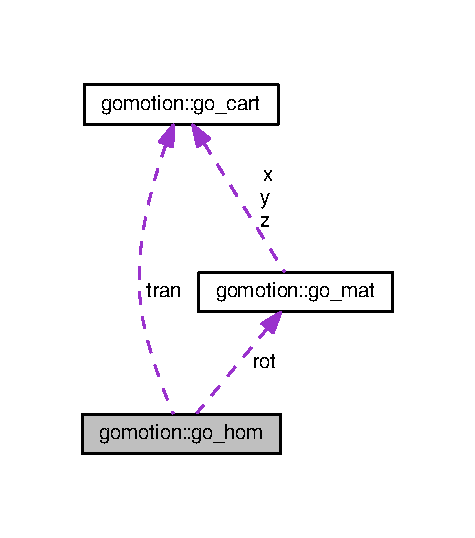
\includegraphics[width=228pt]{d9/dfb/structgomotion_1_1go__hom__coll__graph}
\end{center}
\end{figure}
\subsection*{Data Fields}
\begin{DoxyCompactItemize}
\item 
\hyperlink{structgomotion_1_1go__cart}{go\-\_\-cart} \hyperlink{structgomotion_1_1go__hom_a48557aa558271478688dd08ead8a643e}{tran}
\item 
\hyperlink{structgomotion_1_1go__mat}{go\-\_\-mat} \hyperlink{structgomotion_1_1go__hom_aea63ce241414f57e48ef0fd792d576c6}{rot}
\end{DoxyCompactItemize}


\subsection{Field Documentation}
\hypertarget{structgomotion_1_1go__hom_aea63ce241414f57e48ef0fd792d576c6}{\index{gomotion\-::go\-\_\-hom@{gomotion\-::go\-\_\-hom}!rot@{rot}}
\index{rot@{rot}!gomotion::go_hom@{gomotion\-::go\-\_\-hom}}
\subsubsection[{rot}]{\setlength{\rightskip}{0pt plus 5cm}{\bf go\-\_\-mat} gomotion\-::go\-\_\-hom\-::rot}}\label{structgomotion_1_1go__hom_aea63ce241414f57e48ef0fd792d576c6}
\hypertarget{structgomotion_1_1go__hom_a48557aa558271478688dd08ead8a643e}{\index{gomotion\-::go\-\_\-hom@{gomotion\-::go\-\_\-hom}!tran@{tran}}
\index{tran@{tran}!gomotion::go_hom@{gomotion\-::go\-\_\-hom}}
\subsubsection[{tran}]{\setlength{\rightskip}{0pt plus 5cm}{\bf go\-\_\-cart} gomotion\-::go\-\_\-hom\-::tran}}\label{structgomotion_1_1go__hom_a48557aa558271478688dd08ead8a643e}


The documentation for this struct was generated from the following file\-:\begin{DoxyCompactItemize}
\item 
/usr/local/michalos/nistfanuc\-\_\-ws/src/gomotion/include/gomotion/\hyperlink{gomath_8h}{gomath.\-h}\end{DoxyCompactItemize}

\hypertarget{classgomotion_1_1go__interp}{\section{gomotion\-:\-:go\-\_\-interp Class Reference}
\label{classgomotion_1_1go__interp}\index{gomotion\-::go\-\_\-interp@{gomotion\-::go\-\_\-interp}}
}


The interpolator structure.  




{\ttfamily \#include $<$gointerp.\-h$>$}



Collaboration diagram for gomotion\-:\-:go\-\_\-interp\-:\nopagebreak
\begin{figure}[H]
\begin{center}
\leavevmode
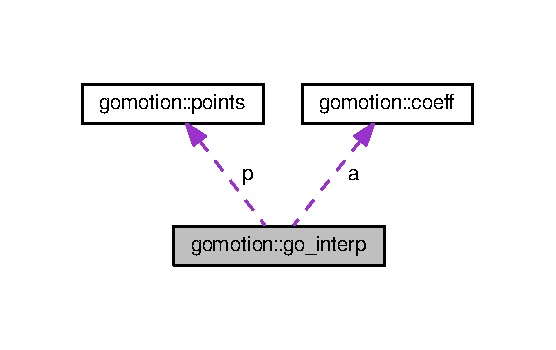
\includegraphics[width=267pt]{d8/dcd/classgomotion_1_1go__interp__coll__graph}
\end{center}
\end{figure}
\subsection*{Public Types}
\begin{DoxyCompactItemize}
\item 
typedef \hyperlink{gotypes_8h_a55d48b38cd959f63c7e8db8337a9792a}{go\-\_\-result}($\ast$ \hyperlink{classgomotion_1_1go__interp_a2e1c3adf730ce4f1e90ea89b33065d1f}{add\-\_\-func} )(\hyperlink{gotypes_8h_afd666a2393eebd71ee455846ac9def9b}{go\-\_\-real} pos)
\item 
typedef \hyperlink{gotypes_8h_afd666a2393eebd71ee455846ac9def9b}{go\-\_\-real}($\ast$ \hyperlink{classgomotion_1_1go__interp_aace47fd625555ec94aed92da3cc3f9ab}{eval\-\_\-func} )(const \hyperlink{gotypes_8h_afd666a2393eebd71ee455846ac9def9b}{go\-\_\-real} t)
\end{DoxyCompactItemize}
\subsection*{Public Member Functions}
\begin{DoxyCompactItemize}
\item 
\hyperlink{gotypes_8h_a55d48b38cd959f63c7e8db8337a9792a}{go\-\_\-result} \hyperlink{classgomotion_1_1go__interp_a12a92abdf88c0edd127a79a82f0fc9c9}{init} ()
\item 
\hyperlink{gotypes_8h_a55d48b38cd959f63c7e8db8337a9792a}{go\-\_\-result} \hyperlink{classgomotion_1_1go__interp_a7119d5c134fb65d3c2d1c5bf6ca48658}{set\-\_\-here} (\hyperlink{gotypes_8h_afd666a2393eebd71ee455846ac9def9b}{go\-\_\-real} here)
\item 
\hyperlink{gotypes_8h_a55d48b38cd959f63c7e8db8337a9792a}{go\-\_\-result} \hyperlink{classgomotion_1_1go__interp_a087a5c025fd9be92962e8231fcdf5806}{calc\-\_\-coeff\-\_\-constant} (const \hyperlink{structgomotion_1_1points}{points} $\ast$\hyperlink{classgomotion_1_1go__interp_ac568f2bc77d7c587637c8340669a5937}{p}, \hyperlink{structgomotion_1_1coeff}{coeff} $\ast$\hyperlink{classgomotion_1_1go__interp_a9ae6dc82a4330b5cb02481ac87169e57}{a})
\item 
\hyperlink{gotypes_8h_a55d48b38cd959f63c7e8db8337a9792a}{go\-\_\-result} \hyperlink{classgomotion_1_1go__interp_a7899a3d65c98c88ac717ba17a7d45a40}{calc\-\_\-coeff\-\_\-linear} (const \hyperlink{structgomotion_1_1points}{points} $\ast$\hyperlink{classgomotion_1_1go__interp_ac568f2bc77d7c587637c8340669a5937}{p}, \hyperlink{structgomotion_1_1coeff}{coeff} $\ast$\hyperlink{classgomotion_1_1go__interp_a9ae6dc82a4330b5cb02481ac87169e57}{a})
\item 
\hyperlink{gotypes_8h_a55d48b38cd959f63c7e8db8337a9792a}{go\-\_\-result} \hyperlink{classgomotion_1_1go__interp_a76b7f017f732629bf8b023266aa51169}{calc\-\_\-coeff\-\_\-cubic\-\_\-bc} (const \hyperlink{structgomotion_1_1points}{points} $\ast$\hyperlink{classgomotion_1_1go__interp_ac568f2bc77d7c587637c8340669a5937}{p}, \hyperlink{structgomotion_1_1coeff}{coeff} $\ast$\hyperlink{classgomotion_1_1go__interp_a9ae6dc82a4330b5cb02481ac87169e57}{a})
\item 
\hyperlink{gotypes_8h_a55d48b38cd959f63c7e8db8337a9792a}{go\-\_\-result} \hyperlink{classgomotion_1_1go__interp_a344b9b93f384d945008a2c442a9e5d12}{calc\-\_\-coeff\-\_\-cubic\-\_\-pf} (const \hyperlink{structgomotion_1_1points}{points} $\ast$\hyperlink{classgomotion_1_1go__interp_ac568f2bc77d7c587637c8340669a5937}{p}, \hyperlink{structgomotion_1_1coeff}{coeff} $\ast$\hyperlink{classgomotion_1_1go__interp_a9ae6dc82a4330b5cb02481ac87169e57}{a})
\item 
\hyperlink{gotypes_8h_a55d48b38cd959f63c7e8db8337a9792a}{go\-\_\-result} \hyperlink{classgomotion_1_1go__interp_a295340be5583d696534a2509763173e2}{calc\-\_\-coeff\-\_\-quintic\-\_\-bc} (const \hyperlink{structgomotion_1_1points}{points} $\ast$\hyperlink{classgomotion_1_1go__interp_ac568f2bc77d7c587637c8340669a5937}{p}, \hyperlink{structgomotion_1_1coeff}{coeff} $\ast$\hyperlink{classgomotion_1_1go__interp_a9ae6dc82a4330b5cb02481ac87169e57}{a})
\item 
\hyperlink{gotypes_8h_a55d48b38cd959f63c7e8db8337a9792a}{go\-\_\-result} \hyperlink{classgomotion_1_1go__interp_a1e5815409f86cd294c1f94e17d993273}{calc\-\_\-coeff\-\_\-quintic\-\_\-pf} (const \hyperlink{structgomotion_1_1points}{points} $\ast$\hyperlink{classgomotion_1_1go__interp_ac568f2bc77d7c587637c8340669a5937}{p}, \hyperlink{structgomotion_1_1coeff}{coeff} $\ast$\hyperlink{classgomotion_1_1go__interp_a9ae6dc82a4330b5cb02481ac87169e57}{a})
\item 
\hyperlink{gotypes_8h_a55d48b38cd959f63c7e8db8337a9792a}{go\-\_\-result} \hyperlink{classgomotion_1_1go__interp_a3a34e58f5f89ed5d1e10cccd27bb01a4}{calc\-\_\-coeff\-\_\-bc} (\hyperlink{gotypes_8h_a7d30f606bb0f58ffe2b3bd71e5c8af5c}{go\-\_\-integer} order, const \hyperlink{structgomotion_1_1points}{points} $\ast$\hyperlink{classgomotion_1_1go__interp_ac568f2bc77d7c587637c8340669a5937}{p}, \hyperlink{structgomotion_1_1coeff}{coeff} $\ast$\hyperlink{classgomotion_1_1go__interp_a9ae6dc82a4330b5cb02481ac87169e57}{a})
\item 
\hyperlink{gotypes_8h_a55d48b38cd959f63c7e8db8337a9792a}{go\-\_\-result} \hyperlink{classgomotion_1_1go__interp_a7eaf3b4e6d89c9435d5709d30f825655}{calc\-\_\-coeff\-\_\-pf} (\hyperlink{gotypes_8h_a7d30f606bb0f58ffe2b3bd71e5c8af5c}{go\-\_\-integer} order, const \hyperlink{structgomotion_1_1points}{points} $\ast$\hyperlink{classgomotion_1_1go__interp_ac568f2bc77d7c587637c8340669a5937}{p}, \hyperlink{structgomotion_1_1coeff}{coeff} $\ast$\hyperlink{classgomotion_1_1go__interp_a9ae6dc82a4330b5cb02481ac87169e57}{a})
\item 
\hyperlink{gotypes_8h_afd666a2393eebd71ee455846ac9def9b}{go\-\_\-real} \hyperlink{classgomotion_1_1go__interp_ab2106b8d532dd3e2b37a8bd5b73f699d}{eval\-\_\-constant} (\hyperlink{gotypes_8h_afd666a2393eebd71ee455846ac9def9b}{go\-\_\-real} t)
\item 
\hyperlink{gotypes_8h_afd666a2393eebd71ee455846ac9def9b}{go\-\_\-real} \hyperlink{classgomotion_1_1go__interp_a856ab9e039af95cc6b07298a3e5dc321}{eval\-\_\-linear} (\hyperlink{gotypes_8h_afd666a2393eebd71ee455846ac9def9b}{go\-\_\-real} t)
\item 
\hyperlink{gotypes_8h_afd666a2393eebd71ee455846ac9def9b}{go\-\_\-real} \hyperlink{classgomotion_1_1go__interp_aa09d64f59f90da484006f8f90e4b88ec}{eval\-\_\-cubic} (\hyperlink{gotypes_8h_afd666a2393eebd71ee455846ac9def9b}{go\-\_\-real} t)
\item 
\hyperlink{gotypes_8h_afd666a2393eebd71ee455846ac9def9b}{go\-\_\-real} \hyperlink{classgomotion_1_1go__interp_ac7da42248cfef9fc204af4a56478c112}{eval\-\_\-quintic} (\hyperlink{gotypes_8h_afd666a2393eebd71ee455846ac9def9b}{go\-\_\-real} t)
\item 
\hyperlink{gotypes_8h_a55d48b38cd959f63c7e8db8337a9792a}{go\-\_\-result} \hyperlink{classgomotion_1_1go__interp_ad8d36b40bae0ffbcd9dd65e1c980bcac}{add\-\_\-constant} (\hyperlink{gotypes_8h_afd666a2393eebd71ee455846ac9def9b}{go\-\_\-real} pos)
\item 
\hyperlink{gotypes_8h_a55d48b38cd959f63c7e8db8337a9792a}{go\-\_\-result} \hyperlink{classgomotion_1_1go__interp_a1347f0aa419953ed253342575d84467d}{add\-\_\-linear} (\hyperlink{gotypes_8h_afd666a2393eebd71ee455846ac9def9b}{go\-\_\-real} pos)
\item 
\hyperlink{gotypes_8h_a55d48b38cd959f63c7e8db8337a9792a}{go\-\_\-result} \hyperlink{classgomotion_1_1go__interp_ac90831ea1decf5c6246804f63442da39}{add\-\_\-cubic\-\_\-pv} (\hyperlink{gotypes_8h_afd666a2393eebd71ee455846ac9def9b}{go\-\_\-real} pos, \hyperlink{gotypes_8h_afd666a2393eebd71ee455846ac9def9b}{go\-\_\-real} vel)
\item 
\hyperlink{gotypes_8h_a55d48b38cd959f63c7e8db8337a9792a}{go\-\_\-result} \hyperlink{classgomotion_1_1go__interp_a773b7a056931239a44b10117ab3c8f0a}{add\-\_\-cubic\-\_\-pdv} (\hyperlink{gotypes_8h_afd666a2393eebd71ee455846ac9def9b}{go\-\_\-real} pos)
\item 
\hyperlink{gotypes_8h_a55d48b38cd959f63c7e8db8337a9792a}{go\-\_\-result} \hyperlink{classgomotion_1_1go__interp_a57fd91ae3b1e836908a167c794c8acc2}{add\-\_\-cubic\-\_\-pf} (\hyperlink{gotypes_8h_afd666a2393eebd71ee455846ac9def9b}{go\-\_\-real} pos)
\item 
\hyperlink{gotypes_8h_a55d48b38cd959f63c7e8db8337a9792a}{go\-\_\-result} \hyperlink{classgomotion_1_1go__interp_a1fdb61083aca63190d3538a14744d9ba}{add\-\_\-quintic\-\_\-pva} (\hyperlink{gotypes_8h_afd666a2393eebd71ee455846ac9def9b}{go\-\_\-real} pos, \hyperlink{gotypes_8h_afd666a2393eebd71ee455846ac9def9b}{go\-\_\-real} vel, \hyperlink{gotypes_8h_afd666a2393eebd71ee455846ac9def9b}{go\-\_\-real} acc)
\item 
\hyperlink{gotypes_8h_a55d48b38cd959f63c7e8db8337a9792a}{go\-\_\-result} \hyperlink{classgomotion_1_1go__interp_a59e7e5d11c608888416fe2cf42fda2ca}{add\-\_\-quintic\-\_\-pvda} (\hyperlink{gotypes_8h_afd666a2393eebd71ee455846ac9def9b}{go\-\_\-real} pos, \hyperlink{gotypes_8h_afd666a2393eebd71ee455846ac9def9b}{go\-\_\-real} vel)
\item 
\hyperlink{gotypes_8h_a55d48b38cd959f63c7e8db8337a9792a}{go\-\_\-result} \hyperlink{classgomotion_1_1go__interp_abce6c8b5f08a01a6f465de1b9d2c1f02}{add\-\_\-quintic\-\_\-pdva} (\hyperlink{gotypes_8h_afd666a2393eebd71ee455846ac9def9b}{go\-\_\-real} pos)
\item 
\hyperlink{gotypes_8h_a55d48b38cd959f63c7e8db8337a9792a}{go\-\_\-result} \hyperlink{classgomotion_1_1go__interp_a1cf92b9ce941bc5db54e7bebc369b6b2}{add\-\_\-quintic\-\_\-pf} (\hyperlink{gotypes_8h_afd666a2393eebd71ee455846ac9def9b}{go\-\_\-real} pos)
\end{DoxyCompactItemize}
\subsection*{Data Fields}
\begin{DoxyCompactItemize}
\item 
\hyperlink{structgomotion_1_1coeff}{coeff} \hyperlink{classgomotion_1_1go__interp_a9ae6dc82a4330b5cb02481ac87169e57}{a}
\item 
\hyperlink{structgomotion_1_1points}{points} \hyperlink{classgomotion_1_1go__interp_ac568f2bc77d7c587637c8340669a5937}{p}
\end{DoxyCompactItemize}


\subsection{Detailed Description}
The interpolator structure. 

For constant-\/ and linear interpolation, exact-\/fit and boundary interpolation is the same, so we only have one type for these. Here we pass single points in succession, and interpolation is done at/between them.

For higher-\/order interpolation, we have two types, exact-\/fit and boundary. For exact-\/fit, we pass single points in succession, and interpolation is done in the middle interval. For boundary, we pass n-\/tuples of pos, vel, accel, etc. and interpolation is done between each tuple.

A variation on boundary interpolation is possible if the derivative values are not known but are estimated by differencing. The functions below suffixed \-\_\-est are used for this. 

\subsection{Member Typedef Documentation}
\hypertarget{classgomotion_1_1go__interp_a2e1c3adf730ce4f1e90ea89b33065d1f}{\index{gomotion\-::go\-\_\-interp@{gomotion\-::go\-\_\-interp}!add\-\_\-func@{add\-\_\-func}}
\index{add\-\_\-func@{add\-\_\-func}!gomotion::go_interp@{gomotion\-::go\-\_\-interp}}
\subsubsection[{add\-\_\-func}]{\setlength{\rightskip}{0pt plus 5cm}typedef {\bf go\-\_\-result}($\ast$ gomotion\-::go\-\_\-interp\-::add\-\_\-func)({\bf go\-\_\-real} pos)}}\label{classgomotion_1_1go__interp_a2e1c3adf730ce4f1e90ea89b33065d1f}
\hypertarget{classgomotion_1_1go__interp_aace47fd625555ec94aed92da3cc3f9ab}{\index{gomotion\-::go\-\_\-interp@{gomotion\-::go\-\_\-interp}!eval\-\_\-func@{eval\-\_\-func}}
\index{eval\-\_\-func@{eval\-\_\-func}!gomotion::go_interp@{gomotion\-::go\-\_\-interp}}
\subsubsection[{eval\-\_\-func}]{\setlength{\rightskip}{0pt plus 5cm}typedef {\bf go\-\_\-real}($\ast$ gomotion\-::go\-\_\-interp\-::eval\-\_\-func)(const {\bf go\-\_\-real} t)}}\label{classgomotion_1_1go__interp_aace47fd625555ec94aed92da3cc3f9ab}


\subsection{Member Function Documentation}
\hypertarget{classgomotion_1_1go__interp_ad8d36b40bae0ffbcd9dd65e1c980bcac}{\index{gomotion\-::go\-\_\-interp@{gomotion\-::go\-\_\-interp}!add\-\_\-constant@{add\-\_\-constant}}
\index{add\-\_\-constant@{add\-\_\-constant}!gomotion::go_interp@{gomotion\-::go\-\_\-interp}}
\subsubsection[{add\-\_\-constant}]{\setlength{\rightskip}{0pt plus 5cm}{\bf go\-\_\-result} gomotion\-::go\-\_\-interp\-::add\-\_\-constant (
\begin{DoxyParamCaption}
\item[{{\bf go\-\_\-real}}]{pos}
\end{DoxyParamCaption}
)}}\label{classgomotion_1_1go__interp_ad8d36b40bae0ffbcd9dd65e1c980bcac}
\hypertarget{classgomotion_1_1go__interp_a773b7a056931239a44b10117ab3c8f0a}{\index{gomotion\-::go\-\_\-interp@{gomotion\-::go\-\_\-interp}!add\-\_\-cubic\-\_\-pdv@{add\-\_\-cubic\-\_\-pdv}}
\index{add\-\_\-cubic\-\_\-pdv@{add\-\_\-cubic\-\_\-pdv}!gomotion::go_interp@{gomotion\-::go\-\_\-interp}}
\subsubsection[{add\-\_\-cubic\-\_\-pdv}]{\setlength{\rightskip}{0pt plus 5cm}{\bf go\-\_\-result} gomotion\-::go\-\_\-interp\-::add\-\_\-cubic\-\_\-pdv (
\begin{DoxyParamCaption}
\item[{{\bf go\-\_\-real}}]{pos}
\end{DoxyParamCaption}
)}}\label{classgomotion_1_1go__interp_a773b7a056931239a44b10117ab3c8f0a}
\hypertarget{classgomotion_1_1go__interp_a57fd91ae3b1e836908a167c794c8acc2}{\index{gomotion\-::go\-\_\-interp@{gomotion\-::go\-\_\-interp}!add\-\_\-cubic\-\_\-pf@{add\-\_\-cubic\-\_\-pf}}
\index{add\-\_\-cubic\-\_\-pf@{add\-\_\-cubic\-\_\-pf}!gomotion::go_interp@{gomotion\-::go\-\_\-interp}}
\subsubsection[{add\-\_\-cubic\-\_\-pf}]{\setlength{\rightskip}{0pt plus 5cm}{\bf go\-\_\-result} gomotion\-::go\-\_\-interp\-::add\-\_\-cubic\-\_\-pf (
\begin{DoxyParamCaption}
\item[{{\bf go\-\_\-real}}]{pos}
\end{DoxyParamCaption}
)}}\label{classgomotion_1_1go__interp_a57fd91ae3b1e836908a167c794c8acc2}
\hypertarget{classgomotion_1_1go__interp_ac90831ea1decf5c6246804f63442da39}{\index{gomotion\-::go\-\_\-interp@{gomotion\-::go\-\_\-interp}!add\-\_\-cubic\-\_\-pv@{add\-\_\-cubic\-\_\-pv}}
\index{add\-\_\-cubic\-\_\-pv@{add\-\_\-cubic\-\_\-pv}!gomotion::go_interp@{gomotion\-::go\-\_\-interp}}
\subsubsection[{add\-\_\-cubic\-\_\-pv}]{\setlength{\rightskip}{0pt plus 5cm}{\bf go\-\_\-result} gomotion\-::go\-\_\-interp\-::add\-\_\-cubic\-\_\-pv (
\begin{DoxyParamCaption}
\item[{{\bf go\-\_\-real}}]{pos, }
\item[{{\bf go\-\_\-real}}]{vel}
\end{DoxyParamCaption}
)}}\label{classgomotion_1_1go__interp_ac90831ea1decf5c6246804f63442da39}
\hypertarget{classgomotion_1_1go__interp_a1347f0aa419953ed253342575d84467d}{\index{gomotion\-::go\-\_\-interp@{gomotion\-::go\-\_\-interp}!add\-\_\-linear@{add\-\_\-linear}}
\index{add\-\_\-linear@{add\-\_\-linear}!gomotion::go_interp@{gomotion\-::go\-\_\-interp}}
\subsubsection[{add\-\_\-linear}]{\setlength{\rightskip}{0pt plus 5cm}{\bf go\-\_\-result} gomotion\-::go\-\_\-interp\-::add\-\_\-linear (
\begin{DoxyParamCaption}
\item[{{\bf go\-\_\-real}}]{pos}
\end{DoxyParamCaption}
)}}\label{classgomotion_1_1go__interp_a1347f0aa419953ed253342575d84467d}
\hypertarget{classgomotion_1_1go__interp_abce6c8b5f08a01a6f465de1b9d2c1f02}{\index{gomotion\-::go\-\_\-interp@{gomotion\-::go\-\_\-interp}!add\-\_\-quintic\-\_\-pdva@{add\-\_\-quintic\-\_\-pdva}}
\index{add\-\_\-quintic\-\_\-pdva@{add\-\_\-quintic\-\_\-pdva}!gomotion::go_interp@{gomotion\-::go\-\_\-interp}}
\subsubsection[{add\-\_\-quintic\-\_\-pdva}]{\setlength{\rightskip}{0pt plus 5cm}{\bf go\-\_\-result} gomotion\-::go\-\_\-interp\-::add\-\_\-quintic\-\_\-pdva (
\begin{DoxyParamCaption}
\item[{{\bf go\-\_\-real}}]{pos}
\end{DoxyParamCaption}
)}}\label{classgomotion_1_1go__interp_abce6c8b5f08a01a6f465de1b9d2c1f02}
\hypertarget{classgomotion_1_1go__interp_a1cf92b9ce941bc5db54e7bebc369b6b2}{\index{gomotion\-::go\-\_\-interp@{gomotion\-::go\-\_\-interp}!add\-\_\-quintic\-\_\-pf@{add\-\_\-quintic\-\_\-pf}}
\index{add\-\_\-quintic\-\_\-pf@{add\-\_\-quintic\-\_\-pf}!gomotion::go_interp@{gomotion\-::go\-\_\-interp}}
\subsubsection[{add\-\_\-quintic\-\_\-pf}]{\setlength{\rightskip}{0pt plus 5cm}{\bf go\-\_\-result} gomotion\-::go\-\_\-interp\-::add\-\_\-quintic\-\_\-pf (
\begin{DoxyParamCaption}
\item[{{\bf go\-\_\-real}}]{pos}
\end{DoxyParamCaption}
)}}\label{classgomotion_1_1go__interp_a1cf92b9ce941bc5db54e7bebc369b6b2}
\hypertarget{classgomotion_1_1go__interp_a1fdb61083aca63190d3538a14744d9ba}{\index{gomotion\-::go\-\_\-interp@{gomotion\-::go\-\_\-interp}!add\-\_\-quintic\-\_\-pva@{add\-\_\-quintic\-\_\-pva}}
\index{add\-\_\-quintic\-\_\-pva@{add\-\_\-quintic\-\_\-pva}!gomotion::go_interp@{gomotion\-::go\-\_\-interp}}
\subsubsection[{add\-\_\-quintic\-\_\-pva}]{\setlength{\rightskip}{0pt plus 5cm}{\bf go\-\_\-result} gomotion\-::go\-\_\-interp\-::add\-\_\-quintic\-\_\-pva (
\begin{DoxyParamCaption}
\item[{{\bf go\-\_\-real}}]{pos, }
\item[{{\bf go\-\_\-real}}]{vel, }
\item[{{\bf go\-\_\-real}}]{acc}
\end{DoxyParamCaption}
)}}\label{classgomotion_1_1go__interp_a1fdb61083aca63190d3538a14744d9ba}
\hypertarget{classgomotion_1_1go__interp_a59e7e5d11c608888416fe2cf42fda2ca}{\index{gomotion\-::go\-\_\-interp@{gomotion\-::go\-\_\-interp}!add\-\_\-quintic\-\_\-pvda@{add\-\_\-quintic\-\_\-pvda}}
\index{add\-\_\-quintic\-\_\-pvda@{add\-\_\-quintic\-\_\-pvda}!gomotion::go_interp@{gomotion\-::go\-\_\-interp}}
\subsubsection[{add\-\_\-quintic\-\_\-pvda}]{\setlength{\rightskip}{0pt plus 5cm}{\bf go\-\_\-result} gomotion\-::go\-\_\-interp\-::add\-\_\-quintic\-\_\-pvda (
\begin{DoxyParamCaption}
\item[{{\bf go\-\_\-real}}]{pos, }
\item[{{\bf go\-\_\-real}}]{vel}
\end{DoxyParamCaption}
)}}\label{classgomotion_1_1go__interp_a59e7e5d11c608888416fe2cf42fda2ca}
\hypertarget{classgomotion_1_1go__interp_a3a34e58f5f89ed5d1e10cccd27bb01a4}{\index{gomotion\-::go\-\_\-interp@{gomotion\-::go\-\_\-interp}!calc\-\_\-coeff\-\_\-bc@{calc\-\_\-coeff\-\_\-bc}}
\index{calc\-\_\-coeff\-\_\-bc@{calc\-\_\-coeff\-\_\-bc}!gomotion::go_interp@{gomotion\-::go\-\_\-interp}}
\subsubsection[{calc\-\_\-coeff\-\_\-bc}]{\setlength{\rightskip}{0pt plus 5cm}{\bf go\-\_\-result} gomotion\-::go\-\_\-interp\-::calc\-\_\-coeff\-\_\-bc (
\begin{DoxyParamCaption}
\item[{{\bf go\-\_\-integer}}]{order, }
\item[{const {\bf points} $\ast$}]{p, }
\item[{{\bf coeff} $\ast$}]{a}
\end{DoxyParamCaption}
)}}\label{classgomotion_1_1go__interp_a3a34e58f5f89ed5d1e10cccd27bb01a4}
\hypertarget{classgomotion_1_1go__interp_a087a5c025fd9be92962e8231fcdf5806}{\index{gomotion\-::go\-\_\-interp@{gomotion\-::go\-\_\-interp}!calc\-\_\-coeff\-\_\-constant@{calc\-\_\-coeff\-\_\-constant}}
\index{calc\-\_\-coeff\-\_\-constant@{calc\-\_\-coeff\-\_\-constant}!gomotion::go_interp@{gomotion\-::go\-\_\-interp}}
\subsubsection[{calc\-\_\-coeff\-\_\-constant}]{\setlength{\rightskip}{0pt plus 5cm}{\bf go\-\_\-result} gomotion\-::go\-\_\-interp\-::calc\-\_\-coeff\-\_\-constant (
\begin{DoxyParamCaption}
\item[{const {\bf points} $\ast$}]{p, }
\item[{{\bf coeff} $\ast$}]{a}
\end{DoxyParamCaption}
)}}\label{classgomotion_1_1go__interp_a087a5c025fd9be92962e8231fcdf5806}
\hypertarget{classgomotion_1_1go__interp_a76b7f017f732629bf8b023266aa51169}{\index{gomotion\-::go\-\_\-interp@{gomotion\-::go\-\_\-interp}!calc\-\_\-coeff\-\_\-cubic\-\_\-bc@{calc\-\_\-coeff\-\_\-cubic\-\_\-bc}}
\index{calc\-\_\-coeff\-\_\-cubic\-\_\-bc@{calc\-\_\-coeff\-\_\-cubic\-\_\-bc}!gomotion::go_interp@{gomotion\-::go\-\_\-interp}}
\subsubsection[{calc\-\_\-coeff\-\_\-cubic\-\_\-bc}]{\setlength{\rightskip}{0pt plus 5cm}{\bf go\-\_\-result} gomotion\-::go\-\_\-interp\-::calc\-\_\-coeff\-\_\-cubic\-\_\-bc (
\begin{DoxyParamCaption}
\item[{const {\bf points} $\ast$}]{p, }
\item[{{\bf coeff} $\ast$}]{a}
\end{DoxyParamCaption}
)}}\label{classgomotion_1_1go__interp_a76b7f017f732629bf8b023266aa51169}
\hypertarget{classgomotion_1_1go__interp_a344b9b93f384d945008a2c442a9e5d12}{\index{gomotion\-::go\-\_\-interp@{gomotion\-::go\-\_\-interp}!calc\-\_\-coeff\-\_\-cubic\-\_\-pf@{calc\-\_\-coeff\-\_\-cubic\-\_\-pf}}
\index{calc\-\_\-coeff\-\_\-cubic\-\_\-pf@{calc\-\_\-coeff\-\_\-cubic\-\_\-pf}!gomotion::go_interp@{gomotion\-::go\-\_\-interp}}
\subsubsection[{calc\-\_\-coeff\-\_\-cubic\-\_\-pf}]{\setlength{\rightskip}{0pt plus 5cm}{\bf go\-\_\-result} gomotion\-::go\-\_\-interp\-::calc\-\_\-coeff\-\_\-cubic\-\_\-pf (
\begin{DoxyParamCaption}
\item[{const {\bf points} $\ast$}]{p, }
\item[{{\bf coeff} $\ast$}]{a}
\end{DoxyParamCaption}
)}}\label{classgomotion_1_1go__interp_a344b9b93f384d945008a2c442a9e5d12}
\hypertarget{classgomotion_1_1go__interp_a7899a3d65c98c88ac717ba17a7d45a40}{\index{gomotion\-::go\-\_\-interp@{gomotion\-::go\-\_\-interp}!calc\-\_\-coeff\-\_\-linear@{calc\-\_\-coeff\-\_\-linear}}
\index{calc\-\_\-coeff\-\_\-linear@{calc\-\_\-coeff\-\_\-linear}!gomotion::go_interp@{gomotion\-::go\-\_\-interp}}
\subsubsection[{calc\-\_\-coeff\-\_\-linear}]{\setlength{\rightskip}{0pt plus 5cm}{\bf go\-\_\-result} gomotion\-::go\-\_\-interp\-::calc\-\_\-coeff\-\_\-linear (
\begin{DoxyParamCaption}
\item[{const {\bf points} $\ast$}]{p, }
\item[{{\bf coeff} $\ast$}]{a}
\end{DoxyParamCaption}
)}}\label{classgomotion_1_1go__interp_a7899a3d65c98c88ac717ba17a7d45a40}
\hypertarget{classgomotion_1_1go__interp_a7eaf3b4e6d89c9435d5709d30f825655}{\index{gomotion\-::go\-\_\-interp@{gomotion\-::go\-\_\-interp}!calc\-\_\-coeff\-\_\-pf@{calc\-\_\-coeff\-\_\-pf}}
\index{calc\-\_\-coeff\-\_\-pf@{calc\-\_\-coeff\-\_\-pf}!gomotion::go_interp@{gomotion\-::go\-\_\-interp}}
\subsubsection[{calc\-\_\-coeff\-\_\-pf}]{\setlength{\rightskip}{0pt plus 5cm}{\bf go\-\_\-result} gomotion\-::go\-\_\-interp\-::calc\-\_\-coeff\-\_\-pf (
\begin{DoxyParamCaption}
\item[{{\bf go\-\_\-integer}}]{order, }
\item[{const {\bf points} $\ast$}]{p, }
\item[{{\bf coeff} $\ast$}]{a}
\end{DoxyParamCaption}
)}}\label{classgomotion_1_1go__interp_a7eaf3b4e6d89c9435d5709d30f825655}
\hypertarget{classgomotion_1_1go__interp_a295340be5583d696534a2509763173e2}{\index{gomotion\-::go\-\_\-interp@{gomotion\-::go\-\_\-interp}!calc\-\_\-coeff\-\_\-quintic\-\_\-bc@{calc\-\_\-coeff\-\_\-quintic\-\_\-bc}}
\index{calc\-\_\-coeff\-\_\-quintic\-\_\-bc@{calc\-\_\-coeff\-\_\-quintic\-\_\-bc}!gomotion::go_interp@{gomotion\-::go\-\_\-interp}}
\subsubsection[{calc\-\_\-coeff\-\_\-quintic\-\_\-bc}]{\setlength{\rightskip}{0pt plus 5cm}{\bf go\-\_\-result} gomotion\-::go\-\_\-interp\-::calc\-\_\-coeff\-\_\-quintic\-\_\-bc (
\begin{DoxyParamCaption}
\item[{const {\bf points} $\ast$}]{p, }
\item[{{\bf coeff} $\ast$}]{a}
\end{DoxyParamCaption}
)}}\label{classgomotion_1_1go__interp_a295340be5583d696534a2509763173e2}
\hypertarget{classgomotion_1_1go__interp_a1e5815409f86cd294c1f94e17d993273}{\index{gomotion\-::go\-\_\-interp@{gomotion\-::go\-\_\-interp}!calc\-\_\-coeff\-\_\-quintic\-\_\-pf@{calc\-\_\-coeff\-\_\-quintic\-\_\-pf}}
\index{calc\-\_\-coeff\-\_\-quintic\-\_\-pf@{calc\-\_\-coeff\-\_\-quintic\-\_\-pf}!gomotion::go_interp@{gomotion\-::go\-\_\-interp}}
\subsubsection[{calc\-\_\-coeff\-\_\-quintic\-\_\-pf}]{\setlength{\rightskip}{0pt plus 5cm}{\bf go\-\_\-result} gomotion\-::go\-\_\-interp\-::calc\-\_\-coeff\-\_\-quintic\-\_\-pf (
\begin{DoxyParamCaption}
\item[{const {\bf points} $\ast$}]{p, }
\item[{{\bf coeff} $\ast$}]{a}
\end{DoxyParamCaption}
)}}\label{classgomotion_1_1go__interp_a1e5815409f86cd294c1f94e17d993273}
\hypertarget{classgomotion_1_1go__interp_ab2106b8d532dd3e2b37a8bd5b73f699d}{\index{gomotion\-::go\-\_\-interp@{gomotion\-::go\-\_\-interp}!eval\-\_\-constant@{eval\-\_\-constant}}
\index{eval\-\_\-constant@{eval\-\_\-constant}!gomotion::go_interp@{gomotion\-::go\-\_\-interp}}
\subsubsection[{eval\-\_\-constant}]{\setlength{\rightskip}{0pt plus 5cm}{\bf go\-\_\-real} gomotion\-::go\-\_\-interp\-::eval\-\_\-constant (
\begin{DoxyParamCaption}
\item[{{\bf go\-\_\-real}}]{t}
\end{DoxyParamCaption}
)}}\label{classgomotion_1_1go__interp_ab2106b8d532dd3e2b37a8bd5b73f699d}
\hypertarget{classgomotion_1_1go__interp_aa09d64f59f90da484006f8f90e4b88ec}{\index{gomotion\-::go\-\_\-interp@{gomotion\-::go\-\_\-interp}!eval\-\_\-cubic@{eval\-\_\-cubic}}
\index{eval\-\_\-cubic@{eval\-\_\-cubic}!gomotion::go_interp@{gomotion\-::go\-\_\-interp}}
\subsubsection[{eval\-\_\-cubic}]{\setlength{\rightskip}{0pt plus 5cm}{\bf go\-\_\-real} gomotion\-::go\-\_\-interp\-::eval\-\_\-cubic (
\begin{DoxyParamCaption}
\item[{{\bf go\-\_\-real}}]{t}
\end{DoxyParamCaption}
)}}\label{classgomotion_1_1go__interp_aa09d64f59f90da484006f8f90e4b88ec}
\hypertarget{classgomotion_1_1go__interp_a856ab9e039af95cc6b07298a3e5dc321}{\index{gomotion\-::go\-\_\-interp@{gomotion\-::go\-\_\-interp}!eval\-\_\-linear@{eval\-\_\-linear}}
\index{eval\-\_\-linear@{eval\-\_\-linear}!gomotion::go_interp@{gomotion\-::go\-\_\-interp}}
\subsubsection[{eval\-\_\-linear}]{\setlength{\rightskip}{0pt plus 5cm}{\bf go\-\_\-real} gomotion\-::go\-\_\-interp\-::eval\-\_\-linear (
\begin{DoxyParamCaption}
\item[{{\bf go\-\_\-real}}]{t}
\end{DoxyParamCaption}
)}}\label{classgomotion_1_1go__interp_a856ab9e039af95cc6b07298a3e5dc321}
\hypertarget{classgomotion_1_1go__interp_ac7da42248cfef9fc204af4a56478c112}{\index{gomotion\-::go\-\_\-interp@{gomotion\-::go\-\_\-interp}!eval\-\_\-quintic@{eval\-\_\-quintic}}
\index{eval\-\_\-quintic@{eval\-\_\-quintic}!gomotion::go_interp@{gomotion\-::go\-\_\-interp}}
\subsubsection[{eval\-\_\-quintic}]{\setlength{\rightskip}{0pt plus 5cm}{\bf go\-\_\-real} gomotion\-::go\-\_\-interp\-::eval\-\_\-quintic (
\begin{DoxyParamCaption}
\item[{{\bf go\-\_\-real}}]{t}
\end{DoxyParamCaption}
)}}\label{classgomotion_1_1go__interp_ac7da42248cfef9fc204af4a56478c112}
\hypertarget{classgomotion_1_1go__interp_a12a92abdf88c0edd127a79a82f0fc9c9}{\index{gomotion\-::go\-\_\-interp@{gomotion\-::go\-\_\-interp}!init@{init}}
\index{init@{init}!gomotion::go_interp@{gomotion\-::go\-\_\-interp}}
\subsubsection[{init}]{\setlength{\rightskip}{0pt plus 5cm}{\bf go\-\_\-result} gomotion\-::go\-\_\-interp\-::init (
\begin{DoxyParamCaption}
{}
\end{DoxyParamCaption}
)}}\label{classgomotion_1_1go__interp_a12a92abdf88c0edd127a79a82f0fc9c9}
\hypertarget{classgomotion_1_1go__interp_a7119d5c134fb65d3c2d1c5bf6ca48658}{\index{gomotion\-::go\-\_\-interp@{gomotion\-::go\-\_\-interp}!set\-\_\-here@{set\-\_\-here}}
\index{set\-\_\-here@{set\-\_\-here}!gomotion::go_interp@{gomotion\-::go\-\_\-interp}}
\subsubsection[{set\-\_\-here}]{\setlength{\rightskip}{0pt plus 5cm}{\bf go\-\_\-result} gomotion\-::go\-\_\-interp\-::set\-\_\-here (
\begin{DoxyParamCaption}
\item[{{\bf go\-\_\-real}}]{here}
\end{DoxyParamCaption}
)}}\label{classgomotion_1_1go__interp_a7119d5c134fb65d3c2d1c5bf6ca48658}


\subsection{Field Documentation}
\hypertarget{classgomotion_1_1go__interp_a9ae6dc82a4330b5cb02481ac87169e57}{\index{gomotion\-::go\-\_\-interp@{gomotion\-::go\-\_\-interp}!a@{a}}
\index{a@{a}!gomotion::go_interp@{gomotion\-::go\-\_\-interp}}
\subsubsection[{a}]{\setlength{\rightskip}{0pt plus 5cm}{\bf coeff} gomotion\-::go\-\_\-interp\-::a}}\label{classgomotion_1_1go__interp_a9ae6dc82a4330b5cb02481ac87169e57}
\hypertarget{classgomotion_1_1go__interp_ac568f2bc77d7c587637c8340669a5937}{\index{gomotion\-::go\-\_\-interp@{gomotion\-::go\-\_\-interp}!p@{p}}
\index{p@{p}!gomotion::go_interp@{gomotion\-::go\-\_\-interp}}
\subsubsection[{p}]{\setlength{\rightskip}{0pt plus 5cm}{\bf points} gomotion\-::go\-\_\-interp\-::p}}\label{classgomotion_1_1go__interp_ac568f2bc77d7c587637c8340669a5937}


The documentation for this class was generated from the following files\-:\begin{DoxyCompactItemize}
\item 
/usr/local/michalos/nistfanuc\-\_\-ws/src/gomotion/include/gomotion/\hyperlink{gointerp_8h}{gointerp.\-h}\item 
/usr/local/michalos/nistfanuc\-\_\-ws/src/gomotion/src/\hyperlink{gointerp_8cpp}{gointerp.\-cpp}\end{DoxyCompactItemize}

\hypertarget{structgomotion_1_1go__line}{\section{gomotion\-:\-:go\-\_\-line Struct Reference}
\label{structgomotion_1_1go__line}\index{gomotion\-::go\-\_\-line@{gomotion\-::go\-\_\-line}}
}


{\ttfamily \#include $<$gomath.\-h$>$}



Collaboration diagram for gomotion\-:\-:go\-\_\-line\-:\nopagebreak
\begin{figure}[H]
\begin{center}
\leavevmode
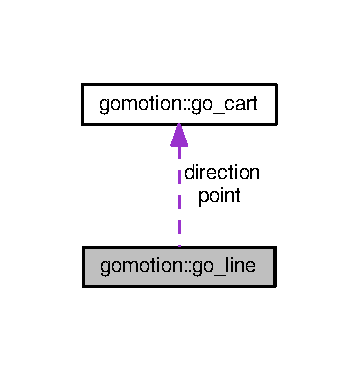
\includegraphics[width=172pt]{d1/df8/structgomotion_1_1go__line__coll__graph}
\end{center}
\end{figure}
\subsection*{Data Fields}
\begin{DoxyCompactItemize}
\item 
\hyperlink{structgomotion_1_1go__cart}{go\-\_\-cart} \hyperlink{structgomotion_1_1go__line_a074cee7c1f473ac10092e38e3f73699e}{point}
\item 
\hyperlink{structgomotion_1_1go__cart}{go\-\_\-cart} \hyperlink{structgomotion_1_1go__line_ae6dce3a84c609e8ef3c3d97b8a5bc0ab}{direction}
\end{DoxyCompactItemize}


\subsection{Detailed Description}
Lines are represented in point-\/direction form (point p, direction v) as (x -\/ px)/vx = (y -\/ py)/vy = (z -\/ pz)vz 

\subsection{Field Documentation}
\hypertarget{structgomotion_1_1go__line_ae6dce3a84c609e8ef3c3d97b8a5bc0ab}{\index{gomotion\-::go\-\_\-line@{gomotion\-::go\-\_\-line}!direction@{direction}}
\index{direction@{direction}!gomotion::go_line@{gomotion\-::go\-\_\-line}}
\subsubsection[{direction}]{\setlength{\rightskip}{0pt plus 5cm}{\bf go\-\_\-cart} gomotion\-::go\-\_\-line\-::direction}}\label{structgomotion_1_1go__line_ae6dce3a84c609e8ef3c3d97b8a5bc0ab}
\hypertarget{structgomotion_1_1go__line_a074cee7c1f473ac10092e38e3f73699e}{\index{gomotion\-::go\-\_\-line@{gomotion\-::go\-\_\-line}!point@{point}}
\index{point@{point}!gomotion::go_line@{gomotion\-::go\-\_\-line}}
\subsubsection[{point}]{\setlength{\rightskip}{0pt plus 5cm}{\bf go\-\_\-cart} gomotion\-::go\-\_\-line\-::point}}\label{structgomotion_1_1go__line_a074cee7c1f473ac10092e38e3f73699e}


The documentation for this struct was generated from the following file\-:\begin{DoxyCompactItemize}
\item 
/usr/local/michalos/nistfanuc\-\_\-ws/src/gomotion/include/gomotion/\hyperlink{gomath_8h}{gomath.\-h}\end{DoxyCompactItemize}

\hypertarget{structgomotion_1_1go__link}{\section{gomotion\-:\-:go\-\_\-link Struct Reference}
\label{structgomotion_1_1go__link}\index{gomotion\-::go\-\_\-link@{gomotion\-::go\-\_\-link}}
}


{\ttfamily \#include $<$gomath.\-h$>$}



Collaboration diagram for gomotion\-:\-:go\-\_\-link\-:\nopagebreak
\begin{figure}[H]
\begin{center}
\leavevmode
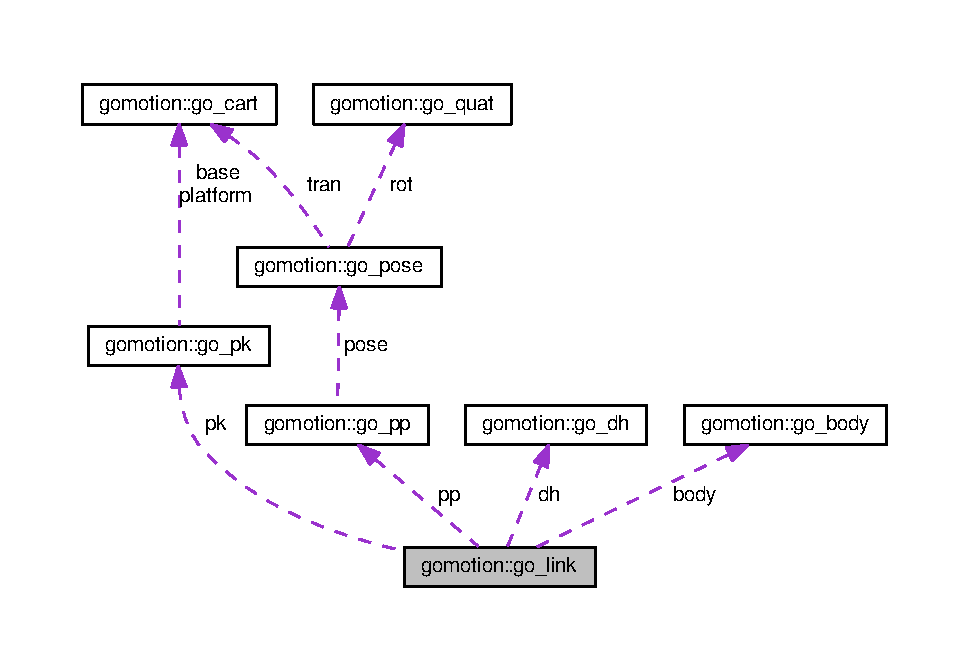
\includegraphics[width=350pt]{d1/de8/structgomotion_1_1go__link__coll__graph}
\end{center}
\end{figure}
\subsection*{Data Fields}
\begin{DoxyCompactItemize}
\item 
\begin{tabbing}
xx\=xx\=xx\=xx\=xx\=xx\=xx\=xx\=xx\=\kill
union \{\\
\>\hyperlink{structgomotion_1_1go__dh}{go\_dh} \hyperlink{structgomotion_1_1go__link_acb0559852ab118cc11f102bb11ff9811}{dh}\\
\>\hyperlink{structgomotion_1_1go__pk}{go\_pk} \hyperlink{structgomotion_1_1go__link_a681e1395c9921b192466d8a27c348d4d}{pk}\\
\>\hyperlink{structgomotion_1_1go__pp}{go\_pp} \hyperlink{structgomotion_1_1go__link_aeb6fd1a42fc5194080ffa0f89dae8e20}{pp}\\
\} \hyperlink{structgomotion_1_1go__link_aacb42b16b578a2fbf1b7c25b18cafe2b}{u}\\

\end{tabbing}\item 
\hyperlink{structgomotion_1_1go__body}{go\-\_\-body} \hyperlink{structgomotion_1_1go__link_a27aa5b81fdb2402883899a11375891c3}{body}
\item 
\hyperlink{gotypes_8h_ae890d9a0ddecc0d3073622cc4312092d}{go\-\_\-flag} \hyperlink{structgomotion_1_1go__link_ad159e1d034c86635efc11a6b0c34dc7e}{type}
\item 
\hyperlink{gotypes_8h_ae890d9a0ddecc0d3073622cc4312092d}{go\-\_\-flag} \hyperlink{structgomotion_1_1go__link_aa70635d6c7483d989c6cd8c0616145a5}{quantity}
\end{DoxyCompactItemize}


\subsection{Detailed Description}
This is the generic link structure for P\-K\-M sliding/cable links and serial revolute/prismatic links. 

\subsection{Field Documentation}
\hypertarget{structgomotion_1_1go__link_a27aa5b81fdb2402883899a11375891c3}{\index{gomotion\-::go\-\_\-link@{gomotion\-::go\-\_\-link}!body@{body}}
\index{body@{body}!gomotion::go_link@{gomotion\-::go\-\_\-link}}
\subsubsection[{body}]{\setlength{\rightskip}{0pt plus 5cm}{\bf go\-\_\-body} gomotion\-::go\-\_\-link\-::body}}\label{structgomotion_1_1go__link_a27aa5b81fdb2402883899a11375891c3}
the link's rigid body parameters \hypertarget{structgomotion_1_1go__link_acb0559852ab118cc11f102bb11ff9811}{\index{gomotion\-::go\-\_\-link@{gomotion\-::go\-\_\-link}!dh@{dh}}
\index{dh@{dh}!gomotion::go_link@{gomotion\-::go\-\_\-link}}
\subsubsection[{dh}]{\setlength{\rightskip}{0pt plus 5cm}{\bf go\-\_\-dh} gomotion\-::go\-\_\-link\-::dh}}\label{structgomotion_1_1go__link_acb0559852ab118cc11f102bb11ff9811}
if you have D\-H params and don't want to convert to P\-P \hypertarget{structgomotion_1_1go__link_a681e1395c9921b192466d8a27c348d4d}{\index{gomotion\-::go\-\_\-link@{gomotion\-::go\-\_\-link}!pk@{pk}}
\index{pk@{pk}!gomotion::go_link@{gomotion\-::go\-\_\-link}}
\subsubsection[{pk}]{\setlength{\rightskip}{0pt plus 5cm}{\bf go\-\_\-pk} gomotion\-::go\-\_\-link\-::pk}}\label{structgomotion_1_1go__link_a681e1395c9921b192466d8a27c348d4d}
if you have a parallel machine, e.\-g., hexapod or robot crane \hypertarget{structgomotion_1_1go__link_aeb6fd1a42fc5194080ffa0f89dae8e20}{\index{gomotion\-::go\-\_\-link@{gomotion\-::go\-\_\-link}!pp@{pp}}
\index{pp@{pp}!gomotion::go_link@{gomotion\-::go\-\_\-link}}
\subsubsection[{pp}]{\setlength{\rightskip}{0pt plus 5cm}{\bf go\-\_\-pp} gomotion\-::go\-\_\-link\-::pp}}\label{structgomotion_1_1go__link_aeb6fd1a42fc5194080ffa0f89dae8e20}
if you have a serial machine, e.\-g., an industrial robot \hypertarget{structgomotion_1_1go__link_aa70635d6c7483d989c6cd8c0616145a5}{\index{gomotion\-::go\-\_\-link@{gomotion\-::go\-\_\-link}!quantity@{quantity}}
\index{quantity@{quantity}!gomotion::go_link@{gomotion\-::go\-\_\-link}}
\subsubsection[{quantity}]{\setlength{\rightskip}{0pt plus 5cm}{\bf go\-\_\-flag} gomotion\-::go\-\_\-link\-::quantity}}\label{structgomotion_1_1go__link_aa70635d6c7483d989c6cd8c0616145a5}
one of G\-O\-\_\-\-Q\-U\-A\-N\-T\-I\-T\-Y\-\_\-\-L\-E\-N\-G\-T\-H,A\-N\-G\-L\-E \hypertarget{structgomotion_1_1go__link_ad159e1d034c86635efc11a6b0c34dc7e}{\index{gomotion\-::go\-\_\-link@{gomotion\-::go\-\_\-link}!type@{type}}
\index{type@{type}!gomotion::go_link@{gomotion\-::go\-\_\-link}}
\subsubsection[{type}]{\setlength{\rightskip}{0pt plus 5cm}{\bf go\-\_\-flag} gomotion\-::go\-\_\-link\-::type}}\label{structgomotion_1_1go__link_ad159e1d034c86635efc11a6b0c34dc7e}
one of G\-O\-\_\-\-L\-I\-N\-K\-\_\-\-D\-H,P\-K,P\-P \hypertarget{structgomotion_1_1go__link_aacb42b16b578a2fbf1b7c25b18cafe2b}{\index{gomotion\-::go\-\_\-link@{gomotion\-::go\-\_\-link}!u@{u}}
\index{u@{u}!gomotion::go_link@{gomotion\-::go\-\_\-link}}
\subsubsection[{u}]{\setlength{\rightskip}{0pt plus 5cm}union \{ ... \}   gomotion\-::go\-\_\-link\-::u}}\label{structgomotion_1_1go__link_aacb42b16b578a2fbf1b7c25b18cafe2b}


The documentation for this struct was generated from the following file\-:\begin{DoxyCompactItemize}
\item 
/usr/local/michalos/nistfanuc\-\_\-ws/src/gomotion/include/gomotion/\hyperlink{gomath_8h}{gomath.\-h}\end{DoxyCompactItemize}

\hypertarget{structgomotion_1_1go__mat}{\section{gomotion\-:\-:go\-\_\-mat Struct Reference}
\label{structgomotion_1_1go__mat}\index{gomotion\-::go\-\_\-mat@{gomotion\-::go\-\_\-mat}}
}


{\ttfamily \#include $<$gomath.\-h$>$}



Collaboration diagram for gomotion\-:\-:go\-\_\-mat\-:\nopagebreak
\begin{figure}[H]
\begin{center}
\leavevmode
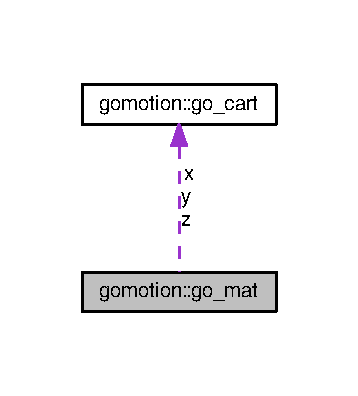
\includegraphics[width=172pt]{dd/d7f/structgomotion_1_1go__mat__coll__graph}
\end{center}
\end{figure}
\subsection*{Data Fields}
\begin{DoxyCompactItemize}
\item 
\hyperlink{structgomotion_1_1go__cart}{go\-\_\-cart} \hyperlink{structgomotion_1_1go__mat_a53b13939d829ceb25ad338899cc41ebb}{x}
\item 
\hyperlink{structgomotion_1_1go__cart}{go\-\_\-cart} \hyperlink{structgomotion_1_1go__mat_a77d00fb0a019de108943dc3510db99d7}{y}
\item 
\hyperlink{structgomotion_1_1go__cart}{go\-\_\-cart} \hyperlink{structgomotion_1_1go__mat_ab6b8b051c8695a4a07da09a4b76da95e}{z}
\end{DoxyCompactItemize}


\subsection{Detailed Description}
A rotation matrix. 

\subsection{Field Documentation}
\hypertarget{structgomotion_1_1go__mat_a53b13939d829ceb25ad338899cc41ebb}{\index{gomotion\-::go\-\_\-mat@{gomotion\-::go\-\_\-mat}!x@{x}}
\index{x@{x}!gomotion::go_mat@{gomotion\-::go\-\_\-mat}}
\subsubsection[{x}]{\setlength{\rightskip}{0pt plus 5cm}{\bf go\-\_\-cart} gomotion\-::go\-\_\-mat\-::x}}\label{structgomotion_1_1go__mat_a53b13939d829ceb25ad338899cc41ebb}
X unit vector \hypertarget{structgomotion_1_1go__mat_a77d00fb0a019de108943dc3510db99d7}{\index{gomotion\-::go\-\_\-mat@{gomotion\-::go\-\_\-mat}!y@{y}}
\index{y@{y}!gomotion::go_mat@{gomotion\-::go\-\_\-mat}}
\subsubsection[{y}]{\setlength{\rightskip}{0pt plus 5cm}{\bf go\-\_\-cart} gomotion\-::go\-\_\-mat\-::y}}\label{structgomotion_1_1go__mat_a77d00fb0a019de108943dc3510db99d7}
Y unit vector \hypertarget{structgomotion_1_1go__mat_ab6b8b051c8695a4a07da09a4b76da95e}{\index{gomotion\-::go\-\_\-mat@{gomotion\-::go\-\_\-mat}!z@{z}}
\index{z@{z}!gomotion::go_mat@{gomotion\-::go\-\_\-mat}}
\subsubsection[{z}]{\setlength{\rightskip}{0pt plus 5cm}{\bf go\-\_\-cart} gomotion\-::go\-\_\-mat\-::z}}\label{structgomotion_1_1go__mat_ab6b8b051c8695a4a07da09a4b76da95e}
Z unit vector 

The documentation for this struct was generated from the following file\-:\begin{DoxyCompactItemize}
\item 
/usr/local/michalos/nistfanuc\-\_\-ws/src/gomotion/include/gomotion/\hyperlink{gomath_8h}{gomath.\-h}\end{DoxyCompactItemize}

\hypertarget{structgomotion_1_1go__matrix}{\section{gomotion\-:\-:go\-\_\-matrix Struct Reference}
\label{structgomotion_1_1go__matrix}\index{gomotion\-::go\-\_\-matrix@{gomotion\-::go\-\_\-matrix}}
}


{\ttfamily \#include $<$gomath.\-h$>$}

\subsection*{Data Fields}
\begin{DoxyCompactItemize}
\item 
\hyperlink{gotypes_8h_a7d30f606bb0f58ffe2b3bd71e5c8af5c}{go\-\_\-integer} \hyperlink{structgomotion_1_1go__matrix_a7e46395453eb9731459d73cbaadd2cdf}{rows}
\item 
\hyperlink{gotypes_8h_a7d30f606bb0f58ffe2b3bd71e5c8af5c}{go\-\_\-integer} \hyperlink{structgomotion_1_1go__matrix_ab0f71737a0cd9fa476e687273f7cbbfb}{cols}
\item 
\hyperlink{gotypes_8h_afd666a2393eebd71ee455846ac9def9b}{go\-\_\-real} $\ast$$\ast$ \hyperlink{structgomotion_1_1go__matrix_ae1f2f89628116a3dc2b4282a01456678}{el}
\item 
\hyperlink{gotypes_8h_afd666a2393eebd71ee455846ac9def9b}{go\-\_\-real} $\ast$$\ast$ \hyperlink{structgomotion_1_1go__matrix_a4e37308ef1e80920a816adf1aa99f66d}{elcpy}
\item 
\hyperlink{gotypes_8h_afd666a2393eebd71ee455846ac9def9b}{go\-\_\-real} $\ast$ \hyperlink{structgomotion_1_1go__matrix_a46242c485b2f46d23f6b4997cb382392}{v}
\item 
\hyperlink{gotypes_8h_a7d30f606bb0f58ffe2b3bd71e5c8af5c}{go\-\_\-integer} $\ast$ \hyperlink{structgomotion_1_1go__matrix_a90ce357ba1351c682da4cf98e8a238bb}{index}
\end{DoxyCompactItemize}


\subsection{Field Documentation}
\hypertarget{structgomotion_1_1go__matrix_ab0f71737a0cd9fa476e687273f7cbbfb}{\index{gomotion\-::go\-\_\-matrix@{gomotion\-::go\-\_\-matrix}!cols@{cols}}
\index{cols@{cols}!gomotion::go_matrix@{gomotion\-::go\-\_\-matrix}}
\subsubsection[{cols}]{\setlength{\rightskip}{0pt plus 5cm}{\bf go\-\_\-integer} gomotion\-::go\-\_\-matrix\-::cols}}\label{structgomotion_1_1go__matrix_ab0f71737a0cd9fa476e687273f7cbbfb}
\hypertarget{structgomotion_1_1go__matrix_ae1f2f89628116a3dc2b4282a01456678}{\index{gomotion\-::go\-\_\-matrix@{gomotion\-::go\-\_\-matrix}!el@{el}}
\index{el@{el}!gomotion::go_matrix@{gomotion\-::go\-\_\-matrix}}
\subsubsection[{el}]{\setlength{\rightskip}{0pt plus 5cm}{\bf go\-\_\-real}$\ast$$\ast$ gomotion\-::go\-\_\-matrix\-::el}}\label{structgomotion_1_1go__matrix_ae1f2f89628116a3dc2b4282a01456678}
\hypertarget{structgomotion_1_1go__matrix_a4e37308ef1e80920a816adf1aa99f66d}{\index{gomotion\-::go\-\_\-matrix@{gomotion\-::go\-\_\-matrix}!elcpy@{elcpy}}
\index{elcpy@{elcpy}!gomotion::go_matrix@{gomotion\-::go\-\_\-matrix}}
\subsubsection[{elcpy}]{\setlength{\rightskip}{0pt plus 5cm}{\bf go\-\_\-real}$\ast$$\ast$ gomotion\-::go\-\_\-matrix\-::elcpy}}\label{structgomotion_1_1go__matrix_a4e37308ef1e80920a816adf1aa99f66d}
\hypertarget{structgomotion_1_1go__matrix_a90ce357ba1351c682da4cf98e8a238bb}{\index{gomotion\-::go\-\_\-matrix@{gomotion\-::go\-\_\-matrix}!index@{index}}
\index{index@{index}!gomotion::go_matrix@{gomotion\-::go\-\_\-matrix}}
\subsubsection[{index}]{\setlength{\rightskip}{0pt plus 5cm}{\bf go\-\_\-integer}$\ast$ gomotion\-::go\-\_\-matrix\-::index}}\label{structgomotion_1_1go__matrix_a90ce357ba1351c682da4cf98e8a238bb}
\hypertarget{structgomotion_1_1go__matrix_a7e46395453eb9731459d73cbaadd2cdf}{\index{gomotion\-::go\-\_\-matrix@{gomotion\-::go\-\_\-matrix}!rows@{rows}}
\index{rows@{rows}!gomotion::go_matrix@{gomotion\-::go\-\_\-matrix}}
\subsubsection[{rows}]{\setlength{\rightskip}{0pt plus 5cm}{\bf go\-\_\-integer} gomotion\-::go\-\_\-matrix\-::rows}}\label{structgomotion_1_1go__matrix_a7e46395453eb9731459d73cbaadd2cdf}
\hypertarget{structgomotion_1_1go__matrix_a46242c485b2f46d23f6b4997cb382392}{\index{gomotion\-::go\-\_\-matrix@{gomotion\-::go\-\_\-matrix}!v@{v}}
\index{v@{v}!gomotion::go_matrix@{gomotion\-::go\-\_\-matrix}}
\subsubsection[{v}]{\setlength{\rightskip}{0pt plus 5cm}{\bf go\-\_\-real}$\ast$ gomotion\-::go\-\_\-matrix\-::v}}\label{structgomotion_1_1go__matrix_a46242c485b2f46d23f6b4997cb382392}


The documentation for this struct was generated from the following file\-:\begin{DoxyCompactItemize}
\item 
/usr/local/michalos/nistfanuc\-\_\-ws/src/gomotion/include/gomotion/\hyperlink{gomath_8h}{gomath.\-h}\end{DoxyCompactItemize}

\hypertarget{structgomotion_1_1go__motion__circular__params}{\section{gomotion\-:\-:go\-\_\-motion\-\_\-circular\-\_\-params Struct Reference}
\label{structgomotion_1_1go__motion__circular__params}\index{gomotion\-::go\-\_\-motion\-\_\-circular\-\_\-params@{gomotion\-::go\-\_\-motion\-\_\-circular\-\_\-params}}
}


{\ttfamily \#include $<$gomotion.\-h$>$}



Collaboration diagram for gomotion\-:\-:go\-\_\-motion\-\_\-circular\-\_\-params\-:\nopagebreak
\begin{figure}[H]
\begin{center}
\leavevmode
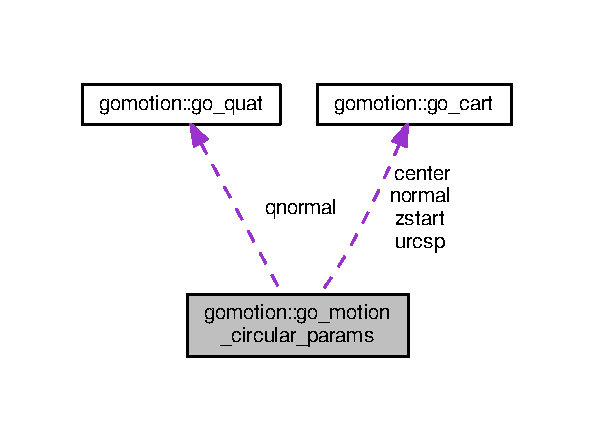
\includegraphics[width=285pt]{da/d58/structgomotion_1_1go__motion__circular__params__coll__graph}
\end{center}
\end{figure}
\subsection*{Data Fields}
\begin{DoxyCompactItemize}
\item 
\hyperlink{structgomotion_1_1go__cart}{go\-\_\-cart} \hyperlink{structgomotion_1_1go__motion__circular__params_afcf8dda6a72f29ce49a61130adbf3971}{center}
\item 
\hyperlink{structgomotion_1_1go__cart}{go\-\_\-cart} \hyperlink{structgomotion_1_1go__motion__circular__params_af933e19d1dba3641d570a3aa42b9969b}{normal}
\item 
\hyperlink{structgomotion_1_1go__quat}{go\-\_\-quat} \hyperlink{structgomotion_1_1go__motion__circular__params_abd5283624621e9fb218671e9996eb3c3}{qnormal}
\item 
\hyperlink{structgomotion_1_1go__cart}{go\-\_\-cart} \hyperlink{structgomotion_1_1go__motion__circular__params_ab97f8ccebf3ca78e2be4a4adfe9c9e8c}{urcsp}
\item 
\hyperlink{gotypes_8h_afd666a2393eebd71ee455846ac9def9b}{go\-\_\-real} \hyperlink{structgomotion_1_1go__motion__circular__params_aeee40430ac2667fef1fc6eba842427b7}{rstart}
\item 
\hyperlink{structgomotion_1_1go__cart}{go\-\_\-cart} \hyperlink{structgomotion_1_1go__motion__circular__params_a3638d197aac3d27862052befae408e94}{zstart}
\item 
\hyperlink{gotypes_8h_afd666a2393eebd71ee455846ac9def9b}{go\-\_\-real} \hyperlink{structgomotion_1_1go__motion__circular__params_a03f65f0ef19c2d9e83d05de75fe9fd3f}{thtot}
\item 
\hyperlink{gotypes_8h_afd666a2393eebd71ee455846ac9def9b}{go\-\_\-real} \hyperlink{structgomotion_1_1go__motion__circular__params_a576992f878d73c0771e072fe37438f4f}{rtot}
\item 
\hyperlink{gotypes_8h_afd666a2393eebd71ee455846ac9def9b}{go\-\_\-real} \hyperlink{structgomotion_1_1go__motion__circular__params_a1572625c5322b3ace560429703948191}{ztot}
\item 
\hyperlink{gotypes_8h_afd666a2393eebd71ee455846ac9def9b}{go\-\_\-real} \hyperlink{structgomotion_1_1go__motion__circular__params_a4436b498d123ce3776166eb75e8efcd5}{stotinv}
\item 
\hyperlink{gotypes_8h_a7d30f606bb0f58ffe2b3bd71e5c8af5c}{go\-\_\-integer} \hyperlink{structgomotion_1_1go__motion__circular__params_a2d8430003302e61cb95c2a0c75e60037}{turns}
\end{DoxyCompactItemize}


\subsection{Field Documentation}
\hypertarget{structgomotion_1_1go__motion__circular__params_afcf8dda6a72f29ce49a61130adbf3971}{\index{gomotion\-::go\-\_\-motion\-\_\-circular\-\_\-params@{gomotion\-::go\-\_\-motion\-\_\-circular\-\_\-params}!center@{center}}
\index{center@{center}!gomotion::go_motion_circular_params@{gomotion\-::go\-\_\-motion\-\_\-circular\-\_\-params}}
\subsubsection[{center}]{\setlength{\rightskip}{0pt plus 5cm}{\bf go\-\_\-cart} gomotion\-::go\-\_\-motion\-\_\-circular\-\_\-params\-::center}}\label{structgomotion_1_1go__motion__circular__params_afcf8dda6a72f29ce49a61130adbf3971}
The vector to the circle center. \hypertarget{structgomotion_1_1go__motion__circular__params_af933e19d1dba3641d570a3aa42b9969b}{\index{gomotion\-::go\-\_\-motion\-\_\-circular\-\_\-params@{gomotion\-::go\-\_\-motion\-\_\-circular\-\_\-params}!normal@{normal}}
\index{normal@{normal}!gomotion::go_motion_circular_params@{gomotion\-::go\-\_\-motion\-\_\-circular\-\_\-params}}
\subsubsection[{normal}]{\setlength{\rightskip}{0pt plus 5cm}{\bf go\-\_\-cart} gomotion\-::go\-\_\-motion\-\_\-circular\-\_\-params\-::normal}}\label{structgomotion_1_1go__motion__circular__params_af933e19d1dba3641d570a3aa42b9969b}
The normal vector that defines the plane of the circle. \hypertarget{structgomotion_1_1go__motion__circular__params_abd5283624621e9fb218671e9996eb3c3}{\index{gomotion\-::go\-\_\-motion\-\_\-circular\-\_\-params@{gomotion\-::go\-\_\-motion\-\_\-circular\-\_\-params}!qnormal@{qnormal}}
\index{qnormal@{qnormal}!gomotion::go_motion_circular_params@{gomotion\-::go\-\_\-motion\-\_\-circular\-\_\-params}}
\subsubsection[{qnormal}]{\setlength{\rightskip}{0pt plus 5cm}{\bf go\-\_\-quat} gomotion\-::go\-\_\-motion\-\_\-circular\-\_\-params\-::qnormal}}\label{structgomotion_1_1go__motion__circular__params_abd5283624621e9fb218671e9996eb3c3}
The normal vector expressed as a unit rotation. \hypertarget{structgomotion_1_1go__motion__circular__params_aeee40430ac2667fef1fc6eba842427b7}{\index{gomotion\-::go\-\_\-motion\-\_\-circular\-\_\-params@{gomotion\-::go\-\_\-motion\-\_\-circular\-\_\-params}!rstart@{rstart}}
\index{rstart@{rstart}!gomotion::go_motion_circular_params@{gomotion\-::go\-\_\-motion\-\_\-circular\-\_\-params}}
\subsubsection[{rstart}]{\setlength{\rightskip}{0pt plus 5cm}{\bf go\-\_\-real} gomotion\-::go\-\_\-motion\-\_\-circular\-\_\-params\-::rstart}}\label{structgomotion_1_1go__motion__circular__params_aeee40430ac2667fef1fc6eba842427b7}
The starting radius. \hypertarget{structgomotion_1_1go__motion__circular__params_a576992f878d73c0771e072fe37438f4f}{\index{gomotion\-::go\-\_\-motion\-\_\-circular\-\_\-params@{gomotion\-::go\-\_\-motion\-\_\-circular\-\_\-params}!rtot@{rtot}}
\index{rtot@{rtot}!gomotion::go_motion_circular_params@{gomotion\-::go\-\_\-motion\-\_\-circular\-\_\-params}}
\subsubsection[{rtot}]{\setlength{\rightskip}{0pt plus 5cm}{\bf go\-\_\-real} gomotion\-::go\-\_\-motion\-\_\-circular\-\_\-params\-::rtot}}\label{structgomotion_1_1go__motion__circular__params_a576992f878d73c0771e072fe37438f4f}
The signed displacement from start to end projected radii \hypertarget{structgomotion_1_1go__motion__circular__params_a4436b498d123ce3776166eb75e8efcd5}{\index{gomotion\-::go\-\_\-motion\-\_\-circular\-\_\-params@{gomotion\-::go\-\_\-motion\-\_\-circular\-\_\-params}!stotinv@{stotinv}}
\index{stotinv@{stotinv}!gomotion::go_motion_circular_params@{gomotion\-::go\-\_\-motion\-\_\-circular\-\_\-params}}
\subsubsection[{stotinv}]{\setlength{\rightskip}{0pt plus 5cm}{\bf go\-\_\-real} gomotion\-::go\-\_\-motion\-\_\-circular\-\_\-params\-::stotinv}}\label{structgomotion_1_1go__motion__circular__params_a4436b498d123ce3776166eb75e8efcd5}
The inverse of total approximate arc length. If negative, no translation motion is taking place. \hypertarget{structgomotion_1_1go__motion__circular__params_a03f65f0ef19c2d9e83d05de75fe9fd3f}{\index{gomotion\-::go\-\_\-motion\-\_\-circular\-\_\-params@{gomotion\-::go\-\_\-motion\-\_\-circular\-\_\-params}!thtot@{thtot}}
\index{thtot@{thtot}!gomotion::go_motion_circular_params@{gomotion\-::go\-\_\-motion\-\_\-circular\-\_\-params}}
\subsubsection[{thtot}]{\setlength{\rightskip}{0pt plus 5cm}{\bf go\-\_\-real} gomotion\-::go\-\_\-motion\-\_\-circular\-\_\-params\-::thtot}}\label{structgomotion_1_1go__motion__circular__params_a03f65f0ef19c2d9e83d05de75fe9fd3f}
The signed total angular displacement around normal vector \hypertarget{structgomotion_1_1go__motion__circular__params_a2d8430003302e61cb95c2a0c75e60037}{\index{gomotion\-::go\-\_\-motion\-\_\-circular\-\_\-params@{gomotion\-::go\-\_\-motion\-\_\-circular\-\_\-params}!turns@{turns}}
\index{turns@{turns}!gomotion::go_motion_circular_params@{gomotion\-::go\-\_\-motion\-\_\-circular\-\_\-params}}
\subsubsection[{turns}]{\setlength{\rightskip}{0pt plus 5cm}{\bf go\-\_\-integer} gomotion\-::go\-\_\-motion\-\_\-circular\-\_\-params\-::turns}}\label{structgomotion_1_1go__motion__circular__params_a2d8430003302e61cb95c2a0c75e60037}
The number of turns in the circle. 0 means partial C\-C\-W, -\/1 means partial C\-W, otherwise more turns are added in each direction. \hypertarget{structgomotion_1_1go__motion__circular__params_ab97f8ccebf3ca78e2be4a4adfe9c9e8c}{\index{gomotion\-::go\-\_\-motion\-\_\-circular\-\_\-params@{gomotion\-::go\-\_\-motion\-\_\-circular\-\_\-params}!urcsp@{urcsp}}
\index{urcsp@{urcsp}!gomotion::go_motion_circular_params@{gomotion\-::go\-\_\-motion\-\_\-circular\-\_\-params}}
\subsubsection[{urcsp}]{\setlength{\rightskip}{0pt plus 5cm}{\bf go\-\_\-cart} gomotion\-::go\-\_\-motion\-\_\-circular\-\_\-params\-::urcsp}}\label{structgomotion_1_1go__motion__circular__params_ab97f8ccebf3ca78e2be4a4adfe9c9e8c}
The unit vector from center to start, projected onto the normal plane. \hypertarget{structgomotion_1_1go__motion__circular__params_a3638d197aac3d27862052befae408e94}{\index{gomotion\-::go\-\_\-motion\-\_\-circular\-\_\-params@{gomotion\-::go\-\_\-motion\-\_\-circular\-\_\-params}!zstart@{zstart}}
\index{zstart@{zstart}!gomotion::go_motion_circular_params@{gomotion\-::go\-\_\-motion\-\_\-circular\-\_\-params}}
\subsubsection[{zstart}]{\setlength{\rightskip}{0pt plus 5cm}{\bf go\-\_\-cart} gomotion\-::go\-\_\-motion\-\_\-circular\-\_\-params\-::zstart}}\label{structgomotion_1_1go__motion__circular__params_a3638d197aac3d27862052befae408e94}
The vector from the normal plane to the start. \hypertarget{structgomotion_1_1go__motion__circular__params_a1572625c5322b3ace560429703948191}{\index{gomotion\-::go\-\_\-motion\-\_\-circular\-\_\-params@{gomotion\-::go\-\_\-motion\-\_\-circular\-\_\-params}!ztot@{ztot}}
\index{ztot@{ztot}!gomotion::go_motion_circular_params@{gomotion\-::go\-\_\-motion\-\_\-circular\-\_\-params}}
\subsubsection[{ztot}]{\setlength{\rightskip}{0pt plus 5cm}{\bf go\-\_\-real} gomotion\-::go\-\_\-motion\-\_\-circular\-\_\-params\-::ztot}}\label{structgomotion_1_1go__motion__circular__params_a1572625c5322b3ace560429703948191}
The signed displacement from start to end z off-\/normals 

The documentation for this struct was generated from the following file\-:\begin{DoxyCompactItemize}
\item 
/usr/local/michalos/nistfanuc\-\_\-ws/src/gomotion/include/gomotion/\hyperlink{gomotion_8h}{gomotion.\-h}\end{DoxyCompactItemize}

\hypertarget{structgomotion_1_1go__motion__interface}{\section{gomotion\-:\-:go\-\_\-motion\-\_\-interface Struct Reference}
\label{structgomotion_1_1go__motion__interface}\index{gomotion\-::go\-\_\-motion\-\_\-interface@{gomotion\-::go\-\_\-motion\-\_\-interface}}
}


Collaboration diagram for gomotion\-:\-:go\-\_\-motion\-\_\-interface\-:\nopagebreak
\begin{figure}[H]
\begin{center}
\leavevmode
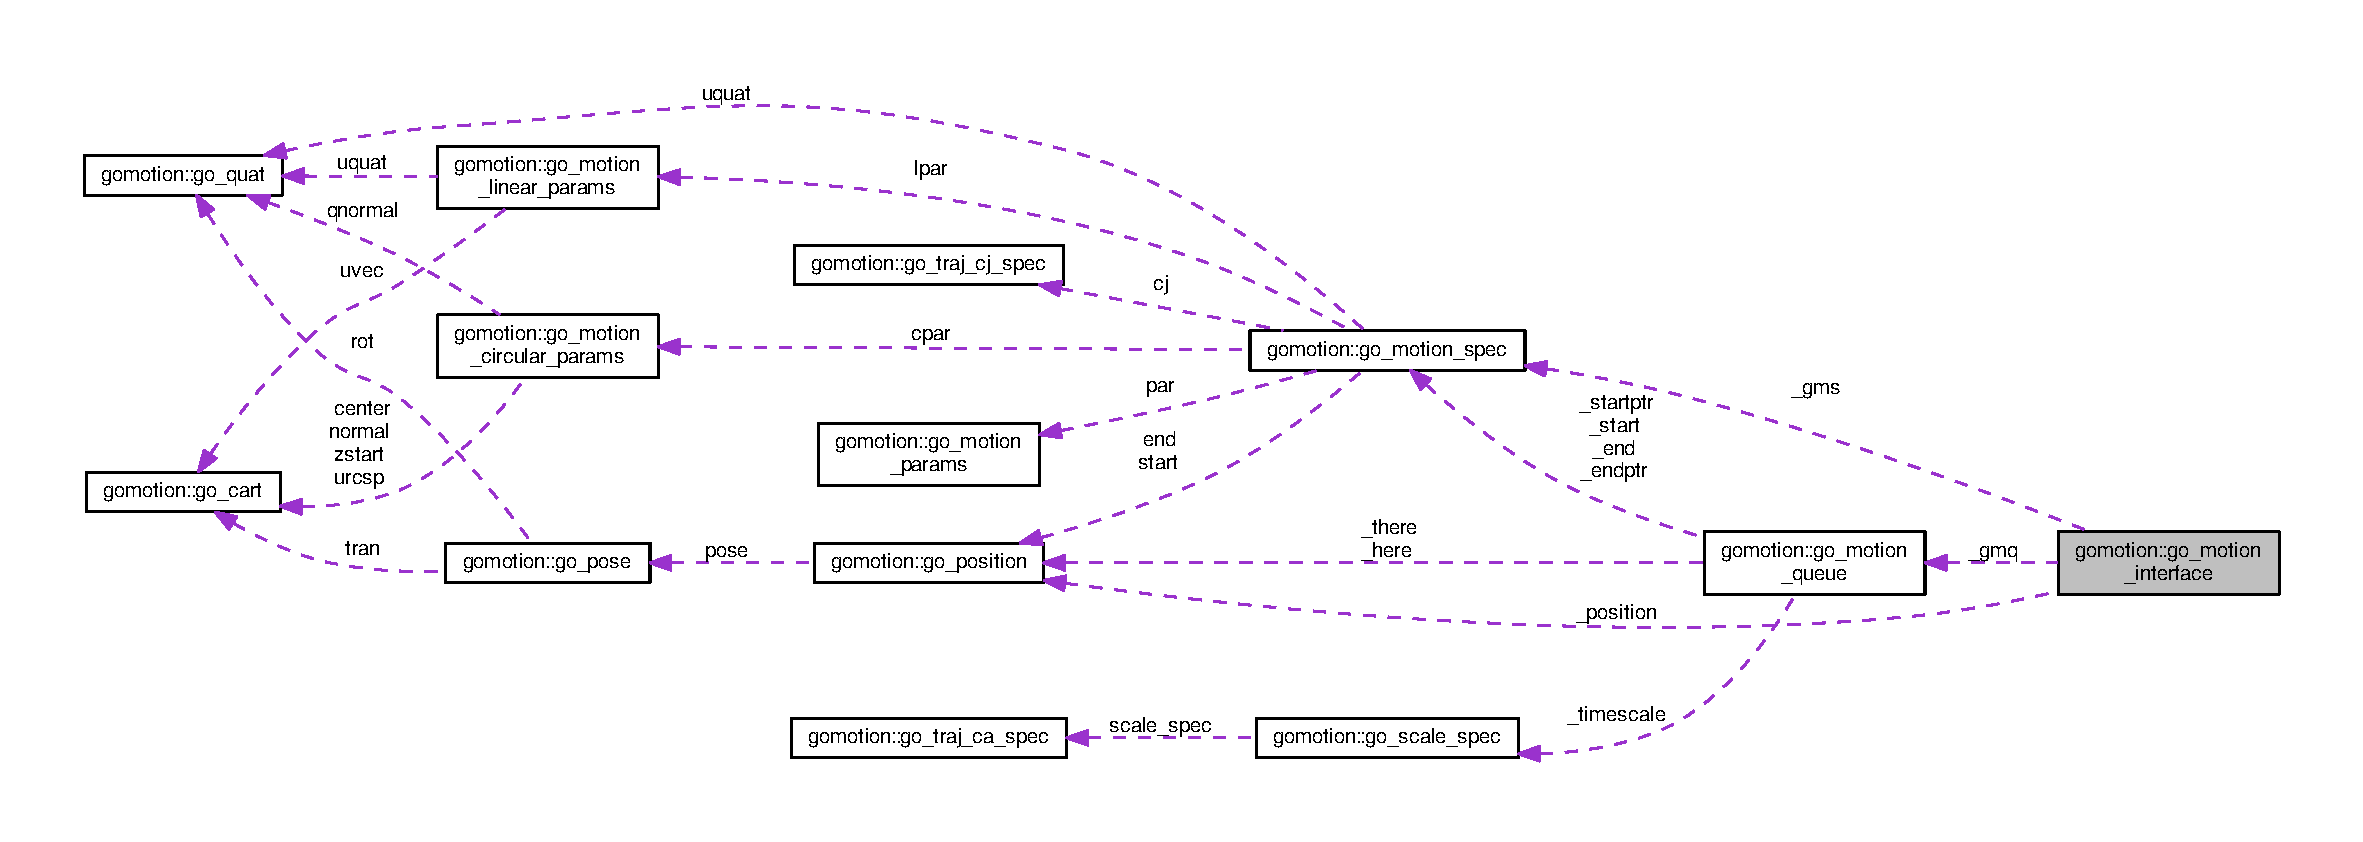
\includegraphics[width=350pt]{d3/d89/structgomotion_1_1go__motion__interface__coll__graph}
\end{center}
\end{figure}
\subsection*{Data Fields}
\begin{DoxyCompactItemize}
\item 
int \hyperlink{structgomotion_1_1go__motion__interface_a10ef45dfc2f8c62e518fb23bacef0fda}{\-\_\-type}
\item 
double \hyperlink{structgomotion_1_1go__motion__interface_a450ed54375d304ec8e2b00be571f7fb2}{\-\_\-deltat}
\item 
\hyperlink{structgomotion_1_1go__motion__spec}{go\-\_\-motion\-\_\-spec} \hyperlink{structgomotion_1_1go__motion__interface_a027cf7ca47ea59b2ce242a9ada705ea5}{\-\_\-gms}
\item 
std\-::vector$<$ \hyperlink{structgomotion_1_1go__motion__spec}{go\-\_\-motion\-\_\-spec} $>$ \hyperlink{structgomotion_1_1go__motion__interface_a9de0b8636128c1107ce815c5e44a9c28}{\-\_\-space}
\item 
\hyperlink{structgomotion_1_1go__motion__queue}{go\-\_\-motion\-\_\-queue} \hyperlink{structgomotion_1_1go__motion__interface_ab7801d0e1621e18025d2a3446648ac5e}{\-\_\-gmq}
\item 
\hyperlink{structgomotion_1_1go__position}{go\-\_\-position} \hyperlink{structgomotion_1_1go__motion__interface_a1da77c6de12dd3b2714bb55ebe041924}{\-\_\-position}
\item 
size\-\_\-t \hyperlink{structgomotion_1_1go__motion__interface_a26585b0cd74b71796be70d71ac6c2b63}{\-\_\-queuesize}
\end{DoxyCompactItemize}
\subsection*{Static Public Attributes}
\begin{DoxyCompactItemize}
\item 
static size\-\_\-t \hyperlink{structgomotion_1_1go__motion__interface_aba0811a381c6f1a25fa0f68dfde0b829}{\-\_\-id} = 0
\end{DoxyCompactItemize}


\subsection{Field Documentation}
\hypertarget{structgomotion_1_1go__motion__interface_a450ed54375d304ec8e2b00be571f7fb2}{\index{gomotion\-::go\-\_\-motion\-\_\-interface@{gomotion\-::go\-\_\-motion\-\_\-interface}!\-\_\-deltat@{\-\_\-deltat}}
\index{\-\_\-deltat@{\-\_\-deltat}!gomotion::go_motion_interface@{gomotion\-::go\-\_\-motion\-\_\-interface}}
\subsubsection[{\-\_\-deltat}]{\setlength{\rightskip}{0pt plus 5cm}double gomotion\-::go\-\_\-motion\-\_\-interface\-::\-\_\-deltat}}\label{structgomotion_1_1go__motion__interface_a450ed54375d304ec8e2b00be571f7fb2}
\hypertarget{structgomotion_1_1go__motion__interface_ab7801d0e1621e18025d2a3446648ac5e}{\index{gomotion\-::go\-\_\-motion\-\_\-interface@{gomotion\-::go\-\_\-motion\-\_\-interface}!\-\_\-gmq@{\-\_\-gmq}}
\index{\-\_\-gmq@{\-\_\-gmq}!gomotion::go_motion_interface@{gomotion\-::go\-\_\-motion\-\_\-interface}}
\subsubsection[{\-\_\-gmq}]{\setlength{\rightskip}{0pt plus 5cm}{\bf go\-\_\-motion\-\_\-queue} gomotion\-::go\-\_\-motion\-\_\-interface\-::\-\_\-gmq}}\label{structgomotion_1_1go__motion__interface_ab7801d0e1621e18025d2a3446648ac5e}
\hypertarget{structgomotion_1_1go__motion__interface_a027cf7ca47ea59b2ce242a9ada705ea5}{\index{gomotion\-::go\-\_\-motion\-\_\-interface@{gomotion\-::go\-\_\-motion\-\_\-interface}!\-\_\-gms@{\-\_\-gms}}
\index{\-\_\-gms@{\-\_\-gms}!gomotion::go_motion_interface@{gomotion\-::go\-\_\-motion\-\_\-interface}}
\subsubsection[{\-\_\-gms}]{\setlength{\rightskip}{0pt plus 5cm}{\bf go\-\_\-motion\-\_\-spec} gomotion\-::go\-\_\-motion\-\_\-interface\-::\-\_\-gms}}\label{structgomotion_1_1go__motion__interface_a027cf7ca47ea59b2ce242a9ada705ea5}
\hypertarget{structgomotion_1_1go__motion__interface_aba0811a381c6f1a25fa0f68dfde0b829}{\index{gomotion\-::go\-\_\-motion\-\_\-interface@{gomotion\-::go\-\_\-motion\-\_\-interface}!\-\_\-id@{\-\_\-id}}
\index{\-\_\-id@{\-\_\-id}!gomotion::go_motion_interface@{gomotion\-::go\-\_\-motion\-\_\-interface}}
\subsubsection[{\-\_\-id}]{\setlength{\rightskip}{0pt plus 5cm}size\-\_\-t gomotion\-::go\-\_\-motion\-\_\-interface\-::\-\_\-id = 0\hspace{0.3cm}{\ttfamily [static]}}}\label{structgomotion_1_1go__motion__interface_aba0811a381c6f1a25fa0f68dfde0b829}
\hypertarget{structgomotion_1_1go__motion__interface_a1da77c6de12dd3b2714bb55ebe041924}{\index{gomotion\-::go\-\_\-motion\-\_\-interface@{gomotion\-::go\-\_\-motion\-\_\-interface}!\-\_\-position@{\-\_\-position}}
\index{\-\_\-position@{\-\_\-position}!gomotion::go_motion_interface@{gomotion\-::go\-\_\-motion\-\_\-interface}}
\subsubsection[{\-\_\-position}]{\setlength{\rightskip}{0pt plus 5cm}{\bf go\-\_\-position} gomotion\-::go\-\_\-motion\-\_\-interface\-::\-\_\-position}}\label{structgomotion_1_1go__motion__interface_a1da77c6de12dd3b2714bb55ebe041924}
\hypertarget{structgomotion_1_1go__motion__interface_a26585b0cd74b71796be70d71ac6c2b63}{\index{gomotion\-::go\-\_\-motion\-\_\-interface@{gomotion\-::go\-\_\-motion\-\_\-interface}!\-\_\-queuesize@{\-\_\-queuesize}}
\index{\-\_\-queuesize@{\-\_\-queuesize}!gomotion::go_motion_interface@{gomotion\-::go\-\_\-motion\-\_\-interface}}
\subsubsection[{\-\_\-queuesize}]{\setlength{\rightskip}{0pt plus 5cm}size\-\_\-t gomotion\-::go\-\_\-motion\-\_\-interface\-::\-\_\-queuesize}}\label{structgomotion_1_1go__motion__interface_a26585b0cd74b71796be70d71ac6c2b63}
\hypertarget{structgomotion_1_1go__motion__interface_a9de0b8636128c1107ce815c5e44a9c28}{\index{gomotion\-::go\-\_\-motion\-\_\-interface@{gomotion\-::go\-\_\-motion\-\_\-interface}!\-\_\-space@{\-\_\-space}}
\index{\-\_\-space@{\-\_\-space}!gomotion::go_motion_interface@{gomotion\-::go\-\_\-motion\-\_\-interface}}
\subsubsection[{\-\_\-space}]{\setlength{\rightskip}{0pt plus 5cm}std\-::vector$<${\bf go\-\_\-motion\-\_\-spec}$>$ gomotion\-::go\-\_\-motion\-\_\-interface\-::\-\_\-space}}\label{structgomotion_1_1go__motion__interface_a9de0b8636128c1107ce815c5e44a9c28}
\hypertarget{structgomotion_1_1go__motion__interface_a10ef45dfc2f8c62e518fb23bacef0fda}{\index{gomotion\-::go\-\_\-motion\-\_\-interface@{gomotion\-::go\-\_\-motion\-\_\-interface}!\-\_\-type@{\-\_\-type}}
\index{\-\_\-type@{\-\_\-type}!gomotion::go_motion_interface@{gomotion\-::go\-\_\-motion\-\_\-interface}}
\subsubsection[{\-\_\-type}]{\setlength{\rightskip}{0pt plus 5cm}int gomotion\-::go\-\_\-motion\-\_\-interface\-::\-\_\-type}}\label{structgomotion_1_1go__motion__interface_a10ef45dfc2f8c62e518fb23bacef0fda}


The documentation for this struct was generated from the following file\-:\begin{DoxyCompactItemize}
\item 
/usr/local/michalos/nistfanuc\-\_\-ws/src/gomotion/src/\hyperlink{gomove_8cpp}{gomove.\-cpp}\end{DoxyCompactItemize}

\hypertarget{structgomotion_1_1go__motion__linear__params}{\section{gomotion\-:\-:go\-\_\-motion\-\_\-linear\-\_\-params Struct Reference}
\label{structgomotion_1_1go__motion__linear__params}\index{gomotion\-::go\-\_\-motion\-\_\-linear\-\_\-params@{gomotion\-::go\-\_\-motion\-\_\-linear\-\_\-params}}
}


In the following comments, L\-I\-N, C\-I\-R and A\-L\-L refer to linear moves, circular moves and both, respectively.  




{\ttfamily \#include $<$gomotion.\-h$>$}



Collaboration diagram for gomotion\-:\-:go\-\_\-motion\-\_\-linear\-\_\-params\-:\nopagebreak
\begin{figure}[H]
\begin{center}
\leavevmode
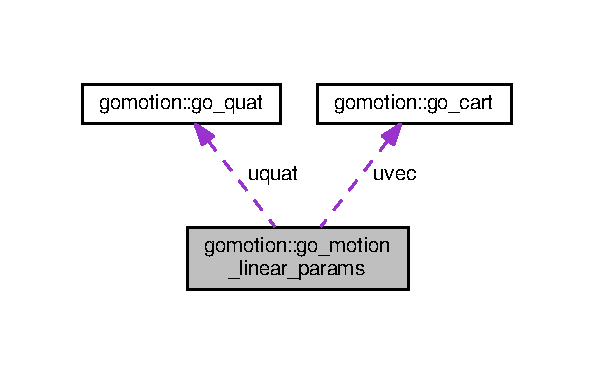
\includegraphics[width=285pt]{d6/dbf/structgomotion_1_1go__motion__linear__params__coll__graph}
\end{center}
\end{figure}
\subsection*{Data Fields}
\begin{DoxyCompactItemize}
\item 
\hyperlink{structgomotion_1_1go__cart}{go\-\_\-cart} \hyperlink{structgomotion_1_1go__motion__linear__params_ab1865f783998b55efb3c97f62e6a4f7d}{uvec}
\item 
\hyperlink{structgomotion_1_1go__quat}{go\-\_\-quat} \hyperlink{structgomotion_1_1go__motion__linear__params_af354e180468997cc31fca9f21a9bc325}{uquat}
\end{DoxyCompactItemize}


\subsection{Detailed Description}
In the following comments, L\-I\-N, C\-I\-R and A\-L\-L refer to linear moves, circular moves and both, respectively. 

If they are not in parens, e.\-g., A\-L\-L\-:, you need to provide them for that type of motion. If they are in parens, e.\-g., (C\-I\-R), they are computed for you. 

\subsection{Field Documentation}
\hypertarget{structgomotion_1_1go__motion__linear__params_af354e180468997cc31fca9f21a9bc325}{\index{gomotion\-::go\-\_\-motion\-\_\-linear\-\_\-params@{gomotion\-::go\-\_\-motion\-\_\-linear\-\_\-params}!uquat@{uquat}}
\index{uquat@{uquat}!gomotion::go_motion_linear_params@{gomotion\-::go\-\_\-motion\-\_\-linear\-\_\-params}}
\subsubsection[{uquat}]{\setlength{\rightskip}{0pt plus 5cm}{\bf go\-\_\-quat} gomotion\-::go\-\_\-motion\-\_\-linear\-\_\-params\-::uquat}}\label{structgomotion_1_1go__motion__linear__params_af354e180468997cc31fca9f21a9bc325}
\hypertarget{structgomotion_1_1go__motion__linear__params_ab1865f783998b55efb3c97f62e6a4f7d}{\index{gomotion\-::go\-\_\-motion\-\_\-linear\-\_\-params@{gomotion\-::go\-\_\-motion\-\_\-linear\-\_\-params}!uvec@{uvec}}
\index{uvec@{uvec}!gomotion::go_motion_linear_params@{gomotion\-::go\-\_\-motion\-\_\-linear\-\_\-params}}
\subsubsection[{uvec}]{\setlength{\rightskip}{0pt plus 5cm}{\bf go\-\_\-cart} gomotion\-::go\-\_\-motion\-\_\-linear\-\_\-params\-::uvec}}\label{structgomotion_1_1go__motion__linear__params_ab1865f783998b55efb3c97f62e6a4f7d}


The documentation for this struct was generated from the following file\-:\begin{DoxyCompactItemize}
\item 
/usr/local/michalos/nistfanuc\-\_\-ws/src/gomotion/include/gomotion/\hyperlink{gomotion_8h}{gomotion.\-h}\end{DoxyCompactItemize}

\hypertarget{structgomotion_1_1go__motion__params}{\section{gomotion\-:\-:go\-\_\-motion\-\_\-params Struct Reference}
\label{structgomotion_1_1go__motion__params}\index{gomotion\-::go\-\_\-motion\-\_\-params@{gomotion\-::go\-\_\-motion\-\_\-params}}
}


{\ttfamily \#include $<$gomotion.\-h$>$}

\subsection*{Data Fields}
\begin{DoxyCompactItemize}
\item 
\hyperlink{gotypes_8h_afd666a2393eebd71ee455846ac9def9b}{go\-\_\-real} \hyperlink{structgomotion_1_1go__motion__params_ad3121c36c5257557895df5d036b22c9d}{vel}
\begin{DoxyCompactList}\small\item\em max vel for each motion \end{DoxyCompactList}\item 
\hyperlink{gotypes_8h_afd666a2393eebd71ee455846ac9def9b}{go\-\_\-real} \hyperlink{structgomotion_1_1go__motion__params_a494815c0bc4016f78b82e2005ee6ad70}{acc}
\begin{DoxyCompactList}\small\item\em max accel for each motion \end{DoxyCompactList}\item 
\hyperlink{gotypes_8h_afd666a2393eebd71ee455846ac9def9b}{go\-\_\-real} \hyperlink{structgomotion_1_1go__motion__params_a25db76d9565efdc899bc8bc28b4a7c32}{jerk}
\begin{DoxyCompactList}\small\item\em max jerk for each motion \end{DoxyCompactList}\end{DoxyCompactItemize}


\subsection{Field Documentation}
\hypertarget{structgomotion_1_1go__motion__params_a494815c0bc4016f78b82e2005ee6ad70}{\index{gomotion\-::go\-\_\-motion\-\_\-params@{gomotion\-::go\-\_\-motion\-\_\-params}!acc@{acc}}
\index{acc@{acc}!gomotion::go_motion_params@{gomotion\-::go\-\_\-motion\-\_\-params}}
\subsubsection[{acc}]{\setlength{\rightskip}{0pt plus 5cm}{\bf go\-\_\-real} gomotion\-::go\-\_\-motion\-\_\-params\-::acc}}\label{structgomotion_1_1go__motion__params_a494815c0bc4016f78b82e2005ee6ad70}


max accel for each motion 

\hypertarget{structgomotion_1_1go__motion__params_a25db76d9565efdc899bc8bc28b4a7c32}{\index{gomotion\-::go\-\_\-motion\-\_\-params@{gomotion\-::go\-\_\-motion\-\_\-params}!jerk@{jerk}}
\index{jerk@{jerk}!gomotion::go_motion_params@{gomotion\-::go\-\_\-motion\-\_\-params}}
\subsubsection[{jerk}]{\setlength{\rightskip}{0pt plus 5cm}{\bf go\-\_\-real} gomotion\-::go\-\_\-motion\-\_\-params\-::jerk}}\label{structgomotion_1_1go__motion__params_a25db76d9565efdc899bc8bc28b4a7c32}


max jerk for each motion 

\hypertarget{structgomotion_1_1go__motion__params_ad3121c36c5257557895df5d036b22c9d}{\index{gomotion\-::go\-\_\-motion\-\_\-params@{gomotion\-::go\-\_\-motion\-\_\-params}!vel@{vel}}
\index{vel@{vel}!gomotion::go_motion_params@{gomotion\-::go\-\_\-motion\-\_\-params}}
\subsubsection[{vel}]{\setlength{\rightskip}{0pt plus 5cm}{\bf go\-\_\-real} gomotion\-::go\-\_\-motion\-\_\-params\-::vel}}\label{structgomotion_1_1go__motion__params_ad3121c36c5257557895df5d036b22c9d}


max vel for each motion 



The documentation for this struct was generated from the following file\-:\begin{DoxyCompactItemize}
\item 
/usr/local/michalos/nistfanuc\-\_\-ws/src/gomotion/include/gomotion/\hyperlink{gomotion_8h}{gomotion.\-h}\end{DoxyCompactItemize}

\hypertarget{structgomotion_1_1go__motion__queue}{\section{gomotion\-:\-:go\-\_\-motion\-\_\-queue Struct Reference}
\label{structgomotion_1_1go__motion__queue}\index{gomotion\-::go\-\_\-motion\-\_\-queue@{gomotion\-::go\-\_\-motion\-\_\-queue}}
}
\subsection*{Public Member Functions}
\begin{DoxyCompactItemize}
\item 
\hypertarget{structgomotion_1_1go__motion__queue_a23b5be5b838cf78eff17f8a7fa5df490}{go\-\_\-result {\bfseries init} (\hyperlink{structgomotion_1_1go__motion__spec}{go\-\_\-motion\-\_\-spec} $\ast$space, go\-\_\-integer size, go\-\_\-real deltat)}\label{structgomotion_1_1go__motion__queue_a23b5be5b838cf78eff17f8a7fa5df490}

\item 
go\-\_\-result \hyperlink{structgomotion_1_1go__motion__queue_a2eb9870461c0c071b2576c0071aebae7}{reset} ()
\begin{DoxyCompactList}\small\item\em Reset motion queue. Null motion type, reset start and set end to start, Zero number of motions on queue, last\-\_\-id of motion on queue, time. Init timescale to 1.\-0. \end{DoxyCompactList}\item 
go\-\_\-result \hyperlink{structgomotion_1_1go__motion__queue_a7ecc32334fd878989a9c1aba2dd8f309}{set\-\_\-type} (go\-\_\-flag type)
\begin{DoxyCompactList}\small\item\em Set type of motion queueing done\-: G\-O\-\_\-\-M\-O\-T\-I\-O\-N\-\_\-\-N\-O\-N\-E, G\-O\-\_\-\-M\-O\-T\-I\-O\-N\-\_\-\-J\-O\-I\-N\-T, G\-O\-\_\-\-M\-O\-T\-I\-O\-N\-\_\-\-U\-J\-O\-I\-N\-T, G\-O\-\_\-\-M\-O\-T\-I\-O\-N\-\_\-\-W\-O\-R\-L\-D. \end{DoxyCompactList}\item 
\hypertarget{structgomotion_1_1go__motion__queue_a29775f13e13d7ca216e416c87b14fcdb}{go\-\_\-flag {\bfseries get\-\_\-type} ()}\label{structgomotion_1_1go__motion__queue_a29775f13e13d7ca216e416c87b14fcdb}

\item 
go\-\_\-result \hyperlink{structgomotion_1_1go__motion__queue_ac623c003c01542bea2151f38b622c67e}{set\-\_\-joint\-\_\-number} (go\-\_\-integer joints)
\begin{DoxyCompactList}\small\item\em Set number of joints. Must positive andless than G\-O\-\_\-\-M\-O\-T\-I\-O\-N\-\_\-\-J\-O\-I\-N\-T\-\_\-\-N\-U\-M. \end{DoxyCompactList}\item 
go\-\_\-integer \hyperlink{structgomotion_1_1go__motion__queue_ac2fcc83c90ccd7794d7407174eaf2b37}{get\-\_\-joint\-\_\-number} ()
\begin{DoxyCompactList}\small\item\em Get number of joints. \end{DoxyCompactList}\item 
go\-\_\-result \hyperlink{structgomotion_1_1go__motion__queue_a0580645d22f2db0893ccd1cc0271469d}{set\-\_\-here} (const \hyperlink{structgomotion_1_1go__position}{go\-\_\-position} $\ast$\hyperlink{structgomotion_1_1go__motion__queue_ab45a3644aac5d496e758db38a3553037}{here})
\begin{DoxyCompactList}\small\item\em Set current position -\/ either joint values or world Cartesian pose. \end{DoxyCompactList}\item 
go\-\_\-result \hyperlink{structgomotion_1_1go__motion__queue_a560b24166fe53f8e2d8be6afaf08c7e9}{set\-\_\-cycle\-\_\-time} (go\-\_\-real deltat)
\begin{DoxyCompactList}\small\item\em Set deltat, the time in seconds per cycle. \end{DoxyCompactList}\item 
\hypertarget{structgomotion_1_1go__motion__queue_addfc802fee86a93050de27d185c4030b}{go\-\_\-result {\bfseries set\-\_\-scale} (go\-\_\-real scale, go\-\_\-real scale\-\_\-v, go\-\_\-real scale\-\_\-a)}\label{structgomotion_1_1go__motion__queue_addfc802fee86a93050de27d185c4030b}

\item 
go\-\_\-result \hyperlink{structgomotion_1_1go__motion__queue_aed6b10eacd99af71b2b0cf69d6ddebeb}{append} (const \hyperlink{structgomotion_1_1go__motion__spec}{go\-\_\-motion\-\_\-spec} $\ast$motion)
\begin{DoxyCompactList}\small\item\em Append motion\-\_\-spec onto queue. if type is G\-O\-\_\-\-M\-O\-T\-I\-O\-N\-\_\-\-J\-O\-I\-N\-T then motion is done as append\-\_\-joint if type is G\-O\-\_\-\-M\-O\-T\-I\-O\-N\-\_\-\-U\-J\-O\-I\-N\-T then motion is done as append\-\_\-ujoint if type is G\-O\-\_\-\-M\-O\-T\-I\-O\-N\-\_\-\-W\-O\-R\-L\-D then motion is done as append\-\_\-world. \end{DoxyCompactList}\item 
\hypertarget{structgomotion_1_1go__motion__queue_a8dfbc19656f2dfcf1e99c27e6a909c4d}{go\-\_\-result {\bfseries number} (go\-\_\-integer $\ast$number)}\label{structgomotion_1_1go__motion__queue_a8dfbc19656f2dfcf1e99c27e6a909c4d}

\item 
\hypertarget{structgomotion_1_1go__motion__queue_a9eb929528abd0d19d272110c67236dce}{go\-\_\-result {\bfseries size} (go\-\_\-integer $\ast$size)}\label{structgomotion_1_1go__motion__queue_a9eb929528abd0d19d272110c67236dce}

\item 
go\-\_\-result \hyperlink{structgomotion_1_1go__motion__queue_a3fe40223c4ad5a19b929b192d7cead64}{head} (\hyperlink{structgomotion_1_1go__motion__spec}{go\-\_\-motion\-\_\-spec} $\ast$motion)
\begin{DoxyCompactList}\small\item\em Get the head of the motion queue. \end{DoxyCompactList}\item 
go\-\_\-result \hyperlink{structgomotion_1_1go__motion__queue_ab45a3644aac5d496e758db38a3553037}{here} (\hyperlink{structgomotion_1_1go__position}{go\-\_\-position} $\ast$position)
\begin{DoxyCompactList}\small\item\em Get the here position and store into pointer to \hyperlink{structgomotion_1_1go__motion__spec}{go\-\_\-motion\-\_\-spec}. \end{DoxyCompactList}\item 
go\-\_\-result \hyperlink{structgomotion_1_1go__motion__queue_ad5de56ac17a7e86ea66627376b668bd2}{there} (\hyperlink{structgomotion_1_1go__position}{go\-\_\-position} $\ast$position)
\begin{DoxyCompactList}\small\item\em Get the there position and store into the motion pointer to \hyperlink{structgomotion_1_1go__motion__spec}{go\-\_\-motion\-\_\-spec}. \end{DoxyCompactList}\item 
go\-\_\-result \hyperlink{structgomotion_1_1go__motion__queue_a3cfb410e307b2bd3af0c64406364edfc}{interp} (\hyperlink{structgomotion_1_1go__position}{go\-\_\-position} $\ast$position)
\begin{DoxyCompactList}\small\item\em Do interpret cycle and store result into position pointer. Only if there's something on the queue do we want to increment the queue time. It was set to 0 when the queue was emptied, and will not be set to zero when the next move is appended. \end{DoxyCompactList}\item 
\hypertarget{structgomotion_1_1go__motion__queue_a59932f32a219889d188e2b4184b396c2}{go\-\_\-result {\bfseries stop} (\hyperlink{structgomotion_1_1go__motion__queue}{go\-\_\-motion\-\_\-queue} $\ast$queue)}\label{structgomotion_1_1go__motion__queue_a59932f32a219889d188e2b4184b396c2}

\item 
go\-\_\-result \hyperlink{structgomotion_1_1go__motion__queue_a10c28cd42c87403852354d8a26e11204}{set\-\_\-id} (go\-\_\-integer id)
\begin{DoxyCompactList}\small\item\em Set id of last motion appended. \end{DoxyCompactList}\item 
go\-\_\-integer \hyperlink{structgomotion_1_1go__motion__queue_ab6be3f8589b1ed1d0cf9615c16d3f7cd}{last\-\_\-id} ()
\begin{DoxyCompactList}\small\item\em Get id of last motion appended. \end{DoxyCompactList}\item 
\hypertarget{structgomotion_1_1go__motion__queue_ad159c5ff1a51e68707caf4c6466da2cb}{go\-\_\-flag {\bfseries is\-\_\-empty} ()}\label{structgomotion_1_1go__motion__queue_ad159c5ff1a51e68707caf4c6466da2cb}

\item 
\hypertarget{structgomotion_1_1go__motion__queue_a0f48a4983551ffa4d5e53e3c62a965c6}{go\-\_\-result {\bfseries erase} ()}\label{structgomotion_1_1go__motion__queue_a0f48a4983551ffa4d5e53e3c62a965c6}

\item 
\hypertarget{structgomotion_1_1go__motion__queue_ac14fbfab39c746da1969390c50617746}{go\-\_\-result {\bfseries drop\-\_\-pending} ()}\label{structgomotion_1_1go__motion__queue_ac14fbfab39c746da1969390c50617746}

\item 
go\-\_\-result \hyperlink{structgomotion_1_1go__motion__queue_ad2fa3a736879c90c0ffbdf7bc0bc54c9}{stop} ()
\begin{DoxyCompactList}\small\item\em Stop queue interpret cycle now. Don't need to stop an empty or stopping queue store computed joint/world motion. point our attention at the current motion. Call go\-\_\-traj\-\_\-cj\-\_\-stop for each joint-\/ or tran/rot motion, so that each stops as fast as it can. The longest to stop will set the revised stop time, and each will be extended to stop at that longest time. Note that the specptr values are incremental for the move, as the original distance passed to go\-\_\-traj\-\_\-cj\-\_\-compute was the incremental distance. \end{DoxyCompactList}\end{DoxyCompactItemize}
\subsection*{Protected Member Functions}
\begin{DoxyCompactItemize}
\item 
\hypertarget{structgomotion_1_1go__motion__queue_a8530405c3ab2eb49c99b78804af3110f}{go\-\_\-result {\bfseries append\-\_\-joint} (const \hyperlink{structgomotion_1_1go__motion__spec}{go\-\_\-motion\-\_\-spec} $\ast$motion)}\label{structgomotion_1_1go__motion__queue_a8530405c3ab2eb49c99b78804af3110f}

\item 
\hypertarget{structgomotion_1_1go__motion__queue_a9764d6dc903c426e1e5277bc2ffd26bc}{go\-\_\-result {\bfseries append\-\_\-ujoint} (const \hyperlink{structgomotion_1_1go__motion__spec}{go\-\_\-motion\-\_\-spec} $\ast$motion)}\label{structgomotion_1_1go__motion__queue_a9764d6dc903c426e1e5277bc2ffd26bc}

\item 
\hypertarget{structgomotion_1_1go__motion__queue_a59948ff83135837e9b87385a4b220571}{go\-\_\-result {\bfseries append\-\_\-world} (const \hyperlink{structgomotion_1_1go__motion__spec}{go\-\_\-motion\-\_\-spec} $\ast$motion)}\label{structgomotion_1_1go__motion__queue_a59948ff83135837e9b87385a4b220571}

\item 
\hypertarget{structgomotion_1_1go__motion__queue_a6d7f6a8773b64aa9dfa95639288634c6}{go\-\_\-result {\bfseries interp\-\_\-joint} (go\-\_\-real $\ast$joint)}\label{structgomotion_1_1go__motion__queue_a6d7f6a8773b64aa9dfa95639288634c6}

\item 
\hypertarget{structgomotion_1_1go__motion__queue_a992ce6f5b03fc13da0fbd438d9bdb625}{go\-\_\-result {\bfseries interp\-\_\-world} (go\-\_\-pose $\ast$pose)}\label{structgomotion_1_1go__motion__queue_a992ce6f5b03fc13da0fbd438d9bdb625}

\item 
\hypertarget{structgomotion_1_1go__motion__queue_a5b0db307f2635f1cf5b643f68aed98ab}{go\-\_\-result {\bfseries interp\-\_\-world} (\hyperlink{structgomotion_1_1go__motion__spec}{go\-\_\-motion\-\_\-spec} $\ast$motion, go\-\_\-real time, go\-\_\-pose $\ast$pose)}\label{structgomotion_1_1go__motion__queue_a5b0db307f2635f1cf5b643f68aed98ab}

\end{DoxyCompactItemize}
\subsection*{Protected Attributes}
\begin{DoxyCompactItemize}
\item 
go\-\_\-flag \hyperlink{structgomotion_1_1go__motion__queue_a0c5400b47c8a5e5966da98832ddad2dd}{\-\_\-type}
\item 
\hyperlink{structgomotion_1_1go__position}{go\-\_\-position} \hyperlink{structgomotion_1_1go__motion__queue_a9df9c96ad6bbcbb60c0c58754790d83b}{\-\_\-here}
\item 
\hyperlink{structgomotion_1_1go__position}{go\-\_\-position} \hyperlink{structgomotion_1_1go__motion__queue_a96ac4977f0e8c0a01930f945262015fa}{\-\_\-there}
\item 
\hyperlink{structgomotion_1_1go__motion__spec}{go\-\_\-motion\-\_\-spec} $\ast$ \hyperlink{structgomotion_1_1go__motion__queue_a0115449f0ee391d3e1d473e5861d594e}{\-\_\-startptr}
\item 
\hyperlink{structgomotion_1_1go__motion__spec}{go\-\_\-motion\-\_\-spec} $\ast$ \hyperlink{structgomotion_1_1go__motion__queue_a56b0eb35d9ff084d1a1f555dae780ad9}{\-\_\-endptr}
\item 
\hyperlink{structgomotion_1_1go__motion__spec}{go\-\_\-motion\-\_\-spec} $\ast$ \hyperlink{structgomotion_1_1go__motion__queue_aa48dfdfd799a6cf63856b760d264c23b}{\-\_\-start}
\item 
\hyperlink{structgomotion_1_1go__motion__spec}{go\-\_\-motion\-\_\-spec} $\ast$ \hyperlink{structgomotion_1_1go__motion__queue_a843d9fbbb3d45019e412efe56e3356a9}{\-\_\-end}
\item 
go\-\_\-integer \hyperlink{structgomotion_1_1go__motion__queue_adc9cde829948ecc241cdcaa5b839c888}{\-\_\-size}
\item 
go\-\_\-integer \hyperlink{structgomotion_1_1go__motion__queue_ab1ba219a6f370e7df6495ca0fd958108}{\-\_\-joint\-\_\-num}
\item 
go\-\_\-integer \hyperlink{structgomotion_1_1go__motion__queue_a1c1fe7f38ef5ba8523d251d2199a19e3}{\-\_\-number}
\item 
go\-\_\-integer \hyperlink{structgomotion_1_1go__motion__queue_aeba2a7bb2b6dd7076aed9cc51904f312}{\-\_\-last\-\_\-id}
\item 
go\-\_\-real \hyperlink{structgomotion_1_1go__motion__queue_a21be21caeb469dc31cae7e4d193f6f63}{\-\_\-deltat}
\item 
go\-\_\-real \hyperlink{structgomotion_1_1go__motion__queue_a9f72301ca7a9a96fde11f519c097cdaf}{\-\_\-time}
\item 
\hyperlink{structgomotion_1_1go__scale__spec}{go\-\_\-scale\-\_\-spec} \hyperlink{structgomotion_1_1go__motion__queue_a78ce1642f13b46e810ae781a827408e6}{\-\_\-timescale}
\end{DoxyCompactItemize}


\subsection{Member Function Documentation}
\hypertarget{structgomotion_1_1go__motion__queue_aed6b10eacd99af71b2b0cf69d6ddebeb}{\index{gomotion\-::go\-\_\-motion\-\_\-queue@{gomotion\-::go\-\_\-motion\-\_\-queue}!append@{append}}
\index{append@{append}!gomotion::go_motion_queue@{gomotion\-::go\-\_\-motion\-\_\-queue}}
\subsubsection[{append}]{\setlength{\rightskip}{0pt plus 5cm}go\-\_\-result gomotion\-::go\-\_\-motion\-\_\-queue\-::append (
\begin{DoxyParamCaption}
\item[{const {\bf go\-\_\-motion\-\_\-spec} $\ast$}]{motion}
\end{DoxyParamCaption}
)}}\label{structgomotion_1_1go__motion__queue_aed6b10eacd99af71b2b0cf69d6ddebeb}


Append motion\-\_\-spec onto queue. if type is G\-O\-\_\-\-M\-O\-T\-I\-O\-N\-\_\-\-J\-O\-I\-N\-T then motion is done as append\-\_\-joint if type is G\-O\-\_\-\-M\-O\-T\-I\-O\-N\-\_\-\-U\-J\-O\-I\-N\-T then motion is done as append\-\_\-ujoint if type is G\-O\-\_\-\-M\-O\-T\-I\-O\-N\-\_\-\-W\-O\-R\-L\-D then motion is done as append\-\_\-world. 


\begin{DoxyParams}{Parameters}
{\em motion} & is a pointer to a motion spec. \\
\hline
\end{DoxyParams}
\begin{DoxyReturn}{Returns}
go\-\_\-result success or failure 
\end{DoxyReturn}
\hypertarget{structgomotion_1_1go__motion__queue_ac2fcc83c90ccd7794d7407174eaf2b37}{\index{gomotion\-::go\-\_\-motion\-\_\-queue@{gomotion\-::go\-\_\-motion\-\_\-queue}!get\-\_\-joint\-\_\-number@{get\-\_\-joint\-\_\-number}}
\index{get\-\_\-joint\-\_\-number@{get\-\_\-joint\-\_\-number}!gomotion::go_motion_queue@{gomotion\-::go\-\_\-motion\-\_\-queue}}
\subsubsection[{get\-\_\-joint\-\_\-number}]{\setlength{\rightskip}{0pt plus 5cm}go\-\_\-integer gomotion\-::go\-\_\-motion\-\_\-queue\-::get\-\_\-joint\-\_\-number (
\begin{DoxyParamCaption}
{}
\end{DoxyParamCaption}
)}}\label{structgomotion_1_1go__motion__queue_ac2fcc83c90ccd7794d7407174eaf2b37}


Get number of joints. 

\begin{DoxyReturn}{Returns}
integer 
\end{DoxyReturn}
\hypertarget{structgomotion_1_1go__motion__queue_a3fe40223c4ad5a19b929b192d7cead64}{\index{gomotion\-::go\-\_\-motion\-\_\-queue@{gomotion\-::go\-\_\-motion\-\_\-queue}!head@{head}}
\index{head@{head}!gomotion::go_motion_queue@{gomotion\-::go\-\_\-motion\-\_\-queue}}
\subsubsection[{head}]{\setlength{\rightskip}{0pt plus 5cm}go\-\_\-result gomotion\-::go\-\_\-motion\-\_\-queue\-::head (
\begin{DoxyParamCaption}
\item[{{\bf go\-\_\-motion\-\_\-spec} $\ast$}]{motion}
\end{DoxyParamCaption}
)}}\label{structgomotion_1_1go__motion__queue_a3fe40223c4ad5a19b929b192d7cead64}


Get the head of the motion queue. 


\begin{DoxyParams}{Parameters}
{\em motion} & is a pointer to store the head of the motion queue. \\
\hline
\end{DoxyParams}
\begin{DoxyReturn}{Returns}
go\-\_\-result success or failure 
\end{DoxyReturn}
\hypertarget{structgomotion_1_1go__motion__queue_ab45a3644aac5d496e758db38a3553037}{\index{gomotion\-::go\-\_\-motion\-\_\-queue@{gomotion\-::go\-\_\-motion\-\_\-queue}!here@{here}}
\index{here@{here}!gomotion::go_motion_queue@{gomotion\-::go\-\_\-motion\-\_\-queue}}
\subsubsection[{here}]{\setlength{\rightskip}{0pt plus 5cm}go\-\_\-result gomotion\-::go\-\_\-motion\-\_\-queue\-::here (
\begin{DoxyParamCaption}
\item[{{\bf go\-\_\-position} $\ast$}]{position}
\end{DoxyParamCaption}
)}}\label{structgomotion_1_1go__motion__queue_ab45a3644aac5d496e758db38a3553037}


Get the here position and store into pointer to \hyperlink{structgomotion_1_1go__motion__spec}{go\-\_\-motion\-\_\-spec}. 


\begin{DoxyParams}{Parameters}
{\em position} & is a pointer to store here motion spec. \\
\hline
\end{DoxyParams}
\begin{DoxyReturn}{Returns}
go\-\_\-result success or failure 
\end{DoxyReturn}
\hypertarget{structgomotion_1_1go__motion__queue_a3cfb410e307b2bd3af0c64406364edfc}{\index{gomotion\-::go\-\_\-motion\-\_\-queue@{gomotion\-::go\-\_\-motion\-\_\-queue}!interp@{interp}}
\index{interp@{interp}!gomotion::go_motion_queue@{gomotion\-::go\-\_\-motion\-\_\-queue}}
\subsubsection[{interp}]{\setlength{\rightskip}{0pt plus 5cm}go\-\_\-result gomotion\-::go\-\_\-motion\-\_\-queue\-::interp (
\begin{DoxyParamCaption}
\item[{{\bf go\-\_\-position} $\ast$}]{position}
\end{DoxyParamCaption}
)}}\label{structgomotion_1_1go__motion__queue_a3cfb410e307b2bd3af0c64406364edfc}


Do interpret cycle and store result into position pointer. Only if there's something on the queue do we want to increment the queue time. It was set to 0 when the queue was emptied, and will not be set to zero when the next move is appended. 


\begin{DoxyParams}{Parameters}
{\em position} & is a pointer to store computed joint/world motion. \\
\hline
\end{DoxyParams}
\begin{DoxyReturn}{Returns}
go\-\_\-result success or failure 
\end{DoxyReturn}
\hypertarget{structgomotion_1_1go__motion__queue_ab6be3f8589b1ed1d0cf9615c16d3f7cd}{\index{gomotion\-::go\-\_\-motion\-\_\-queue@{gomotion\-::go\-\_\-motion\-\_\-queue}!last\-\_\-id@{last\-\_\-id}}
\index{last\-\_\-id@{last\-\_\-id}!gomotion::go_motion_queue@{gomotion\-::go\-\_\-motion\-\_\-queue}}
\subsubsection[{last\-\_\-id}]{\setlength{\rightskip}{0pt plus 5cm}go\-\_\-integer gomotion\-::go\-\_\-motion\-\_\-queue\-::last\-\_\-id (
\begin{DoxyParamCaption}
{}
\end{DoxyParamCaption}
)}}\label{structgomotion_1_1go__motion__queue_ab6be3f8589b1ed1d0cf9615c16d3f7cd}


Get id of last motion appended. 

\begin{DoxyReturn}{Returns}
integer value of motion. 
\end{DoxyReturn}
\hypertarget{structgomotion_1_1go__motion__queue_a2eb9870461c0c071b2576c0071aebae7}{\index{gomotion\-::go\-\_\-motion\-\_\-queue@{gomotion\-::go\-\_\-motion\-\_\-queue}!reset@{reset}}
\index{reset@{reset}!gomotion::go_motion_queue@{gomotion\-::go\-\_\-motion\-\_\-queue}}
\subsubsection[{reset}]{\setlength{\rightskip}{0pt plus 5cm}go\-\_\-result gomotion\-::go\-\_\-motion\-\_\-queue\-::reset (
\begin{DoxyParamCaption}
{}
\end{DoxyParamCaption}
)}}\label{structgomotion_1_1go__motion__queue_a2eb9870461c0c071b2576c0071aebae7}


Reset motion queue. Null motion type, reset start and set end to start, Zero number of motions on queue, last\-\_\-id of motion on queue, time. Init timescale to 1.\-0. 

\begin{DoxyReturn}{Returns}
go\-\_\-result success or failure 
\end{DoxyReturn}
\hypertarget{structgomotion_1_1go__motion__queue_a560b24166fe53f8e2d8be6afaf08c7e9}{\index{gomotion\-::go\-\_\-motion\-\_\-queue@{gomotion\-::go\-\_\-motion\-\_\-queue}!set\-\_\-cycle\-\_\-time@{set\-\_\-cycle\-\_\-time}}
\index{set\-\_\-cycle\-\_\-time@{set\-\_\-cycle\-\_\-time}!gomotion::go_motion_queue@{gomotion\-::go\-\_\-motion\-\_\-queue}}
\subsubsection[{set\-\_\-cycle\-\_\-time}]{\setlength{\rightskip}{0pt plus 5cm}go\-\_\-result gomotion\-::go\-\_\-motion\-\_\-queue\-::set\-\_\-cycle\-\_\-time (
\begin{DoxyParamCaption}
\item[{go\-\_\-real}]{deltat}
\end{DoxyParamCaption}
)}}\label{structgomotion_1_1go__motion__queue_a560b24166fe53f8e2d8be6afaf08c7e9}


Set deltat, the time in seconds per cycle. 


\begin{DoxyParams}{Parameters}
{\em deltat} & is time in real seconds, so fractional seconds possible. \\
\hline
\end{DoxyParams}
\begin{DoxyReturn}{Returns}
go\-\_\-result success or failure 
\end{DoxyReturn}
\hypertarget{structgomotion_1_1go__motion__queue_a0580645d22f2db0893ccd1cc0271469d}{\index{gomotion\-::go\-\_\-motion\-\_\-queue@{gomotion\-::go\-\_\-motion\-\_\-queue}!set\-\_\-here@{set\-\_\-here}}
\index{set\-\_\-here@{set\-\_\-here}!gomotion::go_motion_queue@{gomotion\-::go\-\_\-motion\-\_\-queue}}
\subsubsection[{set\-\_\-here}]{\setlength{\rightskip}{0pt plus 5cm}go\-\_\-result gomotion\-::go\-\_\-motion\-\_\-queue\-::set\-\_\-here (
\begin{DoxyParamCaption}
\item[{const {\bf go\-\_\-position} $\ast$}]{here}
\end{DoxyParamCaption}
)}}\label{structgomotion_1_1go__motion__queue_a0580645d22f2db0893ccd1cc0271469d}


Set current position -\/ either joint values or world Cartesian pose. 


\begin{DoxyParams}{Parameters}
{\em here} & as a pointer to a \hyperlink{structgomotion_1_1go__position}{go\-\_\-position} \\
\hline
\end{DoxyParams}
\begin{DoxyReturn}{Returns}
go\-\_\-result success or failure 
\end{DoxyReturn}
\hypertarget{structgomotion_1_1go__motion__queue_a10c28cd42c87403852354d8a26e11204}{\index{gomotion\-::go\-\_\-motion\-\_\-queue@{gomotion\-::go\-\_\-motion\-\_\-queue}!set\-\_\-id@{set\-\_\-id}}
\index{set\-\_\-id@{set\-\_\-id}!gomotion::go_motion_queue@{gomotion\-::go\-\_\-motion\-\_\-queue}}
\subsubsection[{set\-\_\-id}]{\setlength{\rightskip}{0pt plus 5cm}go\-\_\-result gomotion\-::go\-\_\-motion\-\_\-queue\-::set\-\_\-id (
\begin{DoxyParamCaption}
\item[{go\-\_\-integer}]{id}
\end{DoxyParamCaption}
)}}\label{structgomotion_1_1go__motion__queue_a10c28cd42c87403852354d8a26e11204}


Set id of last motion appended. 


\begin{DoxyParams}{Parameters}
{\em integer} & value for last id of motion queued. F\-I\-X\-M\-E\-: why would it ever not be incremental? \\
\hline
\end{DoxyParams}
\begin{DoxyReturn}{Returns}
go\-\_\-result success or failure 
\end{DoxyReturn}
\hypertarget{structgomotion_1_1go__motion__queue_ac623c003c01542bea2151f38b622c67e}{\index{gomotion\-::go\-\_\-motion\-\_\-queue@{gomotion\-::go\-\_\-motion\-\_\-queue}!set\-\_\-joint\-\_\-number@{set\-\_\-joint\-\_\-number}}
\index{set\-\_\-joint\-\_\-number@{set\-\_\-joint\-\_\-number}!gomotion::go_motion_queue@{gomotion\-::go\-\_\-motion\-\_\-queue}}
\subsubsection[{set\-\_\-joint\-\_\-number}]{\setlength{\rightskip}{0pt plus 5cm}go\-\_\-result gomotion\-::go\-\_\-motion\-\_\-queue\-::set\-\_\-joint\-\_\-number (
\begin{DoxyParamCaption}
\item[{go\-\_\-integer}]{joints}
\end{DoxyParamCaption}
)}}\label{structgomotion_1_1go__motion__queue_ac623c003c01542bea2151f38b622c67e}


Set number of joints. Must positive andless than G\-O\-\_\-\-M\-O\-T\-I\-O\-N\-\_\-\-J\-O\-I\-N\-T\-\_\-\-N\-U\-M. 


\begin{DoxyParams}{Parameters}
{\em joints} & number of joints \\
\hline
\end{DoxyParams}
\begin{DoxyReturn}{Returns}
go\-\_\-result success or failure 
\end{DoxyReturn}
\hypertarget{structgomotion_1_1go__motion__queue_a7ecc32334fd878989a9c1aba2dd8f309}{\index{gomotion\-::go\-\_\-motion\-\_\-queue@{gomotion\-::go\-\_\-motion\-\_\-queue}!set\-\_\-type@{set\-\_\-type}}
\index{set\-\_\-type@{set\-\_\-type}!gomotion::go_motion_queue@{gomotion\-::go\-\_\-motion\-\_\-queue}}
\subsubsection[{set\-\_\-type}]{\setlength{\rightskip}{0pt plus 5cm}go\-\_\-result gomotion\-::go\-\_\-motion\-\_\-queue\-::set\-\_\-type (
\begin{DoxyParamCaption}
\item[{go\-\_\-flag}]{type}
\end{DoxyParamCaption}
)}}\label{structgomotion_1_1go__motion__queue_a7ecc32334fd878989a9c1aba2dd8f309}


Set type of motion queueing done\-: G\-O\-\_\-\-M\-O\-T\-I\-O\-N\-\_\-\-N\-O\-N\-E, G\-O\-\_\-\-M\-O\-T\-I\-O\-N\-\_\-\-J\-O\-I\-N\-T, G\-O\-\_\-\-M\-O\-T\-I\-O\-N\-\_\-\-U\-J\-O\-I\-N\-T, G\-O\-\_\-\-M\-O\-T\-I\-O\-N\-\_\-\-W\-O\-R\-L\-D. 

these flags are used to further specify types of world motion\-: G\-O\-\_\-\-M\-O\-T\-I\-O\-N\-\_\-\-L\-I\-N\-E\-A\-R, G\-O\-\_\-\-M\-O\-T\-I\-O\-N\-\_\-\-C\-I\-R\-C\-U\-L\-A\-R \begin{DoxyReturn}{Returns}
go\-\_\-result success or failure 
\end{DoxyReturn}
\hypertarget{structgomotion_1_1go__motion__queue_ad2fa3a736879c90c0ffbdf7bc0bc54c9}{\index{gomotion\-::go\-\_\-motion\-\_\-queue@{gomotion\-::go\-\_\-motion\-\_\-queue}!stop@{stop}}
\index{stop@{stop}!gomotion::go_motion_queue@{gomotion\-::go\-\_\-motion\-\_\-queue}}
\subsubsection[{stop}]{\setlength{\rightskip}{0pt plus 5cm}go\-\_\-result gomotion\-::go\-\_\-motion\-\_\-queue\-::stop (
\begin{DoxyParamCaption}
{}
\end{DoxyParamCaption}
)}}\label{structgomotion_1_1go__motion__queue_ad2fa3a736879c90c0ffbdf7bc0bc54c9}


Stop queue interpret cycle now. Don't need to stop an empty or stopping queue store computed joint/world motion. point our attention at the current motion. Call go\-\_\-traj\-\_\-cj\-\_\-stop for each joint-\/ or tran/rot motion, so that each stops as fast as it can. The longest to stop will set the revised stop time, and each will be extended to stop at that longest time. Note that the specptr values are incremental for the move, as the original distance passed to go\-\_\-traj\-\_\-cj\-\_\-compute was the incremental distance. 

\begin{DoxyReturn}{Returns}
go\-\_\-result success or failure 
\end{DoxyReturn}
\hypertarget{structgomotion_1_1go__motion__queue_ad5de56ac17a7e86ea66627376b668bd2}{\index{gomotion\-::go\-\_\-motion\-\_\-queue@{gomotion\-::go\-\_\-motion\-\_\-queue}!there@{there}}
\index{there@{there}!gomotion::go_motion_queue@{gomotion\-::go\-\_\-motion\-\_\-queue}}
\subsubsection[{there}]{\setlength{\rightskip}{0pt plus 5cm}go\-\_\-result gomotion\-::go\-\_\-motion\-\_\-queue\-::there (
\begin{DoxyParamCaption}
\item[{{\bf go\-\_\-position} $\ast$}]{position}
\end{DoxyParamCaption}
)}}\label{structgomotion_1_1go__motion__queue_ad5de56ac17a7e86ea66627376b668bd2}


Get the there position and store into the motion pointer to \hyperlink{structgomotion_1_1go__motion__spec}{go\-\_\-motion\-\_\-spec}. 


\begin{DoxyParams}{Parameters}
{\em position} & is a pointer to store there motion spec. \\
\hline
\end{DoxyParams}
\begin{DoxyReturn}{Returns}
go\-\_\-result success or failure 
\end{DoxyReturn}


\subsection{Member Data Documentation}
\hypertarget{structgomotion_1_1go__motion__queue_a21be21caeb469dc31cae7e4d193f6f63}{\index{gomotion\-::go\-\_\-motion\-\_\-queue@{gomotion\-::go\-\_\-motion\-\_\-queue}!\-\_\-deltat@{\-\_\-deltat}}
\index{\-\_\-deltat@{\-\_\-deltat}!gomotion::go_motion_queue@{gomotion\-::go\-\_\-motion\-\_\-queue}}
\subsubsection[{\-\_\-deltat}]{\setlength{\rightskip}{0pt plus 5cm}go\-\_\-real gomotion\-::go\-\_\-motion\-\_\-queue\-::\-\_\-deltat\hspace{0.3cm}{\ttfamily [protected]}}}\label{structgomotion_1_1go__motion__queue_a21be21caeb469dc31cae7e4d193f6f63}
cycle time \hypertarget{structgomotion_1_1go__motion__queue_a843d9fbbb3d45019e412efe56e3356a9}{\index{gomotion\-::go\-\_\-motion\-\_\-queue@{gomotion\-::go\-\_\-motion\-\_\-queue}!\-\_\-end@{\-\_\-end}}
\index{\-\_\-end@{\-\_\-end}!gomotion::go_motion_queue@{gomotion\-::go\-\_\-motion\-\_\-queue}}
\subsubsection[{\-\_\-end}]{\setlength{\rightskip}{0pt plus 5cm}{\bf go\-\_\-motion\-\_\-spec}$\ast$ gomotion\-::go\-\_\-motion\-\_\-queue\-::\-\_\-end\hspace{0.3cm}{\ttfamily [protected]}}}\label{structgomotion_1_1go__motion__queue_a843d9fbbb3d45019e412efe56e3356a9}
ptr to last (empty) entry \hypertarget{structgomotion_1_1go__motion__queue_a56b0eb35d9ff084d1a1f555dae780ad9}{\index{gomotion\-::go\-\_\-motion\-\_\-queue@{gomotion\-::go\-\_\-motion\-\_\-queue}!\-\_\-endptr@{\-\_\-endptr}}
\index{\-\_\-endptr@{\-\_\-endptr}!gomotion::go_motion_queue@{gomotion\-::go\-\_\-motion\-\_\-queue}}
\subsubsection[{\-\_\-endptr}]{\setlength{\rightskip}{0pt plus 5cm}{\bf go\-\_\-motion\-\_\-spec}$\ast$ gomotion\-::go\-\_\-motion\-\_\-queue\-::\-\_\-endptr\hspace{0.3cm}{\ttfamily [protected]}}}\label{structgomotion_1_1go__motion__queue_a56b0eb35d9ff084d1a1f555dae780ad9}
the original end \hypertarget{structgomotion_1_1go__motion__queue_a9df9c96ad6bbcbb60c0c58754790d83b}{\index{gomotion\-::go\-\_\-motion\-\_\-queue@{gomotion\-::go\-\_\-motion\-\_\-queue}!\-\_\-here@{\-\_\-here}}
\index{\-\_\-here@{\-\_\-here}!gomotion::go_motion_queue@{gomotion\-::go\-\_\-motion\-\_\-queue}}
\subsubsection[{\-\_\-here}]{\setlength{\rightskip}{0pt plus 5cm}{\bf go\-\_\-position} gomotion\-::go\-\_\-motion\-\_\-queue\-::\-\_\-here\hspace{0.3cm}{\ttfamily [protected]}}}\label{structgomotion_1_1go__motion__queue_a9df9c96ad6bbcbb60c0c58754790d83b}
initial starting point \hypertarget{structgomotion_1_1go__motion__queue_ab1ba219a6f370e7df6495ca0fd958108}{\index{gomotion\-::go\-\_\-motion\-\_\-queue@{gomotion\-::go\-\_\-motion\-\_\-queue}!\-\_\-joint\-\_\-num@{\-\_\-joint\-\_\-num}}
\index{\-\_\-joint\-\_\-num@{\-\_\-joint\-\_\-num}!gomotion::go_motion_queue@{gomotion\-::go\-\_\-motion\-\_\-queue}}
\subsubsection[{\-\_\-joint\-\_\-num}]{\setlength{\rightskip}{0pt plus 5cm}go\-\_\-integer gomotion\-::go\-\_\-motion\-\_\-queue\-::\-\_\-joint\-\_\-num\hspace{0.3cm}{\ttfamily [protected]}}}\label{structgomotion_1_1go__motion__queue_ab1ba219a6f370e7df6495ca0fd958108}
number of joints to be interpolated \hypertarget{structgomotion_1_1go__motion__queue_aeba2a7bb2b6dd7076aed9cc51904f312}{\index{gomotion\-::go\-\_\-motion\-\_\-queue@{gomotion\-::go\-\_\-motion\-\_\-queue}!\-\_\-last\-\_\-id@{\-\_\-last\-\_\-id}}
\index{\-\_\-last\-\_\-id@{\-\_\-last\-\_\-id}!gomotion::go_motion_queue@{gomotion\-::go\-\_\-motion\-\_\-queue}}
\subsubsection[{\-\_\-last\-\_\-id}]{\setlength{\rightskip}{0pt plus 5cm}go\-\_\-integer gomotion\-::go\-\_\-motion\-\_\-queue\-::\-\_\-last\-\_\-id\hspace{0.3cm}{\ttfamily [protected]}}}\label{structgomotion_1_1go__motion__queue_aeba2a7bb2b6dd7076aed9cc51904f312}
id of last motion appended \hypertarget{structgomotion_1_1go__motion__queue_a1c1fe7f38ef5ba8523d251d2199a19e3}{\index{gomotion\-::go\-\_\-motion\-\_\-queue@{gomotion\-::go\-\_\-motion\-\_\-queue}!\-\_\-number@{\-\_\-number}}
\index{\-\_\-number@{\-\_\-number}!gomotion::go_motion_queue@{gomotion\-::go\-\_\-motion\-\_\-queue}}
\subsubsection[{\-\_\-number}]{\setlength{\rightskip}{0pt plus 5cm}go\-\_\-integer gomotion\-::go\-\_\-motion\-\_\-queue\-::\-\_\-number\hspace{0.3cm}{\ttfamily [protected]}}}\label{structgomotion_1_1go__motion__queue_a1c1fe7f38ef5ba8523d251d2199a19e3}
number of motions on queue \hypertarget{structgomotion_1_1go__motion__queue_adc9cde829948ecc241cdcaa5b839c888}{\index{gomotion\-::go\-\_\-motion\-\_\-queue@{gomotion\-::go\-\_\-motion\-\_\-queue}!\-\_\-size@{\-\_\-size}}
\index{\-\_\-size@{\-\_\-size}!gomotion::go_motion_queue@{gomotion\-::go\-\_\-motion\-\_\-queue}}
\subsubsection[{\-\_\-size}]{\setlength{\rightskip}{0pt plus 5cm}go\-\_\-integer gomotion\-::go\-\_\-motion\-\_\-queue\-::\-\_\-size\hspace{0.3cm}{\ttfamily [protected]}}}\label{structgomotion_1_1go__motion__queue_adc9cde829948ecc241cdcaa5b839c888}
size of whole queue \hypertarget{structgomotion_1_1go__motion__queue_aa48dfdfd799a6cf63856b760d264c23b}{\index{gomotion\-::go\-\_\-motion\-\_\-queue@{gomotion\-::go\-\_\-motion\-\_\-queue}!\-\_\-start@{\-\_\-start}}
\index{\-\_\-start@{\-\_\-start}!gomotion::go_motion_queue@{gomotion\-::go\-\_\-motion\-\_\-queue}}
\subsubsection[{\-\_\-start}]{\setlength{\rightskip}{0pt plus 5cm}{\bf go\-\_\-motion\-\_\-spec}$\ast$ gomotion\-::go\-\_\-motion\-\_\-queue\-::\-\_\-start\hspace{0.3cm}{\ttfamily [protected]}}}\label{structgomotion_1_1go__motion__queue_aa48dfdfd799a6cf63856b760d264c23b}
ptr to first entry of the queue \hypertarget{structgomotion_1_1go__motion__queue_a0115449f0ee391d3e1d473e5861d594e}{\index{gomotion\-::go\-\_\-motion\-\_\-queue@{gomotion\-::go\-\_\-motion\-\_\-queue}!\-\_\-startptr@{\-\_\-startptr}}
\index{\-\_\-startptr@{\-\_\-startptr}!gomotion::go_motion_queue@{gomotion\-::go\-\_\-motion\-\_\-queue}}
\subsubsection[{\-\_\-startptr}]{\setlength{\rightskip}{0pt plus 5cm}{\bf go\-\_\-motion\-\_\-spec}$\ast$ gomotion\-::go\-\_\-motion\-\_\-queue\-::\-\_\-startptr\hspace{0.3cm}{\ttfamily [protected]}}}\label{structgomotion_1_1go__motion__queue_a0115449f0ee391d3e1d473e5861d594e}
ptr to original start \hypertarget{structgomotion_1_1go__motion__queue_a96ac4977f0e8c0a01930f945262015fa}{\index{gomotion\-::go\-\_\-motion\-\_\-queue@{gomotion\-::go\-\_\-motion\-\_\-queue}!\-\_\-there@{\-\_\-there}}
\index{\-\_\-there@{\-\_\-there}!gomotion::go_motion_queue@{gomotion\-::go\-\_\-motion\-\_\-queue}}
\subsubsection[{\-\_\-there}]{\setlength{\rightskip}{0pt plus 5cm}{\bf go\-\_\-position} gomotion\-::go\-\_\-motion\-\_\-queue\-::\-\_\-there\hspace{0.3cm}{\ttfamily [protected]}}}\label{structgomotion_1_1go__motion__queue_a96ac4977f0e8c0a01930f945262015fa}
where the end is \hypertarget{structgomotion_1_1go__motion__queue_a9f72301ca7a9a96fde11f519c097cdaf}{\index{gomotion\-::go\-\_\-motion\-\_\-queue@{gomotion\-::go\-\_\-motion\-\_\-queue}!\-\_\-time@{\-\_\-time}}
\index{\-\_\-time@{\-\_\-time}!gomotion::go_motion_queue@{gomotion\-::go\-\_\-motion\-\_\-queue}}
\subsubsection[{\-\_\-time}]{\setlength{\rightskip}{0pt plus 5cm}go\-\_\-real gomotion\-::go\-\_\-motion\-\_\-queue\-::\-\_\-time\hspace{0.3cm}{\ttfamily [protected]}}}\label{structgomotion_1_1go__motion__queue_a9f72301ca7a9a96fde11f519c097cdaf}
time into the current spec \hypertarget{structgomotion_1_1go__motion__queue_a78ce1642f13b46e810ae781a827408e6}{\index{gomotion\-::go\-\_\-motion\-\_\-queue@{gomotion\-::go\-\_\-motion\-\_\-queue}!\-\_\-timescale@{\-\_\-timescale}}
\index{\-\_\-timescale@{\-\_\-timescale}!gomotion::go_motion_queue@{gomotion\-::go\-\_\-motion\-\_\-queue}}
\subsubsection[{\-\_\-timescale}]{\setlength{\rightskip}{0pt plus 5cm}{\bf go\-\_\-scale\-\_\-spec} gomotion\-::go\-\_\-motion\-\_\-queue\-::\-\_\-timescale\hspace{0.3cm}{\ttfamily [protected]}}}\label{structgomotion_1_1go__motion__queue_a78ce1642f13b46e810ae781a827408e6}
walked-\/in time scale factor \hypertarget{structgomotion_1_1go__motion__queue_a0c5400b47c8a5e5966da98832ddad2dd}{\index{gomotion\-::go\-\_\-motion\-\_\-queue@{gomotion\-::go\-\_\-motion\-\_\-queue}!\-\_\-type@{\-\_\-type}}
\index{\-\_\-type@{\-\_\-type}!gomotion::go_motion_queue@{gomotion\-::go\-\_\-motion\-\_\-queue}}
\subsubsection[{\-\_\-type}]{\setlength{\rightskip}{0pt plus 5cm}go\-\_\-flag gomotion\-::go\-\_\-motion\-\_\-queue\-::\-\_\-type\hspace{0.3cm}{\ttfamily [protected]}}}\label{structgomotion_1_1go__motion__queue_a0c5400b47c8a5e5966da98832ddad2dd}
go\-\_\-\-M\-O\-T\-I\-O\-N\-\_\-\-J\-O\-I\-N\-T for joint, otherwise world 

The documentation for this struct was generated from the following file\-:\begin{DoxyCompactItemize}
\item 
/usr/local/michalos/nistfanuc\-\_\-ws/src/gomotion/include/gomotion/\hyperlink{gomotion_8h}{gomotion.\-h}\end{DoxyCompactItemize}

\hypertarget{structgomotion_1_1go__motion__spec}{\section{gomotion\-:\-:go\-\_\-motion\-\_\-spec Struct Reference}
\label{structgomotion_1_1go__motion__spec}\index{gomotion\-::go\-\_\-motion\-\_\-spec@{gomotion\-::go\-\_\-motion\-\_\-spec}}
}
\subsection*{Public Member Functions}
\begin{DoxyCompactItemize}
\item 
go\-\_\-result \hyperlink{structgomotion_1_1go__motion__spec_a8a2282df2425f0eb1f258d1d0fadff5a}{init} ()
\begin{DoxyCompactList}\small\item\em Init the gomotion specification. If 'totalt' is positive, then it is the time for the move. Otherwise, it's automatically computed from the vel, acc and jerk, the usual case. Here we set 'totalt' to zero to get the usual case. \end{DoxyCompactList}\item 
go\-\_\-result \hyperlink{structgomotion_1_1go__motion__spec_a65efbbc70caff991679bbdd49fc9ccb9}{set\-\_\-type} (go\-\_\-flag \hyperlink{structgomotion_1_1go__motion__spec_a186231a66a1f1f6d6628cd23baf60530}{type})
\item 
\hypertarget{structgomotion_1_1go__motion__spec_a2d7aaadc8a968d43b563d83ad4d52cb3}{go\-\_\-flag {\bfseries get\-\_\-type} ()}\label{structgomotion_1_1go__motion__spec_a2d7aaadc8a968d43b563d83ad4d52cb3}

\item 
\hypertarget{structgomotion_1_1go__motion__spec_af5bd0446eb32dd4dfe9ae8811f820909}{go\-\_\-result {\bfseries set\-\_\-id} (go\-\_\-integer \hyperlink{structgomotion_1_1go__motion__spec_a09732ca7aaddfa7a637f171766329931}{id})}\label{structgomotion_1_1go__motion__spec_af5bd0446eb32dd4dfe9ae8811f820909}

\item 
\hypertarget{structgomotion_1_1go__motion__spec_a2ed1b68537a42747a67507eba4757b4f}{go\-\_\-integer {\bfseries get\-\_\-id} ()}\label{structgomotion_1_1go__motion__spec_a2ed1b68537a42747a67507eba4757b4f}

\item 
go\-\_\-result \hyperlink{structgomotion_1_1go__motion__spec_a5871885be899af7b09a7ec0f12945ece}{set\-\_\-jpar} (go\-\_\-integer i, go\-\_\-real vel, go\-\_\-real acc, go\-\_\-real jerk)
\begin{DoxyCompactList}\small\item\em Set a joint parameters. \end{DoxyCompactList}\item 
go\-\_\-result \hyperlink{structgomotion_1_1go__motion__spec_a31bdbdc08c0f922214a9c53d7dbc37ae}{set\-\_\-tpar} (go\-\_\-real vel, go\-\_\-real acc, go\-\_\-real jerk)
\begin{DoxyCompactList}\small\item\em Set world Cartesian translation parameters. \end{DoxyCompactList}\item 
go\-\_\-result \hyperlink{structgomotion_1_1go__motion__spec_a162ebe0197582af6807b88070dc3fd80}{set\-\_\-rpar} (go\-\_\-real vel, go\-\_\-real acc, go\-\_\-real jerk)
\begin{DoxyCompactList}\small\item\em Set world Cartesian rotational parameters. \end{DoxyCompactList}\item 
\hypertarget{structgomotion_1_1go__motion__spec_a64789307eff349e4fba3e93d301c0f49}{go\-\_\-result \hyperlink{structgomotion_1_1go__motion__spec_a64789307eff349e4fba3e93d301c0f49}{set\-\_\-cpar} (go\-\_\-cart $\ast$center, go\-\_\-cart $\ast$normal, go\-\_\-integer turns)}\label{structgomotion_1_1go__motion__spec_a64789307eff349e4fba3e93d301c0f49}

\begin{DoxyCompactList}\small\item\em Set circular rotation Cartesian move parameters. \end{DoxyCompactList}\item 
go\-\_\-result \hyperlink{structgomotion_1_1go__motion__spec_aad2d4b504cd2b02b1202bac4c134b7e9}{set\-\_\-time} (go\-\_\-real time)
\begin{DoxyCompactList}\small\item\em Set time to positive real number. \end{DoxyCompactList}\item 
go\-\_\-result \hyperlink{structgomotion_1_1go__motion__spec_ab71360b76432e6f584d09dc8c014971b}{set\-\_\-end\-\_\-position} (\hyperlink{structgomotion_1_1go__position}{go\-\_\-position} $\ast$\hyperlink{structgomotion_1_1go__motion__spec_a8e19d2d27bfa3a3c633bae73641f4e45}{end})
\begin{DoxyCompactList}\small\item\em If you are doing joint interpolation (as specified by your call to go\-\_\-motion\-\_\-queue\-\_\-set\-\_\-type()), et\-\_\-end\-\_\-position fills in joint\mbox{[}\mbox{]} accordingly. \end{DoxyCompactList}\item 
go\-\_\-result \hyperlink{structgomotion_1_1go__motion__spec_a611ec60ffee7577165ece8272cddd67a}{set\-\_\-end\-\_\-pose} (go\-\_\-pose $\ast$\hyperlink{structgomotion_1_1go__motion__spec_a8e19d2d27bfa3a3c633bae73641f4e45}{end})
\begin{DoxyCompactList}\small\item\em If you are doing world coordinate interpolation (as specified by your call to go\-\_\-motion\-\_\-queue\-\_\-set\-\_\-type()), set\-\_\-end\-\_\-position fills in ending pose accordingly. \end{DoxyCompactList}\end{DoxyCompactItemize}
\subsection*{Public Attributes}
\begin{DoxyCompactItemize}
\item 
go\-\_\-flag \hyperlink{structgomotion_1_1go__motion__spec_a186231a66a1f1f6d6628cd23baf60530}{type}
\item 
go\-\_\-integer \hyperlink{structgomotion_1_1go__motion__spec_a09732ca7aaddfa7a637f171766329931}{id}
\item 
go\-\_\-real \hyperlink{structgomotion_1_1go__motion__spec_abf6e879f2b06d62fe0bec48b9d723186}{totalt}
\item 
\hyperlink{structgomotion_1_1go__position}{go\-\_\-position} \hyperlink{structgomotion_1_1go__motion__spec_a87e745675e617e11ea1783a6ea80afa0}{start}
\item 
\hyperlink{structgomotion_1_1go__position}{go\-\_\-position} \hyperlink{structgomotion_1_1go__motion__spec_a8e19d2d27bfa3a3c633bae73641f4e45}{end}
\item 
go\-\_\-quat \hyperlink{structgomotion_1_1go__motion__spec_af21779ad35fe55e85d91bf8e133def52}{uquat}
\item 
\hyperlink{structgomotion_1_1go__motion__params}{go\-\_\-motion\-\_\-params} \hyperlink{structgomotion_1_1go__motion__spec_a71e60787cb50243693e8588918b8fe29}{par} \mbox{[}G\-O\-\_\-\-M\-O\-T\-I\-O\-N\-\_\-\-J\-O\-I\-N\-T\-\_\-\-N\-U\-M\mbox{]}
\item 
\hypertarget{structgomotion_1_1go__motion__spec_a259572286e5486f7b15870dc32988b74}{\begin{tabbing}
xx\=xx\=xx\=xx\=xx\=xx\=xx\=xx\=xx\=\kill
union \{\\
\>\hyperlink{structgomotion_1_1go__motion__linear__params}{go\_motion\_linear\_params} \hyperlink{structgomotion_1_1go__motion__spec_a25d35e4638e0dd5721409d02e2f48445}{lpar}\\
\>\hyperlink{structgomotion_1_1go__motion__circular__params}{go\_motion\_circular\_params} \hyperlink{structgomotion_1_1go__motion__spec_a4f8c8e620396ab92594d65f1d98bbdcc}{cpar}\\
\} {\bfseries u}}\label{structgomotion_1_1go__motion__spec_a259572286e5486f7b15870dc32988b74}
\\

\end{tabbing}\item 
\hypertarget{structgomotion_1_1go__motion__spec_ac585087da484a433071bfa02e712a979}{go\-\_\-traj\-\_\-cj\-\_\-spec {\bfseries cj} \mbox{[}G\-O\-\_\-\-M\-O\-T\-I\-O\-N\-\_\-\-J\-O\-I\-N\-T\-\_\-\-N\-U\-M\mbox{]}}\label{structgomotion_1_1go__motion__spec_ac585087da484a433071bfa02e712a979}

\end{DoxyCompactItemize}


\subsection{Member Function Documentation}
\hypertarget{structgomotion_1_1go__motion__spec_a8a2282df2425f0eb1f258d1d0fadff5a}{\index{gomotion\-::go\-\_\-motion\-\_\-spec@{gomotion\-::go\-\_\-motion\-\_\-spec}!init@{init}}
\index{init@{init}!gomotion::go_motion_spec@{gomotion\-::go\-\_\-motion\-\_\-spec}}
\subsubsection[{init}]{\setlength{\rightskip}{0pt plus 5cm}go\-\_\-result gomotion\-::go\-\_\-motion\-\_\-spec\-::init (
\begin{DoxyParamCaption}
{}
\end{DoxyParamCaption}
)}}\label{structgomotion_1_1go__motion__spec_a8a2282df2425f0eb1f258d1d0fadff5a}


Init the gomotion specification. If 'totalt' is positive, then it is the time for the move. Otherwise, it's automatically computed from the vel, acc and jerk, the usual case. Here we set 'totalt' to zero to get the usual case. 

\begin{DoxyReturn}{Returns}
go\-\_\-result success or failure 
\end{DoxyReturn}
\hypertarget{structgomotion_1_1go__motion__spec_a611ec60ffee7577165ece8272cddd67a}{\index{gomotion\-::go\-\_\-motion\-\_\-spec@{gomotion\-::go\-\_\-motion\-\_\-spec}!set\-\_\-end\-\_\-pose@{set\-\_\-end\-\_\-pose}}
\index{set\-\_\-end\-\_\-pose@{set\-\_\-end\-\_\-pose}!gomotion::go_motion_spec@{gomotion\-::go\-\_\-motion\-\_\-spec}}
\subsubsection[{set\-\_\-end\-\_\-pose}]{\setlength{\rightskip}{0pt plus 5cm}go\-\_\-result gomotion\-::go\-\_\-motion\-\_\-spec\-::set\-\_\-end\-\_\-pose (
\begin{DoxyParamCaption}
\item[{go\-\_\-pose $\ast$}]{end}
\end{DoxyParamCaption}
)}}\label{structgomotion_1_1go__motion__spec_a611ec60ffee7577165ece8272cddd67a}


If you are doing world coordinate interpolation (as specified by your call to go\-\_\-motion\-\_\-queue\-\_\-set\-\_\-type()), set\-\_\-end\-\_\-position fills in ending pose accordingly. 


\begin{DoxyParams}{Parameters}
{\em end} & is the end pose of the robot (position and orientation) \\
\hline
\end{DoxyParams}
\begin{DoxyReturn}{Returns}
go\-\_\-result success or failure 
\end{DoxyReturn}
\hypertarget{structgomotion_1_1go__motion__spec_ab71360b76432e6f584d09dc8c014971b}{\index{gomotion\-::go\-\_\-motion\-\_\-spec@{gomotion\-::go\-\_\-motion\-\_\-spec}!set\-\_\-end\-\_\-position@{set\-\_\-end\-\_\-position}}
\index{set\-\_\-end\-\_\-position@{set\-\_\-end\-\_\-position}!gomotion::go_motion_spec@{gomotion\-::go\-\_\-motion\-\_\-spec}}
\subsubsection[{set\-\_\-end\-\_\-position}]{\setlength{\rightskip}{0pt plus 5cm}go\-\_\-result gomotion\-::go\-\_\-motion\-\_\-spec\-::set\-\_\-end\-\_\-position (
\begin{DoxyParamCaption}
\item[{{\bf go\-\_\-position} $\ast$}]{end}
\end{DoxyParamCaption}
)}}\label{structgomotion_1_1go__motion__spec_ab71360b76432e6f584d09dc8c014971b}


If you are doing joint interpolation (as specified by your call to go\-\_\-motion\-\_\-queue\-\_\-set\-\_\-type()), et\-\_\-end\-\_\-position fills in joint\mbox{[}\mbox{]} accordingly. 


\begin{DoxyParams}{Parameters}
{\em end} & is the end position of the joints \\
\hline
\end{DoxyParams}
\begin{DoxyReturn}{Returns}
go\-\_\-result success or failure 
\end{DoxyReturn}
\hypertarget{structgomotion_1_1go__motion__spec_a5871885be899af7b09a7ec0f12945ece}{\index{gomotion\-::go\-\_\-motion\-\_\-spec@{gomotion\-::go\-\_\-motion\-\_\-spec}!set\-\_\-jpar@{set\-\_\-jpar}}
\index{set\-\_\-jpar@{set\-\_\-jpar}!gomotion::go_motion_spec@{gomotion\-::go\-\_\-motion\-\_\-spec}}
\subsubsection[{set\-\_\-jpar}]{\setlength{\rightskip}{0pt plus 5cm}go\-\_\-result gomotion\-::go\-\_\-motion\-\_\-spec\-::set\-\_\-jpar (
\begin{DoxyParamCaption}
\item[{go\-\_\-integer}]{i, }
\item[{go\-\_\-real}]{vel, }
\item[{go\-\_\-real}]{acc, }
\item[{go\-\_\-real}]{jerk}
\end{DoxyParamCaption}
)}}\label{structgomotion_1_1go__motion__spec_a5871885be899af7b09a7ec0f12945ece}


Set a joint parameters. 


\begin{DoxyParams}{Parameters}
{\em i} & joint number. \\
\hline
{\em vel} & velocity limit U\-N\-I\-T\-S? \\
\hline
{\em acc} & acceleration limit U\-N\-I\-T\-S? \\
\hline
{\em jerk} & jerk limit U\-N\-I\-T\-S? \\
\hline
\end{DoxyParams}
\begin{DoxyReturn}{Returns}
go\-\_\-result success or failure 
\end{DoxyReturn}
\hypertarget{structgomotion_1_1go__motion__spec_a162ebe0197582af6807b88070dc3fd80}{\index{gomotion\-::go\-\_\-motion\-\_\-spec@{gomotion\-::go\-\_\-motion\-\_\-spec}!set\-\_\-rpar@{set\-\_\-rpar}}
\index{set\-\_\-rpar@{set\-\_\-rpar}!gomotion::go_motion_spec@{gomotion\-::go\-\_\-motion\-\_\-spec}}
\subsubsection[{set\-\_\-rpar}]{\setlength{\rightskip}{0pt plus 5cm}go\-\_\-result gomotion\-::go\-\_\-motion\-\_\-spec\-::set\-\_\-rpar (
\begin{DoxyParamCaption}
\item[{go\-\_\-real}]{vel, }
\item[{go\-\_\-real}]{acc, }
\item[{go\-\_\-real}]{jerk}
\end{DoxyParamCaption}
)}}\label{structgomotion_1_1go__motion__spec_a162ebe0197582af6807b88070dc3fd80}


Set world Cartesian rotational parameters. 


\begin{DoxyParams}{Parameters}
{\em vel} & velocity limit U\-N\-I\-T\-S? \\
\hline
{\em acc} & acceleration limit U\-N\-I\-T\-S? \\
\hline
{\em jerk} & jerk limit U\-N\-I\-T\-S? \\
\hline
\end{DoxyParams}
\begin{DoxyReturn}{Returns}
go\-\_\-result success or failure 
\end{DoxyReturn}
\hypertarget{structgomotion_1_1go__motion__spec_aad2d4b504cd2b02b1202bac4c134b7e9}{\index{gomotion\-::go\-\_\-motion\-\_\-spec@{gomotion\-::go\-\_\-motion\-\_\-spec}!set\-\_\-time@{set\-\_\-time}}
\index{set\-\_\-time@{set\-\_\-time}!gomotion::go_motion_spec@{gomotion\-::go\-\_\-motion\-\_\-spec}}
\subsubsection[{set\-\_\-time}]{\setlength{\rightskip}{0pt plus 5cm}go\-\_\-result gomotion\-::go\-\_\-motion\-\_\-spec\-::set\-\_\-time (
\begin{DoxyParamCaption}
\item[{go\-\_\-real}]{time}
\end{DoxyParamCaption}
)}}\label{structgomotion_1_1go__motion__spec_aad2d4b504cd2b02b1202bac4c134b7e9}


Set time to positive real number. 


\begin{DoxyParams}{Parameters}
{\em time} & in seconds. \\
\hline
\end{DoxyParams}
\begin{DoxyReturn}{Returns}
go\-\_\-result success or failure 
\end{DoxyReturn}
\hypertarget{structgomotion_1_1go__motion__spec_a31bdbdc08c0f922214a9c53d7dbc37ae}{\index{gomotion\-::go\-\_\-motion\-\_\-spec@{gomotion\-::go\-\_\-motion\-\_\-spec}!set\-\_\-tpar@{set\-\_\-tpar}}
\index{set\-\_\-tpar@{set\-\_\-tpar}!gomotion::go_motion_spec@{gomotion\-::go\-\_\-motion\-\_\-spec}}
\subsubsection[{set\-\_\-tpar}]{\setlength{\rightskip}{0pt plus 5cm}go\-\_\-result gomotion\-::go\-\_\-motion\-\_\-spec\-::set\-\_\-tpar (
\begin{DoxyParamCaption}
\item[{go\-\_\-real}]{vel, }
\item[{go\-\_\-real}]{acc, }
\item[{go\-\_\-real}]{jerk}
\end{DoxyParamCaption}
)}}\label{structgomotion_1_1go__motion__spec_a31bdbdc08c0f922214a9c53d7dbc37ae}


Set world Cartesian translation parameters. 


\begin{DoxyParams}{Parameters}
{\em vel} & velocity limit U\-N\-I\-T\-S? \\
\hline
{\em acc} & acceleration limit U\-N\-I\-T\-S? \\
\hline
{\em jerk} & jerk limit U\-N\-I\-T\-S? \\
\hline
\end{DoxyParams}
\begin{DoxyReturn}{Returns}
go\-\_\-result success or failure 
\end{DoxyReturn}
\hypertarget{structgomotion_1_1go__motion__spec_a65efbbc70caff991679bbdd49fc9ccb9}{\index{gomotion\-::go\-\_\-motion\-\_\-spec@{gomotion\-::go\-\_\-motion\-\_\-spec}!set\-\_\-type@{set\-\_\-type}}
\index{set\-\_\-type@{set\-\_\-type}!gomotion::go_motion_spec@{gomotion\-::go\-\_\-motion\-\_\-spec}}
\subsubsection[{set\-\_\-type}]{\setlength{\rightskip}{0pt plus 5cm}go\-\_\-result gomotion\-::go\-\_\-motion\-\_\-spec\-::set\-\_\-type (
\begin{DoxyParamCaption}
\item[{go\-\_\-flag}]{type}
\end{DoxyParamCaption}
)}}\label{structgomotion_1_1go__motion__spec_a65efbbc70caff991679bbdd49fc9ccb9}
Depending upon whether you are doing joint interpolation or world coordinate interpolation (as specified by your call to go\-\_\-motion\-\_\-queue\-\_\-set\-\_\-type()), fill in joint\mbox{[}\mbox{]} or pose accordingly. 

\subsection{Member Data Documentation}
\hypertarget{structgomotion_1_1go__motion__spec_a4f8c8e620396ab92594d65f1d98bbdcc}{\index{gomotion\-::go\-\_\-motion\-\_\-spec@{gomotion\-::go\-\_\-motion\-\_\-spec}!cpar@{cpar}}
\index{cpar@{cpar}!gomotion::go_motion_spec@{gomotion\-::go\-\_\-motion\-\_\-spec}}
\subsubsection[{cpar}]{\setlength{\rightskip}{0pt plus 5cm}{\bf go\-\_\-motion\-\_\-circular\-\_\-params} gomotion\-::go\-\_\-motion\-\_\-spec\-::cpar}}\label{structgomotion_1_1go__motion__spec_a4f8c8e620396ab92594d65f1d98bbdcc}
C\-I\-R\-: some circular params \hypertarget{structgomotion_1_1go__motion__spec_a8e19d2d27bfa3a3c633bae73641f4e45}{\index{gomotion\-::go\-\_\-motion\-\_\-spec@{gomotion\-::go\-\_\-motion\-\_\-spec}!end@{end}}
\index{end@{end}!gomotion::go_motion_spec@{gomotion\-::go\-\_\-motion\-\_\-spec}}
\subsubsection[{end}]{\setlength{\rightskip}{0pt plus 5cm}{\bf go\-\_\-position} gomotion\-::go\-\_\-motion\-\_\-spec\-::end}}\label{structgomotion_1_1go__motion__spec_a8e19d2d27bfa3a3c633bae73641f4e45}
A\-L\-L\-: target position, joints or pose \hypertarget{structgomotion_1_1go__motion__spec_a09732ca7aaddfa7a637f171766329931}{\index{gomotion\-::go\-\_\-motion\-\_\-spec@{gomotion\-::go\-\_\-motion\-\_\-spec}!id@{id}}
\index{id@{id}!gomotion::go_motion_spec@{gomotion\-::go\-\_\-motion\-\_\-spec}}
\subsubsection[{id}]{\setlength{\rightskip}{0pt plus 5cm}go\-\_\-integer gomotion\-::go\-\_\-motion\-\_\-spec\-::id}}\label{structgomotion_1_1go__motion__spec_a09732ca7aaddfa7a637f171766329931}
A\-L\-L\-: id echoed as current move \hypertarget{structgomotion_1_1go__motion__spec_a25d35e4638e0dd5721409d02e2f48445}{\index{gomotion\-::go\-\_\-motion\-\_\-spec@{gomotion\-::go\-\_\-motion\-\_\-spec}!lpar@{lpar}}
\index{lpar@{lpar}!gomotion::go_motion_spec@{gomotion\-::go\-\_\-motion\-\_\-spec}}
\subsubsection[{lpar}]{\setlength{\rightskip}{0pt plus 5cm}{\bf go\-\_\-motion\-\_\-linear\-\_\-params} gomotion\-::go\-\_\-motion\-\_\-spec\-::lpar}}\label{structgomotion_1_1go__motion__spec_a25d35e4638e0dd5721409d02e2f48445}
(L\-I\-N) linear params \hypertarget{structgomotion_1_1go__motion__spec_a71e60787cb50243693e8588918b8fe29}{\index{gomotion\-::go\-\_\-motion\-\_\-spec@{gomotion\-::go\-\_\-motion\-\_\-spec}!par@{par}}
\index{par@{par}!gomotion::go_motion_spec@{gomotion\-::go\-\_\-motion\-\_\-spec}}
\subsubsection[{par}]{\setlength{\rightskip}{0pt plus 5cm}{\bf go\-\_\-motion\-\_\-params} gomotion\-::go\-\_\-motion\-\_\-spec\-::par\mbox{[}G\-O\-\_\-\-M\-O\-T\-I\-O\-N\-\_\-\-J\-O\-I\-N\-T\-\_\-\-N\-U\-M\mbox{]}}}\label{structgomotion_1_1go__motion__spec_a71e60787cb50243693e8588918b8fe29}
For joint moves, each pertains to the indexed joint. For world moves, \mbox{[}0\mbox{]} pertains to trans, \mbox{[}1\mbox{]} pertains to rot, and the \mbox{[}2\mbox{]}-\/\mbox{[}$\ast$\mbox{]} are unused. \hypertarget{structgomotion_1_1go__motion__spec_a87e745675e617e11ea1783a6ea80afa0}{\index{gomotion\-::go\-\_\-motion\-\_\-spec@{gomotion\-::go\-\_\-motion\-\_\-spec}!start@{start}}
\index{start@{start}!gomotion::go_motion_spec@{gomotion\-::go\-\_\-motion\-\_\-spec}}
\subsubsection[{start}]{\setlength{\rightskip}{0pt plus 5cm}{\bf go\-\_\-position} gomotion\-::go\-\_\-motion\-\_\-spec\-::start}}\label{structgomotion_1_1go__motion__spec_a87e745675e617e11ea1783a6ea80afa0}
(A\-L\-L) start pose wrt world; prev end -\/ computed for you \hypertarget{structgomotion_1_1go__motion__spec_abf6e879f2b06d62fe0bec48b9d723186}{\index{gomotion\-::go\-\_\-motion\-\_\-spec@{gomotion\-::go\-\_\-motion\-\_\-spec}!totalt@{totalt}}
\index{totalt@{totalt}!gomotion::go_motion_spec@{gomotion\-::go\-\_\-motion\-\_\-spec}}
\subsubsection[{totalt}]{\setlength{\rightskip}{0pt plus 5cm}go\-\_\-real gomotion\-::go\-\_\-motion\-\_\-spec\-::totalt}}\label{structgomotion_1_1go__motion__spec_abf6e879f2b06d62fe0bec48b9d723186}
(A\-L\-L) total planned time for the motion -\/ computed for you \hypertarget{structgomotion_1_1go__motion__spec_a186231a66a1f1f6d6628cd23baf60530}{\index{gomotion\-::go\-\_\-motion\-\_\-spec@{gomotion\-::go\-\_\-motion\-\_\-spec}!type@{type}}
\index{type@{type}!gomotion::go_motion_spec@{gomotion\-::go\-\_\-motion\-\_\-spec}}
\subsubsection[{type}]{\setlength{\rightskip}{0pt plus 5cm}go\-\_\-flag gomotion\-::go\-\_\-motion\-\_\-spec\-::type}}\label{structgomotion_1_1go__motion__spec_a186231a66a1f1f6d6628cd23baf60530}
A\-L\-L\-: G\-O\-\_\-\-M\-O\-T\-I\-O\-N\-\_\-\-J\-O\-I\-N\-T,L\-I\-N\-E\-A\-R,C\-I\-R\-C\-U\-L\-A\-R \hypertarget{structgomotion_1_1go__motion__spec_af21779ad35fe55e85d91bf8e133def52}{\index{gomotion\-::go\-\_\-motion\-\_\-spec@{gomotion\-::go\-\_\-motion\-\_\-spec}!uquat@{uquat}}
\index{uquat@{uquat}!gomotion::go_motion_spec@{gomotion\-::go\-\_\-motion\-\_\-spec}}
\subsubsection[{uquat}]{\setlength{\rightskip}{0pt plus 5cm}go\-\_\-quat gomotion\-::go\-\_\-motion\-\_\-spec\-::uquat}}\label{structgomotion_1_1go__motion__spec_af21779ad35fe55e85d91bf8e133def52}
(A\-L\-L) unit rotation from start to end -\/ computed for you 

The documentation for this struct was generated from the following file\-:\begin{DoxyCompactItemize}
\item 
/usr/local/michalos/nistfanuc\-\_\-ws/src/gomotion/include/gomotion/\hyperlink{gomotion_8h}{gomotion.\-h}\end{DoxyCompactItemize}

\hypertarget{structgomotion_1_1go__pk}{\section{gomotion\-:\-:go\-\_\-pk Struct Reference}
\label{structgomotion_1_1go__pk}\index{gomotion\-::go\-\_\-pk@{gomotion\-::go\-\_\-pk}}
}


{\ttfamily \#include $<$gomath.\-h$>$}



Collaboration diagram for gomotion\-:\-:go\-\_\-pk\-:\nopagebreak
\begin{figure}[H]
\begin{center}
\leavevmode
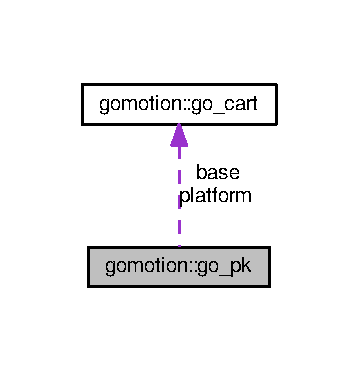
\includegraphics[width=172pt]{d2/d22/structgomotion_1_1go__pk__coll__graph}
\end{center}
\end{figure}
\subsection*{Data Fields}
\begin{DoxyCompactItemize}
\item 
\hyperlink{structgomotion_1_1go__cart}{go\-\_\-cart} \hyperlink{structgomotion_1_1go__pk_aaf6f59205aa710b5c9f04a49d13c6ac6}{base}
\item 
\hyperlink{structgomotion_1_1go__cart}{go\-\_\-cart} \hyperlink{structgomotion_1_1go__pk_ab3407e97c5c78c53e361609b52b78962}{platform}
\item 
\hyperlink{gotypes_8h_afd666a2393eebd71ee455846ac9def9b}{go\-\_\-real} \hyperlink{structgomotion_1_1go__pk_aca6d69ffde00a2f9b3f61af53c5e3377}{d}
\end{DoxyCompactItemize}


\subsection{Detailed Description}
P\-K parameters are used for parallel kinematic mechanisms, and represent the Cartesian positions of the ends of the link in the stationary base frame and the moving platform frame. Currently this only supports prismatic links. 

\subsection{Field Documentation}
\hypertarget{structgomotion_1_1go__pk_aaf6f59205aa710b5c9f04a49d13c6ac6}{\index{gomotion\-::go\-\_\-pk@{gomotion\-::go\-\_\-pk}!base@{base}}
\index{base@{base}!gomotion::go_pk@{gomotion\-::go\-\_\-pk}}
\subsubsection[{base}]{\setlength{\rightskip}{0pt plus 5cm}{\bf go\-\_\-cart} gomotion\-::go\-\_\-pk\-::base}}\label{structgomotion_1_1go__pk_aaf6f59205aa710b5c9f04a49d13c6ac6}
position of fixed end in base frame \hypertarget{structgomotion_1_1go__pk_aca6d69ffde00a2f9b3f61af53c5e3377}{\index{gomotion\-::go\-\_\-pk@{gomotion\-::go\-\_\-pk}!d@{d}}
\index{d@{d}!gomotion::go_pk@{gomotion\-::go\-\_\-pk}}
\subsubsection[{d}]{\setlength{\rightskip}{0pt plus 5cm}{\bf go\-\_\-real} gomotion\-::go\-\_\-pk\-::d}}\label{structgomotion_1_1go__pk_aca6d69ffde00a2f9b3f61af53c5e3377}
the length of the link \hypertarget{structgomotion_1_1go__pk_ab3407e97c5c78c53e361609b52b78962}{\index{gomotion\-::go\-\_\-pk@{gomotion\-::go\-\_\-pk}!platform@{platform}}
\index{platform@{platform}!gomotion::go_pk@{gomotion\-::go\-\_\-pk}}
\subsubsection[{platform}]{\setlength{\rightskip}{0pt plus 5cm}{\bf go\-\_\-cart} gomotion\-::go\-\_\-pk\-::platform}}\label{structgomotion_1_1go__pk_ab3407e97c5c78c53e361609b52b78962}
position of moving end in platform frame 

The documentation for this struct was generated from the following file\-:\begin{DoxyCompactItemize}
\item 
/usr/local/michalos/nistfanuc\-\_\-ws/src/gomotion/include/gomotion/\hyperlink{gomath_8h}{gomath.\-h}\end{DoxyCompactItemize}

\hypertarget{structgomotion_1_1go__plane}{\section{gomotion\-:\-:go\-\_\-plane Struct Reference}
\label{structgomotion_1_1go__plane}\index{gomotion\-::go\-\_\-plane@{gomotion\-::go\-\_\-plane}}
}


{\ttfamily \#include $<$gomath.\-h$>$}



Collaboration diagram for gomotion\-:\-:go\-\_\-plane\-:\nopagebreak
\begin{figure}[H]
\begin{center}
\leavevmode
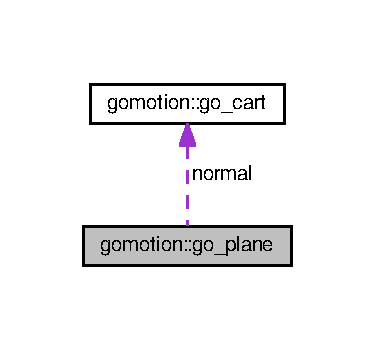
\includegraphics[width=180pt]{df/d22/structgomotion_1_1go__plane__coll__graph}
\end{center}
\end{figure}
\subsection*{Data Fields}
\begin{DoxyCompactItemize}
\item 
\hyperlink{structgomotion_1_1go__cart}{go\-\_\-cart} \hyperlink{structgomotion_1_1go__plane_a94d5e5a023dc4f396e2a60b9d396c427}{normal}
\item 
\hyperlink{gotypes_8h_afd666a2393eebd71ee455846ac9def9b}{go\-\_\-real} \hyperlink{structgomotion_1_1go__plane_a6397e783bfdfab04419cf41b809bc9e7}{d}
\end{DoxyCompactItemize}


\subsection{Detailed Description}
Given a plane as Ax + By + Cz + D = 0, the normal vector {\itshape normal} is the Cartesian vector (A,B,C), and the number {\itshape d} is the value D.

Planes have a handedness, given by the direction of the normal vector, so two planes that appear coincident may be different by the direction of their anti-\/parallel normal vectors. 

\subsection{Field Documentation}
\hypertarget{structgomotion_1_1go__plane_a6397e783bfdfab04419cf41b809bc9e7}{\index{gomotion\-::go\-\_\-plane@{gomotion\-::go\-\_\-plane}!d@{d}}
\index{d@{d}!gomotion::go_plane@{gomotion\-::go\-\_\-plane}}
\subsubsection[{d}]{\setlength{\rightskip}{0pt plus 5cm}{\bf go\-\_\-real} gomotion\-::go\-\_\-plane\-::d}}\label{structgomotion_1_1go__plane_a6397e783bfdfab04419cf41b809bc9e7}
\hypertarget{structgomotion_1_1go__plane_a94d5e5a023dc4f396e2a60b9d396c427}{\index{gomotion\-::go\-\_\-plane@{gomotion\-::go\-\_\-plane}!normal@{normal}}
\index{normal@{normal}!gomotion::go_plane@{gomotion\-::go\-\_\-plane}}
\subsubsection[{normal}]{\setlength{\rightskip}{0pt plus 5cm}{\bf go\-\_\-cart} gomotion\-::go\-\_\-plane\-::normal}}\label{structgomotion_1_1go__plane_a94d5e5a023dc4f396e2a60b9d396c427}


The documentation for this struct was generated from the following file\-:\begin{DoxyCompactItemize}
\item 
/usr/local/michalos/nistfanuc\-\_\-ws/src/gomotion/include/gomotion/\hyperlink{gomath_8h}{gomath.\-h}\end{DoxyCompactItemize}

\hypertarget{structgomotion_1_1go__pose}{\section{gomotion\-:\-:go\-\_\-pose Struct Reference}
\label{structgomotion_1_1go__pose}\index{gomotion\-::go\-\_\-pose@{gomotion\-::go\-\_\-pose}}
}


{\ttfamily \#include $<$gomath.\-h$>$}



Collaboration diagram for gomotion\-:\-:go\-\_\-pose\-:\nopagebreak
\begin{figure}[H]
\begin{center}
\leavevmode
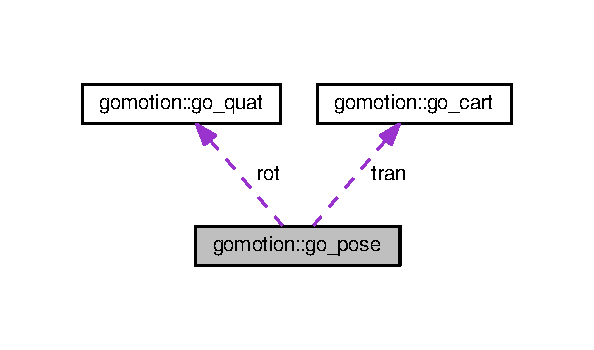
\includegraphics[width=285pt]{de/d41/structgomotion_1_1go__pose__coll__graph}
\end{center}
\end{figure}
\subsection*{Data Fields}
\begin{DoxyCompactItemize}
\item 
\hyperlink{structgomotion_1_1go__cart}{go\-\_\-cart} \hyperlink{structgomotion_1_1go__pose_afbe37cf24135dfc3cadf3536e88d7e8e}{tran}
\item 
\hyperlink{structgomotion_1_1go__quat}{go\-\_\-quat} \hyperlink{structgomotion_1_1go__pose_af30134c2f4d702ec890ec6726051cf8e}{rot}
\end{DoxyCompactItemize}


\subsection{Detailed Description}
A {\itshape \hyperlink{structgomotion_1_1go__pose}{go\-\_\-pose}} represents the Cartesian position vector and quaternion orientation of a frame. 

\subsection{Field Documentation}
\hypertarget{structgomotion_1_1go__pose_af30134c2f4d702ec890ec6726051cf8e}{\index{gomotion\-::go\-\_\-pose@{gomotion\-::go\-\_\-pose}!rot@{rot}}
\index{rot@{rot}!gomotion::go_pose@{gomotion\-::go\-\_\-pose}}
\subsubsection[{rot}]{\setlength{\rightskip}{0pt plus 5cm}{\bf go\-\_\-quat} gomotion\-::go\-\_\-pose\-::rot}}\label{structgomotion_1_1go__pose_af30134c2f4d702ec890ec6726051cf8e}
\hypertarget{structgomotion_1_1go__pose_afbe37cf24135dfc3cadf3536e88d7e8e}{\index{gomotion\-::go\-\_\-pose@{gomotion\-::go\-\_\-pose}!tran@{tran}}
\index{tran@{tran}!gomotion::go_pose@{gomotion\-::go\-\_\-pose}}
\subsubsection[{tran}]{\setlength{\rightskip}{0pt plus 5cm}{\bf go\-\_\-cart} gomotion\-::go\-\_\-pose\-::tran}}\label{structgomotion_1_1go__pose_afbe37cf24135dfc3cadf3536e88d7e8e}


The documentation for this struct was generated from the following file\-:\begin{DoxyCompactItemize}
\item 
/usr/local/michalos/nistfanuc\-\_\-ws/src/gomotion/include/gomotion/\hyperlink{gomath_8h}{gomath.\-h}\end{DoxyCompactItemize}

\hypertarget{structgomotion_1_1go__position}{\section{gomotion\-:\-:go\-\_\-position Struct Reference}
\label{structgomotion_1_1go__position}\index{gomotion\-::go\-\_\-position@{gomotion\-::go\-\_\-position}}
}


Container for a joint position or Cartesian position. Depending upon whether you are doing joint interpolation or world coordinate interpolation (as specified by your call to go\-\_\-motion\-\_\-queue\-\_\-set\-\_\-type()), fill in joint\mbox{[}\mbox{]} or pose accordingly.  




{\ttfamily \#include $<$gomotion.\-h$>$}

\subsection*{Public Member Functions}
\begin{DoxyCompactItemize}
\item 
\hypertarget{structgomotion_1_1go__position_af075d5442765600dd50494b47161db4b}{void {\bfseries zero\-\_\-joints} ()}\label{structgomotion_1_1go__position_af075d5442765600dd50494b47161db4b}

\item 
\hypertarget{structgomotion_1_1go__position_ab319ce59146e5f8313bdb5d1b7001617}{void {\bfseries zero\-\_\-pose} ()}\label{structgomotion_1_1go__position_ab319ce59146e5f8313bdb5d1b7001617}

\end{DoxyCompactItemize}
\subsection*{Public Attributes}
\begin{DoxyCompactItemize}
\item 
\hypertarget{structgomotion_1_1go__position_a54de5215a676f5e6bc004ec15803a2cb}{\begin{tabbing}
xx\=xx\=xx\=xx\=xx\=xx\=xx\=xx\=xx\=\kill
union \{\\
\hypertarget{uniongomotion_1_1go__position_1_1@1_abe054c50898120fd6b1b260edf8f0074}{\>go\_real {\bfseries joint} \mbox{[}GO\_MOTION\_JOINT\_NUM\mbox{]}\\
\hypertarget{uniongomotion_1_1go__position_1_1@1_a52e09e22901615c1ca71757ea57215ca}{\>go\_pose {\bfseries pose}\\
\} {\bfseries u}}\label{structgomotion_1_1go__position_a54de5215a676f5e6bc004ec15803a2cb}
\\

\end{tabbing}\end{DoxyCompactItemize}


\subsection{Detailed Description}
Container for a joint position or Cartesian position. Depending upon whether you are doing joint interpolation or world coordinate interpolation (as specified by your call to go\-\_\-motion\-\_\-queue\-\_\-set\-\_\-type()), fill in joint\mbox{[}\mbox{]} or pose accordingly. 

The documentation for this struct was generated from the following file\-:\begin{DoxyCompactItemize}
\item 
/usr/local/michalos/nistfanuc\-\_\-ws/src/gomotion/include/gomotion/\hyperlink{gomotion_8h}{gomotion.\-h}\end{DoxyCompactItemize}

\hypertarget{structgomotion_1_1go__pp}{\section{gomotion\-:\-:go\-\_\-pp Struct Reference}
\label{structgomotion_1_1go__pp}\index{gomotion\-::go\-\_\-pp@{gomotion\-::go\-\_\-pp}}
}


{\ttfamily \#include $<$gomath.\-h$>$}



Collaboration diagram for gomotion\-:\-:go\-\_\-pp\-:\nopagebreak
\begin{figure}[H]
\begin{center}
\leavevmode
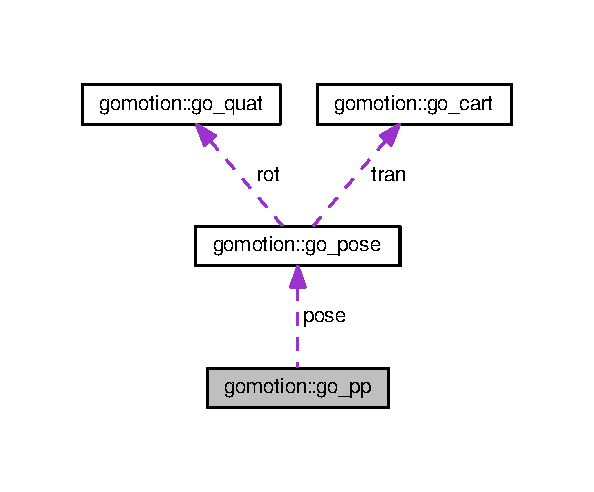
\includegraphics[width=285pt]{db/d6b/structgomotion_1_1go__pp__coll__graph}
\end{center}
\end{figure}
\subsection*{Data Fields}
\begin{DoxyCompactItemize}
\item 
\hyperlink{structgomotion_1_1go__pose}{go\-\_\-pose} \hyperlink{structgomotion_1_1go__pp_a93d5d228709c062d8bcd465276e9f399}{pose}
\end{DoxyCompactItemize}


\subsection{Detailed Description}
P\-P parameters represent the pose of the link with respect to the previous link. Revolute joints rotate about the Z axis, prismatic joints slide along the Z axis. 

\subsection{Field Documentation}
\hypertarget{structgomotion_1_1go__pp_a93d5d228709c062d8bcd465276e9f399}{\index{gomotion\-::go\-\_\-pp@{gomotion\-::go\-\_\-pp}!pose@{pose}}
\index{pose@{pose}!gomotion::go_pp@{gomotion\-::go\-\_\-pp}}
\subsubsection[{pose}]{\setlength{\rightskip}{0pt plus 5cm}{\bf go\-\_\-pose} gomotion\-::go\-\_\-pp\-::pose}}\label{structgomotion_1_1go__pp_a93d5d228709c062d8bcd465276e9f399}
the pose of the link wrt to the previous link 

The documentation for this struct was generated from the following file\-:\begin{DoxyCompactItemize}
\item 
/usr/local/michalos/nistfanuc\-\_\-ws/src/gomotion/include/gomotion/\hyperlink{gomath_8h}{gomath.\-h}\end{DoxyCompactItemize}

\hypertarget{structgomotion_1_1go__quadratic}{\section{gomotion\-:\-:go\-\_\-quadratic Struct Reference}
\label{structgomotion_1_1go__quadratic}\index{gomotion\-::go\-\_\-quadratic@{gomotion\-::go\-\_\-quadratic}}
}


{\ttfamily \#include $<$gomath.\-h$>$}

\subsection*{Data Fields}
\begin{DoxyCompactItemize}
\item 
\hyperlink{gotypes_8h_afd666a2393eebd71ee455846ac9def9b}{go\-\_\-real} \hyperlink{structgomotion_1_1go__quadratic_a6c7ae9e2f77e687015fc736848971e5c}{a}
\item 
\hyperlink{gotypes_8h_afd666a2393eebd71ee455846ac9def9b}{go\-\_\-real} \hyperlink{structgomotion_1_1go__quadratic_ae06e4da9f9ffdf7a19149dcf40b92073}{b}
\end{DoxyCompactItemize}


\subsection{Field Documentation}
\hypertarget{structgomotion_1_1go__quadratic_a6c7ae9e2f77e687015fc736848971e5c}{\index{gomotion\-::go\-\_\-quadratic@{gomotion\-::go\-\_\-quadratic}!a@{a}}
\index{a@{a}!gomotion::go_quadratic@{gomotion\-::go\-\_\-quadratic}}
\subsubsection[{a}]{\setlength{\rightskip}{0pt plus 5cm}{\bf go\-\_\-real} gomotion\-::go\-\_\-quadratic\-::a}}\label{structgomotion_1_1go__quadratic_a6c7ae9e2f77e687015fc736848971e5c}
\hypertarget{structgomotion_1_1go__quadratic_ae06e4da9f9ffdf7a19149dcf40b92073}{\index{gomotion\-::go\-\_\-quadratic@{gomotion\-::go\-\_\-quadratic}!b@{b}}
\index{b@{b}!gomotion::go_quadratic@{gomotion\-::go\-\_\-quadratic}}
\subsubsection[{b}]{\setlength{\rightskip}{0pt plus 5cm}{\bf go\-\_\-real} gomotion\-::go\-\_\-quadratic\-::b}}\label{structgomotion_1_1go__quadratic_ae06e4da9f9ffdf7a19149dcf40b92073}


The documentation for this struct was generated from the following file\-:\begin{DoxyCompactItemize}
\item 
/usr/local/michalos/nistfanuc\-\_\-ws/src/gomotion/include/gomotion/\hyperlink{gomath_8h}{gomath.\-h}\end{DoxyCompactItemize}

\hypertarget{structgomotion_1_1go__quartic}{\section{gomotion\-:\-:go\-\_\-quartic Struct Reference}
\label{structgomotion_1_1go__quartic}\index{gomotion\-::go\-\_\-quartic@{gomotion\-::go\-\_\-quartic}}
}


{\ttfamily \#include $<$gomath.\-h$>$}

\subsection*{Data Fields}
\begin{DoxyCompactItemize}
\item 
\hyperlink{gotypes_8h_afd666a2393eebd71ee455846ac9def9b}{go\-\_\-real} \hyperlink{structgomotion_1_1go__quartic_a160b6aab2661877f8027d8eaf0db0d32}{a}
\item 
\hyperlink{gotypes_8h_afd666a2393eebd71ee455846ac9def9b}{go\-\_\-real} \hyperlink{structgomotion_1_1go__quartic_a7fc463501a38f59900914bc8f93c5c84}{b}
\item 
\hyperlink{gotypes_8h_afd666a2393eebd71ee455846ac9def9b}{go\-\_\-real} \hyperlink{structgomotion_1_1go__quartic_a0b6d02bd495ab899be138928394c4d46}{c}
\item 
\hyperlink{gotypes_8h_afd666a2393eebd71ee455846ac9def9b}{go\-\_\-real} \hyperlink{structgomotion_1_1go__quartic_a27261754dea678a29b22ecc87fe2f3f5}{d}
\end{DoxyCompactItemize}


\subsection{Field Documentation}
\hypertarget{structgomotion_1_1go__quartic_a160b6aab2661877f8027d8eaf0db0d32}{\index{gomotion\-::go\-\_\-quartic@{gomotion\-::go\-\_\-quartic}!a@{a}}
\index{a@{a}!gomotion::go_quartic@{gomotion\-::go\-\_\-quartic}}
\subsubsection[{a}]{\setlength{\rightskip}{0pt plus 5cm}{\bf go\-\_\-real} gomotion\-::go\-\_\-quartic\-::a}}\label{structgomotion_1_1go__quartic_a160b6aab2661877f8027d8eaf0db0d32}
\hypertarget{structgomotion_1_1go__quartic_a7fc463501a38f59900914bc8f93c5c84}{\index{gomotion\-::go\-\_\-quartic@{gomotion\-::go\-\_\-quartic}!b@{b}}
\index{b@{b}!gomotion::go_quartic@{gomotion\-::go\-\_\-quartic}}
\subsubsection[{b}]{\setlength{\rightskip}{0pt plus 5cm}{\bf go\-\_\-real} gomotion\-::go\-\_\-quartic\-::b}}\label{structgomotion_1_1go__quartic_a7fc463501a38f59900914bc8f93c5c84}
\hypertarget{structgomotion_1_1go__quartic_a0b6d02bd495ab899be138928394c4d46}{\index{gomotion\-::go\-\_\-quartic@{gomotion\-::go\-\_\-quartic}!c@{c}}
\index{c@{c}!gomotion::go_quartic@{gomotion\-::go\-\_\-quartic}}
\subsubsection[{c}]{\setlength{\rightskip}{0pt plus 5cm}{\bf go\-\_\-real} gomotion\-::go\-\_\-quartic\-::c}}\label{structgomotion_1_1go__quartic_a0b6d02bd495ab899be138928394c4d46}
\hypertarget{structgomotion_1_1go__quartic_a27261754dea678a29b22ecc87fe2f3f5}{\index{gomotion\-::go\-\_\-quartic@{gomotion\-::go\-\_\-quartic}!d@{d}}
\index{d@{d}!gomotion::go_quartic@{gomotion\-::go\-\_\-quartic}}
\subsubsection[{d}]{\setlength{\rightskip}{0pt plus 5cm}{\bf go\-\_\-real} gomotion\-::go\-\_\-quartic\-::d}}\label{structgomotion_1_1go__quartic_a27261754dea678a29b22ecc87fe2f3f5}


The documentation for this struct was generated from the following file\-:\begin{DoxyCompactItemize}
\item 
/usr/local/michalos/nistfanuc\-\_\-ws/src/gomotion/include/gomotion/\hyperlink{gomath_8h}{gomath.\-h}\end{DoxyCompactItemize}

\hypertarget{structgomotion_1_1go__quat}{\section{gomotion\-:\-:go\-\_\-quat Struct Reference}
\label{structgomotion_1_1go__quat}\index{gomotion\-::go\-\_\-quat@{gomotion\-::go\-\_\-quat}}
}


{\ttfamily \#include $<$gomath.\-h$>$}

\subsection*{Data Fields}
\begin{DoxyCompactItemize}
\item 
\hyperlink{gotypes_8h_afd666a2393eebd71ee455846ac9def9b}{go\-\_\-real} \hyperlink{structgomotion_1_1go__quat_aad82d91646627a2c9ca3256d4bede64a}{s}
\item 
\hyperlink{gotypes_8h_afd666a2393eebd71ee455846ac9def9b}{go\-\_\-real} \hyperlink{structgomotion_1_1go__quat_a009660cf4962202e569fbe41b490722f}{x}
\item 
\hyperlink{gotypes_8h_afd666a2393eebd71ee455846ac9def9b}{go\-\_\-real} \hyperlink{structgomotion_1_1go__quat_a837f1ac99a7c09b80414f232e16ed1de}{y}
\item 
\hyperlink{gotypes_8h_afd666a2393eebd71ee455846ac9def9b}{go\-\_\-real} \hyperlink{structgomotion_1_1go__quat_a1ef5cc0b14458e74b4f47d4ccbc90f39}{z}
\end{DoxyCompactItemize}


\subsection{Detailed Description}
A quaternion. {\itshape s} is the cosine of the half angle of rotation, and the {\itshape xyz} elements comprise the vector that points in the direction of positive rotation and whose magnitude is the sine of the half angle of rotation. 

\subsection{Field Documentation}
\hypertarget{structgomotion_1_1go__quat_aad82d91646627a2c9ca3256d4bede64a}{\index{gomotion\-::go\-\_\-quat@{gomotion\-::go\-\_\-quat}!s@{s}}
\index{s@{s}!gomotion::go_quat@{gomotion\-::go\-\_\-quat}}
\subsubsection[{s}]{\setlength{\rightskip}{0pt plus 5cm}{\bf go\-\_\-real} gomotion\-::go\-\_\-quat\-::s}}\label{structgomotion_1_1go__quat_aad82d91646627a2c9ca3256d4bede64a}
\hypertarget{structgomotion_1_1go__quat_a009660cf4962202e569fbe41b490722f}{\index{gomotion\-::go\-\_\-quat@{gomotion\-::go\-\_\-quat}!x@{x}}
\index{x@{x}!gomotion::go_quat@{gomotion\-::go\-\_\-quat}}
\subsubsection[{x}]{\setlength{\rightskip}{0pt plus 5cm}{\bf go\-\_\-real} gomotion\-::go\-\_\-quat\-::x}}\label{structgomotion_1_1go__quat_a009660cf4962202e569fbe41b490722f}
\hypertarget{structgomotion_1_1go__quat_a837f1ac99a7c09b80414f232e16ed1de}{\index{gomotion\-::go\-\_\-quat@{gomotion\-::go\-\_\-quat}!y@{y}}
\index{y@{y}!gomotion::go_quat@{gomotion\-::go\-\_\-quat}}
\subsubsection[{y}]{\setlength{\rightskip}{0pt plus 5cm}{\bf go\-\_\-real} gomotion\-::go\-\_\-quat\-::y}}\label{structgomotion_1_1go__quat_a837f1ac99a7c09b80414f232e16ed1de}
\hypertarget{structgomotion_1_1go__quat_a1ef5cc0b14458e74b4f47d4ccbc90f39}{\index{gomotion\-::go\-\_\-quat@{gomotion\-::go\-\_\-quat}!z@{z}}
\index{z@{z}!gomotion::go_quat@{gomotion\-::go\-\_\-quat}}
\subsubsection[{z}]{\setlength{\rightskip}{0pt plus 5cm}{\bf go\-\_\-real} gomotion\-::go\-\_\-quat\-::z}}\label{structgomotion_1_1go__quat_a1ef5cc0b14458e74b4f47d4ccbc90f39}


The documentation for this struct was generated from the following file\-:\begin{DoxyCompactItemize}
\item 
/usr/local/michalos/nistfanuc\-\_\-ws/src/gomotion/include/gomotion/\hyperlink{gomath_8h}{gomath.\-h}\end{DoxyCompactItemize}

\hypertarget{structgomotion_1_1go__rpy}{\section{gomotion\-:\-:go\-\_\-rpy Struct Reference}
\label{structgomotion_1_1go__rpy}\index{gomotion\-::go\-\_\-rpy@{gomotion\-::go\-\_\-rpy}}
}


{\ttfamily \#include $<$gomath.\-h$>$}

\subsection*{Data Fields}
\begin{DoxyCompactItemize}
\item 
\hyperlink{gotypes_8h_afd666a2393eebd71ee455846ac9def9b}{go\-\_\-real} \hyperlink{structgomotion_1_1go__rpy_a37241d3fe9431d408add42f27e395154}{r}
\item 
\hyperlink{gotypes_8h_afd666a2393eebd71ee455846ac9def9b}{go\-\_\-real} \hyperlink{structgomotion_1_1go__rpy_a309f825360e8b7b41577208d606f3e4d}{p}
\item 
\hyperlink{gotypes_8h_afd666a2393eebd71ee455846ac9def9b}{go\-\_\-real} \hyperlink{structgomotion_1_1go__rpy_a38a63e8c2a10283b56c3a697f142f8e2}{y}
\end{DoxyCompactItemize}


\subsection{Detailed Description}
Roll-\/pitch-\/yaw angles. {\itshape r} is the amount of the first rotation (roll) around the X axis. {\itshape p} is the amount of the second rotation (pitch) around the original Y axis. {\itshape y} is the amount of the third rotation (yaw) around the original Z axis. 

\subsection{Field Documentation}
\hypertarget{structgomotion_1_1go__rpy_a309f825360e8b7b41577208d606f3e4d}{\index{gomotion\-::go\-\_\-rpy@{gomotion\-::go\-\_\-rpy}!p@{p}}
\index{p@{p}!gomotion::go_rpy@{gomotion\-::go\-\_\-rpy}}
\subsubsection[{p}]{\setlength{\rightskip}{0pt plus 5cm}{\bf go\-\_\-real} gomotion\-::go\-\_\-rpy\-::p}}\label{structgomotion_1_1go__rpy_a309f825360e8b7b41577208d606f3e4d}
\hypertarget{structgomotion_1_1go__rpy_a37241d3fe9431d408add42f27e395154}{\index{gomotion\-::go\-\_\-rpy@{gomotion\-::go\-\_\-rpy}!r@{r}}
\index{r@{r}!gomotion::go_rpy@{gomotion\-::go\-\_\-rpy}}
\subsubsection[{r}]{\setlength{\rightskip}{0pt plus 5cm}{\bf go\-\_\-real} gomotion\-::go\-\_\-rpy\-::r}}\label{structgomotion_1_1go__rpy_a37241d3fe9431d408add42f27e395154}
\hypertarget{structgomotion_1_1go__rpy_a38a63e8c2a10283b56c3a697f142f8e2}{\index{gomotion\-::go\-\_\-rpy@{gomotion\-::go\-\_\-rpy}!y@{y}}
\index{y@{y}!gomotion::go_rpy@{gomotion\-::go\-\_\-rpy}}
\subsubsection[{y}]{\setlength{\rightskip}{0pt plus 5cm}{\bf go\-\_\-real} gomotion\-::go\-\_\-rpy\-::y}}\label{structgomotion_1_1go__rpy_a38a63e8c2a10283b56c3a697f142f8e2}


The documentation for this struct was generated from the following file\-:\begin{DoxyCompactItemize}
\item 
/usr/local/michalos/nistfanuc\-\_\-ws/src/gomotion/include/gomotion/\hyperlink{gomath_8h}{gomath.\-h}\end{DoxyCompactItemize}

\hypertarget{structgomotion_1_1go__rvec}{\section{gomotion\-:\-:go\-\_\-rvec Struct Reference}
\label{structgomotion_1_1go__rvec}\index{gomotion\-::go\-\_\-rvec@{gomotion\-::go\-\_\-rvec}}
}


{\ttfamily \#include $<$gomath.\-h$>$}

\subsection*{Data Fields}
\begin{DoxyCompactItemize}
\item 
\hyperlink{gotypes_8h_afd666a2393eebd71ee455846ac9def9b}{go\-\_\-real} \hyperlink{structgomotion_1_1go__rvec_ae29a06bf1a12fc0d321442026f513117}{x}
\item 
\hyperlink{gotypes_8h_afd666a2393eebd71ee455846ac9def9b}{go\-\_\-real} \hyperlink{structgomotion_1_1go__rvec_a5f560402a28bd1cf2ced1cdd627e8e30}{y}
\item 
\hyperlink{gotypes_8h_afd666a2393eebd71ee455846ac9def9b}{go\-\_\-real} \hyperlink{structgomotion_1_1go__rvec_a47712173e216ec298c4d58af0abfb100}{z}
\end{DoxyCompactItemize}


\subsection{Detailed Description}
A rotation vector, whose direction points along the axis of positive rotation, and whose magnitude is the amount of rotation around this axis, in radians. 

\subsection{Field Documentation}
\hypertarget{structgomotion_1_1go__rvec_ae29a06bf1a12fc0d321442026f513117}{\index{gomotion\-::go\-\_\-rvec@{gomotion\-::go\-\_\-rvec}!x@{x}}
\index{x@{x}!gomotion::go_rvec@{gomotion\-::go\-\_\-rvec}}
\subsubsection[{x}]{\setlength{\rightskip}{0pt plus 5cm}{\bf go\-\_\-real} gomotion\-::go\-\_\-rvec\-::x}}\label{structgomotion_1_1go__rvec_ae29a06bf1a12fc0d321442026f513117}
\hypertarget{structgomotion_1_1go__rvec_a5f560402a28bd1cf2ced1cdd627e8e30}{\index{gomotion\-::go\-\_\-rvec@{gomotion\-::go\-\_\-rvec}!y@{y}}
\index{y@{y}!gomotion::go_rvec@{gomotion\-::go\-\_\-rvec}}
\subsubsection[{y}]{\setlength{\rightskip}{0pt plus 5cm}{\bf go\-\_\-real} gomotion\-::go\-\_\-rvec\-::y}}\label{structgomotion_1_1go__rvec_a5f560402a28bd1cf2ced1cdd627e8e30}
\hypertarget{structgomotion_1_1go__rvec_a47712173e216ec298c4d58af0abfb100}{\index{gomotion\-::go\-\_\-rvec@{gomotion\-::go\-\_\-rvec}!z@{z}}
\index{z@{z}!gomotion::go_rvec@{gomotion\-::go\-\_\-rvec}}
\subsubsection[{z}]{\setlength{\rightskip}{0pt plus 5cm}{\bf go\-\_\-real} gomotion\-::go\-\_\-rvec\-::z}}\label{structgomotion_1_1go__rvec_a47712173e216ec298c4d58af0abfb100}


The documentation for this struct was generated from the following file\-:\begin{DoxyCompactItemize}
\item 
/usr/local/michalos/nistfanuc\-\_\-ws/src/gomotion/include/gomotion/\hyperlink{gomath_8h}{gomath.\-h}\end{DoxyCompactItemize}

\hypertarget{structgomotion_1_1go__scale__spec}{\section{gomotion\-:\-:go\-\_\-scale\-\_\-spec Struct Reference}
\label{structgomotion_1_1go__scale__spec}\index{gomotion\-::go\-\_\-scale\-\_\-spec@{gomotion\-::go\-\_\-scale\-\_\-spec}}
}
\subsection*{Public Member Functions}
\begin{DoxyCompactItemize}
\item 
\hypertarget{structgomotion_1_1go__scale__spec_ab10fecb573317c67528eb4d370705129}{go\-\_\-result {\bfseries init} (go\-\_\-real \hyperlink{structgomotion_1_1go__scale__spec_a592f5bd1c5d775d30e25b798900a2c30}{scale})}\label{structgomotion_1_1go__scale__spec_ab10fecb573317c67528eb4d370705129}

\item 
\hypertarget{structgomotion_1_1go__scale__spec_af98067c5057e4a27be45c932d40b1ee3}{go\-\_\-result {\bfseries set} (go\-\_\-real \hyperlink{structgomotion_1_1go__scale__spec_a592f5bd1c5d775d30e25b798900a2c30}{scale}, go\-\_\-real scale\-\_\-v, go\-\_\-real scale\-\_\-a)}\label{structgomotion_1_1go__scale__spec_af98067c5057e4a27be45c932d40b1ee3}

\item 
\hypertarget{structgomotion_1_1go__scale__spec_a8eaf5f40d5b5ee430ae70a1f4fbcff1e}{go\-\_\-result {\bfseries eval} (go\-\_\-real deltat, go\-\_\-real $\ast$\hyperlink{structgomotion_1_1go__scale__spec_a592f5bd1c5d775d30e25b798900a2c30}{scale})}\label{structgomotion_1_1go__scale__spec_a8eaf5f40d5b5ee430ae70a1f4fbcff1e}

\end{DoxyCompactItemize}
\subsection*{Public Attributes}
\begin{DoxyCompactItemize}
\item 
\hypertarget{structgomotion_1_1go__scale__spec_a09627b5c232ccc27aa4a9876c7fd6edb}{go\-\_\-traj\-\_\-ca\-\_\-spec {\bfseries scale\-\_\-spec}}\label{structgomotion_1_1go__scale__spec_a09627b5c232ccc27aa4a9876c7fd6edb}

\item 
go\-\_\-flag \hyperlink{structgomotion_1_1go__scale__spec_ab692a7752aa08649020c990b4bea3c84}{scaling}
\item 
go\-\_\-flag \hyperlink{structgomotion_1_1go__scale__spec_af13cc2a23a17aba5aae5fbafc47a8428}{scale\-\_\-dir}
\item 
go\-\_\-flag \hyperlink{structgomotion_1_1go__scale__spec_abd719098dc45e827d7349e8eb682f2c2}{scale\-\_\-isneg}
\item 
go\-\_\-real \hyperlink{structgomotion_1_1go__scale__spec_ac734b7e45bc1da45992fdf6f1fdc792d}{scale\-\_\-b}
\item 
go\-\_\-real \hyperlink{structgomotion_1_1go__scale__spec_a592f5bd1c5d775d30e25b798900a2c30}{scale}
\item 
go\-\_\-real \hyperlink{structgomotion_1_1go__scale__spec_ab141b03f6bb455d94cbeebf6c9de5cc3}{scale\-\_\-next}
\item 
go\-\_\-real \hyperlink{structgomotion_1_1go__scale__spec_a72b34038e403e2efffd083765389c5f2}{scale\-\_\-v\-\_\-next}
\item 
go\-\_\-real \hyperlink{structgomotion_1_1go__scale__spec_a1786056a5451cb1841cf42f23f079c61}{scale\-\_\-a\-\_\-next}
\item 
go\-\_\-real \hyperlink{structgomotion_1_1go__scale__spec_a7496e98c2084abd59d74c803b1d7dbec}{scale\-\_\-t}
\end{DoxyCompactItemize}


\subsection{Member Data Documentation}
\hypertarget{structgomotion_1_1go__scale__spec_a592f5bd1c5d775d30e25b798900a2c30}{\index{gomotion\-::go\-\_\-scale\-\_\-spec@{gomotion\-::go\-\_\-scale\-\_\-spec}!scale@{scale}}
\index{scale@{scale}!gomotion::go_scale_spec@{gomotion\-::go\-\_\-scale\-\_\-spec}}
\subsubsection[{scale}]{\setlength{\rightskip}{0pt plus 5cm}go\-\_\-real gomotion\-::go\-\_\-scale\-\_\-spec\-::scale}}\label{structgomotion_1_1go__scale__spec_a592f5bd1c5d775d30e25b798900a2c30}
current scale factor \hypertarget{structgomotion_1_1go__scale__spec_a1786056a5451cb1841cf42f23f079c61}{\index{gomotion\-::go\-\_\-scale\-\_\-spec@{gomotion\-::go\-\_\-scale\-\_\-spec}!scale\-\_\-a\-\_\-next@{scale\-\_\-a\-\_\-next}}
\index{scale\-\_\-a\-\_\-next@{scale\-\_\-a\-\_\-next}!gomotion::go_scale_spec@{gomotion\-::go\-\_\-scale\-\_\-spec}}
\subsubsection[{scale\-\_\-a\-\_\-next}]{\setlength{\rightskip}{0pt plus 5cm}go\-\_\-real gomotion\-::go\-\_\-scale\-\_\-spec\-::scale\-\_\-a\-\_\-next}}\label{structgomotion_1_1go__scale__spec_a1786056a5451cb1841cf42f23f079c61}
pending d$^\wedge$2(scale)/dt$^\wedge$2 \hypertarget{structgomotion_1_1go__scale__spec_ac734b7e45bc1da45992fdf6f1fdc792d}{\index{gomotion\-::go\-\_\-scale\-\_\-spec@{gomotion\-::go\-\_\-scale\-\_\-spec}!scale\-\_\-b@{scale\-\_\-b}}
\index{scale\-\_\-b@{scale\-\_\-b}!gomotion::go_scale_spec@{gomotion\-::go\-\_\-scale\-\_\-spec}}
\subsubsection[{scale\-\_\-b}]{\setlength{\rightskip}{0pt plus 5cm}go\-\_\-real gomotion\-::go\-\_\-scale\-\_\-spec\-::scale\-\_\-b}}\label{structgomotion_1_1go__scale__spec_ac734b7e45bc1da45992fdf6f1fdc792d}
original base scale factor \hypertarget{structgomotion_1_1go__scale__spec_af13cc2a23a17aba5aae5fbafc47a8428}{\index{gomotion\-::go\-\_\-scale\-\_\-spec@{gomotion\-::go\-\_\-scale\-\_\-spec}!scale\-\_\-dir@{scale\-\_\-dir}}
\index{scale\-\_\-dir@{scale\-\_\-dir}!gomotion::go_scale_spec@{gomotion\-::go\-\_\-scale\-\_\-spec}}
\subsubsection[{scale\-\_\-dir}]{\setlength{\rightskip}{0pt plus 5cm}go\-\_\-flag gomotion\-::go\-\_\-scale\-\_\-spec\-::scale\-\_\-dir}}\label{structgomotion_1_1go__scale__spec_af13cc2a23a17aba5aae5fbafc47a8428}
non-\/zero means add scale to scale\-\_\-b \hypertarget{structgomotion_1_1go__scale__spec_abd719098dc45e827d7349e8eb682f2c2}{\index{gomotion\-::go\-\_\-scale\-\_\-spec@{gomotion\-::go\-\_\-scale\-\_\-spec}!scale\-\_\-isneg@{scale\-\_\-isneg}}
\index{scale\-\_\-isneg@{scale\-\_\-isneg}!gomotion::go_scale_spec@{gomotion\-::go\-\_\-scale\-\_\-spec}}
\subsubsection[{scale\-\_\-isneg}]{\setlength{\rightskip}{0pt plus 5cm}go\-\_\-flag gomotion\-::go\-\_\-scale\-\_\-spec\-::scale\-\_\-isneg}}\label{structgomotion_1_1go__scale__spec_abd719098dc45e827d7349e8eb682f2c2}
non-\/zero means negative scale \hypertarget{structgomotion_1_1go__scale__spec_ab141b03f6bb455d94cbeebf6c9de5cc3}{\index{gomotion\-::go\-\_\-scale\-\_\-spec@{gomotion\-::go\-\_\-scale\-\_\-spec}!scale\-\_\-next@{scale\-\_\-next}}
\index{scale\-\_\-next@{scale\-\_\-next}!gomotion::go_scale_spec@{gomotion\-::go\-\_\-scale\-\_\-spec}}
\subsubsection[{scale\-\_\-next}]{\setlength{\rightskip}{0pt plus 5cm}go\-\_\-real gomotion\-::go\-\_\-scale\-\_\-spec\-::scale\-\_\-next}}\label{structgomotion_1_1go__scale__spec_ab141b03f6bb455d94cbeebf6c9de5cc3}
pending scale factor \hypertarget{structgomotion_1_1go__scale__spec_a7496e98c2084abd59d74c803b1d7dbec}{\index{gomotion\-::go\-\_\-scale\-\_\-spec@{gomotion\-::go\-\_\-scale\-\_\-spec}!scale\-\_\-t@{scale\-\_\-t}}
\index{scale\-\_\-t@{scale\-\_\-t}!gomotion::go_scale_spec@{gomotion\-::go\-\_\-scale\-\_\-spec}}
\subsubsection[{scale\-\_\-t}]{\setlength{\rightskip}{0pt plus 5cm}go\-\_\-real gomotion\-::go\-\_\-scale\-\_\-spec\-::scale\-\_\-t}}\label{structgomotion_1_1go__scale__spec_a7496e98c2084abd59d74c803b1d7dbec}
time into scaling \hypertarget{structgomotion_1_1go__scale__spec_a72b34038e403e2efffd083765389c5f2}{\index{gomotion\-::go\-\_\-scale\-\_\-spec@{gomotion\-::go\-\_\-scale\-\_\-spec}!scale\-\_\-v\-\_\-next@{scale\-\_\-v\-\_\-next}}
\index{scale\-\_\-v\-\_\-next@{scale\-\_\-v\-\_\-next}!gomotion::go_scale_spec@{gomotion\-::go\-\_\-scale\-\_\-spec}}
\subsubsection[{scale\-\_\-v\-\_\-next}]{\setlength{\rightskip}{0pt plus 5cm}go\-\_\-real gomotion\-::go\-\_\-scale\-\_\-spec\-::scale\-\_\-v\-\_\-next}}\label{structgomotion_1_1go__scale__spec_a72b34038e403e2efffd083765389c5f2}
pending d(scale)/dt \hypertarget{structgomotion_1_1go__scale__spec_ab692a7752aa08649020c990b4bea3c84}{\index{gomotion\-::go\-\_\-scale\-\_\-spec@{gomotion\-::go\-\_\-scale\-\_\-spec}!scaling@{scaling}}
\index{scaling@{scaling}!gomotion::go_scale_spec@{gomotion\-::go\-\_\-scale\-\_\-spec}}
\subsubsection[{scaling}]{\setlength{\rightskip}{0pt plus 5cm}go\-\_\-flag gomotion\-::go\-\_\-scale\-\_\-spec\-::scaling}}\label{structgomotion_1_1go__scale__spec_ab692a7752aa08649020c990b4bea3c84}
non-\/zero means we're scaling time 

The documentation for this struct was generated from the following file\-:\begin{DoxyCompactItemize}
\item 
/usr/local/michalos/nistfanuc\-\_\-ws/src/gomotion/include/gomotion/\hyperlink{gomotion_8h}{gomotion.\-h}\end{DoxyCompactItemize}

\hypertarget{structgomotion_1_1go__sph}{\section{gomotion\-:\-:go\-\_\-sph Struct Reference}
\label{structgomotion_1_1go__sph}\index{gomotion\-::go\-\_\-sph@{gomotion\-::go\-\_\-sph}}
}


{\ttfamily \#include $<$gomath.\-h$>$}

\subsection*{Data Fields}
\begin{DoxyCompactItemize}
\item 
\hyperlink{gotypes_8h_afd666a2393eebd71ee455846ac9def9b}{go\-\_\-real} \hyperlink{structgomotion_1_1go__sph_ad922b1e1556ad041c62ae71e2335e688}{theta}
\item 
\hyperlink{gotypes_8h_afd666a2393eebd71ee455846ac9def9b}{go\-\_\-real} \hyperlink{structgomotion_1_1go__sph_afd0964fc26067714ed465d2ea36ea90d}{phi}
\item 
\hyperlink{gotypes_8h_afd666a2393eebd71ee455846ac9def9b}{go\-\_\-real} \hyperlink{structgomotion_1_1go__sph_a44361cc285fdc563622c7f74121bc5d8}{r}
\end{DoxyCompactItemize}


\subsection{Detailed Description}
A point or vector in spherical coordinates, with {\itshape phi} as the angle down from the zenith, not up from the X\-Y plane. 

\subsection{Field Documentation}
\hypertarget{structgomotion_1_1go__sph_afd0964fc26067714ed465d2ea36ea90d}{\index{gomotion\-::go\-\_\-sph@{gomotion\-::go\-\_\-sph}!phi@{phi}}
\index{phi@{phi}!gomotion::go_sph@{gomotion\-::go\-\_\-sph}}
\subsubsection[{phi}]{\setlength{\rightskip}{0pt plus 5cm}{\bf go\-\_\-real} gomotion\-::go\-\_\-sph\-::phi}}\label{structgomotion_1_1go__sph_afd0964fc26067714ed465d2ea36ea90d}
\hypertarget{structgomotion_1_1go__sph_a44361cc285fdc563622c7f74121bc5d8}{\index{gomotion\-::go\-\_\-sph@{gomotion\-::go\-\_\-sph}!r@{r}}
\index{r@{r}!gomotion::go_sph@{gomotion\-::go\-\_\-sph}}
\subsubsection[{r}]{\setlength{\rightskip}{0pt plus 5cm}{\bf go\-\_\-real} gomotion\-::go\-\_\-sph\-::r}}\label{structgomotion_1_1go__sph_a44361cc285fdc563622c7f74121bc5d8}
\hypertarget{structgomotion_1_1go__sph_ad922b1e1556ad041c62ae71e2335e688}{\index{gomotion\-::go\-\_\-sph@{gomotion\-::go\-\_\-sph}!theta@{theta}}
\index{theta@{theta}!gomotion::go_sph@{gomotion\-::go\-\_\-sph}}
\subsubsection[{theta}]{\setlength{\rightskip}{0pt plus 5cm}{\bf go\-\_\-real} gomotion\-::go\-\_\-sph\-::theta}}\label{structgomotion_1_1go__sph_ad922b1e1556ad041c62ae71e2335e688}


The documentation for this struct was generated from the following file\-:\begin{DoxyCompactItemize}
\item 
/usr/local/michalos/nistfanuc\-\_\-ws/src/gomotion/include/gomotion/\hyperlink{gomath_8h}{gomath.\-h}\end{DoxyCompactItemize}

\hypertarget{structgomotion_1_1go__traj__ca__spec}{\section{gomotion\-:\-:go\-\_\-traj\-\_\-ca\-\_\-spec Struct Reference}
\label{structgomotion_1_1go__traj__ca__spec}\index{gomotion\-::go\-\_\-traj\-\_\-ca\-\_\-spec@{gomotion\-::go\-\_\-traj\-\_\-ca\-\_\-spec}}
}


{\ttfamily \#include $<$gotraj.\-h$>$}

\subsection*{Data Fields}
\begin{DoxyCompactItemize}
\item 
\hyperlink{gotypes_8h_afd666a2393eebd71ee455846ac9def9b}{go\-\_\-real} \hyperlink{structgomotion_1_1go__traj__ca__spec_a8f95c4b292ef47cd322a851145e0b3eb}{at0}
\begin{DoxyCompactList}\small\item\em accel for Phase I and I\-I\-I \end{DoxyCompactList}\item 
\hyperlink{gotypes_8h_afd666a2393eebd71ee455846ac9def9b}{go\-\_\-real} \hyperlink{structgomotion_1_1go__traj__ca__spec_a74e2a14901fa22a22255c7ed0d9df84b}{t1}
\begin{DoxyCompactList}\small\item\em cumulative time at end of Phase I \end{DoxyCompactList}\item 
\hyperlink{gotypes_8h_afd666a2393eebd71ee455846ac9def9b}{go\-\_\-real} \hyperlink{structgomotion_1_1go__traj__ca__spec_a7292672497463684db1160ad31042bf9}{dt1}
\begin{DoxyCompactList}\small\item\em cumulative distance at end of Phase I \end{DoxyCompactList}\item 
\hyperlink{gotypes_8h_afd666a2393eebd71ee455846ac9def9b}{go\-\_\-real} \hyperlink{structgomotion_1_1go__traj__ca__spec_ac455589252cf4d99759d09fb00a5eb35}{vt1}
\begin{DoxyCompactList}\small\item\em speed at end of Phase I/in Phase I\-I \end{DoxyCompactList}\item 
\hyperlink{gotypes_8h_afd666a2393eebd71ee455846ac9def9b}{go\-\_\-real} \hyperlink{structgomotion_1_1go__traj__ca__spec_ab45dbf63d9deeb63abddf7da84154bc1}{t2}
\begin{DoxyCompactList}\small\item\em cumulative time at end of Phase I\-I \end{DoxyCompactList}\item 
\hyperlink{gotypes_8h_afd666a2393eebd71ee455846ac9def9b}{go\-\_\-real} \hyperlink{structgomotion_1_1go__traj__ca__spec_a8c0af79f001dc34f84c85968548c3b9b}{dt2}
\begin{DoxyCompactList}\small\item\em cumulative distance at end of Phase I\-I \end{DoxyCompactList}\item 
\hyperlink{gotypes_8h_afd666a2393eebd71ee455846ac9def9b}{go\-\_\-real} \hyperlink{structgomotion_1_1go__traj__ca__spec_abcb5b78e929e0b33d940518032271d04}{tend}
\begin{DoxyCompactList}\small\item\em total time for motion \end{DoxyCompactList}\item 
\hyperlink{gotypes_8h_afd666a2393eebd71ee455846ac9def9b}{go\-\_\-real} \hyperlink{structgomotion_1_1go__traj__ca__spec_abbb8c4d081e5d3a58ec38b69536843c3}{dtend}
\begin{DoxyCompactList}\small\item\em total distance for motion \end{DoxyCompactList}\item 
\hyperlink{gotypes_8h_afd666a2393eebd71ee455846ac9def9b}{go\-\_\-real} \hyperlink{structgomotion_1_1go__traj__ca__spec_acd3e4af0f9f0221e8760864eb89e8730}{invd}
\begin{DoxyCompactList}\small\item\em inverse of total distance \end{DoxyCompactList}\end{DoxyCompactItemize}


\subsection{Field Documentation}
\hypertarget{structgomotion_1_1go__traj__ca__spec_a8f95c4b292ef47cd322a851145e0b3eb}{\index{gomotion\-::go\-\_\-traj\-\_\-ca\-\_\-spec@{gomotion\-::go\-\_\-traj\-\_\-ca\-\_\-spec}!at0@{at0}}
\index{at0@{at0}!gomotion::go_traj_ca_spec@{gomotion\-::go\-\_\-traj\-\_\-ca\-\_\-spec}}
\subsubsection[{at0}]{\setlength{\rightskip}{0pt plus 5cm}{\bf go\-\_\-real} gomotion\-::go\-\_\-traj\-\_\-ca\-\_\-spec\-::at0}}\label{structgomotion_1_1go__traj__ca__spec_a8f95c4b292ef47cd322a851145e0b3eb}


accel for Phase I and I\-I\-I 

\hypertarget{structgomotion_1_1go__traj__ca__spec_a7292672497463684db1160ad31042bf9}{\index{gomotion\-::go\-\_\-traj\-\_\-ca\-\_\-spec@{gomotion\-::go\-\_\-traj\-\_\-ca\-\_\-spec}!dt1@{dt1}}
\index{dt1@{dt1}!gomotion::go_traj_ca_spec@{gomotion\-::go\-\_\-traj\-\_\-ca\-\_\-spec}}
\subsubsection[{dt1}]{\setlength{\rightskip}{0pt plus 5cm}{\bf go\-\_\-real} gomotion\-::go\-\_\-traj\-\_\-ca\-\_\-spec\-::dt1}}\label{structgomotion_1_1go__traj__ca__spec_a7292672497463684db1160ad31042bf9}


cumulative distance at end of Phase I 

\hypertarget{structgomotion_1_1go__traj__ca__spec_a8c0af79f001dc34f84c85968548c3b9b}{\index{gomotion\-::go\-\_\-traj\-\_\-ca\-\_\-spec@{gomotion\-::go\-\_\-traj\-\_\-ca\-\_\-spec}!dt2@{dt2}}
\index{dt2@{dt2}!gomotion::go_traj_ca_spec@{gomotion\-::go\-\_\-traj\-\_\-ca\-\_\-spec}}
\subsubsection[{dt2}]{\setlength{\rightskip}{0pt plus 5cm}{\bf go\-\_\-real} gomotion\-::go\-\_\-traj\-\_\-ca\-\_\-spec\-::dt2}}\label{structgomotion_1_1go__traj__ca__spec_a8c0af79f001dc34f84c85968548c3b9b}


cumulative distance at end of Phase I\-I 

\hypertarget{structgomotion_1_1go__traj__ca__spec_abbb8c4d081e5d3a58ec38b69536843c3}{\index{gomotion\-::go\-\_\-traj\-\_\-ca\-\_\-spec@{gomotion\-::go\-\_\-traj\-\_\-ca\-\_\-spec}!dtend@{dtend}}
\index{dtend@{dtend}!gomotion::go_traj_ca_spec@{gomotion\-::go\-\_\-traj\-\_\-ca\-\_\-spec}}
\subsubsection[{dtend}]{\setlength{\rightskip}{0pt plus 5cm}{\bf go\-\_\-real} gomotion\-::go\-\_\-traj\-\_\-ca\-\_\-spec\-::dtend}}\label{structgomotion_1_1go__traj__ca__spec_abbb8c4d081e5d3a58ec38b69536843c3}


total distance for motion 

\hypertarget{structgomotion_1_1go__traj__ca__spec_acd3e4af0f9f0221e8760864eb89e8730}{\index{gomotion\-::go\-\_\-traj\-\_\-ca\-\_\-spec@{gomotion\-::go\-\_\-traj\-\_\-ca\-\_\-spec}!invd@{invd}}
\index{invd@{invd}!gomotion::go_traj_ca_spec@{gomotion\-::go\-\_\-traj\-\_\-ca\-\_\-spec}}
\subsubsection[{invd}]{\setlength{\rightskip}{0pt plus 5cm}{\bf go\-\_\-real} gomotion\-::go\-\_\-traj\-\_\-ca\-\_\-spec\-::invd}}\label{structgomotion_1_1go__traj__ca__spec_acd3e4af0f9f0221e8760864eb89e8730}


inverse of total distance 

\hypertarget{structgomotion_1_1go__traj__ca__spec_a74e2a14901fa22a22255c7ed0d9df84b}{\index{gomotion\-::go\-\_\-traj\-\_\-ca\-\_\-spec@{gomotion\-::go\-\_\-traj\-\_\-ca\-\_\-spec}!t1@{t1}}
\index{t1@{t1}!gomotion::go_traj_ca_spec@{gomotion\-::go\-\_\-traj\-\_\-ca\-\_\-spec}}
\subsubsection[{t1}]{\setlength{\rightskip}{0pt plus 5cm}{\bf go\-\_\-real} gomotion\-::go\-\_\-traj\-\_\-ca\-\_\-spec\-::t1}}\label{structgomotion_1_1go__traj__ca__spec_a74e2a14901fa22a22255c7ed0d9df84b}


cumulative time at end of Phase I 

\hypertarget{structgomotion_1_1go__traj__ca__spec_ab45dbf63d9deeb63abddf7da84154bc1}{\index{gomotion\-::go\-\_\-traj\-\_\-ca\-\_\-spec@{gomotion\-::go\-\_\-traj\-\_\-ca\-\_\-spec}!t2@{t2}}
\index{t2@{t2}!gomotion::go_traj_ca_spec@{gomotion\-::go\-\_\-traj\-\_\-ca\-\_\-spec}}
\subsubsection[{t2}]{\setlength{\rightskip}{0pt plus 5cm}{\bf go\-\_\-real} gomotion\-::go\-\_\-traj\-\_\-ca\-\_\-spec\-::t2}}\label{structgomotion_1_1go__traj__ca__spec_ab45dbf63d9deeb63abddf7da84154bc1}


cumulative time at end of Phase I\-I 

\hypertarget{structgomotion_1_1go__traj__ca__spec_abcb5b78e929e0b33d940518032271d04}{\index{gomotion\-::go\-\_\-traj\-\_\-ca\-\_\-spec@{gomotion\-::go\-\_\-traj\-\_\-ca\-\_\-spec}!tend@{tend}}
\index{tend@{tend}!gomotion::go_traj_ca_spec@{gomotion\-::go\-\_\-traj\-\_\-ca\-\_\-spec}}
\subsubsection[{tend}]{\setlength{\rightskip}{0pt plus 5cm}{\bf go\-\_\-real} gomotion\-::go\-\_\-traj\-\_\-ca\-\_\-spec\-::tend}}\label{structgomotion_1_1go__traj__ca__spec_abcb5b78e929e0b33d940518032271d04}


total time for motion 

\hypertarget{structgomotion_1_1go__traj__ca__spec_ac455589252cf4d99759d09fb00a5eb35}{\index{gomotion\-::go\-\_\-traj\-\_\-ca\-\_\-spec@{gomotion\-::go\-\_\-traj\-\_\-ca\-\_\-spec}!vt1@{vt1}}
\index{vt1@{vt1}!gomotion::go_traj_ca_spec@{gomotion\-::go\-\_\-traj\-\_\-ca\-\_\-spec}}
\subsubsection[{vt1}]{\setlength{\rightskip}{0pt plus 5cm}{\bf go\-\_\-real} gomotion\-::go\-\_\-traj\-\_\-ca\-\_\-spec\-::vt1}}\label{structgomotion_1_1go__traj__ca__spec_ac455589252cf4d99759d09fb00a5eb35}


speed at end of Phase I/in Phase I\-I 



The documentation for this struct was generated from the following file\-:\begin{DoxyCompactItemize}
\item 
/usr/local/michalos/nistfanuc\-\_\-ws/src/gomotion/include/gomotion/\hyperlink{gotraj_8h}{gotraj.\-h}\end{DoxyCompactItemize}

\hypertarget{structgomotion_1_1go__traj__cj__spec}{\section{gomotion\-:\-:go\-\_\-traj\-\_\-cj\-\_\-spec Struct Reference}
\label{structgomotion_1_1go__traj__cj__spec}\index{gomotion\-::go\-\_\-traj\-\_\-cj\-\_\-spec@{gomotion\-::go\-\_\-traj\-\_\-cj\-\_\-spec}}
}


{\ttfamily \#include $<$gotraj.\-h$>$}

\subsection*{Data Fields}
\begin{DoxyCompactItemize}
\item 
\hyperlink{gotypes_8h_afd666a2393eebd71ee455846ac9def9b}{go\-\_\-real} \hyperlink{structgomotion_1_1go__traj__cj__spec_a1648dabad4bde3ac763637ff03e7569e}{jt0}
\begin{DoxyCompactList}\small\item\em jerk in Phases I, I\-I\-I, V, V\-I\-I \end{DoxyCompactList}\item 
\hyperlink{gotypes_8h_afd666a2393eebd71ee455846ac9def9b}{go\-\_\-real} \hyperlink{structgomotion_1_1go__traj__cj__spec_a9c9e0e71237dfaa69c2baa659f39b4c2}{t1}
\begin{DoxyCompactList}\small\item\em cumulative time at end of Phase I \end{DoxyCompactList}\item 
\hyperlink{gotypes_8h_afd666a2393eebd71ee455846ac9def9b}{go\-\_\-real} \hyperlink{structgomotion_1_1go__traj__cj__spec_a27c49ef9ca002d4d1b5eeb66138a609a}{dt1}
\begin{DoxyCompactList}\small\item\em cumulative distance at end of Phase I \end{DoxyCompactList}\item 
\hyperlink{gotypes_8h_afd666a2393eebd71ee455846ac9def9b}{go\-\_\-real} \hyperlink{structgomotion_1_1go__traj__cj__spec_ab1380ff4964f85ab6fff5a68d7073485}{vt1}
\begin{DoxyCompactList}\small\item\em speed at end of Phase I \end{DoxyCompactList}\item 
\hyperlink{gotypes_8h_afd666a2393eebd71ee455846ac9def9b}{go\-\_\-real} \hyperlink{structgomotion_1_1go__traj__cj__spec_ae63aa2315ba83e5110d79408db7666a8}{at1}
\begin{DoxyCompactList}\small\item\em accel at end of Phase I \end{DoxyCompactList}\item 
\hyperlink{gotypes_8h_afd666a2393eebd71ee455846ac9def9b}{go\-\_\-real} \hyperlink{structgomotion_1_1go__traj__cj__spec_a5ca2f4ce792da1cc4167dc6da836617b}{t2}
\begin{DoxyCompactList}\small\item\em cumulative time at end of Phase I\-I \end{DoxyCompactList}\item 
\hyperlink{gotypes_8h_afd666a2393eebd71ee455846ac9def9b}{go\-\_\-real} \hyperlink{structgomotion_1_1go__traj__cj__spec_a4b7feebd01590f6ed1abaa3abb9b6ec1}{dt2}
\begin{DoxyCompactList}\small\item\em cumulative distance at end of Phase I\-I \end{DoxyCompactList}\item 
\hyperlink{gotypes_8h_afd666a2393eebd71ee455846ac9def9b}{go\-\_\-real} \hyperlink{structgomotion_1_1go__traj__cj__spec_a51ff6be4a6f00e4b787b50cd96c6fbb2}{vt2}
\begin{DoxyCompactList}\small\item\em speed at end of Phase I\-I \end{DoxyCompactList}\item 
\hyperlink{gotypes_8h_afd666a2393eebd71ee455846ac9def9b}{go\-\_\-real} \hyperlink{structgomotion_1_1go__traj__cj__spec_acf3182b00a84c0663d29e66dfde095b5}{t3}
\begin{DoxyCompactList}\small\item\em cumulative time at end of Phase I\-I\-I \end{DoxyCompactList}\item 
\hyperlink{gotypes_8h_afd666a2393eebd71ee455846ac9def9b}{go\-\_\-real} \hyperlink{structgomotion_1_1go__traj__cj__spec_aa921d425e5a718839a3487a5657c9511}{dt3}
\begin{DoxyCompactList}\small\item\em cumulative distance at end of Phase I\-I\-I \end{DoxyCompactList}\item 
\hyperlink{gotypes_8h_afd666a2393eebd71ee455846ac9def9b}{go\-\_\-real} \hyperlink{structgomotion_1_1go__traj__cj__spec_ac50e142a4852e8176bc1e03d57658917}{vt3}
\begin{DoxyCompactList}\small\item\em speed at end of Phase I\-I\-I/in Phase I\-V \end{DoxyCompactList}\item 
\hyperlink{gotypes_8h_afd666a2393eebd71ee455846ac9def9b}{go\-\_\-real} \hyperlink{structgomotion_1_1go__traj__cj__spec_a711070fd99aab23d3261766a63b6f95a}{t4}
\begin{DoxyCompactList}\small\item\em cumulative time at end of Phase I\-V \end{DoxyCompactList}\item 
\hyperlink{gotypes_8h_afd666a2393eebd71ee455846ac9def9b}{go\-\_\-real} \hyperlink{structgomotion_1_1go__traj__cj__spec_a8a1e7c17e97314f0e6f274b1689a5b1b}{dt4}
\begin{DoxyCompactList}\small\item\em cumulative distance at end of Phase I\-V \end{DoxyCompactList}\item 
\hyperlink{gotypes_8h_afd666a2393eebd71ee455846ac9def9b}{go\-\_\-real} \hyperlink{structgomotion_1_1go__traj__cj__spec_a79eb62ae848478fe0c1e7d2ee2a1318f}{t5}
\begin{DoxyCompactList}\small\item\em cumulative time at end of Phase V \end{DoxyCompactList}\item 
\hyperlink{gotypes_8h_afd666a2393eebd71ee455846ac9def9b}{go\-\_\-real} \hyperlink{structgomotion_1_1go__traj__cj__spec_ada0fa456052e5a86ffeb2e4e7bd3790d}{dt5}
\begin{DoxyCompactList}\small\item\em cumulative distance at end of Phase V \end{DoxyCompactList}\item 
\hyperlink{gotypes_8h_afd666a2393eebd71ee455846ac9def9b}{go\-\_\-real} \hyperlink{structgomotion_1_1go__traj__cj__spec_a69a0040de9aa54ab300c81b57f2c305e}{t6}
\begin{DoxyCompactList}\small\item\em cumulative time at end of Phase V\-I \end{DoxyCompactList}\item 
\hyperlink{gotypes_8h_afd666a2393eebd71ee455846ac9def9b}{go\-\_\-real} \hyperlink{structgomotion_1_1go__traj__cj__spec_ac9046b535c1e0a5d68570b077af1bce0}{dt6}
\begin{DoxyCompactList}\small\item\em cumulative distance at end of Phase V\-I \end{DoxyCompactList}\item 
\hyperlink{gotypes_8h_afd666a2393eebd71ee455846ac9def9b}{go\-\_\-real} \hyperlink{structgomotion_1_1go__traj__cj__spec_ad600b88856946fb0a27d9ba95128814f}{tend}
\begin{DoxyCompactList}\small\item\em total time for motion \end{DoxyCompactList}\item 
\hyperlink{gotypes_8h_afd666a2393eebd71ee455846ac9def9b}{go\-\_\-real} \hyperlink{structgomotion_1_1go__traj__cj__spec_a89238023b9a1f80d4b4b7fa5b38967ce}{dtend}
\begin{DoxyCompactList}\small\item\em total distance for motion \end{DoxyCompactList}\item 
\hyperlink{gotypes_8h_afd666a2393eebd71ee455846ac9def9b}{go\-\_\-real} \hyperlink{structgomotion_1_1go__traj__cj__spec_a00a890b5f1f58c05c7ec7d30c92712d6}{invd}
\begin{DoxyCompactList}\small\item\em inverse of total distance \end{DoxyCompactList}\end{DoxyCompactItemize}


\subsection{Field Documentation}
\hypertarget{structgomotion_1_1go__traj__cj__spec_ae63aa2315ba83e5110d79408db7666a8}{\index{gomotion\-::go\-\_\-traj\-\_\-cj\-\_\-spec@{gomotion\-::go\-\_\-traj\-\_\-cj\-\_\-spec}!at1@{at1}}
\index{at1@{at1}!gomotion::go_traj_cj_spec@{gomotion\-::go\-\_\-traj\-\_\-cj\-\_\-spec}}
\subsubsection[{at1}]{\setlength{\rightskip}{0pt plus 5cm}{\bf go\-\_\-real} gomotion\-::go\-\_\-traj\-\_\-cj\-\_\-spec\-::at1}}\label{structgomotion_1_1go__traj__cj__spec_ae63aa2315ba83e5110d79408db7666a8}


accel at end of Phase I 

\hypertarget{structgomotion_1_1go__traj__cj__spec_a27c49ef9ca002d4d1b5eeb66138a609a}{\index{gomotion\-::go\-\_\-traj\-\_\-cj\-\_\-spec@{gomotion\-::go\-\_\-traj\-\_\-cj\-\_\-spec}!dt1@{dt1}}
\index{dt1@{dt1}!gomotion::go_traj_cj_spec@{gomotion\-::go\-\_\-traj\-\_\-cj\-\_\-spec}}
\subsubsection[{dt1}]{\setlength{\rightskip}{0pt plus 5cm}{\bf go\-\_\-real} gomotion\-::go\-\_\-traj\-\_\-cj\-\_\-spec\-::dt1}}\label{structgomotion_1_1go__traj__cj__spec_a27c49ef9ca002d4d1b5eeb66138a609a}


cumulative distance at end of Phase I 

\hypertarget{structgomotion_1_1go__traj__cj__spec_a4b7feebd01590f6ed1abaa3abb9b6ec1}{\index{gomotion\-::go\-\_\-traj\-\_\-cj\-\_\-spec@{gomotion\-::go\-\_\-traj\-\_\-cj\-\_\-spec}!dt2@{dt2}}
\index{dt2@{dt2}!gomotion::go_traj_cj_spec@{gomotion\-::go\-\_\-traj\-\_\-cj\-\_\-spec}}
\subsubsection[{dt2}]{\setlength{\rightskip}{0pt plus 5cm}{\bf go\-\_\-real} gomotion\-::go\-\_\-traj\-\_\-cj\-\_\-spec\-::dt2}}\label{structgomotion_1_1go__traj__cj__spec_a4b7feebd01590f6ed1abaa3abb9b6ec1}


cumulative distance at end of Phase I\-I 

\hypertarget{structgomotion_1_1go__traj__cj__spec_aa921d425e5a718839a3487a5657c9511}{\index{gomotion\-::go\-\_\-traj\-\_\-cj\-\_\-spec@{gomotion\-::go\-\_\-traj\-\_\-cj\-\_\-spec}!dt3@{dt3}}
\index{dt3@{dt3}!gomotion::go_traj_cj_spec@{gomotion\-::go\-\_\-traj\-\_\-cj\-\_\-spec}}
\subsubsection[{dt3}]{\setlength{\rightskip}{0pt plus 5cm}{\bf go\-\_\-real} gomotion\-::go\-\_\-traj\-\_\-cj\-\_\-spec\-::dt3}}\label{structgomotion_1_1go__traj__cj__spec_aa921d425e5a718839a3487a5657c9511}


cumulative distance at end of Phase I\-I\-I 

\hypertarget{structgomotion_1_1go__traj__cj__spec_a8a1e7c17e97314f0e6f274b1689a5b1b}{\index{gomotion\-::go\-\_\-traj\-\_\-cj\-\_\-spec@{gomotion\-::go\-\_\-traj\-\_\-cj\-\_\-spec}!dt4@{dt4}}
\index{dt4@{dt4}!gomotion::go_traj_cj_spec@{gomotion\-::go\-\_\-traj\-\_\-cj\-\_\-spec}}
\subsubsection[{dt4}]{\setlength{\rightskip}{0pt plus 5cm}{\bf go\-\_\-real} gomotion\-::go\-\_\-traj\-\_\-cj\-\_\-spec\-::dt4}}\label{structgomotion_1_1go__traj__cj__spec_a8a1e7c17e97314f0e6f274b1689a5b1b}


cumulative distance at end of Phase I\-V 

\hypertarget{structgomotion_1_1go__traj__cj__spec_ada0fa456052e5a86ffeb2e4e7bd3790d}{\index{gomotion\-::go\-\_\-traj\-\_\-cj\-\_\-spec@{gomotion\-::go\-\_\-traj\-\_\-cj\-\_\-spec}!dt5@{dt5}}
\index{dt5@{dt5}!gomotion::go_traj_cj_spec@{gomotion\-::go\-\_\-traj\-\_\-cj\-\_\-spec}}
\subsubsection[{dt5}]{\setlength{\rightskip}{0pt plus 5cm}{\bf go\-\_\-real} gomotion\-::go\-\_\-traj\-\_\-cj\-\_\-spec\-::dt5}}\label{structgomotion_1_1go__traj__cj__spec_ada0fa456052e5a86ffeb2e4e7bd3790d}


cumulative distance at end of Phase V 

\hypertarget{structgomotion_1_1go__traj__cj__spec_ac9046b535c1e0a5d68570b077af1bce0}{\index{gomotion\-::go\-\_\-traj\-\_\-cj\-\_\-spec@{gomotion\-::go\-\_\-traj\-\_\-cj\-\_\-spec}!dt6@{dt6}}
\index{dt6@{dt6}!gomotion::go_traj_cj_spec@{gomotion\-::go\-\_\-traj\-\_\-cj\-\_\-spec}}
\subsubsection[{dt6}]{\setlength{\rightskip}{0pt plus 5cm}{\bf go\-\_\-real} gomotion\-::go\-\_\-traj\-\_\-cj\-\_\-spec\-::dt6}}\label{structgomotion_1_1go__traj__cj__spec_ac9046b535c1e0a5d68570b077af1bce0}


cumulative distance at end of Phase V\-I 

\hypertarget{structgomotion_1_1go__traj__cj__spec_a89238023b9a1f80d4b4b7fa5b38967ce}{\index{gomotion\-::go\-\_\-traj\-\_\-cj\-\_\-spec@{gomotion\-::go\-\_\-traj\-\_\-cj\-\_\-spec}!dtend@{dtend}}
\index{dtend@{dtend}!gomotion::go_traj_cj_spec@{gomotion\-::go\-\_\-traj\-\_\-cj\-\_\-spec}}
\subsubsection[{dtend}]{\setlength{\rightskip}{0pt plus 5cm}{\bf go\-\_\-real} gomotion\-::go\-\_\-traj\-\_\-cj\-\_\-spec\-::dtend}}\label{structgomotion_1_1go__traj__cj__spec_a89238023b9a1f80d4b4b7fa5b38967ce}


total distance for motion 

\hypertarget{structgomotion_1_1go__traj__cj__spec_a00a890b5f1f58c05c7ec7d30c92712d6}{\index{gomotion\-::go\-\_\-traj\-\_\-cj\-\_\-spec@{gomotion\-::go\-\_\-traj\-\_\-cj\-\_\-spec}!invd@{invd}}
\index{invd@{invd}!gomotion::go_traj_cj_spec@{gomotion\-::go\-\_\-traj\-\_\-cj\-\_\-spec}}
\subsubsection[{invd}]{\setlength{\rightskip}{0pt plus 5cm}{\bf go\-\_\-real} gomotion\-::go\-\_\-traj\-\_\-cj\-\_\-spec\-::invd}}\label{structgomotion_1_1go__traj__cj__spec_a00a890b5f1f58c05c7ec7d30c92712d6}


inverse of total distance 

\hypertarget{structgomotion_1_1go__traj__cj__spec_a1648dabad4bde3ac763637ff03e7569e}{\index{gomotion\-::go\-\_\-traj\-\_\-cj\-\_\-spec@{gomotion\-::go\-\_\-traj\-\_\-cj\-\_\-spec}!jt0@{jt0}}
\index{jt0@{jt0}!gomotion::go_traj_cj_spec@{gomotion\-::go\-\_\-traj\-\_\-cj\-\_\-spec}}
\subsubsection[{jt0}]{\setlength{\rightskip}{0pt plus 5cm}{\bf go\-\_\-real} gomotion\-::go\-\_\-traj\-\_\-cj\-\_\-spec\-::jt0}}\label{structgomotion_1_1go__traj__cj__spec_a1648dabad4bde3ac763637ff03e7569e}


jerk in Phases I, I\-I\-I, V, V\-I\-I 

\hypertarget{structgomotion_1_1go__traj__cj__spec_a9c9e0e71237dfaa69c2baa659f39b4c2}{\index{gomotion\-::go\-\_\-traj\-\_\-cj\-\_\-spec@{gomotion\-::go\-\_\-traj\-\_\-cj\-\_\-spec}!t1@{t1}}
\index{t1@{t1}!gomotion::go_traj_cj_spec@{gomotion\-::go\-\_\-traj\-\_\-cj\-\_\-spec}}
\subsubsection[{t1}]{\setlength{\rightskip}{0pt plus 5cm}{\bf go\-\_\-real} gomotion\-::go\-\_\-traj\-\_\-cj\-\_\-spec\-::t1}}\label{structgomotion_1_1go__traj__cj__spec_a9c9e0e71237dfaa69c2baa659f39b4c2}


cumulative time at end of Phase I 

\hypertarget{structgomotion_1_1go__traj__cj__spec_a5ca2f4ce792da1cc4167dc6da836617b}{\index{gomotion\-::go\-\_\-traj\-\_\-cj\-\_\-spec@{gomotion\-::go\-\_\-traj\-\_\-cj\-\_\-spec}!t2@{t2}}
\index{t2@{t2}!gomotion::go_traj_cj_spec@{gomotion\-::go\-\_\-traj\-\_\-cj\-\_\-spec}}
\subsubsection[{t2}]{\setlength{\rightskip}{0pt plus 5cm}{\bf go\-\_\-real} gomotion\-::go\-\_\-traj\-\_\-cj\-\_\-spec\-::t2}}\label{structgomotion_1_1go__traj__cj__spec_a5ca2f4ce792da1cc4167dc6da836617b}


cumulative time at end of Phase I\-I 

\hypertarget{structgomotion_1_1go__traj__cj__spec_acf3182b00a84c0663d29e66dfde095b5}{\index{gomotion\-::go\-\_\-traj\-\_\-cj\-\_\-spec@{gomotion\-::go\-\_\-traj\-\_\-cj\-\_\-spec}!t3@{t3}}
\index{t3@{t3}!gomotion::go_traj_cj_spec@{gomotion\-::go\-\_\-traj\-\_\-cj\-\_\-spec}}
\subsubsection[{t3}]{\setlength{\rightskip}{0pt plus 5cm}{\bf go\-\_\-real} gomotion\-::go\-\_\-traj\-\_\-cj\-\_\-spec\-::t3}}\label{structgomotion_1_1go__traj__cj__spec_acf3182b00a84c0663d29e66dfde095b5}


cumulative time at end of Phase I\-I\-I 

\hypertarget{structgomotion_1_1go__traj__cj__spec_a711070fd99aab23d3261766a63b6f95a}{\index{gomotion\-::go\-\_\-traj\-\_\-cj\-\_\-spec@{gomotion\-::go\-\_\-traj\-\_\-cj\-\_\-spec}!t4@{t4}}
\index{t4@{t4}!gomotion::go_traj_cj_spec@{gomotion\-::go\-\_\-traj\-\_\-cj\-\_\-spec}}
\subsubsection[{t4}]{\setlength{\rightskip}{0pt plus 5cm}{\bf go\-\_\-real} gomotion\-::go\-\_\-traj\-\_\-cj\-\_\-spec\-::t4}}\label{structgomotion_1_1go__traj__cj__spec_a711070fd99aab23d3261766a63b6f95a}


cumulative time at end of Phase I\-V 

\hypertarget{structgomotion_1_1go__traj__cj__spec_a79eb62ae848478fe0c1e7d2ee2a1318f}{\index{gomotion\-::go\-\_\-traj\-\_\-cj\-\_\-spec@{gomotion\-::go\-\_\-traj\-\_\-cj\-\_\-spec}!t5@{t5}}
\index{t5@{t5}!gomotion::go_traj_cj_spec@{gomotion\-::go\-\_\-traj\-\_\-cj\-\_\-spec}}
\subsubsection[{t5}]{\setlength{\rightskip}{0pt plus 5cm}{\bf go\-\_\-real} gomotion\-::go\-\_\-traj\-\_\-cj\-\_\-spec\-::t5}}\label{structgomotion_1_1go__traj__cj__spec_a79eb62ae848478fe0c1e7d2ee2a1318f}


cumulative time at end of Phase V 

\hypertarget{structgomotion_1_1go__traj__cj__spec_a69a0040de9aa54ab300c81b57f2c305e}{\index{gomotion\-::go\-\_\-traj\-\_\-cj\-\_\-spec@{gomotion\-::go\-\_\-traj\-\_\-cj\-\_\-spec}!t6@{t6}}
\index{t6@{t6}!gomotion::go_traj_cj_spec@{gomotion\-::go\-\_\-traj\-\_\-cj\-\_\-spec}}
\subsubsection[{t6}]{\setlength{\rightskip}{0pt plus 5cm}{\bf go\-\_\-real} gomotion\-::go\-\_\-traj\-\_\-cj\-\_\-spec\-::t6}}\label{structgomotion_1_1go__traj__cj__spec_a69a0040de9aa54ab300c81b57f2c305e}


cumulative time at end of Phase V\-I 

\hypertarget{structgomotion_1_1go__traj__cj__spec_ad600b88856946fb0a27d9ba95128814f}{\index{gomotion\-::go\-\_\-traj\-\_\-cj\-\_\-spec@{gomotion\-::go\-\_\-traj\-\_\-cj\-\_\-spec}!tend@{tend}}
\index{tend@{tend}!gomotion::go_traj_cj_spec@{gomotion\-::go\-\_\-traj\-\_\-cj\-\_\-spec}}
\subsubsection[{tend}]{\setlength{\rightskip}{0pt plus 5cm}{\bf go\-\_\-real} gomotion\-::go\-\_\-traj\-\_\-cj\-\_\-spec\-::tend}}\label{structgomotion_1_1go__traj__cj__spec_ad600b88856946fb0a27d9ba95128814f}


total time for motion 

\hypertarget{structgomotion_1_1go__traj__cj__spec_ab1380ff4964f85ab6fff5a68d7073485}{\index{gomotion\-::go\-\_\-traj\-\_\-cj\-\_\-spec@{gomotion\-::go\-\_\-traj\-\_\-cj\-\_\-spec}!vt1@{vt1}}
\index{vt1@{vt1}!gomotion::go_traj_cj_spec@{gomotion\-::go\-\_\-traj\-\_\-cj\-\_\-spec}}
\subsubsection[{vt1}]{\setlength{\rightskip}{0pt plus 5cm}{\bf go\-\_\-real} gomotion\-::go\-\_\-traj\-\_\-cj\-\_\-spec\-::vt1}}\label{structgomotion_1_1go__traj__cj__spec_ab1380ff4964f85ab6fff5a68d7073485}


speed at end of Phase I 

\hypertarget{structgomotion_1_1go__traj__cj__spec_a51ff6be4a6f00e4b787b50cd96c6fbb2}{\index{gomotion\-::go\-\_\-traj\-\_\-cj\-\_\-spec@{gomotion\-::go\-\_\-traj\-\_\-cj\-\_\-spec}!vt2@{vt2}}
\index{vt2@{vt2}!gomotion::go_traj_cj_spec@{gomotion\-::go\-\_\-traj\-\_\-cj\-\_\-spec}}
\subsubsection[{vt2}]{\setlength{\rightskip}{0pt plus 5cm}{\bf go\-\_\-real} gomotion\-::go\-\_\-traj\-\_\-cj\-\_\-spec\-::vt2}}\label{structgomotion_1_1go__traj__cj__spec_a51ff6be4a6f00e4b787b50cd96c6fbb2}


speed at end of Phase I\-I 

\hypertarget{structgomotion_1_1go__traj__cj__spec_ac50e142a4852e8176bc1e03d57658917}{\index{gomotion\-::go\-\_\-traj\-\_\-cj\-\_\-spec@{gomotion\-::go\-\_\-traj\-\_\-cj\-\_\-spec}!vt3@{vt3}}
\index{vt3@{vt3}!gomotion::go_traj_cj_spec@{gomotion\-::go\-\_\-traj\-\_\-cj\-\_\-spec}}
\subsubsection[{vt3}]{\setlength{\rightskip}{0pt plus 5cm}{\bf go\-\_\-real} gomotion\-::go\-\_\-traj\-\_\-cj\-\_\-spec\-::vt3}}\label{structgomotion_1_1go__traj__cj__spec_ac50e142a4852e8176bc1e03d57658917}


speed at end of Phase I\-I\-I/in Phase I\-V 



The documentation for this struct was generated from the following file\-:\begin{DoxyCompactItemize}
\item 
/usr/local/michalos/nistfanuc\-\_\-ws/src/gomotion/include/gomotion/\hyperlink{gotraj_8h}{gotraj.\-h}\end{DoxyCompactItemize}

\hypertarget{structgomotion_1_1go__traj__interp__spec}{\section{gomotion\-:\-:go\-\_\-traj\-\_\-interp\-\_\-spec Struct Reference}
\label{structgomotion_1_1go__traj__interp__spec}\index{gomotion\-::go\-\_\-traj\-\_\-interp\-\_\-spec@{gomotion\-::go\-\_\-traj\-\_\-interp\-\_\-spec}}
}


{\ttfamily \#include $<$gotraj.\-h$>$}

\subsection*{Data Fields}
\begin{DoxyCompactItemize}
\item 
\hyperlink{gotypes_8h_afd666a2393eebd71ee455846ac9def9b}{go\-\_\-real} \hyperlink{structgomotion_1_1go__traj__interp__spec_a024cde18c75d6f3af02591e256addb04}{s}
\item 
\hyperlink{gotypes_8h_afd666a2393eebd71ee455846ac9def9b}{go\-\_\-real} \hyperlink{structgomotion_1_1go__traj__interp__spec_a6168eac0ded78cf4c9e75e0b3af3327b}{d}
\item 
\hyperlink{gotypes_8h_afd666a2393eebd71ee455846ac9def9b}{go\-\_\-real} \hyperlink{structgomotion_1_1go__traj__interp__spec_a839cd0bd8c7e4d2aef854d3b2aefd65d}{v}
\item 
\hyperlink{gotypes_8h_afd666a2393eebd71ee455846ac9def9b}{go\-\_\-real} \hyperlink{structgomotion_1_1go__traj__interp__spec_ad568653832d5b2ebf12f4a1892fa7f98}{a}
\item 
\hyperlink{gotypes_8h_afd666a2393eebd71ee455846ac9def9b}{go\-\_\-real} \hyperlink{structgomotion_1_1go__traj__interp__spec_af187e9cf7044548ed6bc6e1ba38f703e}{j}
\end{DoxyCompactItemize}


\subsection{Field Documentation}
\hypertarget{structgomotion_1_1go__traj__interp__spec_ad568653832d5b2ebf12f4a1892fa7f98}{\index{gomotion\-::go\-\_\-traj\-\_\-interp\-\_\-spec@{gomotion\-::go\-\_\-traj\-\_\-interp\-\_\-spec}!a@{a}}
\index{a@{a}!gomotion::go_traj_interp_spec@{gomotion\-::go\-\_\-traj\-\_\-interp\-\_\-spec}}
\subsubsection[{a}]{\setlength{\rightskip}{0pt plus 5cm}{\bf go\-\_\-real} gomotion\-::go\-\_\-traj\-\_\-interp\-\_\-spec\-::a}}\label{structgomotion_1_1go__traj__interp__spec_ad568653832d5b2ebf12f4a1892fa7f98}
\hypertarget{structgomotion_1_1go__traj__interp__spec_a6168eac0ded78cf4c9e75e0b3af3327b}{\index{gomotion\-::go\-\_\-traj\-\_\-interp\-\_\-spec@{gomotion\-::go\-\_\-traj\-\_\-interp\-\_\-spec}!d@{d}}
\index{d@{d}!gomotion::go_traj_interp_spec@{gomotion\-::go\-\_\-traj\-\_\-interp\-\_\-spec}}
\subsubsection[{d}]{\setlength{\rightskip}{0pt plus 5cm}{\bf go\-\_\-real} gomotion\-::go\-\_\-traj\-\_\-interp\-\_\-spec\-::d}}\label{structgomotion_1_1go__traj__interp__spec_a6168eac0ded78cf4c9e75e0b3af3327b}
\hypertarget{structgomotion_1_1go__traj__interp__spec_af187e9cf7044548ed6bc6e1ba38f703e}{\index{gomotion\-::go\-\_\-traj\-\_\-interp\-\_\-spec@{gomotion\-::go\-\_\-traj\-\_\-interp\-\_\-spec}!j@{j}}
\index{j@{j}!gomotion::go_traj_interp_spec@{gomotion\-::go\-\_\-traj\-\_\-interp\-\_\-spec}}
\subsubsection[{j}]{\setlength{\rightskip}{0pt plus 5cm}{\bf go\-\_\-real} gomotion\-::go\-\_\-traj\-\_\-interp\-\_\-spec\-::j}}\label{structgomotion_1_1go__traj__interp__spec_af187e9cf7044548ed6bc6e1ba38f703e}
\hypertarget{structgomotion_1_1go__traj__interp__spec_a024cde18c75d6f3af02591e256addb04}{\index{gomotion\-::go\-\_\-traj\-\_\-interp\-\_\-spec@{gomotion\-::go\-\_\-traj\-\_\-interp\-\_\-spec}!s@{s}}
\index{s@{s}!gomotion::go_traj_interp_spec@{gomotion\-::go\-\_\-traj\-\_\-interp\-\_\-spec}}
\subsubsection[{s}]{\setlength{\rightskip}{0pt plus 5cm}{\bf go\-\_\-real} gomotion\-::go\-\_\-traj\-\_\-interp\-\_\-spec\-::s}}\label{structgomotion_1_1go__traj__interp__spec_a024cde18c75d6f3af02591e256addb04}
\hypertarget{structgomotion_1_1go__traj__interp__spec_a839cd0bd8c7e4d2aef854d3b2aefd65d}{\index{gomotion\-::go\-\_\-traj\-\_\-interp\-\_\-spec@{gomotion\-::go\-\_\-traj\-\_\-interp\-\_\-spec}!v@{v}}
\index{v@{v}!gomotion::go_traj_interp_spec@{gomotion\-::go\-\_\-traj\-\_\-interp\-\_\-spec}}
\subsubsection[{v}]{\setlength{\rightskip}{0pt plus 5cm}{\bf go\-\_\-real} gomotion\-::go\-\_\-traj\-\_\-interp\-\_\-spec\-::v}}\label{structgomotion_1_1go__traj__interp__spec_a839cd0bd8c7e4d2aef854d3b2aefd65d}


The documentation for this struct was generated from the following file\-:\begin{DoxyCompactItemize}
\item 
/usr/local/michalos/nistfanuc\-\_\-ws/src/gomotion/include/gomotion/\hyperlink{gotraj_8h}{gotraj.\-h}\end{DoxyCompactItemize}

\hypertarget{structgomotion_1_1go__uxz}{\section{gomotion\-:\-:go\-\_\-uxz Struct Reference}
\label{structgomotion_1_1go__uxz}\index{gomotion\-::go\-\_\-uxz@{gomotion\-::go\-\_\-uxz}}
}


{\ttfamily \#include $<$gomath.\-h$>$}



Collaboration diagram for gomotion\-:\-:go\-\_\-uxz\-:\nopagebreak
\begin{figure}[H]
\begin{center}
\leavevmode
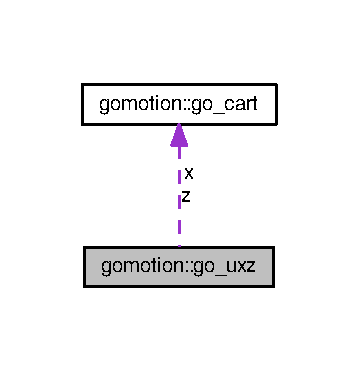
\includegraphics[width=172pt]{d8/de6/structgomotion_1_1go__uxz__coll__graph}
\end{center}
\end{figure}
\subsection*{Data Fields}
\begin{DoxyCompactItemize}
\item 
\hyperlink{structgomotion_1_1go__cart}{go\-\_\-cart} \hyperlink{structgomotion_1_1go__uxz_a1878a66236a43365991c4e4db1e5e518}{x}
\item 
\hyperlink{structgomotion_1_1go__cart}{go\-\_\-cart} \hyperlink{structgomotion_1_1go__uxz_a4c7bd45717e596a7a9331417d9bcfe83}{z}
\end{DoxyCompactItemize}


\subsection{Detailed Description}
X-\/\-Z vector format. {\itshape x} is a unit vector in the X direction, and {\itshape z} is a unit vector in the Z direction. 

\subsection{Field Documentation}
\hypertarget{structgomotion_1_1go__uxz_a1878a66236a43365991c4e4db1e5e518}{\index{gomotion\-::go\-\_\-uxz@{gomotion\-::go\-\_\-uxz}!x@{x}}
\index{x@{x}!gomotion::go_uxz@{gomotion\-::go\-\_\-uxz}}
\subsubsection[{x}]{\setlength{\rightskip}{0pt plus 5cm}{\bf go\-\_\-cart} gomotion\-::go\-\_\-uxz\-::x}}\label{structgomotion_1_1go__uxz_a1878a66236a43365991c4e4db1e5e518}
\hypertarget{structgomotion_1_1go__uxz_a4c7bd45717e596a7a9331417d9bcfe83}{\index{gomotion\-::go\-\_\-uxz@{gomotion\-::go\-\_\-uxz}!z@{z}}
\index{z@{z}!gomotion::go_uxz@{gomotion\-::go\-\_\-uxz}}
\subsubsection[{z}]{\setlength{\rightskip}{0pt plus 5cm}{\bf go\-\_\-cart} gomotion\-::go\-\_\-uxz\-::z}}\label{structgomotion_1_1go__uxz_a4c7bd45717e596a7a9331417d9bcfe83}


The documentation for this struct was generated from the following file\-:\begin{DoxyCompactItemize}
\item 
/usr/local/michalos/nistfanuc\-\_\-ws/src/gomotion/include/gomotion/\hyperlink{gomath_8h}{gomath.\-h}\end{DoxyCompactItemize}

\hypertarget{structgomotion_1_1go__vel}{\section{gomotion\-:\-:go\-\_\-vel Struct Reference}
\label{structgomotion_1_1go__vel}\index{gomotion\-::go\-\_\-vel@{gomotion\-::go\-\_\-vel}}
}


{\ttfamily \#include $<$gomath.\-h$>$}



Collaboration diagram for gomotion\-:\-:go\-\_\-vel\-:\nopagebreak
\begin{figure}[H]
\begin{center}
\leavevmode
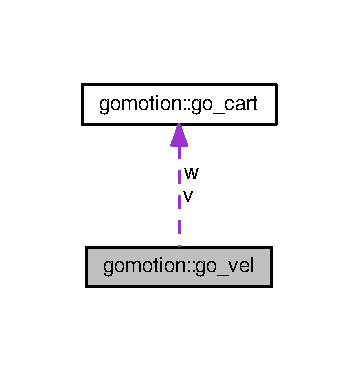
\includegraphics[width=172pt]{dc/dff/structgomotion_1_1go__vel__coll__graph}
\end{center}
\end{figure}
\subsection*{Data Fields}
\begin{DoxyCompactItemize}
\item 
\hyperlink{structgomotion_1_1go__cart}{go\-\_\-cart} \hyperlink{structgomotion_1_1go__vel_ad215a05296181ff4207f75155da830fa}{v}
\item 
\hyperlink{structgomotion_1_1go__cart}{go\-\_\-cart} \hyperlink{structgomotion_1_1go__vel_ae647d5de790b84dad0b91c6f65b998cb}{w}
\end{DoxyCompactItemize}


\subsection{Detailed Description}
A {\itshape \hyperlink{structgomotion_1_1go__vel}{go\-\_\-vel}} represents the linear-\/ and angular velocity vectors of a frame. {\itshape v} is the Cartesian linear velocity vector. {\itshape w} is the Cartesian angular velocity vector, the instantaneous vector about which the frame is rotating. 

\subsection{Field Documentation}
\hypertarget{structgomotion_1_1go__vel_ad215a05296181ff4207f75155da830fa}{\index{gomotion\-::go\-\_\-vel@{gomotion\-::go\-\_\-vel}!v@{v}}
\index{v@{v}!gomotion::go_vel@{gomotion\-::go\-\_\-vel}}
\subsubsection[{v}]{\setlength{\rightskip}{0pt plus 5cm}{\bf go\-\_\-cart} gomotion\-::go\-\_\-vel\-::v}}\label{structgomotion_1_1go__vel_ad215a05296181ff4207f75155da830fa}
\hypertarget{structgomotion_1_1go__vel_ae647d5de790b84dad0b91c6f65b998cb}{\index{gomotion\-::go\-\_\-vel@{gomotion\-::go\-\_\-vel}!w@{w}}
\index{w@{w}!gomotion::go_vel@{gomotion\-::go\-\_\-vel}}
\subsubsection[{w}]{\setlength{\rightskip}{0pt plus 5cm}{\bf go\-\_\-cart} gomotion\-::go\-\_\-vel\-::w}}\label{structgomotion_1_1go__vel_ae647d5de790b84dad0b91c6f65b998cb}


The documentation for this struct was generated from the following file\-:\begin{DoxyCompactItemize}
\item 
/usr/local/michalos/nistfanuc\-\_\-ws/src/gomotion/include/gomotion/\hyperlink{gomath_8h}{gomath.\-h}\end{DoxyCompactItemize}

\hypertarget{structgomotion_1_1go__xyz}{\section{gomotion\-:\-:go\-\_\-xyz Struct Reference}
\label{structgomotion_1_1go__xyz}\index{gomotion\-::go\-\_\-xyz@{gomotion\-::go\-\_\-xyz}}
}


{\ttfamily \#include $<$gomath.\-h$>$}

\subsection*{Data Fields}
\begin{DoxyCompactItemize}
\item 
\hyperlink{gotypes_8h_afd666a2393eebd71ee455846ac9def9b}{go\-\_\-real} \hyperlink{structgomotion_1_1go__xyz_a469ce91ff180b9f80119faaa2e8c4e08}{x}
\item 
\hyperlink{gotypes_8h_afd666a2393eebd71ee455846ac9def9b}{go\-\_\-real} \hyperlink{structgomotion_1_1go__xyz_a452aa1954ffdfb5400356e60394190bd}{y}
\item 
\hyperlink{gotypes_8h_afd666a2393eebd71ee455846ac9def9b}{go\-\_\-real} \hyperlink{structgomotion_1_1go__xyz_a08df5cfb57694ab8caaec6f989b3f739}{z}
\end{DoxyCompactItemize}


\subsection{Detailed Description}
X\-Y\-Z Euler angles. {\itshape x} is the amount of the first rotation around the X axis. {\itshape y} is the amount of the second rotation around the new {\itshape Y} axis. {\itshape z} is the amount of the third rotation around the new {\itshape Z} axis. 

\subsection{Field Documentation}
\hypertarget{structgomotion_1_1go__xyz_a469ce91ff180b9f80119faaa2e8c4e08}{\index{gomotion\-::go\-\_\-xyz@{gomotion\-::go\-\_\-xyz}!x@{x}}
\index{x@{x}!gomotion::go_xyz@{gomotion\-::go\-\_\-xyz}}
\subsubsection[{x}]{\setlength{\rightskip}{0pt plus 5cm}{\bf go\-\_\-real} gomotion\-::go\-\_\-xyz\-::x}}\label{structgomotion_1_1go__xyz_a469ce91ff180b9f80119faaa2e8c4e08}
\hypertarget{structgomotion_1_1go__xyz_a452aa1954ffdfb5400356e60394190bd}{\index{gomotion\-::go\-\_\-xyz@{gomotion\-::go\-\_\-xyz}!y@{y}}
\index{y@{y}!gomotion::go_xyz@{gomotion\-::go\-\_\-xyz}}
\subsubsection[{y}]{\setlength{\rightskip}{0pt plus 5cm}{\bf go\-\_\-real} gomotion\-::go\-\_\-xyz\-::y}}\label{structgomotion_1_1go__xyz_a452aa1954ffdfb5400356e60394190bd}
\hypertarget{structgomotion_1_1go__xyz_a08df5cfb57694ab8caaec6f989b3f739}{\index{gomotion\-::go\-\_\-xyz@{gomotion\-::go\-\_\-xyz}!z@{z}}
\index{z@{z}!gomotion::go_xyz@{gomotion\-::go\-\_\-xyz}}
\subsubsection[{z}]{\setlength{\rightskip}{0pt plus 5cm}{\bf go\-\_\-real} gomotion\-::go\-\_\-xyz\-::z}}\label{structgomotion_1_1go__xyz_a08df5cfb57694ab8caaec6f989b3f739}


The documentation for this struct was generated from the following file\-:\begin{DoxyCompactItemize}
\item 
/usr/local/michalos/nistfanuc\-\_\-ws/src/gomotion/include/gomotion/\hyperlink{gomath_8h}{gomath.\-h}\end{DoxyCompactItemize}

\hypertarget{structgomotion_1_1go__zyx}{\section{gomotion\-:\-:go\-\_\-zyx Struct Reference}
\label{structgomotion_1_1go__zyx}\index{gomotion\-::go\-\_\-zyx@{gomotion\-::go\-\_\-zyx}}
}


{\ttfamily \#include $<$gomath.\-h$>$}

\subsection*{Data Fields}
\begin{DoxyCompactItemize}
\item 
\hyperlink{gotypes_8h_afd666a2393eebd71ee455846ac9def9b}{go\-\_\-real} \hyperlink{structgomotion_1_1go__zyx_aa05f917941bc93c5f19298a1dd16d4f6}{z}
\item 
\hyperlink{gotypes_8h_afd666a2393eebd71ee455846ac9def9b}{go\-\_\-real} \hyperlink{structgomotion_1_1go__zyx_a014cdc80c1901732b84cb1eb65258a82}{y}
\item 
\hyperlink{gotypes_8h_afd666a2393eebd71ee455846ac9def9b}{go\-\_\-real} \hyperlink{structgomotion_1_1go__zyx_aa79612f67b18b68f67cb02bde877c083}{x}
\end{DoxyCompactItemize}


\subsection{Detailed Description}
Z\-Y\-X Euler angles. {\itshape z} is the amount of the first rotation around the Z axis. {\itshape y} is the amount of the second rotation around the new {\itshape Y} axis. {\itshape x} is the amount of the third rotation around the new {\itshape X} axis. 

\subsection{Field Documentation}
\hypertarget{structgomotion_1_1go__zyx_aa79612f67b18b68f67cb02bde877c083}{\index{gomotion\-::go\-\_\-zyx@{gomotion\-::go\-\_\-zyx}!x@{x}}
\index{x@{x}!gomotion::go_zyx@{gomotion\-::go\-\_\-zyx}}
\subsubsection[{x}]{\setlength{\rightskip}{0pt plus 5cm}{\bf go\-\_\-real} gomotion\-::go\-\_\-zyx\-::x}}\label{structgomotion_1_1go__zyx_aa79612f67b18b68f67cb02bde877c083}
\hypertarget{structgomotion_1_1go__zyx_a014cdc80c1901732b84cb1eb65258a82}{\index{gomotion\-::go\-\_\-zyx@{gomotion\-::go\-\_\-zyx}!y@{y}}
\index{y@{y}!gomotion::go_zyx@{gomotion\-::go\-\_\-zyx}}
\subsubsection[{y}]{\setlength{\rightskip}{0pt plus 5cm}{\bf go\-\_\-real} gomotion\-::go\-\_\-zyx\-::y}}\label{structgomotion_1_1go__zyx_a014cdc80c1901732b84cb1eb65258a82}
\hypertarget{structgomotion_1_1go__zyx_aa05f917941bc93c5f19298a1dd16d4f6}{\index{gomotion\-::go\-\_\-zyx@{gomotion\-::go\-\_\-zyx}!z@{z}}
\index{z@{z}!gomotion::go_zyx@{gomotion\-::go\-\_\-zyx}}
\subsubsection[{z}]{\setlength{\rightskip}{0pt plus 5cm}{\bf go\-\_\-real} gomotion\-::go\-\_\-zyx\-::z}}\label{structgomotion_1_1go__zyx_aa05f917941bc93c5f19298a1dd16d4f6}


The documentation for this struct was generated from the following file\-:\begin{DoxyCompactItemize}
\item 
/usr/local/michalos/nistfanuc\-\_\-ws/src/gomotion/include/gomotion/\hyperlink{gomath_8h}{gomath.\-h}\end{DoxyCompactItemize}

\hypertarget{structgomotion_1_1go__zyz}{\section{gomotion\-:\-:go\-\_\-zyz Struct Reference}
\label{structgomotion_1_1go__zyz}\index{gomotion\-::go\-\_\-zyz@{gomotion\-::go\-\_\-zyz}}
}


{\ttfamily \#include $<$gomath.\-h$>$}

\subsection*{Data Fields}
\begin{DoxyCompactItemize}
\item 
\hyperlink{gotypes_8h_afd666a2393eebd71ee455846ac9def9b}{go\-\_\-real} \hyperlink{structgomotion_1_1go__zyz_a87a0a9e59da539abece916a52c8b3d28}{z}
\item 
\hyperlink{gotypes_8h_afd666a2393eebd71ee455846ac9def9b}{go\-\_\-real} \hyperlink{structgomotion_1_1go__zyz_a05cbc6e6ea8660a5d3e64eedea4e9fb7}{y}
\item 
\hyperlink{gotypes_8h_afd666a2393eebd71ee455846ac9def9b}{go\-\_\-real} \hyperlink{structgomotion_1_1go__zyz_a43a807cde8f59f25403e282390331001}{zp}
\end{DoxyCompactItemize}


\subsection{Detailed Description}
Z\-Y\-Z Euler angles. {\itshape z} is the amount of the first rotation around the Z axis. {\itshape y} is the amount of the second rotation around the new {\itshape Y} axis. {\itshape zp} is the amount of the third rotation around the new {\itshape Z} axis. 

\subsection{Field Documentation}
\hypertarget{structgomotion_1_1go__zyz_a05cbc6e6ea8660a5d3e64eedea4e9fb7}{\index{gomotion\-::go\-\_\-zyz@{gomotion\-::go\-\_\-zyz}!y@{y}}
\index{y@{y}!gomotion::go_zyz@{gomotion\-::go\-\_\-zyz}}
\subsubsection[{y}]{\setlength{\rightskip}{0pt plus 5cm}{\bf go\-\_\-real} gomotion\-::go\-\_\-zyz\-::y}}\label{structgomotion_1_1go__zyz_a05cbc6e6ea8660a5d3e64eedea4e9fb7}
\hypertarget{structgomotion_1_1go__zyz_a87a0a9e59da539abece916a52c8b3d28}{\index{gomotion\-::go\-\_\-zyz@{gomotion\-::go\-\_\-zyz}!z@{z}}
\index{z@{z}!gomotion::go_zyz@{gomotion\-::go\-\_\-zyz}}
\subsubsection[{z}]{\setlength{\rightskip}{0pt plus 5cm}{\bf go\-\_\-real} gomotion\-::go\-\_\-zyz\-::z}}\label{structgomotion_1_1go__zyz_a87a0a9e59da539abece916a52c8b3d28}
\hypertarget{structgomotion_1_1go__zyz_a43a807cde8f59f25403e282390331001}{\index{gomotion\-::go\-\_\-zyz@{gomotion\-::go\-\_\-zyz}!zp@{zp}}
\index{zp@{zp}!gomotion::go_zyz@{gomotion\-::go\-\_\-zyz}}
\subsubsection[{zp}]{\setlength{\rightskip}{0pt plus 5cm}{\bf go\-\_\-real} gomotion\-::go\-\_\-zyz\-::zp}}\label{structgomotion_1_1go__zyz_a43a807cde8f59f25403e282390331001}


The documentation for this struct was generated from the following file\-:\begin{DoxyCompactItemize}
\item 
/usr/local/michalos/nistfanuc\-\_\-ws/src/gomotion/include/gomotion/\hyperlink{gomath_8h}{gomath.\-h}\end{DoxyCompactItemize}

\hypertarget{classgomotion_1_1_go_motion}{\section{gomotion\-:\-:Go\-Motion Class Reference}
\label{classgomotion_1_1_go_motion}\index{gomotion\-::\-Go\-Motion@{gomotion\-::\-Go\-Motion}}
}


{\ttfamily \#include $<$gomove.\-h$>$}

\subsection*{Protected Attributes}
\begin{DoxyCompactItemize}
\item 
boost\-::shared\-\_\-ptr\\*
$<$ \hyperlink{structgomotion_1_1go__motion__interface}{go\-\_\-motion\-\_\-interface} $>$ \hyperlink{classgomotion_1_1_go_motion_a9d42007f05e5b2db5e423eb592520f55}{pgm}
\end{DoxyCompactItemize}


\subsection{Field Documentation}
\hypertarget{classgomotion_1_1_go_motion_a9d42007f05e5b2db5e423eb592520f55}{\index{gomotion\-::\-Go\-Motion@{gomotion\-::\-Go\-Motion}!pgm@{pgm}}
\index{pgm@{pgm}!gomotion::GoMotion@{gomotion\-::\-Go\-Motion}}
\subsubsection[{pgm}]{\setlength{\rightskip}{0pt plus 5cm}boost\-::shared\-\_\-ptr$<${\bf go\-\_\-motion\-\_\-interface}$>$ gomotion\-::\-Go\-Motion\-::pgm\hspace{0.3cm}{\ttfamily [protected]}}}\label{classgomotion_1_1_go_motion_a9d42007f05e5b2db5e423eb592520f55}


The documentation for this class was generated from the following files\-:\begin{DoxyCompactItemize}
\item 
/usr/local/michalos/nistfanuc\-\_\-ws/src/gomotion/include/gomotion/\hyperlink{gomove_8h}{gomove.\-h}\item 
/usr/local/michalos/nistfanuc\-\_\-ws/src/gomotion/src/\hyperlink{gomove_8cpp}{gomove.\-cpp}\end{DoxyCompactItemize}

\hypertarget{structgomotion_1_1_go_motion_params}{\section{gomotion\-:\-:Go\-Motion\-Params Struct Reference}
\label{structgomotion_1_1_go_motion_params}\index{gomotion\-::\-Go\-Motion\-Params@{gomotion\-::\-Go\-Motion\-Params}}
}


{\ttfamily \#include $<$gomove.\-h$>$}

\subsection*{Data Fields}
\begin{DoxyCompactItemize}
\item 
double \hyperlink{structgomotion_1_1_go_motion_params_a84993ded24232568329b81331e4b09db}{vel}
\item 
double \hyperlink{structgomotion_1_1_go_motion_params_ab527b270eae069c523e3c16135a587fd}{acc}
\item 
double \hyperlink{structgomotion_1_1_go_motion_params_a82304cfd33f8bcb9c9f0eddf9904c8da}{jerk}
\end{DoxyCompactItemize}


\subsection{Field Documentation}
\hypertarget{structgomotion_1_1_go_motion_params_ab527b270eae069c523e3c16135a587fd}{\index{gomotion\-::\-Go\-Motion\-Params@{gomotion\-::\-Go\-Motion\-Params}!acc@{acc}}
\index{acc@{acc}!gomotion::GoMotionParams@{gomotion\-::\-Go\-Motion\-Params}}
\subsubsection[{acc}]{\setlength{\rightskip}{0pt plus 5cm}double gomotion\-::\-Go\-Motion\-Params\-::acc}}\label{structgomotion_1_1_go_motion_params_ab527b270eae069c523e3c16135a587fd}
\hypertarget{structgomotion_1_1_go_motion_params_a82304cfd33f8bcb9c9f0eddf9904c8da}{\index{gomotion\-::\-Go\-Motion\-Params@{gomotion\-::\-Go\-Motion\-Params}!jerk@{jerk}}
\index{jerk@{jerk}!gomotion::GoMotionParams@{gomotion\-::\-Go\-Motion\-Params}}
\subsubsection[{jerk}]{\setlength{\rightskip}{0pt plus 5cm}double gomotion\-::\-Go\-Motion\-Params\-::jerk}}\label{structgomotion_1_1_go_motion_params_a82304cfd33f8bcb9c9f0eddf9904c8da}
\hypertarget{structgomotion_1_1_go_motion_params_a84993ded24232568329b81331e4b09db}{\index{gomotion\-::\-Go\-Motion\-Params@{gomotion\-::\-Go\-Motion\-Params}!vel@{vel}}
\index{vel@{vel}!gomotion::GoMotionParams@{gomotion\-::\-Go\-Motion\-Params}}
\subsubsection[{vel}]{\setlength{\rightskip}{0pt plus 5cm}double gomotion\-::\-Go\-Motion\-Params\-::vel}}\label{structgomotion_1_1_go_motion_params_a84993ded24232568329b81331e4b09db}


The documentation for this struct was generated from the following file\-:\begin{DoxyCompactItemize}
\item 
/usr/local/michalos/nistfanuc\-\_\-ws/src/gomotion/include/gomotion/\hyperlink{gomove_8h}{gomove.\-h}\end{DoxyCompactItemize}

\hypertarget{structgomotion_1_1points}{\section{gomotion\-:\-:points Struct Reference}
\label{structgomotion_1_1points}\index{gomotion\-::points@{gomotion\-::points}}
}


This structure holds the points to be interpolated.  




{\ttfamily \#include $<$gointerp.\-h$>$}

\subsection*{Data Fields}
\begin{DoxyCompactItemize}
\item 
\hyperlink{gotypes_8h_afd666a2393eebd71ee455846ac9def9b}{go\-\_\-real} \hyperlink{structgomotion_1_1points_a32050509c895b3df0be8f0968d61e5cf}{p} \mbox{[}\hyperlink{namespacegomotion_ada59e79a297fc10f2dbc85e4777fa4aea0d345844cda261ed2253d7fc9404e2ef}{C\-O\-E\-F\-F\-\_\-\-M\-A\-X}\mbox{]}
\end{DoxyCompactItemize}


\subsection{Detailed Description}
This structure holds the points to be interpolated. 

See notes below for how to fill the p\mbox{[}\mbox{]} array for the particular type of interpolation. 

\subsection{Field Documentation}
\hypertarget{structgomotion_1_1points_a32050509c895b3df0be8f0968d61e5cf}{\index{gomotion\-::points@{gomotion\-::points}!p@{p}}
\index{p@{p}!gomotion::points@{gomotion\-::points}}
\subsubsection[{p}]{\setlength{\rightskip}{0pt plus 5cm}{\bf go\-\_\-real} gomotion\-::points\-::p\mbox{[}{\bf C\-O\-E\-F\-F\-\_\-\-M\-A\-X}\mbox{]}}}\label{structgomotion_1_1points_a32050509c895b3df0be8f0968d61e5cf}


The documentation for this struct was generated from the following file\-:\begin{DoxyCompactItemize}
\item 
/usr/local/michalos/nistfanuc\-\_\-ws/src/gomotion/include/gomotion/\hyperlink{gointerp_8h}{gointerp.\-h}\end{DoxyCompactItemize}

\chapter{File Documentation}
\hypertarget{gointerp_8h}{\section{/usr/local/michalos/nistfanuc\-\_\-ws/src/gomotion/include/gomotion/gointerp.h File Reference}
\label{gointerp_8h}\index{/usr/local/michalos/nistfanuc\-\_\-ws/src/gomotion/include/gomotion/gointerp.\-h@{/usr/local/michalos/nistfanuc\-\_\-ws/src/gomotion/include/gomotion/gointerp.\-h}}
}
{\ttfamily \#include \char`\"{}gomotion/gotypes.\-h\char`\"{}}\\*
Include dependency graph for gointerp.\-h\-:\nopagebreak
\begin{figure}[H]
\begin{center}
\leavevmode
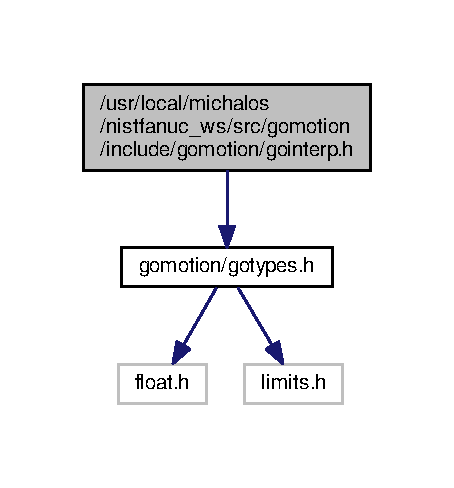
\includegraphics[width=218pt]{d5/d91/gointerp_8h__incl}
\end{center}
\end{figure}
This graph shows which files directly or indirectly include this file\-:\nopagebreak
\begin{figure}[H]
\begin{center}
\leavevmode
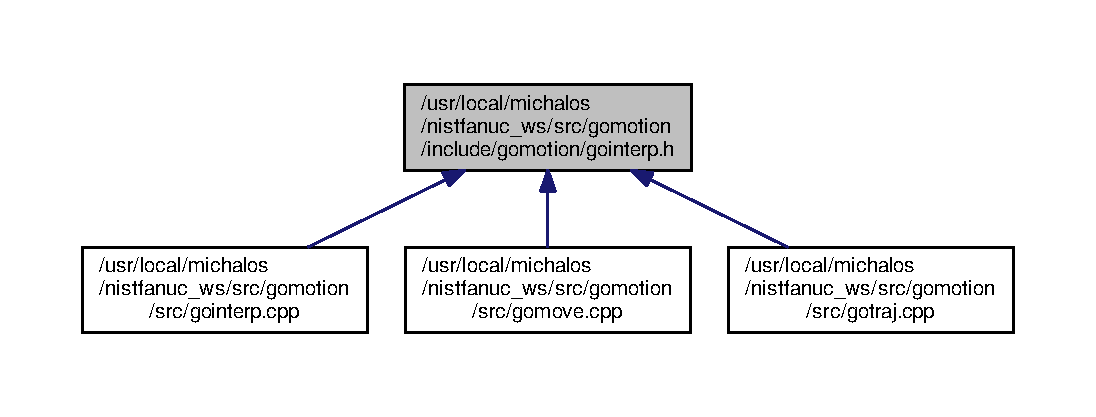
\includegraphics[width=350pt]{d1/df3/gointerp_8h__dep__incl}
\end{center}
\end{figure}
\subsection*{Data Structures}
\begin{DoxyCompactItemize}
\item 
struct \hyperlink{structgomotion_1_1points}{gomotion\-::points}
\begin{DoxyCompactList}\small\item\em This structure holds the points to be interpolated. \end{DoxyCompactList}\item 
struct \hyperlink{structgomotion_1_1coeff}{gomotion\-::coeff}
\begin{DoxyCompactList}\small\item\em This structure holds the polynomial coefficients. \end{DoxyCompactList}\item 
class \hyperlink{classgomotion_1_1go__interp}{gomotion\-::go\-\_\-interp}
\begin{DoxyCompactList}\small\item\em The interpolator structure. \end{DoxyCompactList}\end{DoxyCompactItemize}
\subsection*{Namespaces}
\begin{DoxyCompactItemize}
\item 
\hyperlink{namespacegomotion}{gomotion}
\end{DoxyCompactItemize}
\subsection*{Enumerations}
\begin{DoxyCompactItemize}
\item 
enum \{ \hyperlink{namespacegomotion_ada59e79a297fc10f2dbc85e4777fa4aea0d345844cda261ed2253d7fc9404e2ef}{gomotion\-::\-C\-O\-E\-F\-F\-\_\-\-M\-A\-X} = 6
 \}
\begin{DoxyCompactList}\small\item\em How many coefficients we support, one more than max polynomial degree. \end{DoxyCompactList}\end{DoxyCompactItemize}

\hypertarget{gomath_8h}{\section{/usr/local/michalos/nistfanuc\-\_\-ws/src/gomotion/include/gomotion/gomath.h File Reference}
\label{gomath_8h}\index{/usr/local/michalos/nistfanuc\-\_\-ws/src/gomotion/include/gomotion/gomath.\-h@{/usr/local/michalos/nistfanuc\-\_\-ws/src/gomotion/include/gomotion/gomath.\-h}}
}


Declarations for pose math functions.  


{\ttfamily \#include $<$stddef.\-h$>$}\\*
{\ttfamily \#include $<$math.\-h$>$}\\*
{\ttfamily \#include $<$float.\-h$>$}\\*
{\ttfamily \#include \char`\"{}gomotion/gotypes.\-h\char`\"{}}\\*
Include dependency graph for gomath.\-h\-:\nopagebreak
\begin{figure}[H]
\begin{center}
\leavevmode
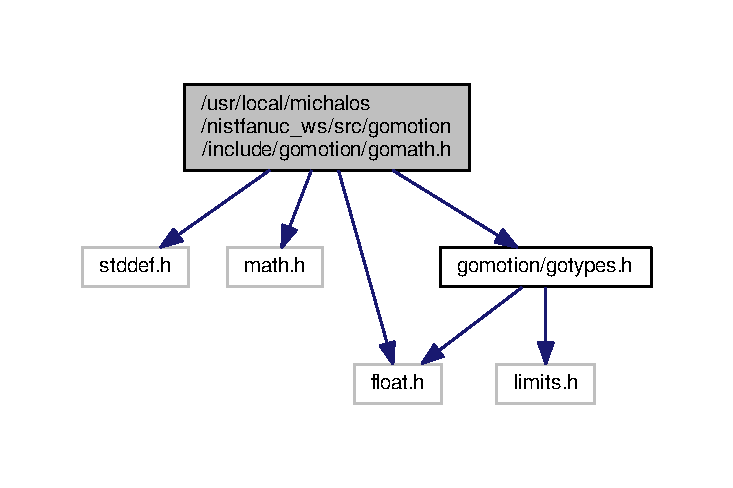
\includegraphics[width=350pt]{d2/d73/gomath_8h__incl}
\end{center}
\end{figure}
This graph shows which files directly or indirectly include this file\-:\nopagebreak
\begin{figure}[H]
\begin{center}
\leavevmode
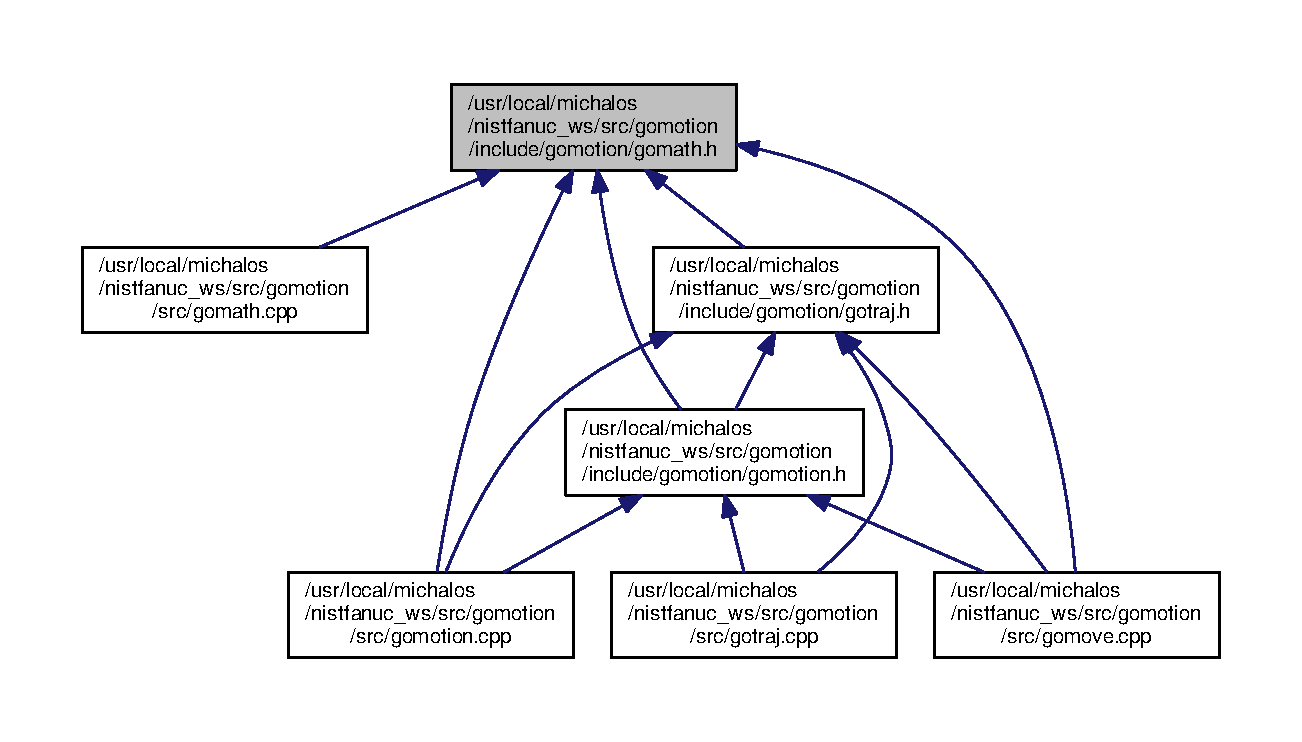
\includegraphics[width=350pt]{de/d60/gomath_8h__dep__incl}
\end{center}
\end{figure}
\subsection*{Data Structures}
\begin{DoxyCompactItemize}
\item 
struct \hyperlink{structgomotion_1_1go__cart}{gomotion\-::go\-\_\-cart}
\item 
struct \hyperlink{structgomotion_1_1go__sph}{gomotion\-::go\-\_\-sph}
\item 
struct \hyperlink{structgomotion_1_1go__cyl}{gomotion\-::go\-\_\-cyl}
\item 
struct \hyperlink{structgomotion_1_1go__rvec}{gomotion\-::go\-\_\-rvec}
\item 
struct \hyperlink{structgomotion_1_1go__mat}{gomotion\-::go\-\_\-mat}
\item 
struct \hyperlink{structgomotion_1_1go__quat}{gomotion\-::go\-\_\-quat}
\item 
struct \hyperlink{structgomotion_1_1go__zyz}{gomotion\-::go\-\_\-zyz}
\item 
struct \hyperlink{structgomotion_1_1go__zyx}{gomotion\-::go\-\_\-zyx}
\item 
struct \hyperlink{structgomotion_1_1go__xyz}{gomotion\-::go\-\_\-xyz}
\item 
struct \hyperlink{structgomotion_1_1go__rpy}{gomotion\-::go\-\_\-rpy}
\item 
struct \hyperlink{structgomotion_1_1go__uxz}{gomotion\-::go\-\_\-uxz}
\item 
struct \hyperlink{structgomotion_1_1go__pose}{gomotion\-::go\-\_\-pose}
\item 
struct \hyperlink{structgomotion_1_1go__vel}{gomotion\-::go\-\_\-vel}
\item 
struct \hyperlink{structgomotion_1_1go__hom}{gomotion\-::go\-\_\-hom}
\item 
struct \hyperlink{structgomotion_1_1go__line}{gomotion\-::go\-\_\-line}
\item 
struct \hyperlink{structgomotion_1_1go__plane}{gomotion\-::go\-\_\-plane}
\item 
struct \hyperlink{structgomotion_1_1go__matrix}{gomotion\-::go\-\_\-matrix}
\item 
struct \hyperlink{structgomotion_1_1go__dh}{gomotion\-::go\-\_\-dh}
\item 
struct \hyperlink{structgomotion_1_1go__pk}{gomotion\-::go\-\_\-pk}
\item 
struct \hyperlink{structgomotion_1_1go__pp}{gomotion\-::go\-\_\-pp}
\item 
struct \hyperlink{structgomotion_1_1go__body}{gomotion\-::go\-\_\-body}
\item 
struct \hyperlink{structgomotion_1_1go__link}{gomotion\-::go\-\_\-link}
\item 
struct \hyperlink{structgomotion_1_1go__complex}{gomotion\-::go\-\_\-complex}
\item 
struct \hyperlink{structgomotion_1_1go__quadratic}{gomotion\-::go\-\_\-quadratic}
\item 
struct \hyperlink{structgomotion_1_1go__cubic}{gomotion\-::go\-\_\-cubic}
\item 
struct \hyperlink{structgomotion_1_1go__quartic}{gomotion\-::go\-\_\-quartic}
\end{DoxyCompactItemize}
\subsection*{Namespaces}
\begin{DoxyCompactItemize}
\item 
\hyperlink{namespacegomotion}{gomotion}
\end{DoxyCompactItemize}
\subsection*{Macros}
\begin{DoxyCompactItemize}
\item 
\#define \hyperlink{gomath_8h_a073619c46f05f2b4180948f5e67328aa}{go\-\_\-sq}(x)~((x)$\ast$(x))
\item 
\#define \hyperlink{gomath_8h_a7b945d7ec90e4d34073e15a23b26dc11}{go\-\_\-cub}(x)~((x)$\ast$(x)$\ast$(x))
\item 
\#define \hyperlink{gomath_8h_a8f92c90d4eca20e4519c3cce423c0b14}{go\-\_\-qua}(x)~((x)$\ast$(x)$\ast$(x)$\ast$(x))
\item 
\#define \hyperlink{gomath_8h_a52cc993e19bca5c01e117b6bd840de0d}{G\-O\-\_\-\-P\-I}~3.\-14159265358979323846
\item 
\#define \hyperlink{gomath_8h_aa826db35de339d014c00c259b4b932f5}{G\-O\-\_\-2\-\_\-\-P\-I}~(2.\-0$\ast$\hyperlink{gomath_8h_a52cc993e19bca5c01e117b6bd840de0d}{G\-O\-\_\-\-P\-I})
\item 
\#define \hyperlink{gomath_8h_a75f159bb4031d698794771824e92540a}{G\-O\-\_\-\-P\-I\-\_\-2}~1.\-57079632679489661923
\item 
\#define \hyperlink{gomath_8h_ad02346b33ded3bb4f6a3d795f372f0c2}{G\-O\-\_\-\-P\-I\-\_\-4}~0.\-78539816339744830962
\item 
\#define \hyperlink{gomath_8h_ab49e228fd567903d32654564c81a606f}{G\-O\-\_\-\-T\-O\-\_\-\-D\-E\-G}(rad)~((rad)$\ast$57.\-295779513082323)
\item 
\#define \hyperlink{gomath_8h_a257fd1bdbb4294c1bf1d2c34bfeaba42}{G\-O\-\_\-\-T\-O\-\_\-\-R\-A\-D}(deg)~((deg)$\ast$0.\-0174532925199432952)
\item 
\#define \hyperlink{gomath_8h_ab72173c33a8f16e8ecec3b552d2f5ba2}{G\-O\-\_\-\-T\-R\-A\-N\-\_\-\-C\-L\-O\-S\-E}(x, y)~(fabs((x)-\/(y)) $<$ \hyperlink{gotypes_8h_a565feef8b688896bae12bba085027170}{G\-O\-\_\-\-R\-E\-A\-L\-\_\-\-E\-P\-S\-I\-L\-O\-N})
\item 
\#define \hyperlink{gomath_8h_a9a43e1f84698a4a207443d40f885ecd6}{G\-O\-\_\-\-T\-R\-A\-N\-\_\-\-S\-M\-A\-L\-L}(x)~(fabs(x) $<$ \hyperlink{gotypes_8h_a565feef8b688896bae12bba085027170}{G\-O\-\_\-\-R\-E\-A\-L\-\_\-\-E\-P\-S\-I\-L\-O\-N})
\item 
\#define \hyperlink{gomath_8h_a05cedbcc55d6939a67c17c1e3b71d488}{G\-O\-\_\-\-R\-O\-T\-\_\-\-C\-L\-O\-S\-E}(x, y)~(fabs((x)-\/(y)) $<$ \hyperlink{gotypes_8h_a565feef8b688896bae12bba085027170}{G\-O\-\_\-\-R\-E\-A\-L\-\_\-\-E\-P\-S\-I\-L\-O\-N})
\item 
\#define \hyperlink{gomath_8h_a94c8163e4f01c4adf33baa8eb995433d}{G\-O\-\_\-\-R\-O\-T\-\_\-\-S\-M\-A\-L\-L}(x)~(fabs(x) $<$ \hyperlink{gotypes_8h_a565feef8b688896bae12bba085027170}{G\-O\-\_\-\-R\-E\-A\-L\-\_\-\-E\-P\-S\-I\-L\-O\-N})
\item 
\#define \hyperlink{gomath_8h_a2dbfee2dbb4523cc08316fd2080d4299}{G\-O\-\_\-\-C\-L\-O\-S\-E}(x, y)~(fabs((x)-\/(y)) $<$ \hyperlink{gotypes_8h_a565feef8b688896bae12bba085027170}{G\-O\-\_\-\-R\-E\-A\-L\-\_\-\-E\-P\-S\-I\-L\-O\-N})
\item 
\#define \hyperlink{gomath_8h_acccd2104a7cee68bf586057facfea5d5}{G\-O\-\_\-\-S\-M\-A\-L\-L}(x)~(fabs(x) $<$ \hyperlink{gotypes_8h_a565feef8b688896bae12bba085027170}{G\-O\-\_\-\-R\-E\-A\-L\-\_\-\-E\-P\-S\-I\-L\-O\-N})
\item 
\#define \hyperlink{gomath_8h_ac29f0652fd2215fe0713d7b473a72343}{G\-O\-\_\-\-M\-A\-T\-R\-I\-X\-\_\-\-D\-E\-C\-L\-A\-R\-E}(M, Mspace, \-\_\-rows, \-\_\-cols)
\item 
\#define \hyperlink{gomath_8h_a83429625babfbf9dd959fda081191b44}{I\-S\-I\-Z\-E\-O\-F}(x)~((int) sizeof(x))
\item 
\#define \hyperlink{gomath_8h_a68b54c3bb7c9bbf14f68336cf474a5a3}{go\-\_\-matrix\-\_\-init}(M, Mspace, \-\_\-rows, \-\_\-cols)
\item 
\#define \hyperlink{gomath_8h_a0d434996426b71e86dbff3ec483ee5f9}{go\-\_\-body\-\_\-init}(b)
\item 
\#define \hyperlink{gomath_8h_a927bcd9bd678cacb06596c4e9aad7eb4}{go\-\_\-body\-\_\-copy}(src, dst)
\item 
\#define \hyperlink{gomath_8h_a7fbee1dbcd46c80fe1b6f67550b4d1d3}{go\-\_\-link\-\_\-to\-\_\-string}(L)
\end{DoxyCompactItemize}
\subsection*{Typedefs}
\begin{DoxyCompactItemize}
\item 
typedef \hyperlink{gotypes_8h_afd666a2393eebd71ee455846ac9def9b}{go\-\_\-real} \hyperlink{namespacegomotion_a5739eac588a6a458ed9258bae0a3fc80}{gomotion\-::go\-\_\-vector}
\end{DoxyCompactItemize}
\subsection*{Enumerations}
\begin{DoxyCompactItemize}
\item 
enum \{ \hyperlink{namespacegomotion_a5b5a03fc09c09e262c6941325f7beb17afd19d6aee8f10a912a656a2e01650b62}{gomotion\-::\-G\-O\-\_\-\-L\-I\-N\-K\-\_\-\-D\-H} = 1, 
\hyperlink{namespacegomotion_a5b5a03fc09c09e262c6941325f7beb17a7b78cd6a637ea7ae037ec521ef34b8ab}{gomotion\-::\-G\-O\-\_\-\-L\-I\-N\-K\-\_\-\-P\-K}, 
\hyperlink{namespacegomotion_a5b5a03fc09c09e262c6941325f7beb17acbaa1fd4ed04f6ed93cc5296baaf6b78}{gomotion\-::\-G\-O\-\_\-\-L\-I\-N\-K\-\_\-\-P\-P}
 \}
\end{DoxyCompactItemize}
\subsection*{Functions}
\begin{DoxyCompactItemize}
\item 
void \hyperlink{namespacegomotion_a085a19f481a6f3f319f644b6dc5fca4b}{gomotion\-::go\-\_\-sincos} (\hyperlink{gotypes_8h_afd666a2393eebd71ee455846ac9def9b}{go\-\_\-real} t, \hyperlink{gotypes_8h_afd666a2393eebd71ee455846ac9def9b}{go\-\_\-real} $\ast$s, \hyperlink{gotypes_8h_afd666a2393eebd71ee455846ac9def9b}{go\-\_\-real} $\ast$c)
\item 
\hyperlink{gotypes_8h_afd666a2393eebd71ee455846ac9def9b}{go\-\_\-real} \hyperlink{namespacegomotion_a11b672dbc5c887c373bd7421c4d74744}{gomotion\-::go\-\_\-cbrt} (\hyperlink{gotypes_8h_afd666a2393eebd71ee455846ac9def9b}{go\-\_\-real} x)
\item 
\hyperlink{gotypes_8h_a55d48b38cd959f63c7e8db8337a9792a}{go\-\_\-result} \hyperlink{namespacegomotion_a8bf33ee1ceabf5861cb6d8f7fe685880}{gomotion\-::go\-\_\-asines} (\hyperlink{gotypes_8h_afd666a2393eebd71ee455846ac9def9b}{go\-\_\-real} s, \hyperlink{gotypes_8h_afd666a2393eebd71ee455846ac9def9b}{go\-\_\-real} $\ast$asp, \hyperlink{gotypes_8h_afd666a2393eebd71ee455846ac9def9b}{go\-\_\-real} $\ast$asn)
\item 
\hyperlink{gotypes_8h_a55d48b38cd959f63c7e8db8337a9792a}{go\-\_\-result} \hyperlink{namespacegomotion_a763dfb5f3ead47a101119bc4ef7a9822}{gomotion\-::go\-\_\-acoses} (\hyperlink{gotypes_8h_afd666a2393eebd71ee455846ac9def9b}{go\-\_\-real} c, \hyperlink{gotypes_8h_afd666a2393eebd71ee455846ac9def9b}{go\-\_\-real} $\ast$acp, \hyperlink{gotypes_8h_afd666a2393eebd71ee455846ac9def9b}{go\-\_\-real} $\ast$acn)
\item 
\hyperlink{gotypes_8h_a55d48b38cd959f63c7e8db8337a9792a}{go\-\_\-result} \hyperlink{namespacegomotion_a6af3a55c31db0c4b47aa157de48ae829}{gomotion\-::go\-\_\-atans} (\hyperlink{gotypes_8h_afd666a2393eebd71ee455846ac9def9b}{go\-\_\-real} t, \hyperlink{gotypes_8h_afd666a2393eebd71ee455846ac9def9b}{go\-\_\-real} $\ast$atp, \hyperlink{gotypes_8h_afd666a2393eebd71ee455846ac9def9b}{go\-\_\-real} $\ast$atn)
\item 
go\-\_\-pose \hyperlink{namespacegomotion_a71730b5182346e2fe15337c358013fca}{gomotion\-::go\-\_\-pose\-\_\-this} (\hyperlink{gotypes_8h_afd666a2393eebd71ee455846ac9def9b}{go\-\_\-real} x, \hyperlink{gotypes_8h_afd666a2393eebd71ee455846ac9def9b}{go\-\_\-real} y, \hyperlink{gotypes_8h_afd666a2393eebd71ee455846ac9def9b}{go\-\_\-real} z, \hyperlink{gotypes_8h_afd666a2393eebd71ee455846ac9def9b}{go\-\_\-real} rs, \hyperlink{gotypes_8h_afd666a2393eebd71ee455846ac9def9b}{go\-\_\-real} rx, \hyperlink{gotypes_8h_afd666a2393eebd71ee455846ac9def9b}{go\-\_\-real} ry, \hyperlink{gotypes_8h_afd666a2393eebd71ee455846ac9def9b}{go\-\_\-real} rz)
\item 
go\-\_\-cart \hyperlink{namespacegomotion_aadcf705cf7a6b2a33fb3fb65f5b1a517}{gomotion\-::go\-\_\-cart\-\_\-zero} (void)
\item 
go\-\_\-quat \hyperlink{namespacegomotion_abfb9197b7cceb73fdd68bad553cba624}{gomotion\-::go\-\_\-quat\-\_\-identity} (void)
\item 
go\-\_\-pose \hyperlink{namespacegomotion_ab1257b2f7a291d528ea01466abff5ac8}{gomotion\-::go\-\_\-pose\-\_\-identity} (void)
\item 
\hyperlink{gotypes_8h_a55d48b38cd959f63c7e8db8337a9792a}{go\-\_\-result} \hyperlink{namespacegomotion_aac937b55b391d0b7565719d301389bc6}{gomotion\-::go\-\_\-line\-\_\-from\-\_\-point\-\_\-direction} (const go\-\_\-cart $\ast$point, const go\-\_\-cart $\ast$direction, go\-\_\-line $\ast$line)
\item 
\hyperlink{gotypes_8h_a55d48b38cd959f63c7e8db8337a9792a}{go\-\_\-result} \hyperlink{namespacegomotion_a13ea203461728105546fe4af4083f6ba}{gomotion\-::go\-\_\-line\-\_\-from\-\_\-points} (const go\-\_\-cart $\ast$point1, const go\-\_\-cart $\ast$point2, go\-\_\-line $\ast$line)
\item 
\hyperlink{gotypes_8h_a55d48b38cd959f63c7e8db8337a9792a}{go\-\_\-result} \hyperlink{namespacegomotion_a239960b865134d678928490b91100702}{gomotion\-::go\-\_\-line\-\_\-from\-\_\-planes} (const go\-\_\-plane $\ast$plane1, const go\-\_\-plane $\ast$plane2, go\-\_\-line $\ast$line)
\item 
\hyperlink{gotypes_8h_ae890d9a0ddecc0d3073622cc4312092d}{go\-\_\-flag} \hyperlink{namespacegomotion_a5b409973e65746e7698f0afbcf9183de}{gomotion\-::go\-\_\-line\-\_\-line\-\_\-compare} (const go\-\_\-line $\ast$line1, const go\-\_\-line $\ast$line2)
\item 
\hyperlink{gotypes_8h_a55d48b38cd959f63c7e8db8337a9792a}{go\-\_\-result} \hyperlink{namespacegomotion_a301c198b3225ff73ad5598c046166a4a}{gomotion\-::go\-\_\-line\-\_\-evaluate} (const go\-\_\-line $\ast$line, \hyperlink{gotypes_8h_afd666a2393eebd71ee455846ac9def9b}{go\-\_\-real} d, go\-\_\-cart $\ast$point)
\item 
\hyperlink{gotypes_8h_a55d48b38cd959f63c7e8db8337a9792a}{go\-\_\-result} \hyperlink{namespacegomotion_a2144eb2d183b1aaf60549d66ae7dfcf6}{gomotion\-::go\-\_\-point\-\_\-line\-\_\-distance} (const go\-\_\-cart $\ast$point, const go\-\_\-line $\ast$line, \hyperlink{gotypes_8h_afd666a2393eebd71ee455846ac9def9b}{go\-\_\-real} $\ast$distance)
\item 
\hyperlink{gotypes_8h_a55d48b38cd959f63c7e8db8337a9792a}{go\-\_\-result} \hyperlink{namespacegomotion_a36bd2c5167f64cc51da6bdf3dbdb4116}{gomotion\-::go\-\_\-point\-\_\-line\-\_\-proj} (const go\-\_\-cart $\ast$point, const go\-\_\-line $\ast$line, go\-\_\-cart $\ast$pout)
\item 
\hyperlink{gotypes_8h_a55d48b38cd959f63c7e8db8337a9792a}{go\-\_\-result} \hyperlink{namespacegomotion_a79d749aa4142b2ee2e135f46a6656f21}{gomotion\-::go\-\_\-point\-\_\-plane\-\_\-proj} (const go\-\_\-cart $\ast$point, const go\-\_\-plane $\ast$plane, go\-\_\-cart $\ast$proj)
\item 
\hyperlink{gotypes_8h_a55d48b38cd959f63c7e8db8337a9792a}{go\-\_\-result} \hyperlink{namespacegomotion_a120a912e2b439a904744d980b62867aa}{gomotion\-::go\-\_\-line\-\_\-plane\-\_\-proj} (const go\-\_\-line $\ast$line, const go\-\_\-plane $\ast$plane, go\-\_\-line $\ast$proj)
\item 
\hyperlink{gotypes_8h_a55d48b38cd959f63c7e8db8337a9792a}{go\-\_\-result} \hyperlink{namespacegomotion_abffde2f69bd2e58d2b099558e892661e}{gomotion\-::go\-\_\-plane\-\_\-from\-\_\-point\-\_\-normal} (const go\-\_\-cart $\ast$point, const go\-\_\-cart $\ast$normal, go\-\_\-plane $\ast$plane)
\item 
\hyperlink{gotypes_8h_a55d48b38cd959f63c7e8db8337a9792a}{go\-\_\-result} \hyperlink{namespacegomotion_a62472d69cf3770531052efa51d42d139}{gomotion\-::go\-\_\-plane\-\_\-from\-\_\-abcd} (\hyperlink{gotypes_8h_afd666a2393eebd71ee455846ac9def9b}{go\-\_\-real} A, \hyperlink{gotypes_8h_afd666a2393eebd71ee455846ac9def9b}{go\-\_\-real} B, \hyperlink{gotypes_8h_afd666a2393eebd71ee455846ac9def9b}{go\-\_\-real} C, \hyperlink{gotypes_8h_afd666a2393eebd71ee455846ac9def9b}{go\-\_\-real} D, go\-\_\-plane $\ast$plane)
\item 
\hyperlink{gotypes_8h_a55d48b38cd959f63c7e8db8337a9792a}{go\-\_\-result} \hyperlink{namespacegomotion_aebc299a30f9b6bab3221df9381691a7a}{gomotion\-::go\-\_\-plane\-\_\-from\-\_\-points} (const go\-\_\-cart $\ast$point1, const go\-\_\-cart $\ast$point2, const go\-\_\-cart $\ast$point3, go\-\_\-plane $\ast$plane)
\item 
\hyperlink{gotypes_8h_a55d48b38cd959f63c7e8db8337a9792a}{go\-\_\-result} \hyperlink{namespacegomotion_a3f05dac5f9be2e82ec390a70d03ea058}{gomotion\-::go\-\_\-plane\-\_\-from\-\_\-point\-\_\-line} (const go\-\_\-cart $\ast$point, const go\-\_\-line $\ast$line, go\-\_\-plane $\ast$plane)
\item 
\hyperlink{gotypes_8h_ae890d9a0ddecc0d3073622cc4312092d}{go\-\_\-flag} \hyperlink{namespacegomotion_a522b91008a97b01ef46291dcd5bcb2e0}{gomotion\-::go\-\_\-plane\-\_\-plane\-\_\-compare} (const go\-\_\-plane $\ast$plane1, const go\-\_\-plane $\ast$plane2)
\item 
\hyperlink{gotypes_8h_a55d48b38cd959f63c7e8db8337a9792a}{go\-\_\-result} \hyperlink{namespacegomotion_a9e922da92de4833b51a5867e8fd99cca}{gomotion\-::go\-\_\-point\-\_\-plane\-\_\-distance} (const go\-\_\-cart $\ast$point, const go\-\_\-plane $\ast$plane, \hyperlink{gotypes_8h_afd666a2393eebd71ee455846ac9def9b}{go\-\_\-real} $\ast$distance)
\item 
\hyperlink{gotypes_8h_a55d48b38cd959f63c7e8db8337a9792a}{go\-\_\-result} \hyperlink{namespacegomotion_a45d26171e087d7b1abf3664a127d7006}{gomotion\-::go\-\_\-plane\-\_\-evaluate} (const go\-\_\-plane $\ast$plane, \hyperlink{gotypes_8h_afd666a2393eebd71ee455846ac9def9b}{go\-\_\-real} u, \hyperlink{gotypes_8h_afd666a2393eebd71ee455846ac9def9b}{go\-\_\-real} v, go\-\_\-cart $\ast$point)
\item 
\hyperlink{gotypes_8h_a55d48b38cd959f63c7e8db8337a9792a}{go\-\_\-result} \hyperlink{namespacegomotion_a07b423b2ecb498fbdc2cc810ae52980c}{gomotion\-::go\-\_\-line\-\_\-plane\-\_\-intersect} (const go\-\_\-line $\ast$line, const go\-\_\-plane $\ast$plane, go\-\_\-cart $\ast$point, \hyperlink{gotypes_8h_afd666a2393eebd71ee455846ac9def9b}{go\-\_\-real} $\ast$distance)
\item 
\hyperlink{gotypes_8h_a55d48b38cd959f63c7e8db8337a9792a}{go\-\_\-result} \hyperlink{namespacegomotion_a83b84d0103b59f7ec48a5d50d3633b0d}{gomotion\-::go\-\_\-cart\-\_\-sph\-\_\-convert} (const go\-\_\-cart $\ast$v, go\-\_\-sph $\ast$s)
\item 
\hyperlink{gotypes_8h_a55d48b38cd959f63c7e8db8337a9792a}{go\-\_\-result} \hyperlink{namespacegomotion_a7647c5352af65cc2c74b6ec1543f16dd}{gomotion\-::go\-\_\-cart\-\_\-cyl\-\_\-convert} (const go\-\_\-cart $\ast$v, go\-\_\-cyl $\ast$c)
\item 
\hyperlink{gotypes_8h_a55d48b38cd959f63c7e8db8337a9792a}{go\-\_\-result} \hyperlink{namespacegomotion_a36a8f262d1a993877a8d31f07eff7889}{gomotion\-::go\-\_\-sph\-\_\-cart\-\_\-convert} (const go\-\_\-sph $\ast$s, go\-\_\-cart $\ast$v)
\item 
\hyperlink{gotypes_8h_a55d48b38cd959f63c7e8db8337a9792a}{go\-\_\-result} \hyperlink{namespacegomotion_af03af2d32b5e62c1ead37c2349cc2f46}{gomotion\-::go\-\_\-sph\-\_\-cyl\-\_\-convert} (const go\-\_\-sph $\ast$s, go\-\_\-cyl $\ast$c)
\item 
\hyperlink{gotypes_8h_a55d48b38cd959f63c7e8db8337a9792a}{go\-\_\-result} \hyperlink{namespacegomotion_abeed59a4cd9519af1b4aaed3c116bd39}{gomotion\-::go\-\_\-cyl\-\_\-cart\-\_\-convert} (const go\-\_\-cyl $\ast$c, go\-\_\-cart $\ast$v)
\item 
\hyperlink{gotypes_8h_a55d48b38cd959f63c7e8db8337a9792a}{go\-\_\-result} \hyperlink{namespacegomotion_ab0bdb87e30818c0fb99166f66f04f847}{gomotion\-::go\-\_\-cyl\-\_\-sph\-\_\-convert} (const go\-\_\-cyl $\ast$c, go\-\_\-sph $\ast$s)
\item 
\hyperlink{gotypes_8h_a55d48b38cd959f63c7e8db8337a9792a}{go\-\_\-result} \hyperlink{namespacegomotion_a5241e24d5f0f0202cc947b7abe59c94d}{gomotion\-::go\-\_\-rvec\-\_\-quat\-\_\-convert} (const go\-\_\-rvec $\ast$r, go\-\_\-quat $\ast$q)
\item 
\hyperlink{gotypes_8h_a55d48b38cd959f63c7e8db8337a9792a}{go\-\_\-result} \hyperlink{namespacegomotion_adf77bee641ddc2ab262b5a7c1037b5fb}{gomotion\-::go\-\_\-rvec\-\_\-mat\-\_\-convert} (const go\-\_\-rvec $\ast$r, go\-\_\-mat $\ast$m)
\item 
\hyperlink{gotypes_8h_a55d48b38cd959f63c7e8db8337a9792a}{go\-\_\-result} \hyperlink{namespacegomotion_a55405939228fa6cf1b4e417361e31cf1}{gomotion\-::go\-\_\-rvec\-\_\-zyz\-\_\-convert} (const go\-\_\-rvec $\ast$rvec, go\-\_\-zyz $\ast$zyz)
\item 
\hyperlink{gotypes_8h_a55d48b38cd959f63c7e8db8337a9792a}{go\-\_\-result} \hyperlink{namespacegomotion_a1ba2b7da6d49b4ead52117a0d424cbb0}{gomotion\-::go\-\_\-rvec\-\_\-zyx\-\_\-convert} (const go\-\_\-rvec $\ast$rvec, go\-\_\-zyx $\ast$zyx)
\item 
\hyperlink{gotypes_8h_a55d48b38cd959f63c7e8db8337a9792a}{go\-\_\-result} \hyperlink{namespacegomotion_a0241f448104df5bf2349d5378c4b0741}{gomotion\-::go\-\_\-rvec\-\_\-xyz\-\_\-convert} (const go\-\_\-rvec $\ast$, go\-\_\-xyz $\ast$)
\item 
\hyperlink{gotypes_8h_a55d48b38cd959f63c7e8db8337a9792a}{go\-\_\-result} \hyperlink{namespacegomotion_a9eec26c29c252c49373f7871e573a3ad}{gomotion\-::go\-\_\-rvec\-\_\-rpy\-\_\-convert} (const go\-\_\-rvec $\ast$r, go\-\_\-rpy $\ast$rpy)
\item 
\hyperlink{gotypes_8h_a55d48b38cd959f63c7e8db8337a9792a}{go\-\_\-result} \hyperlink{namespacegomotion_aba2fc0381e9085e8bedcde7c543a0b1a}{gomotion\-::go\-\_\-quat\-\_\-rvec\-\_\-convert} (const go\-\_\-quat $\ast$q, go\-\_\-rvec $\ast$r)
\item 
\hyperlink{gotypes_8h_a55d48b38cd959f63c7e8db8337a9792a}{go\-\_\-result} \hyperlink{namespacegomotion_adb5fb3eb9abe8e8e6a96ec2c5bdf3857}{gomotion\-::go\-\_\-quat\-\_\-mat\-\_\-convert} (const go\-\_\-quat $\ast$q, go\-\_\-mat $\ast$m)
\item 
\hyperlink{gotypes_8h_a55d48b38cd959f63c7e8db8337a9792a}{go\-\_\-result} \hyperlink{namespacegomotion_a7465dd12350d9c9fc9b59ef619796071}{gomotion\-::go\-\_\-quat\-\_\-zyz\-\_\-convert} (const go\-\_\-quat $\ast$q, go\-\_\-zyz $\ast$zyz)
\item 
\hyperlink{gotypes_8h_a55d48b38cd959f63c7e8db8337a9792a}{go\-\_\-result} \hyperlink{namespacegomotion_a4e32c0da5973b4a837a29bcd4f46a166}{gomotion\-::go\-\_\-quat\-\_\-zyx\-\_\-convert} (const go\-\_\-quat $\ast$q, go\-\_\-zyx $\ast$zyx)
\item 
\hyperlink{gotypes_8h_a55d48b38cd959f63c7e8db8337a9792a}{go\-\_\-result} \hyperlink{namespacegomotion_a163a10f7d3fef90a12477d42d48e0a3f}{gomotion\-::go\-\_\-quat\-\_\-xyz\-\_\-convert} (const go\-\_\-quat $\ast$, go\-\_\-xyz $\ast$)
\item 
\hyperlink{gotypes_8h_a55d48b38cd959f63c7e8db8337a9792a}{go\-\_\-result} \hyperlink{namespacegomotion_a8c4bdba65a6b7ff8b6201e84ddde1fe2}{gomotion\-::go\-\_\-quat\-\_\-rpy\-\_\-convert} (const go\-\_\-quat $\ast$q, go\-\_\-rpy $\ast$rpy)
\item 
\hyperlink{gotypes_8h_a55d48b38cd959f63c7e8db8337a9792a}{go\-\_\-result} \hyperlink{namespacegomotion_a0ece2b09a5698233266153dad1cc1896}{gomotion\-::go\-\_\-mat\-\_\-rvec\-\_\-convert} (const go\-\_\-mat $\ast$m, go\-\_\-rvec $\ast$r)
\item 
\hyperlink{gotypes_8h_a55d48b38cd959f63c7e8db8337a9792a}{go\-\_\-result} \hyperlink{namespacegomotion_a56227bf3fda923a384a50d848d2c2314}{gomotion\-::go\-\_\-mat\-\_\-quat\-\_\-convert} (const go\-\_\-mat $\ast$m, go\-\_\-quat $\ast$q)
\item 
\hyperlink{gotypes_8h_a55d48b38cd959f63c7e8db8337a9792a}{go\-\_\-result} \hyperlink{namespacegomotion_aad03f6a80af4b6d8f8c39e5af91484bc}{gomotion\-::go\-\_\-mat\-\_\-zyz\-\_\-convert} (const go\-\_\-mat $\ast$m, go\-\_\-zyz $\ast$zyz)
\item 
\hyperlink{gotypes_8h_a55d48b38cd959f63c7e8db8337a9792a}{go\-\_\-result} \hyperlink{namespacegomotion_ab6def00d51644dc86a0aad564b029ce3}{gomotion\-::go\-\_\-mat\-\_\-zyx\-\_\-convert} (const go\-\_\-mat $\ast$m, go\-\_\-zyx $\ast$zyx)
\item 
\hyperlink{gotypes_8h_a55d48b38cd959f63c7e8db8337a9792a}{go\-\_\-result} \hyperlink{namespacegomotion_ac8969285bc78a45cc21064577803c758}{gomotion\-::go\-\_\-mat\-\_\-xyz\-\_\-convert} (const go\-\_\-mat $\ast$m, go\-\_\-xyz $\ast$xyz)
\item 
\hyperlink{gotypes_8h_a55d48b38cd959f63c7e8db8337a9792a}{go\-\_\-result} \hyperlink{namespacegomotion_ae3d47ff3b11c3be6ec86196b5acca01f}{gomotion\-::go\-\_\-mat\-\_\-rpy\-\_\-convert} (const go\-\_\-mat $\ast$m, go\-\_\-rpy $\ast$rpy)
\item 
\hyperlink{gotypes_8h_a55d48b38cd959f63c7e8db8337a9792a}{go\-\_\-result} \hyperlink{namespacegomotion_ad53feb4160060f91e636345961c12c1d}{gomotion\-::go\-\_\-zyz\-\_\-rvec\-\_\-convert} (const go\-\_\-zyz $\ast$zyz, go\-\_\-rvec $\ast$r)
\item 
\hyperlink{gotypes_8h_a55d48b38cd959f63c7e8db8337a9792a}{go\-\_\-result} \hyperlink{namespacegomotion_ad0211d9ce3c6f9e8fbbe80a184b15d9e}{gomotion\-::go\-\_\-zyz\-\_\-quat\-\_\-convert} (const go\-\_\-zyz $\ast$zyz, go\-\_\-quat $\ast$q)
\item 
\hyperlink{gotypes_8h_a55d48b38cd959f63c7e8db8337a9792a}{go\-\_\-result} \hyperlink{namespacegomotion_a4d8ad1df8907c07480486bc9284f3cfa}{gomotion\-::go\-\_\-zyz\-\_\-mat\-\_\-convert} (const go\-\_\-zyz $\ast$zyz, go\-\_\-mat $\ast$m)
\item 
\hyperlink{gotypes_8h_a55d48b38cd959f63c7e8db8337a9792a}{go\-\_\-result} \hyperlink{namespacegomotion_a132d8bf451632c63d152a70ac9e55824}{gomotion\-::go\-\_\-zyz\-\_\-zyx\-\_\-convert} (const go\-\_\-zyz $\ast$zyz, go\-\_\-zyx $\ast$zyx)
\item 
\hyperlink{gotypes_8h_a55d48b38cd959f63c7e8db8337a9792a}{go\-\_\-result} \hyperlink{namespacegomotion_a97c3fe1a698a6ab2e62d35ac585ea61d}{gomotion\-::go\-\_\-zyz\-\_\-xyz\-\_\-convert} (const go\-\_\-zyz $\ast$, go\-\_\-xyz $\ast$)
\item 
\hyperlink{gotypes_8h_a55d48b38cd959f63c7e8db8337a9792a}{go\-\_\-result} \hyperlink{namespacegomotion_a186e9aa386fc471351cc8f3d819730f7}{gomotion\-::go\-\_\-zyz\-\_\-rpy\-\_\-convert} (const go\-\_\-zyz $\ast$zyz, go\-\_\-rpy $\ast$rpy)
\item 
\hyperlink{gotypes_8h_a55d48b38cd959f63c7e8db8337a9792a}{go\-\_\-result} \hyperlink{namespacegomotion_a9c449c8dc1828671f0acc40ace796d68}{gomotion\-::go\-\_\-zyx\-\_\-rvec\-\_\-convert} (const go\-\_\-zyx $\ast$zyx, go\-\_\-rvec $\ast$r)
\item 
\hyperlink{gotypes_8h_a55d48b38cd959f63c7e8db8337a9792a}{go\-\_\-result} \hyperlink{namespacegomotion_a0f27fd09f8d74304db6e9ca8185a9623}{gomotion\-::go\-\_\-zyx\-\_\-quat\-\_\-convert} (const go\-\_\-zyx $\ast$zyx, go\-\_\-quat $\ast$q)
\item 
\hyperlink{gotypes_8h_a55d48b38cd959f63c7e8db8337a9792a}{go\-\_\-result} \hyperlink{namespacegomotion_a70010a8b112dc746b53c5e8e6afa9637}{gomotion\-::go\-\_\-zyx\-\_\-mat\-\_\-convert} (const go\-\_\-zyx $\ast$zyx, go\-\_\-mat $\ast$m)
\item 
\hyperlink{gotypes_8h_a55d48b38cd959f63c7e8db8337a9792a}{go\-\_\-result} \hyperlink{namespacegomotion_a586afaa4f9497b0525555968aa3ae0b5}{gomotion\-::go\-\_\-zyx\-\_\-zyz\-\_\-convert} (const go\-\_\-zyx $\ast$zyx, go\-\_\-zyz $\ast$zyz)
\item 
\hyperlink{gotypes_8h_a55d48b38cd959f63c7e8db8337a9792a}{go\-\_\-result} \hyperlink{namespacegomotion_aecbc4863eca55a6362892393a6d47c7f}{gomotion\-::go\-\_\-zyx\-\_\-xyz\-\_\-convert} (const go\-\_\-zyx $\ast$, go\-\_\-xyz $\ast$)
\item 
\hyperlink{gotypes_8h_a55d48b38cd959f63c7e8db8337a9792a}{go\-\_\-result} \hyperlink{namespacegomotion_a484efc550824656f71a960fc3cab296d}{gomotion\-::go\-\_\-zyx\-\_\-rpy\-\_\-convert} (const go\-\_\-zyx $\ast$zyx, go\-\_\-rpy $\ast$rpy)
\item 
\hyperlink{gotypes_8h_a55d48b38cd959f63c7e8db8337a9792a}{go\-\_\-result} \hyperlink{namespacegomotion_a1d301c981e4d8a8ec07f3f579b747643}{gomotion\-::go\-\_\-xyz\-\_\-rvec\-\_\-convert} (const go\-\_\-xyz $\ast$, go\-\_\-rvec $\ast$)
\item 
\hyperlink{gotypes_8h_a55d48b38cd959f63c7e8db8337a9792a}{go\-\_\-result} \hyperlink{namespacegomotion_af35d3696c7183664e1da6bf05a921544}{gomotion\-::go\-\_\-xyz\-\_\-quat\-\_\-convert} (const go\-\_\-xyz $\ast$, go\-\_\-quat $\ast$)
\item 
\hyperlink{gotypes_8h_a55d48b38cd959f63c7e8db8337a9792a}{go\-\_\-result} \hyperlink{namespacegomotion_adb2a7f9cf2609a75afa30093009c58f9}{gomotion\-::go\-\_\-xyz\-\_\-mat\-\_\-convert} (const go\-\_\-xyz $\ast$xyz, go\-\_\-mat $\ast$m)
\item 
\hyperlink{gotypes_8h_a55d48b38cd959f63c7e8db8337a9792a}{go\-\_\-result} \hyperlink{namespacegomotion_a5cdb8320640cc16adfae3d1eb61b7dfd}{gomotion\-::go\-\_\-xyz\-\_\-zyz\-\_\-convert} (const go\-\_\-xyz $\ast$, go\-\_\-zyz $\ast$)
\item 
\hyperlink{gotypes_8h_a55d48b38cd959f63c7e8db8337a9792a}{go\-\_\-result} \hyperlink{namespacegomotion_aaeed16341e7cf5f28acc394cc112cfa6}{gomotion\-::go\-\_\-xyz\-\_\-zyx\-\_\-convert} (const go\-\_\-xyz $\ast$, go\-\_\-zyx $\ast$)
\item 
\hyperlink{gotypes_8h_a55d48b38cd959f63c7e8db8337a9792a}{go\-\_\-result} \hyperlink{namespacegomotion_a4c871682cb23c401e167643d05a6f6db}{gomotion\-::go\-\_\-xyz\-\_\-rpy\-\_\-convert} (const go\-\_\-xyz $\ast$, go\-\_\-rpy $\ast$)
\item 
\hyperlink{gotypes_8h_a55d48b38cd959f63c7e8db8337a9792a}{go\-\_\-result} \hyperlink{namespacegomotion_ac5ffecbde0428a84dbb839ed6d19600c}{gomotion\-::go\-\_\-rpy\-\_\-rvec\-\_\-convert} (const go\-\_\-rpy $\ast$rpy, go\-\_\-rvec $\ast$rvec)
\item 
\hyperlink{gotypes_8h_a55d48b38cd959f63c7e8db8337a9792a}{go\-\_\-result} \hyperlink{namespacegomotion_a220f82039af859bfd9413107e7fbdf13}{gomotion\-::go\-\_\-rpy\-\_\-quat\-\_\-convert} (const go\-\_\-rpy $\ast$rpy, go\-\_\-quat $\ast$quat)
\item 
\hyperlink{gotypes_8h_a55d48b38cd959f63c7e8db8337a9792a}{go\-\_\-result} \hyperlink{namespacegomotion_a40757f3f8ff59d8879108d052ed087aa}{gomotion\-::go\-\_\-rpy\-\_\-mat\-\_\-convert} (const go\-\_\-rpy $\ast$rpy, go\-\_\-mat $\ast$m)
\item 
\hyperlink{gotypes_8h_a55d48b38cd959f63c7e8db8337a9792a}{go\-\_\-result} \hyperlink{namespacegomotion_ab5c106fe70eeb7dcf83243f83b08bb98}{gomotion\-::go\-\_\-rpy\-\_\-zyz\-\_\-convert} (const go\-\_\-rpy $\ast$rpy, go\-\_\-zyz $\ast$zyz)
\item 
\hyperlink{gotypes_8h_a55d48b38cd959f63c7e8db8337a9792a}{go\-\_\-result} \hyperlink{namespacegomotion_abd91c890da5def1b8d92ecea36d35361}{gomotion\-::go\-\_\-rpy\-\_\-zyx\-\_\-convert} (const go\-\_\-rpy $\ast$rpy, go\-\_\-zyx $\ast$zyx)
\item 
\hyperlink{gotypes_8h_a55d48b38cd959f63c7e8db8337a9792a}{go\-\_\-result} \hyperlink{namespacegomotion_aef277eea6bd1f630b83f90d7cef869cf}{gomotion\-::go\-\_\-rpy\-\_\-xyz\-\_\-convert} (const go\-\_\-rpy $\ast$, go\-\_\-xyz $\ast$)
\item 
\hyperlink{gotypes_8h_a55d48b38cd959f63c7e8db8337a9792a}{go\-\_\-result} \hyperlink{namespacegomotion_a6d4f9130f4b766bf3e1c9023fe61c9ae}{gomotion\-::go\-\_\-uxz\-\_\-mat\-\_\-convert} (const go\-\_\-uxz $\ast$uxz, go\-\_\-mat $\ast$mat)
\item 
\hyperlink{gotypes_8h_a55d48b38cd959f63c7e8db8337a9792a}{go\-\_\-result} \hyperlink{namespacegomotion_ada32e9e6e533e94cc1dafaa88d584578}{gomotion\-::go\-\_\-mat\-\_\-uxz\-\_\-convert} (const go\-\_\-mat $\ast$mat, go\-\_\-uxz $\ast$uxz)
\item 
\hyperlink{gotypes_8h_a55d48b38cd959f63c7e8db8337a9792a}{go\-\_\-result} \hyperlink{namespacegomotion_ae9423c9f1b2aaf9c6939ed15588f2f25}{gomotion\-::go\-\_\-pose\-\_\-hom\-\_\-convert} (const go\-\_\-pose $\ast$p, go\-\_\-hom $\ast$h)
\item 
\hyperlink{gotypes_8h_a55d48b38cd959f63c7e8db8337a9792a}{go\-\_\-result} \hyperlink{namespacegomotion_a869b48a3a49883c182f73645cc0d2f9e}{gomotion\-::go\-\_\-hom\-\_\-pose\-\_\-convert} (const go\-\_\-hom $\ast$h, go\-\_\-pose $\ast$p)
\item 
\hyperlink{gotypes_8h_a55d48b38cd959f63c7e8db8337a9792a}{go\-\_\-result} \hyperlink{namespacegomotion_a055754ba16cfa9577b99cbe659373308}{gomotion\-::go\-\_\-cart\-\_\-rvec\-\_\-convert} (const go\-\_\-cart $\ast$cart, go\-\_\-rvec $\ast$rvec)
\item 
\hyperlink{gotypes_8h_a55d48b38cd959f63c7e8db8337a9792a}{go\-\_\-result} \hyperlink{namespacegomotion_a20ddc08f42a87ab4d96a53e0670a4384}{gomotion\-::go\-\_\-rvec\-\_\-cart\-\_\-convert} (const go\-\_\-rvec $\ast$rvec, go\-\_\-cart $\ast$cart)
\item 
\hyperlink{gotypes_8h_ae890d9a0ddecc0d3073622cc4312092d}{go\-\_\-flag} \hyperlink{namespacegomotion_aa971bf43a465567a0dd24c4ff38d8054}{gomotion\-::go\-\_\-cart\-\_\-cart\-\_\-compare} (const go\-\_\-cart $\ast$v1, const go\-\_\-cart $\ast$v2)
\item 
\hyperlink{gotypes_8h_a55d48b38cd959f63c7e8db8337a9792a}{go\-\_\-result} \hyperlink{namespacegomotion_aaa7f752392e7056e3636924a001a8731}{gomotion\-::go\-\_\-cart\-\_\-cart\-\_\-dot} (const go\-\_\-cart $\ast$v1, const go\-\_\-cart $\ast$v2, \hyperlink{gotypes_8h_afd666a2393eebd71ee455846ac9def9b}{go\-\_\-real} $\ast$d)
\item 
\hyperlink{gotypes_8h_a55d48b38cd959f63c7e8db8337a9792a}{go\-\_\-result} \hyperlink{namespacegomotion_af03c22a87699451903458ebab6fa9027}{gomotion\-::go\-\_\-cart\-\_\-cart\-\_\-cross} (const go\-\_\-cart $\ast$v1, const go\-\_\-cart $\ast$v2, go\-\_\-cart $\ast$vout)
\item 
\hyperlink{gotypes_8h_a55d48b38cd959f63c7e8db8337a9792a}{go\-\_\-result} \hyperlink{namespacegomotion_a03050d33c64c2a687e282ceb53645235}{gomotion\-::go\-\_\-cart\-\_\-mag} (const go\-\_\-cart $\ast$v, \hyperlink{gotypes_8h_afd666a2393eebd71ee455846ac9def9b}{go\-\_\-real} $\ast$d)
\item 
\hyperlink{gotypes_8h_a55d48b38cd959f63c7e8db8337a9792a}{go\-\_\-result} \hyperlink{namespacegomotion_aa1876c9e617115a9c17664697606f907}{gomotion\-::go\-\_\-cart\-\_\-magsq} (const go\-\_\-cart $\ast$v, \hyperlink{gotypes_8h_afd666a2393eebd71ee455846ac9def9b}{go\-\_\-real} $\ast$d)
\item 
\hyperlink{gotypes_8h_ae890d9a0ddecc0d3073622cc4312092d}{go\-\_\-flag} \hyperlink{namespacegomotion_a4d4b8ab00527c875ca629e6d14b3d94b}{gomotion\-::go\-\_\-cart\-\_\-cart\-\_\-par} (const go\-\_\-cart $\ast$v1, const go\-\_\-cart $\ast$v2)
\item 
\hyperlink{gotypes_8h_ae890d9a0ddecc0d3073622cc4312092d}{go\-\_\-flag} \hyperlink{namespacegomotion_a6b5b67f7dd77ae8de4b73793b8a12ebb}{gomotion\-::go\-\_\-cart\-\_\-cart\-\_\-perp} (const go\-\_\-cart $\ast$v1, const go\-\_\-cart $\ast$v2)
\item 
\hyperlink{gotypes_8h_a55d48b38cd959f63c7e8db8337a9792a}{go\-\_\-result} \hyperlink{namespacegomotion_a2530a89b71ef809648025aff2374021d}{gomotion\-::go\-\_\-cart\-\_\-cart\-\_\-disp} (const go\-\_\-cart $\ast$v1, const go\-\_\-cart $\ast$v2, \hyperlink{gotypes_8h_afd666a2393eebd71ee455846ac9def9b}{go\-\_\-real} $\ast$d)
\item 
\hyperlink{gotypes_8h_a55d48b38cd959f63c7e8db8337a9792a}{go\-\_\-result} \hyperlink{namespacegomotion_a52109f281a73888cae9a5c91b192d06d}{gomotion\-::go\-\_\-cart\-\_\-cart\-\_\-add} (const go\-\_\-cart $\ast$v1, const go\-\_\-cart $\ast$v2, go\-\_\-cart $\ast$vout)
\item 
\hyperlink{gotypes_8h_a55d48b38cd959f63c7e8db8337a9792a}{go\-\_\-result} \hyperlink{namespacegomotion_a967e5544042ebcc17f55e15d406d703c}{gomotion\-::go\-\_\-cart\-\_\-cart\-\_\-sub} (const go\-\_\-cart $\ast$v1, const go\-\_\-cart $\ast$v2, go\-\_\-cart $\ast$vout)
\item 
\hyperlink{gotypes_8h_a55d48b38cd959f63c7e8db8337a9792a}{go\-\_\-result} \hyperlink{namespacegomotion_ae93c6dcde94e08e775a1ef34d0b2b2bc}{gomotion\-::go\-\_\-cart\-\_\-scale\-\_\-mult} (const go\-\_\-cart $\ast$v1, \hyperlink{gotypes_8h_afd666a2393eebd71ee455846ac9def9b}{go\-\_\-real} d, go\-\_\-cart $\ast$vout)
\item 
\hyperlink{gotypes_8h_a55d48b38cd959f63c7e8db8337a9792a}{go\-\_\-result} \hyperlink{namespacegomotion_a8180073b70336b3d2d4191502b443eeb}{gomotion\-::go\-\_\-cart\-\_\-neg} (const go\-\_\-cart $\ast$v1, go\-\_\-cart $\ast$vout)
\item 
\hyperlink{gotypes_8h_a55d48b38cd959f63c7e8db8337a9792a}{go\-\_\-result} \hyperlink{namespacegomotion_abca14b53436057a03c29ca458e8850c1}{gomotion\-::go\-\_\-cart\-\_\-unit} (const go\-\_\-cart $\ast$v, go\-\_\-cart $\ast$vout)
\item 
\hyperlink{gotypes_8h_a55d48b38cd959f63c7e8db8337a9792a}{go\-\_\-result} \hyperlink{namespacegomotion_a28374e45a3f7ec79b8ca7b84efe6617d}{gomotion\-::go\-\_\-cart\-\_\-cart\-\_\-rot} (const go\-\_\-cart $\ast$v1, const go\-\_\-cart $\ast$v2, go\-\_\-quat $\ast$quat)
\item 
\hyperlink{gotypes_8h_a55d48b38cd959f63c7e8db8337a9792a}{go\-\_\-result} \hyperlink{namespacegomotion_a1645b058c53e30ced09d3a3823d2f75e}{gomotion\-::go\-\_\-cart\-\_\-cart\-\_\-proj} (const go\-\_\-cart $\ast$v1, const go\-\_\-cart $\ast$v2, go\-\_\-cart $\ast$vout)
\item 
\hyperlink{gotypes_8h_a55d48b38cd959f63c7e8db8337a9792a}{go\-\_\-result} \hyperlink{namespacegomotion_a8cbb71ceb17e1a4b1894cdcc784f1ad5}{gomotion\-::go\-\_\-cart\-\_\-plane\-\_\-proj} (const go\-\_\-cart $\ast$v, const go\-\_\-cart $\ast$normal, go\-\_\-cart $\ast$vout)
\item 
\hyperlink{gotypes_8h_a55d48b38cd959f63c7e8db8337a9792a}{go\-\_\-result} \hyperlink{namespacegomotion_a86e6cb45fa60161e2c4bf66cbde1db81}{gomotion\-::go\-\_\-cart\-\_\-cart\-\_\-angle} (const go\-\_\-cart $\ast$v1, const go\-\_\-cart $\ast$v2, \hyperlink{gotypes_8h_afd666a2393eebd71ee455846ac9def9b}{go\-\_\-real} $\ast$a)
\item 
\hyperlink{gotypes_8h_a55d48b38cd959f63c7e8db8337a9792a}{go\-\_\-result} \hyperlink{namespacegomotion_a3fb48637adc447f5c57555e71c0b2fc6}{gomotion\-::go\-\_\-cart\-\_\-normal} (const go\-\_\-cart $\ast$v, go\-\_\-cart $\ast$vout)
\item 
\hyperlink{gotypes_8h_a55d48b38cd959f63c7e8db8337a9792a}{go\-\_\-result} \hyperlink{namespacegomotion_a63a410189d7c9ab683eaf974e43c3129}{gomotion\-::go\-\_\-cart\-\_\-centroid} (const go\-\_\-cart $\ast$varray, \hyperlink{gotypes_8h_a7d30f606bb0f58ffe2b3bd71e5c8af5c}{go\-\_\-integer} num, go\-\_\-cart $\ast$centroid)
\item 
\hyperlink{gotypes_8h_a55d48b38cd959f63c7e8db8337a9792a}{go\-\_\-result} \hyperlink{namespacegomotion_ae454fe1815fbe1762ffa012bf0c80f20}{gomotion\-::go\-\_\-cart\-\_\-centroidize} (const go\-\_\-cart $\ast$vinarray, \hyperlink{gotypes_8h_a7d30f606bb0f58ffe2b3bd71e5c8af5c}{go\-\_\-integer} num, go\-\_\-cart $\ast$centroid, go\-\_\-cart $\ast$voutarray)
\item 
\hyperlink{gotypes_8h_a55d48b38cd959f63c7e8db8337a9792a}{go\-\_\-result} \hyperlink{namespacegomotion_a78b82d69510763b3c86c26bca614e22e}{gomotion\-::go\-\_\-cart\-\_\-cart\-\_\-pose} (const go\-\_\-cart $\ast$v1, const go\-\_\-cart $\ast$v2, go\-\_\-cart $\ast$v1c, go\-\_\-cart $\ast$v2c, \hyperlink{gotypes_8h_a7d30f606bb0f58ffe2b3bd71e5c8af5c}{go\-\_\-integer} num, go\-\_\-pose $\ast$pout)
\item 
\hyperlink{gotypes_8h_a55d48b38cd959f63c7e8db8337a9792a}{go\-\_\-result} \hyperlink{namespacegomotion_a9444ada761a6e8be2db14846b955e276}{gomotion\-::go\-\_\-cart\-\_\-trilaterate} (const go\-\_\-cart $\ast$c1, const go\-\_\-cart $\ast$c2, const go\-\_\-cart $\ast$c3, \hyperlink{gotypes_8h_afd666a2393eebd71ee455846ac9def9b}{go\-\_\-real} l1, \hyperlink{gotypes_8h_afd666a2393eebd71ee455846ac9def9b}{go\-\_\-real} l2, \hyperlink{gotypes_8h_afd666a2393eebd71ee455846ac9def9b}{go\-\_\-real} l3, go\-\_\-cart $\ast$out1, go\-\_\-cart $\ast$out2)
\item 
\hyperlink{gotypes_8h_ae890d9a0ddecc0d3073622cc4312092d}{go\-\_\-flag} \hyperlink{namespacegomotion_a5c86ff088b7e2a5281cb54d083bfada4}{gomotion\-::go\-\_\-quat\-\_\-quat\-\_\-compare} (const go\-\_\-quat $\ast$q1, const go\-\_\-quat $\ast$q2)
\item 
\hyperlink{gotypes_8h_a55d48b38cd959f63c7e8db8337a9792a}{go\-\_\-result} \hyperlink{namespacegomotion_a16e13bdbbe8c3adb4a8c7f30e12a35fa}{gomotion\-::go\-\_\-quat\-\_\-mag} (const go\-\_\-quat $\ast$quat, \hyperlink{gotypes_8h_afd666a2393eebd71ee455846ac9def9b}{go\-\_\-real} $\ast$d)
\item 
\hyperlink{gotypes_8h_a55d48b38cd959f63c7e8db8337a9792a}{go\-\_\-result} \hyperlink{namespacegomotion_a61694fed512375ade28ae77c1ef36f6d}{gomotion\-::go\-\_\-quat\-\_\-unit} (const go\-\_\-quat $\ast$q1, go\-\_\-quat $\ast$qout)
\item 
\hyperlink{gotypes_8h_a55d48b38cd959f63c7e8db8337a9792a}{go\-\_\-result} \hyperlink{namespacegomotion_aa4e00f7f0a0c499da767458ac55269a3}{gomotion\-::go\-\_\-quat\-\_\-norm} (const go\-\_\-quat $\ast$q1, go\-\_\-quat $\ast$qout)
\item 
\hyperlink{gotypes_8h_a55d48b38cd959f63c7e8db8337a9792a}{go\-\_\-result} \hyperlink{namespacegomotion_aa10a1f4ea91bf33c82fa1e687c35acaa}{gomotion\-::go\-\_\-quat\-\_\-inv} (const go\-\_\-quat $\ast$q1, go\-\_\-quat $\ast$qout)
\item 
\hyperlink{gotypes_8h_ae890d9a0ddecc0d3073622cc4312092d}{go\-\_\-flag} \hyperlink{namespacegomotion_a0320bf206aa58e6f3587be2069704de8}{gomotion\-::go\-\_\-quat\-\_\-is\-\_\-norm} (const go\-\_\-quat $\ast$q1)
\item 
\hyperlink{gotypes_8h_a55d48b38cd959f63c7e8db8337a9792a}{go\-\_\-result} \hyperlink{namespacegomotion_a8ecc295000058285ea22d2f2c8bafb5a}{gomotion\-::go\-\_\-quat\-\_\-scale\-\_\-mult} (const go\-\_\-quat $\ast$q, \hyperlink{gotypes_8h_afd666a2393eebd71ee455846ac9def9b}{go\-\_\-real} s, go\-\_\-quat $\ast$qout)
\item 
\hyperlink{gotypes_8h_a55d48b38cd959f63c7e8db8337a9792a}{go\-\_\-result} \hyperlink{namespacegomotion_ac32c196f6f682de23e5e828c601977a6}{gomotion\-::go\-\_\-quat\-\_\-quat\-\_\-mult} (const go\-\_\-quat $\ast$q1, const go\-\_\-quat $\ast$q2, go\-\_\-quat $\ast$qout)
\item 
\hyperlink{gotypes_8h_a55d48b38cd959f63c7e8db8337a9792a}{go\-\_\-result} \hyperlink{namespacegomotion_a7d60b7e9ba5faa7e59486698407dae20}{gomotion\-::go\-\_\-quat\-\_\-cart\-\_\-mult} (const go\-\_\-quat $\ast$q1, const go\-\_\-cart $\ast$v2, go\-\_\-cart $\ast$vout)
\item 
\hyperlink{gotypes_8h_ae890d9a0ddecc0d3073622cc4312092d}{go\-\_\-flag} \hyperlink{namespacegomotion_a170969f552d3a76100734d6664069c02}{gomotion\-::go\-\_\-rvec\-\_\-rvec\-\_\-compare} (const go\-\_\-rvec $\ast$r1, const go\-\_\-rvec $\ast$r2)
\item 
\hyperlink{gotypes_8h_a55d48b38cd959f63c7e8db8337a9792a}{go\-\_\-result} \hyperlink{namespacegomotion_a4cb3d0febaa9707a5e2978609d195d01}{gomotion\-::go\-\_\-rvec\-\_\-scale\-\_\-mult} (const go\-\_\-rvec $\ast$r, \hyperlink{gotypes_8h_afd666a2393eebd71ee455846ac9def9b}{go\-\_\-real} s, go\-\_\-rvec $\ast$rout)
\item 
\hyperlink{gotypes_8h_a55d48b38cd959f63c7e8db8337a9792a}{go\-\_\-result} \hyperlink{namespacegomotion_ac89b091b7958b0916f0bfffc89022751}{gomotion\-::go\-\_\-rpy\-\_\-cart\-\_\-mult} (const go\-\_\-rpy $\ast$rpy, const go\-\_\-cart $\ast$in, go\-\_\-cart $\ast$out)
\item 
\hyperlink{gotypes_8h_a55d48b38cd959f63c7e8db8337a9792a}{go\-\_\-result} \hyperlink{namespacegomotion_afb64295d1befa9e078204687259d3b6f}{gomotion\-::go\-\_\-mat\-\_\-norm} (const go\-\_\-mat $\ast$mat, go\-\_\-mat $\ast$mout)
\item 
\hyperlink{gotypes_8h_ae890d9a0ddecc0d3073622cc4312092d}{go\-\_\-flag} \hyperlink{namespacegomotion_ad1aa76bab71411b00ce892a6ccd5c046}{gomotion\-::go\-\_\-mat\-\_\-is\-\_\-norm} (const go\-\_\-mat $\ast$m)
\item 
\hyperlink{gotypes_8h_a55d48b38cd959f63c7e8db8337a9792a}{go\-\_\-result} \hyperlink{namespacegomotion_a5a177297f36536f9e1f6c5dcd8564336}{gomotion\-::go\-\_\-mat\-\_\-inv} (const go\-\_\-mat $\ast$m, go\-\_\-mat $\ast$mout)
\item 
\hyperlink{gotypes_8h_a55d48b38cd959f63c7e8db8337a9792a}{go\-\_\-result} \hyperlink{namespacegomotion_a7363f6dc600af28879b1ebaf69d20e5e}{gomotion\-::go\-\_\-mat\-\_\-cart\-\_\-mult} (const go\-\_\-mat $\ast$m, const go\-\_\-cart $\ast$v, go\-\_\-cart $\ast$vout)
\item 
\hyperlink{gotypes_8h_a55d48b38cd959f63c7e8db8337a9792a}{go\-\_\-result} \hyperlink{namespacegomotion_a8d1faf309408b9c06432ddfba0f5bf8f}{gomotion\-::go\-\_\-mat\-\_\-mat\-\_\-mult} (const go\-\_\-mat $\ast$m1, const go\-\_\-mat $\ast$m2, go\-\_\-mat $\ast$mout)
\item 
\hyperlink{gotypes_8h_ae890d9a0ddecc0d3073622cc4312092d}{go\-\_\-flag} \hyperlink{namespacegomotion_a3fb737a5f90354bd0809963797573769}{gomotion\-::go\-\_\-pose\-\_\-pose\-\_\-compare} (const go\-\_\-pose $\ast$p1, const go\-\_\-pose $\ast$p2)
\item 
\hyperlink{gotypes_8h_a55d48b38cd959f63c7e8db8337a9792a}{go\-\_\-result} \hyperlink{namespacegomotion_a7659bf73ec87a38607995939ca405cc5}{gomotion\-::go\-\_\-pose\-\_\-inv} (const go\-\_\-pose $\ast$p1, go\-\_\-pose $\ast$p2)
\item 
\hyperlink{gotypes_8h_a55d48b38cd959f63c7e8db8337a9792a}{go\-\_\-result} \hyperlink{namespacegomotion_a8fddcbebee69b64a2536721c33087e3c}{gomotion\-::go\-\_\-pose\-\_\-cart\-\_\-mult} (const go\-\_\-pose $\ast$p1, const go\-\_\-cart $\ast$v2, go\-\_\-cart $\ast$vout)
\item 
\hyperlink{gotypes_8h_a55d48b38cd959f63c7e8db8337a9792a}{go\-\_\-result} \hyperlink{namespacegomotion_a67d9fb285388234b9ea790849952b965}{gomotion\-::go\-\_\-pose\-\_\-pose\-\_\-mult} (const go\-\_\-pose $\ast$p1, const go\-\_\-pose $\ast$p2, go\-\_\-pose $\ast$pout)
\item 
\hyperlink{gotypes_8h_a55d48b38cd959f63c7e8db8337a9792a}{go\-\_\-result} \hyperlink{namespacegomotion_a1cca8106f4bb9eb3822b5fb356164c3e}{gomotion\-::go\-\_\-pose\-\_\-scale\-\_\-mult} (const go\-\_\-pose $\ast$p1, \hyperlink{gotypes_8h_afd666a2393eebd71ee455846ac9def9b}{go\-\_\-real} s, go\-\_\-pose $\ast$pout)
\item 
\hyperlink{gotypes_8h_a55d48b38cd959f63c7e8db8337a9792a}{go\-\_\-result} \hyperlink{namespacegomotion_a4662e2daf4c61f269935131eefda1d2a}{gomotion\-::go\-\_\-pose\-\_\-pose\-\_\-interp} (\hyperlink{gotypes_8h_afd666a2393eebd71ee455846ac9def9b}{go\-\_\-real} t1, const go\-\_\-pose $\ast$p1, \hyperlink{gotypes_8h_afd666a2393eebd71ee455846ac9def9b}{go\-\_\-real} t2, const go\-\_\-pose $\ast$p2, \hyperlink{gotypes_8h_afd666a2393eebd71ee455846ac9def9b}{go\-\_\-real} t3, go\-\_\-pose $\ast$p3)
\item 
\hyperlink{gotypes_8h_a55d48b38cd959f63c7e8db8337a9792a}{go\-\_\-result} \hyperlink{namespacegomotion_aafe2ece40a4ac948cd8d07c069ef0434}{gomotion\-::go\-\_\-hom\-\_\-inv} (const go\-\_\-hom $\ast$h1, go\-\_\-hom $\ast$h2)
\item 
\hyperlink{gotypes_8h_a55d48b38cd959f63c7e8db8337a9792a}{go\-\_\-result} \hyperlink{namespacegomotion_a7b65e9509700ef5c058f152c21b5643c}{gomotion\-::go\-\_\-hom\-\_\-hom\-\_\-mult} (const go\-\_\-hom $\ast$h1, const go\-\_\-hom $\ast$h2, go\-\_\-hom $\ast$hout)
\item 
\hyperlink{gotypes_8h_a55d48b38cd959f63c7e8db8337a9792a}{go\-\_\-result} \hyperlink{namespacegomotion_a02133a76965d9e2111eca88ef5961f81}{gomotion\-::go\-\_\-pose\-\_\-vel\-\_\-mult} (const go\-\_\-pose $\ast$pose, const go\-\_\-vel $\ast$vel, go\-\_\-vel $\ast$out)
\item 
\hyperlink{gotypes_8h_afd666a2393eebd71ee455846ac9def9b}{go\-\_\-real} \hyperlink{namespacegomotion_ac58aa8880f6ed18a0ad78b356f579698}{gomotion\-::go\-\_\-get\-\_\-singular\-\_\-epsilon} (void)
\item 
\hyperlink{gotypes_8h_a55d48b38cd959f63c7e8db8337a9792a}{go\-\_\-result} \hyperlink{namespacegomotion_a19aaf652f4b2c5c8c3ea1829d0e2cc99}{gomotion\-::go\-\_\-set\-\_\-singular\-\_\-epsilon} (\hyperlink{gotypes_8h_afd666a2393eebd71ee455846ac9def9b}{go\-\_\-real} epsilon)
\item 
\hyperlink{gotypes_8h_a55d48b38cd959f63c7e8db8337a9792a}{go\-\_\-result} \hyperlink{namespacegomotion_a6c08b09d52c128f06eef43e3a566e0f0}{gomotion\-::ludcmp} (\hyperlink{gotypes_8h_afd666a2393eebd71ee455846ac9def9b}{go\-\_\-real} $\ast$$\ast$a, \hyperlink{gotypes_8h_afd666a2393eebd71ee455846ac9def9b}{go\-\_\-real} $\ast$scratchrow, \hyperlink{gotypes_8h_a7d30f606bb0f58ffe2b3bd71e5c8af5c}{go\-\_\-integer} n, \hyperlink{gotypes_8h_a7d30f606bb0f58ffe2b3bd71e5c8af5c}{go\-\_\-integer} $\ast$indx, \hyperlink{gotypes_8h_afd666a2393eebd71ee455846ac9def9b}{go\-\_\-real} $\ast$d)
\item 
\hyperlink{gotypes_8h_a55d48b38cd959f63c7e8db8337a9792a}{go\-\_\-result} \hyperlink{namespacegomotion_ae0171663e44ea6cee7e420762f3b2b49}{gomotion\-::lubksb} (\hyperlink{gotypes_8h_afd666a2393eebd71ee455846ac9def9b}{go\-\_\-real} $\ast$$\ast$a, \hyperlink{gotypes_8h_a7d30f606bb0f58ffe2b3bd71e5c8af5c}{go\-\_\-integer} n, \hyperlink{gotypes_8h_a7d30f606bb0f58ffe2b3bd71e5c8af5c}{go\-\_\-integer} $\ast$indx, \hyperlink{gotypes_8h_afd666a2393eebd71ee455846ac9def9b}{go\-\_\-real} $\ast$b)
\item 
\hyperlink{gotypes_8h_a55d48b38cd959f63c7e8db8337a9792a}{go\-\_\-result} \hyperlink{namespacegomotion_aa657300121fea0ab47d52c6d7cedc8f7}{gomotion\-::go\-\_\-cart\-\_\-vector\-\_\-convert} (const go\-\_\-cart $\ast$c, \hyperlink{gotypes_8h_afd666a2393eebd71ee455846ac9def9b}{go\-\_\-real} $\ast$v)
\item 
\hyperlink{gotypes_8h_a55d48b38cd959f63c7e8db8337a9792a}{go\-\_\-result} \hyperlink{namespacegomotion_aadbfd671a04f0859d83633fb3884adba}{gomotion\-::go\-\_\-vector\-\_\-cart\-\_\-convert} (const \hyperlink{gotypes_8h_afd666a2393eebd71ee455846ac9def9b}{go\-\_\-real} $\ast$v, go\-\_\-cart $\ast$c)
\item 
\hyperlink{gotypes_8h_a55d48b38cd959f63c7e8db8337a9792a}{go\-\_\-result} \hyperlink{namespacegomotion_aea94351199e643eb32f62ee992e4b2a9}{gomotion\-::go\-\_\-quat\-\_\-matrix\-\_\-convert} (const go\-\_\-quat $\ast$quat, go\-\_\-matrix $\ast$matrix)
\item 
\hyperlink{gotypes_8h_a55d48b38cd959f63c7e8db8337a9792a}{go\-\_\-result} \hyperlink{namespacegomotion_a7fb86f9067e1a6a057ac7244bb06a50c}{gomotion\-::go\-\_\-mat\-\_\-matrix\-\_\-convert} (const go\-\_\-mat $\ast$mat, go\-\_\-matrix $\ast$matrix)
\item 
\hyperlink{gotypes_8h_a55d48b38cd959f63c7e8db8337a9792a}{go\-\_\-result} \hyperlink{namespacegomotion_af1d2ab626e727673e3a170e236b27f27}{gomotion\-::go\-\_\-matrix\-\_\-matrix\-\_\-add} (const go\-\_\-matrix $\ast$a, const go\-\_\-matrix $\ast$b, go\-\_\-matrix $\ast$apb)
\item 
\hyperlink{gotypes_8h_a55d48b38cd959f63c7e8db8337a9792a}{go\-\_\-result} \hyperlink{namespacegomotion_a3812b238fd3884974d1c02c34772d256}{gomotion\-::go\-\_\-matrix\-\_\-matrix\-\_\-copy} (const go\-\_\-matrix $\ast$src, go\-\_\-matrix $\ast$dst)
\item 
\hyperlink{gotypes_8h_a55d48b38cd959f63c7e8db8337a9792a}{go\-\_\-result} \hyperlink{namespacegomotion_a6183caffbd0d82718f15155b31656f0e}{gomotion\-::go\-\_\-matrix\-\_\-matrix\-\_\-mult} (const go\-\_\-matrix $\ast$a, const go\-\_\-matrix $\ast$b, go\-\_\-matrix $\ast$ab)
\item 
\hyperlink{gotypes_8h_a55d48b38cd959f63c7e8db8337a9792a}{go\-\_\-result} \hyperlink{namespacegomotion_aadef0b21be67d00a35d979661ca05b71}{gomotion\-::go\-\_\-matrix\-\_\-vector\-\_\-mult} (const go\-\_\-matrix $\ast$a, const go\-\_\-vector $\ast$v, go\-\_\-vector $\ast$axv)
\item 
\hyperlink{gotypes_8h_a55d48b38cd959f63c7e8db8337a9792a}{go\-\_\-result} \hyperlink{namespacegomotion_af513072af00a07811c442f8a98e93a9c}{gomotion\-::go\-\_\-matrix\-\_\-vector\-\_\-cross} (const go\-\_\-matrix $\ast$a, const go\-\_\-vector $\ast$v, go\-\_\-matrix $\ast$axv)
\item 
\hyperlink{gotypes_8h_a55d48b38cd959f63c7e8db8337a9792a}{go\-\_\-result} \hyperlink{namespacegomotion_a249bea0e6ffc14a6274681b595ad738d}{gomotion\-::go\-\_\-matrix\-\_\-transpose} (const go\-\_\-matrix $\ast$a, go\-\_\-matrix $\ast$at)
\item 
\hyperlink{gotypes_8h_a55d48b38cd959f63c7e8db8337a9792a}{go\-\_\-result} \hyperlink{namespacegomotion_a3e08f14b7f0ace90e71f7526e35a7463}{gomotion\-::go\-\_\-matrix\-\_\-inv} (const go\-\_\-matrix $\ast$m, go\-\_\-matrix $\ast$minv)
\item 
\hyperlink{gotypes_8h_a55d48b38cd959f63c7e8db8337a9792a}{go\-\_\-result} \hyperlink{namespacegomotion_ad60afe8680a8b58625d3b6c104d77bbd}{gomotion\-::go\-\_\-mat3\-\_\-inv} (\hyperlink{gotypes_8h_afd666a2393eebd71ee455846ac9def9b}{go\-\_\-real} a\mbox{[}3\mbox{]}\mbox{[}3\mbox{]}, \hyperlink{gotypes_8h_afd666a2393eebd71ee455846ac9def9b}{go\-\_\-real} ainv\mbox{[}3\mbox{]}\mbox{[}3\mbox{]})
\item 
\hyperlink{gotypes_8h_a55d48b38cd959f63c7e8db8337a9792a}{go\-\_\-result} \hyperlink{namespacegomotion_aec10cf06c1177abebc9b55c77fb6d662}{gomotion\-::go\-\_\-mat3\-\_\-mat3\-\_\-mult} (\hyperlink{gotypes_8h_afd666a2393eebd71ee455846ac9def9b}{go\-\_\-real} a\mbox{[}3\mbox{]}\mbox{[}3\mbox{]}, \hyperlink{gotypes_8h_afd666a2393eebd71ee455846ac9def9b}{go\-\_\-real} b\mbox{[}3\mbox{]}\mbox{[}3\mbox{]}, \hyperlink{gotypes_8h_afd666a2393eebd71ee455846ac9def9b}{go\-\_\-real} axb\mbox{[}3\mbox{]}\mbox{[}3\mbox{]})
\item 
\hyperlink{gotypes_8h_a55d48b38cd959f63c7e8db8337a9792a}{go\-\_\-result} \hyperlink{namespacegomotion_a2f3046912ba704f1aba092455a073172}{gomotion\-::go\-\_\-mat3\-\_\-vec3\-\_\-mult} (\hyperlink{gotypes_8h_afd666a2393eebd71ee455846ac9def9b}{go\-\_\-real} a\mbox{[}3\mbox{]}\mbox{[}3\mbox{]}, \hyperlink{gotypes_8h_afd666a2393eebd71ee455846ac9def9b}{go\-\_\-real} v\mbox{[}3\mbox{]}, \hyperlink{gotypes_8h_afd666a2393eebd71ee455846ac9def9b}{go\-\_\-real} axv\mbox{[}3\mbox{]})
\item 
\hyperlink{gotypes_8h_a55d48b38cd959f63c7e8db8337a9792a}{go\-\_\-result} \hyperlink{namespacegomotion_a85fbe89cb8863fc4dc9d674c56780e8a}{gomotion\-::go\-\_\-mat4\-\_\-inv} (\hyperlink{gotypes_8h_afd666a2393eebd71ee455846ac9def9b}{go\-\_\-real} a\mbox{[}4\mbox{]}\mbox{[}4\mbox{]}, \hyperlink{gotypes_8h_afd666a2393eebd71ee455846ac9def9b}{go\-\_\-real} ainv\mbox{[}4\mbox{]}\mbox{[}4\mbox{]})
\item 
\hyperlink{gotypes_8h_a55d48b38cd959f63c7e8db8337a9792a}{go\-\_\-result} \hyperlink{namespacegomotion_a05e897fff802f77058a689e1dd3c5211}{gomotion\-::go\-\_\-mat4\-\_\-mat4\-\_\-mult} (\hyperlink{gotypes_8h_afd666a2393eebd71ee455846ac9def9b}{go\-\_\-real} a\mbox{[}4\mbox{]}\mbox{[}4\mbox{]}, \hyperlink{gotypes_8h_afd666a2393eebd71ee455846ac9def9b}{go\-\_\-real} b\mbox{[}4\mbox{]}\mbox{[}4\mbox{]}, \hyperlink{gotypes_8h_afd666a2393eebd71ee455846ac9def9b}{go\-\_\-real} axb\mbox{[}4\mbox{]}\mbox{[}4\mbox{]})
\item 
\hyperlink{gotypes_8h_a55d48b38cd959f63c7e8db8337a9792a}{go\-\_\-result} \hyperlink{namespacegomotion_a1253a2e409550fa643fff3ecbf9909b8}{gomotion\-::go\-\_\-mat4\-\_\-vec4\-\_\-mult} (\hyperlink{gotypes_8h_afd666a2393eebd71ee455846ac9def9b}{go\-\_\-real} a\mbox{[}4\mbox{]}\mbox{[}4\mbox{]}, \hyperlink{gotypes_8h_afd666a2393eebd71ee455846ac9def9b}{go\-\_\-real} v\mbox{[}4\mbox{]}, \hyperlink{gotypes_8h_afd666a2393eebd71ee455846ac9def9b}{go\-\_\-real} axv\mbox{[}4\mbox{]})
\item 
\hyperlink{gotypes_8h_a55d48b38cd959f63c7e8db8337a9792a}{go\-\_\-result} \hyperlink{namespacegomotion_a6949f4b722debfa65cf5a2b84dc27a87}{gomotion\-::go\-\_\-mat6\-\_\-inv} (\hyperlink{gotypes_8h_afd666a2393eebd71ee455846ac9def9b}{go\-\_\-real} a\mbox{[}6\mbox{]}\mbox{[}6\mbox{]}, \hyperlink{gotypes_8h_afd666a2393eebd71ee455846ac9def9b}{go\-\_\-real} ainv\mbox{[}6\mbox{]}\mbox{[}6\mbox{]})
\item 
\hyperlink{gotypes_8h_a55d48b38cd959f63c7e8db8337a9792a}{go\-\_\-result} \hyperlink{namespacegomotion_a8508fd2b999bdb9dc69e4394b42befe1}{gomotion\-::go\-\_\-mat6\-\_\-transpose} (\hyperlink{gotypes_8h_afd666a2393eebd71ee455846ac9def9b}{go\-\_\-real} a\mbox{[}6\mbox{]}\mbox{[}6\mbox{]}, \hyperlink{gotypes_8h_afd666a2393eebd71ee455846ac9def9b}{go\-\_\-real} at\mbox{[}6\mbox{]}\mbox{[}6\mbox{]})
\item 
\hyperlink{gotypes_8h_a55d48b38cd959f63c7e8db8337a9792a}{go\-\_\-result} \hyperlink{namespacegomotion_a95d11938285c9d68ae2816f8659624d4}{gomotion\-::go\-\_\-mat6\-\_\-mat6\-\_\-mult} (\hyperlink{gotypes_8h_afd666a2393eebd71ee455846ac9def9b}{go\-\_\-real} a\mbox{[}6\mbox{]}\mbox{[}6\mbox{]}, \hyperlink{gotypes_8h_afd666a2393eebd71ee455846ac9def9b}{go\-\_\-real} b\mbox{[}6\mbox{]}\mbox{[}6\mbox{]}, \hyperlink{gotypes_8h_afd666a2393eebd71ee455846ac9def9b}{go\-\_\-real} axb\mbox{[}6\mbox{]}\mbox{[}6\mbox{]})
\item 
\hyperlink{gotypes_8h_a55d48b38cd959f63c7e8db8337a9792a}{go\-\_\-result} \hyperlink{namespacegomotion_af5fb43481097fbb11023ccc2465ca810}{gomotion\-::go\-\_\-mat6\-\_\-vec6\-\_\-mult} (\hyperlink{gotypes_8h_afd666a2393eebd71ee455846ac9def9b}{go\-\_\-real} a\mbox{[}6\mbox{]}\mbox{[}6\mbox{]}, \hyperlink{gotypes_8h_afd666a2393eebd71ee455846ac9def9b}{go\-\_\-real} v\mbox{[}6\mbox{]}, \hyperlink{gotypes_8h_afd666a2393eebd71ee455846ac9def9b}{go\-\_\-real} axv\mbox{[}6\mbox{]})
\item 
\hyperlink{gotypes_8h_a55d48b38cd959f63c7e8db8337a9792a}{go\-\_\-result} \hyperlink{namespacegomotion_afae46e4b13e18450c29190115f3b00cd}{gomotion\-::go\-\_\-dh\-\_\-hom\-\_\-convert} (const go\-\_\-dh $\ast$dh, go\-\_\-hom $\ast$h)
\item 
\hyperlink{gotypes_8h_a55d48b38cd959f63c7e8db8337a9792a}{go\-\_\-result} \hyperlink{namespacegomotion_a14d7b8bcef4c4687c3df39767d5b43b5}{gomotion\-::go\-\_\-dh\-\_\-pose\-\_\-convert} (const go\-\_\-dh $\ast$dh, go\-\_\-pose $\ast$p)
\item 
\hyperlink{gotypes_8h_a55d48b38cd959f63c7e8db8337a9792a}{go\-\_\-result} \hyperlink{namespacegomotion_a50ed052e0f5e1f8cf7ebbd88bb625529}{gomotion\-::go\-\_\-pose\-\_\-dh\-\_\-convert} (const go\-\_\-pose $\ast$p, go\-\_\-dh $\ast$dh)
\item 
\hyperlink{gotypes_8h_a55d48b38cd959f63c7e8db8337a9792a}{go\-\_\-result} \hyperlink{namespacegomotion_a0a74226c6cb3bb8179462ddcf13071c0}{gomotion\-::go\-\_\-hom\-\_\-dh\-\_\-convert} (const go\-\_\-hom $\ast$h, go\-\_\-dh $\ast$dh)
\item 
\hyperlink{gotypes_8h_a55d48b38cd959f63c7e8db8337a9792a}{go\-\_\-result} \hyperlink{namespacegomotion_a3ad7a9d8622d81c4643767f386e65c7b}{gomotion\-::go\-\_\-link\-\_\-joint\-\_\-set} (const go\-\_\-link $\ast$link, \hyperlink{gotypes_8h_afd666a2393eebd71ee455846ac9def9b}{go\-\_\-real} joint, go\-\_\-link $\ast$linkout)
\item 
\hyperlink{gotypes_8h_a55d48b38cd959f63c7e8db8337a9792a}{go\-\_\-result} \hyperlink{namespacegomotion_aab8aefb3568a017fce0b6746433f1e71}{gomotion\-::go\-\_\-link\-\_\-pose\-\_\-build} (const go\-\_\-link $\ast$link\-\_\-params, \hyperlink{gotypes_8h_a7d30f606bb0f58ffe2b3bd71e5c8af5c}{go\-\_\-integer} num, go\-\_\-pose $\ast$pose)
\item 
go\-\_\-complex \hyperlink{namespacegomotion_aba19101511a09bb95ed8ea329200e9fb}{gomotion\-::go\-\_\-complex\-\_\-add} (go\-\_\-complex z1, go\-\_\-complex z2)
\item 
go\-\_\-complex \hyperlink{namespacegomotion_a1141cb8b10a9d940b608b3d94a097a87}{gomotion\-::go\-\_\-complex\-\_\-sub} (go\-\_\-complex z1, go\-\_\-complex z2)
\item 
go\-\_\-complex \hyperlink{namespacegomotion_a874b524e16324e61277ed6d622868c0e}{gomotion\-::go\-\_\-complex\-\_\-mult} (go\-\_\-complex z1, go\-\_\-complex z2)
\item 
go\-\_\-complex \hyperlink{namespacegomotion_abd437ae7226e562aeb05bca496b40daf}{gomotion\-::go\-\_\-complex\-\_\-inv} (go\-\_\-complex z, \hyperlink{gotypes_8h_a55d48b38cd959f63c7e8db8337a9792a}{go\-\_\-result} $\ast$result)
\item 
go\-\_\-complex \hyperlink{namespacegomotion_aacd8a8f522f7134163ab18985900e799}{gomotion\-::go\-\_\-complex\-\_\-div} (go\-\_\-complex z1, go\-\_\-complex z2, \hyperlink{gotypes_8h_a55d48b38cd959f63c7e8db8337a9792a}{go\-\_\-result} $\ast$result)
\item 
go\-\_\-complex \hyperlink{namespacegomotion_a1052957c9cdfb254dd12c69297f5eb42}{gomotion\-::go\-\_\-complex\-\_\-sq} (go\-\_\-complex z)
\item 
go\-\_\-complex \hyperlink{namespacegomotion_a39801dd54fa663a05160c44e50931d88}{gomotion\-::go\-\_\-complex\-\_\-scale} (go\-\_\-complex z, \hyperlink{gotypes_8h_afd666a2393eebd71ee455846ac9def9b}{go\-\_\-real} scale)
\item 
\hyperlink{gotypes_8h_afd666a2393eebd71ee455846ac9def9b}{go\-\_\-real} \hyperlink{namespacegomotion_ad9cb32ab0226fd47d5aa44067896259b}{gomotion\-::go\-\_\-complex\-\_\-mag} (go\-\_\-complex z)
\item 
\hyperlink{gotypes_8h_afd666a2393eebd71ee455846ac9def9b}{go\-\_\-real} \hyperlink{namespacegomotion_aae2a14a55f37184edfa00e1cf3233a81}{gomotion\-::go\-\_\-complex\-\_\-magsq} (go\-\_\-complex z)
\item 
\hyperlink{gotypes_8h_afd666a2393eebd71ee455846ac9def9b}{go\-\_\-real} \hyperlink{namespacegomotion_a2087eb4a9b3f9a81574b28466cfff247}{gomotion\-::go\-\_\-complex\-\_\-arg} (go\-\_\-complex z)
\item 
void \hyperlink{namespacegomotion_a83691499b7c3d7ab3003a73532d89f2c}{gomotion\-::go\-\_\-complex\-\_\-sqrt} (go\-\_\-complex z, go\-\_\-complex $\ast$z1, go\-\_\-complex $\ast$z2)
\item 
void \hyperlink{namespacegomotion_aa82cab05f61afb7c64c622f9810d6fc0}{gomotion\-::go\-\_\-complex\-\_\-cbrt} (go\-\_\-complex z, go\-\_\-complex $\ast$z1, go\-\_\-complex $\ast$z2, go\-\_\-complex $\ast$z3)
\item 
\hyperlink{gotypes_8h_a55d48b38cd959f63c7e8db8337a9792a}{go\-\_\-result} \hyperlink{namespacegomotion_ad3de720de88b3adacfa18b1d87cfdebb}{gomotion\-::go\-\_\-quadratic\-\_\-solve} (const go\-\_\-quadratic $\ast$quad, go\-\_\-complex $\ast$z1, go\-\_\-complex $\ast$z2)
\item 
\hyperlink{gotypes_8h_a55d48b38cd959f63c7e8db8337a9792a}{go\-\_\-result} \hyperlink{namespacegomotion_a9ac60820934c5a8b4ae3c05c7e125d41}{gomotion\-::go\-\_\-cubic\-\_\-solve} (const go\-\_\-cubic $\ast$cub, go\-\_\-complex $\ast$z1, go\-\_\-complex $\ast$z2, go\-\_\-complex $\ast$z3)
\item 
\hyperlink{gotypes_8h_a55d48b38cd959f63c7e8db8337a9792a}{go\-\_\-result} \hyperlink{namespacegomotion_a3e71624097e1cbd2dced92058930ddf4}{gomotion\-::go\-\_\-quartic\-\_\-solve} (const go\-\_\-quartic $\ast$quart, go\-\_\-complex $\ast$z1, go\-\_\-complex $\ast$z2, go\-\_\-complex $\ast$z3, go\-\_\-complex $\ast$z4)
\item 
\hyperlink{gotypes_8h_a55d48b38cd959f63c7e8db8337a9792a}{go\-\_\-result} \hyperlink{namespacegomotion_a7cb3e7889225e10a664f3a18a4544b6a}{gomotion\-::go\-\_\-tridiag\-\_\-reduce} (\hyperlink{gotypes_8h_afd666a2393eebd71ee455846ac9def9b}{go\-\_\-real} $\ast$$\ast$a, \hyperlink{gotypes_8h_a7d30f606bb0f58ffe2b3bd71e5c8af5c}{go\-\_\-integer} n, \hyperlink{gotypes_8h_afd666a2393eebd71ee455846ac9def9b}{go\-\_\-real} $\ast$d, \hyperlink{gotypes_8h_afd666a2393eebd71ee455846ac9def9b}{go\-\_\-real} $\ast$e)
\item 
\hyperlink{gotypes_8h_a55d48b38cd959f63c7e8db8337a9792a}{go\-\_\-result} \hyperlink{namespacegomotion_a8cdb1cdd1aa1fe79e05cdce767172a43}{gomotion\-::go\-\_\-tridiag\-\_\-ql} (\hyperlink{gotypes_8h_afd666a2393eebd71ee455846ac9def9b}{go\-\_\-real} $\ast$d, \hyperlink{gotypes_8h_afd666a2393eebd71ee455846ac9def9b}{go\-\_\-real} $\ast$e, \hyperlink{gotypes_8h_a7d30f606bb0f58ffe2b3bd71e5c8af5c}{go\-\_\-integer} n, \hyperlink{gotypes_8h_afd666a2393eebd71ee455846ac9def9b}{go\-\_\-real} $\ast$$\ast$z)
\item 
\hyperlink{gotypes_8h_a55d48b38cd959f63c7e8db8337a9792a}{go\-\_\-result} \hyperlink{namespacegomotion_a2f4017a309177fcfd725465ff6d0652b}{gomotion\-::go\-\_\-linear\-\_\-cos\-\_\-sin\-\_\-solve} (\hyperlink{gotypes_8h_afd666a2393eebd71ee455846ac9def9b}{go\-\_\-real} a, \hyperlink{gotypes_8h_afd666a2393eebd71ee455846ac9def9b}{go\-\_\-real} b, \hyperlink{gotypes_8h_afd666a2393eebd71ee455846ac9def9b}{go\-\_\-real} $\ast$th1, \hyperlink{gotypes_8h_afd666a2393eebd71ee455846ac9def9b}{go\-\_\-real} $\ast$th2)
\end{DoxyCompactItemize}


\subsection{Detailed Description}
Declarations for pose math functions. 

\subsection{Macro Definition Documentation}
\hypertarget{gomath_8h_aa826db35de339d014c00c259b4b932f5}{\index{gomath.\-h@{gomath.\-h}!G\-O\-\_\-2\-\_\-\-P\-I@{G\-O\-\_\-2\-\_\-\-P\-I}}
\index{G\-O\-\_\-2\-\_\-\-P\-I@{G\-O\-\_\-2\-\_\-\-P\-I}!gomath.h@{gomath.\-h}}
\subsubsection[{G\-O\-\_\-2\-\_\-\-P\-I}]{\setlength{\rightskip}{0pt plus 5cm}\#define G\-O\-\_\-2\-\_\-\-P\-I~(2.\-0$\ast${\bf G\-O\-\_\-\-P\-I})}}\label{gomath_8h_aa826db35de339d014c00c259b4b932f5}
The value of twice Pi. \hypertarget{gomath_8h_a927bcd9bd678cacb06596c4e9aad7eb4}{\index{gomath.\-h@{gomath.\-h}!go\-\_\-body\-\_\-copy@{go\-\_\-body\-\_\-copy}}
\index{go\-\_\-body\-\_\-copy@{go\-\_\-body\-\_\-copy}!gomath.h@{gomath.\-h}}
\subsubsection[{go\-\_\-body\-\_\-copy}]{\setlength{\rightskip}{0pt plus 5cm}\#define go\-\_\-body\-\_\-copy(
\begin{DoxyParamCaption}
\item[{}]{src, }
\item[{}]{dst}
\end{DoxyParamCaption}
)}}\label{gomath_8h_a927bcd9bd678cacb06596c4e9aad7eb4}
{\bfseries Value\-:}
\begin{DoxyCode}
(dst)->mass = (src)->mass;                      \(\backslash\)
(dst)->inertia[0][0] = (src)->inertia[0][0];    \(\backslash\)
(dst)->inertia[0][1] = (src)->inertia[0][1];    \(\backslash\)
(dst)->inertia[0][2] = (src)->inertia[0][2];    \(\backslash\)
(dst)->inertia[1][0] = (src)->inertia[1][0];    \(\backslash\)
(dst)->inertia[1][1] = (src)->inertia[1][1];    \(\backslash\)
(dst)->inertia[1][2] = (src)->inertia[1][2];    \(\backslash\)
(dst)->inertia[2][0] = (src)->inertia[2][0];    \(\backslash\)
(dst)->inertia[2][1] = (src)->inertia[2][1];    \(\backslash\)
(dst)->inertia[2][2] = (src)->inertia[2][2]
\end{DoxyCode}
\hypertarget{gomath_8h_a0d434996426b71e86dbff3ec483ee5f9}{\index{gomath.\-h@{gomath.\-h}!go\-\_\-body\-\_\-init@{go\-\_\-body\-\_\-init}}
\index{go\-\_\-body\-\_\-init@{go\-\_\-body\-\_\-init}!gomath.h@{gomath.\-h}}
\subsubsection[{go\-\_\-body\-\_\-init}]{\setlength{\rightskip}{0pt plus 5cm}\#define go\-\_\-body\-\_\-init(
\begin{DoxyParamCaption}
\item[{}]{b}
\end{DoxyParamCaption}
)}}\label{gomath_8h_a0d434996426b71e86dbff3ec483ee5f9}
{\bfseries Value\-:}
\begin{DoxyCode}
(b)->mass = 1;                                  \(\backslash\)
(b)->inertia[0][0] = 1;                         \(\backslash\)
(b)->inertia[0][1] = 0;                         \(\backslash\)
(b)->inertia[0][2] = 0;                         \(\backslash\)
(b)->inertia[1][0] = 0;                         \(\backslash\)
(b)->inertia[1][1] = 1;                         \(\backslash\)
(b)->inertia[1][2] = 0;                         \(\backslash\)
(b)->inertia[2][0] = 0;                         \(\backslash\)
(b)->inertia[2][1] = 0;                         \(\backslash\)
(b)->inertia[2][2] = 1
\end{DoxyCode}
\hypertarget{gomath_8h_a2dbfee2dbb4523cc08316fd2080d4299}{\index{gomath.\-h@{gomath.\-h}!G\-O\-\_\-\-C\-L\-O\-S\-E@{G\-O\-\_\-\-C\-L\-O\-S\-E}}
\index{G\-O\-\_\-\-C\-L\-O\-S\-E@{G\-O\-\_\-\-C\-L\-O\-S\-E}!gomath.h@{gomath.\-h}}
\subsubsection[{G\-O\-\_\-\-C\-L\-O\-S\-E}]{\setlength{\rightskip}{0pt plus 5cm}\#define G\-O\-\_\-\-C\-L\-O\-S\-E(
\begin{DoxyParamCaption}
\item[{}]{x, }
\item[{}]{y}
\end{DoxyParamCaption}
)~(fabs((x)-\/(y)) $<$ {\bf G\-O\-\_\-\-R\-E\-A\-L\-\_\-\-E\-P\-S\-I\-L\-O\-N})}}\label{gomath_8h_a2dbfee2dbb4523cc08316fd2080d4299}
How close general quantities must be to be equal. Use this when you have something other than translational or rotational quantities, otherwise use one of {\itshape G\-O\-\_\-\-T\-R\-A\-N},R\-O\-T\-\_\-\-C\-L\-O\-S\-E. \hypertarget{gomath_8h_a7b945d7ec90e4d34073e15a23b26dc11}{\index{gomath.\-h@{gomath.\-h}!go\-\_\-cub@{go\-\_\-cub}}
\index{go\-\_\-cub@{go\-\_\-cub}!gomath.h@{gomath.\-h}}
\subsubsection[{go\-\_\-cub}]{\setlength{\rightskip}{0pt plus 5cm}\#define go\-\_\-cub(
\begin{DoxyParamCaption}
\item[{}]{x}
\end{DoxyParamCaption}
)~((x)$\ast$(x)$\ast$(x))}}\label{gomath_8h_a7b945d7ec90e4d34073e15a23b26dc11}
Returns the cube of {\itshape x}. \hypertarget{gomath_8h_a7fbee1dbcd46c80fe1b6f67550b4d1d3}{\index{gomath.\-h@{gomath.\-h}!go\-\_\-link\-\_\-to\-\_\-string@{go\-\_\-link\-\_\-to\-\_\-string}}
\index{go\-\_\-link\-\_\-to\-\_\-string@{go\-\_\-link\-\_\-to\-\_\-string}!gomath.h@{gomath.\-h}}
\subsubsection[{go\-\_\-link\-\_\-to\-\_\-string}]{\setlength{\rightskip}{0pt plus 5cm}\#define go\-\_\-link\-\_\-to\-\_\-string(
\begin{DoxyParamCaption}
\item[{}]{L}
\end{DoxyParamCaption}
)}}\label{gomath_8h_a7fbee1dbcd46c80fe1b6f67550b4d1d3}
{\bfseries Value\-:}
\begin{DoxyCode}
(L) == \hyperlink{namespacegomotion_a5b5a03fc09c09e262c6941325f7beb17afd19d6aee8f10a912a656a2e01650b62}{GO\_LINK\_DH} ? \textcolor{stringliteral}{"DH"} :            \(\backslash\)
(L) == \hyperlink{namespacegomotion_a5b5a03fc09c09e262c6941325f7beb17a7b78cd6a637ea7ae037ec521ef34b8ab}{GO\_LINK\_PK} ? \textcolor{stringliteral}{"PK"} :            \(\backslash\)
(L) == \hyperlink{namespacegomotion_a5b5a03fc09c09e262c6941325f7beb17acbaa1fd4ed04f6ed93cc5296baaf6b78}{GO\_LINK\_PP} ? \textcolor{stringliteral}{"PP"} : \textcolor{stringliteral}{"None"}
\end{DoxyCode}
\hypertarget{gomath_8h_ac29f0652fd2215fe0713d7b473a72343}{\index{gomath.\-h@{gomath.\-h}!G\-O\-\_\-\-M\-A\-T\-R\-I\-X\-\_\-\-D\-E\-C\-L\-A\-R\-E@{G\-O\-\_\-\-M\-A\-T\-R\-I\-X\-\_\-\-D\-E\-C\-L\-A\-R\-E}}
\index{G\-O\-\_\-\-M\-A\-T\-R\-I\-X\-\_\-\-D\-E\-C\-L\-A\-R\-E@{G\-O\-\_\-\-M\-A\-T\-R\-I\-X\-\_\-\-D\-E\-C\-L\-A\-R\-E}!gomath.h@{gomath.\-h}}
\subsubsection[{G\-O\-\_\-\-M\-A\-T\-R\-I\-X\-\_\-\-D\-E\-C\-L\-A\-R\-E}]{\setlength{\rightskip}{0pt plus 5cm}\#define G\-O\-\_\-\-M\-A\-T\-R\-I\-X\-\_\-\-D\-E\-C\-L\-A\-R\-E(
\begin{DoxyParamCaption}
\item[{}]{M, }
\item[{}]{Mspace, }
\item[{}]{\-\_\-rows, }
\item[{}]{\-\_\-cols}
\end{DoxyParamCaption}
)}}\label{gomath_8h_ac29f0652fd2215fe0713d7b473a72343}
{\bfseries Value\-:}
\begin{DoxyCode}
go\_matrix M = \{0, 0, 0, 0, 0, 0\}; \(\backslash\)
struct \{ \hyperlink{gotypes_8h_afd666a2393eebd71ee455846ac9def9b}{\(\backslash\)}
\hyperlink{gotypes_8h_afd666a2393eebd71ee455846ac9def9b}{  go\_real} *el[\_rows]; \hyperlink{gotypes_8h_afd666a2393eebd71ee455846ac9def9b}{\(\backslash\)}
\hyperlink{gotypes_8h_afd666a2393eebd71ee455846ac9def9b}{  go\_real} *elcpy[\_rows]; \hyperlink{gotypes_8h_afd666a2393eebd71ee455846ac9def9b}{\(\backslash\)}
\hyperlink{gotypes_8h_afd666a2393eebd71ee455846ac9def9b}{  go\_real} stg[\_rows][\_cols]; \hyperlink{gotypes_8h_afd666a2393eebd71ee455846ac9def9b}{\(\backslash\)}
\hyperlink{gotypes_8h_afd666a2393eebd71ee455846ac9def9b}{  go\_real} stgcpy[\_rows][\_cols]; \hyperlink{gotypes_8h_afd666a2393eebd71ee455846ac9def9b}{\(\backslash\)}
\hyperlink{gotypes_8h_afd666a2393eebd71ee455846ac9def9b}{  go\_real} v[\_rows]; \hyperlink{gotypes_8h_a7d30f606bb0f58ffe2b3bd71e5c8af5c}{\(\backslash\)}
\hyperlink{gotypes_8h_a7d30f606bb0f58ffe2b3bd71e5c8af5c}{  go\_integer} index[\_rows]; \(\backslash\)
\} Mspace
\end{DoxyCode}
\hypertarget{gomath_8h_a68b54c3bb7c9bbf14f68336cf474a5a3}{\index{gomath.\-h@{gomath.\-h}!go\-\_\-matrix\-\_\-init@{go\-\_\-matrix\-\_\-init}}
\index{go\-\_\-matrix\-\_\-init@{go\-\_\-matrix\-\_\-init}!gomath.h@{gomath.\-h}}
\subsubsection[{go\-\_\-matrix\-\_\-init}]{\setlength{\rightskip}{0pt plus 5cm}\#define go\-\_\-matrix\-\_\-init(
\begin{DoxyParamCaption}
\item[{}]{M, }
\item[{}]{Mspace, }
\item[{}]{\-\_\-rows, }
\item[{}]{\-\_\-cols}
\end{DoxyParamCaption}
)}}\label{gomath_8h_a68b54c3bb7c9bbf14f68336cf474a5a3}
{\bfseries Value\-:}
\begin{DoxyCode}
M.el = Mspace.el;                                   \(\backslash\)
M.elcpy = Mspace.elcpy;                             \(\backslash\)
 for (M.rows = 0; M.rows < (\_rows) && M.rows < \hyperlink{gomath_8h_a83429625babfbf9dd959fda081191b44}{ISIZEOF}(Mspace.el)/\hyperlink{gomath_8h_a83429625babfbf9dd959fda081191b44}{ISIZEOF}(*(Mspace.el)); M.
      rows++) \{ \(\backslash\)
  M.el[M.rows] = Mspace.stg[M.rows];        \(\backslash\)
  M.elcpy[M.rows] = Mspace.stgcpy[M.rows];          \(\backslash\)
\} \(\backslash\)
M.cols = (\_cols) < \hyperlink{gomath_8h_a83429625babfbf9dd959fda081191b44}{ISIZEOF}(Mspace.stg[0])/\hyperlink{gomath_8h_a83429625babfbf9dd959fda081191b44}{ISIZEOF}(*(Mspace.stg[0])) ? (\_cols) : 
      \hyperlink{gomath_8h_a83429625babfbf9dd959fda081191b44}{ISIZEOF}(Mspace.stg[0])/\hyperlink{gomath_8h_a83429625babfbf9dd959fda081191b44}{ISIZEOF}(*(Mspace.stg[0])); \(\backslash\)
M.v = Mspace.v; \(\backslash\)
M.index = Mspace.index
\end{DoxyCode}
\hypertarget{gomath_8h_a52cc993e19bca5c01e117b6bd840de0d}{\index{gomath.\-h@{gomath.\-h}!G\-O\-\_\-\-P\-I@{G\-O\-\_\-\-P\-I}}
\index{G\-O\-\_\-\-P\-I@{G\-O\-\_\-\-P\-I}!gomath.h@{gomath.\-h}}
\subsubsection[{G\-O\-\_\-\-P\-I}]{\setlength{\rightskip}{0pt plus 5cm}\#define G\-O\-\_\-\-P\-I~3.\-14159265358979323846}}\label{gomath_8h_a52cc993e19bca5c01e117b6bd840de0d}
The value of Pi. \hypertarget{gomath_8h_a75f159bb4031d698794771824e92540a}{\index{gomath.\-h@{gomath.\-h}!G\-O\-\_\-\-P\-I\-\_\-2@{G\-O\-\_\-\-P\-I\-\_\-2}}
\index{G\-O\-\_\-\-P\-I\-\_\-2@{G\-O\-\_\-\-P\-I\-\_\-2}!gomath.h@{gomath.\-h}}
\subsubsection[{G\-O\-\_\-\-P\-I\-\_\-2}]{\setlength{\rightskip}{0pt plus 5cm}\#define G\-O\-\_\-\-P\-I\-\_\-2~1.\-57079632679489661923}}\label{gomath_8h_a75f159bb4031d698794771824e92540a}
The value of half of Pi. \hypertarget{gomath_8h_ad02346b33ded3bb4f6a3d795f372f0c2}{\index{gomath.\-h@{gomath.\-h}!G\-O\-\_\-\-P\-I\-\_\-4@{G\-O\-\_\-\-P\-I\-\_\-4}}
\index{G\-O\-\_\-\-P\-I\-\_\-4@{G\-O\-\_\-\-P\-I\-\_\-4}!gomath.h@{gomath.\-h}}
\subsubsection[{G\-O\-\_\-\-P\-I\-\_\-4}]{\setlength{\rightskip}{0pt plus 5cm}\#define G\-O\-\_\-\-P\-I\-\_\-4~0.\-78539816339744830962}}\label{gomath_8h_ad02346b33ded3bb4f6a3d795f372f0c2}
The value of one-\/fourth of Pi. \hypertarget{gomath_8h_a8f92c90d4eca20e4519c3cce423c0b14}{\index{gomath.\-h@{gomath.\-h}!go\-\_\-qua@{go\-\_\-qua}}
\index{go\-\_\-qua@{go\-\_\-qua}!gomath.h@{gomath.\-h}}
\subsubsection[{go\-\_\-qua}]{\setlength{\rightskip}{0pt plus 5cm}\#define go\-\_\-qua(
\begin{DoxyParamCaption}
\item[{}]{x}
\end{DoxyParamCaption}
)~((x)$\ast$(x)$\ast$(x)$\ast$(x))}}\label{gomath_8h_a8f92c90d4eca20e4519c3cce423c0b14}
Returns {\itshape x} to the fourth power. \hypertarget{gomath_8h_a05cedbcc55d6939a67c17c1e3b71d488}{\index{gomath.\-h@{gomath.\-h}!G\-O\-\_\-\-R\-O\-T\-\_\-\-C\-L\-O\-S\-E@{G\-O\-\_\-\-R\-O\-T\-\_\-\-C\-L\-O\-S\-E}}
\index{G\-O\-\_\-\-R\-O\-T\-\_\-\-C\-L\-O\-S\-E@{G\-O\-\_\-\-R\-O\-T\-\_\-\-C\-L\-O\-S\-E}!gomath.h@{gomath.\-h}}
\subsubsection[{G\-O\-\_\-\-R\-O\-T\-\_\-\-C\-L\-O\-S\-E}]{\setlength{\rightskip}{0pt plus 5cm}\#define G\-O\-\_\-\-R\-O\-T\-\_\-\-C\-L\-O\-S\-E(
\begin{DoxyParamCaption}
\item[{}]{x, }
\item[{}]{y}
\end{DoxyParamCaption}
)~(fabs((x)-\/(y)) $<$ {\bf G\-O\-\_\-\-R\-E\-A\-L\-\_\-\-E\-P\-S\-I\-L\-O\-N})}}\label{gomath_8h_a05cedbcc55d6939a67c17c1e3b71d488}
How close rotational quantities must be to be equal. \hypertarget{gomath_8h_a94c8163e4f01c4adf33baa8eb995433d}{\index{gomath.\-h@{gomath.\-h}!G\-O\-\_\-\-R\-O\-T\-\_\-\-S\-M\-A\-L\-L@{G\-O\-\_\-\-R\-O\-T\-\_\-\-S\-M\-A\-L\-L}}
\index{G\-O\-\_\-\-R\-O\-T\-\_\-\-S\-M\-A\-L\-L@{G\-O\-\_\-\-R\-O\-T\-\_\-\-S\-M\-A\-L\-L}!gomath.h@{gomath.\-h}}
\subsubsection[{G\-O\-\_\-\-R\-O\-T\-\_\-\-S\-M\-A\-L\-L}]{\setlength{\rightskip}{0pt plus 5cm}\#define G\-O\-\_\-\-R\-O\-T\-\_\-\-S\-M\-A\-L\-L(
\begin{DoxyParamCaption}
\item[{}]{x}
\end{DoxyParamCaption}
)~(fabs(x) $<$ {\bf G\-O\-\_\-\-R\-E\-A\-L\-\_\-\-E\-P\-S\-I\-L\-O\-N})}}\label{gomath_8h_a94c8163e4f01c4adf33baa8eb995433d}
How small a rotational quantity must be to be zero. \hypertarget{gomath_8h_acccd2104a7cee68bf586057facfea5d5}{\index{gomath.\-h@{gomath.\-h}!G\-O\-\_\-\-S\-M\-A\-L\-L@{G\-O\-\_\-\-S\-M\-A\-L\-L}}
\index{G\-O\-\_\-\-S\-M\-A\-L\-L@{G\-O\-\_\-\-S\-M\-A\-L\-L}!gomath.h@{gomath.\-h}}
\subsubsection[{G\-O\-\_\-\-S\-M\-A\-L\-L}]{\setlength{\rightskip}{0pt plus 5cm}\#define G\-O\-\_\-\-S\-M\-A\-L\-L(
\begin{DoxyParamCaption}
\item[{}]{x}
\end{DoxyParamCaption}
)~(fabs(x) $<$ {\bf G\-O\-\_\-\-R\-E\-A\-L\-\_\-\-E\-P\-S\-I\-L\-O\-N})}}\label{gomath_8h_acccd2104a7cee68bf586057facfea5d5}
How small a general quantity must be to be zero. Use this when you have something other than a translational or rotational quantity, otherwise use one of {\itshape G\-O\-\_\-\-T\-R\-A\-N},R\-O\-T\-\_\-\-S\-M\-A\-L\-L. \hypertarget{gomath_8h_a073619c46f05f2b4180948f5e67328aa}{\index{gomath.\-h@{gomath.\-h}!go\-\_\-sq@{go\-\_\-sq}}
\index{go\-\_\-sq@{go\-\_\-sq}!gomath.h@{gomath.\-h}}
\subsubsection[{go\-\_\-sq}]{\setlength{\rightskip}{0pt plus 5cm}\#define go\-\_\-sq(
\begin{DoxyParamCaption}
\item[{}]{x}
\end{DoxyParamCaption}
)~((x)$\ast$(x))}}\label{gomath_8h_a073619c46f05f2b4180948f5e67328aa}
Returns the square of {\itshape x}. \hypertarget{gomath_8h_ab49e228fd567903d32654564c81a606f}{\index{gomath.\-h@{gomath.\-h}!G\-O\-\_\-\-T\-O\-\_\-\-D\-E\-G@{G\-O\-\_\-\-T\-O\-\_\-\-D\-E\-G}}
\index{G\-O\-\_\-\-T\-O\-\_\-\-D\-E\-G@{G\-O\-\_\-\-T\-O\-\_\-\-D\-E\-G}!gomath.h@{gomath.\-h}}
\subsubsection[{G\-O\-\_\-\-T\-O\-\_\-\-D\-E\-G}]{\setlength{\rightskip}{0pt plus 5cm}\#define G\-O\-\_\-\-T\-O\-\_\-\-D\-E\-G(
\begin{DoxyParamCaption}
\item[{}]{rad}
\end{DoxyParamCaption}
)~((rad)$\ast$57.\-295779513082323)}}\label{gomath_8h_ab49e228fd567903d32654564c81a606f}
Returns {\itshape rad} in radians as its value in degrees. \hypertarget{gomath_8h_a257fd1bdbb4294c1bf1d2c34bfeaba42}{\index{gomath.\-h@{gomath.\-h}!G\-O\-\_\-\-T\-O\-\_\-\-R\-A\-D@{G\-O\-\_\-\-T\-O\-\_\-\-R\-A\-D}}
\index{G\-O\-\_\-\-T\-O\-\_\-\-R\-A\-D@{G\-O\-\_\-\-T\-O\-\_\-\-R\-A\-D}!gomath.h@{gomath.\-h}}
\subsubsection[{G\-O\-\_\-\-T\-O\-\_\-\-R\-A\-D}]{\setlength{\rightskip}{0pt plus 5cm}\#define G\-O\-\_\-\-T\-O\-\_\-\-R\-A\-D(
\begin{DoxyParamCaption}
\item[{}]{deg}
\end{DoxyParamCaption}
)~((deg)$\ast$0.\-0174532925199432952)}}\label{gomath_8h_a257fd1bdbb4294c1bf1d2c34bfeaba42}
Returns {\itshape deg} in degrees as its value in radians. \hypertarget{gomath_8h_ab72173c33a8f16e8ecec3b552d2f5ba2}{\index{gomath.\-h@{gomath.\-h}!G\-O\-\_\-\-T\-R\-A\-N\-\_\-\-C\-L\-O\-S\-E@{G\-O\-\_\-\-T\-R\-A\-N\-\_\-\-C\-L\-O\-S\-E}}
\index{G\-O\-\_\-\-T\-R\-A\-N\-\_\-\-C\-L\-O\-S\-E@{G\-O\-\_\-\-T\-R\-A\-N\-\_\-\-C\-L\-O\-S\-E}!gomath.h@{gomath.\-h}}
\subsubsection[{G\-O\-\_\-\-T\-R\-A\-N\-\_\-\-C\-L\-O\-S\-E}]{\setlength{\rightskip}{0pt plus 5cm}\#define G\-O\-\_\-\-T\-R\-A\-N\-\_\-\-C\-L\-O\-S\-E(
\begin{DoxyParamCaption}
\item[{}]{x, }
\item[{}]{y}
\end{DoxyParamCaption}
)~(fabs((x)-\/(y)) $<$ {\bf G\-O\-\_\-\-R\-E\-A\-L\-\_\-\-E\-P\-S\-I\-L\-O\-N})}}\label{gomath_8h_ab72173c33a8f16e8ecec3b552d2f5ba2}
How close translational quantities must be to be equal. \hypertarget{gomath_8h_a9a43e1f84698a4a207443d40f885ecd6}{\index{gomath.\-h@{gomath.\-h}!G\-O\-\_\-\-T\-R\-A\-N\-\_\-\-S\-M\-A\-L\-L@{G\-O\-\_\-\-T\-R\-A\-N\-\_\-\-S\-M\-A\-L\-L}}
\index{G\-O\-\_\-\-T\-R\-A\-N\-\_\-\-S\-M\-A\-L\-L@{G\-O\-\_\-\-T\-R\-A\-N\-\_\-\-S\-M\-A\-L\-L}!gomath.h@{gomath.\-h}}
\subsubsection[{G\-O\-\_\-\-T\-R\-A\-N\-\_\-\-S\-M\-A\-L\-L}]{\setlength{\rightskip}{0pt plus 5cm}\#define G\-O\-\_\-\-T\-R\-A\-N\-\_\-\-S\-M\-A\-L\-L(
\begin{DoxyParamCaption}
\item[{}]{x}
\end{DoxyParamCaption}
)~(fabs(x) $<$ {\bf G\-O\-\_\-\-R\-E\-A\-L\-\_\-\-E\-P\-S\-I\-L\-O\-N})}}\label{gomath_8h_a9a43e1f84698a4a207443d40f885ecd6}
How small a translational quantity must be to be zero. \hypertarget{gomath_8h_a83429625babfbf9dd959fda081191b44}{\index{gomath.\-h@{gomath.\-h}!I\-S\-I\-Z\-E\-O\-F@{I\-S\-I\-Z\-E\-O\-F}}
\index{I\-S\-I\-Z\-E\-O\-F@{I\-S\-I\-Z\-E\-O\-F}!gomath.h@{gomath.\-h}}
\subsubsection[{I\-S\-I\-Z\-E\-O\-F}]{\setlength{\rightskip}{0pt plus 5cm}\#define I\-S\-I\-Z\-E\-O\-F(
\begin{DoxyParamCaption}
\item[{}]{x}
\end{DoxyParamCaption}
)~((int) sizeof(x))}}\label{gomath_8h_a83429625babfbf9dd959fda081191b44}

\hypertarget{gomotion_8h}{\section{/usr/local/michalos/nistfanuc\-\_\-ws/src/gomotion/include/gomotion/gomotion.h File Reference}
\label{gomotion_8h}\index{/usr/local/michalos/nistfanuc\-\_\-ws/src/gomotion/include/gomotion/gomotion.\-h@{/usr/local/michalos/nistfanuc\-\_\-ws/src/gomotion/include/gomotion/gomotion.\-h}}
}


Declarations for motion queue manipulation.  


{\ttfamily \#include \char`\"{}gomotion/gotypes.\-h\char`\"{}}\\*
{\ttfamily \#include \char`\"{}gomotion/gomath.\-h\char`\"{}}\\*
{\ttfamily \#include \char`\"{}gomotion/gotraj.\-h\char`\"{}}\\*
\subsection*{Classes}
\begin{DoxyCompactItemize}
\item 
struct \hyperlink{structgomotion_1_1go__position}{gomotion\-::go\-\_\-position}
\begin{DoxyCompactList}\small\item\em Container for a joint position or Cartesian position. Depending upon whether you are doing joint interpolation or world coordinate interpolation (as specified by your call to go\-\_\-motion\-\_\-queue\-\_\-set\-\_\-type()), fill in joint\mbox{[}\mbox{]} or pose accordingly. \end{DoxyCompactList}\item 
struct \hyperlink{structgomotion_1_1go__motion__params}{gomotion\-::go\-\_\-motion\-\_\-params}
\item 
struct \hyperlink{structgomotion_1_1go__motion__linear__params}{gomotion\-::go\-\_\-motion\-\_\-linear\-\_\-params}
\item 
struct \hyperlink{structgomotion_1_1go__motion__circular__params}{gomotion\-::go\-\_\-motion\-\_\-circular\-\_\-params}
\item 
struct \hyperlink{structgomotion_1_1go__motion__spec}{gomotion\-::go\-\_\-motion\-\_\-spec}
\item 
struct \hyperlink{structgomotion_1_1go__scale__spec}{gomotion\-::go\-\_\-scale\-\_\-spec}
\item 
struct \hyperlink{structgomotion_1_1go__motion__queue}{gomotion\-::go\-\_\-motion\-\_\-queue}
\end{DoxyCompactItemize}
\subsection*{Macros}
\begin{DoxyCompactItemize}
\item 
\hypertarget{gomotion_8h_ac7b4e696e30d95d9a3d178233eabed55}{\#define {\bfseries G\-O\-\_\-\-M\-O\-T\-I\-O\-N\-\_\-\-J\-O\-I\-N\-T\-\_\-\-N\-U\-M}~8 /$\ast$$\ast$ number of joints supported $\ast$/}\label{gomotion_8h_ac7b4e696e30d95d9a3d178233eabed55}

\end{DoxyCompactItemize}
\subsection*{Enumerations}
\begin{DoxyCompactItemize}
\item 
enum \{ \\*
{\bfseries gomotion\-::\-G\-O\-\_\-\-M\-O\-T\-I\-O\-N\-\_\-\-N\-O\-N\-E}, 
{\bfseries G\-O\-\_\-\-M\-O\-T\-I\-O\-N\-\_\-\-J\-O\-I\-N\-T}, 
{\bfseries G\-O\-\_\-\-M\-O\-T\-I\-O\-N\-\_\-\-U\-J\-O\-I\-N\-T}, 
{\bfseries G\-O\-\_\-\-M\-O\-T\-I\-O\-N\-\_\-\-W\-O\-R\-L\-D}, 
\\*
{\bfseries gomotion\-::\-G\-O\-\_\-\-M\-O\-T\-I\-O\-N\-\_\-\-L\-I\-N\-E\-A\-R}, 
{\bfseries G\-O\-\_\-\-M\-O\-T\-I\-O\-N\-\_\-\-C\-I\-R\-C\-U\-L\-A\-R}
 \}
\end{DoxyCompactItemize}


\subsection{Detailed Description}
Declarations for motion queue manipulation. 
\hypertarget{gomove_8h}{\section{/usr/local/michalos/nistfanuc\-\_\-ws/src/gomotion/include/gomotion/gomove.h File Reference}
\label{gomove_8h}\index{/usr/local/michalos/nistfanuc\-\_\-ws/src/gomotion/include/gomotion/gomove.\-h@{/usr/local/michalos/nistfanuc\-\_\-ws/src/gomotion/include/gomotion/gomove.\-h}}
}
{\ttfamily \#include $<$ros/ros.\-h$>$}\\*
{\ttfamily \#include $<$tf/transform\-\_\-datatypes.\-h$>$}\\*
{\ttfamily \#include $<$sensor\-\_\-msgs/\-Joint\-State.\-h$>$}\\*
Include dependency graph for gomove.\-h\-:\nopagebreak
\begin{figure}[H]
\begin{center}
\leavevmode
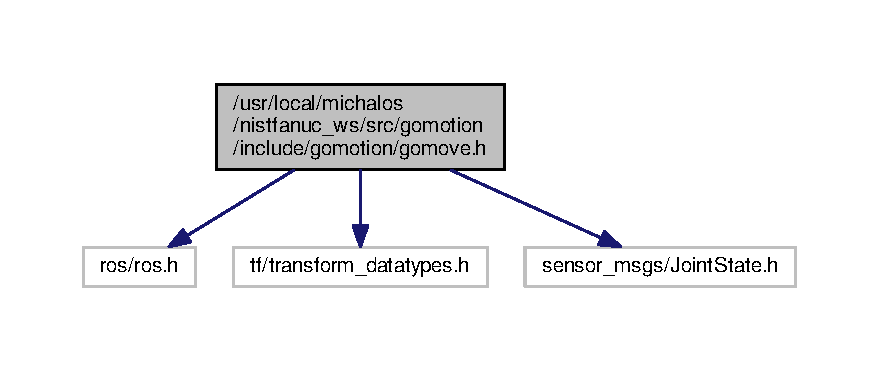
\includegraphics[width=350pt]{db/da4/gomove_8h__incl}
\end{center}
\end{figure}
This graph shows which files directly or indirectly include this file\-:\nopagebreak
\begin{figure}[H]
\begin{center}
\leavevmode
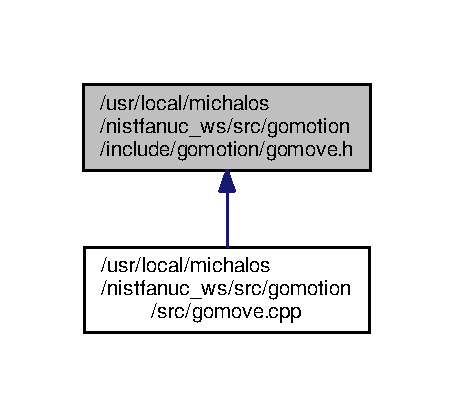
\includegraphics[width=218pt]{de/d43/gomove_8h__dep__incl}
\end{center}
\end{figure}
\subsection*{Data Structures}
\begin{DoxyCompactItemize}
\item 
struct \hyperlink{structgomotion_1_1_go_motion_params}{gomotion\-::\-Go\-Motion\-Params}
\item 
class \hyperlink{classgomotion_1_1_go_motion}{gomotion\-::\-Go\-Motion}
\end{DoxyCompactItemize}
\subsection*{Namespaces}
\begin{DoxyCompactItemize}
\item 
\hyperlink{namespacegomotion}{gomotion}
\end{DoxyCompactItemize}
\subsection*{Typedefs}
\begin{DoxyCompactItemize}
\item 
typedef \\*
sensor\-\_\-msgs\-::\-Joint\-State\-\_\-\\*
$<$ std\-::allocator$<$ void $>$ $>$ \hyperlink{namespacegomotion_a7b9d543e8aa36dfc345c5c38df12d427}{gomotion\-::\-Joint\-State}
\end{DoxyCompactItemize}

\hypertarget{gotraj_8h}{\section{/usr/local/michalos/nistfanuc\-\_\-ws/src/gomotion/include/gomotion/gotraj.h File Reference}
\label{gotraj_8h}\index{/usr/local/michalos/nistfanuc\-\_\-ws/src/gomotion/include/gomotion/gotraj.\-h@{/usr/local/michalos/nistfanuc\-\_\-ws/src/gomotion/include/gomotion/gotraj.\-h}}
}
{\ttfamily \#include $<$math.\-h$>$}\\*
{\ttfamily \#include \char`\"{}gomotion/gotypes.\-h\char`\"{}}\\*
{\ttfamily \#include \char`\"{}gomotion/gomath.\-h\char`\"{}}\\*
Include dependency graph for gotraj.\-h\-:\nopagebreak
\begin{figure}[H]
\begin{center}
\leavevmode
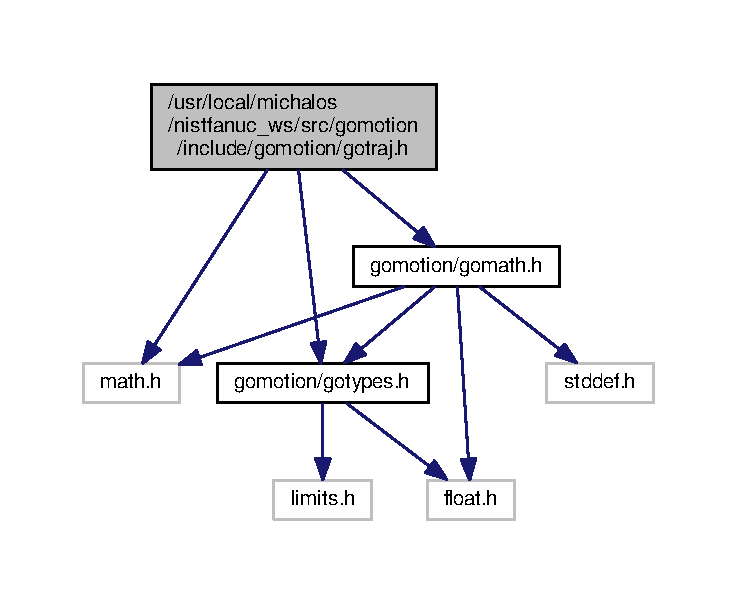
\includegraphics[width=350pt]{d7/d7f/gotraj_8h__incl}
\end{center}
\end{figure}
This graph shows which files directly or indirectly include this file\-:\nopagebreak
\begin{figure}[H]
\begin{center}
\leavevmode
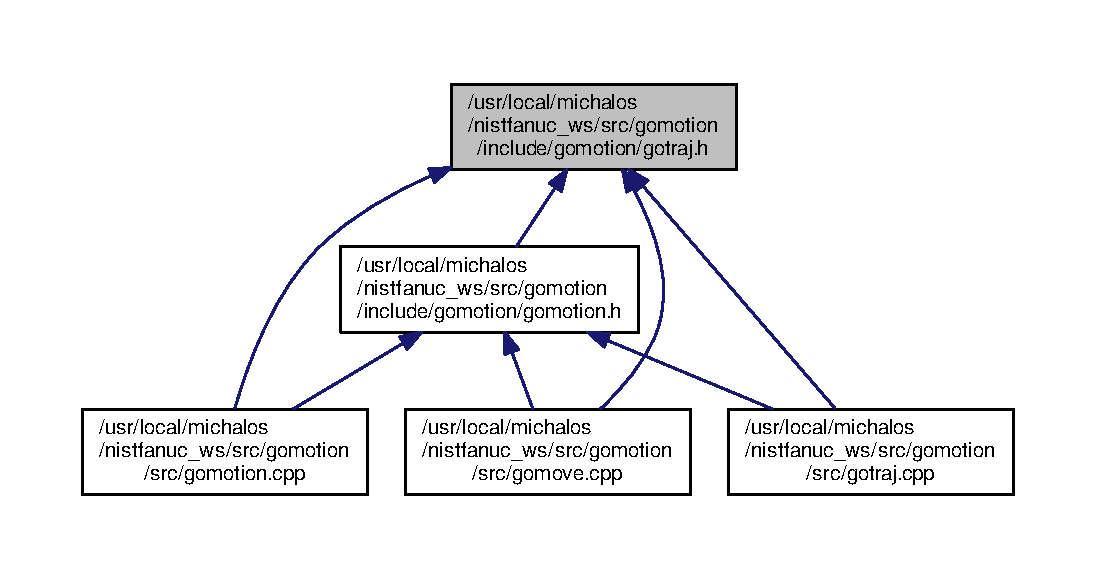
\includegraphics[width=350pt]{d5/d79/gotraj_8h__dep__incl}
\end{center}
\end{figure}
\subsection*{Data Structures}
\begin{DoxyCompactItemize}
\item 
struct \hyperlink{structgomotion_1_1go__traj__ca__spec}{gomotion\-::go\-\_\-traj\-\_\-ca\-\_\-spec}
\item 
struct \hyperlink{structgomotion_1_1go__traj__cj__spec}{gomotion\-::go\-\_\-traj\-\_\-cj\-\_\-spec}
\item 
struct \hyperlink{structgomotion_1_1go__traj__interp__spec}{gomotion\-::go\-\_\-traj\-\_\-interp\-\_\-spec}
\end{DoxyCompactItemize}
\subsection*{Namespaces}
\begin{DoxyCompactItemize}
\item 
\hyperlink{namespacegomotion}{gomotion}
\end{DoxyCompactItemize}
\subsection*{Macros}
\begin{DoxyCompactItemize}
\item 
\#define \hyperlink{gotraj_8h_a89d72de1451dd1598f10db5270b68eea}{reciprocate}(x)~(x) $<$= 0.\-0 ? \hyperlink{gotypes_8h_a1945bf75890ff16eb0d82f5fd231d44e}{G\-O\-\_\-\-I\-N\-F} \-: 1.\-0 / (x)
\end{DoxyCompactItemize}
\subsection*{Functions}
\begin{DoxyCompactItemize}
\item 
\hyperlink{gotypes_8h_a55d48b38cd959f63c7e8db8337a9792a}{go\-\_\-result} \hyperlink{namespacegomotion_ad926ed07425571d1df303c65bc22161f}{gomotion\-::go\-\_\-traj\-\_\-ca\-\_\-generate} (\hyperlink{gotypes_8h_afd666a2393eebd71ee455846ac9def9b}{go\-\_\-real} acc, \hyperlink{gotypes_8h_afd666a2393eebd71ee455846ac9def9b}{go\-\_\-real} deltacc, \hyperlink{gotypes_8h_afd666a2393eebd71ee455846ac9def9b}{go\-\_\-real} deltvel, go\-\_\-traj\-\_\-ca\-\_\-spec $\ast$pts)
\begin{DoxyCompactList}\small\item\em \hyperlink{namespacegomotion_ad926ed07425571d1df303c65bc22161f}{go\-\_\-traj\-\_\-ca\-\_\-generate()} takes an accel value, and intervals for the accel period and cruise period, and fills in the \hyperlink{structgomotion_1_1go__traj__ca__spec}{go\-\_\-traj\-\_\-ca\-\_\-spec} with the interval parameters. \end{DoxyCompactList}\item 
\hyperlink{gotypes_8h_a55d48b38cd959f63c7e8db8337a9792a}{go\-\_\-result} \hyperlink{namespacegomotion_a7c957035ba66766366a69beed80f9193}{gomotion\-::go\-\_\-traj\-\_\-ca\-\_\-compute} (\hyperlink{gotypes_8h_afd666a2393eebd71ee455846ac9def9b}{go\-\_\-real} d, \hyperlink{gotypes_8h_afd666a2393eebd71ee455846ac9def9b}{go\-\_\-real} v, \hyperlink{gotypes_8h_afd666a2393eebd71ee455846ac9def9b}{go\-\_\-real} a, go\-\_\-traj\-\_\-ca\-\_\-spec $\ast$pts)
\begin{DoxyCompactList}\small\item\em \hyperlink{namespacegomotion_a7c957035ba66766366a69beed80f9193}{go\-\_\-traj\-\_\-ca\-\_\-compute()} takes values for distance 'd' to move, max velocity 'v' to limit if necessary, and constant accel 'a', and fills in the \hyperlink{structgomotion_1_1go__traj__ca__spec}{go\-\_\-traj\-\_\-ca\-\_\-spec} with the interval parameters. \end{DoxyCompactList}\item 
\hyperlink{gotypes_8h_a55d48b38cd959f63c7e8db8337a9792a}{go\-\_\-result} \hyperlink{namespacegomotion_a116794cb4157c4f54caf98f65a2ec44f}{gomotion\-::go\-\_\-traj\-\_\-ca\-\_\-scale} (const go\-\_\-traj\-\_\-ca\-\_\-spec $\ast$ts, \hyperlink{gotypes_8h_afd666a2393eebd71ee455846ac9def9b}{go\-\_\-real} t, go\-\_\-traj\-\_\-ca\-\_\-spec $\ast$pts)
\begin{DoxyCompactList}\small\item\em \hyperlink{namespacegomotion_a116794cb4157c4f54caf98f65a2ec44f}{go\-\_\-traj\-\_\-ca\-\_\-scale()} takes a time 't' for the desired time of the motion, and scales the times and motion params so that the total distance remains the same and everything else is in proportion \end{DoxyCompactList}\item 
\hyperlink{gotypes_8h_a55d48b38cd959f63c7e8db8337a9792a}{go\-\_\-result} \hyperlink{namespacegomotion_aeb9f59e687213362972a8405d6210b11}{gomotion\-::go\-\_\-traj\-\_\-ca\-\_\-stop} (const go\-\_\-traj\-\_\-ca\-\_\-spec $\ast$ts, \hyperlink{gotypes_8h_afd666a2393eebd71ee455846ac9def9b}{go\-\_\-real} t, go\-\_\-traj\-\_\-ca\-\_\-spec $\ast$pts)
\begin{DoxyCompactList}\small\item\em \hyperlink{namespacegomotion_aeb9f59e687213362972a8405d6210b11}{go\-\_\-traj\-\_\-ca\-\_\-stop()} takes a time 't' for the desired time to begin stopping, and recomputes the times so that the move will stop as soon as possible during subsequent interps. \end{DoxyCompactList}\item 
\hyperlink{gotypes_8h_a55d48b38cd959f63c7e8db8337a9792a}{go\-\_\-result} \hyperlink{namespacegomotion_a5f1160c8b5662ad14fb8987be62e379d}{gomotion\-::go\-\_\-traj\-\_\-ca\-\_\-extend} (const go\-\_\-traj\-\_\-ca\-\_\-spec $\ast$ts, \hyperlink{gotypes_8h_afd666a2393eebd71ee455846ac9def9b}{go\-\_\-real} t, go\-\_\-traj\-\_\-ca\-\_\-spec $\ast$pts)
\begin{DoxyCompactList}\small\item\em \hyperlink{namespacegomotion_a5f1160c8b5662ad14fb8987be62e379d}{go\-\_\-traj\-\_\-ca\-\_\-extend()} takes a time 't' for the desired time to finish the motion, and extends the constant-\/speed section so that it stops then. \end{DoxyCompactList}\item 
\hyperlink{gotypes_8h_a55d48b38cd959f63c7e8db8337a9792a}{go\-\_\-result} \hyperlink{namespacegomotion_aa138950bb1c02fcbeeb017e61fd061e0}{gomotion\-::go\-\_\-traj\-\_\-ca\-\_\-interp} (const go\-\_\-traj\-\_\-ca\-\_\-spec $\ast$ts, \hyperlink{gotypes_8h_afd666a2393eebd71ee455846ac9def9b}{go\-\_\-real} t, go\-\_\-traj\-\_\-interp\-\_\-spec $\ast$ti)
\begin{DoxyCompactList}\small\item\em \hyperlink{namespacegomotion_aa138950bb1c02fcbeeb017e61fd061e0}{go\-\_\-traj\-\_\-ca\-\_\-interp()} takes a \hyperlink{structgomotion_1_1go__traj__ca__spec}{go\-\_\-traj\-\_\-ca\-\_\-spec} and interpolates the d-\/v-\/a values for the given time t, storing the d-\/v-\/a values in ti. \end{DoxyCompactList}\item 
\hyperlink{gotypes_8h_a55d48b38cd959f63c7e8db8337a9792a}{go\-\_\-result} \hyperlink{namespacegomotion_a6e56fd184b0ec5ce1668553a315c0ed7}{gomotion\-::go\-\_\-traj\-\_\-cj\-\_\-generate} (\hyperlink{gotypes_8h_afd666a2393eebd71ee455846ac9def9b}{go\-\_\-real} jrk, \hyperlink{gotypes_8h_afd666a2393eebd71ee455846ac9def9b}{go\-\_\-real} deltjrk, \hyperlink{gotypes_8h_afd666a2393eebd71ee455846ac9def9b}{go\-\_\-real} deltacc, \hyperlink{gotypes_8h_afd666a2393eebd71ee455846ac9def9b}{go\-\_\-real} deltvel, go\-\_\-traj\-\_\-cj\-\_\-spec $\ast$pts)
\begin{DoxyCompactList}\small\item\em \hyperlink{namespacegomotion_a6e56fd184b0ec5ce1668553a315c0ed7}{go\-\_\-traj\-\_\-cj\-\_\-generate()} takes a jerk value, and intervals for the jerk period, accel period and cruise period, and fills in the \hyperlink{structgomotion_1_1go__traj__cj__spec}{go\-\_\-traj\-\_\-cj\-\_\-spec} with the interval parameters. \end{DoxyCompactList}\item 
\hyperlink{gotypes_8h_a55d48b38cd959f63c7e8db8337a9792a}{go\-\_\-result} \hyperlink{namespacegomotion_a5edc6aa7aad4817534ac8099a2638610}{gomotion\-::go\-\_\-traj\-\_\-cj\-\_\-compute} (\hyperlink{gotypes_8h_afd666a2393eebd71ee455846ac9def9b}{go\-\_\-real} d, \hyperlink{gotypes_8h_afd666a2393eebd71ee455846ac9def9b}{go\-\_\-real} v, \hyperlink{gotypes_8h_afd666a2393eebd71ee455846ac9def9b}{go\-\_\-real} a, \hyperlink{gotypes_8h_afd666a2393eebd71ee455846ac9def9b}{go\-\_\-real} j, go\-\_\-traj\-\_\-cj\-\_\-spec $\ast$pts)
\begin{DoxyCompactList}\small\item\em \hyperlink{namespacegomotion_a5edc6aa7aad4817534ac8099a2638610}{go\-\_\-traj\-\_\-cj\-\_\-compute()} takes values for distance 'd' to move, max velocity 'v' to limit if necessary, max accel 'a' to limit if necessary, and constant jerk 'j', and fills in the \hyperlink{structgomotion_1_1go__traj__cj__spec}{go\-\_\-traj\-\_\-cj\-\_\-spec} with the interval parameters. \end{DoxyCompactList}\item 
\hyperlink{gotypes_8h_a55d48b38cd959f63c7e8db8337a9792a}{go\-\_\-result} \hyperlink{namespacegomotion_a6597fcefe873523be5a8a7a587788b53}{gomotion\-::go\-\_\-traj\-\_\-cj\-\_\-scale} (const go\-\_\-traj\-\_\-cj\-\_\-spec $\ast$ts, \hyperlink{gotypes_8h_afd666a2393eebd71ee455846ac9def9b}{go\-\_\-real} t, go\-\_\-traj\-\_\-cj\-\_\-spec $\ast$pts)
\begin{DoxyCompactList}\small\item\em \hyperlink{namespacegomotion_a6597fcefe873523be5a8a7a587788b53}{go\-\_\-traj\-\_\-cj\-\_\-scale()} takes a time 't' for the desired time of the motion, and scales the times and motion params so that the total distance remains the same and everything else is in proportion \end{DoxyCompactList}\item 
\hyperlink{gotypes_8h_a55d48b38cd959f63c7e8db8337a9792a}{go\-\_\-result} \hyperlink{namespacegomotion_a0764efa1b4a4385aaf9fe13e0ea7b812}{gomotion\-::go\-\_\-traj\-\_\-cj\-\_\-stop} (const go\-\_\-traj\-\_\-cj\-\_\-spec $\ast$ts, \hyperlink{gotypes_8h_afd666a2393eebd71ee455846ac9def9b}{go\-\_\-real} t, go\-\_\-traj\-\_\-cj\-\_\-spec $\ast$pts)
\begin{DoxyCompactList}\small\item\em \hyperlink{namespacegomotion_a0764efa1b4a4385aaf9fe13e0ea7b812}{go\-\_\-traj\-\_\-cj\-\_\-stop()} takes a time 't' for the desired time to begin stopping, and recomputes the times so that the move will stop as soon as possible during subsequent interps. \end{DoxyCompactList}\item 
\hyperlink{gotypes_8h_a55d48b38cd959f63c7e8db8337a9792a}{go\-\_\-result} \hyperlink{namespacegomotion_ad6229b01a04c2232c7535f600849bb73}{gomotion\-::go\-\_\-traj\-\_\-cj\-\_\-extend} (const go\-\_\-traj\-\_\-cj\-\_\-spec $\ast$ts, \hyperlink{gotypes_8h_afd666a2393eebd71ee455846ac9def9b}{go\-\_\-real} t, go\-\_\-traj\-\_\-cj\-\_\-spec $\ast$pts)
\begin{DoxyCompactList}\small\item\em \hyperlink{namespacegomotion_ad6229b01a04c2232c7535f600849bb73}{go\-\_\-traj\-\_\-cj\-\_\-extend()} takes a time 't' for the desired time to finish the motion, and extends the constant-\/speed section so that it stops then. \end{DoxyCompactList}\item 
\hyperlink{gotypes_8h_a55d48b38cd959f63c7e8db8337a9792a}{go\-\_\-result} \hyperlink{namespacegomotion_a2d66e2943e92ad2df63ae5d008eb8a6c}{gomotion\-::go\-\_\-traj\-\_\-cj\-\_\-interp} (const go\-\_\-traj\-\_\-cj\-\_\-spec $\ast$ts, \hyperlink{gotypes_8h_afd666a2393eebd71ee455846ac9def9b}{go\-\_\-real} t, go\-\_\-traj\-\_\-interp\-\_\-spec $\ast$ti)
\begin{DoxyCompactList}\small\item\em \hyperlink{namespacegomotion_a2d66e2943e92ad2df63ae5d008eb8a6c}{go\-\_\-traj\-\_\-cj\-\_\-interp()} takes a \hyperlink{structgomotion_1_1go__traj__cj__spec}{go\-\_\-traj\-\_\-cj\-\_\-spec} and interpolates the d-\/v-\/a-\/j values for the given time t, storing the d-\/v-\/a-\/j values in ti. \end{DoxyCompactList}\item 
\hyperlink{gotypes_8h_a55d48b38cd959f63c7e8db8337a9792a}{go\-\_\-result} \hyperlink{namespacegomotion_a396781d83275b54de406e65a5c944093}{gomotion\-::go\-\_\-traj\-\_\-cj\-\_\-compute\-\_\-the\-\_\-rest} (go\-\_\-traj\-\_\-cj\-\_\-spec $\ast$pts)
\begin{DoxyCompactList}\small\item\em ! Expects {\itshape pts} attributes {\itshape dtend}, {\itshape jt0}, {\itshape at1}, {\itshape vt3}, {\itshape t1}, {\itshape t2} and {\itshape t3} to be already filled in from previous calls to one of the four {\itshape go\-\_\-traj\-\_\-cj\-\_\-compute\-\_\-tees} functions and {\itshape go\-\_\-traj\-\_\-cj\-\_\-compute}. \end{DoxyCompactList}\item 
\hyperlink{gotypes_8h_a55d48b38cd959f63c7e8db8337a9792a}{go\-\_\-result} \hyperlink{namespacegomotion_a9cabcec05e99b4da69912b42fcc637e5}{gomotion\-::go\-\_\-traj\-\_\-cj\-\_\-compute\-\_\-tees\-\_\-na\-\_\-nc} (go\-\_\-traj\-\_\-cj\-\_\-spec $\ast$pts)
\begin{DoxyCompactList}\small\item\em ! Computes the trajectory defining times {\itshape t1}, {\itshape t2} and {\itshape t4} for a motion with no acceleration or cruise phase, given {\itshape pts} filled in with {\itshape dtend} and {\itshape jt0}. \end{DoxyCompactList}\item 
\hyperlink{gotypes_8h_a55d48b38cd959f63c7e8db8337a9792a}{go\-\_\-result} \hyperlink{namespacegomotion_af869a1a311f90bfd85c552a5a5fed4a1}{gomotion\-::go\-\_\-traj\-\_\-cj\-\_\-compute\-\_\-tees\-\_\-a\-\_\-nc} (go\-\_\-traj\-\_\-cj\-\_\-spec $\ast$pts)
\begin{DoxyCompactList}\small\item\em ! Computes the trajectory defining times {\itshape t1}, {\itshape t2} and {\itshape t4} for a motion with acceleration but no cruise phase, given {\itshape pts} filled in with {\itshape dtend}, {\itshape jt0} and {\itshape at1}. \end{DoxyCompactList}\item 
\hyperlink{gotypes_8h_a55d48b38cd959f63c7e8db8337a9792a}{go\-\_\-result} \hyperlink{namespacegomotion_ac06c11fdcb4ac07e6bd860c904644c52}{gomotion\-::go\-\_\-traj\-\_\-cj\-\_\-compute\-\_\-tees\-\_\-na\-\_\-c} (go\-\_\-traj\-\_\-cj\-\_\-spec $\ast$pts)
\begin{DoxyCompactList}\small\item\em ! Computes the trajectory defining times {\itshape t1}, {\itshape t2} and {\itshape t4} for a motion with no acceleration but a cruise phase, given {\itshape pts} filled in with {\itshape dtend}, {\itshape jt0} and {\itshape vt3}. \end{DoxyCompactList}\item 
\hyperlink{gotypes_8h_a55d48b38cd959f63c7e8db8337a9792a}{go\-\_\-result} \hyperlink{namespacegomotion_a474f6e7cd5710ecb20c7fe42d188ddc9}{gomotion\-::go\-\_\-traj\-\_\-cj\-\_\-compute\-\_\-tees\-\_\-a\-\_\-c} (go\-\_\-traj\-\_\-cj\-\_\-spec $\ast$pts)
\begin{DoxyCompactList}\small\item\em ! Computes the trajectory defining times {\itshape t1}, {\itshape t2} and {\itshape t4} for a motion with no acceleration but a cruise phase, given {\itshape pts} filled in with {\itshape dtend}, {\itshape jt0}, at1 and {\itshape vt3}. \end{DoxyCompactList}\end{DoxyCompactItemize}


\subsection{Macro Definition Documentation}
\hypertarget{gotraj_8h_a89d72de1451dd1598f10db5270b68eea}{\index{gotraj.\-h@{gotraj.\-h}!reciprocate@{reciprocate}}
\index{reciprocate@{reciprocate}!gotraj.h@{gotraj.\-h}}
\subsubsection[{reciprocate}]{\setlength{\rightskip}{0pt plus 5cm}\#define reciprocate(
\begin{DoxyParamCaption}
\item[{}]{x}
\end{DoxyParamCaption}
)~(x) $<$= 0.\-0 ? {\bf G\-O\-\_\-\-I\-N\-F} \-: 1.\-0 / (x)}}\label{gotraj_8h_a89d72de1451dd1598f10db5270b68eea}

\hypertarget{gotypes_8h}{\section{/usr/local/michalos/nistfanuc\-\_\-ws/src/gomotion/include/gomotion/gotypes.h File Reference}
\label{gotypes_8h}\index{/usr/local/michalos/nistfanuc\-\_\-ws/src/gomotion/include/gomotion/gotypes.\-h@{/usr/local/michalos/nistfanuc\-\_\-ws/src/gomotion/include/gomotion/gotypes.\-h}}
}
{\ttfamily \#include $<$float.\-h$>$}\\*
{\ttfamily \#include $<$limits.\-h$>$}\\*
Include dependency graph for gotypes.\-h\-:\nopagebreak
\begin{figure}[H]
\begin{center}
\leavevmode
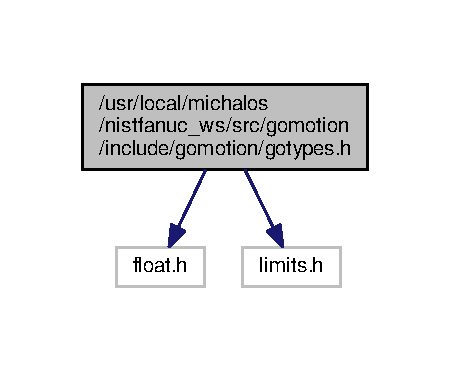
\includegraphics[width=216pt]{d2/d4b/gotypes_8h__incl}
\end{center}
\end{figure}
This graph shows which files directly or indirectly include this file\-:\nopagebreak
\begin{figure}[H]
\begin{center}
\leavevmode
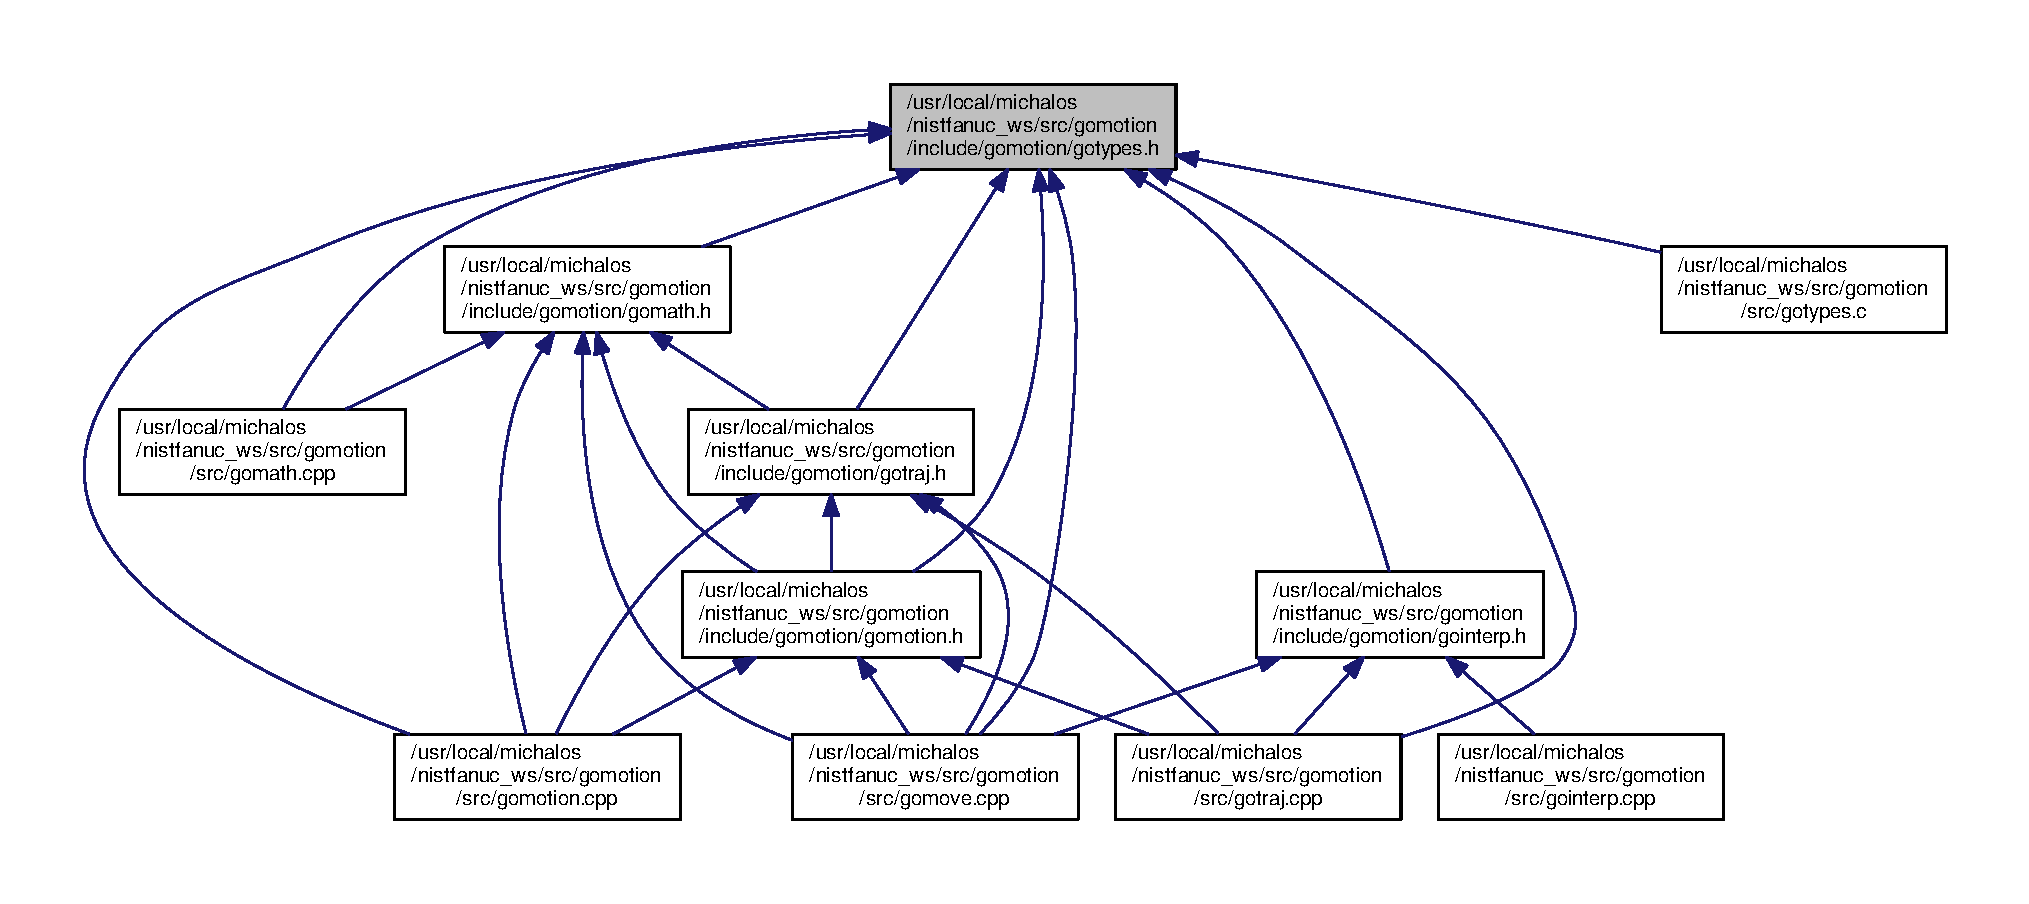
\includegraphics[width=350pt]{de/d16/gotypes_8h__dep__incl}
\end{center}
\end{figure}
\subsection*{Macros}
\begin{DoxyCompactItemize}
\item 
\#define \hyperlink{gotypes_8h_acdff3c13e07e2c52b319862205a69a7b}{G\-O\-\_\-\-R\-E\-S\-U\-L\-T\-\_\-\-I\-N\-T}
\item 
\#define \hyperlink{gotypes_8h_a0a6c11884a321b4068131799a75cc8d3}{G\-O\-\_\-\-R\-E\-S\-U\-L\-T}~\hyperlink{gotypes_8h_a184d14380dbe5f6c91a5038cea6ea6f5}{go\-\_\-result\-\_\-int}
\item 
\#define \hyperlink{gotypes_8h_a8eb31e96aaba893c1af95b3504a72c9e}{go\-\_\-result\-\_\-to\-\_\-string}(r)
\item 
\#define \hyperlink{gotypes_8h_a2e8a5593d6ac2fe05853e89a35c34e40}{go\-\_\-quantity\-\_\-to\-\_\-string}(q)
\item 
\#define \hyperlink{gotypes_8h_a47189b2c0645196d6b9fb1371cfce1b5}{G\-O\-\_\-\-R\-E\-A\-L\-\_\-\-D\-O\-U\-B\-L\-E}
\item 
\#define \hyperlink{gotypes_8h_a285b45e695b1b820ddbb5306354fcf94}{G\-O\-\_\-\-R\-E\-A\-L}~\hyperlink{gotypes_8h_ac774d0767586d2cfcc72c5a8b2e063a0}{go\-\_\-real\-\_\-double}
\item 
\#define \hyperlink{gotypes_8h_a5effba89a60b0bcc04dcd5c2c917adce}{G\-O\-\_\-\-R\-E\-A\-L\-\_\-\-M\-I\-N}~D\-B\-L\-\_\-\-M\-I\-N
\item 
\#define \hyperlink{gotypes_8h_aa9b9ea9d84a3616fd7bf5ca8f0518e54}{G\-O\-\_\-\-R\-E\-A\-L\-\_\-\-M\-A\-X}~D\-B\-L\-\_\-\-M\-A\-X
\item 
\#define \hyperlink{gotypes_8h_a565feef8b688896bae12bba085027170}{G\-O\-\_\-\-R\-E\-A\-L\-\_\-\-E\-P\-S\-I\-L\-O\-N}~(1.\-0e-\/7)
\item 
\#define \hyperlink{gotypes_8h_a1945bf75890ff16eb0d82f5fd231d44e}{G\-O\-\_\-\-I\-N\-F}~D\-B\-L\-\_\-\-M\-A\-X
\item 
\#define \hyperlink{gotypes_8h_ae5a9c4fcfa17cd2046debe6a7eb1bcd5}{G\-O\-\_\-\-I\-N\-T\-E\-G\-E\-R\-\_\-\-I\-N\-T}
\item 
\#define \hyperlink{gotypes_8h_af3a59e902c2952ed05fb79c7e8850ef6}{G\-O\-\_\-\-I\-N\-T\-E\-G\-E\-R}~\hyperlink{gotypes_8h_a35b4eb7b07fa8a2c89a4ff5e77a61ca3}{go\-\_\-integer\-\_\-int}
\item 
\#define \hyperlink{gotypes_8h_a551785048d56fd51202f0b79508fbb4d}{G\-O\-\_\-\-I\-N\-T\-E\-G\-E\-R\-\_\-\-M\-A\-X}~I\-N\-T\-\_\-\-M\-A\-X
\item 
\#define \hyperlink{gotypes_8h_abebbcdc81fe161ade1ebf57fd7e75080}{G\-O\-\_\-\-F\-L\-A\-G\-\_\-\-U\-C\-H\-A\-R}
\item 
\#define \hyperlink{gotypes_8h_a08cfa9bb505541a7554cabb1281bf27e}{G\-O\-\_\-\-F\-L\-A\-G}~\hyperlink{gotypes_8h_a5b26be2f7a574d308ae9cbc14c7a8fac}{go\-\_\-flag\-\_\-uchar}
\end{DoxyCompactItemize}
\subsection*{Typedefs}
\begin{DoxyCompactItemize}
\item 
typedef int \hyperlink{gotypes_8h_a55d48b38cd959f63c7e8db8337a9792a}{go\-\_\-result}
\item 
typedef double \hyperlink{gotypes_8h_afd666a2393eebd71ee455846ac9def9b}{go\-\_\-real}
\item 
typedef int \hyperlink{gotypes_8h_a7d30f606bb0f58ffe2b3bd71e5c8af5c}{go\-\_\-integer}
\item 
typedef unsigned char \hyperlink{gotypes_8h_ae890d9a0ddecc0d3073622cc4312092d}{go\-\_\-flag}
\end{DoxyCompactItemize}
\subsection*{Enumerations}
\begin{DoxyCompactItemize}
\item 
enum \{ \\*
\hyperlink{gotypes_8h_a726ca809ffd3d67ab4b8476646f26635a474a770c6dd01e6ff6d9316bec185bdc}{G\-O\-\_\-\-R\-E\-S\-U\-L\-T\-\_\-\-O\-K} = 0, 
\hyperlink{gotypes_8h_a726ca809ffd3d67ab4b8476646f26635a2ce6982cf7db77b01c9757c92b8850ac}{G\-O\-\_\-\-R\-E\-S\-U\-L\-T\-\_\-\-I\-G\-N\-O\-R\-E\-D}, 
\hyperlink{gotypes_8h_a726ca809ffd3d67ab4b8476646f26635a774dfa8abb1bab8ff8599bbcacefa13e}{G\-O\-\_\-\-R\-E\-S\-U\-L\-T\-\_\-\-B\-A\-D\-\_\-\-A\-R\-G\-S}, 
\hyperlink{gotypes_8h_a726ca809ffd3d67ab4b8476646f26635adbdc03b02695760e5650a9c03dba3d0e}{G\-O\-\_\-\-R\-E\-S\-U\-L\-T\-\_\-\-R\-A\-N\-G\-E\-\_\-\-E\-R\-R\-O\-R}, 
\\*
\hyperlink{gotypes_8h_a726ca809ffd3d67ab4b8476646f26635a59be6a201b1e7b8905a0c89eec00963b}{G\-O\-\_\-\-R\-E\-S\-U\-L\-T\-\_\-\-D\-O\-M\-A\-I\-N\-\_\-\-E\-R\-R\-O\-R}, 
\hyperlink{gotypes_8h_a726ca809ffd3d67ab4b8476646f26635acbf54540acb86538b3f72b4b8e0a176d}{G\-O\-\_\-\-R\-E\-S\-U\-L\-T\-\_\-\-E\-R\-R\-O\-R}, 
\hyperlink{gotypes_8h_a726ca809ffd3d67ab4b8476646f26635a9d6bb28a1830d96c3dc0c0154153d80a}{G\-O\-\_\-\-R\-E\-S\-U\-L\-T\-\_\-\-I\-M\-P\-L\-\_\-\-E\-R\-R\-O\-R}, 
\hyperlink{gotypes_8h_a726ca809ffd3d67ab4b8476646f26635a03cf3256a6fc44ee40192ed232d4c659}{G\-O\-\_\-\-R\-E\-S\-U\-L\-T\-\_\-\-N\-O\-R\-M\-\_\-\-E\-R\-R\-O\-R}, 
\\*
\hyperlink{gotypes_8h_a726ca809ffd3d67ab4b8476646f26635ac2434e23b7ae651aebe2452af7af1995}{G\-O\-\_\-\-R\-E\-S\-U\-L\-T\-\_\-\-D\-I\-V\-\_\-\-E\-R\-R\-O\-R}, 
\hyperlink{gotypes_8h_a726ca809ffd3d67ab4b8476646f26635a0f2b551fe19dd46697296b56b83ef1d7}{G\-O\-\_\-\-R\-E\-S\-U\-L\-T\-\_\-\-S\-I\-N\-G\-U\-L\-A\-R}, 
\hyperlink{gotypes_8h_a726ca809ffd3d67ab4b8476646f26635ad1cc08529bcdd199480d3d57e53b5d84}{G\-O\-\_\-\-R\-E\-S\-U\-L\-T\-\_\-\-N\-O\-\_\-\-S\-P\-A\-C\-E}, 
\hyperlink{gotypes_8h_a726ca809ffd3d67ab4b8476646f26635a24838323a80d8fd8a140c92473f740e3}{G\-O\-\_\-\-R\-E\-S\-U\-L\-T\-\_\-\-E\-M\-P\-T\-Y}, 
\\*
\hyperlink{gotypes_8h_a726ca809ffd3d67ab4b8476646f26635a5524763e925f0b14dcba6a321574bba7}{G\-O\-\_\-\-R\-E\-S\-U\-L\-T\-\_\-\-B\-U\-G}
 \}
\item 
enum \{ \hyperlink{gotypes_8h_a0411cd49bb5b71852cecd93bcbf0ca2daaf19b8b96ec24aee3e4bc35efc855a24}{G\-O\-\_\-\-Q\-U\-A\-N\-T\-I\-T\-Y\-\_\-\-N\-O\-N\-E} = 0, 
\hyperlink{gotypes_8h_a0411cd49bb5b71852cecd93bcbf0ca2da847a795c80c454fb18dd2843b9a5ae37}{G\-O\-\_\-\-Q\-U\-A\-N\-T\-I\-T\-Y\-\_\-\-L\-E\-N\-G\-T\-H}, 
\hyperlink{gotypes_8h_a0411cd49bb5b71852cecd93bcbf0ca2da70505768da54108916ca9d850a345c16}{G\-O\-\_\-\-Q\-U\-A\-N\-T\-I\-T\-Y\-\_\-\-A\-N\-G\-L\-E}
 \}
\end{DoxyCompactItemize}
\subsection*{Variables}
\begin{DoxyCompactItemize}
\item 
int \hyperlink{gotypes_8h_a184d14380dbe5f6c91a5038cea6ea6f5}{go\-\_\-result\-\_\-int}
\item 
int \hyperlink{gotypes_8h_ac774d0767586d2cfcc72c5a8b2e063a0}{go\-\_\-real\-\_\-double}
\item 
int \hyperlink{gotypes_8h_a35b4eb7b07fa8a2c89a4ff5e77a61ca3}{go\-\_\-integer\-\_\-int}
\item 
int \hyperlink{gotypes_8h_a5b26be2f7a574d308ae9cbc14c7a8fac}{go\-\_\-flag\-\_\-uchar}
\item 
\hyperlink{gotypes_8h_ae890d9a0ddecc0d3073622cc4312092d}{go\-\_\-flag} \hyperlink{gotypes_8h_abb9b839befebbde059804073bd17efd4}{gocode}
\end{DoxyCompactItemize}


\subsection{Macro Definition Documentation}
\hypertarget{gotypes_8h_a08cfa9bb505541a7554cabb1281bf27e}{\index{gotypes.\-h@{gotypes.\-h}!G\-O\-\_\-\-F\-L\-A\-G@{G\-O\-\_\-\-F\-L\-A\-G}}
\index{G\-O\-\_\-\-F\-L\-A\-G@{G\-O\-\_\-\-F\-L\-A\-G}!gotypes.h@{gotypes.\-h}}
\subsubsection[{G\-O\-\_\-\-F\-L\-A\-G}]{\setlength{\rightskip}{0pt plus 5cm}\#define G\-O\-\_\-\-F\-L\-A\-G~{\bf go\-\_\-flag\-\_\-uchar}}}\label{gotypes_8h_a08cfa9bb505541a7554cabb1281bf27e}
\hypertarget{gotypes_8h_abebbcdc81fe161ade1ebf57fd7e75080}{\index{gotypes.\-h@{gotypes.\-h}!G\-O\-\_\-\-F\-L\-A\-G\-\_\-\-U\-C\-H\-A\-R@{G\-O\-\_\-\-F\-L\-A\-G\-\_\-\-U\-C\-H\-A\-R}}
\index{G\-O\-\_\-\-F\-L\-A\-G\-\_\-\-U\-C\-H\-A\-R@{G\-O\-\_\-\-F\-L\-A\-G\-\_\-\-U\-C\-H\-A\-R}!gotypes.h@{gotypes.\-h}}
\subsubsection[{G\-O\-\_\-\-F\-L\-A\-G\-\_\-\-U\-C\-H\-A\-R}]{\setlength{\rightskip}{0pt plus 5cm}\#define G\-O\-\_\-\-F\-L\-A\-G\-\_\-\-U\-C\-H\-A\-R}}\label{gotypes_8h_abebbcdc81fe161ade1ebf57fd7e75080}
\hypertarget{gotypes_8h_a1945bf75890ff16eb0d82f5fd231d44e}{\index{gotypes.\-h@{gotypes.\-h}!G\-O\-\_\-\-I\-N\-F@{G\-O\-\_\-\-I\-N\-F}}
\index{G\-O\-\_\-\-I\-N\-F@{G\-O\-\_\-\-I\-N\-F}!gotypes.h@{gotypes.\-h}}
\subsubsection[{G\-O\-\_\-\-I\-N\-F}]{\setlength{\rightskip}{0pt plus 5cm}\#define G\-O\-\_\-\-I\-N\-F~D\-B\-L\-\_\-\-M\-A\-X}}\label{gotypes_8h_a1945bf75890ff16eb0d82f5fd231d44e}
\hypertarget{gotypes_8h_af3a59e902c2952ed05fb79c7e8850ef6}{\index{gotypes.\-h@{gotypes.\-h}!G\-O\-\_\-\-I\-N\-T\-E\-G\-E\-R@{G\-O\-\_\-\-I\-N\-T\-E\-G\-E\-R}}
\index{G\-O\-\_\-\-I\-N\-T\-E\-G\-E\-R@{G\-O\-\_\-\-I\-N\-T\-E\-G\-E\-R}!gotypes.h@{gotypes.\-h}}
\subsubsection[{G\-O\-\_\-\-I\-N\-T\-E\-G\-E\-R}]{\setlength{\rightskip}{0pt plus 5cm}\#define G\-O\-\_\-\-I\-N\-T\-E\-G\-E\-R~{\bf go\-\_\-integer\-\_\-int}}}\label{gotypes_8h_af3a59e902c2952ed05fb79c7e8850ef6}
\hypertarget{gotypes_8h_ae5a9c4fcfa17cd2046debe6a7eb1bcd5}{\index{gotypes.\-h@{gotypes.\-h}!G\-O\-\_\-\-I\-N\-T\-E\-G\-E\-R\-\_\-\-I\-N\-T@{G\-O\-\_\-\-I\-N\-T\-E\-G\-E\-R\-\_\-\-I\-N\-T}}
\index{G\-O\-\_\-\-I\-N\-T\-E\-G\-E\-R\-\_\-\-I\-N\-T@{G\-O\-\_\-\-I\-N\-T\-E\-G\-E\-R\-\_\-\-I\-N\-T}!gotypes.h@{gotypes.\-h}}
\subsubsection[{G\-O\-\_\-\-I\-N\-T\-E\-G\-E\-R\-\_\-\-I\-N\-T}]{\setlength{\rightskip}{0pt plus 5cm}\#define G\-O\-\_\-\-I\-N\-T\-E\-G\-E\-R\-\_\-\-I\-N\-T}}\label{gotypes_8h_ae5a9c4fcfa17cd2046debe6a7eb1bcd5}
\hypertarget{gotypes_8h_a551785048d56fd51202f0b79508fbb4d}{\index{gotypes.\-h@{gotypes.\-h}!G\-O\-\_\-\-I\-N\-T\-E\-G\-E\-R\-\_\-\-M\-A\-X@{G\-O\-\_\-\-I\-N\-T\-E\-G\-E\-R\-\_\-\-M\-A\-X}}
\index{G\-O\-\_\-\-I\-N\-T\-E\-G\-E\-R\-\_\-\-M\-A\-X@{G\-O\-\_\-\-I\-N\-T\-E\-G\-E\-R\-\_\-\-M\-A\-X}!gotypes.h@{gotypes.\-h}}
\subsubsection[{G\-O\-\_\-\-I\-N\-T\-E\-G\-E\-R\-\_\-\-M\-A\-X}]{\setlength{\rightskip}{0pt plus 5cm}\#define G\-O\-\_\-\-I\-N\-T\-E\-G\-E\-R\-\_\-\-M\-A\-X~I\-N\-T\-\_\-\-M\-A\-X}}\label{gotypes_8h_a551785048d56fd51202f0b79508fbb4d}
\hypertarget{gotypes_8h_a2e8a5593d6ac2fe05853e89a35c34e40}{\index{gotypes.\-h@{gotypes.\-h}!go\-\_\-quantity\-\_\-to\-\_\-string@{go\-\_\-quantity\-\_\-to\-\_\-string}}
\index{go\-\_\-quantity\-\_\-to\-\_\-string@{go\-\_\-quantity\-\_\-to\-\_\-string}!gotypes.h@{gotypes.\-h}}
\subsubsection[{go\-\_\-quantity\-\_\-to\-\_\-string}]{\setlength{\rightskip}{0pt plus 5cm}\#define go\-\_\-quantity\-\_\-to\-\_\-string(
\begin{DoxyParamCaption}
\item[{}]{q}
\end{DoxyParamCaption}
)}}\label{gotypes_8h_a2e8a5593d6ac2fe05853e89a35c34e40}
{\bfseries Value\-:}
\begin{DoxyCode}
(q) == \hyperlink{gotypes_8h_a0411cd49bb5b71852cecd93bcbf0ca2da847a795c80c454fb18dd2843b9a5ae37}{GO\_QUANTITY\_LENGTH} ? \textcolor{stringliteral}{"Length"} :                \(\backslash\)
(q) == \hyperlink{gotypes_8h_a0411cd49bb5b71852cecd93bcbf0ca2da70505768da54108916ca9d850a345c16}{GO\_QUANTITY\_ANGLE} ? \textcolor{stringliteral}{"Angle"} : \textcolor{stringliteral}{"None"}
\end{DoxyCode}
\hypertarget{gotypes_8h_a285b45e695b1b820ddbb5306354fcf94}{\index{gotypes.\-h@{gotypes.\-h}!G\-O\-\_\-\-R\-E\-A\-L@{G\-O\-\_\-\-R\-E\-A\-L}}
\index{G\-O\-\_\-\-R\-E\-A\-L@{G\-O\-\_\-\-R\-E\-A\-L}!gotypes.h@{gotypes.\-h}}
\subsubsection[{G\-O\-\_\-\-R\-E\-A\-L}]{\setlength{\rightskip}{0pt plus 5cm}\#define G\-O\-\_\-\-R\-E\-A\-L~{\bf go\-\_\-real\-\_\-double}}}\label{gotypes_8h_a285b45e695b1b820ddbb5306354fcf94}
\hypertarget{gotypes_8h_a47189b2c0645196d6b9fb1371cfce1b5}{\index{gotypes.\-h@{gotypes.\-h}!G\-O\-\_\-\-R\-E\-A\-L\-\_\-\-D\-O\-U\-B\-L\-E@{G\-O\-\_\-\-R\-E\-A\-L\-\_\-\-D\-O\-U\-B\-L\-E}}
\index{G\-O\-\_\-\-R\-E\-A\-L\-\_\-\-D\-O\-U\-B\-L\-E@{G\-O\-\_\-\-R\-E\-A\-L\-\_\-\-D\-O\-U\-B\-L\-E}!gotypes.h@{gotypes.\-h}}
\subsubsection[{G\-O\-\_\-\-R\-E\-A\-L\-\_\-\-D\-O\-U\-B\-L\-E}]{\setlength{\rightskip}{0pt plus 5cm}\#define G\-O\-\_\-\-R\-E\-A\-L\-\_\-\-D\-O\-U\-B\-L\-E}}\label{gotypes_8h_a47189b2c0645196d6b9fb1371cfce1b5}
\hypertarget{gotypes_8h_a565feef8b688896bae12bba085027170}{\index{gotypes.\-h@{gotypes.\-h}!G\-O\-\_\-\-R\-E\-A\-L\-\_\-\-E\-P\-S\-I\-L\-O\-N@{G\-O\-\_\-\-R\-E\-A\-L\-\_\-\-E\-P\-S\-I\-L\-O\-N}}
\index{G\-O\-\_\-\-R\-E\-A\-L\-\_\-\-E\-P\-S\-I\-L\-O\-N@{G\-O\-\_\-\-R\-E\-A\-L\-\_\-\-E\-P\-S\-I\-L\-O\-N}!gotypes.h@{gotypes.\-h}}
\subsubsection[{G\-O\-\_\-\-R\-E\-A\-L\-\_\-\-E\-P\-S\-I\-L\-O\-N}]{\setlength{\rightskip}{0pt plus 5cm}\#define G\-O\-\_\-\-R\-E\-A\-L\-\_\-\-E\-P\-S\-I\-L\-O\-N~(1.\-0e-\/7)}}\label{gotypes_8h_a565feef8b688896bae12bba085027170}
\hypertarget{gotypes_8h_aa9b9ea9d84a3616fd7bf5ca8f0518e54}{\index{gotypes.\-h@{gotypes.\-h}!G\-O\-\_\-\-R\-E\-A\-L\-\_\-\-M\-A\-X@{G\-O\-\_\-\-R\-E\-A\-L\-\_\-\-M\-A\-X}}
\index{G\-O\-\_\-\-R\-E\-A\-L\-\_\-\-M\-A\-X@{G\-O\-\_\-\-R\-E\-A\-L\-\_\-\-M\-A\-X}!gotypes.h@{gotypes.\-h}}
\subsubsection[{G\-O\-\_\-\-R\-E\-A\-L\-\_\-\-M\-A\-X}]{\setlength{\rightskip}{0pt plus 5cm}\#define G\-O\-\_\-\-R\-E\-A\-L\-\_\-\-M\-A\-X~D\-B\-L\-\_\-\-M\-A\-X}}\label{gotypes_8h_aa9b9ea9d84a3616fd7bf5ca8f0518e54}
\hypertarget{gotypes_8h_a5effba89a60b0bcc04dcd5c2c917adce}{\index{gotypes.\-h@{gotypes.\-h}!G\-O\-\_\-\-R\-E\-A\-L\-\_\-\-M\-I\-N@{G\-O\-\_\-\-R\-E\-A\-L\-\_\-\-M\-I\-N}}
\index{G\-O\-\_\-\-R\-E\-A\-L\-\_\-\-M\-I\-N@{G\-O\-\_\-\-R\-E\-A\-L\-\_\-\-M\-I\-N}!gotypes.h@{gotypes.\-h}}
\subsubsection[{G\-O\-\_\-\-R\-E\-A\-L\-\_\-\-M\-I\-N}]{\setlength{\rightskip}{0pt plus 5cm}\#define G\-O\-\_\-\-R\-E\-A\-L\-\_\-\-M\-I\-N~D\-B\-L\-\_\-\-M\-I\-N}}\label{gotypes_8h_a5effba89a60b0bcc04dcd5c2c917adce}
\hypertarget{gotypes_8h_a0a6c11884a321b4068131799a75cc8d3}{\index{gotypes.\-h@{gotypes.\-h}!G\-O\-\_\-\-R\-E\-S\-U\-L\-T@{G\-O\-\_\-\-R\-E\-S\-U\-L\-T}}
\index{G\-O\-\_\-\-R\-E\-S\-U\-L\-T@{G\-O\-\_\-\-R\-E\-S\-U\-L\-T}!gotypes.h@{gotypes.\-h}}
\subsubsection[{G\-O\-\_\-\-R\-E\-S\-U\-L\-T}]{\setlength{\rightskip}{0pt plus 5cm}\#define G\-O\-\_\-\-R\-E\-S\-U\-L\-T~{\bf go\-\_\-result\-\_\-int}}}\label{gotypes_8h_a0a6c11884a321b4068131799a75cc8d3}
\hypertarget{gotypes_8h_acdff3c13e07e2c52b319862205a69a7b}{\index{gotypes.\-h@{gotypes.\-h}!G\-O\-\_\-\-R\-E\-S\-U\-L\-T\-\_\-\-I\-N\-T@{G\-O\-\_\-\-R\-E\-S\-U\-L\-T\-\_\-\-I\-N\-T}}
\index{G\-O\-\_\-\-R\-E\-S\-U\-L\-T\-\_\-\-I\-N\-T@{G\-O\-\_\-\-R\-E\-S\-U\-L\-T\-\_\-\-I\-N\-T}!gotypes.h@{gotypes.\-h}}
\subsubsection[{G\-O\-\_\-\-R\-E\-S\-U\-L\-T\-\_\-\-I\-N\-T}]{\setlength{\rightskip}{0pt plus 5cm}\#define G\-O\-\_\-\-R\-E\-S\-U\-L\-T\-\_\-\-I\-N\-T}}\label{gotypes_8h_acdff3c13e07e2c52b319862205a69a7b}
\hypertarget{gotypes_8h_a8eb31e96aaba893c1af95b3504a72c9e}{\index{gotypes.\-h@{gotypes.\-h}!go\-\_\-result\-\_\-to\-\_\-string@{go\-\_\-result\-\_\-to\-\_\-string}}
\index{go\-\_\-result\-\_\-to\-\_\-string@{go\-\_\-result\-\_\-to\-\_\-string}!gotypes.h@{gotypes.\-h}}
\subsubsection[{go\-\_\-result\-\_\-to\-\_\-string}]{\setlength{\rightskip}{0pt plus 5cm}\#define go\-\_\-result\-\_\-to\-\_\-string(
\begin{DoxyParamCaption}
\item[{}]{r}
\end{DoxyParamCaption}
)}}\label{gotypes_8h_a8eb31e96aaba893c1af95b3504a72c9e}
{\bfseries Value\-:}
\begin{DoxyCode}
(r) == \hyperlink{gotypes_8h_a726ca809ffd3d67ab4b8476646f26635a474a770c6dd01e6ff6d9316bec185bdc}{GO\_RESULT\_OK} ? \textcolor{stringliteral}{"Ok"} :                                \(\backslash\)
(r) == \hyperlink{gotypes_8h_a726ca809ffd3d67ab4b8476646f26635a2ce6982cf7db77b01c9757c92b8850ac}{GO\_RESULT\_IGNORED} ? \textcolor{stringliteral}{"Ignored"} :                 \(\backslash\)
(r) == \hyperlink{gotypes_8h_a726ca809ffd3d67ab4b8476646f26635a774dfa8abb1bab8ff8599bbcacefa13e}{GO\_RESULT\_BAD\_ARGS} ? \textcolor{stringliteral}{"Bad Args"} :              \(\backslash\)
(r) == \hyperlink{gotypes_8h_a726ca809ffd3d67ab4b8476646f26635adbdc03b02695760e5650a9c03dba3d0e}{GO\_RESULT\_RANGE\_ERROR} ? \textcolor{stringliteral}{"Range Error"} :             \(\backslash\)
(r) == \hyperlink{gotypes_8h_a726ca809ffd3d67ab4b8476646f26635a59be6a201b1e7b8905a0c89eec00963b}{GO\_RESULT\_DOMAIN\_ERROR} ? \textcolor{stringliteral}{"Domain Error"} :  \(\backslash\)
(r) == \hyperlink{gotypes_8h_a726ca809ffd3d67ab4b8476646f26635acbf54540acb86538b3f72b4b8e0a176d}{GO\_RESULT\_ERROR} ? \textcolor{stringliteral}{"General Error"} :               \(\backslash\)
(r) == \hyperlink{gotypes_8h_a726ca809ffd3d67ab4b8476646f26635a9d6bb28a1830d96c3dc0c0154153d80a}{GO\_RESULT\_IMPL\_ERROR} ? \textcolor{stringliteral}{"Implementation Error"} :      \(\backslash\)
(r) == \hyperlink{gotypes_8h_a726ca809ffd3d67ab4b8476646f26635a03cf3256a6fc44ee40192ed232d4c659}{GO\_RESULT\_NORM\_ERROR} ? \textcolor{stringliteral}{"Norm Error"} :                \(\backslash\)
(r) == \hyperlink{gotypes_8h_a726ca809ffd3d67ab4b8476646f26635ac2434e23b7ae651aebe2452af7af1995}{GO\_RESULT\_DIV\_ERROR} ? \textcolor{stringliteral}{"Div Error"} :           \(\backslash\)
(r) == \hyperlink{gotypes_8h_a726ca809ffd3d67ab4b8476646f26635a0f2b551fe19dd46697296b56b83ef1d7}{GO\_RESULT\_SINGULAR} ? \textcolor{stringliteral}{"Singular"} :              \(\backslash\)
(r) == \hyperlink{gotypes_8h_a726ca809ffd3d67ab4b8476646f26635ad1cc08529bcdd199480d3d57e53b5d84}{GO\_RESULT\_NO\_SPACE} ? \textcolor{stringliteral}{"No Space"} :              \(\backslash\)
(r) == \hyperlink{gotypes_8h_a726ca809ffd3d67ab4b8476646f26635a24838323a80d8fd8a140c92473f740e3}{GO\_RESULT\_EMPTY} ? \textcolor{stringliteral}{"Empty"} :                       \(\backslash\)
(r) == \hyperlink{gotypes_8h_a726ca809ffd3d67ab4b8476646f26635a5524763e925f0b14dcba6a321574bba7}{GO\_RESULT\_BUG} ? \textcolor{stringliteral}{"Bug"} : \textcolor{stringliteral}{"?"}
\end{DoxyCode}


\subsection{Typedef Documentation}
\hypertarget{gotypes_8h_ae890d9a0ddecc0d3073622cc4312092d}{\index{gotypes.\-h@{gotypes.\-h}!go\-\_\-flag@{go\-\_\-flag}}
\index{go\-\_\-flag@{go\-\_\-flag}!gotypes.h@{gotypes.\-h}}
\subsubsection[{go\-\_\-flag}]{\setlength{\rightskip}{0pt plus 5cm}typedef unsigned char {\bf go\-\_\-flag}}}\label{gotypes_8h_ae890d9a0ddecc0d3073622cc4312092d}
\hypertarget{gotypes_8h_a7d30f606bb0f58ffe2b3bd71e5c8af5c}{\index{gotypes.\-h@{gotypes.\-h}!go\-\_\-integer@{go\-\_\-integer}}
\index{go\-\_\-integer@{go\-\_\-integer}!gotypes.h@{gotypes.\-h}}
\subsubsection[{go\-\_\-integer}]{\setlength{\rightskip}{0pt plus 5cm}typedef int {\bf go\-\_\-integer}}}\label{gotypes_8h_a7d30f606bb0f58ffe2b3bd71e5c8af5c}
\hypertarget{gotypes_8h_afd666a2393eebd71ee455846ac9def9b}{\index{gotypes.\-h@{gotypes.\-h}!go\-\_\-real@{go\-\_\-real}}
\index{go\-\_\-real@{go\-\_\-real}!gotypes.h@{gotypes.\-h}}
\subsubsection[{go\-\_\-real}]{\setlength{\rightskip}{0pt plus 5cm}typedef double {\bf go\-\_\-real}}}\label{gotypes_8h_afd666a2393eebd71ee455846ac9def9b}
\hypertarget{gotypes_8h_a55d48b38cd959f63c7e8db8337a9792a}{\index{gotypes.\-h@{gotypes.\-h}!go\-\_\-result@{go\-\_\-result}}
\index{go\-\_\-result@{go\-\_\-result}!gotypes.h@{gotypes.\-h}}
\subsubsection[{go\-\_\-result}]{\setlength{\rightskip}{0pt plus 5cm}typedef int {\bf go\-\_\-result}}}\label{gotypes_8h_a55d48b38cd959f63c7e8db8337a9792a}


\subsection{Enumeration Type Documentation}
\hypertarget{gotypes_8h_a726ca809ffd3d67ab4b8476646f26635}{\subsubsection[{anonymous enum}]{\setlength{\rightskip}{0pt plus 5cm}anonymous enum}}\label{gotypes_8h_a726ca809ffd3d67ab4b8476646f26635}
G\-O\-\_\-\-R\-E\-S\-U\-L\-T symbols run through a small range of values, on the order of tens, suitable for a byte. G\-O\-\_\-\-R\-E\-S\-U\-L\-T\-\_\-\-O\-K is zero for easy detection of error conditions, e.\-g., if (result) \{ handle error \} \begin{Desc}
\item[Enumerator]\par
\begin{description}
\index{G\-O\-\_\-\-R\-E\-S\-U\-L\-T\-\_\-\-O\-K@{G\-O\-\_\-\-R\-E\-S\-U\-L\-T\-\_\-\-O\-K}!gotypes.\-h@{gotypes.\-h}}\index{gotypes.\-h@{gotypes.\-h}!G\-O\-\_\-\-R\-E\-S\-U\-L\-T\-\_\-\-O\-K@{G\-O\-\_\-\-R\-E\-S\-U\-L\-T\-\_\-\-O\-K}}\item[{\em 
\hypertarget{gotypes_8h_a726ca809ffd3d67ab4b8476646f26635a474a770c6dd01e6ff6d9316bec185bdc}{G\-O\-\_\-\-R\-E\-S\-U\-L\-T\-\_\-\-O\-K}\label{gotypes_8h_a726ca809ffd3d67ab4b8476646f26635a474a770c6dd01e6ff6d9316bec185bdc}
}]\index{G\-O\-\_\-\-R\-E\-S\-U\-L\-T\-\_\-\-I\-G\-N\-O\-R\-E\-D@{G\-O\-\_\-\-R\-E\-S\-U\-L\-T\-\_\-\-I\-G\-N\-O\-R\-E\-D}!gotypes.\-h@{gotypes.\-h}}\index{gotypes.\-h@{gotypes.\-h}!G\-O\-\_\-\-R\-E\-S\-U\-L\-T\-\_\-\-I\-G\-N\-O\-R\-E\-D@{G\-O\-\_\-\-R\-E\-S\-U\-L\-T\-\_\-\-I\-G\-N\-O\-R\-E\-D}}\item[{\em 
\hypertarget{gotypes_8h_a726ca809ffd3d67ab4b8476646f26635a2ce6982cf7db77b01c9757c92b8850ac}{G\-O\-\_\-\-R\-E\-S\-U\-L\-T\-\_\-\-I\-G\-N\-O\-R\-E\-D}\label{gotypes_8h_a726ca809ffd3d67ab4b8476646f26635a2ce6982cf7db77b01c9757c92b8850ac}
}]\index{G\-O\-\_\-\-R\-E\-S\-U\-L\-T\-\_\-\-B\-A\-D\-\_\-\-A\-R\-G\-S@{G\-O\-\_\-\-R\-E\-S\-U\-L\-T\-\_\-\-B\-A\-D\-\_\-\-A\-R\-G\-S}!gotypes.\-h@{gotypes.\-h}}\index{gotypes.\-h@{gotypes.\-h}!G\-O\-\_\-\-R\-E\-S\-U\-L\-T\-\_\-\-B\-A\-D\-\_\-\-A\-R\-G\-S@{G\-O\-\_\-\-R\-E\-S\-U\-L\-T\-\_\-\-B\-A\-D\-\_\-\-A\-R\-G\-S}}\item[{\em 
\hypertarget{gotypes_8h_a726ca809ffd3d67ab4b8476646f26635a774dfa8abb1bab8ff8599bbcacefa13e}{G\-O\-\_\-\-R\-E\-S\-U\-L\-T\-\_\-\-B\-A\-D\-\_\-\-A\-R\-G\-S}\label{gotypes_8h_a726ca809ffd3d67ab4b8476646f26635a774dfa8abb1bab8ff8599bbcacefa13e}
}]\index{G\-O\-\_\-\-R\-E\-S\-U\-L\-T\-\_\-\-R\-A\-N\-G\-E\-\_\-\-E\-R\-R\-O\-R@{G\-O\-\_\-\-R\-E\-S\-U\-L\-T\-\_\-\-R\-A\-N\-G\-E\-\_\-\-E\-R\-R\-O\-R}!gotypes.\-h@{gotypes.\-h}}\index{gotypes.\-h@{gotypes.\-h}!G\-O\-\_\-\-R\-E\-S\-U\-L\-T\-\_\-\-R\-A\-N\-G\-E\-\_\-\-E\-R\-R\-O\-R@{G\-O\-\_\-\-R\-E\-S\-U\-L\-T\-\_\-\-R\-A\-N\-G\-E\-\_\-\-E\-R\-R\-O\-R}}\item[{\em 
\hypertarget{gotypes_8h_a726ca809ffd3d67ab4b8476646f26635adbdc03b02695760e5650a9c03dba3d0e}{G\-O\-\_\-\-R\-E\-S\-U\-L\-T\-\_\-\-R\-A\-N\-G\-E\-\_\-\-E\-R\-R\-O\-R}\label{gotypes_8h_a726ca809ffd3d67ab4b8476646f26635adbdc03b02695760e5650a9c03dba3d0e}
}]\index{G\-O\-\_\-\-R\-E\-S\-U\-L\-T\-\_\-\-D\-O\-M\-A\-I\-N\-\_\-\-E\-R\-R\-O\-R@{G\-O\-\_\-\-R\-E\-S\-U\-L\-T\-\_\-\-D\-O\-M\-A\-I\-N\-\_\-\-E\-R\-R\-O\-R}!gotypes.\-h@{gotypes.\-h}}\index{gotypes.\-h@{gotypes.\-h}!G\-O\-\_\-\-R\-E\-S\-U\-L\-T\-\_\-\-D\-O\-M\-A\-I\-N\-\_\-\-E\-R\-R\-O\-R@{G\-O\-\_\-\-R\-E\-S\-U\-L\-T\-\_\-\-D\-O\-M\-A\-I\-N\-\_\-\-E\-R\-R\-O\-R}}\item[{\em 
\hypertarget{gotypes_8h_a726ca809ffd3d67ab4b8476646f26635a59be6a201b1e7b8905a0c89eec00963b}{G\-O\-\_\-\-R\-E\-S\-U\-L\-T\-\_\-\-D\-O\-M\-A\-I\-N\-\_\-\-E\-R\-R\-O\-R}\label{gotypes_8h_a726ca809ffd3d67ab4b8476646f26635a59be6a201b1e7b8905a0c89eec00963b}
}]\index{G\-O\-\_\-\-R\-E\-S\-U\-L\-T\-\_\-\-E\-R\-R\-O\-R@{G\-O\-\_\-\-R\-E\-S\-U\-L\-T\-\_\-\-E\-R\-R\-O\-R}!gotypes.\-h@{gotypes.\-h}}\index{gotypes.\-h@{gotypes.\-h}!G\-O\-\_\-\-R\-E\-S\-U\-L\-T\-\_\-\-E\-R\-R\-O\-R@{G\-O\-\_\-\-R\-E\-S\-U\-L\-T\-\_\-\-E\-R\-R\-O\-R}}\item[{\em 
\hypertarget{gotypes_8h_a726ca809ffd3d67ab4b8476646f26635acbf54540acb86538b3f72b4b8e0a176d}{G\-O\-\_\-\-R\-E\-S\-U\-L\-T\-\_\-\-E\-R\-R\-O\-R}\label{gotypes_8h_a726ca809ffd3d67ab4b8476646f26635acbf54540acb86538b3f72b4b8e0a176d}
}]\index{G\-O\-\_\-\-R\-E\-S\-U\-L\-T\-\_\-\-I\-M\-P\-L\-\_\-\-E\-R\-R\-O\-R@{G\-O\-\_\-\-R\-E\-S\-U\-L\-T\-\_\-\-I\-M\-P\-L\-\_\-\-E\-R\-R\-O\-R}!gotypes.\-h@{gotypes.\-h}}\index{gotypes.\-h@{gotypes.\-h}!G\-O\-\_\-\-R\-E\-S\-U\-L\-T\-\_\-\-I\-M\-P\-L\-\_\-\-E\-R\-R\-O\-R@{G\-O\-\_\-\-R\-E\-S\-U\-L\-T\-\_\-\-I\-M\-P\-L\-\_\-\-E\-R\-R\-O\-R}}\item[{\em 
\hypertarget{gotypes_8h_a726ca809ffd3d67ab4b8476646f26635a9d6bb28a1830d96c3dc0c0154153d80a}{G\-O\-\_\-\-R\-E\-S\-U\-L\-T\-\_\-\-I\-M\-P\-L\-\_\-\-E\-R\-R\-O\-R}\label{gotypes_8h_a726ca809ffd3d67ab4b8476646f26635a9d6bb28a1830d96c3dc0c0154153d80a}
}]\index{G\-O\-\_\-\-R\-E\-S\-U\-L\-T\-\_\-\-N\-O\-R\-M\-\_\-\-E\-R\-R\-O\-R@{G\-O\-\_\-\-R\-E\-S\-U\-L\-T\-\_\-\-N\-O\-R\-M\-\_\-\-E\-R\-R\-O\-R}!gotypes.\-h@{gotypes.\-h}}\index{gotypes.\-h@{gotypes.\-h}!G\-O\-\_\-\-R\-E\-S\-U\-L\-T\-\_\-\-N\-O\-R\-M\-\_\-\-E\-R\-R\-O\-R@{G\-O\-\_\-\-R\-E\-S\-U\-L\-T\-\_\-\-N\-O\-R\-M\-\_\-\-E\-R\-R\-O\-R}}\item[{\em 
\hypertarget{gotypes_8h_a726ca809ffd3d67ab4b8476646f26635a03cf3256a6fc44ee40192ed232d4c659}{G\-O\-\_\-\-R\-E\-S\-U\-L\-T\-\_\-\-N\-O\-R\-M\-\_\-\-E\-R\-R\-O\-R}\label{gotypes_8h_a726ca809ffd3d67ab4b8476646f26635a03cf3256a6fc44ee40192ed232d4c659}
}]\index{G\-O\-\_\-\-R\-E\-S\-U\-L\-T\-\_\-\-D\-I\-V\-\_\-\-E\-R\-R\-O\-R@{G\-O\-\_\-\-R\-E\-S\-U\-L\-T\-\_\-\-D\-I\-V\-\_\-\-E\-R\-R\-O\-R}!gotypes.\-h@{gotypes.\-h}}\index{gotypes.\-h@{gotypes.\-h}!G\-O\-\_\-\-R\-E\-S\-U\-L\-T\-\_\-\-D\-I\-V\-\_\-\-E\-R\-R\-O\-R@{G\-O\-\_\-\-R\-E\-S\-U\-L\-T\-\_\-\-D\-I\-V\-\_\-\-E\-R\-R\-O\-R}}\item[{\em 
\hypertarget{gotypes_8h_a726ca809ffd3d67ab4b8476646f26635ac2434e23b7ae651aebe2452af7af1995}{G\-O\-\_\-\-R\-E\-S\-U\-L\-T\-\_\-\-D\-I\-V\-\_\-\-E\-R\-R\-O\-R}\label{gotypes_8h_a726ca809ffd3d67ab4b8476646f26635ac2434e23b7ae651aebe2452af7af1995}
}]\index{G\-O\-\_\-\-R\-E\-S\-U\-L\-T\-\_\-\-S\-I\-N\-G\-U\-L\-A\-R@{G\-O\-\_\-\-R\-E\-S\-U\-L\-T\-\_\-\-S\-I\-N\-G\-U\-L\-A\-R}!gotypes.\-h@{gotypes.\-h}}\index{gotypes.\-h@{gotypes.\-h}!G\-O\-\_\-\-R\-E\-S\-U\-L\-T\-\_\-\-S\-I\-N\-G\-U\-L\-A\-R@{G\-O\-\_\-\-R\-E\-S\-U\-L\-T\-\_\-\-S\-I\-N\-G\-U\-L\-A\-R}}\item[{\em 
\hypertarget{gotypes_8h_a726ca809ffd3d67ab4b8476646f26635a0f2b551fe19dd46697296b56b83ef1d7}{G\-O\-\_\-\-R\-E\-S\-U\-L\-T\-\_\-\-S\-I\-N\-G\-U\-L\-A\-R}\label{gotypes_8h_a726ca809ffd3d67ab4b8476646f26635a0f2b551fe19dd46697296b56b83ef1d7}
}]\index{G\-O\-\_\-\-R\-E\-S\-U\-L\-T\-\_\-\-N\-O\-\_\-\-S\-P\-A\-C\-E@{G\-O\-\_\-\-R\-E\-S\-U\-L\-T\-\_\-\-N\-O\-\_\-\-S\-P\-A\-C\-E}!gotypes.\-h@{gotypes.\-h}}\index{gotypes.\-h@{gotypes.\-h}!G\-O\-\_\-\-R\-E\-S\-U\-L\-T\-\_\-\-N\-O\-\_\-\-S\-P\-A\-C\-E@{G\-O\-\_\-\-R\-E\-S\-U\-L\-T\-\_\-\-N\-O\-\_\-\-S\-P\-A\-C\-E}}\item[{\em 
\hypertarget{gotypes_8h_a726ca809ffd3d67ab4b8476646f26635ad1cc08529bcdd199480d3d57e53b5d84}{G\-O\-\_\-\-R\-E\-S\-U\-L\-T\-\_\-\-N\-O\-\_\-\-S\-P\-A\-C\-E}\label{gotypes_8h_a726ca809ffd3d67ab4b8476646f26635ad1cc08529bcdd199480d3d57e53b5d84}
}]\index{G\-O\-\_\-\-R\-E\-S\-U\-L\-T\-\_\-\-E\-M\-P\-T\-Y@{G\-O\-\_\-\-R\-E\-S\-U\-L\-T\-\_\-\-E\-M\-P\-T\-Y}!gotypes.\-h@{gotypes.\-h}}\index{gotypes.\-h@{gotypes.\-h}!G\-O\-\_\-\-R\-E\-S\-U\-L\-T\-\_\-\-E\-M\-P\-T\-Y@{G\-O\-\_\-\-R\-E\-S\-U\-L\-T\-\_\-\-E\-M\-P\-T\-Y}}\item[{\em 
\hypertarget{gotypes_8h_a726ca809ffd3d67ab4b8476646f26635a24838323a80d8fd8a140c92473f740e3}{G\-O\-\_\-\-R\-E\-S\-U\-L\-T\-\_\-\-E\-M\-P\-T\-Y}\label{gotypes_8h_a726ca809ffd3d67ab4b8476646f26635a24838323a80d8fd8a140c92473f740e3}
}]\index{G\-O\-\_\-\-R\-E\-S\-U\-L\-T\-\_\-\-B\-U\-G@{G\-O\-\_\-\-R\-E\-S\-U\-L\-T\-\_\-\-B\-U\-G}!gotypes.\-h@{gotypes.\-h}}\index{gotypes.\-h@{gotypes.\-h}!G\-O\-\_\-\-R\-E\-S\-U\-L\-T\-\_\-\-B\-U\-G@{G\-O\-\_\-\-R\-E\-S\-U\-L\-T\-\_\-\-B\-U\-G}}\item[{\em 
\hypertarget{gotypes_8h_a726ca809ffd3d67ab4b8476646f26635a5524763e925f0b14dcba6a321574bba7}{G\-O\-\_\-\-R\-E\-S\-U\-L\-T\-\_\-\-B\-U\-G}\label{gotypes_8h_a726ca809ffd3d67ab4b8476646f26635a5524763e925f0b14dcba6a321574bba7}
}]\end{description}
\end{Desc}
\hypertarget{gotypes_8h_a0411cd49bb5b71852cecd93bcbf0ca2d}{\subsubsection[{anonymous enum}]{\setlength{\rightskip}{0pt plus 5cm}anonymous enum}}\label{gotypes_8h_a0411cd49bb5b71852cecd93bcbf0ca2d}
Joints are characterized by the quantities they affect, such as length for linear joints and angle for rotary joints. \begin{Desc}
\item[Enumerator]\par
\begin{description}
\index{G\-O\-\_\-\-Q\-U\-A\-N\-T\-I\-T\-Y\-\_\-\-N\-O\-N\-E@{G\-O\-\_\-\-Q\-U\-A\-N\-T\-I\-T\-Y\-\_\-\-N\-O\-N\-E}!gotypes.\-h@{gotypes.\-h}}\index{gotypes.\-h@{gotypes.\-h}!G\-O\-\_\-\-Q\-U\-A\-N\-T\-I\-T\-Y\-\_\-\-N\-O\-N\-E@{G\-O\-\_\-\-Q\-U\-A\-N\-T\-I\-T\-Y\-\_\-\-N\-O\-N\-E}}\item[{\em 
\hypertarget{gotypes_8h_a0411cd49bb5b71852cecd93bcbf0ca2daaf19b8b96ec24aee3e4bc35efc855a24}{G\-O\-\_\-\-Q\-U\-A\-N\-T\-I\-T\-Y\-\_\-\-N\-O\-N\-E}\label{gotypes_8h_a0411cd49bb5b71852cecd93bcbf0ca2daaf19b8b96ec24aee3e4bc35efc855a24}
}]\index{G\-O\-\_\-\-Q\-U\-A\-N\-T\-I\-T\-Y\-\_\-\-L\-E\-N\-G\-T\-H@{G\-O\-\_\-\-Q\-U\-A\-N\-T\-I\-T\-Y\-\_\-\-L\-E\-N\-G\-T\-H}!gotypes.\-h@{gotypes.\-h}}\index{gotypes.\-h@{gotypes.\-h}!G\-O\-\_\-\-Q\-U\-A\-N\-T\-I\-T\-Y\-\_\-\-L\-E\-N\-G\-T\-H@{G\-O\-\_\-\-Q\-U\-A\-N\-T\-I\-T\-Y\-\_\-\-L\-E\-N\-G\-T\-H}}\item[{\em 
\hypertarget{gotypes_8h_a0411cd49bb5b71852cecd93bcbf0ca2da847a795c80c454fb18dd2843b9a5ae37}{G\-O\-\_\-\-Q\-U\-A\-N\-T\-I\-T\-Y\-\_\-\-L\-E\-N\-G\-T\-H}\label{gotypes_8h_a0411cd49bb5b71852cecd93bcbf0ca2da847a795c80c454fb18dd2843b9a5ae37}
}]\index{G\-O\-\_\-\-Q\-U\-A\-N\-T\-I\-T\-Y\-\_\-\-A\-N\-G\-L\-E@{G\-O\-\_\-\-Q\-U\-A\-N\-T\-I\-T\-Y\-\_\-\-A\-N\-G\-L\-E}!gotypes.\-h@{gotypes.\-h}}\index{gotypes.\-h@{gotypes.\-h}!G\-O\-\_\-\-Q\-U\-A\-N\-T\-I\-T\-Y\-\_\-\-A\-N\-G\-L\-E@{G\-O\-\_\-\-Q\-U\-A\-N\-T\-I\-T\-Y\-\_\-\-A\-N\-G\-L\-E}}\item[{\em 
\hypertarget{gotypes_8h_a0411cd49bb5b71852cecd93bcbf0ca2da70505768da54108916ca9d850a345c16}{G\-O\-\_\-\-Q\-U\-A\-N\-T\-I\-T\-Y\-\_\-\-A\-N\-G\-L\-E}\label{gotypes_8h_a0411cd49bb5b71852cecd93bcbf0ca2da70505768da54108916ca9d850a345c16}
}]\end{description}
\end{Desc}


\subsection{Variable Documentation}
\hypertarget{gotypes_8h_a5b26be2f7a574d308ae9cbc14c7a8fac}{\index{gotypes.\-h@{gotypes.\-h}!go\-\_\-flag\-\_\-uchar@{go\-\_\-flag\-\_\-uchar}}
\index{go\-\_\-flag\-\_\-uchar@{go\-\_\-flag\-\_\-uchar}!gotypes.h@{gotypes.\-h}}
\subsubsection[{go\-\_\-flag\-\_\-uchar}]{\setlength{\rightskip}{0pt plus 5cm}int go\-\_\-flag\-\_\-uchar}}\label{gotypes_8h_a5b26be2f7a574d308ae9cbc14c7a8fac}
\hypertarget{gotypes_8h_a35b4eb7b07fa8a2c89a4ff5e77a61ca3}{\index{gotypes.\-h@{gotypes.\-h}!go\-\_\-integer\-\_\-int@{go\-\_\-integer\-\_\-int}}
\index{go\-\_\-integer\-\_\-int@{go\-\_\-integer\-\_\-int}!gotypes.h@{gotypes.\-h}}
\subsubsection[{go\-\_\-integer\-\_\-int}]{\setlength{\rightskip}{0pt plus 5cm}int go\-\_\-integer\-\_\-int}}\label{gotypes_8h_a35b4eb7b07fa8a2c89a4ff5e77a61ca3}
\hypertarget{gotypes_8h_ac774d0767586d2cfcc72c5a8b2e063a0}{\index{gotypes.\-h@{gotypes.\-h}!go\-\_\-real\-\_\-double@{go\-\_\-real\-\_\-double}}
\index{go\-\_\-real\-\_\-double@{go\-\_\-real\-\_\-double}!gotypes.h@{gotypes.\-h}}
\subsubsection[{go\-\_\-real\-\_\-double}]{\setlength{\rightskip}{0pt plus 5cm}int go\-\_\-real\-\_\-double}}\label{gotypes_8h_ac774d0767586d2cfcc72c5a8b2e063a0}
\hypertarget{gotypes_8h_a184d14380dbe5f6c91a5038cea6ea6f5}{\index{gotypes.\-h@{gotypes.\-h}!go\-\_\-result\-\_\-int@{go\-\_\-result\-\_\-int}}
\index{go\-\_\-result\-\_\-int@{go\-\_\-result\-\_\-int}!gotypes.h@{gotypes.\-h}}
\subsubsection[{go\-\_\-result\-\_\-int}]{\setlength{\rightskip}{0pt plus 5cm}int go\-\_\-result\-\_\-int}}\label{gotypes_8h_a184d14380dbe5f6c91a5038cea6ea6f5}
\hypertarget{gotypes_8h_abb9b839befebbde059804073bd17efd4}{\index{gotypes.\-h@{gotypes.\-h}!gocode@{gocode}}
\index{gocode@{gocode}!gotypes.h@{gotypes.\-h}}
\subsubsection[{gocode}]{\setlength{\rightskip}{0pt plus 5cm}{\bf go\-\_\-flag} gocode}}\label{gotypes_8h_abb9b839befebbde059804073bd17efd4}
An ad-\/hoc flag set by various functions that can be used to indicate various code paths taken. 
\hypertarget{gointerp_8cpp}{\section{/usr/local/michalos/nistfanuc\-\_\-ws/src/gomotion/src/gointerp.cpp File Reference}
\label{gointerp_8cpp}\index{/usr/local/michalos/nistfanuc\-\_\-ws/src/gomotion/src/gointerp.\-cpp@{/usr/local/michalos/nistfanuc\-\_\-ws/src/gomotion/src/gointerp.\-cpp}}
}
{\ttfamily \#include \char`\"{}gomotion/gointerp.\-h\char`\"{}}\\*
Include dependency graph for gointerp.\-cpp\-:\nopagebreak
\begin{figure}[H]
\begin{center}
\leavevmode
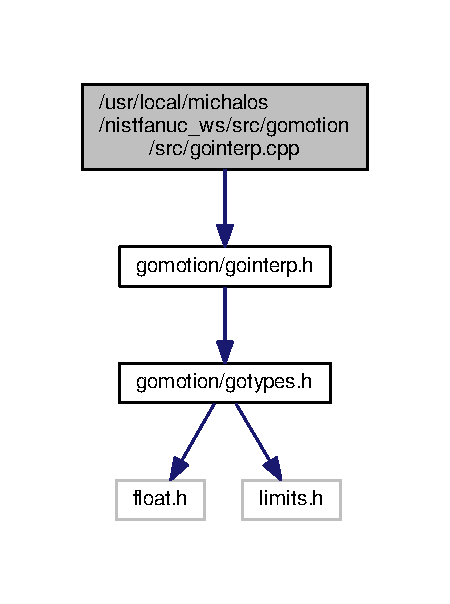
\includegraphics[width=216pt]{d3/dc5/gointerp_8cpp__incl}
\end{center}
\end{figure}
\subsection*{Namespaces}
\begin{DoxyCompactItemize}
\item 
\hyperlink{namespacegomotion}{gomotion}
\end{DoxyCompactItemize}

\hypertarget{gomath_8cpp}{\section{/usr/local/michalos/nistfanuc\-\_\-ws/src/gomotion/src/gomath.cpp File Reference}
\label{gomath_8cpp}\index{/usr/local/michalos/nistfanuc\-\_\-ws/src/gomotion/src/gomath.\-cpp@{/usr/local/michalos/nistfanuc\-\_\-ws/src/gomotion/src/gomath.\-cpp}}
}
{\ttfamily \#include $<$stdio.\-h$>$}\\*
{\ttfamily \#include $<$stddef.\-h$>$}\\*
{\ttfamily \#include $<$math.\-h$>$}\\*
{\ttfamily \#include \char`\"{}gomotion/gotypes.\-h\char`\"{}}\\*
{\ttfamily \#include \char`\"{}gomotion/gomath.\-h\char`\"{}}\\*
Include dependency graph for gomath.\-cpp\-:\nopagebreak
\begin{figure}[H]
\begin{center}
\leavevmode
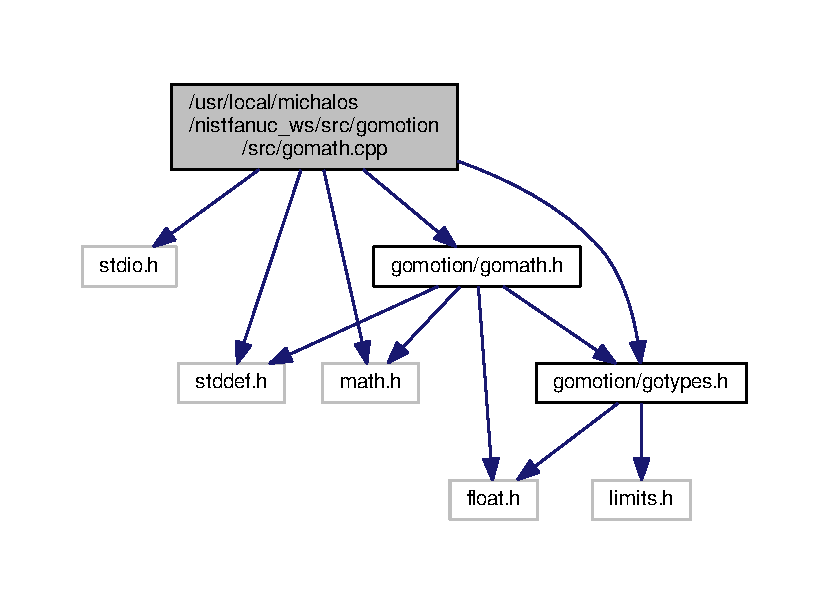
\includegraphics[width=350pt]{d8/d51/gomath_8cpp__incl}
\end{center}
\end{figure}
\subsection*{Namespaces}
\begin{DoxyCompactItemize}
\item 
\hyperlink{namespacegomotion}{gomotion}
\end{DoxyCompactItemize}
\subsection*{Macros}
\begin{DoxyCompactItemize}
\item 
\#define \hyperlink{gomath_8cpp_ac956787f2d378717b55c6a9fd64692f4}{C\-B\-R\-T\-\_\-\-I\-S\-\_\-\-P\-O\-W}
\item 
\#define \hyperlink{gomath_8cpp_ac89d5f8a358eb8a1abdcd0fcef134f1a}{S\-I\-G\-N}(a, b)~((b) $>$= 0.\-0 ? fabs(a) \-: -\/fabs(a))
\item 
\#define \hyperlink{gomath_8cpp_aad5eb8068a35a474745e25f56e321530}{M\-A\-G2}(a, b)~sqrt((a)$\ast$(a)+(b)$\ast$(b))
\item 
\#define \hyperlink{gomath_8cpp_a3f96870cadb5ccb844548984fc0c0235}{C\-O\-L\-\_\-\-I\-S\-\_\-\-U\-N\-I\-T}(r)~\hyperlink{gomath_8h_ab72173c33a8f16e8ecec3b552d2f5ba2}{G\-O\-\_\-\-T\-R\-A\-N\-\_\-\-C\-L\-O\-S\-E}(\hyperlink{gomath_8h_a073619c46f05f2b4180948f5e67328aa}{go\-\_\-sq}((r).x) + \hyperlink{gomath_8h_a073619c46f05f2b4180948f5e67328aa}{go\-\_\-sq}((r).y) + \hyperlink{gomath_8h_a073619c46f05f2b4180948f5e67328aa}{go\-\_\-sq}((r).z), 1)
\end{DoxyCompactItemize}
\subsection*{Functions}
\begin{DoxyCompactItemize}
\item 
void \hyperlink{namespacegomotion_a64138f521669da0b06cd5dee3aa427fc}{gomotion\-::sincos} (double x, double $\ast$sx, double $\ast$cx)
\item 
void \hyperlink{namespacegomotion_a085a19f481a6f3f319f644b6dc5fca4b}{gomotion\-::go\-\_\-sincos} (\hyperlink{gotypes_8h_afd666a2393eebd71ee455846ac9def9b}{go\-\_\-real} t, \hyperlink{gotypes_8h_afd666a2393eebd71ee455846ac9def9b}{go\-\_\-real} $\ast$s, \hyperlink{gotypes_8h_afd666a2393eebd71ee455846ac9def9b}{go\-\_\-real} $\ast$c)
\item 
\hyperlink{gotypes_8h_a55d48b38cd959f63c7e8db8337a9792a}{go\-\_\-result} \hyperlink{namespacegomotion_a8bf33ee1ceabf5861cb6d8f7fe685880}{gomotion\-::go\-\_\-asines} (\hyperlink{gotypes_8h_afd666a2393eebd71ee455846ac9def9b}{go\-\_\-real} s, \hyperlink{gotypes_8h_afd666a2393eebd71ee455846ac9def9b}{go\-\_\-real} $\ast$asp, \hyperlink{gotypes_8h_afd666a2393eebd71ee455846ac9def9b}{go\-\_\-real} $\ast$asn)
\item 
\hyperlink{gotypes_8h_a55d48b38cd959f63c7e8db8337a9792a}{go\-\_\-result} \hyperlink{namespacegomotion_a763dfb5f3ead47a101119bc4ef7a9822}{gomotion\-::go\-\_\-acoses} (\hyperlink{gotypes_8h_afd666a2393eebd71ee455846ac9def9b}{go\-\_\-real} c, \hyperlink{gotypes_8h_afd666a2393eebd71ee455846ac9def9b}{go\-\_\-real} $\ast$acp, \hyperlink{gotypes_8h_afd666a2393eebd71ee455846ac9def9b}{go\-\_\-real} $\ast$acn)
\item 
\hyperlink{gotypes_8h_a55d48b38cd959f63c7e8db8337a9792a}{go\-\_\-result} \hyperlink{namespacegomotion_a6af3a55c31db0c4b47aa157de48ae829}{gomotion\-::go\-\_\-atans} (\hyperlink{gotypes_8h_afd666a2393eebd71ee455846ac9def9b}{go\-\_\-real} t, \hyperlink{gotypes_8h_afd666a2393eebd71ee455846ac9def9b}{go\-\_\-real} $\ast$atp, \hyperlink{gotypes_8h_afd666a2393eebd71ee455846ac9def9b}{go\-\_\-real} $\ast$atn)
\item 
\hyperlink{gotypes_8h_afd666a2393eebd71ee455846ac9def9b}{go\-\_\-real} \hyperlink{namespacegomotion_a11b672dbc5c887c373bd7421c4d74744}{gomotion\-::go\-\_\-cbrt} (\hyperlink{gotypes_8h_afd666a2393eebd71ee455846ac9def9b}{go\-\_\-real} x)
\item 
\hyperlink{gotypes_8h_a55d48b38cd959f63c7e8db8337a9792a}{go\-\_\-result} \hyperlink{namespacegomotion_a83b84d0103b59f7ec48a5d50d3633b0d}{gomotion\-::go\-\_\-cart\-\_\-sph\-\_\-convert} (const go\-\_\-cart $\ast$v, go\-\_\-sph $\ast$s)
\item 
\hyperlink{gotypes_8h_a55d48b38cd959f63c7e8db8337a9792a}{go\-\_\-result} \hyperlink{namespacegomotion_a7647c5352af65cc2c74b6ec1543f16dd}{gomotion\-::go\-\_\-cart\-\_\-cyl\-\_\-convert} (const go\-\_\-cart $\ast$v, go\-\_\-cyl $\ast$c)
\item 
\hyperlink{gotypes_8h_a55d48b38cd959f63c7e8db8337a9792a}{go\-\_\-result} \hyperlink{namespacegomotion_a36a8f262d1a993877a8d31f07eff7889}{gomotion\-::go\-\_\-sph\-\_\-cart\-\_\-convert} (const go\-\_\-sph $\ast$s, go\-\_\-cart $\ast$v)
\item 
\hyperlink{gotypes_8h_a55d48b38cd959f63c7e8db8337a9792a}{go\-\_\-result} \hyperlink{namespacegomotion_af03af2d32b5e62c1ead37c2349cc2f46}{gomotion\-::go\-\_\-sph\-\_\-cyl\-\_\-convert} (const go\-\_\-sph $\ast$s, go\-\_\-cyl $\ast$c)
\item 
\hyperlink{gotypes_8h_a55d48b38cd959f63c7e8db8337a9792a}{go\-\_\-result} \hyperlink{namespacegomotion_abeed59a4cd9519af1b4aaed3c116bd39}{gomotion\-::go\-\_\-cyl\-\_\-cart\-\_\-convert} (const go\-\_\-cyl $\ast$c, go\-\_\-cart $\ast$v)
\item 
\hyperlink{gotypes_8h_a55d48b38cd959f63c7e8db8337a9792a}{go\-\_\-result} \hyperlink{namespacegomotion_ab0bdb87e30818c0fb99166f66f04f847}{gomotion\-::go\-\_\-cyl\-\_\-sph\-\_\-convert} (const go\-\_\-cyl $\ast$c, go\-\_\-sph $\ast$s)
\item 
\hyperlink{gotypes_8h_a55d48b38cd959f63c7e8db8337a9792a}{go\-\_\-result} \hyperlink{namespacegomotion_a5241e24d5f0f0202cc947b7abe59c94d}{gomotion\-::go\-\_\-rvec\-\_\-quat\-\_\-convert} (const go\-\_\-rvec $\ast$r, go\-\_\-quat $\ast$q)
\item 
\hyperlink{gotypes_8h_a55d48b38cd959f63c7e8db8337a9792a}{go\-\_\-result} \hyperlink{namespacegomotion_adf77bee641ddc2ab262b5a7c1037b5fb}{gomotion\-::go\-\_\-rvec\-\_\-mat\-\_\-convert} (const go\-\_\-rvec $\ast$r, go\-\_\-mat $\ast$m)
\item 
\hyperlink{gotypes_8h_a55d48b38cd959f63c7e8db8337a9792a}{go\-\_\-result} \hyperlink{namespacegomotion_a55405939228fa6cf1b4e417361e31cf1}{gomotion\-::go\-\_\-rvec\-\_\-zyz\-\_\-convert} (const go\-\_\-rvec $\ast$rvec, go\-\_\-zyz $\ast$zyz)
\item 
\hyperlink{gotypes_8h_a55d48b38cd959f63c7e8db8337a9792a}{go\-\_\-result} \hyperlink{namespacegomotion_a1ba2b7da6d49b4ead52117a0d424cbb0}{gomotion\-::go\-\_\-rvec\-\_\-zyx\-\_\-convert} (const go\-\_\-rvec $\ast$rvec, go\-\_\-zyx $\ast$zyx)
\item 
\hyperlink{gotypes_8h_a55d48b38cd959f63c7e8db8337a9792a}{go\-\_\-result} \hyperlink{namespacegomotion_a9eec26c29c252c49373f7871e573a3ad}{gomotion\-::go\-\_\-rvec\-\_\-rpy\-\_\-convert} (const go\-\_\-rvec $\ast$r, go\-\_\-rpy $\ast$rpy)
\item 
\hyperlink{gotypes_8h_a55d48b38cd959f63c7e8db8337a9792a}{go\-\_\-result} \hyperlink{namespacegomotion_aba2fc0381e9085e8bedcde7c543a0b1a}{gomotion\-::go\-\_\-quat\-\_\-rvec\-\_\-convert} (const go\-\_\-quat $\ast$q, go\-\_\-rvec $\ast$r)
\item 
\hyperlink{gotypes_8h_a55d48b38cd959f63c7e8db8337a9792a}{go\-\_\-result} \hyperlink{namespacegomotion_adb5fb3eb9abe8e8e6a96ec2c5bdf3857}{gomotion\-::go\-\_\-quat\-\_\-mat\-\_\-convert} (const go\-\_\-quat $\ast$q, go\-\_\-mat $\ast$m)
\item 
\hyperlink{gotypes_8h_a55d48b38cd959f63c7e8db8337a9792a}{go\-\_\-result} \hyperlink{namespacegomotion_a7465dd12350d9c9fc9b59ef619796071}{gomotion\-::go\-\_\-quat\-\_\-zyz\-\_\-convert} (const go\-\_\-quat $\ast$q, go\-\_\-zyz $\ast$zyz)
\item 
\hyperlink{gotypes_8h_a55d48b38cd959f63c7e8db8337a9792a}{go\-\_\-result} \hyperlink{namespacegomotion_a4e32c0da5973b4a837a29bcd4f46a166}{gomotion\-::go\-\_\-quat\-\_\-zyx\-\_\-convert} (const go\-\_\-quat $\ast$q, go\-\_\-zyx $\ast$zyx)
\item 
\hyperlink{gotypes_8h_a55d48b38cd959f63c7e8db8337a9792a}{go\-\_\-result} \hyperlink{namespacegomotion_a8c4bdba65a6b7ff8b6201e84ddde1fe2}{gomotion\-::go\-\_\-quat\-\_\-rpy\-\_\-convert} (const go\-\_\-quat $\ast$q, go\-\_\-rpy $\ast$rpy)
\item 
\hyperlink{gotypes_8h_a55d48b38cd959f63c7e8db8337a9792a}{go\-\_\-result} \hyperlink{namespacegomotion_a0ece2b09a5698233266153dad1cc1896}{gomotion\-::go\-\_\-mat\-\_\-rvec\-\_\-convert} (const go\-\_\-mat $\ast$m, go\-\_\-rvec $\ast$r)
\item 
\hyperlink{gotypes_8h_a55d48b38cd959f63c7e8db8337a9792a}{go\-\_\-result} \hyperlink{namespacegomotion_a56227bf3fda923a384a50d848d2c2314}{gomotion\-::go\-\_\-mat\-\_\-quat\-\_\-convert} (const go\-\_\-mat $\ast$m, go\-\_\-quat $\ast$q)
\item 
\hyperlink{gotypes_8h_a55d48b38cd959f63c7e8db8337a9792a}{go\-\_\-result} \hyperlink{namespacegomotion_aad03f6a80af4b6d8f8c39e5af91484bc}{gomotion\-::go\-\_\-mat\-\_\-zyz\-\_\-convert} (const go\-\_\-mat $\ast$m, go\-\_\-zyz $\ast$zyz)
\item 
\hyperlink{gotypes_8h_a55d48b38cd959f63c7e8db8337a9792a}{go\-\_\-result} \hyperlink{namespacegomotion_ab6def00d51644dc86a0aad564b029ce3}{gomotion\-::go\-\_\-mat\-\_\-zyx\-\_\-convert} (const go\-\_\-mat $\ast$m, go\-\_\-zyx $\ast$zyx)
\item 
\hyperlink{gotypes_8h_a55d48b38cd959f63c7e8db8337a9792a}{go\-\_\-result} \hyperlink{namespacegomotion_ac8969285bc78a45cc21064577803c758}{gomotion\-::go\-\_\-mat\-\_\-xyz\-\_\-convert} (const go\-\_\-mat $\ast$m, go\-\_\-xyz $\ast$xyz)
\item 
\hyperlink{gotypes_8h_a55d48b38cd959f63c7e8db8337a9792a}{go\-\_\-result} \hyperlink{namespacegomotion_ae3d47ff3b11c3be6ec86196b5acca01f}{gomotion\-::go\-\_\-mat\-\_\-rpy\-\_\-convert} (const go\-\_\-mat $\ast$m, go\-\_\-rpy $\ast$rpy)
\item 
\hyperlink{gotypes_8h_a55d48b38cd959f63c7e8db8337a9792a}{go\-\_\-result} \hyperlink{namespacegomotion_ad53feb4160060f91e636345961c12c1d}{gomotion\-::go\-\_\-zyz\-\_\-rvec\-\_\-convert} (const go\-\_\-zyz $\ast$zyz, go\-\_\-rvec $\ast$r)
\item 
\hyperlink{gotypes_8h_a55d48b38cd959f63c7e8db8337a9792a}{go\-\_\-result} \hyperlink{namespacegomotion_ad0211d9ce3c6f9e8fbbe80a184b15d9e}{gomotion\-::go\-\_\-zyz\-\_\-quat\-\_\-convert} (const go\-\_\-zyz $\ast$zyz, go\-\_\-quat $\ast$q)
\item 
\hyperlink{gotypes_8h_a55d48b38cd959f63c7e8db8337a9792a}{go\-\_\-result} \hyperlink{namespacegomotion_a4d8ad1df8907c07480486bc9284f3cfa}{gomotion\-::go\-\_\-zyz\-\_\-mat\-\_\-convert} (const go\-\_\-zyz $\ast$zyz, go\-\_\-mat $\ast$m)
\item 
\hyperlink{gotypes_8h_a55d48b38cd959f63c7e8db8337a9792a}{go\-\_\-result} \hyperlink{namespacegomotion_a132d8bf451632c63d152a70ac9e55824}{gomotion\-::go\-\_\-zyz\-\_\-zyx\-\_\-convert} (const go\-\_\-zyz $\ast$zyz, go\-\_\-zyx $\ast$zyx)
\item 
\hyperlink{gotypes_8h_a55d48b38cd959f63c7e8db8337a9792a}{go\-\_\-result} \hyperlink{namespacegomotion_a186e9aa386fc471351cc8f3d819730f7}{gomotion\-::go\-\_\-zyz\-\_\-rpy\-\_\-convert} (const go\-\_\-zyz $\ast$zyz, go\-\_\-rpy $\ast$rpy)
\item 
\hyperlink{gotypes_8h_a55d48b38cd959f63c7e8db8337a9792a}{go\-\_\-result} \hyperlink{namespacegomotion_a9c449c8dc1828671f0acc40ace796d68}{gomotion\-::go\-\_\-zyx\-\_\-rvec\-\_\-convert} (const go\-\_\-zyx $\ast$zyx, go\-\_\-rvec $\ast$r)
\item 
\hyperlink{gotypes_8h_a55d48b38cd959f63c7e8db8337a9792a}{go\-\_\-result} \hyperlink{namespacegomotion_a0f27fd09f8d74304db6e9ca8185a9623}{gomotion\-::go\-\_\-zyx\-\_\-quat\-\_\-convert} (const go\-\_\-zyx $\ast$zyx, go\-\_\-quat $\ast$q)
\item 
\hyperlink{gotypes_8h_a55d48b38cd959f63c7e8db8337a9792a}{go\-\_\-result} \hyperlink{namespacegomotion_a70010a8b112dc746b53c5e8e6afa9637}{gomotion\-::go\-\_\-zyx\-\_\-mat\-\_\-convert} (const go\-\_\-zyx $\ast$zyx, go\-\_\-mat $\ast$m)
\item 
\hyperlink{gotypes_8h_a55d48b38cd959f63c7e8db8337a9792a}{go\-\_\-result} \hyperlink{namespacegomotion_a586afaa4f9497b0525555968aa3ae0b5}{gomotion\-::go\-\_\-zyx\-\_\-zyz\-\_\-convert} (const go\-\_\-zyx $\ast$zyx, go\-\_\-zyz $\ast$zyz)
\item 
\hyperlink{gotypes_8h_a55d48b38cd959f63c7e8db8337a9792a}{go\-\_\-result} \hyperlink{namespacegomotion_a484efc550824656f71a960fc3cab296d}{gomotion\-::go\-\_\-zyx\-\_\-rpy\-\_\-convert} (const go\-\_\-zyx $\ast$zyx, go\-\_\-rpy $\ast$rpy)
\item 
\hyperlink{gotypes_8h_a55d48b38cd959f63c7e8db8337a9792a}{go\-\_\-result} \hyperlink{namespacegomotion_adb2a7f9cf2609a75afa30093009c58f9}{gomotion\-::go\-\_\-xyz\-\_\-mat\-\_\-convert} (const go\-\_\-xyz $\ast$xyz, go\-\_\-mat $\ast$m)
\item 
\hyperlink{gotypes_8h_a55d48b38cd959f63c7e8db8337a9792a}{go\-\_\-result} \hyperlink{namespacegomotion_ac5ffecbde0428a84dbb839ed6d19600c}{gomotion\-::go\-\_\-rpy\-\_\-rvec\-\_\-convert} (const go\-\_\-rpy $\ast$rpy, go\-\_\-rvec $\ast$rvec)
\item 
\hyperlink{gotypes_8h_a55d48b38cd959f63c7e8db8337a9792a}{go\-\_\-result} \hyperlink{namespacegomotion_a220f82039af859bfd9413107e7fbdf13}{gomotion\-::go\-\_\-rpy\-\_\-quat\-\_\-convert} (const go\-\_\-rpy $\ast$rpy, go\-\_\-quat $\ast$quat)
\item 
\hyperlink{gotypes_8h_a55d48b38cd959f63c7e8db8337a9792a}{go\-\_\-result} \hyperlink{namespacegomotion_a40757f3f8ff59d8879108d052ed087aa}{gomotion\-::go\-\_\-rpy\-\_\-mat\-\_\-convert} (const go\-\_\-rpy $\ast$rpy, go\-\_\-mat $\ast$m)
\item 
\hyperlink{gotypes_8h_a55d48b38cd959f63c7e8db8337a9792a}{go\-\_\-result} \hyperlink{namespacegomotion_ab5c106fe70eeb7dcf83243f83b08bb98}{gomotion\-::go\-\_\-rpy\-\_\-zyz\-\_\-convert} (const go\-\_\-rpy $\ast$rpy, go\-\_\-zyz $\ast$zyz)
\item 
\hyperlink{gotypes_8h_a55d48b38cd959f63c7e8db8337a9792a}{go\-\_\-result} \hyperlink{namespacegomotion_abd91c890da5def1b8d92ecea36d35361}{gomotion\-::go\-\_\-rpy\-\_\-zyx\-\_\-convert} (const go\-\_\-rpy $\ast$rpy, go\-\_\-zyx $\ast$zyx)
\item 
\hyperlink{gotypes_8h_a55d48b38cd959f63c7e8db8337a9792a}{go\-\_\-result} \hyperlink{namespacegomotion_a6d4f9130f4b766bf3e1c9023fe61c9ae}{gomotion\-::go\-\_\-uxz\-\_\-mat\-\_\-convert} (const go\-\_\-uxz $\ast$uxz, go\-\_\-mat $\ast$mat)
\item 
\hyperlink{gotypes_8h_a55d48b38cd959f63c7e8db8337a9792a}{go\-\_\-result} \hyperlink{namespacegomotion_ada32e9e6e533e94cc1dafaa88d584578}{gomotion\-::go\-\_\-mat\-\_\-uxz\-\_\-convert} (const go\-\_\-mat $\ast$mat, go\-\_\-uxz $\ast$uxz)
\item 
go\-\_\-pose \hyperlink{namespacegomotion_a71730b5182346e2fe15337c358013fca}{gomotion\-::go\-\_\-pose\-\_\-this} (\hyperlink{gotypes_8h_afd666a2393eebd71ee455846ac9def9b}{go\-\_\-real} x, \hyperlink{gotypes_8h_afd666a2393eebd71ee455846ac9def9b}{go\-\_\-real} y, \hyperlink{gotypes_8h_afd666a2393eebd71ee455846ac9def9b}{go\-\_\-real} z, \hyperlink{gotypes_8h_afd666a2393eebd71ee455846ac9def9b}{go\-\_\-real} rs, \hyperlink{gotypes_8h_afd666a2393eebd71ee455846ac9def9b}{go\-\_\-real} rx, \hyperlink{gotypes_8h_afd666a2393eebd71ee455846ac9def9b}{go\-\_\-real} ry, \hyperlink{gotypes_8h_afd666a2393eebd71ee455846ac9def9b}{go\-\_\-real} rz)
\item 
go\-\_\-cart \hyperlink{namespacegomotion_aadcf705cf7a6b2a33fb3fb65f5b1a517}{gomotion\-::go\-\_\-cart\-\_\-zero} (void)
\item 
go\-\_\-quat \hyperlink{namespacegomotion_abfb9197b7cceb73fdd68bad553cba624}{gomotion\-::go\-\_\-quat\-\_\-identity} (void)
\item 
go\-\_\-pose \hyperlink{namespacegomotion_ab1257b2f7a291d528ea01466abff5ac8}{gomotion\-::go\-\_\-pose\-\_\-identity} (void)
\item 
\hyperlink{gotypes_8h_a55d48b38cd959f63c7e8db8337a9792a}{go\-\_\-result} \hyperlink{namespacegomotion_ae9423c9f1b2aaf9c6939ed15588f2f25}{gomotion\-::go\-\_\-pose\-\_\-hom\-\_\-convert} (const go\-\_\-pose $\ast$p, go\-\_\-hom $\ast$h)
\item 
\hyperlink{gotypes_8h_a55d48b38cd959f63c7e8db8337a9792a}{go\-\_\-result} \hyperlink{namespacegomotion_a869b48a3a49883c182f73645cc0d2f9e}{gomotion\-::go\-\_\-hom\-\_\-pose\-\_\-convert} (const go\-\_\-hom $\ast$h, go\-\_\-pose $\ast$p)
\item 
\hyperlink{gotypes_8h_a55d48b38cd959f63c7e8db8337a9792a}{go\-\_\-result} \hyperlink{namespacegomotion_a055754ba16cfa9577b99cbe659373308}{gomotion\-::go\-\_\-cart\-\_\-rvec\-\_\-convert} (const go\-\_\-cart $\ast$cart, go\-\_\-rvec $\ast$rvec)
\item 
\hyperlink{gotypes_8h_a55d48b38cd959f63c7e8db8337a9792a}{go\-\_\-result} \hyperlink{namespacegomotion_a20ddc08f42a87ab4d96a53e0670a4384}{gomotion\-::go\-\_\-rvec\-\_\-cart\-\_\-convert} (const go\-\_\-rvec $\ast$rvec, go\-\_\-cart $\ast$cart)
\item 
\hyperlink{gotypes_8h_ae890d9a0ddecc0d3073622cc4312092d}{go\-\_\-flag} \hyperlink{namespacegomotion_aa971bf43a465567a0dd24c4ff38d8054}{gomotion\-::go\-\_\-cart\-\_\-cart\-\_\-compare} (const go\-\_\-cart $\ast$v1, const go\-\_\-cart $\ast$v2)
\item 
\hyperlink{gotypes_8h_a55d48b38cd959f63c7e8db8337a9792a}{go\-\_\-result} \hyperlink{namespacegomotion_aaa7f752392e7056e3636924a001a8731}{gomotion\-::go\-\_\-cart\-\_\-cart\-\_\-dot} (const go\-\_\-cart $\ast$v1, const go\-\_\-cart $\ast$v2, \hyperlink{gotypes_8h_afd666a2393eebd71ee455846ac9def9b}{go\-\_\-real} $\ast$d)
\item 
\hyperlink{gotypes_8h_a55d48b38cd959f63c7e8db8337a9792a}{go\-\_\-result} \hyperlink{namespacegomotion_af03c22a87699451903458ebab6fa9027}{gomotion\-::go\-\_\-cart\-\_\-cart\-\_\-cross} (const go\-\_\-cart $\ast$v1, const go\-\_\-cart $\ast$v2, go\-\_\-cart $\ast$vout)
\item 
\hyperlink{gotypes_8h_a55d48b38cd959f63c7e8db8337a9792a}{go\-\_\-result} \hyperlink{namespacegomotion_a03050d33c64c2a687e282ceb53645235}{gomotion\-::go\-\_\-cart\-\_\-mag} (const go\-\_\-cart $\ast$v, \hyperlink{gotypes_8h_afd666a2393eebd71ee455846ac9def9b}{go\-\_\-real} $\ast$d)
\item 
\hyperlink{gotypes_8h_a55d48b38cd959f63c7e8db8337a9792a}{go\-\_\-result} \hyperlink{namespacegomotion_aa1876c9e617115a9c17664697606f907}{gomotion\-::go\-\_\-cart\-\_\-magsq} (const go\-\_\-cart $\ast$v, \hyperlink{gotypes_8h_afd666a2393eebd71ee455846ac9def9b}{go\-\_\-real} $\ast$d)
\item 
\hyperlink{gotypes_8h_ae890d9a0ddecc0d3073622cc4312092d}{go\-\_\-flag} \hyperlink{namespacegomotion_a4d4b8ab00527c875ca629e6d14b3d94b}{gomotion\-::go\-\_\-cart\-\_\-cart\-\_\-par} (const go\-\_\-cart $\ast$v1, const go\-\_\-cart $\ast$v2)
\item 
\hyperlink{gotypes_8h_ae890d9a0ddecc0d3073622cc4312092d}{go\-\_\-flag} \hyperlink{namespacegomotion_a6b5b67f7dd77ae8de4b73793b8a12ebb}{gomotion\-::go\-\_\-cart\-\_\-cart\-\_\-perp} (const go\-\_\-cart $\ast$v1, const go\-\_\-cart $\ast$v2)
\item 
\hyperlink{gotypes_8h_a55d48b38cd959f63c7e8db8337a9792a}{go\-\_\-result} \hyperlink{namespacegomotion_a2530a89b71ef809648025aff2374021d}{gomotion\-::go\-\_\-cart\-\_\-cart\-\_\-disp} (const go\-\_\-cart $\ast$v1, const go\-\_\-cart $\ast$v2, \hyperlink{gotypes_8h_afd666a2393eebd71ee455846ac9def9b}{go\-\_\-real} $\ast$d)
\item 
\hyperlink{gotypes_8h_a55d48b38cd959f63c7e8db8337a9792a}{go\-\_\-result} \hyperlink{namespacegomotion_a52109f281a73888cae9a5c91b192d06d}{gomotion\-::go\-\_\-cart\-\_\-cart\-\_\-add} (const go\-\_\-cart $\ast$v1, const go\-\_\-cart $\ast$v2, go\-\_\-cart $\ast$vout)
\item 
\hyperlink{gotypes_8h_a55d48b38cd959f63c7e8db8337a9792a}{go\-\_\-result} \hyperlink{namespacegomotion_a967e5544042ebcc17f55e15d406d703c}{gomotion\-::go\-\_\-cart\-\_\-cart\-\_\-sub} (const go\-\_\-cart $\ast$v1, const go\-\_\-cart $\ast$v2, go\-\_\-cart $\ast$vout)
\item 
\hyperlink{gotypes_8h_a55d48b38cd959f63c7e8db8337a9792a}{go\-\_\-result} \hyperlink{namespacegomotion_ae93c6dcde94e08e775a1ef34d0b2b2bc}{gomotion\-::go\-\_\-cart\-\_\-scale\-\_\-mult} (const go\-\_\-cart $\ast$v1, \hyperlink{gotypes_8h_afd666a2393eebd71ee455846ac9def9b}{go\-\_\-real} d, go\-\_\-cart $\ast$vout)
\item 
\hyperlink{gotypes_8h_a55d48b38cd959f63c7e8db8337a9792a}{go\-\_\-result} \hyperlink{namespacegomotion_a8180073b70336b3d2d4191502b443eeb}{gomotion\-::go\-\_\-cart\-\_\-neg} (const go\-\_\-cart $\ast$v1, go\-\_\-cart $\ast$vout)
\item 
\hyperlink{gotypes_8h_a55d48b38cd959f63c7e8db8337a9792a}{go\-\_\-result} \hyperlink{namespacegomotion_abca14b53436057a03c29ca458e8850c1}{gomotion\-::go\-\_\-cart\-\_\-unit} (const go\-\_\-cart $\ast$v, go\-\_\-cart $\ast$vout)
\item 
\hyperlink{gotypes_8h_a55d48b38cd959f63c7e8db8337a9792a}{go\-\_\-result} \hyperlink{namespacegomotion_a32d016105eb4aa2e32bd75373002378f}{gomotion\-::go\-\_\-cart\-\_\-is\-\_\-norm} (const go\-\_\-cart $\ast$v)
\item 
\hyperlink{gotypes_8h_a55d48b38cd959f63c7e8db8337a9792a}{go\-\_\-result} \hyperlink{namespacegomotion_a28374e45a3f7ec79b8ca7b84efe6617d}{gomotion\-::go\-\_\-cart\-\_\-cart\-\_\-rot} (const go\-\_\-cart $\ast$v1, const go\-\_\-cart $\ast$v2, go\-\_\-quat $\ast$quat)
\item 
\hyperlink{gotypes_8h_a55d48b38cd959f63c7e8db8337a9792a}{go\-\_\-result} \hyperlink{namespacegomotion_a1645b058c53e30ced09d3a3823d2f75e}{gomotion\-::go\-\_\-cart\-\_\-cart\-\_\-proj} (const go\-\_\-cart $\ast$v1, const go\-\_\-cart $\ast$v2, go\-\_\-cart $\ast$vout)
\item 
\hyperlink{gotypes_8h_a55d48b38cd959f63c7e8db8337a9792a}{go\-\_\-result} \hyperlink{namespacegomotion_a8cbb71ceb17e1a4b1894cdcc784f1ad5}{gomotion\-::go\-\_\-cart\-\_\-plane\-\_\-proj} (const go\-\_\-cart $\ast$v, const go\-\_\-cart $\ast$normal, go\-\_\-cart $\ast$vout)
\item 
\hyperlink{gotypes_8h_a55d48b38cd959f63c7e8db8337a9792a}{go\-\_\-result} \hyperlink{namespacegomotion_a86e6cb45fa60161e2c4bf66cbde1db81}{gomotion\-::go\-\_\-cart\-\_\-cart\-\_\-angle} (const go\-\_\-cart $\ast$v1, const go\-\_\-cart $\ast$v2, \hyperlink{gotypes_8h_afd666a2393eebd71ee455846ac9def9b}{go\-\_\-real} $\ast$a)
\item 
\hyperlink{gotypes_8h_a55d48b38cd959f63c7e8db8337a9792a}{go\-\_\-result} \hyperlink{namespacegomotion_a3fb48637adc447f5c57555e71c0b2fc6}{gomotion\-::go\-\_\-cart\-\_\-normal} (const go\-\_\-cart $\ast$v, go\-\_\-cart $\ast$vout)
\item 
\hyperlink{gotypes_8h_a55d48b38cd959f63c7e8db8337a9792a}{go\-\_\-result} \hyperlink{namespacegomotion_a63a410189d7c9ab683eaf974e43c3129}{gomotion\-::go\-\_\-cart\-\_\-centroid} (const go\-\_\-cart $\ast$varray, \hyperlink{gotypes_8h_a7d30f606bb0f58ffe2b3bd71e5c8af5c}{go\-\_\-integer} num, go\-\_\-cart $\ast$centroid)
\item 
\hyperlink{gotypes_8h_a55d48b38cd959f63c7e8db8337a9792a}{go\-\_\-result} \hyperlink{namespacegomotion_ae454fe1815fbe1762ffa012bf0c80f20}{gomotion\-::go\-\_\-cart\-\_\-centroidize} (const go\-\_\-cart $\ast$vinarray, \hyperlink{gotypes_8h_a7d30f606bb0f58ffe2b3bd71e5c8af5c}{go\-\_\-integer} num, go\-\_\-cart $\ast$centroid, go\-\_\-cart $\ast$voutarray)
\item 
go\-\_\-complex \hyperlink{namespacegomotion_aba19101511a09bb95ed8ea329200e9fb}{gomotion\-::go\-\_\-complex\-\_\-add} (go\-\_\-complex z1, go\-\_\-complex z2)
\item 
go\-\_\-complex \hyperlink{namespacegomotion_a1141cb8b10a9d940b608b3d94a097a87}{gomotion\-::go\-\_\-complex\-\_\-sub} (go\-\_\-complex z1, go\-\_\-complex z2)
\item 
go\-\_\-complex \hyperlink{namespacegomotion_a874b524e16324e61277ed6d622868c0e}{gomotion\-::go\-\_\-complex\-\_\-mult} (go\-\_\-complex z1, go\-\_\-complex z2)
\item 
go\-\_\-complex \hyperlink{namespacegomotion_abd437ae7226e562aeb05bca496b40daf}{gomotion\-::go\-\_\-complex\-\_\-inv} (go\-\_\-complex z, \hyperlink{gotypes_8h_a55d48b38cd959f63c7e8db8337a9792a}{go\-\_\-result} $\ast$result)
\item 
go\-\_\-complex \hyperlink{namespacegomotion_aacd8a8f522f7134163ab18985900e799}{gomotion\-::go\-\_\-complex\-\_\-div} (go\-\_\-complex z1, go\-\_\-complex z2, \hyperlink{gotypes_8h_a55d48b38cd959f63c7e8db8337a9792a}{go\-\_\-result} $\ast$result)
\item 
go\-\_\-complex \hyperlink{namespacegomotion_a1052957c9cdfb254dd12c69297f5eb42}{gomotion\-::go\-\_\-complex\-\_\-sq} (go\-\_\-complex z)
\item 
go\-\_\-complex \hyperlink{namespacegomotion_a39801dd54fa663a05160c44e50931d88}{gomotion\-::go\-\_\-complex\-\_\-scale} (go\-\_\-complex z, \hyperlink{gotypes_8h_afd666a2393eebd71ee455846ac9def9b}{go\-\_\-real} scale)
\item 
\hyperlink{gotypes_8h_afd666a2393eebd71ee455846ac9def9b}{go\-\_\-real} \hyperlink{namespacegomotion_ad9cb32ab0226fd47d5aa44067896259b}{gomotion\-::go\-\_\-complex\-\_\-mag} (go\-\_\-complex z)
\item 
\hyperlink{gotypes_8h_afd666a2393eebd71ee455846ac9def9b}{go\-\_\-real} \hyperlink{namespacegomotion_aae2a14a55f37184edfa00e1cf3233a81}{gomotion\-::go\-\_\-complex\-\_\-magsq} (go\-\_\-complex z)
\item 
\hyperlink{gotypes_8h_afd666a2393eebd71ee455846ac9def9b}{go\-\_\-real} \hyperlink{namespacegomotion_a2087eb4a9b3f9a81574b28466cfff247}{gomotion\-::go\-\_\-complex\-\_\-arg} (go\-\_\-complex z)
\item 
void \hyperlink{namespacegomotion_a83691499b7c3d7ab3003a73532d89f2c}{gomotion\-::go\-\_\-complex\-\_\-sqrt} (go\-\_\-complex z, go\-\_\-complex $\ast$z1, go\-\_\-complex $\ast$z2)
\item 
void \hyperlink{namespacegomotion_aa82cab05f61afb7c64c622f9810d6fc0}{gomotion\-::go\-\_\-complex\-\_\-cbrt} (go\-\_\-complex z, go\-\_\-complex $\ast$z1, go\-\_\-complex $\ast$z2, go\-\_\-complex $\ast$z3)
\item 
\hyperlink{gotypes_8h_a55d48b38cd959f63c7e8db8337a9792a}{go\-\_\-result} \hyperlink{namespacegomotion_ad3de720de88b3adacfa18b1d87cfdebb}{gomotion\-::go\-\_\-quadratic\-\_\-solve} (const go\-\_\-quadratic $\ast$quad, go\-\_\-complex $\ast$z1, go\-\_\-complex $\ast$z2)
\item 
\hyperlink{gotypes_8h_a55d48b38cd959f63c7e8db8337a9792a}{go\-\_\-result} \hyperlink{namespacegomotion_a9ac60820934c5a8b4ae3c05c7e125d41}{gomotion\-::go\-\_\-cubic\-\_\-solve} (const go\-\_\-cubic $\ast$cub, go\-\_\-complex $\ast$z1, go\-\_\-complex $\ast$z2, go\-\_\-complex $\ast$z3)
\item 
\hyperlink{gotypes_8h_a55d48b38cd959f63c7e8db8337a9792a}{go\-\_\-result} \hyperlink{namespacegomotion_a3e71624097e1cbd2dced92058930ddf4}{gomotion\-::go\-\_\-quartic\-\_\-solve} (const go\-\_\-quartic $\ast$quart, go\-\_\-complex $\ast$z1, go\-\_\-complex $\ast$z2, go\-\_\-complex $\ast$z3, go\-\_\-complex $\ast$z4)
\item 
\hyperlink{gotypes_8h_a55d48b38cd959f63c7e8db8337a9792a}{go\-\_\-result} \hyperlink{namespacegomotion_a7cb3e7889225e10a664f3a18a4544b6a}{gomotion\-::go\-\_\-tridiag\-\_\-reduce} (\hyperlink{gotypes_8h_afd666a2393eebd71ee455846ac9def9b}{go\-\_\-real} $\ast$$\ast$a, \hyperlink{gotypes_8h_a7d30f606bb0f58ffe2b3bd71e5c8af5c}{go\-\_\-integer} n, \hyperlink{gotypes_8h_afd666a2393eebd71ee455846ac9def9b}{go\-\_\-real} $\ast$d, \hyperlink{gotypes_8h_afd666a2393eebd71ee455846ac9def9b}{go\-\_\-real} $\ast$e)
\item 
\hyperlink{gotypes_8h_a55d48b38cd959f63c7e8db8337a9792a}{go\-\_\-result} \hyperlink{namespacegomotion_a8cdb1cdd1aa1fe79e05cdce767172a43}{gomotion\-::go\-\_\-tridiag\-\_\-ql} (\hyperlink{gotypes_8h_afd666a2393eebd71ee455846ac9def9b}{go\-\_\-real} $\ast$d, \hyperlink{gotypes_8h_afd666a2393eebd71ee455846ac9def9b}{go\-\_\-real} $\ast$e, \hyperlink{gotypes_8h_a7d30f606bb0f58ffe2b3bd71e5c8af5c}{go\-\_\-integer} n, \hyperlink{gotypes_8h_afd666a2393eebd71ee455846ac9def9b}{go\-\_\-real} $\ast$$\ast$z)
\item 
\hyperlink{gotypes_8h_a55d48b38cd959f63c7e8db8337a9792a}{go\-\_\-result} \hyperlink{namespacegomotion_a78b82d69510763b3c86c26bca614e22e}{gomotion\-::go\-\_\-cart\-\_\-cart\-\_\-pose} (const go\-\_\-cart $\ast$v1, const go\-\_\-cart $\ast$v2, go\-\_\-cart $\ast$v1c, go\-\_\-cart $\ast$v2c, \hyperlink{gotypes_8h_a7d30f606bb0f58ffe2b3bd71e5c8af5c}{go\-\_\-integer} num, go\-\_\-pose $\ast$pout)
\item 
\hyperlink{gotypes_8h_a55d48b38cd959f63c7e8db8337a9792a}{go\-\_\-result} \hyperlink{namespacegomotion_a9444ada761a6e8be2db14846b955e276}{gomotion\-::go\-\_\-cart\-\_\-trilaterate} (const go\-\_\-cart $\ast$c1, const go\-\_\-cart $\ast$c2, const go\-\_\-cart $\ast$c3, \hyperlink{gotypes_8h_afd666a2393eebd71ee455846ac9def9b}{go\-\_\-real} l1, \hyperlink{gotypes_8h_afd666a2393eebd71ee455846ac9def9b}{go\-\_\-real} l2, \hyperlink{gotypes_8h_afd666a2393eebd71ee455846ac9def9b}{go\-\_\-real} l3, go\-\_\-cart $\ast$out1, go\-\_\-cart $\ast$out2)
\item 
\hyperlink{gotypes_8h_ae890d9a0ddecc0d3073622cc4312092d}{go\-\_\-flag} \hyperlink{namespacegomotion_a170969f552d3a76100734d6664069c02}{gomotion\-::go\-\_\-rvec\-\_\-rvec\-\_\-compare} (const go\-\_\-rvec $\ast$r1, const go\-\_\-rvec $\ast$r2)
\item 
\hyperlink{gotypes_8h_a55d48b38cd959f63c7e8db8337a9792a}{go\-\_\-result} \hyperlink{namespacegomotion_a4cb3d0febaa9707a5e2978609d195d01}{gomotion\-::go\-\_\-rvec\-\_\-scale\-\_\-mult} (const go\-\_\-rvec $\ast$r, \hyperlink{gotypes_8h_afd666a2393eebd71ee455846ac9def9b}{go\-\_\-real} s, go\-\_\-rvec $\ast$rout)
\item 
\hyperlink{gotypes_8h_a55d48b38cd959f63c7e8db8337a9792a}{go\-\_\-result} \hyperlink{namespacegomotion_ac89b091b7958b0916f0bfffc89022751}{gomotion\-::go\-\_\-rpy\-\_\-cart\-\_\-mult} (const go\-\_\-rpy $\ast$rpy, const go\-\_\-cart $\ast$in, go\-\_\-cart $\ast$out)
\item 
\hyperlink{gotypes_8h_a55d48b38cd959f63c7e8db8337a9792a}{go\-\_\-result} \hyperlink{namespacegomotion_afb64295d1befa9e078204687259d3b6f}{gomotion\-::go\-\_\-mat\-\_\-norm} (const go\-\_\-mat $\ast$mat, go\-\_\-mat $\ast$mout)
\item 
\hyperlink{gotypes_8h_ae890d9a0ddecc0d3073622cc4312092d}{go\-\_\-flag} \hyperlink{namespacegomotion_ad1aa76bab71411b00ce892a6ccd5c046}{gomotion\-::go\-\_\-mat\-\_\-is\-\_\-norm} (const go\-\_\-mat $\ast$m)
\item 
\hyperlink{gotypes_8h_a55d48b38cd959f63c7e8db8337a9792a}{go\-\_\-result} \hyperlink{namespacegomotion_a5a177297f36536f9e1f6c5dcd8564336}{gomotion\-::go\-\_\-mat\-\_\-inv} (const go\-\_\-mat $\ast$m, go\-\_\-mat $\ast$mout)
\item 
\hyperlink{gotypes_8h_a55d48b38cd959f63c7e8db8337a9792a}{go\-\_\-result} \hyperlink{namespacegomotion_a7363f6dc600af28879b1ebaf69d20e5e}{gomotion\-::go\-\_\-mat\-\_\-cart\-\_\-mult} (const go\-\_\-mat $\ast$m, const go\-\_\-cart $\ast$v, go\-\_\-cart $\ast$vout)
\item 
\hyperlink{gotypes_8h_a55d48b38cd959f63c7e8db8337a9792a}{go\-\_\-result} \hyperlink{namespacegomotion_a8d1faf309408b9c06432ddfba0f5bf8f}{gomotion\-::go\-\_\-mat\-\_\-mat\-\_\-mult} (const go\-\_\-mat $\ast$m1, const go\-\_\-mat $\ast$m2, go\-\_\-mat $\ast$mout)
\item 
\hyperlink{gotypes_8h_ae890d9a0ddecc0d3073622cc4312092d}{go\-\_\-flag} \hyperlink{namespacegomotion_a5c86ff088b7e2a5281cb54d083bfada4}{gomotion\-::go\-\_\-quat\-\_\-quat\-\_\-compare} (const go\-\_\-quat $\ast$q1, const go\-\_\-quat $\ast$q2)
\item 
\hyperlink{gotypes_8h_a55d48b38cd959f63c7e8db8337a9792a}{go\-\_\-result} \hyperlink{namespacegomotion_a16e13bdbbe8c3adb4a8c7f30e12a35fa}{gomotion\-::go\-\_\-quat\-\_\-mag} (const go\-\_\-quat $\ast$quat, \hyperlink{gotypes_8h_afd666a2393eebd71ee455846ac9def9b}{go\-\_\-real} $\ast$d)
\item 
\hyperlink{gotypes_8h_a55d48b38cd959f63c7e8db8337a9792a}{go\-\_\-result} \hyperlink{namespacegomotion_a61694fed512375ade28ae77c1ef36f6d}{gomotion\-::go\-\_\-quat\-\_\-unit} (const go\-\_\-quat $\ast$q1, go\-\_\-quat $\ast$qout)
\item 
\hyperlink{gotypes_8h_a55d48b38cd959f63c7e8db8337a9792a}{go\-\_\-result} \hyperlink{namespacegomotion_aa4e00f7f0a0c499da767458ac55269a3}{gomotion\-::go\-\_\-quat\-\_\-norm} (const go\-\_\-quat $\ast$q1, go\-\_\-quat $\ast$qout)
\item 
\hyperlink{gotypes_8h_a55d48b38cd959f63c7e8db8337a9792a}{go\-\_\-result} \hyperlink{namespacegomotion_aa10a1f4ea91bf33c82fa1e687c35acaa}{gomotion\-::go\-\_\-quat\-\_\-inv} (const go\-\_\-quat $\ast$q1, go\-\_\-quat $\ast$qout)
\item 
\hyperlink{gotypes_8h_ae890d9a0ddecc0d3073622cc4312092d}{go\-\_\-flag} \hyperlink{namespacegomotion_a0320bf206aa58e6f3587be2069704de8}{gomotion\-::go\-\_\-quat\-\_\-is\-\_\-norm} (const go\-\_\-quat $\ast$q1)
\item 
\hyperlink{gotypes_8h_a55d48b38cd959f63c7e8db8337a9792a}{go\-\_\-result} \hyperlink{namespacegomotion_a8ecc295000058285ea22d2f2c8bafb5a}{gomotion\-::go\-\_\-quat\-\_\-scale\-\_\-mult} (const go\-\_\-quat $\ast$q, \hyperlink{gotypes_8h_afd666a2393eebd71ee455846ac9def9b}{go\-\_\-real} s, go\-\_\-quat $\ast$qout)
\item 
\hyperlink{gotypes_8h_a55d48b38cd959f63c7e8db8337a9792a}{go\-\_\-result} \hyperlink{namespacegomotion_ac32c196f6f682de23e5e828c601977a6}{gomotion\-::go\-\_\-quat\-\_\-quat\-\_\-mult} (const go\-\_\-quat $\ast$q1, const go\-\_\-quat $\ast$q2, go\-\_\-quat $\ast$qout)
\item 
\hyperlink{gotypes_8h_a55d48b38cd959f63c7e8db8337a9792a}{go\-\_\-result} \hyperlink{namespacegomotion_a7d60b7e9ba5faa7e59486698407dae20}{gomotion\-::go\-\_\-quat\-\_\-cart\-\_\-mult} (const go\-\_\-quat $\ast$q1, const go\-\_\-cart $\ast$v2, go\-\_\-cart $\ast$vout)
\item 
\hyperlink{gotypes_8h_ae890d9a0ddecc0d3073622cc4312092d}{go\-\_\-flag} \hyperlink{namespacegomotion_a3fb737a5f90354bd0809963797573769}{gomotion\-::go\-\_\-pose\-\_\-pose\-\_\-compare} (const go\-\_\-pose $\ast$p1, const go\-\_\-pose $\ast$p2)
\item 
\hyperlink{gotypes_8h_a55d48b38cd959f63c7e8db8337a9792a}{go\-\_\-result} \hyperlink{namespacegomotion_a7659bf73ec87a38607995939ca405cc5}{gomotion\-::go\-\_\-pose\-\_\-inv} (const go\-\_\-pose $\ast$p1, go\-\_\-pose $\ast$p2)
\item 
\hyperlink{gotypes_8h_a55d48b38cd959f63c7e8db8337a9792a}{go\-\_\-result} \hyperlink{namespacegomotion_a8fddcbebee69b64a2536721c33087e3c}{gomotion\-::go\-\_\-pose\-\_\-cart\-\_\-mult} (const go\-\_\-pose $\ast$p1, const go\-\_\-cart $\ast$v2, go\-\_\-cart $\ast$vout)
\item 
\hyperlink{gotypes_8h_a55d48b38cd959f63c7e8db8337a9792a}{go\-\_\-result} \hyperlink{namespacegomotion_a67d9fb285388234b9ea790849952b965}{gomotion\-::go\-\_\-pose\-\_\-pose\-\_\-mult} (const go\-\_\-pose $\ast$p1, const go\-\_\-pose $\ast$p2, go\-\_\-pose $\ast$pout)
\item 
\hyperlink{gotypes_8h_a55d48b38cd959f63c7e8db8337a9792a}{go\-\_\-result} \hyperlink{namespacegomotion_a1cca8106f4bb9eb3822b5fb356164c3e}{gomotion\-::go\-\_\-pose\-\_\-scale\-\_\-mult} (const go\-\_\-pose $\ast$p1, \hyperlink{gotypes_8h_afd666a2393eebd71ee455846ac9def9b}{go\-\_\-real} s, go\-\_\-pose $\ast$pout)
\item 
\hyperlink{gotypes_8h_a55d48b38cd959f63c7e8db8337a9792a}{go\-\_\-result} \hyperlink{namespacegomotion_a4662e2daf4c61f269935131eefda1d2a}{gomotion\-::go\-\_\-pose\-\_\-pose\-\_\-interp} (\hyperlink{gotypes_8h_afd666a2393eebd71ee455846ac9def9b}{go\-\_\-real} t1, const go\-\_\-pose $\ast$p1, \hyperlink{gotypes_8h_afd666a2393eebd71ee455846ac9def9b}{go\-\_\-real} t2, const go\-\_\-pose $\ast$p2, \hyperlink{gotypes_8h_afd666a2393eebd71ee455846ac9def9b}{go\-\_\-real} t3, go\-\_\-pose $\ast$p3)
\item 
\hyperlink{gotypes_8h_a55d48b38cd959f63c7e8db8337a9792a}{go\-\_\-result} \hyperlink{namespacegomotion_aafe2ece40a4ac948cd8d07c069ef0434}{gomotion\-::go\-\_\-hom\-\_\-inv} (const go\-\_\-hom $\ast$h1, go\-\_\-hom $\ast$h2)
\item 
\hyperlink{gotypes_8h_a55d48b38cd959f63c7e8db8337a9792a}{go\-\_\-result} \hyperlink{namespacegomotion_a7b65e9509700ef5c058f152c21b5643c}{gomotion\-::go\-\_\-hom\-\_\-hom\-\_\-mult} (const go\-\_\-hom $\ast$h1, const go\-\_\-hom $\ast$h2, go\-\_\-hom $\ast$hout)
\item 
\hyperlink{gotypes_8h_a55d48b38cd959f63c7e8db8337a9792a}{go\-\_\-result} \hyperlink{namespacegomotion_a02133a76965d9e2111eca88ef5961f81}{gomotion\-::go\-\_\-pose\-\_\-vel\-\_\-mult} (const go\-\_\-pose $\ast$pose, const go\-\_\-vel $\ast$vel, go\-\_\-vel $\ast$out)
\item 
\hyperlink{gotypes_8h_a55d48b38cd959f63c7e8db8337a9792a}{go\-\_\-result} \hyperlink{namespacegomotion_aac937b55b391d0b7565719d301389bc6}{gomotion\-::go\-\_\-line\-\_\-from\-\_\-point\-\_\-direction} (const go\-\_\-cart $\ast$point, const go\-\_\-cart $\ast$direction, go\-\_\-line $\ast$line)
\item 
\hyperlink{gotypes_8h_a55d48b38cd959f63c7e8db8337a9792a}{go\-\_\-result} \hyperlink{namespacegomotion_a13ea203461728105546fe4af4083f6ba}{gomotion\-::go\-\_\-line\-\_\-from\-\_\-points} (const go\-\_\-cart $\ast$point1, const go\-\_\-cart $\ast$point2, go\-\_\-line $\ast$line)
\item 
\hyperlink{gotypes_8h_a55d48b38cd959f63c7e8db8337a9792a}{go\-\_\-result} \hyperlink{namespacegomotion_a239960b865134d678928490b91100702}{gomotion\-::go\-\_\-line\-\_\-from\-\_\-planes} (const go\-\_\-plane $\ast$plane1, const go\-\_\-plane $\ast$plane2, go\-\_\-line $\ast$line)
\item 
\hyperlink{gotypes_8h_ae890d9a0ddecc0d3073622cc4312092d}{go\-\_\-flag} \hyperlink{namespacegomotion_a5b409973e65746e7698f0afbcf9183de}{gomotion\-::go\-\_\-line\-\_\-line\-\_\-compare} (const go\-\_\-line $\ast$line1, const go\-\_\-line $\ast$line2)
\item 
\hyperlink{gotypes_8h_a55d48b38cd959f63c7e8db8337a9792a}{go\-\_\-result} \hyperlink{namespacegomotion_a301c198b3225ff73ad5598c046166a4a}{gomotion\-::go\-\_\-line\-\_\-evaluate} (const go\-\_\-line $\ast$line, \hyperlink{gotypes_8h_afd666a2393eebd71ee455846ac9def9b}{go\-\_\-real} d, go\-\_\-cart $\ast$point)
\item 
\hyperlink{gotypes_8h_a55d48b38cd959f63c7e8db8337a9792a}{go\-\_\-result} \hyperlink{namespacegomotion_a2144eb2d183b1aaf60549d66ae7dfcf6}{gomotion\-::go\-\_\-point\-\_\-line\-\_\-distance} (const go\-\_\-cart $\ast$point, const go\-\_\-line $\ast$line, \hyperlink{gotypes_8h_afd666a2393eebd71ee455846ac9def9b}{go\-\_\-real} $\ast$distance)
\item 
\hyperlink{gotypes_8h_a55d48b38cd959f63c7e8db8337a9792a}{go\-\_\-result} \hyperlink{namespacegomotion_a36bd2c5167f64cc51da6bdf3dbdb4116}{gomotion\-::go\-\_\-point\-\_\-line\-\_\-proj} (const go\-\_\-cart $\ast$point, const go\-\_\-line $\ast$line, go\-\_\-cart $\ast$pout)
\item 
\hyperlink{gotypes_8h_a55d48b38cd959f63c7e8db8337a9792a}{go\-\_\-result} \hyperlink{namespacegomotion_a79d749aa4142b2ee2e135f46a6656f21}{gomotion\-::go\-\_\-point\-\_\-plane\-\_\-proj} (const go\-\_\-cart $\ast$point, const go\-\_\-plane $\ast$plane, go\-\_\-cart $\ast$proj)
\item 
\hyperlink{gotypes_8h_a55d48b38cd959f63c7e8db8337a9792a}{go\-\_\-result} \hyperlink{namespacegomotion_a120a912e2b439a904744d980b62867aa}{gomotion\-::go\-\_\-line\-\_\-plane\-\_\-proj} (const go\-\_\-line $\ast$line, const go\-\_\-plane $\ast$plane, go\-\_\-line $\ast$proj)
\item 
\hyperlink{gotypes_8h_a55d48b38cd959f63c7e8db8337a9792a}{go\-\_\-result} \hyperlink{namespacegomotion_abffde2f69bd2e58d2b099558e892661e}{gomotion\-::go\-\_\-plane\-\_\-from\-\_\-point\-\_\-normal} (const go\-\_\-cart $\ast$point, const go\-\_\-cart $\ast$normal, go\-\_\-plane $\ast$plane)
\item 
\hyperlink{gotypes_8h_a55d48b38cd959f63c7e8db8337a9792a}{go\-\_\-result} \hyperlink{namespacegomotion_a62472d69cf3770531052efa51d42d139}{gomotion\-::go\-\_\-plane\-\_\-from\-\_\-abcd} (\hyperlink{gotypes_8h_afd666a2393eebd71ee455846ac9def9b}{go\-\_\-real} A, \hyperlink{gotypes_8h_afd666a2393eebd71ee455846ac9def9b}{go\-\_\-real} B, \hyperlink{gotypes_8h_afd666a2393eebd71ee455846ac9def9b}{go\-\_\-real} C, \hyperlink{gotypes_8h_afd666a2393eebd71ee455846ac9def9b}{go\-\_\-real} D, go\-\_\-plane $\ast$plane)
\item 
\hyperlink{gotypes_8h_a55d48b38cd959f63c7e8db8337a9792a}{go\-\_\-result} \hyperlink{namespacegomotion_aebc299a30f9b6bab3221df9381691a7a}{gomotion\-::go\-\_\-plane\-\_\-from\-\_\-points} (const go\-\_\-cart $\ast$point1, const go\-\_\-cart $\ast$point2, const go\-\_\-cart $\ast$point3, go\-\_\-plane $\ast$plane)
\item 
\hyperlink{gotypes_8h_a55d48b38cd959f63c7e8db8337a9792a}{go\-\_\-result} \hyperlink{namespacegomotion_a3f05dac5f9be2e82ec390a70d03ea058}{gomotion\-::go\-\_\-plane\-\_\-from\-\_\-point\-\_\-line} (const go\-\_\-cart $\ast$point, const go\-\_\-line $\ast$line, go\-\_\-plane $\ast$plane)
\item 
\hyperlink{gotypes_8h_ae890d9a0ddecc0d3073622cc4312092d}{go\-\_\-flag} \hyperlink{namespacegomotion_a522b91008a97b01ef46291dcd5bcb2e0}{gomotion\-::go\-\_\-plane\-\_\-plane\-\_\-compare} (const go\-\_\-plane $\ast$plane1, const go\-\_\-plane $\ast$plane2)
\item 
\hyperlink{gotypes_8h_a55d48b38cd959f63c7e8db8337a9792a}{go\-\_\-result} \hyperlink{namespacegomotion_a9e922da92de4833b51a5867e8fd99cca}{gomotion\-::go\-\_\-point\-\_\-plane\-\_\-distance} (const go\-\_\-cart $\ast$point, const go\-\_\-plane $\ast$plane, \hyperlink{gotypes_8h_afd666a2393eebd71ee455846ac9def9b}{go\-\_\-real} $\ast$distance)
\item 
\hyperlink{gotypes_8h_a55d48b38cd959f63c7e8db8337a9792a}{go\-\_\-result} \hyperlink{namespacegomotion_a45d26171e087d7b1abf3664a127d7006}{gomotion\-::go\-\_\-plane\-\_\-evaluate} (const go\-\_\-plane $\ast$plane, \hyperlink{gotypes_8h_afd666a2393eebd71ee455846ac9def9b}{go\-\_\-real} u, \hyperlink{gotypes_8h_afd666a2393eebd71ee455846ac9def9b}{go\-\_\-real} v, go\-\_\-cart $\ast$point)
\item 
\hyperlink{gotypes_8h_a55d48b38cd959f63c7e8db8337a9792a}{go\-\_\-result} \hyperlink{namespacegomotion_a07b423b2ecb498fbdc2cc810ae52980c}{gomotion\-::go\-\_\-line\-\_\-plane\-\_\-intersect} (const go\-\_\-line $\ast$line, const go\-\_\-plane $\ast$plane, go\-\_\-cart $\ast$point, \hyperlink{gotypes_8h_afd666a2393eebd71ee455846ac9def9b}{go\-\_\-real} $\ast$distance)
\item 
\hyperlink{gotypes_8h_afd666a2393eebd71ee455846ac9def9b}{go\-\_\-real} \hyperlink{namespacegomotion_ac58aa8880f6ed18a0ad78b356f579698}{gomotion\-::go\-\_\-get\-\_\-singular\-\_\-epsilon} (void)
\item 
\hyperlink{gotypes_8h_a55d48b38cd959f63c7e8db8337a9792a}{go\-\_\-result} \hyperlink{namespacegomotion_a19aaf652f4b2c5c8c3ea1829d0e2cc99}{gomotion\-::go\-\_\-set\-\_\-singular\-\_\-epsilon} (\hyperlink{gotypes_8h_afd666a2393eebd71ee455846ac9def9b}{go\-\_\-real} epsilon)
\item 
\hyperlink{gotypes_8h_a55d48b38cd959f63c7e8db8337a9792a}{go\-\_\-result} \hyperlink{namespacegomotion_a6c08b09d52c128f06eef43e3a566e0f0}{gomotion\-::ludcmp} (\hyperlink{gotypes_8h_afd666a2393eebd71ee455846ac9def9b}{go\-\_\-real} $\ast$$\ast$a, \hyperlink{gotypes_8h_afd666a2393eebd71ee455846ac9def9b}{go\-\_\-real} $\ast$scratchrow, \hyperlink{gotypes_8h_a7d30f606bb0f58ffe2b3bd71e5c8af5c}{go\-\_\-integer} n, \hyperlink{gotypes_8h_a7d30f606bb0f58ffe2b3bd71e5c8af5c}{go\-\_\-integer} $\ast$indx, \hyperlink{gotypes_8h_afd666a2393eebd71ee455846ac9def9b}{go\-\_\-real} $\ast$d)
\item 
\hyperlink{gotypes_8h_a55d48b38cd959f63c7e8db8337a9792a}{go\-\_\-result} \hyperlink{namespacegomotion_ae0171663e44ea6cee7e420762f3b2b49}{gomotion\-::lubksb} (\hyperlink{gotypes_8h_afd666a2393eebd71ee455846ac9def9b}{go\-\_\-real} $\ast$$\ast$a, \hyperlink{gotypes_8h_a7d30f606bb0f58ffe2b3bd71e5c8af5c}{go\-\_\-integer} n, \hyperlink{gotypes_8h_a7d30f606bb0f58ffe2b3bd71e5c8af5c}{go\-\_\-integer} $\ast$indx, \hyperlink{gotypes_8h_afd666a2393eebd71ee455846ac9def9b}{go\-\_\-real} $\ast$b)
\item 
\hyperlink{gotypes_8h_a55d48b38cd959f63c7e8db8337a9792a}{go\-\_\-result} \hyperlink{namespacegomotion_aa657300121fea0ab47d52c6d7cedc8f7}{gomotion\-::go\-\_\-cart\-\_\-vector\-\_\-convert} (const go\-\_\-cart $\ast$c, \hyperlink{gotypes_8h_afd666a2393eebd71ee455846ac9def9b}{go\-\_\-real} $\ast$v)
\item 
\hyperlink{gotypes_8h_a55d48b38cd959f63c7e8db8337a9792a}{go\-\_\-result} \hyperlink{namespacegomotion_aadbfd671a04f0859d83633fb3884adba}{gomotion\-::go\-\_\-vector\-\_\-cart\-\_\-convert} (const \hyperlink{gotypes_8h_afd666a2393eebd71ee455846ac9def9b}{go\-\_\-real} $\ast$v, go\-\_\-cart $\ast$c)
\item 
\hyperlink{gotypes_8h_a55d48b38cd959f63c7e8db8337a9792a}{go\-\_\-result} \hyperlink{namespacegomotion_aea94351199e643eb32f62ee992e4b2a9}{gomotion\-::go\-\_\-quat\-\_\-matrix\-\_\-convert} (const go\-\_\-quat $\ast$quat, go\-\_\-matrix $\ast$matrix)
\item 
\hyperlink{gotypes_8h_a55d48b38cd959f63c7e8db8337a9792a}{go\-\_\-result} \hyperlink{namespacegomotion_a7fb86f9067e1a6a057ac7244bb06a50c}{gomotion\-::go\-\_\-mat\-\_\-matrix\-\_\-convert} (const go\-\_\-mat $\ast$mat, go\-\_\-matrix $\ast$matrix)
\item 
\hyperlink{gotypes_8h_a55d48b38cd959f63c7e8db8337a9792a}{go\-\_\-result} \hyperlink{namespacegomotion_af1d2ab626e727673e3a170e236b27f27}{gomotion\-::go\-\_\-matrix\-\_\-matrix\-\_\-add} (const go\-\_\-matrix $\ast$a, const go\-\_\-matrix $\ast$b, go\-\_\-matrix $\ast$apb)
\item 
\hyperlink{gotypes_8h_a55d48b38cd959f63c7e8db8337a9792a}{go\-\_\-result} \hyperlink{namespacegomotion_a3812b238fd3884974d1c02c34772d256}{gomotion\-::go\-\_\-matrix\-\_\-matrix\-\_\-copy} (const go\-\_\-matrix $\ast$src, go\-\_\-matrix $\ast$dst)
\item 
\hyperlink{gotypes_8h_a55d48b38cd959f63c7e8db8337a9792a}{go\-\_\-result} \hyperlink{namespacegomotion_a6183caffbd0d82718f15155b31656f0e}{gomotion\-::go\-\_\-matrix\-\_\-matrix\-\_\-mult} (const go\-\_\-matrix $\ast$a, const go\-\_\-matrix $\ast$b, go\-\_\-matrix $\ast$ab)
\item 
\hyperlink{gotypes_8h_a55d48b38cd959f63c7e8db8337a9792a}{go\-\_\-result} \hyperlink{namespacegomotion_aadef0b21be67d00a35d979661ca05b71}{gomotion\-::go\-\_\-matrix\-\_\-vector\-\_\-mult} (const go\-\_\-matrix $\ast$a, const go\-\_\-vector $\ast$v, go\-\_\-vector $\ast$axv)
\item 
\hyperlink{gotypes_8h_a55d48b38cd959f63c7e8db8337a9792a}{go\-\_\-result} \hyperlink{namespacegomotion_af513072af00a07811c442f8a98e93a9c}{gomotion\-::go\-\_\-matrix\-\_\-vector\-\_\-cross} (const go\-\_\-matrix $\ast$a, const go\-\_\-vector $\ast$v, go\-\_\-matrix $\ast$axv)
\item 
\hyperlink{gotypes_8h_a55d48b38cd959f63c7e8db8337a9792a}{go\-\_\-result} \hyperlink{namespacegomotion_a249bea0e6ffc14a6274681b595ad738d}{gomotion\-::go\-\_\-matrix\-\_\-transpose} (const go\-\_\-matrix $\ast$a, go\-\_\-matrix $\ast$at)
\item 
\hyperlink{gotypes_8h_a55d48b38cd959f63c7e8db8337a9792a}{go\-\_\-result} \hyperlink{namespacegomotion_a3e08f14b7f0ace90e71f7526e35a7463}{gomotion\-::go\-\_\-matrix\-\_\-inv} (const go\-\_\-matrix $\ast$m, go\-\_\-matrix $\ast$minv)
\item 
\hyperlink{gotypes_8h_a55d48b38cd959f63c7e8db8337a9792a}{go\-\_\-result} \hyperlink{namespacegomotion_ad60afe8680a8b58625d3b6c104d77bbd}{gomotion\-::go\-\_\-mat3\-\_\-inv} (\hyperlink{gotypes_8h_afd666a2393eebd71ee455846ac9def9b}{go\-\_\-real} a\mbox{[}3\mbox{]}\mbox{[}3\mbox{]}, \hyperlink{gotypes_8h_afd666a2393eebd71ee455846ac9def9b}{go\-\_\-real} ainv\mbox{[}3\mbox{]}\mbox{[}3\mbox{]})
\item 
\hyperlink{gotypes_8h_a55d48b38cd959f63c7e8db8337a9792a}{go\-\_\-result} \hyperlink{namespacegomotion_aec10cf06c1177abebc9b55c77fb6d662}{gomotion\-::go\-\_\-mat3\-\_\-mat3\-\_\-mult} (\hyperlink{gotypes_8h_afd666a2393eebd71ee455846ac9def9b}{go\-\_\-real} a\mbox{[}3\mbox{]}\mbox{[}3\mbox{]}, \hyperlink{gotypes_8h_afd666a2393eebd71ee455846ac9def9b}{go\-\_\-real} b\mbox{[}3\mbox{]}\mbox{[}3\mbox{]}, \hyperlink{gotypes_8h_afd666a2393eebd71ee455846ac9def9b}{go\-\_\-real} axb\mbox{[}3\mbox{]}\mbox{[}3\mbox{]})
\item 
\hyperlink{gotypes_8h_a55d48b38cd959f63c7e8db8337a9792a}{go\-\_\-result} \hyperlink{namespacegomotion_a2f3046912ba704f1aba092455a073172}{gomotion\-::go\-\_\-mat3\-\_\-vec3\-\_\-mult} (\hyperlink{gotypes_8h_afd666a2393eebd71ee455846ac9def9b}{go\-\_\-real} a\mbox{[}3\mbox{]}\mbox{[}3\mbox{]}, \hyperlink{gotypes_8h_afd666a2393eebd71ee455846ac9def9b}{go\-\_\-real} v\mbox{[}3\mbox{]}, \hyperlink{gotypes_8h_afd666a2393eebd71ee455846ac9def9b}{go\-\_\-real} axv\mbox{[}3\mbox{]})
\item 
\hyperlink{gotypes_8h_a55d48b38cd959f63c7e8db8337a9792a}{go\-\_\-result} \hyperlink{namespacegomotion_a85fbe89cb8863fc4dc9d674c56780e8a}{gomotion\-::go\-\_\-mat4\-\_\-inv} (\hyperlink{gotypes_8h_afd666a2393eebd71ee455846ac9def9b}{go\-\_\-real} a\mbox{[}4\mbox{]}\mbox{[}4\mbox{]}, \hyperlink{gotypes_8h_afd666a2393eebd71ee455846ac9def9b}{go\-\_\-real} ainv\mbox{[}4\mbox{]}\mbox{[}4\mbox{]})
\item 
\hyperlink{gotypes_8h_a55d48b38cd959f63c7e8db8337a9792a}{go\-\_\-result} \hyperlink{namespacegomotion_a05e897fff802f77058a689e1dd3c5211}{gomotion\-::go\-\_\-mat4\-\_\-mat4\-\_\-mult} (\hyperlink{gotypes_8h_afd666a2393eebd71ee455846ac9def9b}{go\-\_\-real} a\mbox{[}4\mbox{]}\mbox{[}4\mbox{]}, \hyperlink{gotypes_8h_afd666a2393eebd71ee455846ac9def9b}{go\-\_\-real} b\mbox{[}4\mbox{]}\mbox{[}4\mbox{]}, \hyperlink{gotypes_8h_afd666a2393eebd71ee455846ac9def9b}{go\-\_\-real} axb\mbox{[}4\mbox{]}\mbox{[}4\mbox{]})
\item 
\hyperlink{gotypes_8h_a55d48b38cd959f63c7e8db8337a9792a}{go\-\_\-result} \hyperlink{namespacegomotion_a1253a2e409550fa643fff3ecbf9909b8}{gomotion\-::go\-\_\-mat4\-\_\-vec4\-\_\-mult} (\hyperlink{gotypes_8h_afd666a2393eebd71ee455846ac9def9b}{go\-\_\-real} a\mbox{[}4\mbox{]}\mbox{[}4\mbox{]}, \hyperlink{gotypes_8h_afd666a2393eebd71ee455846ac9def9b}{go\-\_\-real} v\mbox{[}4\mbox{]}, \hyperlink{gotypes_8h_afd666a2393eebd71ee455846ac9def9b}{go\-\_\-real} axv\mbox{[}4\mbox{]})
\item 
\hyperlink{gotypes_8h_a55d48b38cd959f63c7e8db8337a9792a}{go\-\_\-result} \hyperlink{namespacegomotion_a6949f4b722debfa65cf5a2b84dc27a87}{gomotion\-::go\-\_\-mat6\-\_\-inv} (\hyperlink{gotypes_8h_afd666a2393eebd71ee455846ac9def9b}{go\-\_\-real} a\mbox{[}6\mbox{]}\mbox{[}6\mbox{]}, \hyperlink{gotypes_8h_afd666a2393eebd71ee455846ac9def9b}{go\-\_\-real} ainv\mbox{[}6\mbox{]}\mbox{[}6\mbox{]})
\item 
\hyperlink{gotypes_8h_a55d48b38cd959f63c7e8db8337a9792a}{go\-\_\-result} \hyperlink{namespacegomotion_a8508fd2b999bdb9dc69e4394b42befe1}{gomotion\-::go\-\_\-mat6\-\_\-transpose} (\hyperlink{gotypes_8h_afd666a2393eebd71ee455846ac9def9b}{go\-\_\-real} a\mbox{[}6\mbox{]}\mbox{[}6\mbox{]}, \hyperlink{gotypes_8h_afd666a2393eebd71ee455846ac9def9b}{go\-\_\-real} at\mbox{[}6\mbox{]}\mbox{[}6\mbox{]})
\item 
\hyperlink{gotypes_8h_a55d48b38cd959f63c7e8db8337a9792a}{go\-\_\-result} \hyperlink{namespacegomotion_a95d11938285c9d68ae2816f8659624d4}{gomotion\-::go\-\_\-mat6\-\_\-mat6\-\_\-mult} (\hyperlink{gotypes_8h_afd666a2393eebd71ee455846ac9def9b}{go\-\_\-real} a\mbox{[}6\mbox{]}\mbox{[}6\mbox{]}, \hyperlink{gotypes_8h_afd666a2393eebd71ee455846ac9def9b}{go\-\_\-real} b\mbox{[}6\mbox{]}\mbox{[}6\mbox{]}, \hyperlink{gotypes_8h_afd666a2393eebd71ee455846ac9def9b}{go\-\_\-real} axb\mbox{[}6\mbox{]}\mbox{[}6\mbox{]})
\item 
\hyperlink{gotypes_8h_a55d48b38cd959f63c7e8db8337a9792a}{go\-\_\-result} \hyperlink{namespacegomotion_af5fb43481097fbb11023ccc2465ca810}{gomotion\-::go\-\_\-mat6\-\_\-vec6\-\_\-mult} (\hyperlink{gotypes_8h_afd666a2393eebd71ee455846ac9def9b}{go\-\_\-real} a\mbox{[}6\mbox{]}\mbox{[}6\mbox{]}, \hyperlink{gotypes_8h_afd666a2393eebd71ee455846ac9def9b}{go\-\_\-real} v\mbox{[}6\mbox{]}, \hyperlink{gotypes_8h_afd666a2393eebd71ee455846ac9def9b}{go\-\_\-real} axv\mbox{[}6\mbox{]})
\item 
\hyperlink{gotypes_8h_a55d48b38cd959f63c7e8db8337a9792a}{go\-\_\-result} \hyperlink{namespacegomotion_afae46e4b13e18450c29190115f3b00cd}{gomotion\-::go\-\_\-dh\-\_\-hom\-\_\-convert} (const go\-\_\-dh $\ast$dh, go\-\_\-hom $\ast$h)
\item 
\hyperlink{gotypes_8h_a55d48b38cd959f63c7e8db8337a9792a}{go\-\_\-result} \hyperlink{namespacegomotion_a14d7b8bcef4c4687c3df39767d5b43b5}{gomotion\-::go\-\_\-dh\-\_\-pose\-\_\-convert} (const go\-\_\-dh $\ast$dh, go\-\_\-pose $\ast$p)
\item 
\hyperlink{gotypes_8h_a55d48b38cd959f63c7e8db8337a9792a}{go\-\_\-result} \hyperlink{namespacegomotion_a0a74226c6cb3bb8179462ddcf13071c0}{gomotion\-::go\-\_\-hom\-\_\-dh\-\_\-convert} (const go\-\_\-hom $\ast$h, go\-\_\-dh $\ast$dh)
\item 
\hyperlink{gotypes_8h_a55d48b38cd959f63c7e8db8337a9792a}{go\-\_\-result} \hyperlink{namespacegomotion_a50ed052e0f5e1f8cf7ebbd88bb625529}{gomotion\-::go\-\_\-pose\-\_\-dh\-\_\-convert} (const go\-\_\-pose $\ast$p, go\-\_\-dh $\ast$dh)
\item 
\hyperlink{gotypes_8h_a55d48b38cd959f63c7e8db8337a9792a}{go\-\_\-result} \hyperlink{namespacegomotion_a3ad7a9d8622d81c4643767f386e65c7b}{gomotion\-::go\-\_\-link\-\_\-joint\-\_\-set} (const go\-\_\-link $\ast$link, \hyperlink{gotypes_8h_afd666a2393eebd71ee455846ac9def9b}{go\-\_\-real} joint, go\-\_\-link $\ast$linkout)
\item 
\hyperlink{gotypes_8h_a55d48b38cd959f63c7e8db8337a9792a}{go\-\_\-result} \hyperlink{namespacegomotion_aab8aefb3568a017fce0b6746433f1e71}{gomotion\-::go\-\_\-link\-\_\-pose\-\_\-build} (const go\-\_\-link $\ast$link\-\_\-params, \hyperlink{gotypes_8h_a7d30f606bb0f58ffe2b3bd71e5c8af5c}{go\-\_\-integer} num, go\-\_\-pose $\ast$pose)
\item 
\hyperlink{gotypes_8h_a55d48b38cd959f63c7e8db8337a9792a}{go\-\_\-result} \hyperlink{namespacegomotion_a2f4017a309177fcfd725465ff6d0652b}{gomotion\-::go\-\_\-linear\-\_\-cos\-\_\-sin\-\_\-solve} (\hyperlink{gotypes_8h_afd666a2393eebd71ee455846ac9def9b}{go\-\_\-real} a, \hyperlink{gotypes_8h_afd666a2393eebd71ee455846ac9def9b}{go\-\_\-real} b, \hyperlink{gotypes_8h_afd666a2393eebd71ee455846ac9def9b}{go\-\_\-real} $\ast$th1, \hyperlink{gotypes_8h_afd666a2393eebd71ee455846ac9def9b}{go\-\_\-real} $\ast$th2)
\end{DoxyCompactItemize}


\subsection{Macro Definition Documentation}
\hypertarget{gomath_8cpp_ac956787f2d378717b55c6a9fd64692f4}{\index{gomath.\-cpp@{gomath.\-cpp}!C\-B\-R\-T\-\_\-\-I\-S\-\_\-\-P\-O\-W@{C\-B\-R\-T\-\_\-\-I\-S\-\_\-\-P\-O\-W}}
\index{C\-B\-R\-T\-\_\-\-I\-S\-\_\-\-P\-O\-W@{C\-B\-R\-T\-\_\-\-I\-S\-\_\-\-P\-O\-W}!gomath.cpp@{gomath.\-cpp}}
\subsubsection[{C\-B\-R\-T\-\_\-\-I\-S\-\_\-\-P\-O\-W}]{\setlength{\rightskip}{0pt plus 5cm}\#define C\-B\-R\-T\-\_\-\-I\-S\-\_\-\-P\-O\-W}}\label{gomath_8cpp_ac956787f2d378717b55c6a9fd64692f4}
\hypertarget{gomath_8cpp_a3f96870cadb5ccb844548984fc0c0235}{\index{gomath.\-cpp@{gomath.\-cpp}!C\-O\-L\-\_\-\-I\-S\-\_\-\-U\-N\-I\-T@{C\-O\-L\-\_\-\-I\-S\-\_\-\-U\-N\-I\-T}}
\index{C\-O\-L\-\_\-\-I\-S\-\_\-\-U\-N\-I\-T@{C\-O\-L\-\_\-\-I\-S\-\_\-\-U\-N\-I\-T}!gomath.cpp@{gomath.\-cpp}}
\subsubsection[{C\-O\-L\-\_\-\-I\-S\-\_\-\-U\-N\-I\-T}]{\setlength{\rightskip}{0pt plus 5cm}\#define C\-O\-L\-\_\-\-I\-S\-\_\-\-U\-N\-I\-T(
\begin{DoxyParamCaption}
\item[{}]{r}
\end{DoxyParamCaption}
)~{\bf G\-O\-\_\-\-T\-R\-A\-N\-\_\-\-C\-L\-O\-S\-E}({\bf go\-\_\-sq}((r).x) + {\bf go\-\_\-sq}((r).y) + {\bf go\-\_\-sq}((r).z), 1)}}\label{gomath_8cpp_a3f96870cadb5ccb844548984fc0c0235}
\hypertarget{gomath_8cpp_aad5eb8068a35a474745e25f56e321530}{\index{gomath.\-cpp@{gomath.\-cpp}!M\-A\-G2@{M\-A\-G2}}
\index{M\-A\-G2@{M\-A\-G2}!gomath.cpp@{gomath.\-cpp}}
\subsubsection[{M\-A\-G2}]{\setlength{\rightskip}{0pt plus 5cm}\#define M\-A\-G2(
\begin{DoxyParamCaption}
\item[{}]{a, }
\item[{}]{b}
\end{DoxyParamCaption}
)~sqrt((a)$\ast$(a)+(b)$\ast$(b))}}\label{gomath_8cpp_aad5eb8068a35a474745e25f56e321530}
\hypertarget{gomath_8cpp_ac89d5f8a358eb8a1abdcd0fcef134f1a}{\index{gomath.\-cpp@{gomath.\-cpp}!S\-I\-G\-N@{S\-I\-G\-N}}
\index{S\-I\-G\-N@{S\-I\-G\-N}!gomath.cpp@{gomath.\-cpp}}
\subsubsection[{S\-I\-G\-N}]{\setlength{\rightskip}{0pt plus 5cm}\#define S\-I\-G\-N(
\begin{DoxyParamCaption}
\item[{}]{a, }
\item[{}]{b}
\end{DoxyParamCaption}
)~((b) $>$= 0.\-0 ? fabs(a) \-: -\/fabs(a))}}\label{gomath_8cpp_ac89d5f8a358eb8a1abdcd0fcef134f1a}

\hypertarget{gomotion_8cpp}{\section{/usr/local/michalos/nistfanuc\-\_\-ws/src/gomotion/src/gomotion.cpp File Reference}
\label{gomotion_8cpp}\index{/usr/local/michalos/nistfanuc\-\_\-ws/src/gomotion/src/gomotion.\-cpp@{/usr/local/michalos/nistfanuc\-\_\-ws/src/gomotion/src/gomotion.\-cpp}}
}
{\ttfamily \#include $<$math.\-h$>$}\\*
{\ttfamily \#include \char`\"{}gomotion/gotypes.\-h\char`\"{}}\\*
{\ttfamily \#include \char`\"{}gomotion/gomath.\-h\char`\"{}}\\*
{\ttfamily \#include \char`\"{}gomotion/gotraj.\-h\char`\"{}}\\*
{\ttfamily \#include \char`\"{}gomotion/gomotion.\-h\char`\"{}}\\*
Include dependency graph for gomotion.\-cpp\-:\nopagebreak
\begin{figure}[H]
\begin{center}
\leavevmode
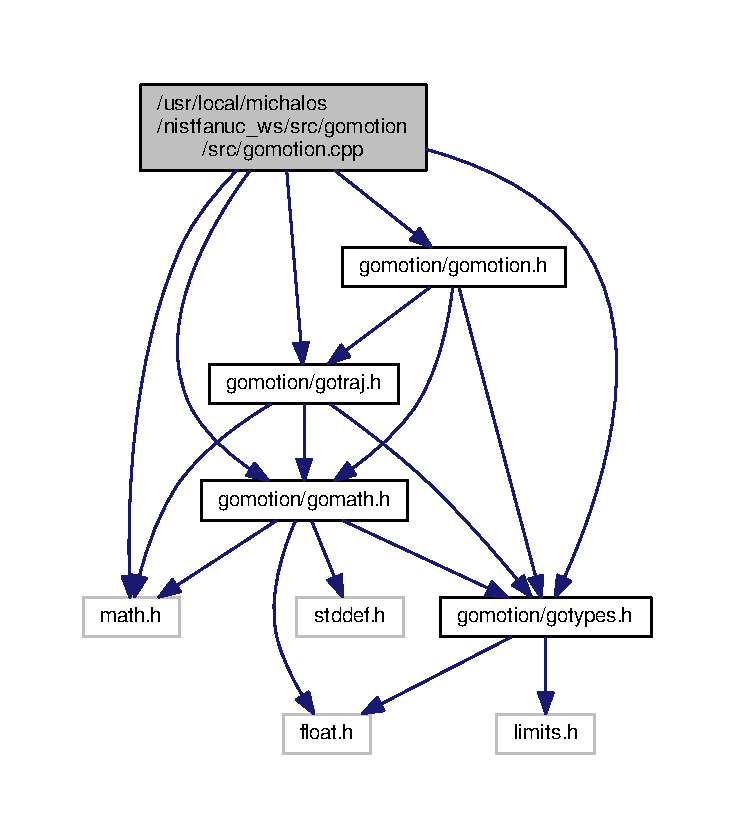
\includegraphics[width=350pt]{d7/d2e/gomotion_8cpp__incl}
\end{center}
\end{figure}
\subsection*{Namespaces}
\begin{DoxyCompactItemize}
\item 
\hyperlink{namespacegomotion}{gomotion}
\end{DoxyCompactItemize}
\subsection*{Macros}
\begin{DoxyCompactItemize}
\item 
\#define \hyperlink{gomotion_8cpp_a012a28e8c92435114d5b5905b009f69e}{maxit}(a, m)~\{if ((a) $>$ (m)) (m) = (a);\}
\end{DoxyCompactItemize}


\subsection{Macro Definition Documentation}
\hypertarget{gomotion_8cpp_a012a28e8c92435114d5b5905b009f69e}{\index{gomotion.\-cpp@{gomotion.\-cpp}!maxit@{maxit}}
\index{maxit@{maxit}!gomotion.cpp@{gomotion.\-cpp}}
\subsubsection[{maxit}]{\setlength{\rightskip}{0pt plus 5cm}\#define maxit(
\begin{DoxyParamCaption}
\item[{}]{a, }
\item[{}]{m}
\end{DoxyParamCaption}
)~\{if ((a) $>$ (m)) (m) = (a);\}}}\label{gomotion_8cpp_a012a28e8c92435114d5b5905b009f69e}

\hypertarget{gomove_8cpp}{\section{/usr/local/michalos/nistfanuc\-\_\-ws/src/gomotion/src/gomove.cpp File Reference}
\label{gomove_8cpp}\index{/usr/local/michalos/nistfanuc\-\_\-ws/src/gomotion/src/gomove.\-cpp@{/usr/local/michalos/nistfanuc\-\_\-ws/src/gomotion/src/gomove.\-cpp}}
}
{\ttfamily \#include \char`\"{}gomotion/gotypes.\-h\char`\"{}}\\*
{\ttfamily \#include \char`\"{}gomotion/gointerp.\-h\char`\"{}}\\*
{\ttfamily \#include \char`\"{}gomotion/gotraj.\-h\char`\"{}}\\*
{\ttfamily \#include \char`\"{}gomotion/gomotion.\-h\char`\"{}}\\*
{\ttfamily \#include \char`\"{}gomotion/gomove.\-h\char`\"{}}\\*
{\ttfamily \#include \char`\"{}gomotion/gomath.\-h\char`\"{}}\\*
Include dependency graph for gomove.\-cpp\-:\nopagebreak
\begin{figure}[H]
\begin{center}
\leavevmode
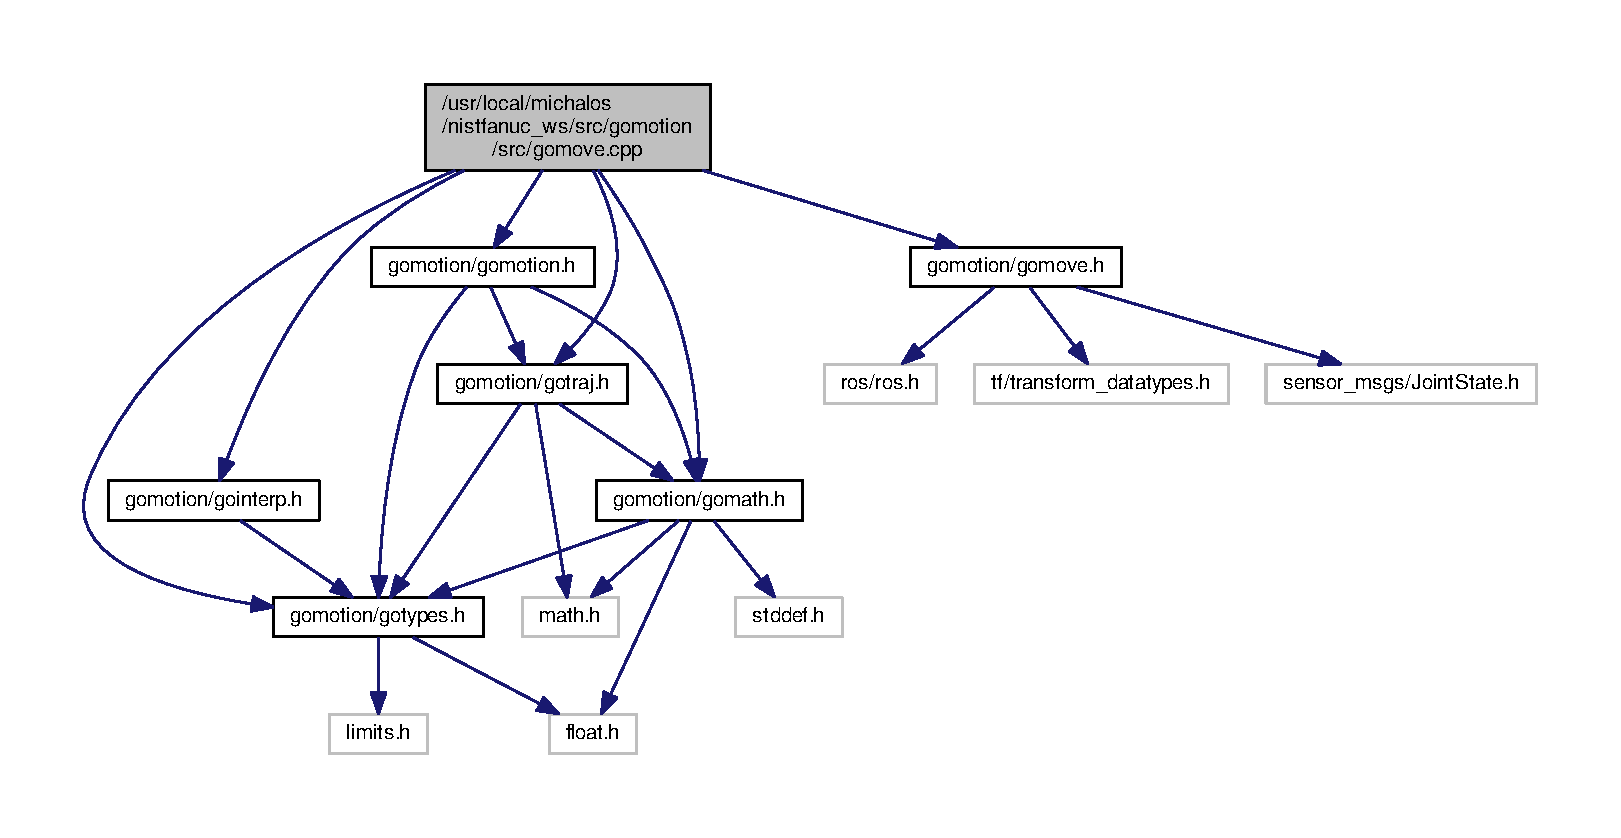
\includegraphics[width=350pt]{d8/dd9/gomove_8cpp__incl}
\end{center}
\end{figure}
\subsection*{Data Structures}
\begin{DoxyCompactItemize}
\item 
struct \hyperlink{structgomotion_1_1go__motion__interface}{gomotion\-::go\-\_\-motion\-\_\-interface}
\end{DoxyCompactItemize}
\subsection*{Namespaces}
\begin{DoxyCompactItemize}
\item 
\hyperlink{namespacegomotion}{gomotion}
\end{DoxyCompactItemize}

\hypertarget{gotraj_8cpp}{\section{/usr/local/michalos/nistfanuc\-\_\-ws/src/gomotion/src/gotraj.cpp File Reference}
\label{gotraj_8cpp}\index{/usr/local/michalos/nistfanuc\-\_\-ws/src/gomotion/src/gotraj.\-cpp@{/usr/local/michalos/nistfanuc\-\_\-ws/src/gomotion/src/gotraj.\-cpp}}
}
{\ttfamily \#include \char`\"{}gomotion/gotypes.\-h\char`\"{}}\\*
{\ttfamily \#include \char`\"{}gomotion/gointerp.\-h\char`\"{}}\\*
{\ttfamily \#include \char`\"{}gomotion/gotraj.\-h\char`\"{}}\\*
{\ttfamily \#include \char`\"{}gomotion/gomotion.\-h\char`\"{}}\\*
Include dependency graph for gotraj.\-cpp\-:\nopagebreak
\begin{figure}[H]
\begin{center}
\leavevmode
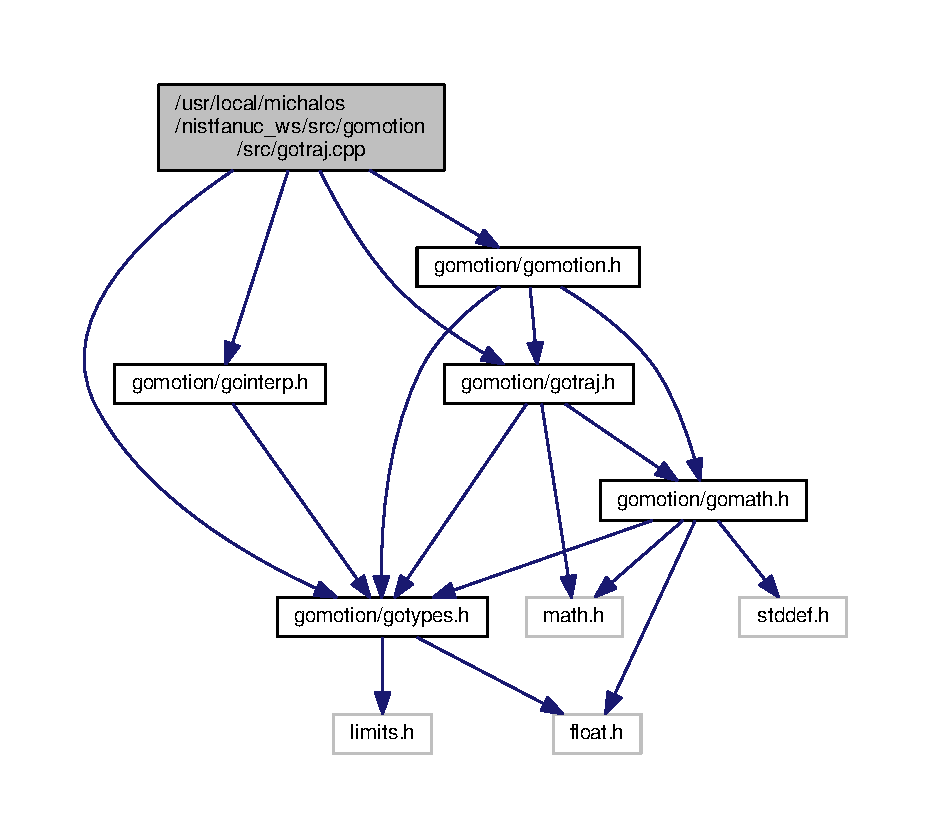
\includegraphics[width=350pt]{d5/de0/gotraj_8cpp__incl}
\end{center}
\end{figure}
\subsection*{Functions}
\begin{DoxyCompactItemize}
\item 
int \hyperlink{gotraj_8cpp_afe14798b0a4a8d9eafedcd8a41ccf3ec}{go\-\_\-init} ()
\item 
int \hyperlink{gotraj_8cpp_ab81e98b9d9bef040e7354f486d860295}{go\-\_\-exit} ()
\end{DoxyCompactItemize}
\subsection*{Variables}
\begin{DoxyCompactItemize}
\item 
int \hyperlink{gotraj_8cpp_a184d14380dbe5f6c91a5038cea6ea6f5}{go\-\_\-result\-\_\-int} = 1
\item 
int \hyperlink{gotraj_8cpp_ac774d0767586d2cfcc72c5a8b2e063a0}{go\-\_\-real\-\_\-double} = 1
\item 
int \hyperlink{gotraj_8cpp_a35b4eb7b07fa8a2c89a4ff5e77a61ca3}{go\-\_\-integer\-\_\-int} = 1
\item 
int \hyperlink{gotraj_8cpp_a5b26be2f7a574d308ae9cbc14c7a8fac}{go\-\_\-flag\-\_\-uchar} = 1
\item 
\hyperlink{gotypes_8h_ae890d9a0ddecc0d3073622cc4312092d}{go\-\_\-flag} \hyperlink{gotraj_8cpp_abb9b839befebbde059804073bd17efd4}{gocode} = 0
\end{DoxyCompactItemize}


\subsection{Function Documentation}
\hypertarget{gotraj_8cpp_ab81e98b9d9bef040e7354f486d860295}{\index{gotraj.\-cpp@{gotraj.\-cpp}!go\-\_\-exit@{go\-\_\-exit}}
\index{go\-\_\-exit@{go\-\_\-exit}!gotraj.cpp@{gotraj.\-cpp}}
\subsubsection[{go\-\_\-exit}]{\setlength{\rightskip}{0pt plus 5cm}int go\-\_\-exit (
\begin{DoxyParamCaption}
{}
\end{DoxyParamCaption}
)}}\label{gotraj_8cpp_ab81e98b9d9bef040e7354f486d860295}
\hypertarget{gotraj_8cpp_afe14798b0a4a8d9eafedcd8a41ccf3ec}{\index{gotraj.\-cpp@{gotraj.\-cpp}!go\-\_\-init@{go\-\_\-init}}
\index{go\-\_\-init@{go\-\_\-init}!gotraj.cpp@{gotraj.\-cpp}}
\subsubsection[{go\-\_\-init}]{\setlength{\rightskip}{0pt plus 5cm}int go\-\_\-init (
\begin{DoxyParamCaption}
{}
\end{DoxyParamCaption}
)}}\label{gotraj_8cpp_afe14798b0a4a8d9eafedcd8a41ccf3ec}


\subsection{Variable Documentation}
\hypertarget{gotraj_8cpp_a5b26be2f7a574d308ae9cbc14c7a8fac}{\index{gotraj.\-cpp@{gotraj.\-cpp}!go\-\_\-flag\-\_\-uchar@{go\-\_\-flag\-\_\-uchar}}
\index{go\-\_\-flag\-\_\-uchar@{go\-\_\-flag\-\_\-uchar}!gotraj.cpp@{gotraj.\-cpp}}
\subsubsection[{go\-\_\-flag\-\_\-uchar}]{\setlength{\rightskip}{0pt plus 5cm}int go\-\_\-flag\-\_\-uchar = 1}}\label{gotraj_8cpp_a5b26be2f7a574d308ae9cbc14c7a8fac}
\hypertarget{gotraj_8cpp_a35b4eb7b07fa8a2c89a4ff5e77a61ca3}{\index{gotraj.\-cpp@{gotraj.\-cpp}!go\-\_\-integer\-\_\-int@{go\-\_\-integer\-\_\-int}}
\index{go\-\_\-integer\-\_\-int@{go\-\_\-integer\-\_\-int}!gotraj.cpp@{gotraj.\-cpp}}
\subsubsection[{go\-\_\-integer\-\_\-int}]{\setlength{\rightskip}{0pt plus 5cm}int go\-\_\-integer\-\_\-int = 1}}\label{gotraj_8cpp_a35b4eb7b07fa8a2c89a4ff5e77a61ca3}
\hypertarget{gotraj_8cpp_ac774d0767586d2cfcc72c5a8b2e063a0}{\index{gotraj.\-cpp@{gotraj.\-cpp}!go\-\_\-real\-\_\-double@{go\-\_\-real\-\_\-double}}
\index{go\-\_\-real\-\_\-double@{go\-\_\-real\-\_\-double}!gotraj.cpp@{gotraj.\-cpp}}
\subsubsection[{go\-\_\-real\-\_\-double}]{\setlength{\rightskip}{0pt plus 5cm}int go\-\_\-real\-\_\-double = 1}}\label{gotraj_8cpp_ac774d0767586d2cfcc72c5a8b2e063a0}
\hypertarget{gotraj_8cpp_a184d14380dbe5f6c91a5038cea6ea6f5}{\index{gotraj.\-cpp@{gotraj.\-cpp}!go\-\_\-result\-\_\-int@{go\-\_\-result\-\_\-int}}
\index{go\-\_\-result\-\_\-int@{go\-\_\-result\-\_\-int}!gotraj.cpp@{gotraj.\-cpp}}
\subsubsection[{go\-\_\-result\-\_\-int}]{\setlength{\rightskip}{0pt plus 5cm}int go\-\_\-result\-\_\-int = 1}}\label{gotraj_8cpp_a184d14380dbe5f6c91a5038cea6ea6f5}
\hypertarget{gotraj_8cpp_abb9b839befebbde059804073bd17efd4}{\index{gotraj.\-cpp@{gotraj.\-cpp}!gocode@{gocode}}
\index{gocode@{gocode}!gotraj.cpp@{gotraj.\-cpp}}
\subsubsection[{gocode}]{\setlength{\rightskip}{0pt plus 5cm}{\bf go\-\_\-flag} gocode = 0}}\label{gotraj_8cpp_abb9b839befebbde059804073bd17efd4}
An ad-\/hoc flag set by various functions that can be used to indicate various code paths taken. 
\hypertarget{gotypes_8c}{\section{/usr/local/michalos/nistfanuc\-\_\-ws/src/gomotion/src/gotypes.c File Reference}
\label{gotypes_8c}\index{/usr/local/michalos/nistfanuc\-\_\-ws/src/gomotion/src/gotypes.\-c@{/usr/local/michalos/nistfanuc\-\_\-ws/src/gomotion/src/gotypes.\-c}}
}
{\ttfamily \#include \char`\"{}gotypes.\-h\char`\"{}}\\*
Include dependency graph for gotypes.\-c\-:\nopagebreak
\begin{figure}[H]
\begin{center}
\leavevmode
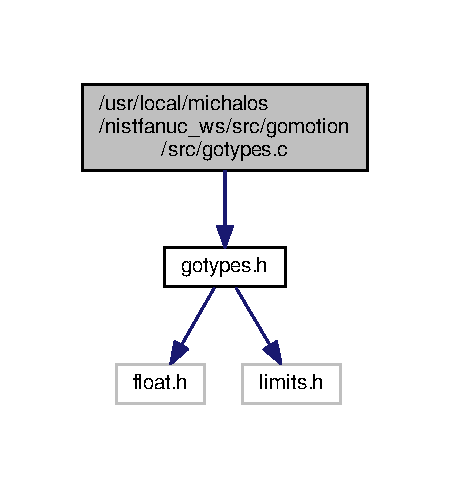
\includegraphics[width=216pt]{da/d14/gotypes_8c__incl}
\end{center}
\end{figure}
\subsection*{Variables}
\begin{DoxyCompactItemize}
\item 
int \hyperlink{gotypes_8c_a184d14380dbe5f6c91a5038cea6ea6f5}{go\-\_\-result\-\_\-int} = 1
\item 
int \hyperlink{gotypes_8c_ac774d0767586d2cfcc72c5a8b2e063a0}{go\-\_\-real\-\_\-double} = 1
\item 
int \hyperlink{gotypes_8c_a35b4eb7b07fa8a2c89a4ff5e77a61ca3}{go\-\_\-integer\-\_\-int} = 1
\item 
int \hyperlink{gotypes_8c_a5b26be2f7a574d308ae9cbc14c7a8fac}{go\-\_\-flag\-\_\-uchar} = 1
\item 
\hyperlink{gotypes_8h_ae890d9a0ddecc0d3073622cc4312092d}{go\-\_\-flag} \hyperlink{gotypes_8c_abb9b839befebbde059804073bd17efd4}{gocode} = 0
\end{DoxyCompactItemize}


\subsection{Variable Documentation}
\hypertarget{gotypes_8c_a5b26be2f7a574d308ae9cbc14c7a8fac}{\index{gotypes.\-c@{gotypes.\-c}!go\-\_\-flag\-\_\-uchar@{go\-\_\-flag\-\_\-uchar}}
\index{go\-\_\-flag\-\_\-uchar@{go\-\_\-flag\-\_\-uchar}!gotypes.c@{gotypes.\-c}}
\subsubsection[{go\-\_\-flag\-\_\-uchar}]{\setlength{\rightskip}{0pt plus 5cm}int go\-\_\-flag\-\_\-uchar = 1}}\label{gotypes_8c_a5b26be2f7a574d308ae9cbc14c7a8fac}
\hypertarget{gotypes_8c_a35b4eb7b07fa8a2c89a4ff5e77a61ca3}{\index{gotypes.\-c@{gotypes.\-c}!go\-\_\-integer\-\_\-int@{go\-\_\-integer\-\_\-int}}
\index{go\-\_\-integer\-\_\-int@{go\-\_\-integer\-\_\-int}!gotypes.c@{gotypes.\-c}}
\subsubsection[{go\-\_\-integer\-\_\-int}]{\setlength{\rightskip}{0pt plus 5cm}int go\-\_\-integer\-\_\-int = 1}}\label{gotypes_8c_a35b4eb7b07fa8a2c89a4ff5e77a61ca3}
\hypertarget{gotypes_8c_ac774d0767586d2cfcc72c5a8b2e063a0}{\index{gotypes.\-c@{gotypes.\-c}!go\-\_\-real\-\_\-double@{go\-\_\-real\-\_\-double}}
\index{go\-\_\-real\-\_\-double@{go\-\_\-real\-\_\-double}!gotypes.c@{gotypes.\-c}}
\subsubsection[{go\-\_\-real\-\_\-double}]{\setlength{\rightskip}{0pt plus 5cm}int go\-\_\-real\-\_\-double = 1}}\label{gotypes_8c_ac774d0767586d2cfcc72c5a8b2e063a0}
\hypertarget{gotypes_8c_a184d14380dbe5f6c91a5038cea6ea6f5}{\index{gotypes.\-c@{gotypes.\-c}!go\-\_\-result\-\_\-int@{go\-\_\-result\-\_\-int}}
\index{go\-\_\-result\-\_\-int@{go\-\_\-result\-\_\-int}!gotypes.c@{gotypes.\-c}}
\subsubsection[{go\-\_\-result\-\_\-int}]{\setlength{\rightskip}{0pt plus 5cm}int go\-\_\-result\-\_\-int = 1}}\label{gotypes_8c_a184d14380dbe5f6c91a5038cea6ea6f5}
\hypertarget{gotypes_8c_abb9b839befebbde059804073bd17efd4}{\index{gotypes.\-c@{gotypes.\-c}!gocode@{gocode}}
\index{gocode@{gocode}!gotypes.c@{gotypes.\-c}}
\subsubsection[{gocode}]{\setlength{\rightskip}{0pt plus 5cm}{\bf go\-\_\-flag} gocode = 0}}\label{gotypes_8c_abb9b839befebbde059804073bd17efd4}
An ad-\/hoc flag set by various functions that can be used to indicate various code paths taken. 
%--- End generated contents ---

% Index
\newpage
\phantomsection
\addcontentsline{toc}{chapter}{Index}
\printindex

\end{document}
